\documentclass[a4paper]{book}


        \def\vismCommit{0b05ee1}

        \def\vismCommitTimestampQuery{in\%20version\%200b05ee1\%20dated\%202024-12-15}

    

\usepackage{multicol}
\usepackage{xcolor}
\usepackage{graphicx}

\def\vismCommitHref{\href{https://github.com/eudoxos/vism/commit/\vismCommit}{\vismCommit}}

% for LaTex, disable plastex parts
\newif\ifplastex\plastexfalse



\ifplastex
	\let\RaggedRight\relax
	\def\marginnote#1{#1}
	%% vism-specific macros for PlasTeX
	\def\vismHypertarget#1{%
		\hypertarget{#1}{}\marginnote{\hyperlink{#1}{\textsuperscript{¶}}}
	}
	\def\vismAssertFootnoteCounter#1{\relax}
	% using \paragraph will insert newline after each heading, so just use \textbf instead.
	\def\vismParagraph#1#2{\hypertarget{#1}{\hyperlink{#1}{\textbf{§#2.}}} }% \vismHypertarget{#1} }
	% used for paragraph alignment in TOC, not useful for PlasTeX
	\def\vismAlignedParas#1{#1: }
	\newenvironment{vismHanging}{}{}
	\def\vismBibIntertitle#1{\bibitem[\textbf{\LARGE #1}]{\textbf{\LARGE #1}}}
\else
	\usepackage[paperwidth=18.2cm,paperheight=23.2cm,a4paper,margin=2.5cm]{geometry}
	% use the same-looking font like BPS2011
	% (they used URWPalladioPali, this is modernized, with unicode glyphs for all pali)
	\usepackage{fontspec}
	\setmainfont{Tex Gyre Pagella}
	% \RaggedRight used in two-column index
	\usepackage{ragged2e}
	% showing anchors and BPS pages in the margin
	\usepackage{marginnote}
	% no page numbers on empty pages
	\usepackage{emptypage}
	%
	\usepackage[protrusion=true,expansion,tracking=true]{microtype}
	%
	\makeatletter
		% https://tex.stackexchange.com/a/31559
		% just hanging pagraphs via parindent/leftskip won't be effective for paragraph after hading (has no \parindent)
		% thus we also need to disable removing indent after heading
		\newenvironment{vismHanging}{
			\bgroup
			\let\orig@afterheading\@afterheading
			\def\@afterheading{\@afterindenttrue\orig@afterheading}
			\parindent=-1em\leftskip=1em\par
		}{\par\egroup}
	\makeatother
	%
	\usepackage{setspace}
	% less warnings
		\hbadness10000
		\vbadness10000
		\hfuzz=10cm
		\vfuzz=10cm
		\parskip=.4\baselineskip
	%% vism-specific macros for LaTeX
	% fix hyperlink in PDF being one line too low, https://tex.stackexchange.com/a/412381
	\makeatletter
	   \newcommand{\vismHypertarget}[1]{
			\Hy@raisedlink{\hypertarget{#1}{}}%
			\marginnote{\footnotesize\textcolor{purple}{#1}}
		}
	\makeatother
	% check that footnote numbers are sequential
	\def\vismAssertFootnoteCounter#1{\ifnum\value{footnote}=#1\else\PackageError{Visuddhimagga}{Footnotes out of sync with original (should be \arabic{footnote}\space, is #1.}\fi}
	% check that paragraph numbers are sequential (disabled by default, as § are not numbered; set \setcounter{secnumdepth}{4} below to enable)
	\def\vismAssertParagraphCounter#1{\ifnum\value{paragraph}=#1\else\PackageError{Visuddhimagga}{Paragraph out of sync with original in \Roman{chapter} (should be §\arabic{paragraph}, is §#1.}\fi}
	% 
	\usepackage{titletoc}
	\usepackage[pagestyles,extramarks]{titlesec}
	\usepackage{ifthen}
	%
	% page header showing paragraphs on the current page
	%
	% straight from titleps (=[pagestyles]{titlesec}) manual
	\newcommand\vismMark{}
	\newshortmark\vismMark
	\def\vismParagraph#1#2{%
		\preshortmark\vismMark%
		\paragraph[§#2.]%
		%{\href{\paraIssueUrl{#1}}{§#2.}}%
		{\hyperlink{#1}{§#2.}}%
		\renewcommand\vismMark{#2}\shortmark\vismMark%
		\vismHypertarget{#1}%
		%\marginnote{\footnotesize\textcolor{purple}{#1}}%
		% \vismAssertParagraphCounter{#2}
	}
	\def\vismAlignedParas#1{\hbox to 5em{#1:\hfill}}
	%% reset paragraphs for each chapter, not subsubsection
	\counterwithout{paragraph}{subsubsection}
	\counterwithin{paragraph}{chapter}
	%
	\def\vismParaPage{
		% use \csname ... \endcsname so that plasTeX does not fail parsing the expression
		\csname ifthenelse\endcsname{%
			\equal{\topshortmark\vismMark}{\botshortmark\vismMark}%
		}{%
			\topshortmark\vismMark%
		}{
			\topshortmark\vismMark–\botshortmark\vismMark%
		}%
	}
	\def\thepageIssue{\href{https://github.com/eudoxos/vism/issues/new?title=issue\%20at\%20page\%20\thepage\&body=(\vismCommitTimestampQuery)}{\thepage}}
	% smaller vertical space above paragraph
	\titlespacing*{\paragraph}{0pt}{\medskipamount}{*2}
	\newpagestyle{vismBody}{
		\setheadrule{.55pt}
		%\headrule
		\sethead[\thechapter.\vismParaPage][\thechapter. \textsc{\chaptertitle}][]{}{\emph{\sectiontitle}}{\thechapter.\vismParaPage}
		\setfoot[\thepageIssue][][\vismCommitHref]{\vismCommitHref}{}{\thepageIssue}
	}
	\newpagestyle{vismNoBody}{
		\setheadrule{.55pt}
		\headrule{}
		\sethead[][\chaptertitle][]{}{\sectiontitle}{}
		\setfoot[\thepageIssue][][\vismCommitHref]{\vismCommitHref}{}{\thepageIssue}
	}
	\renewpagestyle{plain}{
		\sethead[][][]{}{}{}
		\setfoot[\thepageIssue][][\vismCommitHref]{\vismCommitHref}{}{\thepageIssue}
	}
	\pagestyle{vismNoBody}
	% example from titlesec manual, pg 23
	\titleformat{\chapter}[display]{\bfseries\scshape\LARGE}{\filleft\MakeUppercase{\chaptertitlename} \Huge\thechapter}{4ex}{\titlerule\vspace{2ex}\filright}[{%
		\vspace{2ex}%
		\titlerule%
		\vspace*{4pc}%
		\mdseries\normalsize\rmfamily\upshape%
		\startcontents\printcontents{l}{1}[3]{}%
	}]

	% a bit more space for chapter roman number
	\dottedcontents{chapter}[3em]{\bfseries\scshape}{3em}{1pc}
	% tables
	\usepackage{tabularray}
	\NewTblrTheme{vismLong}{
		\SetTblrStyle{firsthead}{font=\bfseries\scshape}
		\SetTblrStyle{middlehead}{font=\bfseries\scshape}
		\SetTblrStyle{lasthead}{font=\bfseries\scshape}
		\SetTblrStyle{label}{}
		\SetTblrStyle{entry}{}
		\SetTblrStyle{caption}{}
		\SetTblrStyle{conthead}{}
		\SetTblrStyle{capcont}{}
		\SetTblrStyle{contfoot-text}{…}
		\SetTblrStyle{conthead-text}{…}
		\SetTblrStyle{rowhead}{1}
	}

	\NewTblrTheme{vismNaked}{
		\DefTblrTemplate{foot}{empty}{}
		\SetTblrTemplate{foot}{empty}
		\DefTblrTemplate{head}{empty}{}
		\SetTblrTemplate{head}{empty}
		\SetTblrOuter{presep=0pt,postsep=0pt}
	}

	% this is only defined in newer versions of tabularray.sty, as the one in the repo here
	% (not yet in TeXLive)
	\RenewDocumentCommand\TblrAlignLeft{}{\RaggedRight}
	% no section for bibliography: https://tex.stackexchange.com/a/132647
	\usepackage{etoolbox}
	\patchcmd{\thebibliography}{\chapter*{\bibname}}{}{}{}

	% fix characters not present in the TeX Gyre Pagella font
	\usepackage{newunicodechar}
	\newunicodechar{ṁ}{\.m}
	\newunicodechar{ḣ}{\.h}
	\newunicodechar{ḳ}{\d{k}}
	\newunicodechar{ṡ}{\.s}
	\newunicodechar{ẏ}{\.y}
\fi

\def\frontmatter{
	\cleardoublepage
	\renewcommand{\thechapter}{\Alph{chapter}}
	\renewcommand{\thesection}{\Alph{chapter}.\arabic{section}}
	\renewcommand{\chaptername}{Front} 
	\ifplastex
		% Part 0 in roman will show as Part, giving Part Front
		%\setcounter{part}{-1}
		\vismUnnumberedPart{Front}{Front}
	\else
		\cleardoublepage
		\setcounter{page}{2}
		\pagenumbering{roman}
		% show in TOC, PDF bookmarks, but don't create titlepage for the part
		\addcontentsline{toc}{part}{Front} 
		%\pdfbookmark[-1]{Front}{front}
	\fi
}
\def\mainmatter{
	\cleardoublepage
	\setcounter{chapter}{0}
	\renewcommand{\thechapter}{\arabic{chapter}}
	\renewcommand{\thesection}{\arabic{section}}
	\renewcommand{\chaptername}{Chapter} 
	\ifplastex\else
		\pagestyle{vismBody}
		\pagenumbering{arabic}
	\fi
}

\def\backmatter{
	\cleardoublepage
	\setcounter{chapter}{0}
	\vismUnnumberedPart{Appendices}{Appendices}
	\renewcommand{\thechapter}{\Alph{chapter}}
	\renewcommand{\thesection}{\Alph{chapter}.\arabic{section}}
	\renewcommand{\chaptername}{Appendix}
	%\appendix\part{Appendices}
	\ifplastex\else
		\pagestyle{vismNoBody}
	\fi
}




% styling of enumerations (roman, alpha, ...); shortlabels for plastex compatibility (label=... does not work for plastex yet)
\usepackage[shortlabels]{enumitem}

\usepackage[hypertexnames=false,bookmarksnumbered=true]{hyperref}
\ifplastex\else\usepackage{bookmark}\fi


% after loading hyperref
\ifplastex\else
	\pdfstringdefDisableCommands{\def\vismAlignedParas#1{#1: }}
\fi

% number chapter with roman numbers
\renewcommand{\thechapter}{\arabic{chapter}}
% show parts as "Part II" in the TOC, but avoid "Part Part II" in the title itself
\renewcommand{\thepart}{Part \Roman{part}}
\renewcommand{\partname}{} 

\def\vismUnnumberedPart#1#2{\part*{#2}\addcontentsline{toc}{part}{#1}}

% deep ToC: subsubsection (4 would mean §§ in the ToC)
% only show subsections in the global ToC
% (but show subsubsections in chapter-level ToCs — in \titleformat{\chapter} above)
\setcounter{tocdepth}{2}
\setcounter{secnumdepth}{3}

\bibliographystyle{abstract}


\ifplastex\else
	\usepackage{newunicodechar}
	\usepackage[weather]{ifsym}
	\newunicodechar{⚡}{\Lightning}
\fi

\def\vismAssertFootnoteCounter#1{\relax}
\begin{document}
	\title{Mastering the Core Teachings of the Buddha}
	\date{work-in-progress \\ ver. \vismCommitHref, compiled \today \\ see \url{https://eudoxos.github.io/vism}  \\ for both \emph{Visuddhimagga} and \emph{Vimuttimagga} in various formats}
	\ifplastex
		\author{by the Arahant \\ Daniel M. Ingram}
	\else
		\author{by the Arahant \\ Daniel M. Ingram}
	\fi
	\maketitle

	\frontmatter
		\renewcommand{\thechapter}{\arabic{chapter}}

		\bgroup
			\ifplastex\else\renewcommand{\baselinestretch}{0.2}\normalsize\fi
			\tableofcontents
		\egroup
		

        \chapter[Credits]{Credits}

            First published in 2018 by

            Aeon Books Ltd

            12 New College Parade

            Finchley Road

            London NW3 5EP

            Copyright © 2018 by Daniel M. Ingram

            The right of Daniel M. Ingram to be identified as the author of this work has been asserted in accordance with §§ 77 and 78 of the Copyright Design and Patents Act 1988.

            All rights reserved. No part of this publication may be reproduced, stored in a retrieval system, or transmitted, in any form or by any means, electronic, mechanical, photocopying, recording, or otherwise, without the prior written permission of the publisher.

            British Library Cataloguing in Publication Data

            A C.I.P. for this book is available from the British Library

            ISBN-13: 978-1-91159-710-0

            Typeset by Medlar Publishing Solutions Pvt Ltd, India

            \href{http://www.aeonbooks.co.uk}{www.aeonbooks.co.uk}

            Printed in Great Britain

            Thanks to my sister \href{http://www.largentcreative.com}{Nancy Largent} for web design and WordPress assistance with www.mctb.org.
        \chapter[Preface to the Second Edition]{Preface to the Second Edition}

            I started writing the small pamphlets and locally printed books that would one day become \emph{Mastering the Core Teachings of the Buddha }(\emph{MCTB1 }hereafter) somewhere in early 1997, which seems quite a long time ago at this point. A lot has changed since then about my own practice, the world of meditation, my understanding of the world of meditation and mental development, and the world in general. The rise of the internet has facilitated unprecedented cross-pollination and collaboration, allowing obscure and isolated practitioners around the world to suddenly come together and share their experiences and ideas about practice. The effect on the dharma has already been profound. I doubt we have seen anything but the tiny beginning of what is possible.

            I would like to thank the numerous people who gave me feedback on the first edition, as I have tried to incorporate every useful piece of advice they offered. In that vein, should you somehow provide feedback on this edition, either good, bad, or otherwise, the more practical and constructive the comments are, the more likely they will have some positive effect on this book.

            The first print edition that was widely available came out in 2008, yet much of it was written during the period of 1997 to 2001, with one major update to the chapter on Models of the Stages of Enlightenment around 2006 to 2007. However, since then many important events have occurred and lots of useful reader and user feedback has been provided that have made me feel that my recently released work was already in need of revision, and so this second edition has come to be.

            Numerous sections have been considerably expanded, particularly the section on concentration, and many things have been rearranged. I have also added an autobiographical section at the end that hopefully will help explain the backstory of some of what you will find in this book. People kept asking for those sorts of details, as well as getting parts of my history very wrong in the absence of that information. Hopefully these points will help clarify things of somepractical value. On the other hand, some people pleaded with me to remove even the small autobiographical details that were in \emph{MCTB1}. I have clearly gone in the other direction, with the basic underlying principle being that I think we should talk (and write) openly about these topics, and not doing so in the previous book clearly had a hypocritical element to it and failed to convey some points that I think are useful for practice and life.

            I have also added more map geekery, as that technical information doesn’t appear in many other places that I am aware of, so I just basically let it rip. Again, these were the details that I wanted when I was coming up in dharma, so I pass these on assuming someone else out there will appreciate them as I did. If it is too much for you, then ignore it, as the basic practices work regardless of whether you are a map-freak like I am.

            I would like to thank members of the Dharma Overground and its sister communities (both living and defunct), without which much in my life and practice simply would not be nearly as good, and for them I am very grateful, as they have enhanced my understanding of the wide world of what is possible and useful in countless ways.

            I hope you will find something in this second edition that helps your practice and enhances your life.
        \chapter[Dedication]{Dedication}

            This book is dedicated to the memory of the late Bill Hamilton.

            His relentless dedication to the cultivation and promotion of wisdom, despite all the consequences, made him a truly great teacher.
        \chapter[Foreword and Warning]{Foreword and Warning\vismHypertarget{foreword-and-warning}}
            \label{foreword-and-warning}


            When I was about fourteen or fifteen years old, I accidentally ran into some of the classic early meditation experiences described in the ancient texts, and my reluctant spiritual quest began. I did not realize what had happened, nor did I realize I had crossed something like a point of no-return, something I would later call the “Arising and Passing Away” (A\&P). I had a very strange dream with bright lights, my entire body and world seemed to explode like fireworks, and afterwards I had to find something, but I had no idea what that was.

            Since then, I have met a large number of people who have also crossed the A\&P early in their lives in various circumstances, many totally unrelated to meditative training. It turns out this is not particularly special or unusual, and I now actually think of it as part of standard human perceptual development. At the time, however, I thought very little about it, having no formal words for it, context to place it in, or understanding of what it was. It got filed into a mental folder for memories of “other weird stuff I don’t know what to do with”, a file that wouldn’t make any sense for about ten more years. I philosophized frantically for years until I finally began to realize no amount of thinking was going to solve my deeper spiritual issues and complete the cycle of practice that had already started.

            I had a friend named Kenneth Folk who played bass in the Motown and soul band that employed me as a sound tech and roadie. We met during my freshman year in college and ended up being housemates in my junior year in a skanky little band house in Chapel Hill, North Carolina. He was in a similar place, caught like me in something we would later call the “Dark Night” and other names. He had crossed the A\&P before moving from California to North Carolina, and it had changed his life in numerous ways. He also realized logic and cognitive restructuring were not going to help us in the end.

            We spent a lot of time playing Frisbee late at night and philosophizing, and finally began looking carefully at what other philosophers had done when they came to the same point, and noted that some of our favorites had turned to mystical practices. We reasoned some sort of non-dual wisdom arising from direct experience was the only way to go, but acquiring that sort of wisdom seemed a daunting, if not impossible, task.

            Kenneth was a bit further along in his spiritual crisis and finally had no choice but to give serious meditation a try. He quit the music business, moved back to the little agricultural desert town of Winchester (near Hemet), California, and lived in a rundown old mobile home his parents owned, driving pizza to save money so he could deepen his spiritual quest. He also was lucky enough to run into a guy named Bill Hamilton. On Bill’s somewhat radical advice, Kenneth did a three-month intensive insight meditation retreat, and then eventually took off to Asia for a year of intensive practice under the guidance of meditation masters in the Burmese Theravada Buddhist tradition. When he came back, the benefits of his practice appeared obvious to me, and a few years later I began to try to follow a similar path.

            In 1994, I began going on intensive meditation retreats and doing a lot of daily practice. I also had some very odd and interesting experiences, and began to look around for more guidance on how to proceed and keep things in perspective. Good teachers were few and far away, their time limited and often expensive to obtain, and their answers to my questions were frequently guarded and cryptic. Even my old music friend was keeping most of what he knew to himself, and issues around disclosure of meditation theory and personal practice details nearly cost us our friendship.

            Frustrated, I turned to books, reading extensively, poring over texts both modern and ancient looking for conceptual frameworks that might help me navigate skillfully in territory that was completely outside my previous experience. Despite having access to an increasing number of great and detailed dharma books, I found they left out lots of details that turned out to be very important. I learned the hard way that using conceptual frameworks that were too idealistic or that were not fully explained could be as bad as using none at all. Further, I found that much of the theory about progress contained ideals and myths that simply did not hold up to reality testing, as much as I wanted them to. The complexities of exactly how this conflict between ideal and reality has morphed over the years are worthy of commentary, and I will discuss this later, after I have set up some important terms and concepts.

            I also came to the profound realization that those darn Buddhists have worked a ton of good stuff out. They have come up with very simple techniques that lead directly to remarkable results if you follow instructions and titrate to the best dose for you. The essential premise that if you want to know more about something you should pay careful attention to it has a simple, elegant brilliance. I wanted to know something essential about my experience and so I paid a lot of attention to it and learned about it. It made sense then and still does. While some people don’t like this sort of cookbook approach to meditation, I am so grateful for the recipes that words fail to express my profound gratitude for the successes they have afforded me. Empiricism has always appealed to me, and Buddhist meditation at its best allows you to see for yourself.

            Thus, as promised, the simple and ancient practices of the Buddha and his followers revealed more and more of what I sought. I found my experiences filling in the gaps in the texts and teachings, debunking the myths that pervade the standard Buddhist dogma, and revealing the secrets meditation teachers routinely keep to themselves. Finally, I came to a place where I felt comfortable writing the book that I had been looking for, the book you now hold in your hands.

            This book is for those who really want to master the core teachings of the Buddha and who are willing to put in the time and effort required. It is also for those who are tired of having to decipher the code often found in modern and ancient dharma books, as it is designed to be honest, explicit, straightforward, and rigorously technical. Like many of the commentaries on texts in the Pali canon, it is organized along the lines of the three basic trainings that the Buddha taught: morality, concentration, and wisdom.

            Throughout this book, I have tried to be as utilitarian and pragmatic as possible. The emphasis is always on how to “get it” at a level that makes some difference. All sections also assume to some degree that you have a practice of some sort, hang out in some form of spiritual scene, and know a bit of the standard dharma lingo. All sections also assume that you are willing to do the work.

            I have tried to include enough information to make this book capable of standing on its own as a manual of meditation and for walking the spiritual path. However, I have also tried to focus on those areas that I consider to be my core competencies and those areas of the spiritual path that I do not feel have been adequately covered in works that have come before this one. This book shines in areas of technique, the maps of meditation, and the fine points of high-level practice. However, the spiritual life is vast beyond measure and cannot possibly be adequately covered in a single book, so I haven’t even remotely tried to make this the complete encyclopedia of meditation or spiritual practices. Thus, I will often refer you to other excellent sources for more details on those topics that I feel have already been covered quite well (and probably better than I could) by other authors. I strongly suggest checking out at least some if not all of those other sources.

            Like my own practice, this book is heavily influenced by the teachings of the late, great Mahasi Sayadaw, a Burmese meditation master and scholar in the Theravada Buddhist tradition, and by those in his lineage and outside it. There are numerous references to other excellent traditions as well, some Buddhist and some not. It is my sincere wish that all diligent students of meditation find something in this book that is of practical value to them, and it is that practical concern for functionality that I hold of greatest value.

            Speaking of pragmatism, there are significant downsides to having the title of this book include the name “Buddha”, as it will likely alienate lots of people who could benefit from the techniques and technical information about the cool, useful, and profound things they can learn to wire their brain to do and perceive. This dismissal based on Uncle Sid’s name might arise in groups as diverse as hyper-rational scientific materialist, or fervent Southern Baptist, or whatever. Also, it is likely that something in my presentation style, which has a bite at times, may cause even some Buddhists to react negatively to valuable Buddhist meditative and conceptual technology. This broader problem of brand and tribal loyalty is rife among nearly all humans. If I say something that offends you based on your rigid allegiances to your particular Buddhist, paradigmatic, or religious brand, and you then dismiss these empowering teachings and fail to employ them to your benefit, the primary loss will be yours, though the effects will likely impact those around you also. This effect is likely to become stronger the farther you proceed into this book. My apologies in advance if I tactlessly play into your knee-jerk tendencies.

            That basic problem of sorting out the gold nuggets of the pragmatic, universal, applicable, technical, helpful, useful, and true from the dogma, proprietary branding, obscure and alienatingterminology, religious craziness, ancient taboos, archaic paradigms, primitive and inaccurate biological assumptions, needlessly rigid frameworks, and other unfortunate aspects of old (and new) traditions is a perpetual problem. This work must be done with care and intelligence, realizing that most of the time we will not get it quite right, as whatever background we come into this task with will limit us to some degree, and this applies to me as much as anyone. So, for those who can go into the old texts, traditions, techniques, communities, cultures, lexicons, and conceptual frameworks with an eye to gleaning why they got so excited about whatever it was that they were doing that they thought was so good (and very likely may be in ways), there is a rich journey of discovery that awaits you.

            One side of me very much wants to write something that is purely secular, utterly devoid of any explicit reference to any ancient frameworks, totally scrubbed of anything religious, and free of any term that is in any way alien to the predominant linguistic sensibilities in the area of the world where I reside. Were this book free from those terms, I naively imagine that it could serve as a general textbook in schools and for scientific study without raising any red flags related to its religious and spiritual references.

            The other side of me rebels equally against this, knowing that for thousands of years the vast majority of the most deeply developed, sophisticated, effective, time-tested, and refined mind-training traditions and insights came straight out of the nunneries, monasteries, jungle huts, mountain caves, and the like from individuals practicing in frameworks of explicitly religious and spiritual traditions, the majority of whom are unlikely to have written things down in the languages you are comfortable with unless you have truly world-class linguistic abilities. There are times when there is no substitute for being able to delve into that vast, complicated, rich treasure trove of artifacts in the old traditions to find what you are looking for. Until that massive amount of theory and practice technology has been translated both linguistically and culturally, which is unlikely to happen anytime soon, we will likely exist in a strange hybrid between ancient and modern, foreign and indigenous, familiar and alien. Luckily, if you are willing to adopt the attitude of the pragmatist over that of the cultural defense warrior (either of your modern culture or of the ancient ones), then you and those in your mind-training social circles can benefit from what you discover.

            On a different note, I have included some of my own experiences in various places and labeled them as such. This is done to try to add some sense of the reality of what is possible, both in terms of successes and failures. They should add a human dimension to the theory. However, if you find that these stories get in the way, or if they seem to have too much of the quality of “let me tell you about my personal spiritual quest,” please do us both a favor and skip over them without a second thought. In this second edition, I have added a more extensive autobiographical section for those who really do want more of the story, but I realize that is not everyone’s cup of tea, so the main body of the theory and practice will leave much of that out and just give you the summary advice that I derived from going through it and learning about the experiences of other fellow adventurers in this amazing territory.

            I have also written this book in what is clearly my own voice. Those who have read this work and who know me tell me that they can almost hear me saying it. I have also left in a lot of my neurotic stuff and made it as obvious as I can. I will assert that anyone who writes puts their neurotic stuff in there even if they try to hide it, so at least you should be able to see it clearlyrather than it being hidden and covert. If you want a book that is just the straight dogma and theory without this sort of voice, there are lots to choose from and I will mention a number along the way.

            I have also included a modicum of social commentary, some of which has a definite bite to it. Some of you may find it not only unhelpful, but even quite distasteful and off-putting. Some of you may quickly dismiss it as harsh or wrong speech. I am torn between the feeling that there really are some important points in those sections, yet understanding that not everyone will be able to make good use of information and opinions presented in such strong terms. Thus, I ask you to please skip over those chapters and get to the friendlier or more technical sections beyond them if you don’t find them helpful. To facilitate doing so, I have included a lightning bolt in the titles of those chapters that contain potentially inflammatory material so that they may be treated appropriately.

            While I feel that the points made in those chapters are important, valid, and useful, they are not absolutely necessary for understanding the chapters that follow them. The world is brimming with very nice and friendly dharma books. There are hundreds available on the shelves of any mega-bookstore. However, I believe that there is room for a book that sometimes conveys its message in a different voice, though I respectfully give you the option to choose how much of that voice you want to hear. It is the unrestrained voice of one from a generation whose radicals wore spikes and combat boots rather than beads and sandals; listened to the Sex Pistols rather than the Moody Blues, wouldn’t know a Beat poet or early ’60s dharma bum from a hole in the ground, and thought the hippies were pretty friggin’ naive, not that we don’t owe them a whole lot. It is also the unrestrained voice of one whose practice has been dedicated to complete and unexcelled mastery of the traditional and hardcore stages of the path rather than some sort of vapid New Age fluff or pop psychological head-trip. If that ain’t you, consider reading something else.

            As a highly regarded senior meditation teacher and scholar (who will remain anonymous) said to me after skimming through an earlier draft of this book, “Most Buddhists are just aging boomers who want to do something to feel better about themselves as they get older and are not really interested in this sort of thing.” I wish them great success in getting those valid needs met. I must reluctantly advise such individuals to avoid reading this book or at least the chapters marked with a lightning bolt. This is simultaneously an admission of the limitations of this work, an invitation to adopt a more empowering view of what is possible on the spiritual path, and a warning.

            I have also been accused of being uncompassionate because I have refused to speak and write in the soft “dharma voice” that is often expected and perhaps seemingly required of people who care deeply about the dharma. I assure you I do deeply care that people eliminate what suffering they can by whatever skillful means necessary and available. I have a real enthusiasm for sharing these truly remarkable concepts and techniques with whoever is interested, hence the free online versions of the book and the free support of a forum for fellow travelers on these strange paths to share the dharma and explore it together.

            I have had other motivations for writing this book. A few people have attempted to have me be their meditation teacher. I have done what I can to encourage them to practice well, go on retreats and explore, but as soon as I get the sense that they are not into really doing the workor are trying to idolize or deify me in even small ways, I go out of my way to return them to themselves, point out distortions caused by transference, and refer them to resources elsewhere. I greatly prefer the company of fellow adventurers who wish to explore the mysteries of this life together than any other sort of relationships, particularly those that potentially disempower one or more of the parties involved.

            Dharma friends may be at different stages in the practice and one friend may teach another something useful, but this has a very different feel from people who are formally ascribed “teacher” and “student”. Thus, writing this book allows me to hand them the better part of what I know and to say, “If you are really into it, there is more than enough here and in the included references to allow you to plunge as deeply as you care to.” If not, I have wasted little of my time and can avoid being put on some strange and dangerous pedestal or pillory, at least to my face.

            That said, I do have the explicit goal of facilitating others to become living masters of this material so that they may go forth and help to encourage more people to do so. The more people can teach from a place of deeply established personal experience, the more people will be able to learn the dharma well, and the saner and happier the world will be. Also, it can just be such great fun to hang out with people who have a real depth of practice and understanding.

            This brings me to the question of the issue of what some would call hierarchy. The simple fact is that there are those who have attained to various degrees of mastery of various aspects of the skills of clear comprehension and the amazing ways we can modify our minds, and there are those who have not. There are those with strong concentration abilities, and those without. There are those who have their morality trip together, and those that do not. There are those who are masters of some techniques and practices, and those that have more work to do.

            While there is a strangely pervasive movement in the West to try to imagine everyone is equal in the world of spirituality (or any other realm for that matter), it is obviously completely delusional and wrong-headed. When I went looking for teachers and friends to practice with and help me along, rather than get mad that some people claimed to know more than I did, and they definitely did, I was excited by the opportunity, however rare, to study with people who knew what they were doing. This just makes sense. Read this as another warning: if you get good enough at these practices, people will often have bad reactions to you if you go around talking about it, and the number who will instead find your achievements a source of inspiration and empowerment, an opportunity to learn something for themselves, as they rightly should, will likely be few.

            On that same front, it is a very strange thing to have such a completely different language, set of experiences, and perspectives from most of the people around me. I can often feel like an alien wearing a trench coat of normalcy, and I dream of a world where conversations about the sorts of events and insights that have come to dominate my everyday experience are much more common and normal. Just like anyone who is truly a fan of some endeavor, in this case one that is fundamental to all the others as it enhances consciousness and attention, it is hard for me to imagine that everyone wouldn’t be totally into this stuff, but for some strange reason most people clearly aren’t.

            Reading between the lines, you should take this admission as yet another warning. If you go way into this stuff, you will discover this same loneliness. Luckily, the online world allowscommunities of those who wish to take this deep to gather and support each other. That said, meatspace is still generally far behind these specialized communities at this point, and so the warning remains valid.

            This should be seen as another warning: this book and the path presented in it are not for those who at this time find that they are unstable spiritual seekers. Meditation at the levels I am about to describe requires a baseline mental and material stability; and with respect to the latter, not necessarily wealth or even a 401(k), but ethically acquired requisites such as food and a safe, conducive shelter. You must have your psychological trip very together to be able to handle and integrate the intense techniques, side effects, and results I am about to discuss. In this book, I will explain in detail what is meant by “have your psychological trip very together”, with the key requisite skills being an ability to identify difficult mind states when they arise and handle them with kindness and aplomb. Luckily these are learnable skill sets.

            There are plenty of gentle techniques and schools of practice available for people for whom it would be more skillful and constructive to apply those techniques. There are also many skillful healing modalities available today to help those who need to heal psychological trauma or clear up barriers to more intense practice. If you need those, you are highly encouraged to do that crucial work first. Many of the techniques and doses recommended in this book are for those who already have a solid platform of mental health and are willing to accept the risks inherent in intensive training.

            Stated much more explicitly: people who do strong and intensive practice can hurt themselves and freak out. Just as serious athletes can hurt their bodies when they take a misstep or push themselves beyond their limits, just so serious mental athletes can strain their minds, brains, and nervous systems, and strained brains can sometimes function in very strange ways. To rewrite the operating system rapidly while it is running doesn’t always go so well in the short term or occasionally in the long term. Thus, while I will include nearly endless exhortations to find the depths of power and clarity that you are capable of, I will also add numerous warnings about how to keep from frying yourself.

            By “frying yourself”, I mean explicitly severe mood instability and psychotic episodes, as well as other odd biological and energetic disturbances, with some practitioners occasionally ending up in inpatient psychiatric facilities for various periods of time. Exactly how much of this is nature (their own “inherent wiring” and potential for mental pathology), how much of it is nurture (practicing hardcore meditation techniques in high doses such as those presented here), and how much is related to other unidentified factors is a question that is still being worked out, just so that you are not in any way uninformed about the still-developing state of modern science as it applies to the art of intensive meditation.

            Some who have read this book apparently have only noticed the former message, that being to find the depths of power and resolution you are capable of (a message put in to counterbalance a culture full of people who are underutilizing or not recognizing their inherent potential), and they missed the parts that discuss how and when to back off, a message found in numerous places in this book, much to their chicken-fried detriment. Hopefully putting this here right up front will again help people to hear both messages and find the balance between the two that works, as I am a firm believer in people being informed not only of the benefits but also of the risks so that they can make informed decisions and practice accordingly. You wouldn’t want todo power lifting without proper training, spotting, and technique, nor run marathons without lots of careful training, stretching, hydration, great nutrition, and the like: same with hardcore meditation practice. You also would be naive to imagine that you can push your body to its limits without risk: same with your brain and hardcore meditation practice.

            I hope that you will find my take on the dharma refreshing, empowering, clear, practical, honest, fair-minded, and open. I have done my best to make it so.

            I would like to thank the very many people whose influence, friendship, support, and kindness went into making this work what it is, though they are way too numerous to list here. This is an interdependent universe, and so to write that this work is simply by me is not in accord with reality. The ideas presented here contain a bit of my synthesis, organization, and phenomenology, a ton of ideas that came to me from people who came before me, and much from contemporaneous practitioners. I feel compelled to mention the specific support of Carol Ingram, Sonja Boorman, David Ingram, Christina Jones, Christopher Titmuss, Sharda Rogell, Bill Hamilton, Kenneth Folk, Robert Burns, Tarin Greco, Vince Horn, and my other friends at the Dharma Overground and its sister sites, all of whom were very instrumental in making what is good in this book and my own practice possible.

            I give a great power-surge of gratitude to my anonymous main editor for this second edition, whose long hours of hard work, kindness, wisdom, heartfulness, patience, and deeply humble love of the dharma both in theory and practice helped to raise this book to a level that it otherwise would not have attained. I would also like to extend deep gratitude to an anonymous patron who helped support this book and shield it from complexity.

            I would also like to thank Duncan Barford, Jeremy Lehrer, Shannon Stein, Elizabeth Pugh, Ann Craig, Peter Stuckings, John Hawley, Roger Windsor, Daniel Rizzuto, Michael Wade for all their editing help and everyone else who informed me of various typos, issues, inconsistencies, errors, and ways this book could be more helpful. Thanks to Oliver Rathbone and Cecily Blench at Aeon for publishing the book and being patient, and thanks to Alan Chapman for suggesting they publish it. However, the responsibility for any flaws this work may contain must fall squarely on me. I can’t be sure that all these fine people would even want their names associated with this work, but I reserve the right to express my deep gratitude nonetheless. Thanks also to Ian Blakely, a.k.a. SEAMO, my stepson, for the cover art.

            A few notes on style. The English language has no great way to use pronouns that refer to a single person without getting gender-specific. Various solutions exist, such as constantly using “he/she” (which can be very distracting), alternating between “she” and “he”, and recasting sentences in the plural, where the pronoun “they” may be used. For better or for worse, I am often going to use the pronoun “they” to mean “he/she”, thus using what is ordinarily a plural pronoun with verbs in the singular. I am not particularly thrilled with this solution, but I don’t think it is much worse than the others. Should a reader disagree, I hope that he/she will find a way to forgive me, or at least that she will understand the problem, making room in his heart for one more author struggling with this linguistic limitation.

            I must also admit that I am somewhat erratic in my use of capital letters, and you may just have to Live with It. I have left in only a few diacritical marks above a few Pali and Sanskrit words, removing most of the rest, as I felt that they are slightly off-putting for many who are not very familiar with them already and thus don’t need them. If you want to look up a specificword and its diacriticals, this information is all widely available on the internet and in libraries. I have also gone slightly rogue in my positioning of commas and periods in relation to quotation marks, mixing a bit of US and UK styles, as I prefer some aspects of both, so my apologies to anyone this disconcerts.

            May this work be for the benefit of all beings. May your practice be for the benefit of all beings. May you aspire to be of benefit to all beings. May you realize what you are truly looking for, pursue it relentlessly despite all obstacles, and find it.
    \mainmatter

    
    \part[The Fundamentals]{The Fundamentals}
        \chapter[Introduction to Part I]{Introduction to Part I}

            If you have not yet read the \hyperlink{foreword-and-warning}{Foreword and Warning}{}, please do so now. The Buddhist path has often been called a “spiritual path”, and this use of religious language can be very inspiring for some people. The Buddhist path can also be thought of in terms of a scientific experiment, a set of exercises that the Buddha and his followers have claimed lead to very specific, reproducible, verifiable effects, which are deemed not just worthwhile but liberative. Using this sort of practical, more scientifically oriented language can also be very inspiring for some people. However, as science doesn’t often provide explicit emphases on the meaning and relevance of its findings to living humans with hearts and minds, language and concepts that can bridge that gap are often useful.

            To inspire a broader audience, I will use both spiritual and practical language when discussing some of the elements concerning the Buddhist path. My preference, however, is generally for the practical language. You could throw out many of the religious trappings of the Buddhist path and still have a set of basic practices that lead to the expected effects. You could also keep all the religious trappings, do the basic practices, and produce the same results, assuming of course that you had the extra time and resources necessary to do both. That said, sorting out which elements are disposable and which are vital for getting the experiment to work is not always straightforward. Some reformative movements can easily go too far when their proponents attempt to remove all elements that don’t fit with their current cultural preferences, aesthetics, and biases. So, it will be for you, me, and our fellow practitioners and adventurers to help sort this out by our own practice.

            In this same pragmatic vein, there has arisen a global movement, inspired by numerous things and promoted by many people, now often referred to as the “Pragmatic Dharma” movement—which I hope one day will be called something more welcoming of those allergic to words such as \emph{dharma}. This movement can be characterized as embracing a worldview that includes the following ideas:
            \begin{itemize}
                \item We can improve the way our minds function and the way they perceive and process reality, in numerous skillful ways.
                \item What works is key. Specifically: it doesn’t matter at all where you draw useful things from if they are effective, meaning that they provide the specific benefits sought.
                \item Innovating by extracting key useful elements from various traditions, and combining things to come up with something that works for you is encouraged, as is pursuing traditional goals in traditional ways, as long as the approach works.
            \end{itemize}

            This book follows this general approach while refraining from being dismissive of elements of great value from the old traditions.

            Part One contains some traditional lists that were taught by the Buddha and relate directly to spiritual training. They make important and practical points in very concise ways. These teachings were presented succinctly on purpose so that people could remember them and use them. It is their very simplicity that makes them so practical and down-to-earth.

            However, I am going to take these very condensed teachings and go on and on about them. It turns out that the Buddha sometimes made things so simple that we, 2,500+ years later, are left wondering what he was talking about and how to apply his teachings to our lives. Still, it is amazing that his teachings are still so relevant to our lives today. These teachings are designed to help people get in touch with their reality in some way that makes a difference. They can also help people avoid some of the common pitfalls on the spiritual path and in life in general, some of which I will talk about later.

            The Buddha’s teachings are also designed to help people develop along some of the nearly infinite \emph{axes of development}. By axes of development, I mean all the ways we can improve our mind, body, and world. Since this is an endless undertaking, in this book we will focus on a relatively few very specific ones. As the book goes along, I will introduce various things we can practice, experience, gain insight into, develop, and modify that make a positive difference.

            Chapter one, “The Three Trainings”, introduces morality, concentration, and wisdom (see also \emph{The Long Discourses of the Buddha}, or the \emph{Digha Nikaya}, sutta 10, usually referred to as DN 10). These three trainings encompass the sum of the Buddhist path. Thus, as is traditional and for good reason, they will be used as the conceptual framework for this book. The three trainings involve skills that we consciously and explicitly try to master. Each training has its own specific set of premises, goals, practices, and standards of mastery for those practices. These are different from each other, and problems can arise if we conflate the premises of one training when pursuing the others. Each training also has its common pitfalls, limitations, and shadow sides, which are rarely made clear, and failure to do so has caused much confusion.

            Thus, I will do my best to make them clear, particularly in Part Two (“Light and Shadows”). The specific standards for success and mastery can sometimes seem a bit technical, particularly the maps of the high concentration states and the stages of insight, so I will wait until Parts Three through Six to present these to keep Part One focused on the basic framework and practices that make the whole thing possible in the first place.

            While I think that each part of this book contributes to the whole, there are reasons you may want to skip to certain sections first and fill in the rest later. For instance, if you are having powerful visions or kundalini experiences, you might want to read the first few chapters of Part Four and then go back and read the rest. If you are simply interested in the maps of the stages of insight, go straight to the chapter called “The Progress of Insight”. If you just want to get right to some core insight practices, read the chapters on “The Three Characteristics” and “The Seven Factors of Awakening”. Should you be in a mood for some social commentary, the beginning of Part Two is for you. If you just want to hear my take on awakening, then “Models of the Stages of Awakening” might be a good place to start. That said, skipping sections is likely to lead to misunderstandings, as plenty of sections that are not close to each other are yet designed to counter excesses that could arise from some other section being read on its own.

            I struggled for a long time over whether to present at the beginning or at the end of the book the maps that detail what these practices lead to. I have included them at the end, but you might be the sort who wants to see them first, and if so firstly you should read the chapter called “The Three Characteristics” and then skip to Part Three.
        \chapter[Morality, The First and Last Training]{Morality, The First and Last Training}

            The original Pali word for this training is \emph{sila}, which I am translating as “morality”. People translate it in various ways. Regardless of the word we choose, it is likely to resonate for people both positively and negatively. If the word “morality” bothers you due to the associations it suggests, look at the assumptions, agendas, and practices of this training and come up with your own word for it. I don’t think that it is so important what we call it. I do, however, think that we should give careful attention to trying to live it.

            From my perspective, training in morality has as its domain all the physical, verbal, and mental behaviors belonging to every single aspect of life that is not explicitly meditative. When we are trying to live a good life in the conventional sense, we are working on training in morality. When we are trying to work on improving our physical, emotional, and mental health, we are training in morality. When we philosophize, we are training in morality. When we exercise, we are training in morality. When we are taking care of others or ourselves, we are training in morality. When we try to guard the environment by not misusing or wasting resources, reform corrupt governments, or make this world a better place for everyone, we are training in morality. When we commit to a non-harming and benevolent livelihood, build a healthy marriage, raise healthy children, or shave our heads and move to a remote place to dedicate ourselves to intensive spiritual practice, we are training in morality. Whatever we do in the ordinary world that we think will be of some benefit to others and ourselves is an aspect of working on this first training.

            I should add a qualifier here, relating to what a life well-lived might mean. For some, that is a life of riches, decadence, and hedonism. That is not what I am talking about. It is not that wealth is inherently bad, though there are strong moral arguments to be made for a vastly more equitable distribution of wealth. It is not that all decadence is inherently bad, and I would hate to make someone feel terrible for having a second dessert occasionally, but clearly there is a great degree of spending on luxury that is contributing to the destruction of the planet and behavior that simply leads to more misery for all concerned in the name of “fun”. It is not that we shouldn’t enjoy our lives, as an enjoyable life is a much easier one to accept, but clearly plenty of the pathways people go down seeking enjoyment do predictably lead to more suffering than they produce pleasure or fulfillment. So, with those qualifiers in mind, ponder what a life well-lived would mean and aspire to that.

            The third training, called wisdom, as understood within the Theravada framework, has limits, in that you can only take it so far, and it can be fully mastered. Interestingly, this cannot be said of the first two trainings of morality and concentration. There is no limit to the degree of skill that can be brought to how we conduct ourselves in the world. There are so many ways we can develop, and no obvious ways to define what one hundred percent mastery of even one of these might be. Thus, morality is also the last training in the sense of being the training we need to cultivate throughout our lives. We may be able to attain to extraordinary states of consciousness and understand many aspects of the actual nature of sensate reality, but what people see and what is causal are the ways that these abilities and understandings translate into how we live in the world. Some folks who read \emph{MCTB1}, for reasons I am unsure of, came away with the mistaken impression that I somehow consider morality as unimportant. Let me now be completely clear on this: morality cultivated throughout our entire lives is critical for everyone, and particularly for those who want to train in concentration and wisdom!

            There are basic premises that are extremely helpful when undertaking training in morality. It is very helpful to accept, for example, that a basic moral code, that is, a universal and non-harming ethic, is helpful for getting along in this world, and thus that there is practical, real-world benefit to be derived from training in morality.

            It is also helpful to accept in an easygoing and non-dogmatic way, that the more good we do in the world, the more good there will appear in that world both for us and for others, and thus the more good things will happen to us and all others. It is also worth assuming the corollary of this, which is that the more we do harmful actions in the world, the more harm we experience and therefore the more that miserable circumstances arise.

            These premises are not unique to Buddhism, nor are they in any way extraordinary, and that brings me to an important point about the spiritual traditions in general: most religions have points that are generically useful that they have attempted to appropriate as exclusively theirs, such that extremist followers of that faith may come to believe that their tradition’s teaching on morality is the only teaching on morality. The corollary of this fallacy is that people not of their own religion are considered unlikely or incapable of being truly moral, when, in fact, societies and traditions throughout the ages and around the world have advocated for a universal, non-harming ethic.

            It is worth realizing that defining “negative” and “positive” action is often very much a question of perspective. In the face of this, some will retreat into the semi-dysfunctional and often self-serving position of moral relativism, in which we decide that morality is totally subjective or that morality is arbitrary and thus futile or unnecessary to bother with. Paradigms that are less intellectual and more grounded in common sense can help us to avoid falling into the paralyzing and extremely dangerous trap of imagining that it is futile to train in morality, however seemingly relative and arbitrary. It is better to try to do our best and fail than not to try at all.

            Thus, the Buddha taught that what we think, say, and do has consequences for our subsequent moment-to-moment experience. When undertaking training in morality, we are proceeding from the premise that we can, if we choose, control what we think, say, and do, thus creating consequences that are pleasant and beneficial, both in terms of our experience and that of others. Rather than accepting our current level of intellectual, emotional, and psychological development as being beyond our power to change, we consciously and explicitly adopt the empowering view that we can work with these aspects of our lives and change them for the better. We assume that we do have the capacity to change our world and our attitudes towards our world. We take responsibility for our actions and their consequences.

            Further, as a part of our empowerment, we assume that the more we bring our resources and abilities to this training, the likelier we are to succeed. We have a body, we have reason, we have our intuition, we have our heart, and we can learn and remember. We have a community of others who have wisdom to share, we have books and other media that contain advice for living a good life, and we have our friends and family. We can draw on all these and more to try to live a good life, a life in which our thoughts, words, and deeds reflect as closely as possible the standards we have consciously adopted and defined for ourselves. The more consciously engaged we are with our task, the more we are likely to be successful.

            Crucial to the control of what happens in our lives is our intention. Thus, training in morality places much emphasis on intention, with the basic assumption being that the more our intentions are kind and compassionate, the more we are likely to be able to manifest kind and compassionate thoughts, words, and deeds.

            Further, it is helpful to understand that training in morality requires us to pay attention to what is happening in our lives. When we are not paying attention to what we are thinking, saying, and doing, we will not easily be able to craft these in a way that fits with the assumptions of this training. If we are not paying attention to the consequences of our thoughts, words, and deeds, both in the short and the long terms, we are unlikely to be able to gain enough experience to be able to successfully carry out our training in morality.

            It is also helpful to understand that training in morality will help us when we get to formal meditation practices (the next two trainings in concentration and wisdom), providing a foundation of good mental and physical habits that can support those practices, as well as helping to avoid the mental and physical irritation that can result from a lack of a solid moral foundation. Thus, even if for some crazy reason, we have little interest in being moral because of the benefits it brings, if we are interested in obtaining the results of the other two trainings, we must also engage in training in morality.

            These key points about training in morality naturally lead to the specific agendas we have for what happens when undertaking training in morality. We consciously aspire to have the actions of our body, speech, and mind fit with the premises or prerequisites of this training. In short, we have standards for our mental, emotional, and physical lives and we try our best to live up to those standards. When we are training in morality, we consciously cultivate actions, words, and thoughts that we deem to be non-harming, and if possible, kind and compassionate. By “kind”, I mean that we work to promote the happiness and welfare of others and ourselves. By “compassionate”, I mean that we work to understand and relieve the suffering, problems, or unhappiness of others and ourselves. Thus, our agenda is for our intentions to be kind and compassionate, for our minds to be aware of what we are thinking, saying, and doing, and for our experience to inform us how best to craft our life to reflect our wisely informed good intentions.

            Training in morality tends to be discussed in terms of what we should and shouldn’t do. The standard Buddhist short list of the five actions that practitioners should refrain from doing are referred to as the five precepts: killing, stealing, lying, taking intoxicants that lead to heedlessness, and sexual misconduct, which includes such actions as cheating on a partner or using sexuality in a harmful way (\emph{Sutta Nipata} [SN] 2.14). These are not unique to Buddhism, and seem to be part of the basic set of standards for behavior that societies and cultures throughout the ages have found to be helpful and practical. The standard list of things that we should try to do includes being kind, compassionate, and appreciative of the successes of others.

            Additionally, in the \emph{Karaniya Metta Sutta} (SN 1.8), we find the following advice: “Those who are skilled in good and wish to attain the state of peace should be able, upright, perfectly upright, compliant, gentle, and humble. Contented, easily supported, of simple livelihood, with few duties, controlled in senses, discreet, not impudent, they should not be carried away by the emotions of the majority. They should not commit any slight wrong such that the wise ones might censure them.” The rest of the sutta is also very worthy of reading and practicing.

            Wrestling with the question of how we can meet these standards and yet honor where we are and what is going on around us is the training in morality. We will make all kinds of mistakes that can be very educational when trying to work on this first training; if you mess up, remember to be gentle with yourself!

            There are many great techniques for cultivating a more decent way of being in the world, but there are no magic formulas. You must figure out how to be kind to yourself and all beings in each moment. Since training in morality considers all the ordinary ways in which we try to live a beneficial and useful life, it is so vast a subject that I couldn’t possibly give anything resembling a comprehensive treatment of it here.

            Some have criticized the first edition of this book for not going deeply enough into the specifics of morality. It is a fair criticism, but I think that it has already been done well in so many other places, such that if you wish to explore the basics of training in morality as approached in the context of Buddhist traditions, I suggest that you check out some of the following works and look around for others that inspire you to take care of yourself and the world around you: \emph{For a Future to be Possible}, by Thich Nhat Hanh; \emph{A Heart as Wide as the World} and \emph{Loving­kindness: The Revolutionary Art of Happiness}, both by Sharon Salzberg; \emph{Light on Enlightenment}, by Christopher Titmuss; and \emph{A Path with Heart}, by Jack Kornfield.

            There are excellent resources available online and in books; those of you who want to get deeper into Buddhist ethics might want to explore the morality practices of both the Theravada and the Mahayana trainings. The Mahayana has teaching systems of the Mind Training or Lojong tradition, which offer very refined practices for developing exceptional kindness and consideration. Those with a taste for more controversial aspects of the dharma might look towards John Stevens’ \emph{Lust for Enlightenment: Buddhism and Sex}. I personally also look to the work of Dan Savage for many relative aspects of navigating modern adult lay life.

            Training in morality at its best is grounded in a theoretical or direct appreciation of one more vital recognition, that of interdependence. Interdependence at this level means an appreciation of the fact that we are all in this together and that we all share the wish to be happy and avoid misery. When we take into consideration our own needs and the needs of those around us, we are more likely to be naturally kind and considerate of others and ourselves. Thus, we try to make it a habit to consider the welfare, feelings, and perspectives of those around us. The obvious potential trap here is to simultaneously fail to consider our own needs. Work on balancing both in a way that is sustainable and healthy.

            There are countless other pitfalls we can run into when training in morality, as mastering our behavior of body, speech, and mind is not easy, especially if we were not raised with particularly helpful role models. I will spend a lot of time in Part Two detailing some of the more common side effects and shadow sides of training in morality, but please understand it is a vast subject.

            One pitfall that must be addressed here, however, since it is so common, is guilt. We in the West have grown up in a relatively privileged culture in which we can be extremely hard on ourselves, causing ourselves staggering amounts of pain to little good effect. If we can learn to substitute wise remorse, which simply says, “Well, that didn’t work, and that is unfortunate. I will try my best to figure out why and hopefully do something better next time,” we will be much better able to train successfully in living a good and useful life.

            Some people unfortunately seem to think that the primary message of training in morality is that they should continuously cultivate the feeling that they have taken up a heavy yoke of responsibility and self-oppression. In fact, some people seem to revel in that unfortunate feeling. Those more fortunate will think, “It is so much fun to try to live a good, healthy, and useful life! What a joy it is to find creative ways to do this!” There are few things more helpful on the spiritual path and for life in general than a positive attitude. Thus, the related and all too common pitfall is that people stop having fun, stop having a sense of humor (a definite red flag of something gone awry if you ask me) and stop trying to be successful in worldly terms. There is absolutely no reason for this.

            If you can have fun in healthy ways, have fun! It’s not just for breakfast anymore. Also, success is highly recommended for obvious reasons. Pick a flexible vision of success in the ordinary sense for yourself and go for it! Play to win. This is your life, so make it a great one. There is no reason not to try, as long as you can do so in a kind and compassionate way. The basic spirit is that these trainings are fun, a magnificent adventure in learning and growing, a remarkable opportunity to have many fascinating and transformative experiences, a wonderful experiment in what is possible in this life: these attitudes make a huge difference in all the trainings we will discuss here.

            One more great thing about training in morality is that it is indispensable for the next training: concentration. So, here’s a tip: if you are finding it hard to concentrate because your mind is filled with guilt, judgment, hatred, resentment, envy, or some other harmful or difficult thought pattern, work on the first training. It will be time well spent. Further, if and when you start doing more intensive training, you will very quickly realize that whatever good mental and psychological habits you have will be a great support, and whatever unskillful mental habits you bring will definitely slow you down or even stop you. Do spend your non-retreat time cultivating a healthy mind, a healthy body, and a skillful and mature set of coping mechanisms.

            I was on a retreat in 2003 with a mighty meditation master named Sayadaw U Pandita Jr., so named to differentiate him from the late meditation master Sayadaw U Pandita, who was a senior monk and one of Venerable Mahasi Sayadaw’s direct successors, and author of such classic books as \emph{In This Very Life}, and \emph{On the Path to Freedom} (both of which I recommend). The former gave a long talk on the Pali word \emph{danta}, meaning “tamed” or “restrained”. He explained it as carrying the qualities of being poised, dignified, and stable. “Restrained” means refraining from ill-conceived or harmful (to oneself and others) actions of body, speech, and mind. Practicing with a sense of ourselves as being dignified, mature, capable, balanced, poised, steady, and able to be comfortable in our own skin while doing simple things like sitting and walking: this way of working and seeing yourself is of great benefit all around.

            So, we now have a good, and quite large list of things to work on, and so begins the list of the axes of development. I used to play a game called Dungeons and Dragons back in the day (geek much?), and it was and still is a fantasy role-playing game in which we take on the role of a character who has specific attributes. In the old version of the game that I played, player characters would have various degrees of strength, intelligence, wisdom, dexterity, constitution, and charisma, with standard humans having values for each of those ranging from three to eighteen, with three being the lowest possible level and eighteen being as high as humans could normally achieve. For instance, were I to have a character with the following attributes: strength 13, intelligence 18, wisdom 9, dexterity 17, constitution 11, and charisma 4, I would be very smart, not very wise, quite dexterous, extremely uncharismatic, and average in other factors.

            Just because a character had developed one of these qualities didn’t mean the others were well developed. In D\&D, these qualities were generally fixed entities unless something unusual happened. However, in the game we are playing in the real world, we assume that the various qualities we wish to develop are not fixed qualities that we can’t improve on, but instead can definitely be cultivated and improved upon, perhaps beyond what we ever imagined.

            Thus, were we to draw up a character sheet for our progress in the three trainings in their various complicated aspects and track them over time, we might notice that various abilities improved with time in some generally upward trend as we gave them attention, realizing that the inevitable declines and setbacks that come with time may happen as well. So, let’s say we wanted to create the part of our own character sheet that dealt with some very simplified axes of development of the vast training of morality, we might come up with something that looks like this:

            Kindness toward ourselves

            Kindness toward others, both humans and non-humans

            Ability to set and respect reasonable boundaries

            Written communication ability

            Spoken communication ability

            Ability to skillfully support ourselves

            Ability to skillfully support others

            Generosity

            Patience

            Gratitude

            Persistence

            Honesty

            Integrity

            Dedication to service

            Ability to pace ourselves to work up to our potential without burning out

            Support of physical health (which we might break down further into diet, exercise, sleep, etc.)

            Academic development

            Intellectual understanding of models of healthy human development

            Emotional maturity

            Development of ethics

            Sense of humor

            Intellectual curiosity/enjoyment of learning

            Common sense

            Skillful relationships with people

            Skillful relationships to mind-altering substances

            Skillful relationship to power

            Skillful relationship to sexuality

            Skillful relationship to money and possessions

            Skillful relationship to politics

            Skillful relationship to our spiritual achievements and less developed areas

            Etc.

            This list I have come up with is very arbitrary and woefully incomplete, and is meant to serve as a general example of a concept, not a definitive guide, and I would encourage you to take time to consider what your own list would look like and how you have done over the years, as well as what you aspire to in the future, since explicit goals and frameworks help galvanize and direct energy for progress.

            A point that will be repeated in this book is that success in one of these areas doesn’t guarantee success in the others, and what one person considers success, someone else might not. For example, an aid worker in some war-torn refugee camp and a politics-renouncing solitary hermit might hold different opinions on how best to use their time to help save all beings. This is an essential concept when it comes to all these trainings and axes of development that is often not well understood; just because you may be strong in one developmental skillset doesn’t necessarily translate into being strong in the others. Just because you have developed one to a degree and in a way that suits your ideals doesn’t mean anyone else will hold that view. Too often, models of spirituality assume that just because you have one practice or skill down that you will necessarily have some others, what I call the “package models”. While there are some examples of people who do get packages of benefits that arrive together, there are just as many exceptions to those rules.

            While learning specific things can help us learn related things more easily, such as people who play the violin well might be able to more quickly pick up guitar or cello, plenty of skill sets don’t translate to other areas of our life. This applies not only to you but also to your dharma companions, teachers, etc. The most common example of relevance is that just because someone may speak well, look good, be well-educated, be a dharma scholar, or even have strong meditative abilities, doesn’t mean they will necessarily have such things as good interpersonal and communication skills, or skillful relationships with power, money, or sex. I talk about this more later. In the meantime, it is time to move on to a discussion of the second training, concentration.
        \chapter[Concentration, The Second Training]{Concentration, The Second Training}

            Concentration is the ability to steady the mind on whatever you wish and attain unusual and profound altered states of consciousness. Training in concentration relates to formal meditation practice, though some of these states can arise spontaneously during other activities. The second training is also called training in “samadhi” (meaning depths of meditation), or sometimes “samatha”\emph{ }(Pali) or “shamatha” (Sanskrit) practice. The word “samadhi” is used differently in various traditions, with the Theravada using it as a near equivalent of shamatha, but some traditions, such as some of the Indian Vedantic traditions and some of the Mahayana traditions, use it to describe high states of realization (Vedantic) and extremely high levels of deep concentration (Mahayana), so please be careful when using the word “samadhi” and be aware when reading it that it can mean very different things to different authors. My apologies in advance for people who prefer “samatha” or “shamatha”, as I will use these terms interchangeably.

            Concentration practice involves working at a level that might be considered unusual, particularly when contrasted with the ordinary level of training in morality. Training in morality is something nearly everyone can relate to, at least to some degree. Buddhism frames all the trainings in terms of the reduction of suffering and the liberation of mind, and while reduction of suffering is easy for most people to relate to, liberation of mind in the grand classical sense is not. Training in concentration is only easy to relate to if you have attained to unusual states of consciousness or at least have faith that they can be attained.

            Training in concentration has had thousands of pages dedicated to it, and there are probably thousands of concentration exercises. Some very commonly used objects of meditation are the breath (my personal favorite), our posture, a mantra or koan, a colored disk, an image, a candle flame, various visualized objects from simple to complex, feelings such as compassion, and even the experience of concentration itself. The object you choose should be one on which you would be happy to steady your mind.

            The essential point about meditation is this: \emph{to get anywhere in meditation you need to be able to steady the mind and be present in the present}. That’s all there is to it and it is largely a question of just doing it. There is an important shift that happens in people’s practice when they really make the commitment to develop concentration and follow through with it. Until we do this, not much is likely to happen in our meditation practice!

            If you decide to do a concentration practice, stay on the chosen object like a dog with a bone until you have enough stability and skill such that the mind can rest on it effortlessly. Let me say here that there are various types of concentration, with the relevant distinction being continuous concentration versus moment-to-moment concentration. Both types develop concentration, but they feel different. For this section, I am talking about continuous concentration, which feels steady, smooth, and analog, rather than the concentration required to investigate individual sensations moment by moment that will be addressed when I discuss training in insight.

            The first formal goal when training in continuous concentration is to attain what is called “access concentration”, meaning the ability to remain focused on your chosen object with relative ease to the exclusion of distractions. This is the basic attainment that allows you to access the higher stages of concentration and to begin the path of insight, which is the third training, so make it a priority to attain access concentration in your meditative practice. The first edition of this book said, “You will know it when you have it,” but I have realized that I was very wrong regarding this, and I also underestimated the different standards people have for what they consider access concentration. Regardless, for the sake of discussion, when you can keep your attention on your object of meditation second after second, minute after minute, without letting it go to other objects, but before any interesting, blissful, unusually steady alteration of perception happens, that is what I call access concentration.

            To digress before I continue, those who wish to define “access concentration” some other way, please do, just realize that we may have a problem here, with this being the first instance of what I call “term wars”, which highlight the fact that there really should be multiple qualifiers of a term or even multiple terms for various experiences. However, we have for this whole range of accomplishments only one term from the sanctified past. We end up with various factions struggling to control the meaning of that sanctified single term, in this case “access concentration”, but also, as we will see, nearly all the other map terms as well. What generally happens is that, instead of doing the intelligent thing, which is to recognize that we need more terms, and instead of using those, we mostly just battle it out in sectarian ways like dysfunctional, territorial academics.

            For example, let’s say that some guy whose initials are something like BAW and I want to define “access concentration” very differently. Perhaps we could have “DMI access concentration” and “BAW access concentration” to help distinguish the usages, as neither is likely to want to give up their use of the term “access concentration”, and yet each may be using it to describe states of mind that are significantly different. By using the qualifiers, we can at least realize which set of criteria are being used.

            However, just as I tend to loathe eponymous medicine (e.g. Colles’ fracture, Hansen’s disease, etc.), I don’t like eponymous meditation terms. Hopefully, by enough non-eponymous qualifiers related to things like depths of attainment, degree of stillness, steadiness of focus (and duration, for those who like duration as a criterion), etc., we will have some idea of what we mean rather than warring over single terms that are clearly inadequate to describe the wide range of meditation territory in a way not bound up in individual practitioners and authors. I have this odd notion that Buddhists, who often pride themselves on their terminological sophistication, precision, and mental clarity, will come together from across the traditions and cultures (just like the chemists did back in the day to systematically standardize the nomenclature for molecules, and as mathematicians did for mathematic notation) and do the same for meditative attainments. That, unfortunately, would require us all getting over ourselves and getting on with the work of bringing meditation into the twenty-first century. Don’t hold your breath, as it were. Back to the instructions.

            The essential formal concentration practice instructions are: pick an object (the list on page 13 is a great place to begin), find a place to practice where you are as free from distractions as possible, pick a sustainable posture in which the spine is relatively straight (it doesn’t really matter so much, but for this training it helps if it is somewhat comfortable), focus your attention on the object as completely and consistently as possible for the duration of that practice period, allowing as few lapses in concentration as possible, and learn to stabilize all of your attention on that object. The more you practice and the better your practice, the better you will become at concentrating. Find the balance of effort and steadiness that works for you.

            If your effort is too light, your mind will slide off the object, but if it is too tight you will wind yourself up and be too tense to settle into steady concentration. Be kind to yourself when the mind wanders, returning it with minimal fuss to the object of concentration again and again. Practice again and again until you can attain access concentration. Tune in to anything smooth, flowing, and nice about what you are concentrating on and experiencing. While these two paragraphs may seem trite or sparse, they contain the formal instructions on how to begin training in concentration. More advice on the proper balance of mental factors is given shortly.

            Should you need someone to tell you how long to practice, start with ten minutes a day and work up to an hour or two each day as your life allows. If you can learn to hold your attention completely on your chosen object for even one solid minute, you have some strong concentration skills. That said, you might have ten or more hours a day to devote to practice. Don’t let me hold you back! If you can go on retreat and do this sixteen or more hours a day, even better, as you would be amazed how in just a few days of that sort of high dose many people can get into very interesting meditation territory if they practice well. How long it will take you to develop access concentration depends on multiple factors including practice conditions, your natural and cultivated concentration ability, the strength of your drive to succeed, and how much you practice.

            Sharpening your concentration may help almost everything you do, and can provide mental and emotional stability that can be very useful, translating to many other areas of your life. Concentration can also lead to very pleasant states referred to as “jhanas”. These can be extremely blissful and peaceful. Being able to access these states of mind can be ridiculously enjoyable and profound. These states are valuable in and of themselves and serve the important function in the Buddhist tradition of providing a disposable foundation for insight practice, in that you can build those states up and then tear them down with investigation of the sensations that make them up, which is the third training.

            I will leave off describing the specific concentration attainments until Part Three to keep this section focused on the essential skills necessary for meditation, as once you gain access concentration, getting into those states is relatively easy. Until you gain access concentration, you ain’t got squat. Thus, pick an object, practice well and often, attain access concentration, finish reading this book, and by that point everything should be straightforward.

            The world of concentration is vast and contains within it myriad skills that can be developed to remarkable degrees. As the number of objects that we can get good with and the many ways we can tune our minds are remarkably complex, it is hard to clearly delineate a simple and manageable inclusive list of all the things we can learn in the vast realms of concentration. However, were we to try, we might start with the following:
            \begin{itemize}
                \item The speed with which we can get into skillful altered states of awareness (generally called here “concentration states” or “jhanas”).
                \item The depth to which we can get into each of those states.
                \item The number of objects that we can use to get into each of those states.
                \item The stability of those states in the face of external circumstances.
                \item The various ways we can fine-tune those states (such as paying attention to and developing their various sub-aspects).
            \end{itemize}

            I will talk more about this in Part Three, saving this section for the more fundamental aspects of training in concentration. Now, it must be said that concentration practices, like all practices, have their shadow sides. For instance, pleasant and unusual experiences can become addictive and extremely seductive, causing us to give them more attention and focus than they deserve or than would be beneficial to deeper practice. They can also lead to people becoming way “out-there” and ungrounded, very much the way hallucinogens can. They can cause the “real world” to seem harsh by comparison, causing us to be tempted to reject the world, withdraw, or dissociate into the world of concentration states. They can also bring up lots of our psychological “stuff”. This last limitation could be a benefit if we were in a mood to deal maturely with our stuff. Perhaps the most important limitation of concentration practices is that they do not lead directly to the insights and irreversible realizations that come from training in wisdom, as much as we might like them to. That brings us to the third training …
        \chapter[Wisdom, The Third Training]{Wisdom, The Third Training}

            The third training in the list is wisdom, in this case a very special kind of wisdom that I will often call “ultimate” or “fundamental” wisdom. This may also be rendered as “understanding” or “insight”. The whole trick to this training is to understand some specific aspects of the sensations that make up our present experience. By training in insight, we can improve how we fundamentally perceive reality at a bare sensate level, such that our actual sensate experience becomes progressively clearer. This increased clarity can become hardwired into our brains, such that our baseline degree of sensate clarity increases. This increased clarity can have numerous positive and sometimes surprising implications. Great meditators from all traditions have reported that there is something remarkable and even enlightening about our ordinary experiences if we take the time to investigate them very carefully. Those who undertake training in wisdom have decided to conduct the experiment to see for themselves if this is true or if those long-gone dudes and dudettes were just making it up.

            Let’s begin by taking it as a wholesome given that there is some understanding that is completely beyond any ordinary understanding, even beyond the skillful altered states of consciousness that can be attained if we train well in concentration. The next premise is that there are specific practices that can and will lead to that understanding if we simply do them. The third and perhaps most vital premise is that \emph{we can do these specific practices and be successful}.

            The given—rarely stated explicitly but often implied—is that we must be willing to stay on a sensate level, at the level of the actual sensations that make up experiences, if we wish to gain the promised insights. The corollary of this premise is that we must be willing to set aside periods of practice time during which we abandon ordinary ways of functioning in the world and even the unusual way of working with skillful altered states of consciousness that belongs to the training in concentration. We proceed from the premise that the teachings on wisdom point to universal truths that can be perceived in all types of experience without exception. We accept that if we can simply know our sensate experience clearly enough, we will arrive at fundamental wisdom.

            Most “insight meditators” spend their time doing a lot that relates to the ordinary world and/or to cultivating refined states of consciousness, and they don’t realize that this is not insight practice. I define insight practice extremely narrowly, as opposed to morality, which I define extremely broadly, and concentration, which I define more narrowly but which is still a broader topic. Insight practice is all about putting those broader ways of working aside and instead grounding attention in our six sense doors and their true nature. While there are clear overlaps among the trainings, even on the cushion, I feel that to try to counterbalance our strong habits of working more broadly is of value to most practitioners. If you happen to be one of those rare people who can focus just on your sense doors as they arise and vanish and while setting aside focus on morality and concentration, then this paragraph is not for you.

            There are many wisdom traditions and many styles of insight practice. I will lay out several explicitly and hint at many others in the chapters that follow. When choosing an insight tradition, look for one that is tried and true, meaning that it is either ancient and well-tested, or contemporary but demonstrably consistent in leading to unshakable realizations. I can verify that the specific practices I will present can lead to the promised effects if they are done as recommended. Even better—you should verify them for yourself.

            The primary purpose for doing insight practices is to increase our perceptual abilities so that the truths accessed by skilled meditators become obvious. Thus, rather than caring what we think, say, or do, or caring about what altered state of consciousness we are in, when training in wisdom, we actively work to develop the clarity, resolution, precision, consistency, and inclusiveness of the experience of all of the constantly changing sensations that make up our experience, whatever and however they may be: such are the formal insight practice instructions.

            Insight practice can seem more daunting, complex, or bizarre than other forms of practice. However, it is oddly simple. There are six sense doors. Sensations arise and vanish. Notice this for every sensation. These are cave-man simple instructions, yet somehow people make them much more complex than they need to be. As a preview of things to come, towards the very end of the book you will see me repeat this same message as basically the punch-line to the whole book, since that was what I found the most profound and helpful of all the Buddha’s teachings. So, should you find your practice getting bogged down in fascinated or aversive reactions to the fancy and flashy topics that follow, return here, as this points to where the real treasure is: your own immediate sensate reality.

            Just as with concentration practices, more time and more diligent practice pays off. These simple instructions can easily seem overwhelming, vague, or strangely trivial to many people, so I am going to detail numerous empowering concepts and more structured practices that have helped countless practitioners over centuries to follow these basic instructions. That said, the above-mentioned are the key instructions.

            While the three trainings share similar elements, there are important distinctions that must be made between them.

            The gold standard for training in morality is how consciously harmless, kind, skillful, and compassionate our intentions, words, and actions are and how well we lead a useful and moral life.

            The gold standard for training in concentration is how quickly we can enter into specific, skillful, altered states of consciousness on our own meditative power, how long we can stay in them, and how refined, complete, and stable we can make those states.

            The gold standard for training in wisdom with insight practices is that we can quickly and consistently perceive the true nature of the countless quick sensations that make up our whole reality, regardless of what those sensations are, allowing us to cut to a level of understanding that goes utterly beyond specific conditions but includes them all.

            It is vital that these distinctions be understood. Considered this way, these gold standards do not overlap and may even appear to contradict one another, when in fact they support each other. As these distinctions seem to be extremely difficult to explain clearly, I will make this basic point again and again throughout this book.

            Having gained at least enough morality to be temporarily free of agitating negative mind states and enough concentration to steady the mind, turn your attention to the bare truth of the sensations of this moment. This is called insight meditation, which is designed to produce a form of knowledge or wisdom that can transform and free us from our core perceptual misinterpretations of sensate reality.

            Sounds simple, and while it \emph{is} simple, it’s not easy in practice. There are many types of insight that we may derive from experiencing the world. Usually, we might think of training in wisdom as having to do with conventional issues like how to live our lives. In this sense, we might just try to be wiser. Perhaps we could skillfully reflect on a personal or professional situation that went badly and see if perhaps in the future some wisdom gained from that experience might change the way we live our life. This is an ordinary form of wisdom, and so the insights we derive from such reflections and observations are insights into the ordinary world. Such reflections are clearly skillful, but they can only take us so far. To really get what the Buddha was talking about, we need to go beyond these conventional notions of wisdom and attain to ultimate insights by engaging specifically in insight practices.

            Many people try to make insight practices into an exercise that will produce both insights into the ordinary world and ultimate insights. There are numerous traditions that specifically advocate for this sort of practice that attempts to work on both fronts simultaneously. However, I have concluded that we should not count on ultimate teachings to illuminate or resolve our relative issues or vice versa. Therefore, it is extremely important not only to practice all three trainings, but also not to conflate the relative and ultimate wisdom teachings. Failure to do so causes endless problems and makes progress more difficult. Thus, I will revisit this topic throughout this work, doing my best to clearly differentiate those practices that produce ordinary wisdom from those that fall within the third training and lead to awakened perceptual transformations that are distinct from our relative insights.

            A brief note of caution here: occasionally, when people begin to get into spirituality, they may get a bit fascinated with it and may forget some of the crucial relative wisdom, otherwise known as common sense, that they may have learned from before. Caught up in “ultimate wisdom” and their “spiritual quest”, they can sometimes abandon conventional wisdom or discernment and other aspects of their “former life” to a degree that may not be particularly skillful. They falsely imagine that by training in insight they have mastered or gone beyond the training in or need for morality. We awaken to the actual truth of our life in all its conventional aspects, so make sure that yours is a life you want to wake up to.

            In summary, by seeing deeply into the truth of our own experience, profound and beneficial transformations of consciousness are possible. You guessed it—we’re talking about awakening, nirvana, nibbana, the unconditioned, and all of that. The arising of this understanding is the primary focus of this book. There are many fascinating insights that typically occur even before awakening. Again, there are no magic formulae for producing ultimate insights, except for the three characteristics …
        \chapter[The Three Characteristics]{The Three Characteristics}

            The three characteristics of impermanence, dissatisfactoriness, and no-self are so central to the Buddha’s teachings that it is almost inconceivable how little attention the majority of “insight” meditators give them. I cannot possibly overstate the usefulness of trying again and again to really discern these three qualities of all experience. They are the stuff from which ultimate insight at all stages comes, pure and simple. Every single time I say, “Understand the true nature of things,” what I mean is, “Directly perceive the three characteristics.” To perceive them thoroughly and directly is to be awakened.

            Somehow this exceedingly important message doesn’t typically seem to get through to insight meditators, so they spend much time doing anything but looking precisely, moment to moment, into the three characteristics. They may be thinking about something, lost in the stories and tape loops of the mind, trying to work out their stuff, philosophizing, trying to quiet the mind, or who knows what, and this can go on retreat after retreat, year after year, decade after decade, and of course they wonder why they don’t have any insight yet. This is a tragedy of monumental proportions, but you do not have to be part of it! You can be one of those insight meditators who knows what to do, does it, and finally gets it in the truest sense.

            The big message here is: drop the stories. Find a physical object like the breath, the body, pain, or pleasure, some feeling of resistance you may be experiencing, etc., and train yourself to perceive the three characteristics precisely and consistently. Drop to the level of bare sensations. This is vipassana, insight meditation, the way of the Buddhas. All the “opening to it”, “just being with it”, “letting it go”, and so on are quite important, as we will see later, but insight meditators must—I repeat, must—look into the following:
            \section{Impermanence}

                All experienced phenomena, whether physical or mental, inner or outer, are impermanent. This is one of the most fundamental teachings of the Buddha and the second-to-last sentence he uttered before he died:

                \emph{All phenomena are impermanent! Work out your salvation with diligence!}

                In his last words, he said everything you need to know to do insight practices. Things come and go. Nothing lasts for even a microsecond. Absolute transience is truly the actual nature of experiential reality.

                What do I mean by “experiential reality”? I mean the universe of sensations that you directly experience. There are many gold standards for reality. However, when doing insight practices, the \emph{only} useful gold standard for reality is your own sensate experience. From the conventional perspective, things are usually believed to exist even when you no longer experience them directly, and are thus inferred to exist with only circumstantial evidence to be relatively stable entities. Predictability is confused with continuity of existence. For our day-to-day lives, this assumption is functional and adequate.

                For example, you could close your eyes, put down this book or device, and then pick it up again where you left it without opening your eyes. From a pragmatic point of view, this book was where you left it even when you were not directly experiencing it. However, when doing insight practices, it just happens to be much more useful to assume that things are only there when you experience them and not when you don’t. Thus, the gold standard for reality when doing insight practices is the sensations that make up your reality\emph{ in that instant}. Sensations that are not there at that time are not presumed to exist, and thus only sensations arising in that instant do exist, with “exist” clearly being a problematic term, given how transient sensations are.

                In short, most of what you assume as making up your universe doesn’t exist most of the time, from a purely sensate point of view. This is exactly, precisely, and specifically the point. Knowing this directly leads to freedom.

                For you philosophers in the crowd, this is basically British empiricism taken to its logical extreme and then hardwired through repeated practice. I think the great Scot, David Hume, would have loved the assumptions of insight practices. I am in no mood to debate questions of ontology, but, for the specific task of progressing in insight practice, this empirical extreme simply works. Thus, I view empiricism through a utilitarian lens and recommend you do likewise when doing insight practices: accept that things you do not experience directly do not exist in that moment. When doing basically everything else, accept they probably do. Those sets of assumptions lead to better outcomes, and better outcomes are my primary objective.

                Regarding impermanence, it is wise to reflect on our own mortality, a common reflection in many Buddhist traditions, for it is useful and true. This is a reflection on ordinary reality and thus an aspect of training in morality that is commonly used to develop motivation to train in insight. I gained some dharmic benefits and relative insights from the one hundred and sixty hours we spend in medical school dissecting a corpse down to shreds. However, when practicing insight meditation, it is far better to perceive one sensation arise and pass away. What do I mean by this? I mean that sensations arise out of nothing, do their thing, and vanish utterly. Gone. Entirely gone. Then the next sensation arises, does its thing, and disappears completely. “That‘s the stuff of modern physics,” we might say. “What does that have to do with practice?”

                It has everything to do with practice! We can experience this, because the first set of vibrations we have access to isn’t actually that fast. Vibrations. That’s right, vibrations. That’s what this first characteristic means: that sensate reality vibrates, pulses, appears as discrete particles, is like TV snow, the frames of a movie, a shower of vanishing flower petals, or however you want to say it.

                Some people can get all into complex wave or particle models here, but do yourself a favor and don’t. Just examine your actual experience, especially something nice and physical like the motion and sensations of the breath in the abdomen, the sensations of the tips of the fingers, the lips, the bridge of the nose, beneath the nose and above the lip, or the subtle tingling on the scalp and so on. Instant by instant, try to know when the actual physical sensations are there and when they are not. It turns out they are not there a good bit of the time, and even when they are, they are changing constantly.

                We are typically quite sloppy about distinguishing between physical and mental sensations (memories, mental images, and mental impressions of other physical or mental sensations). These two kinds of sensations alternate, one arising and passing and then the other arising and passing, in a quick but perceptible fashion. Being clear about exactly when the physical sensations are present will begin to clarify their slippery counterparts—flickering mental impressions—that help co-create the illusion of continuity, stability, or solidity.

                Immediately after a physical sensation arises and passes is a discrete pulse of reality that is the mental knowing of that physical sensation, here referred to as “mental consciousness” (as contrasted with the problematic concept of “awareness” in Part Five). By physical sensations I mean the five senses of seeing, hearing, smelling, tasting, and touching, and I guess you could add some proprioceptive, other extended sensate abilities and perhaps a few others, but for traditional purposes, let’s stick to these five. This habit of creating a mental impression following any of the physical sensations is the standard way the mind operates on phenomena that are no longer actually there, even mental sensations such as seemingly auditory thoughts, that is, mental talk (our inner “voice”), intentions, and mental images. It is like an echo, a resonance. The mind forms a general impression of the object, and that is what we can think about, remember, and process. Then there may be a thought or an image that arises and passes, and then, if the mind is stable, another physical pulse.

                Since I just used this dangerous term “mind”, I should quickly mention that it cannot be located. I’m certainly not talking about the brain, which we have never experienced, since the standard for insight practices is what we can directly experience. As an old Zen monk once said to a group of us in his extremely thick Japanese accent, “Some people say there is mind. I say there is no mind, but never mind! Heh, heh, heh!”

                However, I will use this dangerous term “mind” often, or even worse “our mind”, but just remember when you read it that I have no choice but to use conventional language, and that in fact there are only utterly transient mental sensations. Truly, there is no stable, unitary, discrete entity called “mind” that can be located! By doing insight practices, we can fully understand and appreciate this. If you can do this, we’ll get along just fine.

                Each one of these sensations (the physical sensation and the mental impression) arises and vanishes completely before another begins, so it is possible to sort out which is which with relatively stable attention dedicated to consistent precision and to not being lost in stories. This means that the instant you have experienced something, you can know that it isn’t there anymore, and whatever is there is a new sensation that will be gone in an instant.\emph{ }There are typically many other momentary sensations and impressions interspersed with these, but for the sake of practice, this is close enough to what is happening to be a good working model.

                Engage with the preceding paragraphs. They are the basis of great insight practice. Given that you now know that sensations are vibrating, pulsing in and out of reality, and that, for the sake of practice, every sensation is followed directly by a mental impression, you now know exactly what you are looking for. You have a clear standard. If you are not experiencing it, then stabilize the mind further, and develop more clarity about exactly when and where there are physical sensations. Spend time with this, as long as it takes. The whole goal is to experience momentariness directly, that is, things flickering, and what those things are doesn’t matter one bit!

                How freeing! Interpretation is particularly useless in insight meditation, so you don’t have to spend time doing it when you are on the cushion. Throughout this book, I recommend reflecting on spiritual teachings and how to bring them to bear on life when off the cushion. Thoughts, even supposedly good ones, are just too slippery and seductive most of the time, even for advanced meditators, though if you can avoid getting lost in their content they are as valid a stream of sensate objects for insight practices as any other. When doing insight practices, try to limit yourself to no more than a few minutes of skillful reflection per hour of meditation. This should be more than enough. There are simply no substitutes for this sort of momentum in practice. If you can get that reflection down to no minutes at all, so much the better.

                How fast are things vibrating? How many sensations arise and vanish each second? This is exactly what you are trying to experience, but some very general guidelines can provide faith that it can be done and perhaps point the way as well. Begin by assuming we are initially talking about one to ten times per second. This is not actually that fast. Try tapping five to ten times per second on a table or something. It might take two hands, but it’s doable, isn’t it? You could experience that, couldn’t you? That’s the spirit!

                Not good at counting beats per second? Here’s a quick trick. If you count, “one, one-thousand”, at a steady pace, that is about one second per “one, one-thousand”. Notice that it has four syllables. So, you are counting at four syllables per second, or 4 Hertz (Hz), which is the unit of occurrences per second. If you tapped your hand each time you said or thought a syllable, that would be four taps per second. Try it! Count “one, one thousand” and tap with each syllable. So, you now know you can experience at least eight things in a second! You experienced the four syllables and the four taps that went along with them. You probably experienced all sorts of other things also, like sights, sounds, other physical sensations, and a lot more during that one second. Yay! That is insight practice. You are already up to at least eight sensations per second. Yay, you!

                Let’s say you tapped twice per syllable. That would already be up to at least twelve things you perceived in a second, the four syllables and the eight taps. That actually isn’t that hard to do. You are already fast enough to really bust out some insight practices. Great job! Investigate reality that fast and you will learn some seriously cool things. Add in noticing the intentions to tap each of those taps and the mental impressions of all of the sensations you just experienced, and suddenly you are rockin’ it like a boss in the world of insight meditation.

                There are faster and slower vibrations that may show up, some very fast (maybe up to forty times per second or so) and some very slow (that are actually made up of faster vibrations), but let’s just say that one to ten times per second can sometimes be a useful guideline in the beginning. Once you get the hang of it, the faster and slower vibrations are no big deal. Alternately, depending on how you practice, conceiving of this as like a shower of raindrops, an animated pointillist painting, or 3D TV snow might help. Reality is quite rich and complex, and thus the frequencies of the pulses of reality can be somewhat chaotic, but they tend to be more regular than you might expect. Also, there are not any “magic frequencies”. Whatever frequency or pulse or whatever you are experiencing at that moment is the truth of that moment. However, in the beginning you should go for faster vibrations over slower ones and then later try for broader and more inclusive ones over those that are narrower.

                Don’t worry if things look or feel solid sometimes. Just be with the solidity clearly and precisely, but not too tightly, and that pattern of sensations that implies solidity can start to reveal its impermanence. Be aware of each exact moment in which you experience solidity and its beginning and ending. Remember that each experience of solidity is a discrete, impermanent sensation. Also, some people find things like counting frequencies and using numbers totally annoying, so, if you are one of those, just ignore those parts, as direct experience is the key regardless of whether you can count beats well. Still, the general concept that you are looking for something changing moderately fast but still quite manageable is key. “Let it go,” as those kooky Buddhists sometimes say.

                Many people begin practicing and really want to solidify something like the breath so that they can finally pay attention to it. They become frustrated when they have a hard time finding the breath or their body. The reason they can’t find these is not that they are a bad meditator but that they are having direct insight into how things actually are! Unfortunately, overemphasizing the theory and concepts of concentration practice, which aims to perceive the meditation object as more solid and stable, creates much needless frustration for the insight practitioner who doesn’t know better. You should now be able to avoid a lot of that frustration and begin to appreciate why knowing some theory about the difference between insight and concentration practices is helpful.

                It is also worth noting here that the frequency or rate of vibrations may change often, either getting faster or slower, and that it is worth trying to perceive clearly the beginning and ending of each vibration or pulse of reality. These are actually at least two different sensations! It is also useful to check out exactly what happens at the bottom, middle, and top of the breath if you are using the breath as an object, and to examine if the frequency remains stable or changes in each phase of the breath. Finding the exact end of the out-breath is a commonly used exercise of great profundity once mastered. Never assume that what you have understood is a final, fixed answer. Be alert. Explore carefully and precisely with openness and acceptance. This is the door to understanding.

                One last thing about vibrations: exploring vibrations can be a lot like any other sport. We can think of it the same way as we would of surfing or playing tennis, and this playful game-like attitude can help a lot. “We’re out to bust some vibrations!” as Kenneth enthusiastically put it. You don’t know quite what the next return or wave is going to be like, so pay attention, keep the mind on the pulse of the sensations of your world just as you would on the wave or ball, and keep playing!

                I highly recommend this sort of speed in practice not only because that is how fast we must perceive reality to awaken, but also because trying to experience one to ten sensations per second is challenging and engaging. Because it is challenging and engaging, we will be less prone to getting lost in thoughts rather than doing insight practices. Our minds have the power to perceive things extremely quickly, and we actually use this power all the time to do such things as read this book. If you don’t use that massive resolving power, you are likely to quickly get really bored and wander off to something more interesting. You can probably read many words per second. If you can do this, you can certainly do insight practices.

                If you can perceive one sensation per second, try for two. If you can perceive two unique sensations per second, try to perceive four. Keep increasing your perceptual threshold in this way until the illusion of continuity shatters. \emph{In short, when doing insight practices, constantly work to perceive sensations arise and pass as quickly and accurately as you possibly can}. With the spirit of a race car driver who is constantly aware of how fast the car can go and still stay on the track, stay on the cutting edge of your ability to see the impermanence of sensations quickly and accurately.

                I will relate four of the many little exercises that I have found useful for jump-starting and developing insight into impermanence. They will demonstrate how we can be creative in exploring our reality precisely, but please don’t think of them in some dogmatic way. These objects and postures are not that important, but understanding impermanence directly is.

                In one of these exercises, I sit quietly in a quiet place, close my eyes, put my right hand on my right knee, my left hand on my left knee, and concentrate just on my two index fingers. Basic dharma theory tells me that it is not possible to perceive both fingers simultaneously; so, with this knowledge, I try to see in each instant which one of the two fingers’ physical sensations are being perceived at any given moment. Once the mind has sped up a bit and become more stable, I try to perceive the arising and passing of each of these sensations. I may do this for half an hour or an hour, just staying with the sensations in my two fingers and perceiving when each sensation is and is not there.

                This might sound like a lot of work, and it can be until the mind settles into it. It requires the concentration of a fast sport like table tennis. This is such an engaging exercise and requires such precision, making it hard to get lost in thought if I am really applying myself. I have found this to be a very useful practice for developing momentary concentration and debunking the illusion of continuity. You can pick any two aspects of your experience for this exercise, be they physical or mental. I generally use my fingers only because through experimentation I have found that it is easy for me to perceive the sensations that make them up.

                In another, related exercise, I do the same sort of thing, sit quietly in a quiet place with eyes closed, but instead I concentrate on the sensations of the front and back of my head. With the knowledge that the illusion of a separate perceiver is partially supported by one impermanent sensation incorrectly seeming to perceive another impermanent sensation which it follows, such as the sensations in the back of the head incorrectly seeming to perceive the sensations of the front of the head, I try to be really clear about these sensations and when they are and are not there. I try to be clear if the sensations in the head are from the front or the back of the head in each instant, and then try to experience clearly the beginning and ending of each individual sensation. You can also do this with the sides of the head, as well as the sensations that seem to be in the middle of your head.

                This practice also requires a table tennis-like precision. Half an hour to an hour of this can be quite a workout until the mind speeds up and becomes more stable, but this sort of effort pays off. As I mentioned above, when I am engaged with this practice, there is little room to be lost in thought. I have also found this a very useful practice for developing concentration and for debunking the illusions of continuity and of a separate self (more on that later). A few have reported that this exercise makes them nauseated or dizzy, which may come from applying too much effort and not gently allowing these sensations to just reveal themselves easily and naturally. If that happens to you, be gentle and let the sensations of the front and back of the head show themselves to you naturally.

                In another exercise, which is quite common to many meditation traditions, I sit quietly in a quiet place, close my eyes, and bring my attention to the breath. More than just concentrating on it, I know that the sensations that make up the concept “breath” are each impermanent, lasting only an instant. With this knowledge, I try to see how many individual times in each part of the breath I can perceive the sensations that make up the breath. During the in-breath I try to experience it as many times as possible, and try to be precise about exactly when the in-breath begins and ends.

                More than this, I try to perceive exactly and precisely when each sensation of motion or physicality of the breath arises and passes. I then do the same for the out-breath, paying particular attention to the exact end of the out-breath and then the beginning of the new in-breath. I don’t worry about how I am breathing because it is not the quality of the breath that I am concerned with or even what the sensations are, but one aspect of the ultimate nature of these sensations: their impermanence, their arising and passing away.

                I also don’t care much about exactly where I am experiencing the breath, as the breath is experienced in many places from nose to back to pelvis. Some traditions get particularly picky about where you notice the breath, so if you want to give one of those a try, don’t let my bias towards finding it wherever it is hold you back. When I am fully engaged with bending the mind to this exercise of following the many rich and varying sensations of breathing, there is little room to be lost in thought. I have found this to be a very useful practice for developing moment-to-moment concentration and penetrating the illusion of continuity.

                In the last exercise, I take on thoughts directly. I know that the sensations that make up thoughts can reveal the truth of the three characteristics, so I have no fear of them; instead, I regard them as more glorious opportunities for gaining insight. Again, sitting quietly in a quiet place with eyes closed, I turn the mind to the thought-stream. However, rather than paying attention to the content as I usually do, I pay attention to the ultimate nature of the numerous sensations that make up thoughts: impermanence. I may even make the thoughts, which are typically occurring in the general region of my head, more and more intense just to get a good look at them.

                It is essential to try to perceive how you experience thoughts at a sensate level, otherwise you will likely flounder in their content. What do thoughts feel like? Where do they occur? How big are they? What do they look like, smell like, taste like, sound like, feel like? How long do they last? Where are their edges? Only take on this practice if you are willing to try to work at the level of trying to discern what thoughts actually are rather than what they mean, represent, or imply. If we begin to explore carefully, we will realize that thoughts are made of many types of sensations, sounds, sights, physical feelings, even tastes and smells, but they will often, though not always, be associated with one predominant sense door.

                If my thoughts are more auditory, as in inner talk, I begin by trying to perceive each syllable of the current thought and then each syllable’s beginning and ending. If they are visual, as in mental images, I try to perceive every instant in which a mental image presents itself. If they seem physical, such as the memory of a movement or bodily sensation, I try to perceive exactly how long each little sensation of this memory lasts.

                This sort of investigation can be fairly easy to do and yet is quite powerful. Things can also get odd quickly when doing this practice, but I don’t worry about that. Sometimes thoughts can begin to sound like the auditory strobing section of the song “Crimson and Clover”, where it sounds like they are standing at a spinning microphone. Sometimes the images that arise internally can begin to flash and flicker. Sometimes our very sense of attention can begin to strobe. This is the point! The sensations that imply a mind and mental processes are discontinuous and fleeting.

                Again, this practice requires steadiness and determination, as well as precision. There is no time to be lost in the content of the thoughts, as I am trying too hard to be clear about the beginning and ending of each little flicker, squawk, and pulse that makes up a thought. This can be an especially fun practice when difficult thoughts, thoughts that have sticky or emotionally heavy content for me, are distracting from a physical sensation. I can turn on them, break them down into meaningless little blips, little vibrations of suchness, and then they don’t have the power to cause me any trouble. They just scatter like confetti. They are seen as they are: small, quick, and harmless. They have a message to convey, but then they are gone.

                When I am done with this exercise, I return to physical objects and their arising and passing. However, I have found taking on the sensations that make up thoughts to be another very useful exercise for developing momentary concentration and penetrating the illusion of continuity. It doesn’t matter if they are “good thoughts” or “bad thoughts”, as all mental sensations are also dripping with ultimate truth that is just waiting to be discovered, and thus I can proceed in my investigation with confidence regardless of what arises. Whether our illusions are penetrated using physical sensations or mental sensations is completely irrelevant, but from another point of view it is really good to be skilled at doing both, which comes with practice.

                Hopefully these exercises will give you some idea about how we might practice understanding impermanence. Impermanence is a quality whose clear perception leads to wisdom, so just understanding this again and again can be enough to drum it into our thick heads, debunk the illusion of continuity, and once this is drummed into our thick heads we are freer.

                This can be a subtle business, so be patient and persevere. Remember all three trainings of morality, concentration, and wisdom. Following flickering sensations and understanding the other two characteristics of suffering and no-self that they manifest can be a powerful and direct cause for deep insights and awakenings.

                For five years of my practice I was mostly a “one technique freak”, and that technique was noticing how sensations flicker. I would do it as often as I could, that is, whenever I didn’t have to be doing something that required concentration on the specifics of my life. I would be riding an elevator, just trying to see when I could feel each foot, or lying down to sleep and noticing how many times I could experience the sensations of my breath in each second. I also tried to notice this aspect of things for every single sensation that occurred during my formal practice. I used lots of objects, usually those that were presenting strongly at that time, and would use some variations on the above techniques as well as some others to keep me from getting stuck that I will mention shortly, but the aspect of my world that I tried to notice, things flickering, was nearly always the same. I found that by making a commitment to understanding one of the fundamentals of insight practices, I made quick progress and gained the insights I was looking for.
            \section{Dissatisfactoriness}

                The next characteristic is dissatisfactoriness, misery, or suffering. Various translators and scholars debate the best way to translate the Pali word \emph{dukkha}, which is the word that I am rendering here as “dissatisfactoriness”. I will sometimes translate it as “suffering” and other ways. Other translators and authors also use terms such as “misery”, “unsatisfactoriness”, “stress”, and “anxiety”. I don’t think that we really have a perfect English word that can capture its nuances, which is why there are various opinions about how we should translate it. Such discussions can become too academic for me, as what I care most about is practice, and in practice dukkha is right there in your immediate experience to be understood.

                There are two major aspects to the Buddha’s teaching on dukkha, the first and most famous being the implications of having been born, which entails issues of having a body, and the ordinary facts of physical pain, sickness, aging, and death, as well as interpersonal conflicts, personal losses, fears, sorrows, grief, lamentation, and the like. These unfortunate aspects of having been born are clearly of great significance throughout our brief lives. However, the second aspect of dukkha is the key for insight practices, and that is the inherent painful tension that comes because we take the sensate data coming in and misinterpret those sensations in a way that causes us to habitually create the illusion of a permanent, separate, independently functioning (acausal), localized self. This mode of perceiving experience is more painful than the other way that sensate reality can be perceived, in which sensate data imply the exact reverse: that there is naturally occurring, causal, self-perceiving, immediate transience. Insight practices can show us this other, less painful way of perceiving reality, and eventually hardwire it into our systems so that we don’t go back to the more painful way which involves the dukkha created by this misperception.

                Dukkha sounds grim or pessimistic, and perhaps deservedly so in a sense, but it is also a powerful statement that our moment-to-moment separate self experience cannot, does not, and will never provide lasting satisfaction. Why? One reason is that everything is momentary. Nothing lasts, meaning that you can experience everything that you normally think of as a solid world arising and passing instant by instant. So, what could last for even the blink of an eye to satisfy? Nothing!

                The point is not to be a gloomy, pessimistic, or nihilistic cynic. This sort of attitude will not help on the insight front. What does help is \emph{an understanding of something in our relationship to all things}. There is no thought, mind state, or thing that provides lasting satisfaction. This is not to say that conventional day-to-day wisdom, such as taking care of ourselves and others, is not important—it very much is. Remember that awakening is not a thing or a mind state or a thought, it is an understanding of perspective without some separate entity that perceives.

                Honesty about the truth of suffering is a relief; it’s a relief not to pretend away this shared and universal condition. It can validate the actual experience of our lives and give us the strength to look into the aspects of life we typically try to ignore, deny, and avoid. Even some deep and useful insights can be distinctly unpleasant, contrary to popular belief!\footnote{\vismAssertFootnoteCounter{X}See \emph{The Antidote: Happiness for People Who Can’t Stand Positive Thinking}, by Oliver Burkeman.}

                There is more to this second characteristic, and it relates to the third characteristic of no-self. We are caught up in this bizarre habit of assuming that there is a boss controller entity called “I”. Yet the definition of this seemingly permanent thing must keep constantly changing to maintain the illusion in an impermanent reality. This takes up a lot of mental time and energy and is continually frustrating to the mind, as it takes so much constant work and effort. It is also mentally painful. This process is called “ignorance”, that is, the illusion of an “I” which assumes that everything else not conceived as such is “not I”.

                This is the illusion of duality, and the illusion of duality is inherently painful. There is just something disconcerting about the way the mind must hold itself and the information it must work to ignore or deny to maintain the sense that there is a permanent and continuous self. Maintaining it is painful, and its consequences for reactive mind states are also painful. It is a subtle, chronic pain, like a vague nausea, like a mild headache. It is a distortion of perspective that we have grown so used to or embedded within that we hardly ever notice it. The suffering caused by continually trying to prop up the illusion of duality is “fundamental suffering”. This definition of suffering or dissatisfactoriness is the one that is most useful for insight practices.

                To detect this quality of reality moment to moment can be hard to do, not because dissatisfactoriness is so hard to find (it has been said to be the easiest of the three characteristics to tune in to), but because it takes a certain amount of courage and honesty. Yet it is so well worth it. If we finally wake up to this painful background quality we will effortlessly let it go, drop it like a hot coal that we have realized we were holding. It really works like that, and letting go in this way means being free of it.

                Investigate your experience and see if you can be open to that fundamental, story-free, drama-free aspect of your bare experience that is unsettling, unpleasant, miserable, or dissatisfactory. It can be found to some degree in every instant regardless of whether that instant is pleasant, unpleasant, or neutral, a fact that many initially find surprising, but, as practice goes on, becomes more and more obvious. Once you have some mental stability, you can even examine the bare experience of the sensations that make up the stories that spin in your mind and see how unsatisfactory and unsettling it is to try to pretend they are a self or the property of some imagined self. If we continue to habituate ourselves to this understanding moment to moment we may get it into our thick heads and finally awaken.

                This misperception of reality, called ignorance, then leads to the mind inclining towards pleasant sensations (“attraction”), away from negative ones (“aversion”), and regularly tuning out in general (another meaning of the word “ignorance”). These three basic types of reactions are generally known as the \emph{kilesas} in Pali (\emph{kleshas} in Sanskrit), or, somewhat dramatically, the three defilements, corruptions, or mental poisons. In terms of relative reality, they can manifest in various emotional “flavors” of greed, hatred, and delusion. More formally, and following the classification found in the \emph{Abhidhamma}, we find ten or fourteen kilesas emphasized as being the most dangerous for us, with a more complete list being: greed, wrong view, delusion, hatred, doubt, conceit, restlessness, sloth, worry, torpor, shamelessness, fearlessness (of wrongdoing), envy, and avarice.\footnote{\vismAssertFootnoteCounter{X}See \emph{A Comprehensive Manual of Abhidhamma}, p. 270, table 7.1.} This list bears a remarkable resemblance to the Seven Deadly Sins listed by Pope Gregory I (and later Dante) as lust, gluttony, avarice, sloth, wrath, envy, and pride. However, the more fundamental, non-story-based and even non-emotion-based sensations of attraction, aversion, and ignorance can be found to some degree in every instant, regardless of whether that instant is overtly pleasant, unpleasant, or neutral, and regardless of the presence of or lack of the states of mind listed as defilements.

                My favorite exercise for examining dukkha is to sit quietly in a quiet place with eyes closed and examine the physical sensations that make up any sort of desire, be it desire to get something (attraction), get away from something (aversion), or just check out or go to sleep (ignorance). At a rate of one to ten times per second, try to experience exactly how you know that you wish to do something other than simply face your current experience as it is. Moment to moment, try to discern every little uncomfortable shift, urge, impulse, and tension that prods your mind into fantasizing about the past or future or stopping the meditation entirely.

                For that meditation period, they become my prey and nourishment, opportunities to understand something extraordinary about reality, and so I do my very best to let none of them arise and pass without clearly perceiving and acknowledging the basic sense of dissatisfaction in relation to them. So, for that period try to:
            \begin{itemize}
                \item turn on sensations of the desire to get results
                \item turn on the pain and unsettling sensations that make the mind shrink, reject, or contract
                \item turn on the boredom that is usually aversion to suffering in disguise
                \item turn on the sensations of restlessness that try to get you to stop meditating and do something, anything, else
                \item turn on anything with fear or judgment
                \item turn on any sensation that smacks of grandiosity or self-loathing
                \item turn on the things that typically derail meditation and make them into meditation objects
                \item turn on the sensations related to thinking about your meditation, which is generally aversion or attraction disguised by intellectual analysis. While there is value in meta-cognitive awareness, there is also great value in investigating the sensations that make up meta-cognitive awareness.
            \end{itemize}

            A half-hour to an hour of this sort of consistent investigation of dissatisfactoriness is also quite a workout, particularly as we spend most of our lives doing anything but looking at these sensations to gain insight from them. However, I have found that this kind of investigation pays off in ways I could never have imagined. Later, I will explain a stage called “the Knowledges of Suffering”, aka “the Dark Night”. If you find yourself having trouble with that phase of practice, come back here and try this exercise, as it can turn the tables on something that otherwise might turn the tables on you.

            Exploring dissatisfactoriness may not sound as concrete as the first characteristic of momentariness or impermanence, but I assure you, it is. Even the most pleasant sensations have a tinge of misery to them, not only because they end, but also due to the strange way we hold our minds to create a sense of a stable self in a changing world, so look for it at the level of bare experience. Physical pain is a gold mine for this. I am absolutely not advocating cultivating or inducing pain, as there is already enough there. Just knowing in each instant how you know that pain is dissatisfactory and miserable can be profound practice. Don’t settle for just the knee jerk reaction, “of course pain is miserable!” Know exactly \emph{how} you know this to be true in each moment, and don’t get lost in stories or interpretations about it. This is bare reality we’re talking about. Just be with it, engage with it, and know it at a very simple and straightforward sensate level.
            \section{No-Self}

                The last and perhaps most misunderstood of the three characteristics is “no-self”. The original Pali term, \emph{anatta}, means literally “not-self”. This same term is also rendered by other authors in other ways, some of which can be extremely problematic, such as egolessness, a terribly problematic term, since ego as understood in the Western psychological sense is not the referent of the conception of “self” targeted in Buddhism. Another problematic rendering of this term is “emptiness”. Emptiness, for all its mysterious-sounding connotations, means that reality is empty of, devoid of, or lacking a permanent, separate, independent, acausal, autonomous self. It doesn’t mean that reality is not there, but that reality is not there in the way it may appear to us to be. Solidity and permanence are mistaken perceptions. That the “watcher” (whatever seems to be observing things, aka the “perceiving subject”) is a thing separable and independent from what is perceived is mistaken. However, all of this is not merely an illusion, though how the “watcher” is perceived and how sensate experience is interpreted initially is clearly delusional, as good practice eventually may reveal.

                Sure, all experience is utterly transient and ephemeral, but that is not quite the same as saying that everything is an illusion. There is a habit of reading just a bit too much into things and mistakenly concluding that all of this means that there is some separate, permanent “me”. Reality is fine just as it is and always has been, but there is a deeper understanding of it that is called for.

                Let’s talk a little bit about this concept and how the illusion of a self is created in the first place before we talk about how to apply this powerful and profound concept of no-self in simple ways in practice. Some theory is indispensable for the practice, as all of it can be understood directly once we have some stability of mind and some direct insight into what is mind and what is body, and when each is or is not there.

                We have this notion that there really is a permanent or autonomous “I”. We might say, “Hello, I am …” and be quite convinced that we are talking about a permanent, separate thing that can be found. However, if we are just a bit more sophisticated we might ask, “What is this ‘I’ which I am sure is ‘me’?” We have grown so habituated to the fact of its definition changing all the time that we hardly notice it, but the point of insight practice is to notice that, and to see just what it is that we are calling “I” in each moment.

                We may begin with the obvious assumption: I am my body. This sounds nice until I say something like “my body”. Suppose someone points to my toenails. Are they “me”? It might seem that way until I clip them, and then, parts of them being no longer there, are no longer “me”. Likewise, say you cut off your finger. If you are your body, “you” would cease to be if you cut your finger off, but this is not the case. So, we cannot say that this “I” we fabricate is equivalent to the body.

                Is the body of the present moment the same as the body at the time of my birth? If it were, wouldn’t we look the same now as we did then? It isn’t even made up of the same cells, and yet it seems to us to be a permanent thing. Look more closely, at the sensate level, and you will see that the body changes moment to moment. At the level of actual experience, all that is found is flickering stuff. So, momentariness, or impermanence, is closely related to no-self, but there is more to no-self than that.

                Perhaps thoughts are the “I”. They may seem more like the true “I” than the body. But thoughts come and go too, don’t they? So, when thoughts disappear why would “I” not also disappear at that time? Are thoughts something solid enough to assume that they are an “I”? Look closely and you will see that they are not. But again, no-self is more profound even than this.

                Perhaps our emotions are the “I”. Emotions, like anger or joy, really feel like they are “me”, like they are “mine”, like they are central to “my” sense of identity. The simple fact that sometimes they seem like an “I” and at other times feel like “mine”, the possession of something different from those emotions, is itself a major clue. That emotions come and go is another clue. Emotions are not stable or unchanging for even one second. They are based on a complex pattern of images, bodily sensations, and other thoughts, patterns we can get familiar with through repeated, systematic investigation. With careful examination, we realize that the many sensations that make up emotions, while powerful and seemingly important, cannot constitute a true, unchanging self.

                There also seems to be something frequently called “the watcher”, or “witness”, which seems to be observing all this, and perhaps this watcher is really the “I” in question. Strangely, the watcher cannot be found, can it? It seems to sometimes be our eyes, but sometimes not, or it seems to be images in our head or something that is separate from them and yet watching the images in our head. Sometimes it seems to be our body, but sometimes it seems to be watching our body.

                Isn’t it strange how we are so used to this constant redefining of ourselves that we never stop to question it? So question it! This odd sense of an unfindable watcher to which all of this is happening yet which is seemingly separate from what is happening, which sometimes seems in control of “me” and yet which sometimes seems at the mercy of reality—what is it really? What is going on here?

                One of my teachers wisely said, “If you are observing it, then by definition it isn’t you.” Notice that all of what we call “reality” seems to be something we can observe. The hints don’t get any better than this. Here are some more points of theory that are very useful for insight practices and our attempts to understand what no-self means:
            \begin{itemize}
                \item There are absolutely no sensations that can observe other sensations. (Notice that your experiential reality is made up entirely of sensations.)
                \item There are no special sensations that are uniquely in control of other sensations.
                \item There are no sensations that are fundamentally split off or separable from other sensations occurring at that moment.
            \end{itemize}

            To begin to unravel this mystery through the development of better perceptual skills is to begin to awaken. Simply put, reality with a sense of a separate watcher is delusion, and reality just as it is, is awakening. With systematic debunking through insight practices of the illusion of some sense of a permanent, separate, independently existing self, we learn to perceive things as they are naturally.

            This sort of turning our attention back to what we think of as “us” might be strange at first, awkward, seemingly vague, or nebulous. It can seem like we can’t retrain our minds to perceive things in a totally different way, to come to different conclusions based on the same data. It may seem like there is no end to our identifications with body, thoughts, emotions (and a whole host of external things such as achievements, possessions, etc.) as “self”; no limit to the tricks this process of identification can throw at us, but the tricks have their limits and there are only so many categories of sensations. When we get good at perceiving them all as they are, including everything that typically seems to be on “this side”, the whole thing can flip around, and suddenly all the sensations that seemed to be a “self” or property of that “self” are perceived as just sensations—natural, causal, transient—and not a self or permanent thing at all. In fact, they never were, and this can be clearly perceived by skilled practitioners.

            It is in some ways very much like the classic drawing by William Ely Hill that can be viewed two ways, either as a young woman or as an old woman. Whichever you see first tends to stick in your mind and then it can be tricky to see the other one until someone points out the features that make up the other face, and then suddenly you see the same set of lines in a totally different way. Insight practices create effects very much like that: same sensations, totally different implications.

            There is a crucial point here that I would like to draw your attention to: people often use the truth of no-self to rationalize all sorts of strange and maladaptive behaviors because they misunderstand it as justifying a nihilistic perspective: “It’s all illusion anyway,” or, “I don’t even ultimately or truly exist so why bother?” It absolutely is not all merely illusion, and since we do exist conventionally, and conventional causality functions, “bothering” is a really good idea. The illusions are in how we misconceive and misperceive phenomena versus how they actually exist.

            It’s not that the constellation labeled “me”, or “you”, a grouping of physical and mental components, does not exist and function in some ordinary sense. It’s that none of those components exist independently or acausally, which is how ignorance conceives of them. Ultimate unfindability of the components of reality in no way precludes their conventional existence! And healthy conventional existence depends, crucially, on an excellent foundation of morality. All of this can only be understood at the level that makes the difference by simple, clear, precise practice, so just keep at it.

            Another very important, related thing: the creation of the sense of an ultimate, permanent, continuous, stable self is a process of identification, not a stable entity in and of itself. It is like a bad habit, in this case a habitual misperception, but it doesn’t exist as something that can be found beyond a shifting pattern of mere sensations and causality. This is important, as this bad habit can quickly co-opt the language of egolessness and come up with phrases as absurd as: “I will destroy my ego!” But, not being a stable entity that exists to begin with, it cannot be destroyed. By understanding our bare experience more clearly the process of identification can \emph{stop}, and by identification, I mean misperceiving various aspects of experience such as body and thoughts as being equivalent to a “self”.

            Any thoughts with “I”, “me”, “my”, and “mine” in them should be understood to be just thoughts that come and go. They are simply qualities of manifestation, like flavors of ice cream. It is not that chocolate is good and vanilla is bad; all flavors of experience are just flavors, and sometimes the flavor of the moment is “I”, “me”, “mine”, and the like, and even those flavors don’t constitute a real “I”, “me”, or “mine”. So, if those qualities arise, just notice them come and go like everything else. They never were an “I”, “me”, or “mine” and never could be.

            Just paying attention to those flavors of experience reveals that freshness, that each-one-is-new-ness, that lack of solidity and lack of continuity. I have spent much time in practice thinking the thought, “I”, or “I am”, and then feeling what it felt like to think that, what sensations arise and vanish in relation to that thought, to get a handle on what those rapid little sensations are and getting used to seeing the truth of them. I have found this very useful. Ajahn Sumedho writes about a similar investigation in his pithy volume, \emph{Teachings of a Buddhist Monk} (pp. 70–71).

            I often hear things like, “I am always identifying with things, I am always attached to things,” with the implication that there is someone who is “bad” for “doing” this. Try to avoid this sort of story-making, and unmindful mental spinning, but be kind to yourself if it happens. The sensations that make up these thoughts are just selfless in the best of ways. Initially in practice, people often spend much time causing certain experiences to happen and others to go away, but as we get better at this, we begin to learn that all qualities of experience, all manifestation, everything we think is us and not-us, all of it is just part of the natural, causal way the universe is happening. So, it is just this that must be perceived clearly rather than be modified to suit preconceived notions of what should or should not happen. In this way, reality settles into further clarity about itself, aligns with itself, comes into its own realization of what it is and is not.

            At this point you might wonder, so who or what is it that awakens? The question itself is based on a false assumption; namely, that awakening needs to belong to a permanent or separate something. Instead, we could say that it is all this transience that awakens. We don’t have to sort this out all at once. We can begin with simple steps and the rest will fall into place if we are diligent and skillful.

            Now that I have made the possible seem mystical and abstruse, hopefully I will also make it seem very doable. The big, practical trick to understanding no-self when doing insight practices is to tune in to the fact that sensations arise on their own in a natural, causal fashion, even the intentions to do things. This is a formal practice instruction.

            This practice may sound difficult until you think about it and then perhaps it might seem so obvious as to appear trite. But it is neither difficult nor trite, and understanding it again and again, moment to moment, can bang the truth into us, and when we fully get it we will be free. In fact, just letting whatever happens happen is so easy that people can quickly get bored or distracted, thinking there must be something more than this, but this is a key part of realizing what is going on.

            Start and perhaps remain with obvious sensations, such as physical sensations. They just show up and check out, don’t they? Tune in to this. Allow this quality of things arising and passing on their own to show itself. Notice that whatever is observed is not “me” or “mine”. Notice this again and again and again at a rate of one to ten times per second as before.

            That is all there is to it. See, that wasn’t so hard, was it? Thoughts, the breath, and all our experiences don’t quite seem to be in our control, do they? That’s it! Know this moment to moment. Don’t struggle too much with reality, except to break the bad habits of being lost in stories, poor concentration, and a lack of understanding of the three characteristics. Initially, we may have to apply some effort to build up the meta-cognitive skills to stay with what is happening and not get lost in thought. However, as we become better meditators, we can learn to relax into what is happening and still be present with it more naturally.

            Allow vibrations to show themselves, and tune in to the sense that you don’t have to struggle for them to arise. Reality just continues to change on its own. That’s really it. Investigate this again and again until you get it. Notice that this applies to every sensation that you experience, including all the core things we think are really “me”, such as effort, the sensations that make up the process of attending itself, analysis, investigation, questioning, and the like. These are more profound instructions than they may initially appear.

            While we can direct the mind to penetrate phenomena with great precision and energy, we can also sit quietly and allow reality to just show itself as it is. Both perspectives are important and valuable, and being able to draw on each along the way can be very helpful. Said another way, we can realize that reality is already showing itself, settle quietly into this moment, and be clear and precise about it. Note well: many people will totally miss these last paragraphs and get all into pushing with everything they have and will just keep plowing on that way like mad bulldozers or rabid oxen, but really this is about noticing that everything shows itself on its own naturally without any forcing on the part of anyone, so any effort finally must lead to that quiet, easy, natural understanding.

            There is an apparent paradox here relating to effort and surrender. In many ways this paradox is at the heart of the spiritual life. There is much advice available on this point, but in terms of insight meditation practice I would say that if, when meditating, you can perceive the arising and passing of phenomena clearly and consistently, that is enough effort, so allow this to show itself naturally and surrender to it. If not, or if you are lost in stories, then some teachings in subsequent chapters of this book may help. Part of your job is to figure out how gentle you can be while still perceiving things extremely clearly. This takes fine-tuning and usually in the beginning requires some overshooting, but remember that this efficiency and delicacy, this subtlety, are part of your goal.

            For day-to-day reality, the specifics of our experience are certainly important, but for insight into the truth of things in meditation they largely are not. Said another way, it is neither the object of meditation, the causes of the object of meditation, nor the significance of the object of meditation, but the truth of the sensations that make up that “object” which must be understood. Once you can distinguish what is mind and what is body, that’s for the most part enough. So, don’t get lost in the drama and stories, but know that things come and go, they don’t satisfy, and they ain’t you. That is the truth. It is just that simple. If you can just not get caught up in the content and know these simple, basic, and even obvious truths moment to moment, some other wordless and profound understanding may arise on its own.

            A useful teaching is conceptualizing reality as six sense doors: touch, taste, seeing, hearing, smelling, and thought. It may seem odd to consider thought as a sense door, but this is much more reasonable than the assumption that thoughts are a “me” or “mine” or in complete control. Just treat thoughts as more sensations coming in which must be understood to be impermanent, unsatisfactory, and not-self. In this strangely useful framework, there are not even ears, eyes, skin, nose, tongue, or mind. There are just sensations with various qualities, some of which may imply these different sense doors for an instant.

            Bare experience is just dancing, flickering color, form, energy, and space, basically. Try to stay close to that level when you practice, the level of the simple, direct, obvious, and literal. But whenever you are lost in interpretation much beyond this, that ain’t insight meditation, as much as people would like it to be. Have I said this enough? As the parole officer in \emph{Raising Arizona} said, “Okay, then.”

            I realize that most people go into meditation looking for stability, happiness, and comfort in the face of their own existence. I have just said that I have spent many years cultivating extreme experiential instability, careful awareness of the minutiae of my suffering and the clear perception that I don’t even exist as a separate or continuous entity. Why this would be a good idea is a very complex topic that I will try to deal with later, but I can honestly say that these practices are without doubt the sanest thing I have ever done in my life.

            One more little carrot: it is rightly said that to deeply understand any two of the characteristics simultaneously is to understand the third, and this understanding is enough to cause immediate first awakening.
        \chapter[The Five Spiritual Faculties]{The Five Spiritual Faculties}

            The five spiritual faculties are said to be like a cart with four wheels and a driver. If any of the four wheels is too small, wobbly, or not in balance with the others, then the going on the spiritual road will be rough. The four wheels symbolize faith, wisdom, energy, and concentration. If the driver is not paying attention there will also be problems. The driver symbolizes mindfulness.\footnote{\vismAssertFootnoteCounter{X}See SN 48.18, also \emph{Visuddhimagga}, IV, 45.2.}

            This is a really useful teaching and quite a fine list. The trick is that faith and wisdom must both be strengthened and kept in balance, as must energy and concentration. Mindfulness may always be increased, so for this one the sky is the limit, but no need to obsess about it.

            This list sounds simple and perhaps obvious, but there is much more to this than meets the eye, and on the spiritual path it is worth checking up on ourselves regularly to determine if the first four are strong and in balance and if we can be just a bit more mindful. Later, if you find yourself caught up in the insight and concentration maps, the stages to attain, etc., and find yourself having problems, remember to return to and reread these sections, as the answer is probably found here.
            \section{Faith and Wisdom}

                Let’s start with faith and wisdom. Lack of faith can lead to cynicism, giving up, half-hearted effort, and bitterness. Excess faith can lead to blind adherence, dogma, sectarian arrogance, being disappointed or disillusioned when you realize that your teachers do not meet all your expectations, an inability to realistically examine and revise your approach to spirituality when necessary, and many other problems. Insufficient wisdom can lead to stupidity, blindness, gullibility, and narrow-minded or agenda-motivated interpretations of the teachings.

                Wisdom can become distorted by the intellect and this can lead to harmful or treacherous cleverness and vanity about our insights, which can lead to spiritual bullying and megalomania, rather than mature, heartful wisdom. Lack of wisdom can lead to an overemphasis on acquiring knowledge over practice and direct experience, and desperate attempts to think your way to enlightenment. (Note: Zen koan training at its best is something else entirely.)

                You can see that an excess of intellect is often a sign of a lack of faith, and an excess of faith is often marked by a lack of wisdom. When faith and wisdom are in balance there is a heartfelt steadiness, a quality of balanced and genuine inquiry, an ability to persevere, and with these an unmistakable humility. Faith at its best produces deep gratitude for life in all its richness, for its lessons, difficulties, and blessings, and for the chance to awaken. It provides enthusiasm, galvanizes energy, serves as a support in times of trouble, and allows us to move forward without holding back. Faith allows us to realize that some truly brilliant, dedicated, and wise people have come before us and left effective methods and maps that we can follow to achieve what they achieved.

                Wisdom at its best comes from deep and direct perceptual investigation of life as it is, right here and right now, and goes far beyond the reach of reason and rational thought, transcending the paradoxes that these inevitably create. In the end, wisdom and faith converge.

                How do we apply this teaching? Most of us will suffer from imbalances of wisdom or faith with some regularity. So, if something in your practice seems off, just check in with the five spiritual faculties and ask yourself, “Could I perhaps work on strengthening wisdom, faith, or bringing them into balance?” This is a powerful question and if we are willing to be honest with ourselves, engaging it can correct a lot of errors on the spiritual path.

                Another good way to apply this teaching is to review the symptoms of imbalance above and ask ourselves if any of them apply to us. This is an easy way to identify what might need some attention. If you start fixating on the maps presented later, wisdom has become distorted and imbalanced, and you should work on having faith that simple techniques relating to this moment applied again and again will move things along.
            \section{Energy and Concentration}

                The same principles apply to energy and concentration; they must both be strengthened but also in balance. With insufficient energy, there is sloth, torpor, dullness, and tiredness. When there is excess energy, the mind and body may be restless, agitated, jumpy, strained, tense, and irritable. With excess energy, we may be completely unable to focus at all because we are overemphasizing effort at the expense of focusing on the object of meditation.

                With insufficient concentration, the mind won’t stay with its chosen meditation object and tends to get lost in thought or snagged by stories. With excess concentration, we can become strained due to focusing too narrowly and tightly for reality to “breathe”. Again, too much energy is related to a lack of concentration and vice versa. It is very common for people to forget these straightforward guidelines and forget to look back at a simple list like this one for help. Again, if after reading Parts Three and Four you have trouble, reread this section and see if it helps. When this balance is right, the posture is straight and steady but not rigid, and the mind is bright and focused steadily on objects and their back-and-forth interplay.

                Pay attention to how your practice is going and adjust the levels of energy and concentration accordingly. Finding the balance takes time, and may require regular readjustment as we learn to use the power of our minds. Sometimes it is helpful to be very gentle with our attention, as if we were trying to feel the wind on our skin from the flapping of a nearby butterfly’s wings. Sometimes it is helpful to use our attention like a machine gun. Often, we do just fine somewhere in between.

                A willingness to tinker with various combinations of energy and concentration produces the necessary personal experience to figure out what helps and what is too much or too little. Many of the problems that meditators ask meditation teachers about relate directly to balancing energy and concentration, so engage with what that might mean and see if you can apply this powerful teaching to help you see clearly.

                As the balance of energy and concentration matures, it may feel, strangely, that there is little energy or much concentration. Things may be perceived clearly and with very little effort. Experience may seem quite spacious and inclusive rather than narrowly focused and concentrated. These surprise many people, and they may cling to a less mature phase of developing concentration, which feels narrow and tight, and the less mature phase of developing energy, which feels effortful. When energy and concentration mature, the feel is spacious and easy, natural and clear, gentle and broad, rich and subtle, all at once. Everything is just showing itself all the way through on its own.

                As we apply effort to practice and build concentration, our mind will grow stronger. This in general is a great thing, but can also have a downside, which is that however we happen to be when our mind is more energetic and concentrated is written more strongly into our brain, and thus our habits and personality. Therefore, when cultivating an energetic and concentrated mind, guard it well and direct it to skillful practices and ways of being so that skillfulness is written deep into the mind, rather than things like rage, jealousy, terror, or conceit. Do not allow the mind to go down unskillful tracks and channels for longer than it takes to honestly recognize that it is doing that, or those harmful mental habits and tendencies will be written in your mind with that same power.

                When energy and concentration come online without mindfulness being strong enough, the mind may be prone to getting caught in obsessive thinking fueled by the strong energy and concentration, so watch for this and generally stay grounded in physical objects, such as the feet and the breath, until some more skill is developed. This is particularly common a few days into a retreat.

                A cultivated mind is like a fire. The hotter the fire, the more it can accomplish useful ends, like cook food or melt iron for forging. However, the hotter the fire, the more it can get out of control and burn things down if not properly tended and monitored. Thus, when practicing, particularly on retreat, but also in daily life, be careful and respectful of the power of an energetic and concentrated mind. Use it skillfully, just as you would any powerful tool. Imagine that a very strong mind is like an acetylene cutting torch—useful for cutting through things (like delusion), yet capable of hurting self and others if not properly handled. Keep this analogy in mind, remember training in morality, and you will likely do much better in your practice.
            \section{Mindfulness}

                Mindfulness is in a category all by itself, as it can potentially balance and perfect the remaining four spiritual faculties. This does not mean that we shouldn’t be informed by the other two pairs, but that mindfulness is extremely important. Mindfulness means knowing what is as it is right now. It is the quality of mind that knows things as they are. Really, it is the quality of sensations manifesting as they are, where they are, and on their own. However, initially it appears to be something we create and cultivate, and that is okay for the time being.\footnote{\vismAssertFootnoteCounter{X}The double entendre related to “time being” is intentional, in case you were wondering.} If you are trying to perceive the sensations that make up your experience clearly and to know what they are, you are balancing energy and concentration, and faith and wisdom. Due to energy, the mind is alert and attentive. Due to concentration, it is stable. Faith here may also mean acceptance, and wisdom here is clear comprehension.

                Notice that this has nothing to do with some vague spacing out in which we wish that reality would go away and our thoughts would never arise again. I don’t know where people get the notion that vague and escapist aversion to experience and thought are related to insight practice, but it seems to be a common one. Mindfulness means being very clear about our human, mammalian reality as it is. It is about being here now. Truth is found in the ordinary sensations that make up our experience. If we are not mindful of them or reject them because we are looking for “progress”, “depth”, or “transcendence”, we will be unable to appreciate what they have to teach, and be unable to do insight practices.

                The five spiritual faculties have also been presented in another order that can be useful: faith, energy, mindfulness, concentration, and wisdom. In this order, they apply to each of the three trainings, the first of which, as discussed earlier, is morality. We have \emph{faith} that training in morality is a good idea and that we can do it, so we exert \emph{energy} to live up to a standard of clear and skillful living. We realize that we must pay attention to our thoughts, words, and deeds in order to do this, so we try to be \emph{mindful} of them. We realize that we often fail to pay attention, so we try to increase our ability to \emph{concentrate} on how we live our life. In this way, through experience, we become \emph{wiser} in a relative sense, learning how to live a good and useful life. Seeing our skill improve and the benefits it has for our life, we generate more faith, and so on.

                With respect to training in concentration, we may have faith that we might be able to attain high states of consciousness, so we sit down on a cushion and energetically try to stabilize our attention and tune in to skillful qualities. We realize that we cannot stabilize our attention without mindfulness of our object and of the qualities of the state we wish attain. We develop strong concentration by consistently stabilizing our attention. We attain high states of concentration and thus gain a direct understanding of how to navigate in that territory and the meaning and purpose of doing so. Our success creates more faith, and so we apply energy to further develop our concentration abilities.

                With the faith borne of the experience yielded by strong concentration, we begin to think it might be possible to awaken, so we energetically explore all the sensations that make up our world. With an alert and energetic mind, we mindfully explore this heart, mind, and body just as it is now. Reality becomes more and more interesting, so our concentration grows, and this combination of the first four produces fundamental wisdom. Wisdom leads to more faith, and the cycle goes around again.

                The teaching of the five spiritual faculties has also been explored at great length in many books, and there really is a lot of depth and nuance to it. In its simple form, you can easily apply it, and at critical times it can really help. Balance and strengthen. Strengthen and balance. These are the cycles we go through with these faculties, and there is no limit to the level at which they can be mastered.

                It is aptly said that when balanced and perfected, the five spiritual faculties as they apply to insight training are a sufficient cause for awakening.
        \chapter[The Seven Factors of Awakening]{The Seven Factors of Awakening}

            The seven factors of awakening are:
            \begin{enumerate}[1),nosep]
                \item mindfulness
                \item investigation
                \item energy
                \item rapture
                \item tranquility
                \item concentration
                \item equanimity
            \end{enumerate}

            We have three concepts from the five spiritual faculties (mindfulness, energy, and concentration) and four that seem new but have already been touched on to some degree. The order here is closely related to the stages of insight, which is a map of the standard stages through which diligent insight meditators cycle. This connection is a more advanced topic that will be explored in Part Four.

            The seven factors of awakening might be regarded as a pyramid with mindfulness as the base and each factor supporting or facilitating the next higher factor. However, every factor is important at every stage as well.
            \section{Mindfulness}

                Mindfulness has been covered above, but in terms of practice I will say that mindfulness can be very useful in sorting out which sensations are mental and which are physical. We need to know the elemental sensations that make up our world. This is the crucial foundation of insight practices. Not surprisingly, the first classic insight that leads to all the others is called “knowledge of mind and body” and arises when we learn to clearly distinguish between the two as they occur.

                So, with mindfulness we sort out what is somatic, what is visual, what is mental, what is auditory, what is pleasant, what is unpleasant, what is neutral, etc. We can know what is a mental sensation and what is a related physical feeling. We can know what specific mental and physical sensations make up our emotions and where they occur. We can know each physical sensation and the mental impression that follows it. We can know a sight and the mental impression that follows it, a physical sensation that follows it, even a thought and the mental impression that follows it. We can know the intentions that precede physical and mental actions. We can know the sensations that imply mind-states, knowing a clear mind as a clear mind, a dull mind as a dull mind, an agitated mind as an agitated mind, a focused mind as a focused mind, an expansive mind as an expansive mind, etc., as each of those mind-states and mental qualities are implied by various aspects of the myriad sensations that arise.

                We can know where sensations are in relation to each other. We can know exactly when they occur and how they change during their very brief stay. We can and should sort these out as best we can. Be patient and precise. Become fluent in all the sensations and patterns that make up your reality. Increasing our direct sensate clarity through repeated attention to doing so is the point of mindfulness in this context. We are wiring the machine of our brain to be able to be more present to exactly what is going on in our experience. \emph{These two paragraphs contain formal insight practice instructions}, so perhaps go back and read them a few times.

                While I have tried to avoid advocating one specific insight tradition or technique over any other, there is an exercise that you might find helpful when trying to develop strong mindfulness. It is commonly called “noting”, and has its origins in Sutta 111 of the \emph{Middle Length Discourses of the Buddha} (or \emph{Majjhima Nikaya }[MN],\emph{ }very worthwhile reading), usually referred to as MN 111, called “One by One as They Occurred”, and in MN 10, \emph{Satipatthana Sutta} (variously translated as “Four Foundations of Mindfulness”, or “Frames of Reference”, etc.), as well as Sutta 22, \emph{Mahasatipatthana Sutta} (“Greater Discourse on Mindfulness”) of the\emph{ Long Discourses of the Buddha} (or \emph{Digha Nikaya }[DN]), usually referred to as DN 22. Noting is used primarily in the Mahasi Sayadaw insight tradition from Burma, though related exercises can be found in various Zen traditions, notably Soto Zen and Korean Chan, such as repeatedly asking, “What is this?”

                Noting is the exercise that gained for me the most breaks and insights in my early practice, particularly when done on retreats, and because of that my enthusiasm for it is extreme. I still consider it the core foundation of my early to middle practice, the technique that I fell back on when things turned difficult or when I really wanted to push deep into new insight territory. Thus, of all the techniques and emphases I mention in this book, take this one the most seriously and give it the most attention. Its simplicity belies its astonishing power.

                The practice is this: make a quiet, mental one-word note of whatever you experience in each moment. Try to stay with the sensations of breathing, which may occur in many places, noting these quickly as “rising” (as many times as the sensations of the breath rising are experienced) and then “falling” in the same way. These are the fundamental insight practice instructions. When the mind wanders, notes might include “thinking”, “feeling”, “pressure”, “tension”, “wandering”, “anticipating”, “seeing”, “hearing”, “cold”, “hot”, “pain”, “pleasure”, etc.

                Note these sensations one by one as they occur and then return to the sensations of breathing. When walking, note the feet moving as “lifting” and “placing”, or as “lifting”, “moving”, and “placing” as you perceive each of the many sensations of all those processes, noticing other sensations as they arise and returning simply to the sensations of the feet walking.

                The details of this practice can be found in such books as \emph{Practical Insight Meditation}, by Mahasi Sayadaw, which I highly recommend, available free online in various places and in book form. This is my all-time favorite dharma book. It is short and to the point. Its instructions work and the promised effects are reproducible. The first forty-two pages are total gold. There is no need for me to repeat much of the useful information found there, as it is pithy and now readily available online.

                Put another way, not reading \emph{Practical Insight Meditation} about five times would be a little crazy if you care about these techniques and what they can lead to. I simply followed the instructions in it and the instructions of my teachers who taught me that same technique, and great things happened. For a deeper and more complete dive into the amazing world of Mahasi Sayadaw, his masterwork \emph{Manual of Insight} is now available (Wisdom, 2016) and is very highly recommended for anyone wanting to practice insight meditation. Still, if you understood what was in \emph{Practical Insight Meditation} from your own experience, you would be way ahead of most practitioners.

                Here are some valuable tips for successful noting:
            \begin{itemize}
                \item Don’t get too neurotic about whether you have exactly the correct noting label for what arises. Stick to simple noting and move on.
                \item Noting should be as consistent and continuous as possible, perhaps one to five times per second (speed and an ability to keep noting no matter what arises are very important).
                \item Anything that derails your noting practice deserves fearless noting the next time it arises.
                \item Note honestly and precisely.
            \end{itemize}

            So long as you note whatever arises, you know that you were mindful of it. Noticing each sensation and those that follow, you will see their actual nature. Seeing their actual nature, you will gain profound insights directly. What the sensations are doesn’t matter one bit from the point of view of noting practice. What is important is \emph{that you know what they are}. The difference between these two perspectives should be clearly understood. This practice is directly related to koan practices such as, “What is it?”, and is loosely related to breathing exercises where you count breaths from one to ten.

            One of my best insight meditation teachers, Venerable Sayadaw U Rajinda, would hold interviews every two days while I was on my third retreat at a beautiful center in Penang, Malaysia, that was very conducive to practice. I would come in and describe all sorts of experiences that I was all excited about, and he would listen calmly to me go on and on and then finally ask, “Did you note it?” That was almost all he ever said.

            It was amazing how easy it was to forget that simple instruction, and equally amazing how extremely useful it was when I remembered to follow it. He didn’t seem to care about anything other than that I grew to know my reality as it was with great precision and consistency. I knew very little theory then, but during those two weeks I practiced noting quickly all day long and made the fastest progress I have ever made in my life, getting all the way to the very brink of first awakening in a mere fourteen-day retreat. Since that time, I have been a big fan of this particularly direct and down-to-earth method.

            There are many techniques for waking up to the truth of our experience, of which noting is just one. I have found noting practice to be extremely powerful and fast, but each person must find what works for them. The trick is to get to know our reality as it is, and what techniques we use to do this do not matter much so long as they work and bring results. What is meant by “results” will be clearly spelled out in The Progress of Insight in Part Four.
            \section{Investigation}

                Once we start to know what our objects are, what our actual reality is, we can get down to the good stuff: knowing the truth of these things called, appropriately, “investigation of the truth” or “investigation of the dharma” (Pali \emph{dhamma}). Dharma here just means “truth”, and it is sometimes used to mean the specific truths the Buddha taught. The word can also mean moments of experience, the actual, flickering sensate basis of our world, and it is these dhammas\footnote{\vismAssertFootnoteCounter{X}My apologies for the seeming arbitrariness with which I use either Pali or phoneticized Sanskrit, or their English equivalents, for that matter. I have no loyalty to either Pali or Sanskrit though I appreciate both, and why sometimes one sounds better to my ear than the other in any particular context is unclear to me.} that we investigate. So, once mindfulness has made these dhammas, these moments of experience, a bit clearer, we can know that \emph{things come and go, don’t satisfy, }and\emph{ ain’t us}. Hey, the three characteristics again! They are the truth; the sooner we understand this the better, and nothing helps us understand them like seeing them again and again. 

                Forgive this brief digression, but I am no fan of the popular term “mindfulness meditation”, as mindfulness is a mental factor that is essential for both concentration practices (which lead to temporary bliss states) and insight practices (which lead to fundamental freedom). Further, the “mindfulness meditation” movement tends to emphasize a degree of slowness in their mindfulness that I consider woefully inadequate to really penetrate what is going on in the sensate world, which is fast, rich, and intricate. Our minds are amazingly fast and powerful. Very slow investigation is sort of like using a Ferrari as a golf cart: a total waste of amazing power.

                The crucial difference between insight practices and concentration practices is that insight practices also stress precise, rapid investigation of the three characteristics, whereas more “pure” concentration practices emphasize stabilizing in the illusion of solidity and continuity of those things we are mindful of while ignoring the fact that the sensations that make up this experience are all impermanent, etc. Thus, I hope that one day the modern meditation world drops this confusing term “mindfulness meditation” in favor of more precise language. The problem is that labeling something “mindfulness meditation” seems to imply that mindfulness alone is the preeminent or only factor required for meditation, whereas the seven factors of awakening clearly indicate that mindfulness is just one of seven requisites for successful insight practice.

                In addition to the categories of sensations mentioned above under “Mindfulness”, we could also consider consistent investigation of all sensations that seem to have to do with the direction and movement of attention, as well as investigating all sensations that have to do with questioning, wanting, exerting energy, and even the individual sensations that make up the process of investigation itself. These are very interesting objects, as are what are traditionally called the “hindrances”.

                Texts on meditation generally go into detail about the hindrances to meditation. Here I will mention them only briefly. The hindrances are an extremely important topic, but they can easily begin to seem more ominous than they really are. The hindrances are formally listed as:
            \begin{itemize}
                \item sensory desire
                \item ill will or malice
                \item sloth/torpor
                \item restlessness/worry
                \item doubt
            \end{itemize}

            Each of these states of mind will inhibit meditative progress if we are not aware of them as sensate objects for investigation as they arise. If you need more advice on them, you can go online and find much information on them, or read any great text on insight meditation, such as Venerable Bhante Gunaratana’s \emph{Mindfulness in Plain English}, or Jack Kornfield’s \emph{A Path with Heart}. For one of the most extensive and methodical step-wise discussions of the fine details of how to cultivate attention and deal with the gross and subtle hindrances ever written, see Culadasa’s excellent and very popular \emph{The Mind Illuminated, }often abbreviated “TMI” in my social circles. There is no need for me to reproduce all the excellent advice you will find in these top-notch and widely available books. Read at least one if not all of them.

            Hindrances are anything of which we were not mindful and of which we did not investigate the truth. Now that we know to be mindful and investigate the three characteristics of all moment-to-moment experiences, there will only be hindrances when we forget to do this. If we do not forget, there will be no hindrances. No phenomenon is inherently a hindrance unless we do not understand the sensations that make it up.

            If we did not understand at least one of the three characteristics of each of the sensations that make up a phenomenon, \emph{no matter what it is}, it is a hindrance. Remember that dwelling on the content of reality is not our concern in insight meditation, but instead we focus on the bare truth of the sensations that make up that reality. So, whatever seems to be in the way of your practice, remember that the experience of that moment \emph{is the practice} and contains all the truth you could ever need! All phenomena, if properly investigated, can be a source of wisdom and demonstrate the nature of ultimate truth. When we know deeply that all of these are of the nature of ultimate truth, phenomena cease to be a fundamental problem. Specifically, noticing the many little rapid sensations that make up sensory desire, ill will, sloth, torpor, restlessness, worry, and doubt \emph{is} insight practice. Sometimes noticing what those really are is more profound and useful than noticing aspects of our intended primary object.

            There is an important shift that happens when we go from caring so much about what is going on, such as judgment, boredom, restlessness, or whatever, and switch to caring about whether we knew the sensations of what was going on. A meditator who doesn’t get this might get all stressed about their mind wandering. A more seasoned insight meditator is excited when they can note, “wandering” and perceive the wandering as sensations. See the difference? The same goes for all the other “hindrances”, since, if you note them, they aren’t hindrances. “Doubt”, “fear”, “irritation”, “dullness”, and the like are all great notes to make whenever those arise. You can note them again and again if they tend to linger, and that noting of those qualities is solid insight practice. Yay, noting! In this way, we gradually transform the hindrances from an impediment to practice into a reason to practice, then we transform them into an integral part of the practice itself, and finally we find them as much a basis of wisdom as anything else.

            The Buddha was a master of teaching through stories and analogies that were easy for listeners to understand. I am certainly not in his league in this regard, as will be clearly demonstrated by the coming analogy relating to investigation. However, it has its points, and so after much consideration, I have included it here.

            The Buddha gave his analogies names, and I have named this one “The Analogy of Shootin’ Aliens”. Bear with me here! Just about all of us today have at least seen if not played video games involving shooting aliens. As the game goes on, the aliens come in faster and faster, some requiring many hits to kill them. Some of these games penalize us for wasting ammunition, causing us to really focus on exactly where and when these aliens are appearing, so that we may shoot them exactly when they show up before they shoot us.

            A few of you may already be thinking, “Get that bloody and violent analogy out of this book of wisdom!” However, if you would bother to read the old texts, you will realize that they report that the Buddha himself used many similarly edgy and even gory analogies. One that comes to mind has to do with a horse trainer who kills horses that simply will not be broken, which is meant as an analogy for a teacher who stops teaching students who are not able to be taught (Anguttara Nikaya [AN] 4.111).

            Anyway, in this analogy the aliens are all the little sensations that make up our experience. Shooting them means paying attention to them and seeing their true nature, perhaps with the aid of noting practice (like a gun with a laser sight on it). The aliens shooting us is what happens when we do not see their true nature, as they become a hindrance, binding us in misperception for however long we fail to shoot them. Some may even take us out of the game (causing us to stop practicing entirely). The seemingly huge aliens that take multiple hits to kill are our own big issues, those things that are difficult for us to break into their composite sensations, termed “bosses” in video game parlance. Being penalized for shooting wastefully is what can happen if we note sensations that we didn’t experience because we fell into repetitive, imprecise, mantra-like noting habits.

            Further, the speed, precision, and playful attitude required for video games is exactly like the feel of well-done insight practice. If you watch a kid playing a fast alien-shooting game, you will notice that they are really going for it. They are shooting very fast and thinking of nothing but doing that. This is exactly the sort of dedication and passion that helps with insight practice as we delve with penetrating insight into all the little sensations that make up our perceived objects and ourselves. I have met many adults who might arrogantly criticize a skilled gamer for wasting time playing video games when that same critical adult couldn’t come anywhere near to matching the gamer’s skills in rapid recognition and moment-to- moment sustained concentration. Be like the gamer, not the critical adult. Have fun with your reality and blaze!

            When our mindfulness and investigation are on hair trigger, being aware of every little sensation that arises and passes, we are bound to win sooner or later. The motto, “note first, ask questions later,” is so helpful if we are to keep practicing precisely without getting lost in the stories. Again, off the cushion the stories can have some value if not taken too seriously. On the cushion, take no prisoners: “Note ‘em all, and let God sort ‘em out!” This is seemingly extreme but actually very powerful and profound advice. Do not dismiss lightly “The Analogy of Shootin’ Aliens”.

            Where “The Analogy of Shootin’ Aliens” breaks down is that these aliens want attention, recognition, understanding, and acceptance, and who could blame them? They come to us so that we will welcome them clearly and openly, but if we fail to do this they can get very troublesome. Their little alien hearts are being broken when we don’t get to know them as they are, so who can blame them when they get mischievous and try to trick us into paying more attention to them by causing trouble? Sure, it’s a bit childish of them, but we don’t always get to meet mature and well-adjusted aliens.

            Thus, rather than killing our aliens by shooting them, we give them what they want by acknowledging, noticing, or noting them. We don’t invite the pretty ones to stay with us forever, nor do we ignore the boring aliens. We don’t kick out the ugly ones, either. Like a politician on the campaign trail, we extend a hand to all, say, “Hello!” and then quickly do this for lots of others. When we meet them, greet them, get to know, accept, and even love them, they go away happy.

            I realize that I’ve just gone from apparently violent to apparently mushy, but somewhere in there is what insight practice is all about. We are simultaneously tearing down the illusion of a fixed and unchanging self while really getting to know and accept ourselves as we are in any given moment. Fun stuff! This specific video game is the most exciting, intimate, relevant, and amazing one I have ever played, and I highly recommend it. For those unfamiliar with it, it’s called “Reality”.

            I have already mentioned many possible exercises, perspectives, and emphases that may be used when exploring our reality for the purpose of awakening, and I will continue to mention more as we go along. However, I recommend that the foundation of your practice be investigation of the three characteristics of the sensations that make up your reality. If you find it too complicated to try to investigate all three characteristics at once, then I recommend quick and precise investigation of impermanence. If that seems too difficult, I have found the simple practice of noting very quickly to be more than sufficiently powerful for gaining clear and direct insights into the true nature of things. Should you find that the many instructions and avenues of inquiry I present are too confusing, remember this paragraph and stick to these simple but profound practices. “When in doubt, note it out!”
            \section{Energy}

                We diligently investigate the ultimate truth of our experience, and this can be invigorating once we get into it. Just as playing video games can be very exciting, we have lots of sensations coming in all the time that are just screaming to be understood. When we rise to this challenge, things can really begin to jump.

                Once we have sorted out what is mind and what is body and have begun to see a bit of the three characteristics, this can produce lots of energy, the third of the seven factors. This can be a bit scary until we get used to how quick and powerful our minds can be. As mentioned in the five spiritual faculties, energy is a good thing, as it obviously fuels and invigorates our practice. We can almost always call up just a bit more energy when we need it, and this is a good thing to realize. However, being mindful and investigating diligently can also increase energy, so now you have more than one way to go about this. Thank you, seven factors of awakening!

                Too much of a good thing, however, can be trouble. I personally was blessed by an abundance of natural energy, and this, coupled with periods of really pushing myself in practice, has shown me that we can go way too far into the territory of hyper-energized practice, and this can fry us. Tranquility, which will be discussed below, is the natural counterbalance to energy, and in that and subsequent sections I will talk about how to try to balance our practice, realizing that this balance will be a moving target. If you are on the runway to Crazyland from jacking the energy too high for too long, figure out how to gently settle into the things that are arising naturally on their own rather than pouring energy into practice. Reality is constantly showing up in amazing detail, and if your mind is receptive, all that detail will reveal itself without you having to do much of anything, and that is the best kind of energy—energy that doesn’t really feel like energy but gets the job done.

                One of the keys to mobilizing energy is motivation, so if energy is lacking, try to remember why you are doing all of this. I personally can think of lots of reasons, but will focus on the major ones:
            \begin{itemize}
                \item Because you are suffering, dissatisfied, or miserable and want to put a stop to the aspects of suffering that can be ended by skillful mental and perceptual development.
                \item Because you are curious about how the mind works, who you are and are not, what you can learn to do with your mind, and the like.
                \item Because you want to help others and so wish to transform yourself, your understanding, and your abilities for the better to make service to the world easier.
                \item Because challenges inspire you, as in, Q: “Why did you climb that mountain?” A: “Because it was there!”
                \item Because you can see how much better things could be if you were to transform your mind in specific ways related to practice—the flipside of the suffering coin.
                \item Because you want to finish what you have already started.
                \item Because waking up is just so totally cool!
            \end{itemize}

            All the above may figure into your reasons for mobilizing energy in practice, and reconnecting with them when the energy is low can help.
            \section{Rapture}

                When energy comes online with mindfulness and investigation, this can produce something called “rapture”, which has two general meanings, the first of which relates to deep joy, pleasure, and enthusiasm. These are valuable spiritual qualities. Ye of dark puritanical tendencies take heed of this! It is much easier going on the spiritual path if we are generally enthusiastic, and not overly grim about what we are doing.

                This should be no surprise, but somehow it is often overlooked. I’m not advocating hedonistic Epicureanism here (nor particularly condemning it either, if done skillfully), but to walk the spiritual path with a sense of joy, a sense of wonder, a bit of a smile and especially a sense of humor is good for you and everyone who must be near you. Sure, there will be hard times and difficulties that can have good lessons to teach us, but be open to the joy and happiness life can bring.

                Natural wonder really helps many things, including and specifically investigation. Reality is simply amazing. Our minds are amazing. The vast intricacy of what happens in each moment is truly remarkable. When you sit, sit with amazement at what is going on, like a vast, complex, rich work of moving, fluxing art. When you walk, walk with a sense of wonder at all the little aspects of movement, of balancing, of a body moving through the air, through a changing landscape, with all the little facets that make that up. The feel of our foot touching the floor, earth, sand, grass, moss, leaves, stones, or whatever we are walking on is simply amazing. Air is amazing. Breathing is amazing. That we think is amazing. Food is amazing. Have you really looked at a glass of water lately? When tasting, smelling, hearing, seeing, feeling, thinking, speaking, eating, and doing anything else, really tune in to how fascinating it is to perceive all these things. This natural curiosity, this enchantment with the experience of the ordinary world, is total gold.

                Practitioners who incorporate natural wonder into their practice will do much better, have a much better time, and be much more fun to be around than those who don’t. Reconnect with that effortless wonder that children have about themselves and their world. If things get dark, difficult, painful, dull, lifeless, heartless, frustrating, edgy, or boring, reconnect with this meaning of the word rapture and see if you can find something amazing about every moment: you will be glad you did.

                Spiritual practice can also produce all kinds of odd experiences, some of which can be very intense, bizarre, and far out. This is the second common connotation of the word “rapture”, and these experiences are commonly referred to in this and other traditions as “raptures”. So, when the word is in the singular, “rapture”, this means being enraptured with your sensate world. It can also mean an upwelling of pleasant euphoria, as we will see in the section that maps concentration states. However, when I use the word in the plural, “raptures”, this means strange meditation side effects. Some of these experiences that I will refer to generically as raptures might be pleasant, some may be weird, and some might completely suck.

                All the strange physical sensations, pains, pleasures, movements, visions, lights, perception distortions, energetic phenomena, muscle tensions, etc., which may or may not show up as a result of spiritual practice are all just raptures. Repeat, \emph{just} raptures. Don’t get hung up on them or spin stories out of them, as compelling as they can be, and don’t think that they are required or a mark of authenticity or spiritual superiority either: they are not. The sensations that make them up come, go, don’t satisfy, and ain’t you. Most are just byproducts of meditation and strong concentration. Some produce zero wisdom. Some can be disorienting and troubling. Some, of course, can provide deep insights into the truth of things, but don’t get stuck on these. Many of these lessons show up once and never again.

                Some people can get so serious and fixated on suffering that they fight the pleasant raptures and even cling to the difficult ones. Don’t do this! The joy and pleasure that may arise in meditation have wonderful healing aspects to them, and can lead to deep tranquility, concentration, and equanimity, which are all good things that support further practice. On the other hand, you don’t want to cling to pleasant states either, as you will just get stuck and be frustrated when they end, which they always do. In general, if you try to fight or cling to raptures you will get stuck, and if you can accept them as they are, you will benefit. See equanimity at the end of this list, as well as the expertly written chapter nine of \emph{A Path with Heart}, by Jack Kornfield, whose whole book is well worth reading.

                This is a good place for me to mention the concept of \emph{vedana}, a Pali word that relates to the degree of pleasantness, unpleasantness, or neutrality of a sensation. We have no similar word in English (and probably not in whatever language you might be reading this in), so perhaps we should just use the word \emph{vedana} as it is. If we pay too much exclusive attention to sensations that are pleasant, unpleasant, or neutral, while ignoring the other sensations going on at that time, we are likely to miss many opportunities for insight. Preoccupation with pleasant sensations can cause us to become vapid bliss-junkies. Preoccupation with unpleasant sensations can cause us to become dark and depressed. Preoccupation with neutral sensations can cause us to become dull and emotionally flat. (Thanks to Christopher Titmuss, one of my more important meditation teachers, for the inspiration for this paragraph.)

                Our experience tends to be a complex mixture of many flavors of sensations. They are all quite worthy of investigation. Becoming fluent in the vast range of our varied experiences makes meditation much more interesting, workable, and broad; and is required to pass the final exam, as it were.

                The take-home here is that rapture and raptures are to be understood as they are and should be related to wisely, accepting all sensations that make them up, be they pleasant, unpleasant, or neutral. Learn when to put the brakes on practice if the difficult raptures are teaching you their important lessons a bit too fast for you to keep it together, and learn how to open to the wonderful joy and bliss that spiritual practice may sometimes produce.
            \section{Tranquility}

                Joy, bliss, and rapture are relatively satisfying things, and this satisfaction can produce tranquility. We can associate being peaceful with tranquility. Focusing on tranquility and a more spacious and silent perspective in the face of difficult raptures can help you ride them out, and just sitting silently and observing reality do its thing can be very powerful practice. There are whole schools of spiritual practice dedicated to this. Thus, tranquility is a good thing in meditation. We may think of great spiritual masters being internally tranquil, and while it may or may not be true, there are reasons that we associate tranquility with spirituality. A mind that is not tranquil will have a harder time concentrating and being balanced. Simple as that. Being kind and moral also help develop tranquility, as moral conduct lessens harsh and therefore agitating thought and behavior patterns, which necessarily obstruct tranquility.

                This does not mean that agitated, non-tranquil moments are not “spiritual”, or that we must adopt some sort of restrained and artificial flatness. Remember, all types of sensations, mind states, and actions are valid phenomena for investigation and real expressions of what is going on. Authentic tranquility comes from a deep understanding of this, but all too often this ideal becomes a dehumanizing exercise in passivity or robotic lack of emotional affect. Real tranquility often comes naturally, though it may be skillfully cultivated as well, such as by just tuning in to that quality as an exercise in calm abiding, or more formally by doing concentration practices and cultivating deep states of stillness and peace, the afterglow of which can be very useful for investigation if we can rouse up a little energy and interest afterwards. Cultivating equanimity of the kind mentioned later is helpful for developing tranquility, as is deepening in pure concentration practices, the second spiritual training. Tranquility, concentration, and equanimity are intimately related.
            \section{Concentration}

                Concentration we have seen twice before, and we will see it again in much more detail in Part Three, so I will give it a short treatment here. One of the challenges of deep tranquility is keeping the mind concentrated. This may seem like a direct contradiction to what I have just said, but there may be stages of practice where there can be so much tranquility that the mind can become dull and hard to focus. So, just as tranquility is good for concentration and acceptance, too much is similar to not having enough energy. Remember, balance and strengthen, strengthen and balance.

                As these are the seven factors of awakening, they apply directly to insight practices and training in wisdom. Thus, the concentration referred to here is a very different kind of concentration than that used for attaining high concentration states. It is called “momentary concentration”. In the context of insight, concentration really means that we can consistently investigate each sensation that arises, one after the other, second after second, minute after minute, hour after hour. When we can practice moment after moment, sensation after sensation, but just before we shift into the stages of insight (detailed in Part Four), this is also access concentration, only achieved with a different set of emphases, and it will shortly lead to the stages of insight. In this way, we have stability in our ability to investigate, in that it can happen again and again without interruption, but we are not trying to attain stable states or anything else, since we are doing insight practices.
            \section{Equanimity}

                As mentioned before, concentration can produce great stability and consistency of mind, and this can lead to equanimity, which is that quality of mind that is okay with things; or balanced in the face of any internal or external painful, pleasurable, or neutral condition, including a lack of equanimity. This may sound a bit strange, but it is well worth considering. Equanimity also relates to a lack of struggle even when struggling, to effortlessness even in effort, to peacefulness even when there is no tranquility. When equanimity is well developed, we are not frightened of being afraid, concerned by being worried, irritated by being annoyed, pissed off by being angry, etc. Phenomena do not disturb space or even fundamentally disturb themselves from a certain point of view. I have wept and yet been very equanimous about it, if that helps clarify what I am talking about. Equanimity can be regarded as a meta-perspective able to hold everything else. There are lots of different technical uses of the term equanimity in Buddhism, so watch for its various meanings in different contexts.

                There are entire spiritual traditions that involve just tuning in to this basic truth. There can be great value in learning to include the space that holds things, rather than just being caught up in the things themselves. A useful phrase from one of these traditions is “cultivating space-like meditative equipoise”. The more we habituate to this way of being, the more we connect with the truth of our minds. Real equanimity has a spaciousness to it, an openness, a flowing, volumetric component that is important.

                There are also some excellent teachings, especially from Zen and Taoism, that relate to this, such as the teachings about no defilements, no enlightenment (or, said another way, practice itself \emph{as} enlightenment), nothing to perfect, nowhere to go, etc., and checking in with some of these teachings can be very helpful, particularly if we are stuck in the feeling that the goal is unattainable. I will talk more about the dangers and uses of such perspectives in Part Five. This is the important counterbalance to spiritual striving and gung-ho practice that can get very future-oriented if done incorrectly. In the end, even if you have all kinds of insights, if you don’t have equanimity, you will be beating your head against the wall, and it actually might feel like that or worse.

                I have realized since receiving feedback on the first edition of \emph{MCTB} that, when I wrote this book, I had access to many written and living examples of softer styles of practice and very skillful yet non-gung-ho perspectives. Some examples are Achaan Chah’s \emph{A Still Forest Pool}, and Shunryu Suzuki’s \emph{Zen Mind, Beginner’s Mind}, as well as the gentle, settling, heart-centered, down-to-earth, and non-map-based styles of meditation teachers Sharda Rogell and Yvonne Weier. If you don’t have the opportunity to sit with them, you can find their talks (and many other great meditation talks) for free on www.dharmaseed.org and on YouTube.

                As important as the profound words they say is the way they say them. Pay attention to that. Check out the YouTube videos of Ayya Tathaaloka, as that’s the good stuff. Being influenced by gentler approaches really helped me with the equanimity part of the equation, which was not my forte, and I recommend that you find something for yourself that serves to balance my vibe. Looking back, I feel that balancing my practice by exposure to these sorts of influences facilitated a settling into what was happening naturally, and that my practice would have been much more difficult without exposure to that sort of gentler approach.

                Once again, we are back to knowing this moment just as it is. This “just as it is” quality is related to mindfulness and to equanimity. In the end, we must accept the truth of our specific lives, of our minds, of our neuroses, of our “defilements”, of impermanence, of suffering, and of emptiness. We must accept this, and this is what they are talking about when they say just “open to it”, “be with it”, “let it be”, “let it go”, and so on.

                From a pure insight practice point of view, you can’t ever fundamentally “let go” of anything, so I sometimes wish the popularity of this misleading and apathy-producing admonition would decline, or at least be properly explained or challenged. However, if you simply investigate the truth of the three characteristics of the sensations that seem to be solid, you will come to the wondrous realization that \emph{reality is continually “letting go” of itself}. Thus, “Let it go” means, “Don’t artificially solidify a bunch of transient sensations.” It does not mean, “Stop feeling or caring,” nor does it mean, “Pretend that the noise in your mind is not there.”

                If people start with “just open to it” yet don’t develop both strong mindfulness and careful investigation into the three characteristics to gain deep insights, their practice may be less like meditation and more like psychotherapy, day dreaming, cultivated passivity, denial, or even self-absorbed, spiritually-rationalized, neurotic indulgence in mind noise. Noticing again and again the prevalence of this activity and the pervasive and absurd notion that there is no point in trying to get awakened has largely demolished my vision of being a happy meditation teacher in some mainstream meditation center.

                On the other hand, even if you gain all kinds of strong concentration, look deeply into impermanence, suffering, and no-self, but can’t open to these things, can’t let them be, can’t accept the seemingly absurd and frightening truths of your experience, then you will likely be stuck in hell until you can, particularly in some of the higher stages of insight practices.

                Reflect on these previous three paragraphs now and often, as many errors on the spiritual path come from not understanding the points made therein. Too often there is an imbalance between the first three (mindfulness, investigation, and energy), and the last three (tranquility, concentration, and equanimity). Most aspiring insight meditators are, to be honest, way too slack about the first three. Just so, some gung-ho meditators like the people who have tended to be attracted to this book may get into trouble when they don’t cultivate enough acceptance, balance, and peace, related to the last three. When people focus for too long only on the middle factor, rapture, they become bliss-junkies. When they fail to include rapture in their practice, they often get darker and gloomier despite otherwise good effort. In short, it is critical to cultivate all seven factors.

                The order here is important. Start with good technique, mindfulness, investigation, etc., and work on the others along the way. In summary, you must have both insights and acceptance, and each perspective can and should help the other along the way. They are actually one and the same, but getting to that understanding generally benefits from a whole lot of good practice. In other words, if you are getting nowhere and not much is happening, you probably need more of the first three.

                If you are frying yourself on the path of insight, as evidenced by becoming uptight, wound up, reactive, cranky, angry, frustrated, edgy, or nervous, then it is time to ease up, back off, learn concentration practices, do some loving-kindness or similar practices (described later), and cultivate the skillful aspects of the last three factors and perhaps a bit more rapture in the “stop and smell the roses” sense. Many hardcore meditators will ignore this piece of advice to their detriment, assuming it is only by being plugged into 100,000 volts and flipping on the big switch that anything good will ever happen. Numerous points along the way should help elucidate how to find this balance and the markers of progress versus being stuck.

                One last thing about equanimity: its near enemy, its deadening impostor, is indifference or apathy. Real equanimity is accepting the full range of the heart and experience, whereas indifference is dry, flat, chilly, dissociative, robotic, and heartless. Real equanimity is extremely honest about what is going on. It is very human, very down-to-earth, very full-spectrum, and very ordinary in most ways. This point is frequently misunderstood. However, being accepting of the full range of the heart doesn’t mean acting on whatever impulse comes up. Act only on the impulses of the heart that seem genuinely skillful and kind. Real equanimity is even accepting of the fluxing sensations that make up flatness, strangely enough, but it is more honest about them. This is a fine line, but the point remains.

                Plenty of people practice based on a model that idealizes objectifying all feelings and sensations. Because of this ideal, they hold their emotions at arm’s length and cultivate immunity or passivity to them. The ideal of “letting it all come and go without attaching any importance to any of it” sounds so very nice, so very “Buddhist”. However, instead of cultivating actual equanimity, they accidentally cultivate denial, repression, dissociation, depersonalization, derealization, and a stabilized illusion of some split-off and distant or “objective” observer. This indifference and denial can easily flip over into ugly and treacherous forms of passive aggression. Beware of this trap, as it is extremely common and is the exact opposite of insight practices, being largely a dressed-up exercise in finely honed aversion and ignorance rather than a careful investigation of this real human life.

                To balance and perfect the seven factors of awakening is sufficient cause for awakening. Thus, checking in from time to time with this list and seeing how you are doing and what might need improvement is a good idea. Just having this list in the back of your mind can be helpful. Furthermore, the seven factors of awakening make for great meditation description and categorization that guides the process of self-correction.

                For example, we might say, “That last sit was characterized by a moderate degree of mindfulness, a pretty high degree of investigation, moderate energy, not very good rapture, poor tranquility, moderately good concentration, and a pretty low degree of equanimity.” Being able to use this list to assess sits, meditation events, and various stages of practice will give us a sense of what we need to work on to round out our practice, as well as possibly to identify the phase of practice, as we shall see in a bit when we get to the maps, as each stage has its characteristic pattern of qualities, strengths, and weaknesses. This sort of description will also help us when we work with teachers, as learning to skillfully describe our meditation is a skill worth grounding in standard terms when possible.

                We can use this framework during sits to try to re-calibrate our practice as we recognize imbalances. The meta-perspective on our practice that develops if we can do this will benefit us in many ways since, not only does it give us the presence of mind to adjust our practice, just being able to recognize the qualities of our mind has its uses and brings awareness to some of the core aspects of our way of being in that moment. While it might be possible to be too hypervigilant about the factors, most practitioners would benefit from increasing the degree to which they monitor them in their practice sessions and life in general.

                It is important to note that only one of the seven factors, namely investigation of the three characteristics, distinguishes training in concentration from training in fundamental insight. When intentionally training in concentration, we decide to be mindful of a limited and specific concentration object, such as the breath, a mental image, or even a rarified state of consciousness. We do not, however, investigate the individual sensations that make up the state of meditating with that object, as the object of focus would dissolve under that investigation and produce insights. If we are not looking for ultimate insights at that point in time, then we should avoid investigating that state. However, we do apply energy to stabilize our concentration, and this produces rapture, a characteristic of the early concentration states. We also strongly cultivate concentration, along with tranquility and equanimity, which help us stabilize early states and attain to higher ones. Thus, six of the seven factors of awakening are cultivated by training in concentration, and so concentration practices are often recommended by some teachers as a preliminary training before training in insight for this and other reasons.\footnote{\vismAssertFootnoteCounter{X}I must add an advanced qualifier here for stronger practitioners: past a certain point, the vibrational synchronizing of attention and object that must be done to attain greater depths of concentration does have some investigative aspects to it which, past a certain point on the path of concentration, it is impossible to ignore, and that is actually a great thing.}

                Training in morality also develops some of the seven factors of awakening, though in a less formally meditative way. To work well in the ordinary world, it is helpful to be extremely mindful of our actions of body, speech, and mind, as well as what effects these actions might produce in the world, so that we can consciously work to craft to the best of our ability the life we want to lead. For obvious reasons, it is helpful to exert energy as we craft our life. We can cultivate rapture with life that allows natural and playful curiosity about the remarkable fact of experience itself. We also cultivate tranquility, the ability to not take life too seriously, to relax, to find a balance between focus and ease that makes for a good life. We can learn to concentrate on staying on track with our tasks, goals, and aspirations, though in this case concentration is more like a form of discipline than the concentration of formal meditation; to be sure, discipline of actions of body, speech, and mind are vital for the other two trainings. Finally, we learn that we cannot get rid of all the bumps on our road, so having the shock absorbers of equanimity, the ability to remain spacious, even-minded, and accepting of what life brings, including our honest, human, and understandable reactions, is also very helpful for crafting a good and healthy life.
        \chapter[The Three Trainings Revisited]{The Three Trainings Revisited}

            The three trainings provide a great framework for thinking about spiritual work, a framework that can help us maintain a clear and empowering way of thinking about what we are doing. In this chapter, I will discuss the scope of each of the three trainings to provide an easy and powerful way of dealing with many important aspects of the spiritual path.

            Just to review, the scope of the first training, morality, is the ordinary world, the conventional world, the world that we are all familiar with before we even consider more specialized topics such as meditation. The goal is to think, speak, and act in ways that are conducive to the reduction of suffering as well as the welfare of ourselves and others. The scope of the second training, concentration, is to focus on very specific and limited objects of meditation and thus attain specific altered states of consciousness that cultivate positive mental qualities and reduce negative ones. The scope of the third training, that of insight or wisdom, is to shift to perceiving reality at the level of individual sensations, perceive their three characteristics, and thus attain profound insights into the nature of reality and realize stages of awakening.
            \section{Happiness}

                First, I will consider happiness in the context of the scopes of the three trainings. Since training in morality is such a vast subject, the ways we can find happiness is also a vast subject, and becomes interesting primarily in comparison with the scopes of the other two trainings, those of concentration and wisdom. The common denominator of the concentration attainments is that we learn to get ourselves into states of consciousness that are some mixture of blissful and peaceful, as well as increasingly spacious and removed from our ordinary experience. These can be a source of happiness that is far more intense and predictable than the happiness found in the ordinary world, though these states, too, obviously end. Being able to access as much happiness and peace as we wish when we wish reduces our anger at the everyday world for not providing us with these, making us less needy and greedy. There is also the happiness that comes from seeing the true nature of the sensations that make up our world and thus attaining stages of realization by fundamentally eliminating perceptual distortions that impede appreciation of even the most pleasant experiences.
            \section{Renunciation}

                Renunciation in this context involves shifting priorities away from things that cause suffering and towards those that help extricate us from suffering. There are three areas of renunciation that correspond to the scopes of the three trainings. We can renounce aspects of the ordinary by simply letting go of these things. We can quit our job, leave our relationship, stop smoking crack, or shave our heads. We can try to be less angry or fearful. We can work on our communication skills, trying to avoid lying and slander.

                Some of these may be easier than others, and some of these may be helpful and some not, but the important point here is that these forms of renunciation are, for better or worse, renunciation of aspects of the ordinary world within the context of the first training’s scope. Renunciation can either be very specific, such as ordaining in the order of monastics, taking the standard 227 or 337 training precepts and trying our best to follow those; or less specific, such as renouncing whatever actions of body, speech, or mind we deem necessary to renounce to progress along the path. While we will not always know exactly which actions will necessarily make our practice better, we simply take our very best guess based on the best dharma theory and common sense we have access to. Having mature practitioner friends with whom we can discuss our more dramatic choices can be helpful.

                There is also the renunciation that comes from being willing and able to attain the temporary concentration attainments. We are willing to spend some time removed from the ordinary experience of the world and its concerns and enter states where the ordinary world becomes more and more removed from us. It is usually not that hard to convince people that there may be occasions when having the ability to renounce the activities of the ordinary world in this way for some period could be advantageous. We can all imagine taking a little bliss break and finding it helpful in some appropriate context.

                Still, sometimes people feel that the ordinary concerns of the world require attention every waking instant, which is clearly not true. Realizing that we can consciously choose to set them aside for periods of time and go deep into the profound stillness and depths of concentration allows the form of renunciation associated with the second training. We can practice renouncing more crude mind states in favor of more skillful, refined ones, and this conditioning can increase the chances that more beneficial mind states will predominate and that unskillful states will be less predominant.

                There is also the type of renunciation associated with insight practices, in which we are willing to break from the gross conceptual way of working that is helpful for the scope of the ordinary world, break from the more restricted and refined conceptual and attentional way of working that is necessary to attain stable concentration, and move to perceiving sensations individually and directly, seeing their true nature, however they may present. It is a radical antithesis to the way that some might conceive of renunciation, which can sometimes become aversive, as it involves a commitment to being here, in this body, in this space, in this life, at this time, and making this radical commitment again and again.

                This insight-associated renunciation is a subtler and more sophisticated form of renunciation than the other two, yet it is not always easy to convince people that having the option of being with reality is a good idea. While “awakening” generally sounds very appealing, it suddenly sounds strange in the context of seeing all sensations as being utterly transient, a source of pain if we make artificial dualities out of them, and if we mistake transient sensations for an experientially stable, independent self. People often conflate the three kinds of renunciation, the most common error being the idea that they must “give up” aspects of the first two trainings (a happy life and fun concentration states) to renounce them in the insight way, in which they see the true nature of the sensations that make up these things. They imagine that they must give up their job or relationship to see their true nature, or that they must not enter high concentration states to see their true nature. This basic conceptual error causes many of the problems that people find on the spiritual path, which brings me to the three forms of suffering.
            \section{Suffering}

                As stated earlier, first, there is the form of suffering that the Buddha is most famous for talking about, ordinary suffering, the standard list including birth, sickness, aging, death, lamentation, pain, grief, and despair. These are ordinary forms of suffering that we can try to mitigate or postpone as best we can by ordinary methods, that is, by working within the scope of the first training in the conventional world. I am a big fan of trying to find worldly happiness so long as we do not neglect the importance of the other two trainings. There is also the form of suffering relating to the scope of the second training that comes from being limited to our ordinary states of consciousness, with our only way out coming generally from sleep, extreme or peak experiences, or the use of mind-altering substances. We yearn for bliss that is not so bound up in things like whether we get a good job; we yearn for experiences like those found in the concentration states. Our minds have this potential, and the failure to be able to access these states at times when doing so would be helpful and healthy is a source of bondage. I am a big fan of being able to attain these wonderful states so long as we do not neglect the other two trainings.

                There is also the kind of suffering that comes from making artificial dualities out of non-dual sensations, and all the unnecessary reactivity, misperceptions, distortions of perspective and proportion, and basic blindfulness that accompanies that process. This kind of suffering, relating to the scope of training in wisdom, is not touched by the first two trainings, though to say that it is entirely unrelated to them is not quite true. The suffering that insight practices seek to remove forms a background level of suffering in our life and increases the potential for further suffering in the other two scopes. This form of suffering is gradually relieved by the stages of awakening, as clarity of perception grows and so fewer and fewer aspects of reality have the capacity to trick the mind in this way. I am a big fan of awakening and thus of eliminating this pervasive form of suffering, just so long as we do not also neglect the other two trainings.

                The suffering of the ordinary world can be extremely unpredictable, and working to relieve it is a very complex business, the work of a lifetime, or, for those who emphasize rebirth, the work of eons. The suffering related to being unable to access refined altered states of consciousness is mitigated by simply taking the time to learn the necessary skills and then refining them until they are accessible to us when we wish. Practically, there are some limits to these states, particularly as they are transient and thus end.

                The basic states attainable by training in concentration can be very thoroughly mastered within a lifetime and even within a few years or perhaps months for those with talent and diligence. The stages of awakening are relatively permanent (or as permanent as they can be with a biological brain, which is clearly impermanent, but it is not necessary at this point to go into a discussion of mind and biological brain). Once the stages of awakening are attained, that aspect of our suffering is forever eliminated and never arises again. This can be accomplished by those who take the time to learn the skills necessary to see individual sensations clearly and are willing to work on that level.

                These basic facts can be used to help us plan our quest for happiness and the elimination of the various forms of suffering in our life. We can direct our studies and training to work on specific skills that lead to specific effects and abilities in the order we choose within the limits of our life circumstances and the resources available to us. Just having the basic paradigm that the point of our life might be the elimination of suffering and the increase in happiness in ourselves and those around us by simply training in various established methods represents a profound enhancement of perspective. It might make sense to learn concentration skills early in our lives, as they help develop so many of the skills necessary for the other two trainings and can provide an increased sense of ease and well-being. For example, rather than popping a cold beer at the end of a hard day, we could sit down and bathe our body and mind in as much healing bliss and peace as we can stand for as long as we wish. If we master concentration practices, we have those options.

                It might make sense to work on insight practices early rather than later to reduce the amount of time during our lives that we live with the fundamental suffering caused by the illusion of duality. There is only so much we can do to prevent ordinary suffering for others and ourselves, though it is always good to do what we can. Thus, it is good to realize that we can also reduce and eliminate the other forms of suffering through learning the two basic styles of meditation more easily than we can eliminate much of our conventional suffering relating to having been born a mammal.
            \section{Awakening}

                There are three ways in which words such as “awakening” or “enlightenment” are used, and these may also relate to the scopes of the three trainings. However, I feel that this is a dangerous habit, and I strongly advocate using enlightenment and similar words to refer only to ultimate insights, meaning the stages of awakening in the high and traditional sense. While we may hear people speak of performing “enlightened” actions, or of thinking in “enlightened” ways, I have come to the conclusion that for spiritual training we either need to be very careful to explain that these are very conventional and relative definitions of enlightenment or we need to not use such language at all.

                Some traditions endow the very high concentration states an ultimate status. I also advocate strongly against this, as did the Buddha, who saw the limits of those states during his years of practice before he became a Buddha. The concentration states can be so compelling and seductive, causing some people to imagine they are awakened in the non-dual sense when they are merely having temporary unitive, vast, or extremely subtle experiences (experiences where reality did something that was sufficiently lacking in specific qualities or intensity to be clearly discerned, here termed “unknowing experiences”). Thus, I strongly suggest that such attainments never be associated with the language of enlightenment or awakening in any way.

                Rather, I define awakening as permanently eliminating the basic perceptions that either duality or unity is the answer, and thus attaining to permanent realizations that are unshakable within the limits of biology. Awakening has nothing whatsoever to do with how things manifest and everything to do with basic understanding of those things. I devote an entire chapter to explaining this more fully, but it is important for the discussion between here and there to have been introduced to the strict and formal definition of awakening that I will be using.

                These frameworks can also be useful for looking at other common issues such as thoughts of past and future that people run into when they get into meditation. Confusion arises when these pieces of advice are applied outside the scope for which they were meant.

                When working on our ordinary lives, or within the scope of the first training, the content of our thoughts on past and future is very helpful, in fact necessary. Remembering the past is important, as, with experience, we generate a body of memory concerning what leads to what in this world. Being able to plan and consider our future is very important, as with our predictive ability we can use this to try to craft a well-lived life. However, when working on training in concentration, such thoughts are generally ignored or suppressed by deep concentration on another object. When doing insight practices, it doesn’t matter so much if thoughts of past or future arise, so long as we are not fascinated by their content, notice that the experiences of thoughts occur now, and notice the true nature of the individual sensations that make up those thoughts.

                It is common to hear of people trying to apply one piece of advice to a scope for which it was never intended, like trying to stop thinking when trying to deal with their daily life. This sort of practice would simply promote stupidity and dissociation, and there is already more than enough of that. In short, when evaluating or applying a piece of spiritual advice, make sure you understand the specific context for which it was intended.

                I thought it would be fun to envision the three trainings as very cartoonish, westernized, postmodern characters who still have a pretty confused and conflicted conception of the Buddhist path and have them critique each other and then talk with each other about ways that they could reinforce each other. I will do this in the form of a very short play in one act. I have exaggerated and dichotomized their issues with each other for comic effect. Realize that the humorous aspects of the play arise from gross misunderstandings of the three trainings, misunderstandings that are very common as the teachings of the Buddha come into the West, and also persist to some degree in their countries of origin. Hopefully, you will see through the humor to the important points being illustrated.
            \section{The Play}

                Curtain opens

                Morality, Concentration, and Insight are sitting in a bar having a discussion. A large stack of empty shot glasses sits in front of Concentration and Insight. An organic chia kombucha sits in front of Morality.

                Morality: You navel-gazing, self-absorbed, good-for-nothing freaks! I go out and work hard all day long to make this world fit to live in while you two sit on those sweat-covered cushions and cultivate butt-rot! I go out and make good money, keep food in our mouths, a roof over our heads, deal with our stuff, and you go out and spend our money up at that freak-house you call a meditation center when there is important work to be done! I want to work on my tan!

                Insight: Who are you calling “self-absorbed?” I can’t be self-absorbed by definition! If it wasn’t for me, you would be so stuck in dualistic illusion that you wouldn’t know your ass from your elbow, you conceptually-fixated, emotionally-mired, bound-up-in-manifestation-looking, twelve-sandwich-eatin’ …

                Concentration: Yeah! And by the way, Mr. Oh-so-worldly, you should learn to lighten up sometimes! Work your fingers to the bone, whadda’ya get? Bony fingers, that’s what. And that goes for you too, Mr. Enlightenment! If you didn’t have my skills, you’d be shit out of luck, unable to focus, and dead boring to boot! Who brings up the deep joy and wondrous mind states around here? I do, that’s who, so you two should just shut up!

                Insight: Oh, yeah? Well, Mr. La-la Land, if it weren’t for me, we’d be so caught up in your transient highs that we might just get arrested. Somebody call the law! You two are so easily sucked into blowing things out of proportion that without me you two would have all the perspective of a dung heap!

                Morality: Dung heap? You’d be lucky to have a dung heap if it wasn’t for me, you emptiness-fixated, I’m-oh-so-non-conceptual vibration-junkie. What good is having perspective if you don’t go out and use it?

                Concentration: Yeah! And speaking of perspective, I give you guys more perspective than you have any idea of. Not only do I provide a bridge between our resident Save-the-World Poster Child and the Void-Fixated Flicker-Boy, I help you two get your twitchy little minds right! I help the Boy Scout here gain more and deeper insights into his screwed up emotional world and “stuff” than he ever could have on his own, and if it wasn’t for me, Mr. Ultimate would just be spinning his wheels in the parking lot! And furthermore, I am fun, fun, fun!

                Insight: Yeah, maybe, but you don’t know when to stop, you otherworldly space-case! If Relative Man and I hadn’t pulled you out of the clouds, you’d still be lost in some formless realm thinking you had half a clue. I’m the one with the clue! There ain’t nothin’ in the world like what I know, and without it, your whole pathetic little sense of identity would be bound up in a world beyond your control. I am your salvation, and you know it!

                Morality: Beyond my control, my ass! I make things happen in this world, great things! I’m the one that really gets us somewhere! I make a difference! Who cares if there is no self when people are starving in Africa?

                Insight: Who cares is exactly my point! There is no separate, permanent self that cares!

                Morality: I know you are, but what am I?

                Insight: Exactly!

                Morality: Jerk!

                Concentration: See? You guys gotta chill out, get some balance and peace in your life. Take a few moments and just breathe! Leave your worries and cares behind, and fly the friendly skies! It’s free, legal, and oh-so-recommended. You can quit whenever you like! All your friends are doing it! Come on, just relax!

                Morality: All right, Fly Guy, when are we going to deal with our emotional issues, huh? When are we going to save the world? We can’t just go on vacation forever.

                Insight: Your problem is that you can’t see the sensations that make up these “issues” as they really are, so you make such a big friggin’ deal out of them. I mean, I see your point, but you are so reactive and blind that you are hardly the one for the job. You solidify these things into huge monsters, forget you have done this, and then freak out when they come running after you. You need a clue, you confused little shrew!

                Morality: Oh, yeah? Don’t think that just because you can see the true nature of the issues that make up your reality that you won’t still have stuff to deal with! Now, that’s delusion!

                Insight: It’s even more deluded to think that you can really have a completely healthy perspective on anything without me, you Monster Maker!

                Concentration: Dude, do you see those angels floating through the wall?

                Morality: Where in the hell did I find you freaks?

                Insight: Short memory, eh? You found us when you realized you couldn’t do it on your own. You needed us to really be able to do the job you wanted to do, to really make a difference and be as happy and effective as you could be.

                Morality: Yeah? And when can I get rid of you?

                Concentration and Insight: When you have mastered us completely. Jinx, one, two, three, four, five, six, seven, eight, nine, ten!

                Morality: Bartender …\footnote{\vismAssertFootnoteCounter{X}One of the most enjoyable books I have read recently that comes straight from the character Morality’s point of view is \emph{The Subtle Art of Not Giving a F*ck}, by Mark Manson, also a nice audiobook.}

                The End

                If you find that you have gotten to the point where you can’t laugh at your own path, stop immediately and figure out why. I hope you have found this little, irreverent dialogue entertaining. While clearly a bit ridiculous, these sorts of immature tensions can arise until we really have a solid grasp of each of the trainings and how they complement and enhance each other. When we have this, they will work together as they were meant to. By doing the experiment for ourselves by diligently and intentionally training in the three trainings, we will learn how this works and go beyond the level of the ranting fools in the play and their real-life correlates.
        \chapter[The Four Noble Truths]{The Four Noble Truths}

            The four truths of the noble ones are:
            \begin{enumerate}[1),nosep]
                \item there is suffering or dissatisfactoriness
                \item there is the cause of suffering
                \item there is the end of suffering
                \item there is the path that leads to the end of suffering.
            \end{enumerate}

            This list is at the heart of the message of the Buddha. He was fond of summarizing his whole teaching in relation to them. When asked to be even more concise, he would just refer to the first and third: suffering and the end of suffering. This was what he taught. Like the other lists here, this list of four has great profundity on many levels and is worth exploring in depth. They are truths stated from the point of view of awakening, pointers to those who would follow in that direction.
            \section{Truth Number One: There Is Suffering}

                The first truth is the fact of suffering, dissatisfactoriness, misery. Hey, didn’t we just see that in the three characteristics? Yes! Isn’t that great? We also just saw it in “The Three Trainings Revisited”. There must be something important but not immediately obvious about it for it to have inspired a teaching called “the four noble truths”. Why do we practice? We’re dissatisfied, we hurt, we sense there must be something greater, or a better way to address suffering, or we can no longer lie to ourselves about our situation and the stark predicament of what awaits us if it isn’t here yet, such as sickness, aging, and death. It is just that simple. Why do we do anything? Because of \emph{dukkha}, variously translated as dissatisfaction, discontent, misery, suffering, stress.

                Plenty of people balk at this, and say that they do lots of things because of reasons other than suffering. I suppose that to be really correct I should add in ignorance and habit, but these are intimately connected to suffering or dissatisfaction. Perhaps there is something more to this first truth that they may have missed on first inspection, as it is a deep and subtle teaching. To understand this first truth is to understand the whole of the spiritual path, so take the time to investigate it.

                The basic gist of this truth from a relative point of view is that we want things to be other than they are, and this causes pain. We want things that are nice to last forever. We want to get what we want and avoid what we don’t want. We wish bad things would disappear faster than they do. These are all contrary to reality. We all age, get sick, die, have conflicts, constantly scramble to try to get something (greed), get away from something (hatred), or tune out from reality altogether (ignorance). We are rarely if ever perfectly content with things just as they are. These are the traditional, relative ways in which suffering is explained. They are very important aspects of life to tune in to, and are considered essential points to reflect on to inspire us on the path and encourage some healthy measure of holding this transient world a bit more lightly, but these definitions can only take us so far.

                At the most fundamental level, which is the most useful for doing insight practices, at some habitual level, we wish desperately that there was some separate, permanent self, and we spend huge amounts of time doing our best to prop up this illusion. This consumes surprising amounts of mental processing power. However, this wish for a stable “this” side, a stable observer, a stable “me” is largely unconscious initially. Our job is to make it conscious so we can see what it is doing and how that feels. For this largely unconscious process to function, we habitually ignore much useful sensate information about our reality and invest our mental impressions and simplifications of reality with more power and importance than they necessarily have. It is this illusion that adds a problematic element to the normal and understandable ways in which we go about trying to be happy. We constantly struggle with reality because we misunderstand it, that is, because reality misunderstands itself.

                “So, what else is new?” we might say. Good point! It isn’t new, is it? This has been the whole of our life! The big question is, “Is there some understanding that can make a difference in my experience?” Yes, or we wouldn’t be bothering with all of this. Somewhere in the depths of our being there is a little voice that cries, “There’s got to be another way!” We can find this other way.

                Connecting with the truth of suffering can be very motivating for spiritual practice. Most traditional discourses on the Buddha’s teachings begin with this. More than just motivating for spiritual practice, tuning in to suffering \emph{is} spiritual practice! Many people start meditating and then get frustrated with how much suffering and pain they experience, never knowing that they are starting to understand something important about themselves and reality. They cling to the ideal that insight practices will produce peace and bliss, and yet much of what they experience is challenging. They don’t realize that things on the cushion tend to get worse before they get better. Thus, they get nowhere, as they reject the very truths they must deeply understand to obtain the peace they are seeking. They reject the valid insights that they themselves have gained through valid practice. I suspect that this is one of the greatest and most common stumbling blocks on the spiritual path.

                There is a flip side to suffering that can help, and that is compassion, the wish to be free of suffering. Wherever there is suffering there is compassion, though most of the time it is distorted by the confused logic of the process of identification and illusory separation which is based on poor perception. More on this in a bit, but it leads directly to the second truth of the noble ones, the cause, or source, of suffering.
            \section{Truth Number Two: There Is the Cause of Suffering}

                The second noble truth is the cause of suffering, in Pali \emph{tanha}, variously translated as desire, craving, clinging, grasping, fixating, or attachment. These translations are mostly inadequate, but they are getting at something. From a relative perspective, we hang on to what is pleasurable and try to avoid or push away what interrupts that pleasure. We want things to be other than they are because we perceive the world through the odd paradigm of the illusion of the split of the perceiver and the perceived. We might say, “Of course we want things to be great and not miserable or problematic! What do you expect?” The problem isn’t quite in wishing for things to be good and not bad in the way that we might think; it is, in fact, a bit subtler than that.

                This is a slippery business, and many people can get all into craving for non-craving and really fixating on detachment. This can be useful if it is done wisely and it is all we have to work with. But if common sense is ignored, craving non-craving can produce a refined yet toxic aversion that produces neurotic, self-righteous, repressed ascetics instead of balanced, kind meditators. A tour of any monastery, dharma center, or spiritual community will likely expose you to clear examples of both sides of this delicate balance. So, don’t make too much of a problem out of the fact that it seems that we must desire something to achieve it. This paradox will resolve itself if we are able to clearly perceive reality in this moment.

                “Craving”, “attachment”, and “desire” are some of the most dangerous words that can be used to describe something that is much more fundamental than these terms seem to indicate. The Buddha did talk about these conventional forms of suffering, but he also talked about the fundamental suffering that comes from some deep longing for a refuge that involves a separate or permanent identity. We imagine that such a self will be a refuge, and so we desire such a self, we try to make certain transient sensations into such a self, we cling to the fundamental notion that such a self can exist as a stable and unchanging entity and that this will somehow alleviate our condition. The side effects of this manifest in all sorts of needless exacerbations of unskillful and unhelpful mind states and emotions, but these are side effects and not the root cause of suffering that the Buddha was pointing to.

                As stated earlier, a helpful concept here is compassion, a heart aspect of the practice and of reality related to kindness. You see, wherever there is desire there is suffering, and wherever there is suffering there is compassion, the desire for the end of our own and others’ suffering. You can experience this. There is a close relationship between suffering, desire, and compassion. This is heavy but good stuff and worth investigating.

                We might conceive of this as compassion having gotten caught in the loop of the illusion of duality. This is sort of like a dog chasing its tail. Pain and pleasure, suffering and satisfaction always seem to be “over there”. Thus, when pleasant sensations arise, there is a constant, compassionate, deluded attempt to get over there, to the other side of the imagined split. This is \emph{fundamental attraction}. You would think that we would just stop imagining there is a split, but somehow that is not what happens. We keep perpetuating the illusory sense of a split even as we try to bridge it, and so we suffer.

                When unpleasant sensations arise, there is an attempt to get away from “there” (or even “here”), a mental pressure that attempts to widen the imagined split. This will never work, because the split doesn’t exist, but the way we hold our minds as we try to get away from that side is painful, and this is \emph{fundamental aversion}.

                When boring or apparently uninteresting sensations arise, there is the attempt to tune out altogether and forget the whole thing, to try to pretend that the sensations on the other side of the imagined split are not there. This is \emph{fundamental ignorance} and it perpetuates the process, as it is by ignoring aspects of our sensate reality that the illusion of a split is created in the first place.

                These strict definitions of fundamental attraction, aversion, and ignorance are very important, particularly for when I discuss the various models of the stages of awakening. Given the illusion, it seems that these unskillful mental reactions will help in a lasting way. Remember that the only thing that will fundamentally help is to understand the three characteristics to the degree that makes the difference, and the three characteristics are manifesting right here.

                Do you remember reading above that suffering motivates everything we do? We could also say that everything we do is motivated by compassion, which is part of the fundamentally empty nature of reality. That doesn’t mean that everything we do is skillful; that is a whole different issue.

                Compassion is a very good thing, especially when it involves ourselves and all beings. It is the flip side of the second noble truth. The whole problem is that “misdirected” compassion, which is filtered through the process of identification, solidification, and their related mental, perceptual, and emotional habits, can produce enormous suffering and often does. It is easy to think of many examples of people searching for happiness and trying to avoid suffering in the strangest of places and by doing the strangest of things. Just read any news source. The take-home is to search for happiness where you are likely to find it.

                We might say that compassion is the ultimate aspect of desire, or think of compassion and desire on a continuum. The more wisdom or understanding of interconnectedness there is behind our intentions and actions, the more they reflect compassion and the more the results will turn out well. The more greed, hatred, delusion, or lack of understanding of interconnectedness there is behind our intentions and actions, the more they reflect the distorted aspect of desire and the more suffering there will likely be.

                This is sometimes referred to as the “Law of Karma”. “Karma” is a word with many definitions, many nuances, many aspects, many associated qualifying terms, and many implications too numerous to go into here. In this case and for our limited purposes, karma has to do with our intentions and actions and the basic workings of causality. Some people can get all caught up in specifics, like speculating that if we kill a bug we will come back as a bug and be squished. \emph{Don’t}. Cause and effect, also called interdependence, is just too imponderably complex. Just use this general concept to look honestly at what you want, why, and precisely how you know this.

                When taking action of body, speech, or mind, examine what the consequences might be for yourself and others, and then take responsibility for those consequences. It’s a tall order and an important practice to engage in, but don’t get overly obsessive about it. Remember the simplicity of the training in morality, which boils down to: if you can’t help, at least do no harm. Train in kindness, generosity, honesty, and clarity, and gain balance and wisdom from the other two trainings as you go.

                Sometimes exploring suffering and desire can be overwhelming. Life can sometimes be extremely hard. In these moments, try turning towards the heart side of the equation: compassion and kindness. Connect with the part of your heart that just wishes the suffering would end and feel that deeply, especially as it manifests in the body. Just this can be profound practice. There are also many other good techniques for cultivating a spaciousness of heart that can bear anything, such as formal loving-kindness practices. I recommend Sharon Salzberg’s \emph{Loving-Kindness: The Revolutionary Art of Happiness} for instructions on basic practices designed to help us connect to the heart side of practice. Finding these techniques and practicing them can make the spiritual path much more bearable, pleasant, and rewarding, and this can help us to persevere, gain deep insights, be able to integrate them into our lives, and use them to benefit others.\footnote{\vismAssertFootnoteCounter{X}Later, I will describe a challenging series of insight stages called the “Knowledges of Suffering” and the “Dark Night”. If you have a hard time in those stages, return here and reread this section.}

                The point is to take the desire to be happy and free of suffering and use its energy to do skillful practices that can make this happen, rather than getting caught in old unexamined patterns of searching for happiness where deep down we know very well we will not find it. Also, if you can remember that everyone wants happiness and freedom from suffering, you will further facilitate the demolition of the false separation that ignorance imposes between “me” and “other”. This common bond of compassion is much more profound than it might initially appear to the intellect. Practices based on compassion facilitate and inspire all aspects of our practice to work for freedom from suffering for all involved. The three trainings are skillful and can inform the whole of our life. By following them we may come to the end of many forms of suffering and be in a much better position to help others do the same.
            \section{Truth Number Three: There Is the End of Suffering}

                This brings us nicely to the third noble truth, the end of suffering. Now, as noted before, there are three types of suffering pertaining to the scope of each of the three trainings. Traditionally, the Buddha talked about the end of suffering as relating to mastering the third training and thus becoming awakened. The first point is that it can be done and is done today by meditators like you from many spiritual traditions. Yes, there are awakened people walking around, and not just a rare few that have spent twenty years in a cave in Tibet. This is essential to have faith in and understand. The other point is that with the end of fundamental desire, the end of compassion and reality being filtered through illusory dualistic perception, there is the end of fundamental suffering. That’s it. Done is what has to be done. Gone, gone, gone beyond, and all of that. All beings can do it, and there is, to make a bit of a mystical joke, no time like the present.

                Now, it must be said that the Buddha also praised those who had mastered the other two trainings to some degree and thus eliminated what suffering could be eliminated by those methods. Even very accomplished and transformed beings can benefit from mastering the concentration states. However, there are some complex and difficult issues related to eliminating all the ordinary suffering in the world while there are still living beings (such as yourself), and these issues are thus related to mastering the first training, which is an ongoing undertaking. It is because of this issue that such teachings as the bodhisattva vow arose.
            \section{Truth Number Four: The Noble Eightfold Path}

                The fourth noble truth is the noble eightfold path that leads to suffering’s cessation:
            \begin{enumerate}[1.,nosep]
                \item Right view
                \item Right intention
                \item Right speech
                \item Right action
                \item Right livelihood
                \item Right effort
                \item Right mindfulness
                \item Right concentration
            \end{enumerate}

            Another list! Hopefully you have come to like these by now, and so one more should be viewed as another manageable guide on how to find the end of suffering. Luckily, we have already seen the whole of the noble eightfold path in other parts of some of the other lists, and it is summarized in the three trainings of morality, concentration, and wisdom.

            The morality section is just broken down into three specifics: right action, right speech, and right livelihood. “Right” means skillful, or conducive to the end of suffering for us and for all other living beings. Be kind, honest, clear, and compassionate in your every action of body, speech, and mind and in all contexts, and if you can’t do that, at least do no harm. Notice that nothing is excluded here. The more of our lives we integrate with the spiritual path, the better. Easy to remember and a powerful guide. These practices are designed to eliminate ordinary suffering in this ordinary life by ordinary means.

            The concentration section contains three things we saw in the five spiritual faculties and the seven factors of awakening: right energy, right concentration, and right mindfulness. These teachings are designed to facilitate attaining access to the jhanas and to be able to eliminate the suffering that those temporary but skillful states can eliminate.

            The wisdom section has the two last parts of the path: right view and right intention. These two are often rendered in different ways, but the meaning is the same: understand the truth of your experience and aspire to kindness and wisdom in your thoughts and deeds. These eliminate the fundamental and all-pervasive suffering that comes from fundamental ignorance. Three types of suffering, three trainings to address them. Again, simple but powerful.
        \chapter[Objects for Insight Practice]{Objects for Insight Practice}

            As mentioned already, there are lots of insight traditions and they each have their preferred meditation objects. Whereas from the point of view of pure insight, the object of meditation doesn’t matter, as with physical postures there are some practical considerations related to our specific abilities and our current phase of practice that are worth considering. Please note that no objects are specifically objects for insight practice versus concentration practice. Any object can be used for either emphasis, at least in general terms. The difference is whether we investigate the three characteristics of experience when using those objects, or ignore the fact that the object we focus on delivers individual sensations and thus artificially solidify it while tuning in to beneficial qualities of experience. Thus, you could use any of the objects mentioned below (as well as many others) for either type of practice.

            The first question is whether we have a specific agenda for what kind of sensations or focus we wish to include in the practice, that is, whether we want to do “choiceless awareness” practice or a more structured practice. Choiceless awareness practice is a bit of a misnomer, in that we are making a choice in relative terms to be more liberal with what attention does and where it goes. From an ultimate point of view, everything is causal and natural, meaning there is no individual “chooser”, but that is making things too complex at this stage of the game, so, for the moment, as the term “choiceless awareness” is in common usage for less structured and less directed investigation, I will use it.

            Choiceless awareness practice, in which we investigate whatever arises without a specific or narrow focus, has the advantage of being very inclusive and “natural”, and yet by the same token some people can easily get distracted, spaced out, and ungrounded when they don’t take a more structured approach. I put “natural” here in quotes as even all the sensations that make up experiences like the sense of having a choice, the sense of exerting effort, and the sense of applying a technique are just as natural, since they are simply causal occurrences just like everything else, but still, in relative terms, choiceless awareness does feel more “natural”.

            For those taking a more structured approach, some of the axes we can move along are the degree to which we include physical or mental sensations in meditation, whether we focus narrowly or use a more open field of attention, and whether we move the attention around or keep it in roughly the same place, and what we do with that attention when objects arise and vanish.

            The main advantage of trying to focus primarily on physical sensations, such as the breathing process, the sensations of walking, the points of contact with the floor, or the sensations of our physical body in general, is that these are much less susceptible to story-making than observing mental sensations. As my friend Vince wanted me to point out, the location of the physical sensations we choose can have important energetic implications. Noticing the top of the head or the breath at the nostrils may be more energy-producing than noticing the sensations of our feet or of breathing in the abdomen. Similarly, noticing the breath in our abdomen and the sensations of our feet may be more grounding and centering than noticing our breath at the nose area or paying attention to the top of the head.

            Knowing this may allow you to balance your level of energy by simply shifting the focus of your attention to physical sensations. Further, if we are habitually lost in our heads, increasing the strength of the wiring to the sensations of our chests and abdomens may help integrate those aspects of our body into our practice. Lots of emotions can have strong components in those locations that more cranially fixated practitioners can benefit from getting to know more clearly. However, if emotions are overwhelming you, the nose is clearly safer territory. Having both options and realizing their pros and cons can be helpful when making good choices about how to direct attention.

            Mental sensations tend to trap us in content and stories, as anyone who has ever tried to meditate knows all too well. The more mental sensations we include in our practice, the more we will encounter our emotional and psychological stuff. This can be a mixed blessing. If our practice is very strong, we can enter mental and emotional territory and yet still see the true nature of all the sensations that make it up. Doing so can truly be transformative in good ways. If our practice is not very strong, we will be swept away, lost in the habitual patterns of thinking associated with our “stuff”.

            Thus, physical sensations help ground us, and mental sensations open us up to plunging into the depths of mental life or, more often, getting caught up in it, further identified with it, or otherwise lost in it until our practice is strong. From a pure insight perspective, neither one is more holy or more of a source of truth than the other, but when we do the experiment we will quickly realize what works for us. “Works” in this case means that we can keep up being able to see the true nature of the numerous quick sensations that make up our reality.

            There are many other types of physical objects that may be investigated, including sounds, sights, and even smells and tastes. Some people have a natural proclivity for investigating the sensations of a specific sense door. There is a monk in Burma who recommends that his students use the high-pitched tones in our ear as an object, and sometimes I have found them very useful and interesting. Rather than seeming to be a continuous tone, we can hear each little individual sensation of ringing as a discontinuous entity.

            We may also take sights as object, such as the colors on the back of our eyelids or, if our eyes are open, whatever visual sensations present themselves. These are also impermanent, and if we are good at this we may even see our visual world presenting itself like the frames of a movie or a complex, flickering, organic patchwork of shifting impressions.

            Another consideration is whether to use a narrow or broad focus of attention. The advantage of a narrower focus of attention for beginners is that it can exclude many distractions. We may get very good at seeing certain types of objects, such as the sensations of breathing in the abdomen or beneath the nostrils, and this is just fine and even a very good idea. Such one-pointed practice is routinely recommended, and some people, such as myself, have a natural inclination toward this style.

            Others find that this makes them too uptight, agitated, or irritable; they find that they do much better with a broader and more inclusive field of attention. These things vary with person, situation, and phase of practice. If we are honest with ourselves, we will be able to recognize what works for us and what does not. The advantage of a broad field of attention is that less effort is required for staying focused and we can thus be more present to whatever arises naturally. The downside is that we may become very lazy meditators and space out or get lost in thought. These trade-offs must be weighed against each other depending on context, and as time goes on we adjust the breadth of our practice repeatedly depending on what is happening. There is much more specific information related to the breadth of attention presented later, as it is a fascinating topic.

            There are practices, such as body sweeping from the tradition of U Ba Khin and popularized by S. N. Goenka, that keep the attention moving all the time. This can be very helpful, as it keeps us engaged with new and interesting sensations and may keep us from getting into ruts of thinking that we are attending to new physical sensations when really we are just remembering old patterns of them. However, these practices have the downside of sometimes lacking the real precision of honest attention that comes from staying with more restricted areas of focus. We can end up giving more attention to keeping our attention moving than to clearly investigating what our attention reveals. Again, some people do well with moving-attention practices and some seem to thrive on keeping the attention in one general area.

            We may not always know exactly what is best for us. We may pick practices that feel good to us precisely because they don’t strike too close to home, don’t allow us to clearly investigate the unsettling truths of impermanence, suffering, and no-self, and don’t strike at our sense of solid identity in a way that really cuts to the bone. We might also pick traditions that are grueling and painful for us because we imagine that this is how it must be, even if such traditions do not necessarily facilitate clear investigations of the truth of our actual experience, the settling and opening that would help. Thus, I recommend working with good teachers who can advise us about which meditation object might be best suited to our disposition, which might help keep us from resting in our delusions. That said, some teachers only teach one practice, usually the one that worked for them or in which they trained. If that is also a technique that genuinely works for us, then we are set. If not, we may wish to investigate other traditions and techniques.

            On a related note, I have advocated figuring out what works for you, considering how you are built and where you are. I do, however, recommend moderation in this. For instance, you might sit down to meditate and then decide that you are just a bit sleepy, so you stand up, and then you settle down a bit, and a few minutes later you sit down again. Then a minute later you decide you really don’t like that little pain in your knee and so you lie down, and so it goes. Such practice, if you can call it that, is unlikely to be of benefit, so try to pick a posture and stick to it within reason. Patience with pain and discomfort is the doorway to achieving higher levels of equanimity later, albeit in some medically safe way. The ability to stay with our chosen practices also applies to meditation objects, particularly when you are starting out. There is a lot to be said for cultivating this basic level of self-control and discipline. Without it, we can end up shifting our practice habits every time our investigation begins to hit too close to home.
            \section{When, Where, and For How Long?}

                The best time to meditate is any time you can. The best place to meditate is wherever you can, and the best duration is for as long as possible or necessary for you to get what you wish out of it. This may seem obvious, but people can sometimes get it into their heads that certain times are better than others and thus not meditate when that seemingly sacrosanct period is unavailable or interrupted. They may feel that special places or special circumstances (special cushions, special noise levels, special surroundings, special props, special garments, etc.) are oh-so-necessary, and if these are not available then they may feel frustrated and unable to practice. They may feel that a certain minimal amount of meditation time is necessary, and thus find themselves unable to make use of whatever time they do happen to have. A more immediate answer is that you should meditate now, where you are, and make your life your meditation in all its aspects.

                I remember going to a spiritual book store in New Delhi, India, and asking the proprietor about some books on meditation I was trying to find. We got into a conversation, and I asked him if he meditated. He was dusting off a book at the time, and he said with a twinkle in his eye, “This is my meditation!” To some, this may sound trite, like some sort of idealized New Age dream, but it is where this all leads, so you might as well start getting used to it.

                If you have two hours each day for meditation, great. If you have two jobs, six kids, and just can’t find more than five minutes each day for meditation, make good use of what you’ve got. There have been times in my life when I was very grateful that I had twenty hours a day to practice. On the other hand, when I have only had ten minutes a day for formal practice, I have been grateful for the sense of how precious those ten minutes were. Skillful urgency and well-developed gratitude for a chance to practice at all can allow us to really use limited stretches of time to their fullest.

                If you can take off a month each year for intensive retreats, wonderful. If a weekend retreat once a year is all you can do, go for it. In short, honor where you are and what you can realistically accomplish given your current circumstances. If these are not entirely to your liking, and you want to take more time for practice, work on rearranging things in a way that leaves you with a life that you still find fulfilling should you later decide to practice a bit less.

                Luckily, meditation is an extremely portable endeavor. You don’t have to lug around special equipment, have other people around, or schedule an appointment. There are no fees, waiting lists, or red tape. Reality happens. Sensations arise. If you’re paying careful attention to them, really feeling exactly what it is like to be here now, you’re doing it! It’s just that simple. Nearly all activities benefit from increased attention, so this paradigm of increasing daily-life presence transmutes your seemingly non-meditative activities into meditation.

                While I have come to appreciate “ideal” meditation conditions and their obvious benefits, I have also had profound insights and extraordinary experiences in places that would hardly be considered ideal (such as in the break room at work, or while brushing my teeth). While I appreciate the additional depth of long periods of uninterrupted practice, I am certain that being able to make use of little bits of time here and there has done much to move things along.

                I have sometimes meditated when reclining before sleep, when reclining in the morning before I get up, when I wake up in the middle of the night, before catnaps on the couch, during lectures and meetings (noting boredom), and in the lounge of the school I attended before afternoon classes. Walking down the hall between patients is a great time to meditate, center, reconnect with loving-kindness, and steady attention. I have concluded that five minutes of really engaged, clear, and focused practice in poor circumstances can often produce more benefits for me than an hour of poor, vague, and distracted practice in “optimal conditions”.

                I have also come to appreciate the value of timed sits, where I resolve to sit and pay attention for a set period. I used to rely on a little alarm clock but now use my smartphone’s timer. I determine to sit for a set amount of time, usually between thirty to ninety minutes. I have found that, during untimed sits, I tend to get up when I run into difficult territory, mild pain from sitting, or other things that I don’t want to acknowledge and investigate clearly. A timed sit makes it much more likely that I will be able to sit in the face of trying circumstances, thus developing more patience, confidence, and discipline, as well as the insights that come from persistent investigation. Still, most of the old masters who pioneered and preserved these practices had no clocks, and they learned how to be disciplined without them, so, if you don’t have a clock, you can obviously still practice well.
        \chapter[On Teachers]{On Teachers}

            There are many types of teachers out there from many traditions. Some are very ordinary, and some seem to radiate positive qualities from every pore. Some are kind, some are dispassionate, and some may seem like sergeants in boot camp. Some stress reliance on our own efforts, others stress reliance on the grace of the guru. Some are available, accessible, and approachable, and some may live far away, grant few interviews, or have so many students vying for their time that you may rarely get a chance to talk with them. Some seem to embody the highest ideals of the perfected spiritual life in their every waking moment, while others may appear to have many quirks, faults, and failings.

            Some live by strict moral codes, while others may push the boundaries of social conventions and mores. Some may be very old, and some may be very young. Some may require strict commitments and obedience, others may hardly seem to care at all what we do, and some may seem to actively put barriers to interaction with them in our way. Some may advocate specific practices, stating that their way is the only way or the best way, while others may draw from many traditions or be open to your doing so. Some may point out our successes, while others may highlight our failures.

            Some may stress traditional renunciation or even ordination into a monastic order, while others seem relentlessly engaged with “the world”. Some charge a bundle for teachings, while others offer them at no charge. Some deeply respect scholarship and the lingo of meditation, while others may openly disapprove of formal terms, conceptual frameworks, and therefore never refer to them. Some teachers may be more like friends or peers that just want to help us learn something they happened to be good at, while others may be more into hierarchy, traditional structures, and the role of being a teacher.

            Hierarchy is a huge topic when dealing with any organization, community, and teacher- student situation. Hierarchies vary widely in the degree to which they promote real spiritual development, growth, and good practice in those who enter them. Some hierarchies are very natural. When I was in calculus class in high school, the teacher knew calculus, while I did not. I wanted to learn calculus, and she taught me calculus. Roles and expectations were straightforward. I followed along with her lectures, did the homework, and took the tests. She got paid from the community’s taxes. Good learning occurred. If anything, she was the one who was exploited, given how little teachers are paid where I grew up. Still, it was healthy as teaching situations go.

            Similar situations occur in good, healthy hierarchical meditation teaching situations, and those can be found. To pretend that we must dispense with hierarchies altogether is therefore naive and simplistic. If we did then we could never learn anything from another who undeniably had more training and experience than we do. It’s a ridiculous idea if you parse it out with some clear thinking.

            However, as we all know, there are hierarchical situations that range from suboptimal to extremely toxic. In these, the exchange is not always straightforward, learning to the level of the teacher is not actually encouraged, and teacher roles are ambiguous or involve domination and exploitation rather than true support. Often, the problem in these situations is that there is some mix of authentically healthy with unhealthy, unconscious elements. We find ourselves making compromises to get to the good parts while giving away things we value, such as healthy boundaries, reasonable autonomy, self-respect, and our own empowerment to be competent practitioners capable of standing on our own two feet.

            While Pragmatic Dharma as a movement has generally favored less hierarchical situations out of a reasonable fear of the many possible unhealthy situations more formal hierarchies can produce, we need not throw the baby out with the bathwater, and we need not, indeed cannot, dispense with or avoid hierarchies altogether. Most of the skills I learned in my life I learned from experts who taught me what they knew in good hierarchical situations, and the same is true of meditation. I studied with established meditation masters in standard teacher-student situations, typically traditional monasteries and retreat centers where the teacher was the teacher and I was the student. They taught according to their tradition. I practiced according to their skillful instructions. This approach worked out well.

            I personally have been lucky in this regard, but some of my friends have not been so lucky, as they have found themselves in suboptimal hierarchies and exploitative situations. The take-home is that you also can find well-established, time-tested teachers who are in clear and healthy teacher roles and you can enter healthy student roles with them and learn well this way. If you somehow find yourself in an unhealthy meditation or spirituality hierarchy, respectfully remove yourself from it and find a healthy one, as there are plenty out there.

            Some teachers will speak openly about attainments, and some may not. Some teachers are remarkably predictable in their manner and teaching style, while others swing wide in strange and unpredictable ways. Some may seem very tranquil and mild-mannered, while others may seem outrageous or rambunctious. Some are great communicators and others have real difficulty putting together coherent sentences. Some speak very calmly and slowly, while others spit out the dharma at a zillion words a minute (guilty as charged). Some may speak our language and others obviously don’t. Some may seem to listen patiently, others may cut us off. Some may seem extremely humble and unimposing, while others may seem particularly arrogant and presumptuous (guilty as charged, though working on it).

            Some may seem to have serious personality disorders, and others may seem highly self-actualized in the psychological sense: sane and mature. Some are charismatic, while others may be distinctly lacking in social skills and charm. Some may readily give us extensive advice, and some just listen and nod. Some may really “look the part” with robes, hats, and whatever hairstyle you associate with a guru, while others look more like something that just crawled out of a dive bar, prison, mental institution, dark alley, or corporate boardroom. Some seem the living embodiment of gentleness and love, and others may piss us off on a regular basis. Some teachers may instantly click with us, while others just leave us cold. Some teachers may be willing to teach us, and some may not.

            As far as I can tell, none of these apparent features of various teachers are related in any way to their meditation ability or to the depths of their understanding or attainment. While it is basically guaranteed that you will judge meditation teachers by their covers, recognize this and try to do better. It’s possible that all these aspects appear to us to help us identify within ourselves the habitual projections and expectations within which we operate. It’s well worth getting to know ourselves in relation to whatever it is a given teacher might kick up in us. However, if they are kicking up too much stuff, maybe that is just a poor fit and you need to find another one. While sometimes our hearts open through challenge and conflict, sometimes ease, safety, sanity, predictability, straightforwardness, and gentleness do just as well or better.

            There is much richness to be gained by challenging this tendency in ourselves to judge another’s spirituality based on appearances. What is important is that a teacher’s style and personality inspire us to practice well, to live the life we want to live, to find what it is we wish to find, to understand what we wish to understand. Some of us may wander for a long time before we find a good fit. Some of us will turn to books for guidance, reading and practicing without the distinct advantages or profound challenges of teachers. Some of us may seem to click with a practice or teacher, try to follow it for years and get nowhere. Others seem to fly regardless. One of the most interesting things about reality is that we get to test it out. One way or another, we will get to see what works for us and what doesn’t, what happens when we do certain practices or follow the advice of certain teachers, as well as what happens when we don’t.

            Remember well: we don’t have to become a replica of a teacher to apply to ourselves what they teach or to learn about how to investigate reality and become great meditators and great people. We can take what is good, leave what is bad, and take responsibility for our own actions and way of being in the world. The best meditation teachers give away their power, knowledge, and position to us as best they can. They try to transmit the dharma as powerfully as they can so that we learn what they know. They even encourage us to exceed them in knowledge. The flip side of this is that bad teachers try to retain their power and teach in a way that produces no peers or rivals to their authority and position. Even worse are the teachers that engage in spiritual bullying and who may even encourage those around them to do likewise. Oddly enough, some teachers who may be entirely qualified can paradoxically impede our progress and promote our disempowerment and dependency. Avoid those like the plague. The best teachers inspire us to be our very best, even if our best is greater than the best the teacher was capable of.

            Another thing about teachers is that they only know what they know. If we use the scopes of the three trainings to examine this, we may find that some teachers may have a good grasp of some of these scopes and not have a good grasp of the others. In fact, mastery in each area guarantees nothing about mastery in the others. It is worth being realistic about this fact, and so I will go on and on about it later. I know some great insight teachers whose concentration skills suck. I know teachers who have awesome concentration skills but are still somewhat lacking in deep insight. I know some paragons of morality that are not that well developed in meditation. I know some extremely strong meditators who are not that well-developed in morality. In other words, it is easy to imagine that just because someone may have meditation skills in one specific area that they might magically know and be good at all sorts of other things. I have great skepticism about these sorts of assumptions and plenty of real-world evidence upon which to doubt them.

            It is easy to imagine that just because they are ethically impeccable that they have some understanding of deep wisdom, and conversely it is easy to imagine that just because they have some deep wisdom they will be moral. As the ongoing Pragmatic Dharma experiment has shown in spades, it is easier to develop strong concentration and insight than it is to develop strong morality, or simply basic kindness for that matter. There are those who have a strong degree of mastery of all three, and those are people to seek out and learn from whenever possible.

            Beware assuming that those who know ultimate reality to whatever degree can’t have unskillful relationships to money, power, drugs, and sex. Call me a prude, a traditionalist, or whatever, and not to presume to tell anyone else how to live their life, but I assert that, in general, it is best to avoid having sex with your dharma teachers. This goes doubly if secrecy is demanded or if you are involving yourself with someone who publicly claims celibacy or is in another “closed” relationship. Following this simple advice will save you and them, and many others, all kinds of serious trouble. There are many people out there to have sex with. Those who claim that this is to benefit you or that it will lead to special wisdom are just selling something. It’s easy to avoid this trap if you learn a bit about your own investment in being or feeling “special”, which often touches on difficult-to-identify and significant psychological wounding. You have been warned.

            I was once at a Buddhist Geeks\footnote{\vismAssertFootnoteCounter{X}Definitely check out the extensive Buddhist Geeks online archive of interviews about the dharma and how it may relate to modern life.} conference in which we discussed the fact of the wide range of relationships that some teachers have to sexuality, language, substances, and other similarly adult subjects. Someone made the very interesting and perhaps reasonable proposal that teachers should be rated as movies are in the American film rating system and expected to adhere to their rating, so that people can at least know what they might be getting themselves into. Teachers rated something like an R should have additional labels that explain why they get that rating, such as drugs, sex, language, etc. In this system, Rated G teachers should not be expected to act like Rated XXX teachers, for example. However, were a Rated XXX teacher to behave like the Rated XXX teacher they are, that could hardly be cause for alarm or scandal, or accusations of hypocrisy. While we could debate the pros and cons of such a system, it is more reasonable than what currently happens, which is that nearly all teachers are assumed to be G or PG at most, whereas some reasonable number are way past PG-13 in practice. I personally would likely get a PG-13 due to the language that I routinely use.

            When we interact with teachers, we may wish to consider which of their areas of expertise we wish to draw from, that is, which of the three trainings we want help with. In fact, I think it’s very important to be clear about this from the outset, so that when we go in to talk with a teacher, we can ask questions from the correct conceptual framework and fit their advice back into the correct framework. If we ask a teacher about how to attain to some high state and they mention tuning in to boundless joy during meditation, and we then try to do this when driving to work and crash into the rear of the car of the poor commuter in front of us, we have not followed their advice properly or skillfully.

            Similarly, we may wish to explicitly ask our teachers if they are skilled in the aspect of the specific training we are interested in mastering and to what level. Obviously, not all will be honest when answering this question for various reasons. If they say something like, “No, I don’t know enough to speak on that level, as my own abilities are not that strong yet,” then at least you know to seek advice elsewhere, unless of course they are lying to you. I have much more respect for a teacher who once told me that he didn’t feel qualified to teach me than for the numerous teachers who were not qualified to teach me who either didn’t realize this or tried to pretend otherwise.

            It is also definitely true that some teachers are loathe to speak about their specific attainments and skill sets, which can make things much more confusing for those trying to figure out who knows what. Regardless of whether this is motivated by humility, vows, cultural conditioning, or some other reason, it still makes things confusing for those who are trying to follow a pragmatic approach and who are used to straightforward communication. There are also obviously deceptive teachers who artificially inflate their abilities through overt boasting, as well as those who take the opposite approach, using gestures of humility that are intended to create an impression of great knowledge. Would that all this were easy!

            I would recommend making your goals for your life and practice specific. For instance, you may wish to get a job as a dishwasher so that you can continue to feed yourself as you prioritize your practice. You go to the meditation teacher and say, “I want to get a job as a dishwasher. Do you know how to do this?”

            They may say, “Yeah, sure.”

            To which you could reply, “How do you know this?”

            They could just as easily have said, “I am sorry, I can’t help you there. I am a meditation teacher, not a career counselor or restaurant manager.”

            The same basic conversational pattern could be repeated just as easily for the other two trainings. For instance, you could ask a meditation teacher, “I wish to learn how to get into the early concentration states. Do you know how to do this?”

            You could also ask, “I wish to attain to the first stage of enlightenment. Do you know how to do this?”

            If they say, “Yes,” the next question would be, “Would you be willing to guide me in those steps, please?”

            This sort of straightforward approach to spirituality is extremely practical, grounded, and empowering. Further, it makes interactions with teachers more fruitful. However, there are teachers who can still teach you useful things that won’t respond well to those sorts of direct questions, and here we find the murky territory for which I have no great ability to provide guidance except to say keep your wits about you, be respectful, ask reasonable questions of those in the community about the quality of the teacher and the actual results that students have when they study with them, and pay attention. Traditional monastics will almost never discuss their practice directly, though some will give hints, some of which are glaring, and the talk and gossip around monasteries will often involve guesses and rumors about who knows what.

            Teachers can generally tell if you are serious and if you have clearly thought through what you want. For instance, it takes about ten seconds of someone asking a meditation teacher for advice on their emotional stuff for the teacher to realize that this person is interested in working on conventional happiness, that is, psychological or emotional well-being, and not in learning or doing insight practices. There is nothing wrong with working on emotional well-being, and you certainly need a baseline of it to be able to progress in meditation practice; but, if it’s your priority, you may need to first focus on strengthening your training in morality before embarking on insight practices. Similarly, it takes few conversations with a student to figure out if they are following your advice or not, so don’t think you can fool them. If you don’t like their advice, better to tell them that and explain why, so that they can address the issue either by modifying their advice or by further explaining why they feel their advice might be helpful.

            Further, if you follow some of their advice but change parts, or select parts and add other things, cutting and pasting to suit your preferences, and then find that this way of working has not produced the desired results, be careful about criticizing the teacher or the method, as you have not performed the experiment as recommended. If someone told you, for example, to stabilize your attention on the individual sensations that make up the experience of breathing so clearly that you could see the beginning and ending of every single sensation consistently for an hour, and instead you ricochet back and forth from the breath to other mental and physical sensations, or stop the practice before you apply the exact instruction given, don’t blame them if you do not get the promised results. Barring insurmountable external circumstances, the choice not to do the work is clearly yours, and thus you should accept personal responsibility for your own failure. I am not trying to be harsh, only honest and realistic. I am obviously a firm believer that people should take responsibility for what happens in their lives and practices. Not doing so is tantamount to you selecting to disempower yourself.

            Tangentially, but important to point out, teachers are wherever they are on their own path, dealing with their own lives, coming at things from their own conditioning, and filtering their perception of reality through wherever they find themselves in their own practice, just as everyone else is. There are cycles in our bodies, our lives, and our practices that can significantly color how we see things, and that applies to meditation teachers as much or perhaps at times even more so than everyone else, as strong practice can produce some strong side effects.

            So, if you have some odd interaction with someone in a teacher role, it might be that they just got some really bad news about their sibling being sick, or are coming down with a stomach bug, or started having bad menstrual cramps when they were scheduled to have their interview with you, or maybe you remind them of their ex who they just broke up with. Something in your own practice, your face, your story, your way of speaking—or whatever—might contain some psychological triggers specific to them and their conditioning. Just as you want understanding from others dealing with you, grant that to others, and be mindful of how their being in a position of authority may short-circuit your own capacity for empathy.

            Their own practice might be in a strange or difficult place and they might not be able to fully control the bleed-through from that. So, if something seems off in an interview or interaction, consider gently asking what is going on. They might not tell you, and they might not even know or be able to identify the reason for the difficulty at that moment or ever (check out \emph{Blink}, by Malcolm Gladwell, for fascinating information on how we try to retrospectively explain our behavior and just make things up). It might be that that’s the way they are, but at least considering the issue shows that you have enough of a meta-perspective to come up with a broader assessment of what is happening at that moment rather than personalizing it and backsliding to reactivity.

            However, it is also possible that something about that interaction is in fact personal in relative terms, meaning that the reaction is about you and your way of being in that interaction. What personal, meditative, psychological or other things were going on that influenced each part of this book as I wrote it? I am certain I couldn’t tell you everything that influenced the tone and presentation of each part, and in person in real-time my assessment would probably be just as inaccurate and incomplete.

            In a similar vein, those in teaching roles may personally be doing very different practices from the ones they are teaching you, and coming from a perspective that has been transformed into something very different from the one you are coming to the practice with. Sometimes people can be in places and doing practices that are very different from the one they started with or are known for (such as in a book or in a talk from their past). For example, the last time I did formal noting was probably sometime in 2001 or so, and that would have been only briefly, and the last time I practiced noting a lot was in 1996 or so. If a teacher has a profoundly transformed perception of reality and has been this way long enough, it can be difficult to relate to those who are facing the problems and issues that arise in an earlier phase of practice.

            In fact, it seems to be relatively common for people far along the path to start teaching a way of practicing that makes sense if you are as far along the path as they are, but might not be anything like the practices they did to get to the point where that way of teaching and those practices and perspectives make sense or can be well integrated. Because of this, the teacher’s current practice or take on things might not make much or any sense for where you currently are, whereas, were that teacher to teach you the basics and the techniques that got him or her their early breaks, practices they may not have done in years or decades, then you might do much better.

            The specific form of this that I find most unfortunate and dangerous is the teacher who spent years doing a strict practice under a particular teacher or tradition, requiring a specific technique, discipline, study, and hard cushion hours, who then on the basis of that practice gains some degree of insight, has some form of awakening experience, and then disavows the teacher or tradition they trained under because they themselves no longer feel they need it, having gained some of the promised realizations and insights. They deny crediting the rigorous path they followed with their current realization, tell their followers this, and of course those followers do nothing, apply no discipline, technique, or effort, and predictably get nowhere but are nevertheless wowed by the snippets of real, hard-won, practice-derived insight the teacher does offer them in talks and Q\&A sessions. In fact, I can think of numerous contemporary examples of teachers who teach perspectives and (non- or anti-) techniques that ironically in no way resemble what helped them arrive at their own realizations.

            It’s an unfortunate, if unconscious, form of deception and undermines the precious real estate of others’ minds. There are also those with previously cultivated training who claim to have never practiced anything. It’s just a question of time to see if their approaches and teachings will lead to sustainably realized, behaviorally-transformed followers.

            There is also a subtle (or perhaps overt) form of what I will loosely term arrogance on the part of some teachers who now teach from some impressively high perspective just to highlight what they have attained and even though the perspective they are currently teaching from wasn’t one that would have remotely helped them when they were coming up in their practice. However, as this new way of perceiving reality is now at the forefront of their experiencing, it is very compelling and fascinating. Never underestimate the mind’s ability to grip tightly the fruits of practice and cause serious trouble with them.

            If such individuals could go back in time to when they first started practicing and ask themselves what their current perspective was, would it do them any good? Would they themselves have gotten the insights they currently have following the totally different advice they now dispense? I suspect not, though the experiment can’t be done. Regardless, be skeptical of those who advocate a completely different path from the one that got them their current insights. Those who followed a hard, strict, technique-heavy, disciplined path who now disavow and/or advocate no path are, in my view, missing something crucial about causality.

            Further, even for those who do teach the practices that worked for them, it takes personal discipline and deepening empathy on the part of the teacher to keep remembering that while they may have repeated the basic foundational concepts hundreds of times, they may not have repeated them to you. For those who teach a lot, a certain amount of burnout can set in, and this can cause them to forget to keep presenting things in a logical, straightforward, complete way, and to do this for meditator after meditator, dharma talk after dharma talk, retreat after retreat, year after year. Imagine making a professor of high-level calculus go back and teach kindergarteners to count—some can do this well, but plenty can’t. This is normal human behavior, however disappointing.

            This raises another apparent paradox: teachers who are closer to where you are on the path might sometimes make better teachers for you. If they just recently mastered what you are trying to master, just dealt with whatever you are dealing with, their easy recollection of familiar challenges may be more helpful to you than the perspective of someone who hasn’t had to personally deal with those challenges in a long time. While teachers who are far along the path often can be very inspiring, that doesn’t mean that the people sitting on the cushions beside the main teacher might not actually provide us more timely and relevant advice.

            As the practices of those in teaching roles develop and change, they may go off in very different directions than the ones we expect or desire. The common scenario is that from their point of view they may stand to gain from another tradition and so shift in the direction of those practices, and perhaps in the direction of their related concepts, terms, and even their traditional contexts and approaches, while we, from our vantage point, still think that what would serve us best is for them to stay interested in the teachings or practices for which we came to appreciate them. This can cause a lot of confusion and resentment in those who don’t appreciate the fact that we each are developing our minds and our hearts to fit with our visions of what we think is possible and skillful, and this applies equally to people we think of as dharma teachers or dharma friends.

            Similarly, it is not that uncommon these days for teachers, mentors, or role models to declare that some previous thing that they believed and spoke of with such certainty no longer feels to be completely or even partially true, be it something on the nature of reality, practice, or their own attainments. Predictably, this too can cause much confusion, judgment, anger, and resentment. The dilemma faced by mature and advanced practitioners, who understand and are sympathetic to the fact that this can cause a lot of confusion, is how to respond to this situation.

            All too often the people who have changed some view based on further advancement in their own practice simply keep quiet about it, skip over it, or even repeat things they no longer believe to avoid the chaos that can ensue or because they believe these falsehoods will still yet provide some benefit to practitioners at earlier stages. This is generally a bad sign, a sign that they have too heavily bought into the role of being some fixed authority who must stick to their story regardless of their changing paradigm or perspective. In communities where it is not known that some of this is to be expected in teachers who are still practicing, the rewards for sweeping such issues under the rug can seem to that teacher to outweigh the rewards of being straightforward and open about what is going on with the teacher. This temptation can be hard to resist.

            It takes a lot of courage to say that we were wrong, that understanding was only partially developed, or that we are changing our mind. I hope that more mature meditation communities will develop an acceptance that some of this is a positive sign of people’s development and growth rather than some vile inconsistency that must be demonized and punished. This point will apply even more once we start talking about various levels of attainment, many of which are easy to overestimate when they first arise.

            Some of my dharma friends and I have a concept we call “the funnel”. A funnel has a wide end and a narrow end. The wide end symbolizes dharma that is easily accessible to a large group of people, or dharma for mass consumption, if you will. The other end is narrow, symbolizing dharma that is not accessible to the masses, as it is advanced, technical, subtle, and potentially very confusing, alienating, or perhaps even dangerous for anyone who has not progressed or matured enough in practice. There is also the middle of the funnel, which is somewhere in-between. Teachers tend to have an area of the funnel that they resonate with best, which they teach most skillfully and naturally. You would think that the part of the funnel they are most suited to teaching might be a mark of where they are in their own development, but this is not necessarily the case.

            I have known very advanced teachers who were better at teaching students in the wide or middle part than the narrow, though it is true that to teach to the narrow end you must be an extremely well-developed and integrated practitioner and individual. I have known teachers who were great at teaching the narrow end but ill-suited to the wide end, though not all of them knew this. I know a few teachers who excel at teaching people in all parts of the funnel.

            It is not always obvious to which part of the funnel a teacher is teaching. I had a teacher who liked to read the \emph{Frog and Toad} children’s books during her dharma talks. Her style would have seemed about as wide-ended as it gets. Yet, the gently spoken and simple words she spoke had great profundity on many levels, and some points she made would only make sense to me years down the road and much farther along my path. As Kenneth points out, there is room in the meditative ecosystem for teachers in all parts of the funnel. As you practice, you will likely move from the wide end to the narrow end, and, as you move, you may need to draw on the support of different teachers and communities who are more suited to where you find yourself.

            We need kindergarten teachers as much as we need graduate school teachers, as well as all the teachers for the grades in-between. We also wouldn’t necessarily expect graduate school professors to do a good job teaching kindergarten and vice versa, though some do both well. I am implying no hierarchy with this funnel model, just pointing out the general issues so that you may better understand how to interact with teachers.

            While all this advice on practices and teachers may seem a bit overwhelming, I recommend continuously reconnecting with the basics, the essentials, the “simple” practices of the spiritual life, as it is these which I have come to appreciate as often being the most profoundly transformative. It is your practice that will help you in the end. Here is reality. Here you are. Inhabit this moment and engage with it directly.
        \chapter[Daily Life and Retreats]{Daily Life and Retreats}

            Related to sits are the worlds of retreats and monasticism and how these contrast with “daily life” or the lives of “householders”, who, for those not steeped in Buddhism, are neither monks nor nuns. Each life path has its own challenges, but many of them overlap and the differences may be more a question of degree.

            Now, it is true that the battle is not always to the strong, nor the race to the swift, but that’s the way to bet. In other words, those who: 1) do lots of practice in daily life; 2) go on more and longer retreats; 3) are more consistently able to concentrate and investigate quickly and precisely; 4) pay attention more often during their daily activities, and; 5) have their morality trip more together, are, on average, more likely to make quicker progress.

            When on retreat, people can practice nearly all day in settings that are designed to facilitate clear, precise inquiry and depths of meditation. Why so few people take advantage of these incredibly optimal circumstances when they go on retreat is beyond me, and I will spend some time discussing that later. The point is that doing proper practice on retreat is highly conducive to quicker and deeper development. If you go on retreat, make good use of that precious time.

            There is a significant difference between the experiences of people who do retreats halfway and people who wholeheartedly follow the instructions all day long. In my experience, there is no comparison between retreats I have done when I really powered the investigation from the time I awoke until I went to sleep at night, effecting quick and profound progress, and when I instead took breaks, checking out of the technique to “process” my issues or cogitate over meditation theory, slowing my progress. While many people think that retreats are for more advanced practitioners, I think that a few retreats done very early in our practice can really jumpstart things, allowing us to make much better use of meditation time off-retreat. I began Buddhist meditation practice with a nine-day intensive retreat and I am glad I did, as it taught me a lot and saved me much wasted effort.

            I often think of the momentum that retreats generate in terms of rolling a boulder up and over a hill. If you get a long running start, pushing hard the whole way, you are more likely to be able to get the boulder rolling fast enough so that it rolls over the hill in one straight shot. If you push intermittently or half-heartedly, the boulder is likely to roll back when you get to the steep part of the hill, but you have worn the hill down a bit, and you may also be a bit stronger for the exercise. Thus, it is possible to wear down the hill given enough time, but it is much faster to simply power over it the first time and move on to the next hill. I know of no obvious benefits from slow practice that fails to gain some footholds in the territory of concentration or insight.

            Those who take the “wear down the hill” approach may eventually lose faith and interest, having done much work to little effect. Those who really apply themselves and cross a few hills early on through focused and consistent effort, such as retreats or solid daily life practice, will have more of a sense of accomplishment and empowerment, and may have even put in less total time and effort than those who tried to wear down the hill. This irony should not be lost on those who want to be smart about developing their meditative skills.

            For example, let’s say that you could allocate 365 hours out of one year to formal meditation practice. Given a choice, I would be more inclined to take half of those hours, 182.5, and do a ten-day retreat practicing hard and consistently eighteen hours a day with minimal breaks at the beginning of the year, and then spend half an hour meditating each of the other days of that year. I would be much more likely to cross into some interesting territory early on and overcome some of the initial hurdles than if I spent one hour each day of that year practicing well. The amount of time and effort is the same, but the effect is likely to be quite different.

            Another thing about momentum is that it builds slowly and fades rapidly. What does this mean? Imagine that you are running seven miles per hour on an extremely long moving walkway, like one you would find in a gigantic airport, but the long moving walkway was moving the opposite direction at six miles per hour. Thus, for each hour you run you gain a mile. However, if you stopped running for ten minutes, you would end up a mile behind. Meditating on retreats is just like that. If you want to build momentum, don’t take pauses in the practice, as they will cost you much more than you think they could. Stopping for ten minutes to slack off after an hour sit might cost you all the momentum you gained during that sit and perhaps more!

            Be mindful every friggin’ second from the moment you get up to the moment you go to sleep and in all transition periods—getting up off the cushion, brushing your teeth, walking to the meditation hall, eating, bathing, peeing, dressing, etc.—those who make use of every moment and every context will make vastly more progress, on average, than those who don’t, even if those other people are still doing the same walking and sitting sessions. When applying this sort of advice, be sure to keep the seven factors in mind and balance them skillfully.
        \chapter[A Few Odds and Ends About Retreats]{A Few Odds and Ends About Retreats}

            First, retreats tend to have a semi-predictable rhythm to them. Realizing this allows us, if we have the time and resources, to choose how long a retreat we want to attend to meet our meditative goals. Even if we are practicing well, the first few days of a retreat tend to be mostly about adjusting to the schedule, the place, the posture, the routine, the technique, the food, the people, the local customs, etc. Similarly, the last one to three days of a retreat tend to bring up thoughts of what we are going to do once we leave the retreat. Thus, to give yourself some solid practice time in the middle, I recommend longer than five-day retreats when possible. It is not that you can’t derive benefit from shorter retreats, but that there is something about those middle days between the first few and last few that tends to make strong concentration and good practice easier to attain.

            I realize that not everyone reading this will be up for or even able to easily go on longer retreats, but what is a few weeks of your life for the potentially amazing benefits of learning to concentrate well? Are you capable of doing a month of practice? That would be a solid block of time to learn some great skills. Six weeks would be even better. Oddly enough, out past about two to three months, yield may go down for some practitioners, since, feeling like they have time, they may not put in the intensity of effort early on, and so actually waste a lot of time and make slower progress than someone who did a shorter retreat well.

            Second, every retreat center and tradition has its shadow aspects and downsides. Combine those with our own shadow stuff and we can easily be triggered. This is inevitable, but identifying shadow aspects in ourselves will help prevent us from being triggered by shadow aspects we may easily project onto the center or tradition. Realizing that there are ways to keep these from slowing down our investigation is helpful. One center where I have spent a bit of time is prone to attracting very serious, uptight, scowling people who trudge around in their walking practice as if the slightest sound or glance from anyone might set them off like a bomb. I have been to another center where at times I have been the only meditator in the meditation hall, requiring me to have more self-motivation and discipline. Another monastic center I have been to has the whole male hierarchy thing going on which can trigger all sorts of reactions from both male and female retreatants.

            Then there are the neurotic issues around food, a huge topic, of which vegetarian versus non-vegetarian is just the tip of the iceberg. As an aside, I personally don’t think that eating meat is likely to interfere with most people’s meditation abilities, but it certainly is not great for the animals or the environment, or likely to strengthen our efforts at advocating for and living by a non-harming ethic. I personally have waxed both vegetarian and omnivorous along the way, and can’t predict what I will eat in the future with certainty. Take your best guess about what balances your health with the health of the planet.

            There are also almost always issues around bathrooms, quarters, showers, hot water, washing clothes and dishes, chores, heating and cooling (one place I went to has cantankerous wood stoves in some buildings for heat, another in a tropical setting has open windows that let the mosquitoes swarm in), clothing (for example, some centers have people wear white, others don’t tolerate skimpy or revealing outfits, some don’t care), fragrances, chemical sensitivities, incense, morning wake-up bells (too quiet, too loud, someone forgets to ring it at all), schedules, roommates (particularly those who snore, have body odor, are noisy, talkative, or messy, etc.), strictness of silence, eye contact or lack thereof, etiquette around teachers (whether to ask challenging questions or not, limits on the time we have access to them, their personalities and quirks, whether they speak the language we speak, etc.), etiquette of entering rooms with Buddhist teachers or images (for example, whether to bow three times or not), the presence of Buddhist images or not (and which images), and issues around the orthodoxy of ritual, dogma, posture, hand position, eating, chanting, vows, and so on.

            Speaking of bathrooms, proper etiquette regarding bathrooms, common spaces, and shared resources makes retreats much easier for all involved. Remember, small slights can get magnified by high concentration into huge issues in the minds of retreatants, so be respectful and tread lightly, or, in simple language, clean up after yourself, replace the toilet paper roll when you know darn well it’s time, etc. A little consideration goes a long way in creating harmony and good morale, and is a beautiful expression of applied morality.

            The list above omitted the nearly perennial issues of corruption, miscommunications, personality cults, crushes, affairs, romances, vendettas, scandals, drug use, power plays, politics, agendas, financial concerns, cliques, physical and mental illness, and all the other challenges that can show up anywhere there are people. In short, whatever you imagine that you or other people might have issues around, these are bound to occur sooner or later, or even to be exponentially magnified, if you spend enough time in spiritual circles or retreat centers. While solo practice is an option, it doesn’t get you away from these and has its own set of downsides, such as making you think you have fewer issues than you do. There is nothing like interacting with others to show us our blind spots in relation to our issues, whether we are great meditators or not. Most people practice more diligently in group settings, as is human nature, like going to a gym versus working out at home.

            The crucial point is to realize that great practice can occur in conditions far from perfect, particularly if we realize that all the sensations that make up these inputs and our reactions to them are all worthy of investigation and thus as much a source of ultimate and often relative wisdom as any other sensations. I have rarely had what I considered perfect practice conditions, but I have done well and you can, too. That said, some centers, retreats, and teachers are better than others, and it is worth exploring and asking around. The quality of retreat centers can also vary with time, since institutions, like people, can also mature, morph, and decay; so this can add further confusion. All these aspects can be particularly distracting and distressing for a first-time retreatant who may have naive hopes, however unacknowledged, of walking into the Garden of Eden, sitting with the Buddha, and hanging out with the most evolved individuals on the planet.

            When off-retreat, progress is still possible, particularly if we have used retreats to get past some of the initial hurdles (hills) and gotten a taste of what is possible. Do not underestimate the value of careful and honest awareness of what we are going through during our life off the cushion. I know a few very solid practitioners who did it all in daily life without retreats, but with very strict technique for every second they could spare along with good time-management skills and innate talent.

            On the other hand, if you want to significantly increase your chances of tasting the fruits of the path, do your best to make time for retreats in a way that honors your spiritual goals as well as your other commitments. One of the reasons for monasticism is that your commitments become your practice, but there are plenty of people who have figured out how to live in the world and use retreats and strong daily practice to achieve the same basic results. In fact, at this unusual time in history, there are plenty of places to sit for very little money where you can get great support for practice without having to deal with the additional demands and commitments involved in monasticism.

            Some of my favorite places to go on retreat are: The Insight Meditation Society (IMS) in Barre, Massachusetts; Bhavana Society in High View, West Virginia; the Malaysian Buddhist Meditation Centre (MBMC) in Penang, Malaysia (teachers vary there: check before going); and Gaia House near Totnes, England. Worth mentioning are the Mahasi centers in Burma (Myanmar), such as Panditarama in Yangon (formerly known as Rangoon), and particularly Panditarama Lumbini in Nepal, to which I haven’t been but know many people who have. All these are easy to find on the internet. For those who are really into Mahasi Sayadaw style practice, as I am, the three-month retreat at IMS, or a few weeks to months at a place such as Panditarama, Lumbini, or some of the Thai or other Asian Mahasi centers, are highly recommended. There is also Tathagatha in San Jose, California.

            I often marvel at the things we spend our time and money doing. As Kenneth once said, “If you had to flip burgers for thirteen years to save the money to do the three-month at IMS, it would be well worth it.” I prefer more pragmatic centers due to various cultural factors, such as their tendency to be less comfortable talking openly about states and stages, but IMS has helped a lot of people, including me. Burma is a great place to go for the real deal, but there are some issues that need to be carefully weighed involving the government, the oily food, the cultural barriers, the water, the heat, the parasites, and the malaria-carrying mosquitoes. I personally haven’t been to Burma as of writing this, though I have been to plenty of places with similar issues, and if you can avoid these, you may just live a bit longer.

            I should also mention that it is common these days for logistical and financial reasons for people to go on retreats at centers and with teachers that teach a technique different from the one they decide to practice when they go there. To use a common example, people go on easily accessible and financially doable ten-day retreats in the Goenka tradition, which teaches meditation on the breath for three days followed by a body scanning meditation technique, yet do some other practice, such as noting. Or people go to an IMS or Spirit Rock retreat with a laid-back teacher advocating a more relaxed version of practice than we might get out of a book such as this one, and, instead of following along with that center and teacher’s approach and instructions, might have a hardcore attitude involving rapid, blazing investigation.

            There are ethical and practical problems with using available and more affordable retreat facilities to do your own practice. For example, if you are doing some technique other than what the teacher is teaching, that teacher might not be able to identify the territory you are likely to get into and the potential traps and side effects of the practice you are doing, so you reduce the chances that you will get good guidance if you run into anything unusual, complex, difficult, or destabilizing. For example, the laid-back teacher with a gentler style may not be expecting or even know how to handle the potential energy imbalances and irritability that more rapid and hyper-investigative styles can produce.

            If you are not telling your teacher what you are doing, and instead lie about your following their instructions, not only is this deceptive, and in contradiction to the first training of morality required to embark on a safe journey to awakening, but it can be very confusing to everyone involved. You may not be able to determine if the teacher’s advice is based on whatever lie you told them, or on something more about your mood, way of being, or another aspect of how you present. Said another way, they may pick up on something off or imbalanced in you that has nothing to do with whatever lie you told them, but you can’t hear, much less apply, their perhaps skillful and beneficial advice. Specifically, if you are frying yourself and they can see that and are trying to get you to chill out, they just might know what they are talking about.

            If you do tell them that you are using techniques and frameworks that are different from what they are teaching, at best they are likely to be annoyed, and at worst they can get really pissed off, though how much of that they will show you is anyone’s guess. They may not even know what the heck you are talking about, or might have opinions that are contrary to yours about those techniques, maps, models, and attitudes. Sorting all that out in the limited time usually given to daily or every-other-day interviews is unlikely to occur, as those discussions generally take much longer than the allotted or available interview time.

            This ill will and complexity then gets back to those who might have advocated that you use those techniques, attitudes, maps, models, and the like, such as myself and my fellow hardcore practitioners, as the world of high-end meditation practice is a very small one. Flipping this around, were someone to come on a retreat with me and blatantly not follow my advice, not listen to my instructions, not attempt to use a common set of terms and concepts that would allow us to communicate important and/or subtle points of practice, not heed my warnings and the like, I would not be amused. I know for a fact that teachers in other traditions have understandably similar reactions. Thus, discord, prejudice, disharmony, tension, disconnection, resentment, bitterness, and the like are sown far too often in the small and incestuous world of meditation, whose foundation was supposed to be the truthful and non-harming first training of morality.

            For all these reasons, I ask that you please avoid using centers for practices other than those they teach. While logistics, finances, and scheduling issues may make you think using centers in this way is a really good idea, please don’t. I recommend that you try to find places to practice that embrace the style you practice, the attitudes you bring, the techniques and concepts that you use, as things will go much better and the world of meditation will be happier and hopefully healthier.

            The flip side of this advice is, if you have access to retreats where they are doing something other than what you generally do but that is still reasonable and time-tested, give that a shot. You might just be surprised by what happens. While there is something to be said for cross-pollination, at this point the meditation world is not quite there, and so instead bad feelings and possibly bad outcomes are increased.

            I have learned from all sorts of teachers, some of whose styles were very different from mine. Later, I will give an example from my own practice of why not following the non-map guy’s advice was a very bad idea. I could also tell plenty of stories from other people about situations that went weirdly or badly in some way when they tried to mix up techniques or combine techniques that were never meant to be combined to yield their optimal effects.

            Some people will go on retreats on their own or with friends. This can be good if done well. Digital communication has also opened many logistical possibilities, including practicing with others who are remote from your location, getting teachings and instruction remotely, and reaching out to wider bases of support from across the world while on retreat. The number of online dharma talks that might also help support retreats has exploded in recent years.

            For those practicing on their own who haven’t done a retreat, here is a sample schedule like one you would see at a Mahasi center. This is a slightly modified version of something that was posted on the wall for some people doing a residential retreat:

            Meditation Schedule

            4:30 a.m. Awaken, dress, wash, brush teeth, bathroom, etc.

            5:00 a.m. Walk

            6:00 a.m. Sit

            7:00 a.m. Breakfast

            7:30 a.m. Walk

            8:00 a.m. Sit

            9:00 a.m. Walk

            10:00 a.m. Sit

            11:00 a.m. Lunch

            12:00 p.m. Rest, wash, walk, etc.

            1:00 p.m. Walk

            2:00 p.m. Sit

            3:00 p.m. Walk

            4:00 p.m. Sit

            5:00 p.m. Walk

            6:00 p.m. Sit

            7:00 p.m. Walk

            8:00 p.m. Sit

            9:00 p.m. Walk

            10:00 p.m. Sit, perhaps do Metta

            10:30 p.m. Recline

            Reminders:
            \begin{enumerate}[1),nosep]
                \item Don’t indulge in your crap!
                \item When in doubt or struggling, note those sensations and everything else.
                \item If you have a question, the answer is in the three characteristics.
                \item Analysis is not the same as practice.
                \item Practice at all times when awake; be mindful during transitions between sessions.
                \item When nobody is around, practice just as hard: this is for you, not them.
                \item Remember how precious these moments are and how rare the opportunity to go on retreat is.
            \end{enumerate}

            You can modify the above to suit your needs if you are creating your own retreat, but that should give you a good idea of what the schedule on retreats can be like for those who haven’t been on them or are thinking about doing one. Not all styles have schedules as intense, but that sort of intensity does tend to make for rapid progress. Those styles with less hours per day make for easier integration and may reduce side effects.

            Lastly, there is the problem often referred to as “yogi mind”, a phrase meaning that, as our sensitivity and concentration increase, we meditators can spiral off into very strange mental pathways with a degree of intensity that might otherwise be totally out of character for us. The more intense the retreat, the higher the probability of an episode of yogi mind. Yogi mind can make us have much stronger and more neurotic reactions to situations we find in retreat centers than we normally would. If you go on retreat, it is worth actively mentally compensating for this by expecting it in yourself. You seriously don’t want to go on a retreat, let yourself get all jacked up on the dharma, become totally yogi-minded, and start talkin’ out yo’ head, as we say in the South.

            Unfortunately, a reasonable number of theoretically mature adults who consider themselves already very moral people would have likely benefitted greatly from a retreat where the training was all about more formal training in Buddhist morality, specifically how to handle our minds, speech, and behavior skillfully in relative terms. Even more unfortunately, there are vastly fewer resources for people to acquire this sort of formal morality training than there are for them to go on intensive retreats where that sort of training in morality would have mitigated or at least reduced yogi mind and the many other possible problems that regularly plague people when they go on insight retreats.

            Instead, many insight retreats end up being a painful crash course in just how lacking these foundational skills are. This lack is an obvious and glaring shadow side of the modern world of spiritual training and practice, whose advocates predictably want to jump into practices for which they deem themselves ready and qualified. Let me repeat: there is a reason that the Buddha’s three trainings are in the order they appear: \emph{sila,} \emph{samadhi,} \emph{pañña}, or morality, concentration, wisdom.

            One significant problem with yogi mind is that it can temporarily impair the very meta-cognitive faculties that would allow us to diagnose and temper it. I know of no perfect solution to this problem except to have a firm commitment to honestly diagnosing yogi mind in yourself and a high degree of receptivity to others should they politely inform you that you seem yogi-minded. Yogi mind can persist for some period after a retreat ends, so watch for it in the days that follow a retreat. Speaking of the period following a retreat …
        \chapter[Post-Retreat Advice]{Post-Retreat Advice}

            It is very important to consider what you will be doing in the few days and perhaps weeks after a retreat. Retreats change the brain, sensitizing it, enhancing it, optimizing it for deep investigation but often not for the more intensive rigors of daily life. The longer and deeper the retreat was, particularly if it was a silent retreat, the stronger this effect can persist. Thus, leave some time after the end of a formal retreat for a gentle re-entry into your ordinary life when possible, unless your ordinary life is already relatively peaceful and contemplative.

            I think that you should set aside afterwards at least a day per each week of the retreat for skillful reintegration, if you can possibly spare the time. During reintegration days, take it easy with speaking, driving, and challenging tasks, as these can sometimes feel surprisingly jarring, draining, and harsh. They can also produce strange effects, such as headaches, irritability, excitability, and emotional reactions in us that would otherwise not be expected. If you don’t have the time between the retreat and the life you are returning to, then consider cutting the meditation hours and intensity in the last few days of a retreat if you have gone deep.

            It is common in some people who don’t know about these effects to start talking to other retreatants excitedly and unstoppably about their amazing experiences the moment the retreat ends and the noble silence is lifted, despite the warnings not to do so. Most learn a short while later that talking too much too soon is a pretty bad idea physically, energetically, mentally, and socially. Even less intensive retreats that incorporate a bit more social interaction and less strict silence can produce these sorts of sensitizing effects. So, my strong advice is to take it very easy on yourself and those around you for a few days after any retreat and perhaps for more than a few days after a more intensive one. Gradually reintroduce yourself to situations that involve more interaction and stimulation.

            If you find yourself experiencing bad effects after a retreat due to overly quick re-entry, do your best to find time when you can close your eyes, lie down, and reduce the stimulation. Bringing the energy down from the upper parts of your body (head, eyes, mouth, throat) to the lower parts (chest, stomach, pelvis, legs, feet, hands) will likely help. Warm baths help. Soothing music and mellow surroundings may help. Silence is golden. As a voice said to me once in a dream, “There are very few problems in your life that don’t benefit from the proper application of silence.” Post-retreat is one of those times.

            Retreat settings can also normalize unusual language, concepts, behaviors, modes of dress, and paradigms in us to such a degree that we may forget that the rest of the world wasn’t on that retreat and didn’t just go through what we did. Thus, it can be easy to assume that everyone in the world will now be as excited as you are about meditation and about your experiences, an assumption that rarely works out. Similarly, descriptions of experiences we have on retreats may not sit well with those who weren’t there, so be sensitive to this and employ appropriate discretion in what you share and with whom about the more unusual aspects of the retreat, or you, like me, may learn the hard way how socially toxic this can be.

            If you can’t possibly build in the time to allow for proper re-entry to ordinary life after a retreat, then you might want to explain to those around you, such as family, co-workers, and the like, that you might need a bit of additional calm, space, silence, and low-key interactions for a few days. They may not have the sense or care to listen, but you can at least try. If you find yourself succumbing to a post-retreat reaction of some sort in your interactions with other people, don’t hesitate to apologize and normalize the situation. Simple statements such as, “I was just on a very quiet retreat and ordinary life has been a bit much after it, so please forgive me if I seem tense or a bit off,” usually work better than more elaborate, dharma-lingo explanations.

            Retreats can also produce some strange and unusual effects, as we will see in the sections that describe the stages of concentration and insight. Some of the middle and later stages of insight can cause some profound elevations and depressions in mood and functioning that can persist for substantial periods of time after a retreat ends. I go into more detail about those effects and some strategies for dealing with them later when I describe those stages. The key point here is that we can’t always predict what sort of possibly unusual mind state we will be in when we come off retreat, thus providing further reasons to give ourselves buffer days afterwards.

            On that same theme, those same stages of concentration and insight can be so profound and fascinating that we may understandably feel compelled to talk about those back home after we get off-retreat. If we are coming back to a group of people who are well versed in meditation experiences, not prone to insecurity, jealousy, or competition, or at least open-minded about the wide world of meditative terrain, this may go just fine. However, you will notice that most people don’t fit all those criteria, and even not fitting one of them can cause conversations about the more unusual experiences and attainments that can happen on retreat to turn into social poison. So as already mentioned above, carefully consider who you can safely debrief with after a retreat before you even go on retreat, cultivating dharma social networks that can handle what might come out of your mouth afterwards. Consider yourself duly warned.
        \chapter[Postures]{Postures}

            The four postures for meditation that are mentioned in traditional Buddhist practice are those of sitting, walking, standing, and reclining. Obviously, people other than Buddhists also assume those postures, so there is nothing particularly Buddhist about them. Each has its own set of benefits and drawbacks, and each may be useful at one time or another. This means that we can meditate in just about any position we find ourselves. We can be aware of where we are, what we are doing, and what our experience feels like all day long. Which posture we choose doesn’t really matter from a pure insight perspective, but there are some practical reasons why we might choose one or another for formal practice. Posture choice is mostly about finding what works in our current circumstances and what matches our current energy level.

            Reclining practice has the advantages of being extremely sustainable, not requiring attention to maintain a posture, generally being relatively free from pain, and of allowing the attention to turn to subtle sensations. It has the distinct disadvantage of quickly putting many people to sleep, and thus most people prefer sitting. A few people, such as myself, are so naturally high energy that they can meditate clearly when reclining most of the time and may sometimes find sitting just a bit too intense and edgy. How we will react to the energetic quality of a posture varies with the individual, the phase of practice, and practical considerations such as how much sleep we got the night before, and when we last ate. It usually doesn’t take much experimentation to let us know if reclining will work for us or not.

            Sitting is the classic meditation pose, but it is not as special as some would make it out to be. I will use the phrases “on the cushion” and “during a sit” often in this book, but I do so because I find the phrases catchy and not because there is something magical about the sitting posture, or at least not more magical than the other postures. When I write “on the cushion” or “during a sit”, I am referring to formal meditation in any of these four postures.

            Sitting has the quality of being more energy-producing than reclining, and less energy- producing than walking and standing. It can also be very stable once we learn to sit well. However, many people find that learning to sit well is a whole endeavor. There are many postures even within the category of sitting, for example in a chair with our back off the backrest or with our back on the backrest (a totally reasonable option for those with musculoskeletal issues that prevent sitting for long periods of time in other postures), in lotus position, in half-lotus position, sitting “Indian Style” with our legs crossed, in the “Burmese” or “friendly” position which is like the cross-legged position except that our feet are both on the floor one in front of the other, in a kneeling position with or without a bench, etc.

            Many traditions, for unique and often valid reasons, make a big deal about exactly how you should sit, with some getting particularly picky about such things. The aspects that seem to matter most are that you can sustain the posture, that your back be fairly straight so that you can breathe well, and that you are not causing permanent damage to your body. Aches and pains are common in meditation, but if they persist for a long time after you get up from sitting, particularly in your knees and back, seriously consider modifying your sitting posture. Don’t underestimate the damage you can do to your body by pushing through too much pain and what is reasonable for your body. At a more advanced level, sitting posture is a whole complex art and science, and it is true that sometimes extremely subtle changes in your sitting posture can produce profound changes in your energetics, awareness, and practice in general. Certain stages of practice can also cause profound changes in how well we sit and how it feels, as will be explained in detail later.

            Standing is an even more energy-producing posture than sitting, with the obvious advantage that it is even harder to fall asleep when standing than when sitting. It seems to increase the intensity of a meditation session and can be useful when energy is low. The downside is that standing’s intensity can be too much for some people, with burning in the feet, back pain, shoulder tension, and other discomfort occurring until we get used to it and even sometimes thereafter. I recommend standing with eyes open to avoid falling over, though some people do just fine with eyes closed. If you are sitting and find that you simply cannot stay focused and awake for whatever reason, try standing for a bit. It is much more skillful than falling asleep and snoring in the meditation hall, which happens. A friend of mine who is a tai chi instructor commented, “My main teacher says that everything he learned about tai chi he learned from simply standing.” Standing is an underrated and underutilized posture in most meditative traditions. The subtleties of posture, muscle tone, balance, weight-distribution, and energetics that we may learn about while standing surprises many practitioners unless they already have a background in practices like tai chi.

            Walking is the most energetically active of the four postures and provides a nice stretch for the joints and back after much sitting. Its strengths are its weaknesses, in that when we are moving it can be easier to stay present, but that movement can also lead to a lack of stable concentration. Some people consider walking practice to be secondary to sitting, less valid, less “real” meditation, less powerful or effective. I have learned from experience that walking meditation should be given just as much respect as sitting meditation. Whether we walk quickly or slowly is not so important, but rather that while walking we investigate all the little sensations that go into walking. In my own practice, I started out walking very slowly and ended up walking relatively quickly later, but you must find what works for you. In general, in the beginning there is something to be said for slowing down a bit and carefully tuning in to the feet.

            Walking is a great time to check out intentions and their relationship to actions, as walking involves a complex and interesting interplay between these. Deconstructing how the sense of a doer is created is directly related to noticing how intentions arise naturally and lead to actions that arise naturally, and this is something that walking teaches well. If you are having problems staying grounded when walking, I recommend focusing primarily on the physical sensations in the feet and legs, particularly the sensations of contact between the soles of the feet and the ground or floor. Really watch it on the turnarounds if you are walking back and forth, and when going through doors if there are doors, as these are times when people tend to space out. Don’t! These moments are excellent for giving rise to insights. I tend to prepare for turnaround about two steps before I get there, ramping up the awareness to not space out, and have found this helps a lot.

            Do not underestimate walking meditation. In fact, most people who go on retreats where there is walking practice totally blow it when it comes to the walking, as they don’t think of it as being useful or as powerful as sitting, but in this they err. Walking has so many obvious, clear, strong, complicated, full, rich sensations occurring that it would seem hard to really screw it up. Yet, as the strength of people’s effort at moment-to-moment concentration and investigation can paradoxically fall off in comparison to sitting, this break in the continuity of mindfulness can cause people to regress in their practice and throw away many easy opportunities for insight. Of all the insights I ever had in my whole practice to date, the very most important one happened while walking. Take walking meditation seriously and you will maintain and increase your hard-earned momentum from sitting. Slack off and you will lose momentum and fail to learn all the incredible lessons that walking practice can offer.
        \chapter[Resolve]{Resolve}

            That brings me to the topic of resolve. I strongly recommend developing the freedom to choose what happens in your life, which comes from discipline. While people often think of discipline as being contrary to freedom, I equate the two in many ways. Discipline and resolve allow us to make choices about what we do, and allow us to stay strong in the face of difficulties. Thus, I recommend that when you set aside a period for a specific training, you resolve that for that period you will work on the specific training you have set out to work on, and that you will work on it wholeheartedly.

            Without discipline, without formal resolve, you may easily find yourself in something resembling the following scenario. You sit down on the cushion with the vague intention to do some insight practice, and begin trying to investigate, but soon you find yourself thinking about how you really should be paying your bills. Then your knee begins to hurt, so you tune in to the low-level jhanic bliss that you have managed to cultivate the ability to access, and then you feel sensations of hunger in your belly, so you get up and fix yourself a sandwich. You then think to yourself, “Hey, what am I doing here eating this sandwich? Wasn’t I doing insight practice?”

            You are not free. You are floundering. Without discipline, without resolve, you are unlikely to get past some of the difficult hurdles that stand between you and success in any of these trainings.

            I have found it extremely valuable, particularly when sitting down to do formal meditation, to state to myself at the beginning of the session exactly what I am doing, what I hope to attain by it, and why attaining that is a good idea. I do this formally and clearly, either aloud or silently to myself. Having done practice with and without such resolutions, I have come to the definite conclusion that they can make a huge difference in my practice. One of my favorite resolutions goes something like this:

            \emph{I resolve that for this hour I will consistently investigate the sensations that make up reality to attain to liberating insights for the benefit of myself and all beings.}

            Resolutions like this add a great deal of intentionality to practice. They galvanize energy and seem to work at some more subliminal or subconscious level to help keep us on track. I have also found that I can use resolutions in my daily life to good effect. For instance, when I was studying for a medical school exam, I would resolve, “For this hour, I will study this hematology syllabus so that I may increase my knowledge and skill as an aspiring doctor and thus be less likely to kill patients and more likely to help them live.”

            At times resolutions might seem overly formal or perhaps even goofy, and they sometimes seem this way to me, but I have come to appreciate them anyway. If I make resolutions that do not ring true, I can feel it when I say them, and this helps me understand my own path and heart. If I am lost and wondering why I am doing what I am doing, resolutions help me to consciously reconnect with what is important in life. They also seem to activate deeper parts of our brains that can help our practice in ways that are hard to explain or quantify. I suggest that you try making resolutions in your own life, at least so that you can see if they are useful for you. I am a big fan of formal resolutions, but you should do the experiment yourself and experience directly what a difference they can make.

            I would like to thank Joseph Goldstein for his soft-spoken instruction to dedicate my practice to the welfare and awakening of all beings, as something in the way he said it landed nicely. I think it has made a significant difference.
    
    \part[Light and Shadows]{Light and Shadows}
        \chapter[Introduction to Parts Two through Five]{Introduction to Parts Two through Five}

            While there is much light and wisdom to be found in the various Buddhist traditions, there are a lot of shadow sides to Buddhism and meditative traditions in general, some of which will be discussed here. Some chapters in Parts Two through Five have a distinctly cutting tone. This is intentional, though no harm is meant by it. Perhaps a more cutting tone will help to illuminate points that tend to be unmentioned or poorly addressed. Perhaps it will also serve to spark skillful debate and inquiry, rather than causing needless defensiveness and contraction into fear and dogma. However, I should warn you now, some of the next three chapters have quite a bite to them. There is no information in those chapters that is essential to any of the basic practices, though I do think that plenty of it is useful. If you are not in the mood for some heavy and scathing social commentary on contemporary Buddhism, please, skip to the chapter “A Clear Goal” now!

            The practical reason for including Part Two at all is that what often happens between trying to apply the basics of technical meditation discussed in Part One and successful entry into real meditation territory discussed in Parts Three through Six is that we run into the mainstream culture of contemporary meditation scenes and the communities that develop around them. We need support, friends who are into what we are into, good teachers, and places to practice. We wish to be in the company of fellow adventurers rather than be lone wanderers in strange lands. The Buddhist term for this is that we want \emph{sangha}, a community of like-minded people. Unfortunately, much of what we find is not particularly conducive to healthy adventure and deep exploration at all.

            Thus, as one small dissenting voice against the tide, I have included Part Two to help those who want to go deeper than many around them and avoid the numerous cultural sidetracks and disempowering voices that will keep them from achieving their goals. It is as much a laundry list of my pet peeves as it is anything else, but I am happy to own my neuroses in part by openly disclosing them to you. While I may be fooling myself, I think this section, while appearing a bit harsh and perhaps disrespectful to those uncomfortable with examining their assumptions, is likely to be helpful to those who wish to go against the stream and become an actual meditation master.

            The real dangers that come from using a forthright tone are that it could alienate readers for whom such a tone is simply not helpful as well as those who could really benefit from such a tone but do not want to admit this. Worse, it may cause others to agree too strongly, thinking, “Oh, yes, even though that Daniel guy sometimes writes like a raving lunatic, he and I are really on the same side. We know what’s going on. Those over there are the ones who really need to hear this.” Such polarized attitudes are contrary to the cultivation of actual wisdom. My purpose here is to raise awareness and inspire dialogue.

            We all need to hear the points made in this book, myself included, though not necessarily in the style presented here. The ideals and standards presented here are relatively high so that they will be able to be applied universally. Further, the numerous traps and pitfalls presented in this book are so common that each of us needs to be wary, reflecting regularly and honestly on how we have fallen into them once more. I sometimes find myself re-reading this book and thinking, “Wow, that was a good point. I should try to remember it.”

            There are quite a lot of readable, helpful, and friendly dharma books out there (such as Jack Kornfield’s masterwork, \emph{A Path with Heart}), many of which are loaded with brilliant statements that should basically shock and confound the reader, hitting at the very core of their delusion with the deadly accuracy of a master of Zen archery. However, as they have been written in a style that is so completely accessible, these statements may have nearly the opposite effect, creating a mushy comfort in the reader with statements that should have stopped them in their proverbial tracks and provoked deep inquiry.

            I have grown tired of people routinely quoting profound dharma statements from such works as if this represents their realization of those statements when in fact they have no idea what they mean and haven’t realized them in their own practice. Such folks seem to derive some false security from being able to parrot the masters. While I can relate to behaving in such ways, I will do my best to keep the second two parts of this book from perpetuating this phenomenon. Thus, I have intentionally written some sections of Parts Two and Five particularly in a style designed to challenge and erode unfortunate calcifications. Also, I must admit that it was fun and cathartic to write that way. Perhaps modeling this will help you also have fun and enjoy some of that same catharsis when you run into similar scenarios.

            I think that most spiritual practitioners could and should become much more comfortable admitting what they don’t know and seeking clarification. The times when I myself have failed to do so have been much to my detriment, manifesting in the forms of slow progress, more pain and confusion than were necessary, stagnation, and occasionally regression of practice.

            In these next five parts, I will often mention very specific high states and attainments to try to refocus Buddhism on those things that go beyond philosophy, psychology, and dogmatic religiosity. It is awakening that finally makes the difference and was, according to the Buddha himself, the whole reason for all of this. Unfortunately, even fairly rational adults can suddenly lose the ability to stay in touch with their direct experience when such language is used, and I will do my best to try to counteract this and bring things back down to earth whenever possible.

            It has become almost taboo to mention any degree of actual attainment or mastery, even the lowest levels of mastery, among many meditation communities, and this is extremely unfortunate, which is to say it is completely ridiculous and frighteningly ironic. There are those who hold the view that attainments will always speak for themselves and that people will be able to tell, but this is not always true. There are others that point out that plenty who claim attainments are either being deceptive or err in their assessment of themselves. Perhaps it is purely my time and cultural conditioning that creates my view that reasonable, open discussions of attainments and qualifications to teach are reasonable and valuable. However, imagine if people were afraid to admit that they had graduated from the first grade or that they learned to read: that is what some meditation communities are like.

            Some reasons for this will be touched on occasionally, as well as some of what might be done about it. However, if we are to have a clear standard for whether these techniques and teachings are working for us, it is vital that we have a thorough knowledge of what is possible and even expected of those who practice well. That is the primary reason for Parts Three through Six. Remember, you are reading a book called \emph{Mastering the Core Teachings of the Buddha}. It has been written on the assumption that its readers want to do this.

            That said, there will probably be readers who think that most of what is written in Parts Three through Six, which detail the stages of enlightenment, the high concentration attainments, and even more unusual territory, is pure fantasy, myth, dogma, and nonsense. I have little to say to these readers except that this book is not written for them. I hope that one day their narrow horizons are greatly broadened and this sort of information will eventually be of value to them.

            I hope that you will realize the difficulties inherent in the language required to set forth concepts, principles, doctrines, and maps of the spiritual terrain. They are particularly clumsy tools even when used to their fullest extent, which, even here, is unlikely to be the case. Even though I will often use a tone suggesting certainty, let me say that nothing whatsoever that I have written here is absolutely true, only provisionally so, but provisional truth can be highly efficacious. Language at its best is a useful tool, though by its very nature imposes dichotomies, reduces, dilutes, and oversimplifies. Hopefully, we will concern ourselves with what is practically applicable rather than what is absolutely “correct” from some arbitrary or dichotomous point of view. The crucial thing is practice and direct experience. Once you understand for yourself, you will be able to laugh knowingly at my efforts.

            I have written this book with generic commentary on some broad meditation movements. However, any point I make in some attempt to counterbalance what I perceive to be generic imbalances may not apply to you. Such counterbalancing effort can cause further imbalances in you if you are substantially to the other end of things from the mainstream. For example, if I say something like, “Make tons of effort in meditation,” and you are already overpowering your practice, then you need to be able to figure out if my advice is targeted at you specifically, and, if not, take it in context and move on to other points. In other words, reach for balance and recognize that this book was written in a specific cultural context with specific assumptions that might not apply to you at all.
        \chapter[Buddhism versus The Buddha ⚡]{Buddhism versus The Buddha ⚡}

            Christopher Titmuss, one of my teachers, once commented during a dharma talk, “Buddhism and the teachings of the Buddha have been at odds for 2,500 years!” These are cynical but appropriate words. What we can tell about the practices the Buddha taught is that they were generally simple, if sometimes very subtle, particularly unglamorous, and generally quite difficult though doable. If we have a chance to read the canonical texts, which I highly recommend despite issues of translation and their cultural distance, we see again and again that what the Buddha taught was very practical, broadly applicable, and non-dogmatic. He basically said, “Do these very specific things, and these specific results will occur.” He seemed to have little use for ritual, ceremony, or philosophy that were not intended for some practical and beneficial purpose.

            Now, it is true that things did get a bit more complex and religious in the later years of his teaching as the \emph{Vinaya}, or code of conduct for monks, was established. The Buddha said that the added rules and regulations were a response to the greater number of less advanced and occasionally difficult students and scenarios he encountered in his later years, and the problems inherent in running a large organization. After the Buddha’s passing, however, the process of turning the teachings of the Buddha from a practical path for awakening into multiple competing ritualistic religions reached new heights of dogma and division. It is also true, however, that many worthwhile and practical variations on the fundamental teachings and techniques have evolved that have provided great benefit to many of those who followed them rather than just talked about them.

            In general, as contemplative teachings become religions, all sorts of elements are added on to them depending on the prevailing cultural norms, the current government’s attitude toward the teachings, how well or poorly the teachings are understood by those teaching them, and socioeconomic pressures. Christianity as a dogma (rather than as a mystical tradition or set of spiritual practices such as sitting alone in the desert for forty days, facing our demons, and finding the kingdom of God within) is just one scary example of this, but perhaps no scarier than the sects within Buddhism. Just as some self-identified Christian institutions seem to have little to do with what Jesus was talking about (and practically nothing to do with the practices he did or living the kind of life he led), just so, some aspects of institutionalized Buddhism often seem to have largely forgotten the core teachings of the Buddha. As Buddhism enters the West, a whole new layer of cultural dust is being added to it, much of which is related to the shadow sides of Western psychology and the New Age movement. However, there are also signs that new life and health are being breathed into aspects of Buddhism that had become somewhat moldy and calcified in their countries of origin.

            The diverse trappings are not necessarily all harmful in and of themselves, and some may be very skillful, but they may also dilute the amount of practical information about how to awaken with all sorts of other information that may have little to do with awakening and may even distract from it. This may then lead to a less than comprehensive emphasis on the three fundamental trainings of morality, concentration, and wisdom, which are quite a handful and a great undertaking even in their most basic and direct forms. I was extremely lucky, in that I learned some great Buddhist meditation technology long before I really got to know the culture of mainstream Western Buddhism. I have much use for the former, and as for the latter, well, read on.

            It is true that Buddhist training can take on many valid forms at different times and places and in various cultures, and this is a fine and beautiful thing. Different training methods may be appropriate and even necessary for different meditators at different times and in different places, but the lack of appropriate sensitivity to this and some degree of cross-cultural understanding has seriously impaired the migration and transmission of the dharma. The added “padding” of tradition and religion can be a comfort and a support, as most people seem to really like an organized structure and cultural foundation from which to work. Idealized archetypal heroes and the lure of the secret, ancient, and exotic can appeal to us in ways that things current and seemingly ordinary often can’t. That tendency may reasonably arise from our having been able to identify, for example, the dangers of rapid technological or economic development in a setting of poorly developed ethical and social responsibility.

            Traditions and standardized conceptual frameworks can also provide the means to communicate experiences and techniques that might otherwise be very hard to explain clearly. I have a friend from another mystical tradition who knows much that I find useful and interesting, but it took us months to even begin to line up our terminology so that we could benefit from each other’s understanding. However, these conceptual frameworks and trappings may also produce the huge amount of useless, harmful, and divisive sectarianism that exists within every living tradition of Buddhism and between the various meditative or mystical traditions, as well as all sorts of effort going into thoughts and actions that produce no freedom and may instead cause other and more insidious, difficult to identify, forms of suffering.

            Every time I leave my sheltered little life and enter the rough and tumble world of endlessly petty, sectarian dharma scenes, I am again stunned at how fixated people can be on the miniscule differences between their tradition and traditions that are so like theirs they can only be differentiated by the clothes people wear and the labels they affix to things. I can’t tell you how tiring and discouraging this can be. Sometimes I wonder how these otherwise kind and reasonable people can stand themselves or each other when they behave this way. We all want to be special but, I beg you, find a way to be special that honors others as equally, if not more, special. That which all the great contemplative paths have \emph{in common} is what makes them special. The differences are one hundred percent guaranteed to be fundamentally irrelevant. That said, I am going to turn around and bust on cultural aspects of traditions that are not about awakening and mastering what the Buddha was teaching. This is hardcore Buddhism, after all, and so it seems only natural that I should be into what the dear old chum was into.

            I have heard way too many conversations between members of differing mystical traditions that could be summarized, “My dogma and ideals are better than your dogma and ideals.” Even worse are the rare and astonishing conversations that might be summarized, “My dogma and ideals are better than your actual realizations and profound insights.” Frightening.

            There is a movement in the West, reminiscent of the original objectives of the Buddha in the early days of his teaching, to divorce Buddhism’s core ethical and meditation technology and basic trainings from religion and ritual entirely. I am a great fan of this movement if it does not cause people to throw out too many of the original Buddhist conceptual frameworks and supports that are critical as tools for mastering these practices.

            There is also a movement in the West to take the meditative technology of Buddhism and integrate it into everything from Catholicism to psychiatry to the freaky fringe of the New Age. I don’t particularly have a problem with this trend (as why not spread useful things around?) if people realize that you could just as easily divorce these practical technologies from those traditions and have something that is still very useful and powerful.

            There is another related movement in the West that seeks to make Buddhism into something for everyone. Remember, the Buddha’s original takeaway right after his awakening was that the dharma wasn’t going to be understood by anyone else. He was wrong, but not by a large margin. Unfortunately, what is happening is that Buddhism is becoming watered down, often indiscriminately, to promote mass appeal. The result is something like what happens in places such as Thailand, where most people “practice Buddhism” in a way that is largely devotional and dogmatic, meaning that the Buddha is turned into an object of worship, Buddhism into rote motions, with \emph{dana} being like medieval indulgences, and personal responsibility for freeing oneself relinquished.

            In the West, this translates to people “practicing Buddhism” by becoming neurotic about being “Buddhist”, accumulating lots of fancy books and fancy props, learning just enough of a new language to be pretentious or misleading, and sitting on a cushion engaged in free-form psychological whatnot while doing nothing resembling the meditative practices the Buddha and subsequent disciples taught. They may aspire to no level of mastery of anything and may never even have been told what these practices were designed to achieve.

            Thus, their “meditation” or “dharma practice” is largely a devotional or social set of activities—something that externally may look like meditation but achieves relatively little. In short, it is just one more spiritual trapping, though one that may have some personal and social benefits. Many seem to have substituted the pain of the church pew for the pain of the zafu with the results and motivations being largely the same. It is an imitation of meditation done because meditation seems like a good and evolved thing to do. However, it is a meditation that has been designed by those “teachers” who want everyone to be able to feel good that they are doing something “spiritual”.

            It is good for a person to slow down to take time out for silence. There is some science coming out that seems to show that small doses of not particularly good practice may confer various physiological and psychological benefits. Yet, I claim that many who would have aspired to much more are being shortchanged by not being invited to really step up to the plate and play ball, to discover the profound and extraordinary capabilities hidden within their own minds that the Buddha realized and pointed out.

            This book is designed to be just such an invitation, an invitation to step far beyond the increasingly ritualized, bastardized, and gutless mock-up of Buddhism that is rearing its fluffy head in the West and has a stranglehold on many a practice group and even some of the big meditation centers.

            To be fair, it is true that spiritual trappings and cultural add-ons may, at their best, be “skillful means”, ways of making difficult teachings more accessible and ways of getting more people to practice correctly and in a way that will finally bring realization. A fancy hat or a good ritual can really inspire some people. That said, it is lucky that one of the fundamental “defilements” that drops away at first awakening is attachment to rites and rituals, i.e. “Buddhism”, ceremony, certain techniques, and religious and cultural trappings in general. Unfortunately, the cultural embeddedness and resulting inertia of the religions of Buddhism is hard to circumvent.

            It need not be, if the trappings can serve as “skillful means”, but I assert that many more people could be much more careful about what are fundamentally helpful teachings and what causes division, confusion, and insufferably sectarian arrogance, which could be reduced with the proper attention to and training in the practice of morality. Those who aren’t careful about this are at least demonstrating in a roundabout way that they themselves do not understand what the fundamental teachings of the Buddha are and have attained little wisdom, much less freedom or the ability to lead others to it.
        \chapter[Content and Ultimate Reality ⚡]{Content and Ultimate Reality ⚡}

            There is too much content-centered Buddhism and content-centered spirituality in general. It is not that content isn’t important, but it is only part of the picture, and the part we are already quite familiar with and typically stuck in. By content, I mean everything except determined effort to realize the full truth of the three characteristics of impermanence, suffering, and no-self, that is, to realize what the Buddha realized. I don’t want to strip people down to the animal stupidity of thoughtless sensate experience, nor do I wish to needlessly pathologize our ordinary human experience and the fact that we do have to find a way to deal with our issues. Perhaps two illustrations will help. I present these as an attempt to counterbalance a broad trend I see all around the world of contemporary Buddhism, and it is possible it doesn’t apply to you or your specific practice or tradition. Still, the trend is so widespread that it is worth speaking out about it here.

            The first odd phenomenon I have noticed is that when meditation students gather together to discuss Buddhism, they almost never talk about actual meditation practices in any depth or detail. They almost never talk about their diligent attempts to really understand these teachings in each moment. It is almost an unacknowledged taboo that nearly any politically correct topic under the sun is acceptable if it doesn’t have to do with trying to master meditation techniques. While there are sporadic moments of “dharma combat” or heated discussion for learning and sharing the dharma, even these tend to be mostly on Buddhist philosophy and theory and very little about how to gain deep insight or what it is like.

            The second odd phenomenon I have noticed has occurred in situations when we might suspect that there would not be this problem. I have been to a fair number of retreats in the West, and these tend to have small group meetings. The dharma teachers have invariably given instructions that emphasize following the motion of the breath or the sensations of the feet, developing concentration on these objects, not being lost in thought, and giving precise attention to bare reality just as it is. They tend to use the phrase “moment to moment” often, which in my world means “rapidly”. This is all as it should be.

            They tend to mention things like impermanence, suffering, and no-self, and tend to advocate trying to understand these qualities of all experience directly without the elaboration of thought. They mention time and time again that we should not be lost in our stories and tape loops, that is, in mentally rehashing our past or future scenarios. They may have traveled thousands of miles at great expense to help people understand these teachings that they themselves may have spent many years learning. For the hundreds of dollars in retreat fees, donations, and spent vacation time, students will perhaps get three to five meetings with the teacher during a ten-day retreat and perhaps get fifteen to twenty precious minutes of time to talk to an actual meditation master, assuming they are lucky enough to be sitting with one.

            However, when some eight to ten students finally get a chance to meet with the teacher in a small group meeting, a brief chance to really learn what this teacher has to teach, what happens? Do they talk about their wholehearted attempts at following the careful and skillful instructions of the teacher? Strangely, this only seems to happen on rare occasions.

            I was at one of these small group meetings where everyone was talking about their neurotic stuff. In a moment of feeling like I might be able to add something useful, I said in a loud and exasperated voice, “The breath! Is anyone trying to notice the breath?” They just looked at me like I was out of my mind and went back to whining about their psychological issues. Here was a roomful of otherwise accomplished adults who somehow had been functionally transformed into needy and pathetic children without any obvious ability to deal with their lives or follow very basic instructions. Beware of meditation cultures that consistently encourage this in people. It is a mark of something gone horribly wrong.

            Stranger even than this, when students do talk about trying to follow the careful instructions of their meditation teachers, it can occasionally seem to be such a shock to teachers, such a violation of the unwritten taboos, and perhaps even such a threat to the hierarchy that they sometimes hardly seem to know how to handle it. In my more cynical moments, I have sometimes suspected that the quickest way to get worried looks from many contemporary Western meditation teachers is to talk about practice in a way that implies the attempt to master anything.

            Taking a brief meta-cognitive timeout: I don’t want to retraumatize the traumatized, or needlessly pathologize those with real emotional damage, but there are some people who likely just need to know that they are capable of great insight practice and just need to get back on track. Figuring out how to say this skillfully to a diverse audience is not easy, as I risk hurting people that need healing, so, if you really need traumatic healing, the next paragraph is not meant for you, and please take this section in context. However, I don’t want to do a disservice to those who, by getting some perspective on themselves regarding their circumstances, get a grip on themselves and do great insight practice.

            So, for those who are in the latter category, their fixation on their stuff may be because what they are used to most of the time is people who gather together whining about their relationships, their childhood, their neurotic thoughts, their screwed-up lives, in short, content. I must say that I have great empathy for these people. I really do. God knows we all have this sort of stuff to whine about; and, in the right context, such as with close friends or family or a good therapist, whining about our stuff might be a very good idea. I should also add a qualifier related to serious emotional trauma, as the effects of that can be profound and may legitimately require serious work before insight practices are possible. Healing deep trauma is not my core skill set, but there are many resources available these days, and if you need them, find and use them. That important exception aside, two things are clear: most of these people have spent too little time in therapy (or perhaps too much time in bad therapy), and somehow have not heard one word of what the teacher has been talking about regarding insight practice.

            Now, it is true that we all have our issues, pains, traumas, scars, and quirks. We should learn to deal with these somehow if we want to be happy and live the good life we all want to live. We should find ways to deal with the content, to heal, to grow, to mature, but we can also learn when to shift to seeing things on a completely different level. I am a big fan of trying to sort out these important content aspects of our lives, believe me, but there is a time and a place for everything. Some have read this book and concluded that I believe we should just dissolve into vibrations and ignore the specifics of our lives and our psychological aspects, but nothing could be further from the truth. My emphasis on also making time for insight practices is to counterbalance the general trend for most insight practitioners’ practice to be almost entirely about moderately neurotic, largely ineffective, spiritually rationalized, hyper-idealistic wallowing in their emotional pain or attempting to bypass it altogether in a blinding golden haze of Buddhist-inspired fantasy. This sort of practice often impairs both real psychological and emotional maturation and deep insight.

            Imagine if you were an algebra teacher and you told your students to solve the math problems in the back of chapter one. Instead, your students turned in long, rambling essays about the traumas of their childhood. How would you feel? Unfortunately, you would feel like many competent meditation teachers do. Now, it is true that many dharma teachers find it rewarding helping people deal with their stuff, and some of them are thankfully quite good at it. There are others who put up with having to play this role, but they would prefer to be teaching insight practices. Some teachers just can’t stand it when they spend lots of time giving careful instructions only to have very few people follow them, particularly when they know what an amazing opportunity for even deeper healing, increased well-being, and clarity is being squandered by their students when they fail to really practice.

            Sometimes we have heard just a bit of the teachings on impermanence, suffering, and no-self, but then proceed to talk about this in highly inaccurate content-centered terms. We may say things like, “Oh, yes, I am impermanent and will die one day. This is awful and this thought causes me suffering. But there’s no self anyway so it doesn’t matter.”

            If we are talking like this then we are still squarely in the territory of philosophy and existentialism. Philosophy and existentialism have their obvious uses and points, but they are totally different endeavors from insight practices. In this case, we not only need to learn what insight practice is, but might also benefit from a bit more sunshine, exercise, warm baths, or perhaps even some psychological support. A very small amount of such reflection can be of some limited benefit if the energy of frustration is directed into practice. There are other types of reflection that might be much more skillful, but those are largely a topic for another day (see Jack Kornfield’s \emph{A Path with Heart} or Christopher Titmuss’ \emph{Light on Enlightenment}).

            If we would just go into finely discerned sensate reality and try to see the three characteristics of each sensation that makes up experience, we might begin to understand reality at a level that makes the difference. Effectively encouraging students to shift their attention from fixation on and identification with content to working with direct experience as it arises is probably the hardest yet most important job of the meditation teacher. I sometimes wonder how many teachers have mostly given up trying to do this.

            When we meditators on retreat focus on content instead of on grounding the mind in the objects of meditation (which just might produce the deep insights that will make the big difference we seek), we basically let our minds go, and go they do. After a day or two of silence and a nearly complete lack of outer distractions, the spinning of our minds on neurotic content may have accelerated like the turbine of a jet engine on full throttle. If we were a mess before, now this has been multiplied by a factor of ten to a hundred. We then hit the small group meeting like a runaway freight train of exacerbated mind noise, and all those present are bathed in the profound lack of clarity we have ironically spent so much hard cushion time cultivating.

            Years go by, and our practice “deepens”, not into insight territory, but into epoxy-like faith in and further fixation on content. We learn how to “talk Buddhist”. We learn the culture of Buddhism in just the same way that we learned the culture of transpersonal therapy, transactional analysis, or French existentialism. We become fascinated with our growing knowledge of Pali, our fancy brass bell from Nepal, or our knowledge of tantric iconography. We have taken bodhisattva vows 108 times.

            We may become neurotic about right speech and self-righteous about noble silence. We may begin to adopt the condescending, rehearsed, and/or saccharine speech patterns and mannerisms that quietly scream, “I am so spiritually exalted and aware!” We may become fixated on complex, arbitrary, restrictive, and even disempowering models of what constitutes “proper Buddhist behavior”, trying to be a “good Buddhist”, whatever that is. In short, we become insufferably and self-consciously \emph{religious}. At best, we become gaudy or creepy caricatures of the spiritual life. When we become like this, we are generally very tiresome to be around. At worst, we can become dharma monsters who victimize others with nasty behavior that issues from questionably motivated dharma practice, distorted by intractable self-importance and phony piety. In this mode, we can wreak significant damage in spiritual communities, and we are ultimately the worst victims of our own bad behavior.

            We may even get sucked into the all too common trap of praying for a “better rebirth” and “making merit” rather than trying to master the art of meditation and wise living here and now. In short, the trappings, dogma, and scene become everything, and cutting through the illusions that bind us to the wheel of suffering is lost in the shuffle.

            Moreover, we can go on like this for enough time that we develop quite a retreat résumé but little or no insight, and then eventually become trapped in this. We have been to India, Nepal, Burma, Thailand, Bhutan, Sri Lanka, Japan, Ecuador, and so on, have sat with this and that teacher, have taken a medley of tantric initiations, been a longtime participant in all the right online forums, or been sitting for “twenty years”. We become fascinated by all of this. We begin to identify as “wise” even though we may have no insight whatsoever into the universal truth of things because we never actually learned to do insight practice. We use the word “emptiness” glibly when we don’t have Clue One what it means. But we \emph{feel} we do, as we have spent so much time hearing about it, parroting it, and being “spiritual”. We talk about “letting go” and “mindfulness” as if we are the experts.

            We may even begin to teach, and to do so we find ourselves having to subtly or overtly rationalize that we completely understand what we are teaching. After all, we want to encourage faith and devotion in our beautiful tradition, and so try to appear clear and unbefuddled. We get stuck in the muck of our rationalizations, the misapplied lingo, the sugarcoated dogma, the role of teacher, and the cultural trappings about which we have become experts. From this point, it can become nearly impossible for us to learn anything, as we are now trapped in the very teachings that were originally designed to free us from just such a situation.
        \chapter[What Went Wrong ⚡]{What Went Wrong ⚡}

            How did this happen? How did we substitute knowledge of culture, content, and dogma for fundamental insight? Many who have become like this are quite intelligent. Many have successful careers or graduate degrees. Most of the big-name teachers we sat with probably had some insight and may have been highly awakened. So, what happened? I can only speculate, but perhaps something good will come of such speculation.

            It could be that we are into spiritual scenes, trappings, and the like. That is what we went looking for, and we found it in dizzying abundance. It could be that we had no idea what we were getting ourselves into or what we wanted, and so we ended up becoming fascinated with these things simply out of cultural, emotional, and intellectual inertia, as many around us will likely have done so.

            As Bill Hamilton put it, mushrooms are fed manure and kept in the dark. He made this comment to Kenneth regarding what happened to Kenneth on his three-month retreat at IMS in response to Kenneth’s indignation about having map theory withheld from him while he struggled with difficult meditation stages. Kenneth and I speculated that part of the problem was that some meditation teachers were using the mushroom method of teaching, thus raising a crop of “mushroom meditators”, all soft and pale. This is a bit of an extreme way to describe the situation, and is not meant to imply that the teachers were being intentionally malicious. However, there is a cultural factor in Western Buddhism that insight into the fundamental nature of reality or the three characteristics, is almost never directly discussed, unlike in Burma or some other settings.

            Thus, most teachers won’t say something as straightforward as, “Well, when I was meditating, I spent some time lost in the stories and tape-loops of my mind. This was terrible and I got nowhere but nutty. However, one day a senior teacher straightened me out and convinced me to ground my mind in the specific sensations that make up the objects of meditation and examine impermanence. After some days of consistent and diligent practice using correct technique, I began to directly penetrate the three illusions of permanence, satisfactoriness, and self, and my world began to be broken down into the mind-moments and vibrations that I always thought were just talk. By paying careful attention to bare phenomena arising and passing moment after quick moment, I progressively moved through the stages of insight and got my first taste of awakening. Thus, if you spin in content and don’t realize the three characteristics, you are wasting your time and mine. This is just the way it is. If you develop strong concentration on the primary object and investigate the three characteristics consistently, this will almost certainly produce insight. This is just the way it is. Any questions?”

            Most meditation teachers just won’t say this, and there are several reasons for that. First, they may not wish to alienate their student base. They may believe that if students are led into this “gently” and with great lenience toward their gross misinterpretations of the practice and teachings, that they might be more likely to persevere. Another possible reason may have to do with the fact that making a living as a dharma teacher can be tough, and more students means more donations. In short, the reality of what practice really is and entails doesn’t tend to sell well despite the potential for extraordinary benefits, as students tend to relish their delusions and fascinations more than they realize.

            Teachers may also want to hold back the details of what real insight is like so that they can more accurately evaluate students’ practice without having to worry about students rationalizing that they are experiencing whatever it is the teacher is talking about. Disclosure of the details of what insight is like can result in students giving spurious reports in interviews either out of their own confusion or a genuine desire to fool the teacher and make themselves look good.

            These situations happen, but probably not nearly as often as people completely missing the boat on the difference between actual insight practice and mere wallowing in the increasingly neurotic muck of an unchecked mind. Thus, Kenneth and I decided that we would talk about insight and our practice when we taught. It turns out that doing this is harder than it would seem. Some hints about why we sometimes failed to live up to our own ideals will be given later in the chapter “More on the ‘Mushroom Factor’”. However, we have both done our best to fight the trend and talk about the stages of insight and what is possible on the spiritual path.

            Another possible reason that people don’t learn to practice correctly is that many people are not on retreat or in the meditation class to learn what the teachers teach. This may be due to a variety of reasons. Perhaps they are just there to find something else, such as time away from some situation, but are not there to find what the teachers are teaching. Some students may have so much invested in their level of education and high position that they just can’t really hear or comprehend what the teachers are talking about, or they hear it and think, “Oh, yes, I myself have read many books and fully understand that trivial little point about impermanence, but when do we get to enlightenment?” Yikes!

            Some students may be there to further their psychotherapy, which can be a fine and worthy goal. However, they may assume that the meditation teacher is the best psychotherapist they could have. They may think, “After all, they are enlightened, aren’t they? They must be completely sane and balanced. They must know about how to have the perfect relationship, how to find the perfect job, how to invest in the stock market, how to talk to their mother, how to end world hunger, how to rebuild a carburetor, and all other details of wise living on this Earth. After all, isn’t awakening about understanding everything and even being omniscient?” Gadzooks!

            A quick digression here: awakening is about understanding the fundamental nature of all sensate experiences, and what they happen to be is ultimately completely and utterly irrelevant to awakening. Thus, very awakened beings understand something fundamental about whatever arises or however their lives manifest, that is, its impermanence, emptiness, luminosity, groundlessness, or however they wish to describe it. However, they have no more knowledge about the specifics of the world than they have acquired in just the way that anyone else acquires knowledge about the specifics of this world. They can even have all sorts of psychological baggage to deal with, and this is probably the norm.

            Awakened beings will often know a lot about the territory of insight, having had to navigate it, but this is a strangely specialized skill and an esoteric body of knowledge that is useful only in helping others navigate it. I should qualify that by saying not all will have good language or conceptual frameworks to describe the nuances of insight territory. True, being awakened does provide by degrees deeper levels of extreme clarity into the workings of the mind, and this can be helpful. By understanding their own mind, they will have some level of insight into the basics of the minds of others by extrapolation.

            However, unless the meditation teacher is a trained psychotherapist, they are not a psychotherapist and shouldn’t pretend to be one, though this unfortunately happens far too often, in my humble opinion. Just so, a trained psychotherapist is not awakened unless they get awakened and shouldn’t pretend to understand insight practice if they don’t. This also happens far too often, if you ask me, and the dark irony is that they tend to charge much more than real, qualified dharma teachers.

            Note: the Buddha was quite adamant about no one charging for the teachings, which are considered priceless. This system of non-obligatory donation and mutual support has worked quite well for 2,500 years, and it would be a tragic mistake to assume that it cannot function in the West. For example, Goenka’s vipassana retreat centers are an excellent expression of how upholding this ethic of not charging for dharma does indeed not only work, but also serves as a cause of the flourishing of the dharma. That said, the first person who authorized me to teach, a person who had been a monk for years in Thailand, suggested that I “charge a little something” for teaching, as he said that westerners will take things more seriously if they pay for them. I failed to follow his sage advice, but I can’t be sure that was the right thing to do. Would that there were simple answers to these questions.

            Using retreats or meditation purely as a form of continuing psychotherapy may have other problems associated with it. A person not under the guidance of a trained therapist may not be used to the mind-noise amplification factor that silence and a lack of distractions tend to create in the absence of grounding the mind in a meditation object. Further, we may not gain the benefits of the only thing that does make a lasting difference in ending fundamental suffering and bringing the quiet joy of understanding, which is mastery of insight practice and thus awakening.

            Another quick digression here: a dangerous notion that pervades many spiritual circles is that it is bad to \emph{want} to awaken, and that no discipline, effort, or application of a technique could produce awakening. These notions are completely absurd and have paralyzed or preempted the practice of far too many. I believe these ideas have come from an extremely confused misunderstanding of causality and of the “sudden” and “gradual” schools of thought. “Sudden awakening” is exceedingly rare, and, I will claim, had to involve prior effort and specific prior causes, even if the practitioner doesn’t subsequently remember or recognize what those causes were or the effort that was exerted. Anyone who has really gotten into any Buddhist teachings, whether Theravada, Mahayana, or Vajrayana, will know firsthand that all require a tremendous amount of effort just like every other spiritual path.

            As one of my teacher’s teachers put it, “In the end, you must give up even the desire for awakening, but not too soon!” Sutta 131 in the \emph{Middle Length Discourses of the Buddha} (MN 131)is called “One Fortunate Attachment”, and in it the Buddha clearly states that making effort to realize the truth of your experience is an extremely good idea. He also goes on and on about the three characteristics—fancy that!

            Another reason that students often fail to make progress is that they confuse information and insight. I suspect that they are confused because they have spent their whole lives thinking about specific information, learning information, and dealing with information in a context where information matters, that is, when one is not doing insight practice. You can’t take a spelling test in school and say that all that is important is that words come and go, don’t satisfy, and aren’t you. This just won’t fly and wouldn’t be appropriate. Just so, when practicing morality, the first and most fundamental training in any spirituality, information that helps you distinguish between constructive and destructive action is everything, or at least as far as training in morality can take you. You can’t be a mass murderer and rationalize this by thinking, “Well, they were all impermanent, unsatisfactory, and empty, so why not kill ’em?” This just won’t fly either, and so content and spirituality necessarily and validly are quite connected.

            Skillful engagement with information or content even works well when practicing the second training, concentration. When practitioners are learning to concentrate, they are told to concentrate on specific objects such as the breath, the body, a mantra, or an image of the Tantric Buddhist deity Green Tara. This is content. There is no such thing as the breath or an image of Green Tara from the point of view of insight practices, as these are just fresh streams of impermanent and transient sensations that are crudely labeled “breath” or “Green Tara”. But, for developing the second training of concentration, we ignore impermanence and instead give everything to the specific sensations that make up the breath, or a mantra, or an image, and cultivate attention to those and the positive mental qualities that arise in strong concentration. Thus, even for pure concentration practice, the specifics of what you are concentrating on matter. Thus, the idea that content is everything is reinforced.

            However, when it comes to insight practice, fixation on content must be suspended during that practice session. In insight practice, everything a practitioner has learned about being lost in the names of things and thoughts about them, i.e. content, will be not only completely useless, but an obstacle preventing realization. Here the inquiry must turn to the six sense doors and to impermanence, dissatisfactoriness, and no-self. These characteristics must be realized clearly and directly in whatever sensations arise, be they pleasant, painful, beautiful, ugly, helpful, unhelpful, skillful, unskillful, holy, profane, dull, or otherwise. Anything other than this is just not insight practice, never was, and never will be.

            It doesn’t matter what the quality of your mind is, or what the sensations of your body are; if you directly understand the momentary sensations that make these up to be impermanent, unsatisfactory, and not a self or the property of any self, then you are on the right path, the path of liberating insight. However, as mentioned before, off the cushion the quality of your mind, your reactions, your words and deeds all matter. There is no contradiction. Insight practice is about ultimate reality, the true aspects that apply equally to all sensations regardless of what they are. Morality and concentration are about relative reality, about creatively crafting a mind, body, and karmic traces that are as good and skillful as we can make them, and thus the specifics are everything. Learning to be a master of both ultimate and relative is what mastery is all about.

            Another reason that people don’t make progress is possibly that they are being taught by people who have little or no insight, and so are taught by those who are themselves fascinated by content and unskilled in going beyond it into insight practices. The scary truth is that there are far more people teaching insight meditation that don’t know what insight is than those that do, though this tends to be less the case in large, well-established retreat centers. Thus, even if students learn what they are taught, if those who lack insight are teaching them, then what they learn is unlikely to be correct or helpful. While the teacher may have learned to parrot the language of ultimate reality, this is absolutely no substitute for direct realization of it. The tradition I come from generally considers what they call the second stage of enlightenment (“second path”, see Part Five p. 330) to be the minimum level of attainment required to be qualified to teach others. This is a very reasonable standard.

            Another possible reason that people get lost and don’t follow the clear and basic instructions of insight practices is that they just can’t believe that doing something as simple and straightforward as examining the impermanence, dissatisfactoriness, and no-self aspects of the ordinary sensations that make up their ordinary world could produce awakening. It just sounds ridiculous to them, and thus they imagine that there are secret or complex teachings somewhere that are the only way to enlightenment.

            Thus, they may not try at all, may practice in their own way, or may keep trying to read more into the teachings than is there and come up with their own finely honed, special nonsense. These unhelpful ways of speculating can become very engaging, but they won’t produce insight. These speculations can also lead to people trying to do very advanced practices (such as intensive tantric practices and retreats) that were originally designed for practitioners who had \emph{already} mastered morality, concentration, and insight practices to a pronounced degree. Such people do not derive the full benefit of such practices and may run into other often serious and complex problems.

            How do I know that solely content-based practice won’t produce insight? Because there are only three doors to ultimate reality, that’s why, and they are utterly unrelated to content, though they can be found in all content if the content aspect is ignored. “Only three doors? But there are thousands of practices, many traditions! How can you say there are only three doors?”

            There are only three doors, that’s how. I don’t care what tradition you subscribe to, what practice you do, or who you are, there are only three basic ways to enter the attainment of fruition, nirvana, nibbana, or whatever you want to call it. These doors relate directly to profound and direct realization of the three characteristics of impermanence, dissatisfactoriness, and no-self, and you must understand the heck out of these to join the ranks of the awakened ones.

            “But there are many valid traditions that do not talk about the three characteristics!” That may appear to be the case, but if the tradition is a valid one, you will find these teachings there somewhere, in some other language or formulation, as these are the only way. You will find them in the works of Rumi, Kabir, and Krishnamurti. You will find them in the Bible and the Koran. You will find them in the writings of St. John of the Cross and many other Christian mystics. You will find them in all the branches of Buddhism. You will find them in the Upanishads. You will find them wherever you find a true spiritual path, and that is just all there is to it. It can help to consider that to completely understand compassion is to understand suffering and vice versa, as these are really two sides of the same coin. Also, to understand true-self practices to their end is the same as understanding no-self practices, as these are also two sides of the same coin.

            “But we are tantric practitioners, and the three characteristics are merely a low-brow Hinayana teaching.” Tantra primarily cultivates the no-self door, which is one of the three characteristics. It can also be useful for transmuting energy into more skillful forms, a bit of which will be discussed later. However, those who consider themselves to be Mahayanists or Vajrayanists should read the fine print. You will find that all three characteristics are there, and in fact if you were listening properly when hearing teachings on the prerequisites to tantra in the form of \emph{lamrim} or other preliminaries to Vajrayana, you were expected to generate the realizations in common with those of what they call the “listener” vehicle practices before moving on to the Mahayana or Vajrayana practices. I strongly suggest checking out Lama Yeshe’s \emph{Introduction to Tantra}. Further, the Hinayana, so often mentioned by Tibetan practitioners, doesn’t exist today in the way they imagine it does, and is often conflated with the Theravada, and while there are similarities, the Theravada is much more extensive than the Tibetan conception of the Hinayana and contains extensive teachings on compassion and emptiness as well as helping others, but this is a topic for another time.

            In short, should you gain ultimate realizations, it will be through one of the three doors. This is just the way it is. It is not negotiable. The natures of the mind and reality are just the natures of the mind and reality. You cannot change this, but you can realize it.

            “But we are Zen students. We realize Buddha Nature! We don’t need the three charac­teristics, we sit zazen!” Read any good book on Zen, such as those of Dōgen, Chinul, or the excellent \emph{Zen Mind, Beginner’s Mind}, by Shunryu Suzuki. The three characteristics are there in abundance, and those who think they can enter ultimate reality in some other way are further deluding themselves. Paying direct attention to bare reality with clarity and precision will result in directly observing the three characteristics \emph{regardless of whether you wish to call them that}, as they are absolutely the truth of all conditioned experiences in all times and in all beings.

            Thus, the practice and tradition become a disposable foundation for insight in the end. However, you need them right up until the last moment, as the content of the tradition can provide many valuable supports for insight and the other two trainings, so don’t for a moment think that I am advocating not following a tradition. They may also be useful \emph{after} gaining deep insight for social, moral, psychological, and educational purposes, as well as personal progress along many other axes of development. I am only advocating following the tradition correctly and thus clearly penetrating the nature of your actual experience just as it is. Nothing helps in the end like understanding the wisdom-producing aspects of our experience, that is, the three characteristics.

            It may be true that people are not in a position at a specific time in their lives to do insight practices. Insight practices are not for everyone. One of the clear marks of whether insight practices are appropriate for a given individual is simply that person’s ability to do them after having properly understood the instructions on how to do them. If, despite clear instructions and appropriate support, a would-be insight meditator is simply unable to do anything but mentally spin in content, “processing”, and fixation, they should dedicate themselves to carefully cultivating ethical conduct through at least observance of the five precepts until they can hear, understand, and then follow the extremely basic yet precise instructions of insight practices. The Buddha iterated and reiterated that the first training of morality forms the foundation for the latter two trainings.

            People often imagine that this readiness for insight has something to do with intelligence, but I don’t think that is particularly true. I have known people with doctoral degrees from prestigious universities, who, having been told, “Notice the many sensations of your body breathing and of your feet walking arising and vanishing moment to moment,” were as incapable of believing that those were the instructions that could produce awakening as they were of following them. I have also known people of no great intelligence or education who clearly understood that those were the instructions and diligently followed them moment after moment, hour after hour, day after day, and so made great progress in insight.

            The last and perhaps most pernicious of the reasons that students don’t apply themselves is they don’t believe that it can be done, that they could awaken, or that anyone else except a rare few from centuries ago have awakened. Further, if they do know of a potentially awakened person, such as a lineaged teacher, that person typically is thought of as being “other”, an aberration, one of “those over there”, one of the “chosen ones”, “special”, and somehow unreal, like an imagined demigod.

            This has been a terrible problem since the very beginning of all mystical traditions, and is unfortunately not likely to go away any time soon. Part of this is due to the mushroom factor, but there are many other complex reasons for it. Suffice to say, it can be done and is done today by ordinary people using these simple practices. Find an awakened person who is willing to talk about practice in a straightforward manner, and follow time-honored techniques to your own awakening.
        \chapter[A Clear Goal]{A Clear Goal}

            Many of the possible reasons that people can get so into “Buddhism” in every way except clear, well-defined, focused, and precise practice are directly related to not having a clear goal. If you have no clear idea of what you want or why you are doing something, then the results are likely to be just as murky, vague, and fragmented. Why are you doing all of this? This is a very important question.

            People may wish to go on a retreat and have the whole thing be relaxing and blissful. This can be attained temporarily if they gain some mastery of concentration practices, though their clarity will almost certainly shatter the instant they leave the retreat, as concentration practices on their own produce no long-term stability nor do they address the deeper roots of the suffering caused by ignorance. However, they may think that they wish to get enlightened by doing insight practices, which involve hard work and a clear, unanesthetized examination of suffering. Thus, these two goals of securing perpetual bliss and developing insight are in direct conflict, and the meditator’s practice will surely be conflicted. This is just one of many possible examples.

            Having a clear goal is fundamental to the practice in more ways than may be initially obvious. In fact, if you understood your actual reality right now clearly enough to get to the root of why you are doing all of this and where all this mental movement comes from, you would be highly realized. You would penetrate to the heart of compassion and suffering, of ignorance and emptiness, and wake up to something extraordinary about your own experience.

            I do not write this lightly. It is vital that your motivation be as clearly understood as possible and that all its energy be channeled into realizing your goals. Wishy-washy practice brings wishy-washy results, and determined, well-guided, brave, and wholehearted practice can eventually bring the desired results.

            Knowing what is possible, what each of the trainings can and cannot accomplish, helps. I will spell out the details in Parts Three through Six. The specifics of our goal may change with time as we become more familiar with the realities of these trainings, but the core motivation for practice never changes. That is quite a statement, given that all things are impermanent, and about as big a hint as can be given. Whatever ultimate truth you want on the spiritual path is to be found in the sensations of the wanting itself.

            Thus, don’t look out there except to find wise guidance about how to look in here, for what you are looking for is “nearer than near”. It is in the looking. It is in the motivation. It is in the suffering, which is why this was the first noble truth that the Buddha taught. He went right for the heart of the problem. It is in the question itself, which is why koan training can work. The experience of the sensations of the question contains the answer to the content of the question. It is in the love that drives our every wish for happiness.

            Strangely, the process of creating the illusory sense of a self arises out of compassion, but it is a confused compassion, which is grasping. This may sound odd, but it’s as if there were an eddy in perception that befuddled empty compassion, which might be conceptualized for the moment as an intrinsic functional aspect of things. Thus, somehow it seems that there is something to defend, some self apart from it all that must be protected. Due to confused compassion, barriers and defense mechanisms continue to be erected to defend this territory, this illusion of a separate self. Spiritual practices are designed to systematically debunk this illusion and penetrate these barriers by providing clarity, whereas all the traditions can easily contribute to and further the barriers, becoming cultures to defend, knowledge to assume as self or owned by self, and so on.

            It is as if reality got caught in an unfortunate loop, and this is what we have to work with, as this loop of illusory duality thinks it is “us”. The natural tendency, given “our” lack of clarity, is to continue to defend this “self” out of distorted compassion and a lack of understanding that there never was such a self to defend. This defense is the process of identification. If we identify as \emph{x}, we must defend that shifting \emph{x} against some shifting \emph{y}. As the identifications fall away, space opens and integrates. Interestingly enough, all of the phenomena that make up this process, that is, all the “defilements”, are themselves empty, intrinsically luminous, and non-dual, though they seem otherwise by their own contrivance due to distorted perception.\footnote{\vismAssertFootnoteCounter{X}Luminosity is a term sometimes used in this context to point to the experiential fact that sensations contain the “light” of their own awareness within them where they are.} Slippery teachings such as “you are already enlightened, but you have yet to realize it” point to this (see \emph{Moon in a Dewdrop: Writings of Zen Master Dogen}, edited by Kazuaki Tanahashi, for a particularly profound discussion of this dangerous point of view, a teaching best counterbalanced by useful Zen teachings such as, “Don’t just sit there like an idiot!”). Thus, realization is not something created or acquired but instead is discovered or unveiled as being an intrinsic aspect of phenomena.

            With enough stability and clarity (concentration and insight), this natural, compassionate process of manifestation can begin to function more skillfully, as it now has better information to go on, and can begin to see that creating the illusion of a separate, unchanging self was not at all helpful (though it seemed to be). At this point, “it” will then let go of the illusion it has been perpetuating and return to understanding its natural state, which is freedom and non-duality.

            This is something that cannot be accomplished by an act of will alone, though in relative terms the set-up and conditions for awakening often seem to have been created by what in the unawakened state appear to have been many acts of “will”. Awakening arises only when the level of basic sensate clarity is developed enough, which usually takes lots of work, and the heart accepting enough of things as they are. We might say that grace favors the well-trained mind. The pronounced tenaciousness of this process of defending an illusory and arbitrary “self” demonstrates clearly just how much confused compassion and how much delusion there is in this. Work at perceiving your sensate world clearly so that the knot may begin to untie itself.

            I include all of this in the section called “A Clear Goal” because the very sense of a drive to find something is the thing it is seeking. The motivation is looking for itself. In those sensations is something very powerful and amazing if they are clearly comprehended. However, to see this, a shift must happen in which the drive becomes driven to understand the sensations of that drive itself rather than looking to future sensations for satisfaction and understanding. As straightforward as that sounds, it is a completely unintuitive thing to do, and this is one reason that meditation practices can seem so awkward at times.

            However, the fact that the drive or the goal contains its own solution is the reason there is such relentless emphasis on being present to what is happening now. If we can get this drive to just chill on its past and future fixation, insight is close at hand. Aspects of this “drive” are patterns of sensations such as those that make up wondering, frustration, investigation, effort, suffering, expectation, anticipation, analysis, trying to game the system, trying to force insights, mapping, practicing, and the like.

            Thus, if you feel frustrated that your practice has not been as energized or as clear as you wish it to be, first sit with the sensations of the urgency of that wish, with the fullness of that frustration, with the fullness of your fears, your hopes, with the fullness of that suffering and compassion, as clearly and bravely as you possibly can until you understand them to their very depths as they are. Channel all this energy into clear, precise, kind, and focused living and practice.

            Since this whole book is clearly goal-oriented, I thought that it would be appropriate to add guidelines about formulating specific goals and working towards mastery that can help reduce the problems that poorly conceived goals can cause. Goals tend to involve a heavy future component. That future component, poorly related to, can fry insight practitioners. The trick is to add a component that relates to the here and now as well.

            For instance, we could wish to become awakened. This is a purely future-oriented goal. We could also wish to understand the true nature of the sensations that make up our world so clearly that we become awakened. This adds a present component and makes the whole enterprise much more reasonable and workable. We could simply wish to understand deeply the true nature of the sensations that make up our world as they naturally arise and vanish in that practice session or throughout that day. This is a very immediate and present-oriented goal, and a very fine one indeed. It is also method-oriented rather than result-oriented. This is the mark of a good goal.

            Similarly, we could try to be kind, honest, or generous that hour or that day, try to appreciate interdependence that day, or try to stay very concentrated on some object for that practice session. These present and method-oriented goals are the foundation upon which great practice is based. Purely future-oriented goals are at best mostly worthless and at worst very dangerous.

            Wishing to become awakened or more awakened is only helpful if it leads us to live in the present as it is. The same goes for training in morality and concentration, as articulated in Part One. An old dharma friend of mine once forgot these basic rules of goal-oriented practice and strived with great energy for months to attain a goal that had nothing to do with the reality that he was experiencing at that time. The results were disastrous, and decades later the dark consequences of his error ring on, the best consequence of which was providing a striking example of why purely future-oriented practice is a terrible idea. Don’t get burned by the shadow side of goal-oriented practice. Avoid competition and comparing your practice to others. Stay present-oriented whenever possible, and \emph{always avoid purely future-oriented or results-oriented goals!}

            Thoughts of the past and future occur only in the present, which is natural and straightforward. These sensations are worthy of investigation. “Future mind” is only a problem if the sensations that make it up are not understood as they are. A fun practice to try is to think consciously those thoughts whose content is purely past- or future-oriented. Notice that they are occurring now and are part of this sense-field, this space here and now. There is somethingprofound about this sort of practice that might be missed on first inspection, and doing this well enough can deconstruct how the sense of time is created, which is liberating in and of itself.

            It is also worth keeping in the front of your mind the three characteristics, the most profound and important of which is no-self, meaning that all phenomena occur interdependently, causally, naturally, and lawfully. By remembering this essential characteristic and keeping it in our minds, we can notice that reality already shows up with comprehension built right into sensations. Sit quietly and notice this most fundamental and liberating aspect of things again and again, realizing that just sitting involves sensations, and each of these sensations is naturally revealing its true nature. Return to this paragraph when you feel you are frying yourself and read it a bunch of times to help it sink in as, strangely, this very easy and natural message can be a hard one to really integrate.

            While discussing goal-oriented practice, I should say a few words about how to avoid overdoing it. First, if those around you, particularly those with a lot of experience in meditation and the spiritual life, are telling you that you should chill out a bit, they are probably saying it for good reason. Ask them why they think that and take their opinions into consideration, but without using it against yourself. While it is true that occasionally people may tell you to chill out on your practice a bit just because of their own envy of your determination and diligence, I haven’t found this to be a common occurrence.

            When on intensive retreats, there are a few basic ways to sail too far out there too fast. The first is to stop eating. It is true that there is a long and glorious tradition of people fasting when doing spiritual practice, but generally they do so because they want to bring on extremely altered states of consciousness. Fasting when meditating is an effective technique for doing this. Should you be doing insight practices, altered states are not your intended focus, and so these are more likely to be distracting than helpful. Further, severely altered states of consciousness can sometimes be very disruptive and hard to process and integrate, leading to what might be considered by some to be temporary insanity or other psychotic episodes. If you are the sort of person who would drop LSD when out in public, then the altered states that fasting might bring on might not be a problem for you. On the other hand, if you are on retreat with other people, consideration for the fact that they may not want to deal with the potential side effects of your vision quest is warranted.

            Another way to go off the deep end is to stop sleeping. Sleep deprivation can eventually lead to very altered states of consciousness and visionary experiences. The exact same considerations that come into play with not eating apply here as well. While it may be true that, when doing intensive practice, the need for sleep may go down to perhaps four to six hours or less at a time, try to get at least some sleep every night. I would strongly advise against going more than forty-eight hours without sleep while doing intensive practice (or most other things, for that matter).

            Some people are such macho meditators that they will try to sit for very long periods of time, say ten to twenty-four hours. While this might seem like a brave thing to do, a real tribute to our determination, I don’t see the point. I have managed to make very rapid progress when on intensive retreats where the longest sit I did was about four hours and most were less than ninety minutes.

            However, if we sit long enough and really push the investigation with heroic effort, we can get into states of consciousness that are quite volatile. It can be very difficult to get grounded again and integrate what comes out of that sort of extreme practice. We might assume that if we dial back the power after the trouble starts that the excessive and imbalanced energy might rapidly drain out of our practice, but this is not always the case, at least in the short term, so don’t count on it. Again, out of consideration for your mind and body, as well as for those around you on retreat who may not want to deal with your potential inability to integrate and control the volatile energy that can be unleashed from that sort of practice, consider moderation in sitting.

            Lastly, there are some who will try to mix mind-altering substances and meditation. This can seem like an easy and fast path. In fact, there are many traditions that use substances as an integral part of their path. I must also admit that a non-trivial number of my meditation co-adventurers and teachers got into meditation or spirituality more generally due to experiences with entheogens. However, there are many strong warnings against doing this at all, or against doing so without the guidance of those who really know what they are doing, such as seasoned traditional shamans, who can help keep you safe and recognize the many experiences that can occur and how to handle them. It’s important, in addition to being properly guided or supported, to experiment in a safe setting and without dangerous elements nearby, such as weapons or cliffs. Many of these substances are also illegal in various countries, so make your own choices wisely.

            Given that there is some significant overlap between those who use entheogens and those who get into deep meditation, I have gotten to hear many reports from people of the effects of various entheogens on meditation practice and life in general, and the results are all over the place, from profound heart openings to those who years later were still trying to put their shattered minds and hearts back together, and everything in between. Correlating the effects of the entheogens and the results of meditation practices is not always easy, and the degree to which the maps I will later describe fit with the effects people describe from entheogens is hotly debated.

            I know people who claim to have dropped literally hundreds of hits of acid over their lifetimes who clearly don’t have any profound insights to show for it, but I must also admit that I have a few friends who did get some useful low- to mid-level insights from doing similar substances. This demonstrates that whether substances will expedite or yield insights is highly unpredictable, so don’t for an instant take this as my recommending that you do any such things. You are presumably an adult and any decision to do anything rests totally on you. As a good friend with extensive personal experience with the heavy end of hallucinogens once said, “Doing hallucinogens is like trying to fix a Swiss watch with a sledgehammer.”\footnote{\vismAssertFootnoteCounter{X}The website Erowid is a resource for reports of the effects of various substances, and the book \emph{Secret Drugs of Buddhism}, by Mike Crowley, is a scholarly treatise on the subject.}

            I have found that simply doing insight or concentration practices consistently and well can quickly produce altered states and strange experiences that have taken me to the very brink of what I could skillfully handle and sometimes beyond. Further, there are reasons to learn to see things from different perspectives on our own power so that these may become a part of who and what we are rather than some transient side effect brought on by tinkering with our neurochemistry.

            In short, those on the path of heroic effort can easily get sidetracked into various ritualistic displays or other extreme methods and practices that seem like heroic effort. Heroic effort on the insight path means heroic investigation of the three characteristics of the sensations that make up our experience, whatever they may be. Thus, my advice when on an insight meditation retreat is to power the investigation skillfully all day long, whether you are sitting, walking, reclining, standing, eating, washing, etc., until you get stable enough to realize that reality is happening on its own and just gently be with that. Take care of your body, particularly your knees and back.

            While some students of Buddhism can fixate on the loathsomeness of the body, it is the vehicle we ride to awakening, so care for it appropriately. As spending years working in emergency departments has taught me, by showing me both what people who live long, happy lives do, and also what happens when people do otherwise, your best hope for good physical outcomes results from putting good, nourishing things in your mouth in moderate quantities, avoiding putting bad things in your mouth, exercising in non-damaging ways, driving safely, getting enough sleep, reducing stress, having a good attitude about life, having meaningful things to do with your time, and having good social support.

            When on retreat or practicing hard in some other context, should those with more experience in these matters than you consistently tell you to back off on the effort just a bit, give it a try. I have occasionally stubbornly done otherwise and sorely regretted it. William Blake wrote that we do not know what is enough unless we know what is more than enough. Unfortunately, most insight meditators will not put forth enough effort to know either. However, should you find that you are frying yourself through too much effort, learn from your mistakes and follow the middle path. Should you find yourself way out there in Crazyland and unable to figure out how to get back to balance despite the skillful help of good teachers, seriously consider relying on standard medical psychiatric services and treatments for support. Remember back in the Foreword and Warning when I said that some people would unfortunately ignore the various paragraphs that tell them to avoid frying themselves? These are some of those paragraphs. There will be many more specific details about mental illness and adverse practice side effects later to help flesh out the points made here.

            The last point about having a clear goal I make reluctantly, as I am afraid that I will justify the very thing I wish to speak out against. Here goes …

            I heard someone speculating that Zen might have developed as being very austere, strict, and drab because of how colorful and unstable Japan was during its development, and likewise the Tibetan tradition was very colorful and complex because much of the landscape of Tibet was so alienating and bleak. Burmese Buddhism might be so extremely technical, goal-oriented, straightforward, empowering, and efficient because their country is such a chaotic mess politically. Perhaps in just this way, those of us in Europe and North America have some of the most goal-oriented, workaholic cultures in the world and yet tend towards the least goal-oriented, least practical, and least effective take on Buddhism I have found anywhere.

            It is an unfortunate shadow side of our culture that many of us can barely tolerate one more goal to attain, one more hoop to jump through, one more exam to pass, one more certification or degree to obtain, one more SUV to buy. Perhaps we are crafting a Buddhism in which we don’t have to ever accomplish anything to find a refuge from our extremely neurotic and short-sighted fixation on “achievement” as driven by prevailing social norms. This might explain why we often fixate on teachings such as “effortless effort”, “there is nothing to attain”, and postponing enlightenment through a mistaken understanding of the bodhisattva vow. Believe me, as someone with two graduate degrees who is actively involved in a profession that requires what feels like constant reading, recertification, and training, I am often sick and tired of the whole achievement trip as well.

            On the other hand, I have found that goal-oriented practice combined with good instruction and a few good conceptual frameworks is largely unstoppable barring extreme circumstances. Thus, if you are sick of goals to the point that you can’t make any room for those that will soon follow, strip down your daily life to make room for the drive to master the states and stages of the path. Take more vacations, back off the career climbing a little, and make time to really bust out some serious meditative accomplishments. The Buddha was known for saying that there is nothing so valuable in this world as mastering the dharma. I could not agree more.
        \chapter[Harnessing the Energy of the Defilements]{Harnessing the Energy of the Defilements}

            I am astounded at how many people are completely paralyzed in their practice because they feel bad about the many types of emotional sensations that arise. Unrealistic ideals of the emotional perfection that meditation might bring often create an inability to face our actual humanity or to continue practicing. The energy in “negative” emotions, often referred to as defilements or mental afflictions, can be used to fuel our practice, which is good, as this is much of what we have to work with.

            This paralysis happens because people tend to feel that “negative” emotions should not and indeed must not arise and are despicable, worthless, shameful, and embarrassing. While there is much to be said for consciously understanding and/or restraining the actions of body, speech, and mind that would otherwise result from destructive emotions, there is also a lot to be said for using the tremendous energy of the wide range of emotions in skillful ways. Basically, until we are awakened, some odd mixture of compassion and confusion motivates everything we do, as mentioned already, and so we must learn to work with this. Further, these potentially useful emotional energies will continue to arise like the weather, even in awakened beings (contrary to popular belief), so we must learn how to deal with them and use them well. If you have a Vajrayana background, or even if you don’t, you may benefit from books by Rob Preece that address skillful and unskillful relationships to the emotions and other topics.

            Remember that these practices and teachings are not about becoming a nonexistent entity devoid of emotions, but about clearly understanding the truth of our humanity and life. Becoming fluent in the true nature of all categories of sensations, including the sensations that make up all categories of emotions, is a particularly good idea and highly recommended. This might even be undertaken as a systematic practice by those who are dedicated to thorough understanding. Thus, if you are doing noting practice, which I highly recommend, try to note precisely which emotions you are feeling, such as fear, boredom, anger, confidence, restlessness, joy, jealousy, dread, elation, envy, frustration, doubt, etc. For those who want more information on the many and interesting mental factors that can be investigated, consider reading \emph{A Comprehensive Manual of Abhidhamma}, translated and explained by Bhikkhu Bodhi, which also contains many other useful bits of information woven in with a bit of archaic physiology that can be ignored. The \emph{Abhidhamma} also outlines very clearly how to investigate and identify the triggers for the emotions.

            I personally gave the emotions what I now consider not nearly enough attention in my early practice years, preferring to break reality down into little buzzing blips of pulsing, fluxing phenomena, which was powerful for insight purposes, but left the emotions insufficiently addressed on their own terms. As a result, they were less transformed or carefully integrated than they might have been had I given the feeling life more attention. I found that when I went back and gave the emotions more basic, bare, honest attention, rather than sidestepping them by prematurely breaking them down into blips and pulses, it really helped to provide balance and equilibrium in my practice. Still, there is also much to be said for dealing with emotions from a place of insight, and that is what breaking down reality into little blips and pulses first allowed.

            On the other hand, it can be extremely helpful if the powerful energy of the emotional life can be harnessed to energize our practice. Some level of skill and moderation is required here, a middle way between repression of the defilement and energy transmutation. Either extreme can be harmful or helpful depending on how much wisdom the practitioner has, the quality of the guidance they receive, and how well they put that guidance into practice.

            There are ancient and modern debates about how much we should go into our emotions, repress our emotions, or acknowledge our emotions but not dwell on them or unskillfully act on them. It is a hot topic in current psychology as well, with Freudian psychoanalysis and related techniques on one end and cognitive behavioral therapy and similar schools on the other. Clearly, if we just let emotions run amok we will be in big trouble. We also must figure out how to acknowledge our emotions so as not to be in denial of them. Emotional denial and repression are serious problems that can lead to unrecognized or unacknowledged shadow sides giving rise to explosions of emotion and unskillful actions, all the way to the mass destructive actions issuing from a mob mentality. Further, recent research shows that repressing emotions is physiologically toxic. Still, the fine points of how to handle our more “negative” emotions are many, complex, and not easily resolved, but for the sake of this discussion, I am advocating careful, honest, human acknowledgement of feelings and then finding the useful elements that can skillfully fuel practice.

            Those who are passionate about practice and learning to practice correctly are much more likely to make progress than those who are not. Those who can channel rage, frustration, lust, greed, despair, confusion, and anguish into trying to find a better way are more likely to have what it takes to finally attain freedom. Those who can sit with the specific sensations that make up rage, lust, anger, confusion, and all the rest with clarity, precision, acceptance of their humanity, and equanimity are even more likely to get enlightened. This paragraph deserves to be read more than once.

            It is common for people to feel badly about their lack of perceived progress. This can cause extreme frustration, self-judgment, self-hatred, jealousy, depression, extremes of blind faith, and rigid adherence to dogma. It can paralyze their practice if they get caught up in these or in thinking that desire for awakening is a problem when in fact it is the most compassionate wish that someone could have for themselves and others. The whole trick is to channel this energy into actual practice using good technique rather than into thoughts of progress or comparison. Simply allow yourself to examine the sensations that make up this frustration, self-condemnation, depression, and jealousy, etc. In other words, \emph{don’t stop investigating }when certain categories of sensations arise. Instead, rejoice in each “negative” feeling that you clearly identify in your sensate experience, not because it is a “negative” feeling, but because you had an honest moment of clarity about what was going on. Then, do something skillful with that feeling.

            Try this little exercise the next time a strong and seemingly useless, scary, dangerous, embarrassing, or “unskillful” emotion arises:
            \begin{itemize}
                \item Stabilize precisely on the patterns of sensations that make it up and perhaps even allow these to become stronger if this helps you to examine them more clearly. You might do this practice with eyes open if the feelings are very strong and you wish to add the perspective that space brings to help maintain a more open perspective.
                \item Find where these are in the body, and discern as clearly as possible what sorts of images and storylines are associated with these physical sensations.
                \item Be absolutely clear about the full magnitude of the suffering in these, how long each lasts, and that these sensations are observed and not particularly in our control.
                \item Find the compassion in it. Take a minute or two (no more) to reflect on why this pattern of sensations seems to be of some use even though it may not seem useful in its current form.
                \item Ask yourself: Is there a wish for yourself or others to be happy in these sensations? Is there a wish for the world to be a better place? Is there a wish for someone to understand something important? Is there a wish for things to be better than they are? Is there a wish to find pleasure, tranquility, or the end of suffering?
                \item Sit with these questions, with the sensations that make them up, allowing them to be strong enough for you to see what is going on but not so strong that you become completely overwhelmed by them.
                \item Notice that fear has in it the desire to protect us or those we care for. Anger wants to right a perceived wrong, wants us or the world to be happy and work well, or for justice to be done. Frustration comes from the caring sensations of anger being thwarted. Desire is rooted in the wish to be happy. Judgment comes from the wish for things to conform to high standards. Sadness comes from the sense of how good things could be and from the loss of something cherished. I could go on like this for a whole book, so don’t turn these into dogma; each has much more nuance that you can explore.
                \item Actively reflecting along these lines, sit with this compassionate wish, acknowledge it, and feel the compassionate aspect of it.
                \item Allow the actual sensations that seem to make up the feeling of wanting itself to be directly understood as and where they are.
                \item Remember that this same quality of compassion is in all beings, in all their unskillful and confused attempts both to find happiness and to put an end to their suffering.
                \item Sit for a while with this reflection as it relates directly to your experience.
                \item Then, examine the mental sensations related to the object that you either wish to have (attraction), wish to get away from (aversion), or wish to ignore (ignorance).
                \item Examine realistically if this will fundamentally help yourself and others and if these changes are within your power to bring about. If so, then plan and act with as much compassion and kindness as possible.
                \item Remember that all the rest of the suffering of that emotional pattern is created by your mind and its confusion, and vow to channel its force into developing morality, concentration, and wisdom.
            \end{itemize}

            Reflection on the fact that the emotions have unskillful components as well as skillful ones can give us a more realistic relationship to our hearts, minds, and bodies. This sort of reflection can allow us to grow in wisdom and kindness without blindly shutting ourselves down or chaining ourselves to a wall. From a certain point of view, we are all doing our best all the time, and the problem is just that we do not see clearly enough. The basic spirit embodied in this set of instructions about how to see the skillful and unskillful elements in all emotions will come up a few times later in more advanced sections, so it is worth paying attention to it here. These instructions are worth revisiting if you find yourself in some of the difficult meditation stages described later.

            If we are going to take on feelings at a more formal vipassana level, we might try identifying a feeling we wish to clarify and get to know more skillfully. We can then acknowledge the transient sensations that make up the image of the object of the feeling and notice the oscillation between the sensations that make up our mental image of that object and the tenderhearted center of the feeling. We often imagine that if we acknowledge our own tenderhearted center we will somehow jinx ourselves to become more susceptible to emotional injury. However, the opposite is true, as that sort of investigation can help reveal a more healthy and clear relationship to our feeling life. This can be taken as a formal practice when difficult feelings arise or even with ordinary feelings across the wide range of feelings by those who like to take this type of practice deep.

            There is a teaching from Buddhist tantra related to the five dhyani Buddhas or five archetypal Buddha families that does a good job of dealing with the wide world of emotions and their helpful and less helpful aspects. There is also a teaching called “The Six Realms” that can help as well. Both teachings are too rich and deep to do them justice here. If you are interested in these fine teachings, you might check out \emph{Journey without Goal} (particularly chapter nine, which is one of the most reread chapters of any of my dharma books), \emph{Cutting Through Spiritual Materialism}, and \emph{Transcending Madness}, all by Chögyam Trungpa Rinpoche.

            Note that the fundamental rule when applying emotion-derived effort in practice is to put it into practice rather than thoughts about practice, thoughts about some goal that seems far off, thoughts about success or failure, thoughts about our strengths or weaknesses, or even thoughts about putting effort into practice. These traps are all too common, blindly waste the vast power inherent in our emotional life, and perpetuate rather than reduce difficulties. Some of us will have to learn the hard way, and unfortunately some will never learn at all.

            I remember some time ago when I realized that something I thought I had thoroughly understood was only partially understood. I was extremely unhappy about this, and decided to put the fullness of this compassionate rage into relentless, focused investigation of the three characteristics during whatever periods of time I could find during the day to do so. It was only two months later that I came to understand what I wished to, and I was grateful for the power of the emotional life and what it can lend to practice. Remember, there is love and wisdom mixed into even our “worst” emotions. If that is what we have to work with, let’s use it wisely.

            Some may then say, “That is not right motivation! You cannot proceed without right motivation.” Well, aside from the fact that this simply isn’t true, such people trap themselves in a catch-22. To attain this “very pure” motivation, to use dangerously misleading language, we must understand what it is that we want to use this “pure motivation” to understand. Thus, were we unable to proceed based upon our somewhat deluded motivations, awakening would be impossible.

            Luckily, awakening \emph{is} possible, and the only tool we have is practice based upon necessarily semi-deluded motivations. I am extremely grateful that this seems to be enough if we are willing to use what we do have rather than fantasizing about some idealized us that does not exist. Without greed, rage, grandiosity, vanity, frustration, jealousy, arrogance, competitiveness, insecurity, fear, and a host of other delusions, we would hardly budge. We wouldn’t pick up dharma books, we wouldn’t go on retreats, we wouldn’t deal with our stuff, and we wouldn’t care at all. But we do care, and so we forge on. Thank the Metaphorical God for the power of our emotions and the pain the dark ones cause. They are the gasoline that fuels us on the road to understanding.
        \chapter[Right Thought and the Augean Stables]{Right Thought and the Augean Stables}

            There is a lot of emphasis on “right thought”\footnote{\vismAssertFootnoteCounter{X}There is a solid argument that the part of the noble eightfold path that in Pali is “\emph{samma ditthi}” should be translated “right understanding”, referring to understanding of the four noble truths; and, likewise, for “\emph{samma sankappa}” to be translated as “right intention”, referring to intention towards renunciation, goodwill, and harmlessness. I use the word “right” here because “right thought” is a common concept in Buddhist circles, and to address the concept of how “right” might apply to “thought”.} and suppressing or uprooting the mental “defilements” in Buddhism, as well as training in morality—“right speech”, “right action”, and so on. As these are agendas for what happens in our ordinary reality, they are aspects of training in morality. This practice of being mindful of our thoughts and actions is helpful only when not distorted and misunderstood. When this becomes the predominant thrust of our practice, involving images of self-perfection that deny the basic realities of human existence and the inevitable dark sides of our minds and lives, trouble is guaranteed.

            The Buddha did speak at length about restraining negative emotions and actions. He was making a very important point, but he didn’t stop there, since he also advocated that people go on to cultivate concentration and then insight, to temporarily quiet and eventually overcome the fundamental delusions that drive our noisy minds. This same point would apply to psychotherapy: it can be useful, and I personally have benefitted from it, but to access the end of fundamental suffering we must go much deeper.

            Sutta 20 in \emph{The Middle Length Discourses of the Buddha} (MN 20) is called “The Removal of Distracting Thoughts”. In it, the Buddha admonishes his followers to deal with unskillful, evil, unwholesome, or useless thoughts in the following ways:
            \begin{itemize}
                \item If the meditator is paying attention to something that is causing these unskillful thoughts, then he or she should give attention to something wholesome that does not produce unskillful thoughts.
                \item If this fails, then the meditator should reflect on the danger in those unskillful thoughts and thus try to condition him or herself not to think such thoughts in this way.
                \item If this fails, then the meditator should try to ignore those thoughts and not give them any attention.
                \item If this fails, he or she should give attention to quieting the mind and to stilling these thoughts.
                \item If this fails, the meditator should bear down with full will and “crush mind with mind”, forcing the thoughts to stop with unremitting and unrestrained effort.
            \end{itemize}

            The Buddha also recommended the formal concentration practices called the \emph{brahma viharas}, or “divine abodes”, which are to be cultivated toward all sentient beings: (1) loving-kindness; (2) compassion; (3) empathic joy; and (4) equanimity (see \emph{Lovingkindness: The Revolutionary Art of Happiness}, by Sharon Salzberg; or \emph{Training the Mind}, by Chögyam Trungpa Rinpoche). I give some basic instructions for the brahma viharas towards the end of this book.

            Those familiar with cognitive restructuring will notice great similarities between this approximately 2,500-year-old approach and more contemporary techniques. These can help develop morality and attenuate the hindrances that cause distraction and poor concentration, as well as begin to create better mental and personal habits. However, this can have its problems if not understood in a realistic and clear way.

            A subtle but incorrect modification of these techniques can create significant internal conflict, as can failing to understand the limitations of such techniques. The subtle modification that is not recommended but all too common is the following: the meditator substitutes feelings of self-judgment or self-loathing for the thoughts they feel are unskillful. This results from only seeing the ignorance side and not the compassion side of intentions and thoughts. It can produce some extremely detrimental results, as well as highly neurotic and repressed individuals who are in basic denial of their actual humanity and heart. It can produce meditators who are quite testy, bitter, tight, judgmental, puritanical, deeply depressed, prone to bullying, and generally unpleasant to be around. This is one extreme.

            The other extreme tends to come when people only focus on the compassion side of their emotions and not the confusion and suffering that can be mixed in with them. Aspects of the late 1960s come to mind. This error can lead to extreme misunderstandings and distortions of tantra and tantric teachings, unhealthy Epicureanism, addictions, and general debauchery that are simply destructive of self and others. While this may seem all fun and free for a while, the consequences tend to be as bad (or worse) as can be expected from behavior that dismisses the most elementary aspects of causality. Thus, a sophisticated examination of our hearts, desires, aversions, and confusions can help sort out what aspects of these are skillful and worth cultivating and what aspects are unhelpful and worth abandoning by the various available methods.

            The last problem comes from not understanding that the only way to bring some lasting relief from persistent and sometimes uncontrollable thoughts is to become awakened. Until this happens, even in the early stages of awakening, the poor perception of various difficult patterns of emotions will continue to produce all kinds of unhelpful thoughts and mind noise that are easy to get duped by and snagged in. Thus, while training in thought restraint can be very helpful and is highly recommended, it should not be viewed as being more powerful than it is. Remember that training in morality and concentration does not produce awakening without training in insight. This point is mentioned again and again, but somehow continues to be overlooked.

            A useful analogy is that of the Augean Stables. The story goes that one of Hercules’ tasks was to clean the Augean Stables. These housed a very large number of cattle that continually produced great heaping mounds of dung. He tried again and again with superhuman strength to remove them, but there were too many cattle producing too much poop too fast for even Hercules to keep up. As soon as he had cleaned one area, the other areas became piled high with manure, and so he despaired. However, when he diverted a great river through the stables, it flushed clean the whole of the stables at once, and his task was accomplished. While the sensations that make up our reality are still misunderstood, we can feel a bit like Hercules before he diverted the river. This is par for the course and perfectly normal.

            Awakening itself is a sudden occurrence, but the cultivation that leads to that initial awakening is gradual and proceeds in relatively predictable stages (detailed in Part Five). For more information on this topic, I recommend the excellent works of Chinul, presented in \emph{Tracing Back the Radiance} as translated by Robert Buswell. At each progressive stage, certain unhelpful patterns of identifying with experience are forever eliminated or overcome, sort of like channeling a river through one part of the stables, but many more remain until awakening. Thus, the mind becomes progressively clearer, more spacious, more still, and those unskillful thoughts and other sensations that we do still subtly identify with and that do still arise are more likely to be caught and monitored before they can do damage.

            Thus, those who wish for the end of suffering should strive to be kind, or at least deeply non-harming, to stabilize the mind, and to carefully and precisely understand the actual truth of their experience in each moment in a way that goes beyond content.
        \chapter[From Content to Insight]{From Content to Insight}

            In the previous chapter I explained a method of cognitive restructuring designed to help us stop following distracting or unhelpful thoughts. As those sorts of techniques have an agenda for what happens, rather than an agenda for perceiving something fundamental about whatever happens, they are an aspect of training in morality or concentration. However, if we are willing to realize that we can also take an insight-oriented perspective on difficult or distracting thoughts, on the cushion or off, then we can begin to make the transition from content to insight.

            As you would expect, this method is grounded squarely in the three characteristics, as well as the other basic assumptions of insight practices, such as our current sensate experience being the gold standard for reality. This method is probably best shown by way of examples, in this case of a few people with a Big Issue who are on an insight meditation retreat and reporting their experiences.

            The first example is of someone who is completely buying into the content. “So, in my practice I have been working through my Big Issue, you know, really trying to deal with it. It just seems to come back up again and again. Every time I sit on the cushion, I find myself thinking about my Big Issue. This Big Issue is such a big part of my life, such a huge issue. I am afraid that if I look too closely at my Big Issue it will overwhelm or destroy me. I wish my Big Issue would just go away. I have been doing so much practice, and yet I still have to deal with this darned Big Issue.”

            Notice that the person assumes the permanence, solidity, and continuity of Big Issue. Also assumed is that all thoughts about the Big Issue are either self, the property of self, or separate from self. Further, this person is not working at a sensate level, trying to see the true nature of the thoughts and physical sensations that make up the Big Issue and the rest of his or her reality. In short, the “practice” is something other than insight practice. Let’s try again.

            “I sat down on the cushion, and I had barely begun to practice noticing my breath when a thought about my Big Issue arose. I tried to ignore it, but then more thoughts about Big Issue arose, and my stomach began to feel queasy. I tried to focus on the breath again (which had quickened, as had my heart rate), but then I found myself thinking about the Big Issue again, thought after thought, mostly the same old thoughts repeating again and again.”

            This person is already making progress towards using the thoughts and physical sensations around Big Issue as a basis for insight by beginning to apply the assumptions of insight practices to direct experience. He is trying to focus on a physical object, trying to notice the individual sensations that make up his thoughts and physical sensations. However, he has poor concentration and has not learned to see the true nature of the sensations that make these up.

            “I sat down on the cushion and tried to see each of the sensations that make up the breath. Interspersed with these physical sensations were mental images of the breath. Interspersed with all these sensations were also thoughts about the Big Issue. They were quick and seemed to also involve some mildly painful or disconcerting physical sensations in the region of my stomach. I could see these come and go and that they were observed. I could feel as they arose that there was something irritating about these quick sensations.

            “I noticed that most of my experience was made of sensations that didn’t seem to relate to that Big Issue. Sometimes I noticed the three characteristics of the sensations that seem to be related to the old Big Issue pattern of sensations, and sometimes I could stay with the sensations of breathing. However, regardless of which sensations arose, I was generally able to see some aspect of their true nature. Thus, I find that I can keep practicing and not get lost in old, circular thoughts about that Big Issue that do me little good and have caused me much pain.”

            These are the sorts of descriptions that really light up a meditation teacher’s eyes. They can see that this is a person who is really getting a sense of what insight practice is and how it can be useful. The meditator not only understands the focus and assumptions of insight practices but is also actually able to do fairly consistent and strong practice. Even being able to do this when we are walking around and dealing with our stuff can be helpful. Shifting to the sensate level reveals things about our stuff that can be very helpful for keeping it in perspective and not getting overwhelmed or engulfed by it. It also develops habits that make it easier for us to shift to a sensate level when we do formal insight practice.

            Thus, if you have an issue that keeps bugging, consuming, or overwhelming you, try taking the time to see the three characteristics of the sensations that make it up as you go about your day, thinking, “The pattern of sensations that make up this Big Issue are quick, transient, and observed. They are a very small part of the broad field that is my actual sensate experience. They arise on their own and vanish on their own. I will do my best to notice this as sensations occur. When speaking of the Big Issue to others and to myself, I will try to keep my descriptions at an insight-oriented level. By seeing this Big Issue as observed and transient phenomena, I will not be lost in, and thereby not perpetuate, negative and painful thoughts about Big Issue. I will bring more clarity and spaciousness to my Big Issue, bring more intelligence and gentleness to my Big Issue, and bring more common sense and balance to my Big Issue.

            If I can do this, it will be of great benefit to me and therefore to others. If I continue to wallow in my circular thoughts about this Big Issue (which should by now be shrinking to Issue) that get me nowhere, I will simply experience unnecessary pain to little good effect. This is my plan and my resolve. Though I may fail again and again to be able to do this, eventually I will break the habit of not being able to see the true nature of ‘Big Issue’ and thus will grow in wisdom and happiness!” That’s the way the game is played.

            Just for fun, I will give two more examples from even more advanced practitioners and how they might describe their practice. “I sat down on the cushion and began noticing the three characteristics of the sensations that make up experiential reality. There were physical and mental sensations, all arising and vanishing quickly and effortlessly. I could perceive perhaps five to fifteen sensations per second, primarily in the abdominal region, but there were many other little sensations coming into awareness from all over, colors on the inside of my eyelids, sounds from other meditators’ breathing. Occasionally, there were some quick sensations interspersed with these about the Big Issue, like little phantoms vanishing in a sea of flickering color and form. They caused no interruptions to my investigations, being just more sensations for investigation.”

            This is obviously a strong practitioner with solid insight skills. They know exactly what they are looking for and find it. They are willing to make time for bare sensate investigation. We cannot instantly make the transition to this sort of practice, nor can we merely parrot these sorts of descriptions, but I am a firm believer that making clear exactly what we are looking for can make it much easier to make the transition from content to insight. By observing what we can do and looking at what someone at the next higher skill level can do, we will be able to proceed with more confidence that we are on the right track.

            This last example is a description of practice from a particularly strong and advanced practitioner: “I sat down on the cushion and the cycles of insight presented themselves effortlessly. There was a shift, and very fine, fast vibrations arose instantly, dropping down quickly with the out-breath, and then vibrations shifted out, getting vague for a few seconds. Concentration restabilized and revealed the quick ending of sensations one after the other, perhaps five to ten per second, and then things began thickening somewhat, getting somewhat irritating, but vibrations remained the predominant experience. It was just that their unsatisfactory aspect became more predominant, and there were a few sensations relating to the Big Issue.

            “I may have noticed a few hints of what dualistic perspectives remain and the basic pain and confusion they cause. There was a shift, and a more panoramic and easy perspective arose, accompanied by more coherent and synchronized vibrations including most of sensate reality, including much of space, with a more flowing and open quality than before. There was a short period of barely noticeable but mature equanimity in the face of these as the fluxing of space and its textures became more inclusive. Any sense of practicing dropped away entirely.

            “A minute later, two of the three characteristics presented completely in quick succession, including the whole background of space, revealing something incomprehensible about the nature of subject and object, and ‘reality’ vanished. ‘Reality’ reappeared quiet, clear, beautiful, and easy. I solidified space in that afterglow so as to enjoy the formless realms for a few minutes, rising up through them and back down to Boundless Space. A vision relating to the Big Issue arose.

            “I stabilized on the vision, noticing the feeling of it, and before I knew it I was out-of-body, traveling in a strange realm, having interactions that replayed Big Issue in symbolic or mythic form. I saw something about this issue that I never had before: how an old, unexamined, and fictitious train of associations led to my inability to come to some more balanced understanding of this issue. This epiphany broke my concentration, and I returned to my body. I then dropped out of the formless realms, allowing a new insight cycle to begin again. When I got up off the cushion, I noticed that the psychological insights that arose in the other realm gave me an increased sense of humor and a more compassionate perspective towards those involved in this issue. They were just trying to be happy, just as we all are. It will be interesting to see how this plays out.”

            This practitioner has talent and a wide range of skills. She is not only an advanced insight practitioner, but also has strong concentration skills and can even chance into some of the more unusual concentration attainments. Further, she seems to be able to use her ability to “travel” out-of-body to gain relative insights into the content of “her” stuff, which is not necessary but can be very skillful if consciously done. Last, she is on the lookout for the subtle signs of the limits of her insights. She is not only skilled, but acknowledges what she does not yet know. She is well on her way to mastering the core teachings of the Buddha.
    
    \part[The Samatha Jhanas]{The Samatha Jhanas}
        \chapter[Introduction to Part Three]{Introduction to Part Three}

            To me, the word \emph{jhana} (a Pali word that literally has two basic meanings, “to contemplate”, and “to burn up”, as in to burn up unskillful states of mind) refers to a whole mode of attention, a whole broad package of mental aspects and possibilities that are vastly more essential than they are typically considered to be. Traditionally, there are said to be eight jhanas. They are called simply the first through the eighth jhanas. The first four are called “formed jhanas”, largely to differentiate them from the last four jhanas, called the “formless jhanas”. The “formless jhanas” are states that take rarified experiences, such as Boundless Space, as their object of attention. It can also be useful to split the eight jhanas into subparts, as each one develops in a predictable fashion in sub-stages, and these can be useful to the technical practitioner when exploring various modes and aspects of attention and the vast range of experiences that we can access in the jhanas.

            The eight-jhana classification system, while elegant in its simplicity, also requires a lot of qualifiers to be able to handle anything like the vast range of possible meditative or \emph{jhanic} experiences. I will attempt to add some of those qualifiers here, realizing that this is an elaboration of the older system; an upgrade, if you will. The additional terminology comes from a number of sources, the most important of which is the work of the late Bill Hamilton. Bill was kind enough to teach me his broader, deeper, more sophisticated and nuanced approach to describing meditative experience using the jhana framework.

            Bill’s system looks at fundamental aspects of the jhanas as well as how those might be noted in a huge range of experiences that span various objects, degrees of concentration, practitioners, and styles of practice. I am extremely grateful to Bill for teaching me this system, as it opened worlds of possibility in terms of meditative development and has made it much easier to get a sense of what is going on with my own or others’ practice. It has also allowed the use of much ancient meditation theory to attain great insights and stages of concentration in contemporary practice. I am deeply grateful to all the teachers and practitioners who have contributed to this body of literature and practice technology.

            From my point of view, the jhanas are more fundamental modes of attention than the stages of insight or the concentration states. They are core aspects of our attentional anatomy, a description of something basic about the nature of a specifically tuned mind. This second edition of the book will use the jhanas as the fundamental framework for discussing the stages of mastery to a greater degree than the original version did. Hopefully this will solve a host of problems in the first edition. I received many excellent questions about specifics that I later realized I had not made very clear, and hopefully this structural adjustment will serve to address at least some of those questions. It is also much closer to the way I think about practice and jhanas, though it will appear to some readers to diverge from orthodoxy even more than the first edition did.

            There are more finely grained frameworks that we can use to parse some of the more intricate aspects of the experiences we can run into, such as the stages of insight detailed later, but for our purposes, there is lots to be said for the jhana terminology. The jhanas describe how attention develops, and are broadly applicable to any human developing concentration in any meditative tradition, sort of like embryology describes the development of a baby in the womb. The jhanas are very predictable stages that nearly all practitioners go through as they develop concentration.

            Some may find the fine slicing of jhanic experiences into subparts and sub-subparts completely off-putting. It is an understandable reaction. If that aspect of this section is not useful at this stage in your practice, ignore it and read on. However, one day it might be useful to realize it is there, should you ever suddenly think to yourself, “Wait! I am seeing that stuff clearly now! Wow!” It is entirely possible that, should you practice well, you may one day come to appreciate the elegance and power of this system. Until then, focus on the more basic elements, as they will take you a long way. I advanced pretty far in my practice before I learned about these deeper elements, and they would have made no sense to me initially.
        \chapter[The Wide World of Jhana]{The Wide World of Jhana}

            Typically, the word “jhana” is used to refer to the stages of concentration, unless you read the old texts very carefully, such as MN 111, and then you realize that sometimes it is used to refer to the stages of \emph{insight}. This has caused endless confusion for at least 2,500 years, but it can end here today, or at least I dream it can. Basically, there is a very natural way that attention progresses as we develop our abilities to pay attention, shifting through very predictable ways of experiencing the world. The jhanas become more concentration-like the more we pay attention to the specifics, steadiness, sense of continuity, and positive mental qualities that strong attention generates. The jhanas become more insight-like the more we pay attention to the three characteristics of whatever arises.

            To differentiate these two general flavors of the jhanas, I will here call them the \emph{shamatha jhanas}, or “concentration states”, when those states are more seemingly stable, peaceful, pleasant, etc., and call them \emph{vipassana jhanas} or “insight stages” when discussing those that are more three characteristics–heavy. There are individuals who dislike using the term “vipassana jhanas”, but hopefully by the end of this book and with good practice you will see why thinking of it this way can be beneficial and useful. Those who think they can and should avoid the shamatha jhanas may be annoyed that I use the jhanas to describe aspects of the stages of insight. Very traditional shamatha jhana practitioners with a love of the Pali canon and a disagreement with commentaries such as \emph{The Path of Purification} and \emph{The Path of Freedom}, will probably feel that by adding the concept of “vipassana jhanas” I am guilty of corrupting young minds and should promptly drink hemlock or some polite Buddhist equivalent such as over-steeped green tea. I personally feel that the use of this concept of “vipassana jhanas” is more integrative and in keeping with the spirit of the original texts, but I fully understand why some disagree with me on this and I believe I understand where they are coming from.

            Please note that I will not always specify what type of jhana I am referring to, as seeing “vipassana jhana” or “shamatha jhana” again and again in the same paragraph can be tiring, so sometimes I will just say jhana, and the context of the paragraph should always be enough to tell you which type I am discussing.

            As the differences in emphases imply, these fundamental jhanic modes of attention can superficially appear quite different if they arise using different techniques, different objects of meditation, or if they occur at varying depths of development or with varying aspects being emphasized. Thus, jhanas that arise in relation to these various factors can appear to be so different that it may seem preposterous to think that they could possibly be related. If you pay attention to one aspect strongly, other aspects may be much less obvious or seem entirely absent.

            Each of the jhanas is like a forest that may appear very different at night or in daylight, in winter or summer, as viewed with a magnifying glass or from space, from the window of a passing car or from the eyes of a bug crawling on the ground; same forest, very different experience. However, I can tell you definitively, having crossed up and down them thousands of times over many years and in many different contexts, using many different meditation objects and levels of concentration, that using the jhanas as a basic framework for understanding what is going on and how to advance is extremely useful, practical, and empowering. To know them well is to know something profound about the core mechanics of how attention works and develops, as well as the vast range of amazing things we can do with attention.

            One of the issues that complicates using the jhanas to describe the wide range of meditative territory is that there is much confusion about the differences and similarities between concentration practices and insight practices. While I am going to take a moment to disambiguate the two, in practice things are not so black and white. While we may speak of the ideal of “pure concentration practice” or “pure insight practice”, what happens essentially involves some mix, or overlap, however subtle at times, of both concentration and insight factors, regardless of which one we are trying to do. Some natural degree of alternating between them even as we try to stay to one side or the other of this territory is par for the course, and thus we find that the differentiation between concentration and insight is more about shades of grey than it is black and white. Please forgive the number of times I repeat that point, as it is an important one.

            Instead of talking about concentration versus insight as an axis, it may be more appropriate to speak of it as a two-dimensional plane, with the degree of concentration and insight each being separate perpendicular axes. When we have lots of concentration but not as much insight, things are more smooth and enjoyable and/or peaceful. When we have more insight without as much concentration, things are vibrational and analytical but often less pleasant. When both are present strongly, our practice may be both enjoyable and analytical and vibrational. When we have neither much concentration nor much insight, our minds are as they typically are. We can, at any moment, fall anywhere on that plane.

            Some traditions emphasize developing the axes independently, and other traditions emphasize developing both together. In this section, I will describe the axes as distinct, but as we saw in “The Seven Factors of Awakening”, they only really differ by one factor, that of \emph{investigation}, which we emphasize when we wish to develop insight, and de-emphasize when developing concentration. Both insight and concentration practices, done well, develop all the other six factors of mindfulness, energy, rapture, tranquility, concentration, and equanimity.

            At least in theory, concentration practices are meditations on a concept or a seemingly continuous aggregate of many transient sensations, whereas insight practice is meditation on the transient sensations as they are. When doing concentration practices, we consciously focus our attention in a specific concentration state. While reality cannot be frozen in this way, the illusion of solidity, continuity, and stability certainly can be cultivated to still attention. This is concentration practice.

            The various progressive states that are then obtained by doing this are called “absorptions”, “\emph{shamatha jhanas}”, or “\emph{dhyanas}”. Early English translations of the Pali canonical literature used the term “trances”. The term “\emph{samadhi}” is used by some traditions to express any of the concentration states, with some terms added to qualify the degree of samadhi, while other traditions use the term only to refer to very high attainments that contain elements of both concentration and insight. I personally use “samadhi” to mean concentration states, but, if you run into people who use the term the other way, hopefully there will now be no confusion or conflict.

            As stated in Part One, insight practices are designed to penetrate the three illusions of permanence, satisfactoriness, and separate self, that is, to realize the truths of impermanence, dissatisfactoriness, and non-self to attain the various irreversible perceptual transformations that are in this tradition referred to as “awakening”. Insight practices (various types of vipassana, Dzogchen, zazen, etc.) lead to the progressive stages of insight, though various emphases may color how these present in relative terms. Insight practices tend to be difficult, disconcerting, and at times destabilizing, as they are designed to deconstruct our deluded and dearly held views of the world and ourselves, though they can sometimes be outrageously blissful for frustratingly short periods.

            Concentration states are generally some permutation of great fun, extremely fascinating, seductive, spacious, blissful, peaceful, spectacular, addictive, etc. There is no limit to how interesting concentration practices can be. Insight stages and revelations can also be very interesting, but are not potentially addictive the way concentration states and side effects can be. Insight practices tend to be hard work most of the time even if that work is just surrendering to and perceiving sensations as they are (a fact that highlights one of the oddest tensions in the world of insight).

            One of the factors that add to the confusion is that the concentration state terminology (jhanas) is used in the Pali canon to describe \emph{both} the progressively more advanced concentration states and the progress of insight, with little disambiguation. This was solved to some degree about one to three hundred years after the earliest texts in the Pali canon were written down when the stages of insight were articulated in the \emph{Abhidhamma} and commentaries to the canonical texts, but the original problem was not explicitly mentioned. It was only in the second half of the twentieth century that the problem was sorted out to some degree by Burmese scholar-monks, particularly Sayadaw U Pandita. Bill Hamilton and some of those whom he influenced, such as Kenneth Folk and myself, have developed this more in the last twenty years or so, such that we now have a robust, rich, phenomenological lexicon detailing clearly and deeply what came before.

            Concentration practices develop concentration but they don’t on their own yield insight or wisdom except sometimes by accident. The problem is that concentration states can easily fool practitioners into concluding that these states constitute the end goal of the spiritual path because they can be so blissful, spacious, and even formless, and thus can closely resemble some imprecise descriptions of what awakening might be like. Being extremely pleasant as the shamatha jhanas are, the results of concentration practices can, as mentioned, have a sticky or addictive quality to them. It is easy to get stuck in the habit of dropping into them and staying there for very long periods of time, such that if you wish to shift to insight practices you find the draw of blissful concentration practices preventing that.

            When we are very clear about which side of our experience is more related to concentration practice and which to insight practice—an understanding that is not so easy to come by— focusing on the concentration practice side of practice can be helpful for the insight practitioner. In fact, some schools of meditation, such as many from Sri Lanka, consider strong concentration skills to be essential prerequisites for insight practices. I didn’t happen to initially train in one of those schools, but they are out there and have valid points to make about the benefits of the concentration-first approach.

            All the concentration states strengthen, stabilize, steady, and calm the mind, and this has four primary benefits. First, just as a video camera that is shaking wildly cannot produce a clearly visible video, so a mind that can’t remain settled on an object will not clearly perceive its ultimate truth.

            Second, as concentration states cultivate deep clarity and stability on content, albeit very refined content, they are very useful for promoting deep healing and psychological insights. In other words, if you want to become aware of your stuff, do concentration practices, particularly with a focus on mental objects such as mantras rather than physical ones such as the breath, not that breath-based meditations can’t also bring up our psychological issues.

            Third, concentration states can be a welcome and valid vacation from stress, providing periods of profound relaxation and peace that can be an extremely important part of a sane, compassionate, and healthy lifestyle. Concentration states temporarily suppress the hindrances, all of which are stressful. Temporarily suppressing the hindrances in this way is considered extremely skillful. The Buddha highly praised those who had mastery of the concentration states, and this should serve as a reminder to those who dismiss or underestimate their great value or mistakenly feel that enjoying our life is somehow “unspiritual”.

            Fourth, concentration practices can help insight practitioners maintain powerful mental stability as old habitual concepts about themselves and all existence are dismantled and razed by insight practice. However, if these concentration states end up blocking our ability to gain insight, by solidifying a sense of self, or creating aversion to experience suffering clearly, then they can become a significant and dangerously lofty kind of hindrance. Pleasurable hindrances that come from spiritual practice are traditionally referred to as “golden chains”.

            This is a very tricky balance. As the insight-first schools rightly point out, if we cling to stability, fluidity, or the positive qualities that concentration-heavy practice develops, we will not make progress in insight. However, as the concentration-first schools rightly point out, by plunging straightaway into the fast and harsh vibratory experiences of insight practice without the mental strength, stability, and soothing effects of concentration practice to help stay grounded, we can become what are referred to as “dry insight workers” in the old commentaries. Dry insight workers have an unfortunate tendency to become uptight, irascible, emotionally brittle, and occasionally insufferable to be around, as if they were on speed or having a bad acid trip.

            In recent years and by participating in online forums of hardcore practitioners, I have seen literally hundreds of examples of those who simply ran too dry too hard for too long and completely fried themselves. Please do everything possible to avoid this. You won’t reach your goals quicker or at all if you can’t pace yourself or handle the territory. Forcing is not only imbalanced but also dangerous, as it can cause a person to give up practice for a long time or perhaps for the rest of that lifetime. Take in the implications of that for a moment. I have also met plenty of people who just got stuck in the concentration states, as these were just such a great high that they lost all motivation or incentive to look for anything else, much like those finding themselves in the poppy field in \emph{The Wizard of Oz}, a fancier high but also a dead end with possible repercussions for your longer term evolution. Therefore, I refer to practitioners stuck in concentration states as “jhana junkies”.

            Sometimes spiritual openings can be extreme and dramatic, and being able to intentionally slow our practice down and calm ourselves can be very useful and skillful if we must deal with being actively engaged in the “real world” and also with these openings at the same time. In short, if you want to temporarily postpone your insight practice because you need to collect yourself so as to be able to get on with your life or not completely flip out, such as to study for medical school boards, one way to do this is to train well in concentration states, and this can be a very skillful postponement that can also become a period of crucial integration. Adding to this some formal resolutions to first stabilize the mind with concentration before overdoing it in insight practices is a very skillful and wise long-term investment.

            That said, I ran pretty dry for a long time, and it made for very fast, if jarring, progress. It is not that I didn’t learn and practice the jhanas, as I did, but most of my practice was very focused on the three characteristics. It is likely that during that period I traded some degree of development on the axis of emotional maturation and psychology for rapid development on the axes of phenomenology and insight. While I am happy with my personal choices, it is not easy as an author to know how best to advocate for any individual practitioner-reader, such as yourself, particularly how to advise on the wet-versus-dry approaches and how to balance and alternate between them.

            This is best done by you in close coordination with those who know your practice and who know well the path for themselves as well as how to skillfully navigate the pros and cons of more insight-heavy or concentration-heavy practice. A mix of your own sense of how things are going and what the pros and cons of a more wet-versus-dry approach coupled with skillful external human supports is often required to optimally balance these complex issues in real-time, as things change all the time in our practices. Back to the jhanas …

            Each of the jhanas has its subparts, as mentioned briefly in the previous chapter, referred to here as subjhanas. These subjhanas can be further sliced into subsubjhanas, etc. Because I am not at all beyond extreme geekery, at points I will go there when I feel it helps explain various phases of practice and various experiences that can arise. Hopefully, you will come to appreciate the elegance of this system of classifying experience.

            That said, there is a vast range of strange and interesting experiences that can occur spontaneously and/or because of strong mental development that may not easily fit into any system, so beware of trying to fit every single experience into any model, which can be tempting when people begin to learn a new way of thinking about things. One of the “four imponderables” (or the \emph{acinteyya}, as described by the Buddha in the \emph{Acintita Sutta}, in the \emph{Anguttara Nikaya} [AN 4.77]) is “the depths of meditation”, meaning that ultimately the depths of jhana are beyond mapping.\footnote{\vismAssertFootnoteCounter{X}The other three of the four imponderables are the breadth and scope of the mind of a Buddha, the precise workings of karma, and conjecture about the origin of the universe.} That said, the maps still have a lot to offer.

            I will start with a basic description of each of the jhanas in their more generic aspects, identifying their essential characteristics so that they can be recognized regardless of the type of meditation being done. I realize that some practitioners are not going to like my descriptions, as they have come to think of these things some other way. Please hear me out and hopefully you will see why this system has its uses.

            While all this theory can get a bit complicated, and people looking for something simpler may find all this off-putting, I have found that meditation is a specialty that responds well to edifying content and to deep, rich, accurate, and nuanced dharma theory. The detailed description of meditative territory is worthwhile, and its practical mastery many times more so. Thus, I will not hold back in letting fly technical lingo and theory, and for those who wish to gain true technical mastery of the wide range of what is possible, you have come to the right place.
            \section{The First Jhana}

                The first jhana in its fundamental aspect is about the application of effort, the beginnings of phenomena, and the center of attention. You direct your attention to any of the six sense doors, and when you do this you perceive an object of meditation arising where you looked for it. You direct your attention again, there is another impression of something, which you are encouraged to perceive as being the same discrete object if you are trying to develop concentration, or as the ever-changing set of sensations if you are trying to train in insight. During each moment in which you direct your attention, you can perceive something.

                Thus, effort pays off in the first jhana. You can finally meditate. There are the things you are supposed to be paying attention to. You turn attention to the breath, there is the breath, and you can keep your attention on it. You turn attention to thoughts, there they are. You turn attention to the feet, there they are.

                There is something really nice about our concentration finally being this strong and reliable, and this can cause a sense of happiness and contentment, though if we are using nonphysical objects, such as a visualization, or very abstract objects that are far removed from physical sensations, you might not notice the physical sensations of happiness, well-being, or bliss that can accompany the first jhana if you are focusing on objects other than those qualities. This can be very confusing for some people trying to map progress in the jhanas who yet may be deeply into jhana. For example, if you are focusing entirely on the color white, your attention might be so tuned away from your physical body that bliss and rapture might be absent from your experience, even though you might be solidly in the first jhana. This applies to the later jhanas as well. Regardless of whether you feel anything blissful, it is nice to no longer be mucking about in the early stages of meditation and instead finally be getting somewhere.

                The first jhana is not particularly fast, nor is it broadly inclusive, generally. If you are visualizing a red dot: there it is, bright and clear. If you are noting, you note the breath second after second; you can stay with it while attention is focused on it. If you are reciting a mantra, you can stay with it while effort is directed to it. That said, the first jhana tends to be unstable initially, reverting to the pre-jhanic, less stable mode of attention until we get good at it. This is a formal list of its flaws: it requires effort, it can easily revert to pre-jhanic attention modes, and it is relatively narrow, being just about the object of attention (rather than things like the space the object occupies, the background sensations, and the sensations that seem to form the sense of “subject”). However, it beats the pants off the mode of attention that preceded it.

                A digression about the jhanas: various people and schools of practice have widely varying standards for what they consider the first jhana (and the rest of them), and thus different ways of describing and diagnosing it and the others. I realize that high standards can be very useful at times, just as low standards can be useful at times. I remember an interview with a meditation teacher who is known for her natural, deep concentration abilities and high standards for the jhanas. During that very brief and quite tense (for me) interview, she said, “What [famous jhana teacher] would consider the fourth jhana, I wouldn’t even consider access concentration!” I can see what she was getting at, but I think that having the attitude that the jhanas are something fundamental about attention that can be taken to wildly different depths of development but still retain their essential jhanic qualities is more helpful than drawing what are ultimately somewhat arbitrary lines and saying, “Only this very specific thing is this jhana and the rest of the concentrated meditative states are not.” Said another way, I prefer a more dimensional than categorical classification of jhana.

                For instance, some would suggest that a certain jhana should last for a certain, arbitrary period to be classified as that jhana, or should be developed to a certain, very specific, ultimately arbitrary degree of depth or focus to be classified as that jhana. However, I think this misses the basic point that the jhanas are very large baskets in which we can develop practice in all sorts of wonderful and amazing ways while retaining the core nature of being some basic jhana. Thinking this way requires the ability to accommodate shades of grey along multiple axes of development, and that sort of agile, nuanced thinking is not something everyone does well, including some deep jhana practitioners and extremely intelligent dharma scholars.

                I have spent considerable time in both very light, superficial, relatively short-lived jhanic modes of attention, as well as very deep, rock-steady, long-lasting, and extremely refined jhanic modes of attention using a wide variety of objects. While superficially these experiences couldn’t have seemed more different, and descriptions of them would seem dissimilar to the uninitiated, there is much to be said for being able to recognize their shared elements. Doing that helps us to navigate in worlds of experience that otherwise can be significantly more confusing. It also helps us understand others’ descriptions of their own experiences. Lastly, it is worth getting good at recognizing the gross and subtle core elements of the quality and depth of attention that characterize the jhanic baskets across a wide range of objects, as this helps us to become more mindful of them, which in turn helps us investigate them and understand their true nature directly for ourselves.
            \section{The Second Jhana}

                The second jhana is an improvement over the first in that significantly less effort is required to keep the attention on the meditation object, and clarity is increased. The descriptive phrase in the tradition is, “with the dropping of applied and sustained thought or effort [depending on the translator], one abides in the second jhana,” but it does take some little bit of attention to stay with it, depending on how solidly it is developed and exactly which phase of the second jhana you are in (more on subjhanas in a bit). The second jhana is the phase where jhanic qualities and side benefits begin to show up on their own, and meditation seems much more something that happens than something you must make happen.

                This significant decrease in the mental processing power required to keep the attention on the object of meditation makes it a lot easier to perceive clearly, such that details of the object that previously may have been unclear tend to appear much more clearly, and the object tends to seem more interesting, rich, nuanced, and complex. In fact, in the second jhana the center of attention is the clearest of all the jhanas, with the most fine-grained resolution and greatest brightness of mind. You would think it would be the higher jhanas about which this is the case, but strangely it is not. The later jhanas add elements that the second jhana lacks, such as space, background, and the like, but the second jhana is the star when it comes to centralized, focused clarity and ability to discern subtle details with respect to the meditation object itself.

                Attention in the second jhana is generally just a bit broader than that of the first, but this phase is still about characteristics in the general area of the center of attention, in contrast with the third and fourth jhanas, which are much broader and more inclusive of the periphery of attention. This description could confuse some people, as bliss and rapture might fill your body diffusely in the second jhana, making some people think this jhana’s attentional strengths are wider than they are. However, one paying careful attention will notice that the total volume of that bliss you can notice in any instant is much smaller than in the later jhanas, a fact that also applies to the first jhana. Phase-wise, whereas in the first jhana focus is naturally a bit more on the beginnings of objects, the second jhana’s natural strength is from just after the beginning to near the end, meaning the middle of each sensation’s brief, transient occurrence.

                The increased ease of staying with the object of meditation and the general increase in clarity of the broad middle of each object’s occurrence make this stage much more enjoyable than the first jhana and, in terms of rich enjoyment, tends to be the best of the first four. The later jhanas have other redeeming qualities but, at least in terms of fun and pleasure, the second jhana is generally the best of the standard eight (extended, compounded, and unusual jhanas excepted). However, if you are using some very non-somatic object, such as a visualization or mantra, you might not notice the pleasure much or at all, just that something about the meditation feels better, clearer, more stable, easier. Just as with the first jhana and the rest, this can be developed to a huge range of depths.
            \section{The Third Jhana}

                The third jhana is significantly different from the first and second in many ways, and is probably the most important jhana to understand, since it basically turns everything you think about meditation and progress on its head, thus causing endless confusion and frustration for meditators who don’t know what it is about and what to look for, and even for plenty who do. From a certain perspective, understanding the third jhana is the key to mastery, whether that mastery is of concentration practice, insight practice, or a fusion of the two.

                Some of you might ask here, “But what about the fourth?” Well, if you attain the third, the fourth strangely is no big deal in comparison, and if you don’t discern what is so different about the third, you are unlikely to attain the fourth, particularly if you are the sort of person to force things into narrow boxes and categorical ways of perceiving things. If you are naturally able to broaden and relax into it, rather than forcing it, then the third will probably not be a big deal for you. But if you can’t relax into it, then giving a lot of attention to this section will pay off in large ways and is essential for real progress into the higher modes of attention.

                The problem with the third jhana is that it is broad, and not just broad, but sensations at the center of attention also tend to be the least clear of any of the jhanas. This can be extremely confusing for those who wish to keep looking at the center of attention for answers since, in the third jhana, that is not where the party is. The party is in the periphery of attention, those areas around the center of attention, but we may tend to think of “good attention” as being “one-pointed”, “tightly focused”, and the like. Because that way of working served us so well in the first two jhanas, and because we generally are woefully underdeveloped at paying attention as broadly as the third jhana demands, most people have a lot of work to do to learn how to get what the third jhana is about, either phenomenologically or conceptually. I have often wondered if many hours of watching a screen rather than walking in forests listening to and watching what is all around us might contribute attentional conditioning that makes the first two jhanas easier and the later two harder.

                In addition to the spatial or geometric problem of the breadth of the third jhana, there is also the phase problem in it, which is more of a subtle perceptual and even temporal problem. Specifically, attention seems out of phase in the third jhana, such that those who were seeing things arise and manifest with great clarity in the second jhana may now notice that everything seems to be just vanishing when you are most looking for it, as the third jhana’s natural strength involves clarity regarding the end of sensations, which is the direct antithesis of the first and second jhanas, in which every time you look for something, there it is or, even better, it just shows up clearly without much or any work at all.

                When faced with these unexpected attention and phase problems which, by their nature, are not generally clear to most practitioners beyond a sense that something is attentionally different or wrong-feeling, most meditators regress and attempt to apply the first jhana way of working, involving strong effort, to a problem that requires even more the reverse of that than the second jhana did. In the second jhana, you could relax, or at least not be nearly as effortful, and jhanic qualities and the object of attention would just manifest. However, in the third, you must let phenomena in the center of attention not quite be there, not really be clear, not really be present, and allow the phase problem to just do its weird out-of-phase thing, since if you try to force it to be something it is not, then like a Chinese finger trap that just gets tighter as you pull harder, it won’t let you win that way. It would be like trying to calm a pool of water by patting down each ripple. This very subtle, broad, gentle way of working is counterintuitive for many, and hard for most even when they are told about how to adjust their attention until they get the hang of it. After the glory of natural, easy, focused, centralized clarity that is the second, the third jhana’s broad, diffuse, and out-of-phase vagueness can really be an adjustment. The third jhana’s tag-line might be, “Go broad or go home!”

                Despite our ideals of steady, focused one-pointedness, the third jhana is a significantly more sophisticated form of attention, and learning how to pay attention in it is the necessary set-up for the fourth jhana. We learned a lot about the center of attention and about objects “over there” in the first and second jhanas, but the third jhana begins to include spacious elements, however initially vague, and peripheral and background elements, however initially unclear. Without learning about spacious sensations and the background, you won’t be able to put your whole experience field together in the way the fourth jhana does and thus won’t get the complete picture of what is going on. For those of you who read and practice from John Yates aka Culadasa’s material, the first two jhanas teach you a lot about what he terms “attention”, the third jhana teaches you a lot about what he terms “awareness”, and the fourth jhana teaches you how to combine these together in a balanced and complete way.

                Further, for those who get the feel of the third jhana, the vague diffuse out-of-phase-ness gives the third jhana its best elements, which are equanimous, subtly blissful, cool, and restful. That said, these elements are not as easy for most to detect as the positive aspects of the first and second jhanas, which tend to be more obvious, since they are coarser. For those who can appreciate the third jhana’s strengths, they are found to be preferable even to the fun elements of the second.

                The third jhana in its more shamatha form is marked by a pervasive, restful, deeper, more open, easier, and calmer bliss than the second, like being submerged in a pleasantly cool pool at twilight. However, for those who are in more of an insight mode, these classic jhanic factors so often associated with the third jhana in the texts may seem a million miles away. Here is one of the more pronounced areas where the insight and concentration maps diverge. More on that later when we talk about the stages of insight generally referred to as the “Knowledges of Suffering” aka the “Dark Night”. Also, if we are using objects that are not somatic, such as visualization objects or a refined object like the breadth of attention of that jhana, the cool, restful bodily bliss may be subtle or even absent, as the mind is focused elsewhere.
            \section{The Fourth Jhana}

                As stated earlier, the fourth jhana is where everything coalesces. The ability to clearly perceive the center of attention is combined with the ability to perceive the periphery of attention, and then a volumetric or spacious element is filled out in a way that it wasn’t before and, more than that, an integrative element as well as a very direct element. While the third jhana generally involves more appreciation of volumetric aspects of our experience than the first two jhanas, the fourth jhana improves on this substantially. The fourth jhana is inclusive, accommodating, and much broader and more even in its treatment of experience in general terms than any of the previous jhanas. It is not that attention can’t focus narrowly in this jhana, as it can, but its natural spatial shape is very different from this.

                The fourth jhana has a more through-and-through vibe to it, through the center where the subject seems to be, through the outside where objects seem to be, and in general is more even in its treatment of anything that arises in experience: in particular, emotions, the sense doors, and everything that seems to be “us”. That said, it lacks the fine resolution of the second jhana, and those who go looking for that in the fourth are likely to miss the opportunity to see that the fourth jhana is a substantially more sophisticated way of perceiving sensate reality than everything that came before it. Just as in the second jhana, where things were clearer as less effort was required, the more the fourth comes into its own, the less we seem to be doing anything, and thus the whole field of attention can show itself directly to us in some substantially less-filtered, less-processed, more direct way.

                The hallmark of the fourth jhana is equanimity, though certain emphases in practice may not play up this quality as strongly as in others, and when equanimity really develops, it may not be all that noticeable. Bliss, rapture, happiness, as well as pain and strange occurrences may all stand out in the earlier stages, but equanimity may just feel normal and undramatic, making it subtle at times, or so unremarkable that people may miss it. It is generally described as having a neutral feeling tone (\emph{vedana}), though paradoxically there can be something really nice about the flavor and tone of that neutrality. Why is it that very pure water can taste great even though it has no obvious taste at all? That is the sort of pleasant neutrality that we find in the fourth jhana.

                The issue of mindfulness in the fourth jhana is an interesting one, and the old texts (\emph{The Saccavibhanga} \emph{Sutta:} \emph{The Analysis of the Truths} (MN 141), for example) say that mindfulness is considered present, but may not predominate in the way it did in previous jhanas. Just as when watching an engrossing movie there is a natural attention to the movie but we might be so lost in the story that to call ourselves \emph{mindful} might be somehow inaccurate, the same applies to mindfulness in the fourth jhana.

                Fourth is integrative in a way that the previous jhanas are not, in the sense that it points to everything being encompassed in the same mode of attention—all the sense doors, space, attention itself, and what I call “core processes”, things that really seem to be “me”, such as the application of effort, the recognition of what is going on, the sense of questioning, the movement of attention. The fourth jhana consolidates these in a more volumetric, seamless, and complete way than in previous jhanas. In this sense, it is a set-up for many wondrous attainments, being like the Grand Central Terminal or Heathrow of the attentional world. If we accomplish the fourth jhana well, we have a large range of options that we can explore that are based on it and issue from it, such as the next four jhanas. However, before I talk about the next four jhanas (the formless realms), which are in many ways just specialized ways of looking at the fourth, I am going to talk more specifically about the jhanas in concentration practices, which are cultivated for developing stability and positive mental qualities and experiences.
        \chapter[The Concentration States (Shamatha Jhanas)]{The Concentration States (Shamatha Jhanas)}

            While our practice generally has some aspects of insight and concentration mixed together, in this section I will mostly talk more about what practice may look like when we try to stay towards the concentration side of things, that of the smooth, flowing, pleasant, more apparently stable states that concentration practice can produce. Later, I will discuss what the jhanas can feel like when we add in more appreciation of the three characteristics, but for now, as the Cajuns say, “\emph{Laissez les bons temps rouler!}”

            Regardless of the tradition you are following, when you begin to gain some mastery of its concentration practices, you will go through these states in this order up to the level of your current ability, though some people can master skipping over jhanas and even doing them in reverse order, and the like. The specific object of meditation may limit the level of jhana that can be attained, as well as color the experience of these states. Such details are spelled out in various commentaries, such as the \emph{Visuddhimagga }(\emph{Path of Purification},\emph{ }now available online as a PDF file) and the much more readable but harder to find \emph{Vimuttimagga }(\emph{Path of Freedom}, also known as\emph{ Path to Liberation}). Bhante Gunaratana’s \emph{A Critical Analysis of the Jhanas}, included in his more complete work \emph{The Path of Serenity and Insight}, is a scholarly work on the subject, as is Nyanatiloka’s \emph{The Buddha’s} \emph{Path to Deliverance}. Also check out Leigh Brasington’s \emph{Right Concentration: A Practical Guide to the Jhanas}. On the light end, check out the works of Ayya Khema. On the hardcore end, check out the work of Ajahn Brahm and Pa Auk Sayadaw.

            Some of these texts (particularly the first two) go into long and sophisticated discussions about which posture and which object might be best suited to the proclivities of various types of individuals. It is unfortunate that this sort of information is not in common use today. I suppose that a suit off the rack will work for most occasions, but there is something about one that has been tailor-made. I am told that there are still a few monasteries that provide this sort of traditional training. Unfortunately, this topic is far too complex to treat comprehensively here, but I highly recommend that those of you who are serious about these subjects check out the original sources. They contain a vast amount of powerful information. If you are not up for often lengthy and occasionally laborious reading, start with \emph{Path to Deliverance} and \emph{Path of Freedom}.

            Many traditions use the breath as the primary object of concentration initially and when the concentration is strong, shift to the qualities of the states themselves when they arise as the object. The quality of a jhana can either be “soft”, “hard”, or somewhere in between depending on how stably we are in the state. In soft jhana, the qualities of that state are recognizable in a way that is different from the ordinary experience of those qualities to the degree that we are confident we are in the altered state defined by those qualities.

            In hard jhana, it feels as if our mind has been fused to those qualities and the object with superglue, as if we were nothing but a solid block or field of those qualities or that object, as if they and the object were the whole world with nothing else remaining. Getting into hard jhanic states dramatically increases the beneficial effects of practice, though it takes greater strength of concentration and usually requires more favorable practice conditions to do so. Taking the beneficial factors of the jhana solely as the object of concentration is helpful for getting into harder jhana, as they are attractive and reinforce themselves.

            Skill in attaining soft-versus-hard jhana is just one of the various axes of development we can cultivate. Other axes are the speed with which we can access the various states, the objects we can use to access them, and the length of time we can stay in each state. Some traditions emphasize how long we can prolong each state, and others emphasize how quickly we can ascend from the lower to the higher jhanas. Some traditions emphasize the ability to skip around and access them out of order. We can also practice tuning specifically to various aspects and qualities of each jhana. Further, there is the axis of how well we can enter jhanas after a long, hard day of stressful work versus what we can do if we have been on retreat for a few weeks. Depths of concentration practice skill are prone to fading relatively quickly if not exercised often and regularly, though once some degree of mastery has been attained, many will retain at least some baseline skill that can be accessed at any time.

            We can learn to combine aspects of various jhanas together that ordinarily might not be found in the standard formulations of the eight jhanas. We can learn to move intentionally back and forth between states that have a more samatha-esque or vipassana-esque feel to them. Beyond a certain point, many of these axes of meditative development might be considered relatively athletic, adventurous, or recreational, and why not? Still, very deep concentration practice has a profundity to it, and when that profundity is used as the basis for developing actual insight, it is extremely transformative.

            This list of qualities above may also help you in describing your jhanic experiences to others so they know what you are talking about more clearly than just saying something like, “I was in the second jhana,” a statement that may mean little if you don’t explain it more clearly. Otherwise, you can run into the problem that people may have totally different conceptions of any jhana. For example, one person might feel a bit of bliss and rapture arise in their abdomen for a few minutes and correctly identify those as being second jhanic elements, and thus say, “I was in the second jhana.” Another practitioner might feel massive amounts of rapture and bliss pervading their body, see a strong white light beaming towards them, and sit in that state effortlessly for two hours, which is also second jhana, but clearly a very different level of that same jhana. Again, the range of what is possible in the wide world of jhanas is vast, and not easily encompassed by single terms such as “second jhana” without more explanation, unless you are working in a tradition that already has very narrow definitions of jhana and you are comfortable with those.

            For detailed instructions in practices that use certain types of external objects called “kasina”, Bhante Gunaratana’s \emph{The Path of Serenity and Insight}, and Buddhaghosa’s \emph{Path of Purification} chapters four and five (extremely useful and highly recommended) provide such a good treatment that you should obtain and read those sources if you want to familiarize yourself with this material. However, the basic instructions are these: stabilize your concentration by gazing steadily at an external object (such as a kasina) until you can perceive a mentally created version of it with your eyes closed or when you are not looking at it. The mental image may not look quite the same as the external kasina object, and is often more refined and simplified. Take that mental image as the new object and stabilize your attention on it until your concentration is like a rock, and then gradually expand that image out as far as it goes for as long as you can.

            Mentally created images and colors are great for practicing concentration, as they provide you such immediate and obvious feedback on how you are doing, like having your own extremely clear and automatic jhana meter. If concentration flags even a little bit, you can see it in the faltering of the image, and if concentration gets stronger, the image stabilizes within seconds. This rapid and well-defined reinforcement can really help develop strong concentration much faster than most other objects. I have a researcher friend who initially began with a million-dollar fMRI as a device for measuring concentration, managed to get that down to an \$80,000 research-grade EEG, and is working on a commercial product for far less than that. However, a \$1 candle used as a kasina object will do the same thing and is easier to carry around. Similarly, a free video of a candle on your phone or its LED light will cost you nothing and work just fine.

            The basic pattern we go through with the jhanas is as follows. First, we develop enough concentration to attain the jhana. Then the mind sees/feels the jhana, moves towards and into it, with almost all such state shifts occurring between the end of the out-breath and the beginning of the next in-breath, sometimes accompanied by the eyelids flickering. Then there is the honeymoon period, where the jhana is fresh but unsteady—its blooming phase. Here we get into subjhana terminology a bit. The initial phase I term the first subjhana, and I typically think of this as j.j1, where the first “j” stands for the jhana in question, and .j1 refers to the first subjhana. So, the first part of the first jhana would be j1.j1, for example, and the first part of the second jhana would be j2.j1.

            After the mind finds the jhana, there is the maturation period, when the jhana really comes into its own more solidly and shows its true glory, known as j.j2 in this simplified notation. Then the faults of the jhana tend to become noticeable, as well as the proximity of the state to the state below it, and the ease of falling into that lower state, known here as j.j3. Next, the concentration deepens, and some sort of equanimity about the good and bad aspects of the jhana sets in, here known as j.j4. However, when talking about jhana explicitly, I sometimes drop the \emph{j}s so, for example, in the third jhana, we would progress through 3.1 (the fresh phase), 3.2 (the well-developed phase), 3.3 (the seeing-the-flaws phase) and 3.4 (the equanimity with that jhana phase) as part of its natural progression of development.

            Further expansions of these concepts and the terminological system that describes them will come later, but for the moment, this general concept is enough. When the concentration grows strong enough and the current jhana is no longer desirable, the mind will naturally shift to the next higher jhana and the cycle goes around again within the limits of the humanly attainable states and your current skill level.
            \section{The First Shamatha Jhana}

                The first shamatha jhana arises after the practitioner has gained the ability to steady the mind on some object, that is, after a state called “access concentration”, meaning the level of concentration needed to access the first jhana or insight stage.\footnote{\vismAssertFootnoteCounter{X}I realize that various teachers define “access concentration” differently, and if you like some other definition, that’s fine, but avoid “term wars” and realize that we lack a sufficient number of ancient terms to describe this vast terrain.} Notice that if we are spinning lost in thought, decent concentration is basically impossible. If you wish to attain this, I would try to stay as completely as possible with a chosen meditation object for perhaps one minute. When you can do this, try for ten minutes. When you can do this, try for an hour. For instance, if you were using the breath as an object, try to be aware of every single breath at least in part for a full ten minutes, and then for an hour. This is possible, and a reasonable goal. Try not to pay too much attention to the individual sensations themselves, but conceptualize the breath as a coherent and continuous entity, with many different types of sensations all being thought of as being the breath. It is important to know that really getting into a sense of the breath \emph{as a continuous entity for ten seconds} will do you more good than being with the breath on and off for an hour.

                Tune in to the illusory smoothness of things by purposefully and calmly working with illusions of solidity or fluidity. There is a certain “into it” quality which helps, sort of like really getting into a slow groove when playing an instrument, having sex, playing a sport, or just sinking into a well-deserved warm bubble bath. That, “Oh, yeah, baby, just like that!” vibe is exactly what you are looking for, at least initially. When doing concentration practices, anything that feels good generally should get more attention and be gently expanded into something more developed. Merely concentrating is not necessarily sufficient to get us into jhana, though it helps and may cause it to arise naturally; but for some it takes inclination in the direction of jhana, intending to go that way, so knowing the general qualities you are looking for helps with that inclination.

                Sensations that feel good naturally reinforce concentration, so use that feedback loop of feeling good leading to paying more attention, which leads to better concentration, which leads to feeling even better, which leads to paying even more attention. Being in a silent and safe place is also very conducive, as is giving yourself permission to relax, put the cares of the world behind you, and enjoy. Concentration practice benefits greatly from optimal conditions. That said, some of us, like myself, are more aversive types, and pleasure, while fun enough, doesn’t hold my attention as well as it does for some others. I personally find that secluding the mind from disturbing or unpleasant sensations by tuning attention away from them and towards stillness and stability of attention can sometimes be a good strategy for working with my more aversive nature, as that turning away from everything that is not jhana is also a way into jhana. You will have to see what works best for you and your personality makeup.\footnote{\vismAssertFootnoteCounter{X}There is a fascinating list of the various types of people, which meditation subjects they should and shouldn’t practice, and why, found in the \emph{Vimuttimagga}, VII, “By Way of Person”, pp. 68–70.}

                Comfort in posture is important also, as pain makes getting into these states more difficult. A strongly concentrated mind can overcome and eventually entirely block out pain. While it is possible to get into blissful and peaceful states while in painful physical positions, I don’t see the point in doing that most of the time, since many practitioners won’t be able to fully appreciate what the jhanas offer if they are in a lot of physical pain. Further, it is possible to hurt your body if you push through pain and then learn to ignore it entirely, because you shut off valuable feedback mechanisms that might be telling you something important.

                Continuity of practice is very important for cultivating jhanas. The more consistent and consecutive practice you do, the better. Concentration states are much easier to get into on retreat or at high doses of daily-life practice. There are those who, having attained real mastery, can drop into concentration states just by a gentle inclination to do so. However, for most, concentration abilities can fade quickly off-retreat, which can be a real surprise for those who are not expecting this.

                A note about concentration practice on retreats: while most retreats involve a relatively strict schedule, when I am on retreat and doing concentration practice, I don’t look at the clock much at all. Instead, I practice until my seated posture is too tiresome to maintain or my reclining posture is making me too restless. I then do very mindful walking practice just until I feel I can go back to a more concentration-friendly posture, and then sit or recline again until I feel I must walk again, so that way I take into account what my body is telling me rather than some fixed schedule (beyond meals and when to get up and go to sleep). This allows me to maximize steady concentration time while also avoiding pain, as pain makes this much harder. Yes, you will likely have to deal with some pain in meditation, but minimizing it helps with jhana practice. There is also something about not having a clock that tunes you in to what is going on in your body and world in a more organic and natural way. You will likely find that sits gradually lengthen naturally as a retreat progresses and our bodies and minds get used to the practice and jhana deepens.

                Regarding reclining postures, as mentioned earlier, sleepiness is the most common side effect. However, certain stages of practice, as well as not moving much all day long, and just being a certain type of person (such as my naturally wired self) can make restlessness an issue when reclining. So, when I give personal anecdotes, you should take those in context and consider the specific person talking about their own practice. Reclining might just make you sleepy that day rather than restless and so, if it does, sitting is likely better. If reclining makes you restless, walking may help burn off some energy and give the body the movement it wants, and mindful walking is a great practice itself and extremely underappreciated.

                Those monks and nuns hundreds of years ago had no clocks and apparently did just fine regulating their schedules to the movement of the sun and so on, and if you try this approach and have some discipline, I think you will appreciate it. That said, if your discipline is weak, and without a clock you do ten-minute sits whereas with it you can do forty-five-minute sits, perhaps a clock has value. You, the empirical explorer, must sort that out wherever you find yourself in that moment, as what works best for you will likely vary a lot with time. That sort of practical self-assessment is very helpful when working through the exercises found in this book.

                Back to the instructions: if you are using the breath as your primary meditation object, you might try purposefully visualizing it as sweet, smooth waves or circles that are peaceful and welcome. Try breathing as if you were in a garden of fragrant roses and you wish to experience the fullness of their fragrance. Perhaps these tips will help illustrate the kind of non-resistant and peaceful presence that can facilitate attaining these states. Tune in to sensations in and around the primary object that feel good. Harbor no guilt, anxiety, or fear related to the depths of pleasure, ease, and well-being. The spiritual life need not be a relentless, austere grind, particularly when doing concentration practices.

                As concentration improves, it is as though the mind “sees” the first shamatha jhana and grabs on to it like you would grab on to a slowly moving bus you were trying to hop onto. Having an idea of what you are looking for—something enjoyable and steady—can be helpful. Formally, the first jhana has the five primary factors of:
            \begin{itemize}
                \item initial application (bringing the object to mind)
                \item sustained effort (keeping attention on the object)
                \item rapture
                \item happiness (also translated as joy and other terms)
                \item single-pointedness
            \end{itemize}

            Thus, it is great fun, feels good, but takes repeated effort to sustain. This state can be quite a relief from the pain and discomfort of sitting meditation and can temporarily quiet the mind somewhat (or a lot, if you take it deeper). The mind is considered secluded from hindrances, but they may be close by if the first jhana is not strongly developed. As with all the concentration states, it is generally quite easy to concentrate on something that is very enjoyable. Thus, our concentration skills may improve rapidly and easily after attaining the first jhana, and tend to flounder until we have done so. Therefore,\emph{ attaining the first jhana is extremely important} (but see the qualifier later in “Mind and Body” for you insight-oriented practitioners).

            In the previous section on the generic jhanas, I mentioned that the first jhana is narrow, in terms of the extent of a given object you can appreciate clearly at any one moment. This typically translates to objects that are narrowly perceived, and, if mind-generated, such as a visualization, relatively small. That is generally true, unless you happen to be focusing on an unusual meditation object, and forcing it to be otherwise. Thus, if you use space or something formless as your meditation object, it is possible to get into a variant of the first jhana that is very different from how it would more naturally be, since those more abstract objects preclude the narrow focus on a chosen object that I mentioned above. Here we get the first introduction to the notion that in the world of jhana, there is significant variability in terms of how objects and experiences may manifest depending on how you tune the mind. This has caused endless confusion among jhana practitioners who didn’t understand one another, because their focuses, objects, and ways of approaching them were so different.

            For example, I remember when I was near the end of the first week of my third meditation retreat and I was doing what I thought was insight practice, as I didn’t know any better at the time. I was following the breath like a rabid dog with very high, sustained effort, and I got into this state where the breath became more and more abstract, more and more subtle, but still the concentration on it was hyper-effortful, relatively tight, and very first jhana in that regard. As this deepened, the body basically vanished, then anything like the normal breath vanished, and what was left was a very abstract sinusoidal movement that once had been the breath in an otherwise essentially undifferentiated blank space, with sound, body, and the rest all completely gone. This was still first jhana, just a relatively refined first jhana using what had turned into an abstract object.\footnote{\vismAssertFootnoteCounter{X}A state that these days I would label something like j1.vj7, meaning the fluxing (“v” for vipassana) Nothingness (seventh jhana) subjhana of the first jhana (“j”), a topic I expand on further as we go.} The classic signs of the second jhana would show up later, albeit the second vipassana jhana, and alternating between shamatha-esque jhanas and vipassana-esque jhanas is normal for many insight practitioners.

            As another example, I was on a later retreat focusing on a candle flame, and after staring at it for a bit, I would close my eyes and the complementary color (generically referred to in this context as “visual purple” even if not actually purple) version of the flame would appear, then it would change into a stable, bright, pure, very circular, glowing red dot that would burn brighter and get more flawlessly round and pure as I gave it more attention. This was also the first jhana. These two objects (the abstract sinusoidal movement and the red dot) and the states of consciousness I was in while experiencing them may seem essentially nothing alike, and yet I can assure you they were the same in an important, fundamental, jhanic way. Later I will describe the stages of insight and tell you that the first three of those stages are also in the general territory of the first jhana, only the vipassana end of jhana, and they will superficially look nothing like these two descriptions at all.

            Regardless of the specifics of how the first jhana manifests, people tend to really like the first shamatha jhana, and may cling to it for the rest of a retreat, or cultivate it again and again in their sitting practice at home. It is relatively easy for many people to get into the light end of it, which is still nice and a promotion from normal attention. To get deeply into the first jhana requires more skill, and the range of depths to which some skilled practitioners can take the first jhana is remarkable.

            From the first jhana there are basically three things a meditator can do:
            \begin{enumerate}[1),nosep]
                \item get stuck there (I know someone who spent some twenty years cultivating the first jhana in daily practice, thinking that was insight practice);
                \item progress to the second jhana; or
                \item investigate the three characteristics of the first jhana and thus progress in insight. They can direct their attention to breaking the illusion of the solidity of that state into its component individual sensations so as to gain insight into their actual mode of momentary presentation.
            \end{enumerate}

            One way to break down jhanas into objects of insight practice is to start noting every time you become aware of some aspect of that jhana. Special attention must be paid to noticing the experience of the precise arising and passing of every individual sensation that makes up the state, particularly the primary beneficial factors of the state listed above. In this way, we might note, “stability”, “solidity”, “steadiness”, “bliss”, “silence”, “rapture”, “effort”, or whatever colors or sounds, etc., may arise as the jhanic object, along with thoughts about the jhana. Do this again and again each time you become aware of those qualities, which is quite often if you are paying fine attention.

            If you investigate clearly and have strong concentration, you may get into states that have both shamatha and vipassana qualities, both blissful and quiet, yet fluxing and very rapidly precise and analytical. These fusion states have the advantages of being a lot more fun and interesting than states supported by less mental power. They have the disadvantage of potentially having the subtler jhanic aspects gunk up your insight practice if not clearly perceived to arise and vanish. Still, the practitioner that draws on both strong shamatha and strong vipassana to cut through the trap presented by the pleasant jhanic factors will make fast and easy progress, as the mind is strong, practice is profound, investigation is keen, and hindrances are far away. Some mix of talent, very good conditions, sustained practice, great instruction, and very developed meditation skills is usually required for this optimal fusion of the two styles to work out, and many will find that developing one side or the other well is initially much easier, hence the insight-first and concentration-first schools of practice.

            While it is not actually possible to perceive clearly the arising and passing of every single sensation in the first jhana, as that sort of hyper-inclusivity is not the first jhana’s nature (if it was, it would be all you needed), or even to be perfectly mindful of every sensation, it is definitely possible to be clear about enough of them to reach awakening, and that is what matters. It is somewhat common for us to investigate half-heartedly and not pay careful attention to the myriad sensations that make up rapture, happiness, and stability, as unconsciously we are attached to the pleasure of these sensations and thus we want them to last (be permanent), to be satisfactory, and to be “me” or “mine” (self and the property of such a self). Some degree of stagnation is guaranteed in insight practice if you cling in this way to pleasant sensations, or anything else for that matter. In other words, if you fail to truly perceive the impermanence of all phenomena that make up your subjective experience, you will have artificially solidified them (“clung to” them in the standard yet not-very-precise parlance) and you will not gain clear insight into the way they occur.

            It is extremely common for people, particularly on retreat, to start getting into low-level jhanic states that are a weak fusion of concentration and insight, such that they give some attention to the three characteristics of their primary meditation objects, but do no investigation of the low-level shamatha jhanic background, such that they have a weak half-insight, half-concentration hybrid that neither advances their insight practice much nor allows any great delving into the rich world of deeper concentration states. However, as this may be such a relief from spinning in neurotic content or their back and knee pain, they cling to it for the rest of the retreat. It is an improvement over what came before, but not much more.

            My advice to counter this trend to cling to low-level half-samatha, half-vipassana jhana is to pick either concentration or insight and really develop that, such that you really power either the insight or the concentration aspect of practice at any given time, meaning that if you are working on concentration, give that your all, and when you are doing insight practice, give that your all. If choosing vipassana, tear down the deceptive blissful seductive shamatha factors with the rapid investigative ruthlessness that getting them to unstick requires. If choosing samatha, give the smooth bliss your full attention and cultivate it without restraint. If you are working with a teacher, such as on a retreat, seek their input and work out what approach will be best in that context.

            This brings me somewhat belatedly to a discussion of which practice to do at any given time. This is a question you must answer for yourself, though the advice of whomever you consider your more advanced friends and teachers in the meditation world can be of great value here. What do you want to accomplish? What really calls to you? If that is insight, then do it, and do it well. If it is concentration that beckons, spend time doing that well. I personally think that going for the first stage of awakening as understood in the Theravada system and described in more detail later by doing insight practices is critical, but if concentration is your bag, baby, and that is what really calls to you, then learn the shamatha jhanas well, be honest about what they do and don’t accomplish, beware of their standard pitfalls, and use them as a basis for insight. More pure concentration is a valuable skill set with its own merits and, since well-developed shamatha jhana that doesn’t have vipassana elements is hard to come by, chances are some insight may creep in eventually so that you get a taste of it and can see if you like it. That said, there are plenty of people who get jhana yet never gain insight, so don’t count on this strategy.

            The “near enemy” of the first shamatha jhana is access concentration, meaning that, when the applied and sustained effort or attention flags somewhat, access concentration sets in. As the texts (for example, the \emph{Visuddhimagga,} IV, 138, or \emph{The Path of Serenity and Insight}, p. 80) rightly say, the fact that you must make effort to get into and stay in this state, will start to reveal itself as being coarse and annoying. The effort-creating components take up a lot of processor time, but in a way that at this stage is generally not that obvious (at least in comparison to what comes later), and so plenty of information slips through without being perceived clearly, as it is obscured by effort itself. This becomes more and more apparent, and clear awareness of just this simple fact while staying in the jhana causes the mind to eventually let go of the first jhana and jump towards the second jhana.
            \section{The Second Shamatha Jhana}

                The second shamatha jhana is like the first, a seemingly solidified mind state. With the dropping of almost all applied and sustained effort, the rapture and happiness/joy factors created by concentration can really predominate. Thus, whereas the first jhana requires you to make effort to pay attention to maintain it, the second jhana has much more of the quality of showing itself to you, welling up, filling the field of attention with itself, blossoming naturally, etc. The focus of attention extends out somewhat, sort of like looking straight ahead without focusing the eyes on anything specific.

                Mind-generated objects, such as visualizations, that in a well-developed visual-based first jhana are relatively stable, may now begin to move (spin, pulse, resonate, shimmer, subtly flux, or something similar) in the second jhana in ways that correlate with the phase of the breath, moving slowly towards the top and bottom of the breath and more quickly in the middle. This fine movement may be subtle to some and very obvious to others. Mantras may suddenly seem to be repeating themselves. The breath suddenly is noticeably breathing itself and there is something that feels great about that. This more insight-related aspect of change (impermanence) will not be noticed by everyone, but if you do notice it, that is very second jhana. Objects can also seem very steady, very stable, and yet still have that welling-up, on-their-own quality.

                The silence of the mind is noticeably increased, and the pleasure of this state may also increase greatly, particularly if pleasure is the focus of attention. When this state is carefully cultivated, the intensity of its associated pleasure can become as strong as you can bear it, with words like “orgasmic” commonly used for those who take the pleasant aspects of it and amplify them through intent and concentration. Powerful bliss and rapture may show up in those who weren’t expecting them nor inclining to that aspect of practice at all. Like all the other jhanas, the second jhana can be developed in many different directions depending on the focus, object, practitioner, depth, and practice style.

                Again, this state is a fine attainment but can be quite captivating for obvious reasons. The second shamatha jhana has very skillful elements, in that it cultivates six of the seven factors of awakening to some degree (excluding investigation, and is more focused on rapture than on equanimity). It temporarily suppresses the hindrances, creating more beneficial wiring in the brain. It is also very seductive and sticky. Some may get stuck cultivating this again and again for some period ranging from days to years. Again, the meditator also has the option to:
            \begin{enumerate}[1),nosep]
                \item get stuck here;
                \item go on to the third jhana; or
                \item investigate this state and begin the progress of insight, paying careful attention to completely deconstructing the state into its moment-to-moment components, as with the first jhana.
            \end{enumerate}

            There is much that may be said about the second jhana, and I will do so later. When you put together the information I will discuss later concerning a stage called the Arising and Passing Away (A\&P) with other considerations about the second jhana, hopefully you will get a more complete picture of the wide range of what can happen in this general territory.
            \section{The Third Shamatha Jhana}

                If the meditator decides to go on to the third shamatha jhana, this can be achieved by just cultivating the second jhana more deeply and eventually noticing that the rapture or emotional “wow factor” of that state eventually becomes annoying, distasteful, agitating, or even boring. More aversive types, such as myself, may notice the downsides of the qualities of bliss and rapture more easily than more desirous types. That said, more desirous types probably found getting into the second jhana a lot easier. This understanding of the downsides of rapture, as well as the deepening of concentration, causes the mind to want out of the second jhana by inclining to the third jhana, in which the rapture of the second jhana drops away, and what is left is a more cool “bodily” bliss and equanimity with a more diffuse mindfulness of what is going on.

                The attention is now in broad focus, like resting in the half of space that is in front of oneself. The third jhana is like the counterpoint to the focus of attention of the second jhana. In the second jhana, wherever we look we see clearly, whereas in the third jhana the wide periphery of our attention is clearer and the center of our attention is murkier, more vague, and feels out of phase, as mentioned before. This can be extremely confusing until we get used to it, and in the third jhana, trying to stay with one object in the center will cause the meditator to miss what this state has to offer and teach.

                Moving from the second to the third jhana is like going from focusing on the donut hole to focusing on the outer edge of the donut, except that now you are sitting in the center of the donut. This is much easier to appreciate if one is doing a visual practice like a candle flame kasina than it is with some other objects. Remember this strange widening of perspective with its central phase problem when you get to descriptions of the “Dark Night” in the section on the stages of insight, as the Dark Night has as its foundation the third jhana but adds the three characteristics. If the three characteristics of the jhana are noticed, this focusing on the wide periphery is a more inclusive, broader, more sophisticated, and complex kind of concentration than those of the first two jhanas, like going from listening to light pop music to very complex, dissonant, chromatic jazz in some odd time signature in a room with horrible acoustics.

                For most, the third shamatha jhana in general is much harder than the previous two jhanas to get clearly into and understand well. I don’t mean to script you into having problems, as you may find that you specifically are more easily able to advance to the third jhana than the general population. Recognizing that the broader focus is the key is very useful for getting into and moving beyond it, as it is a much lighter and more subtly diffuse and cool attention.

                If you are using a visualized object, such as a color, it is likely to get wider and taller in this jhana, and its center may have a black or nearly black area in it or just not really seem to be there. The color is likely to start curling around towards you, such that it may seem to be seen as if on the inside of a half of the surface of a hollow sphere that rests in front of you. Images also are likely to have more three-dimensional aspects to them in the third jhana, particularly as it deepens. Repeating patterns of some of the elements of images in the third jhana are common, sometimes to hundreds or thousands of copies. Seeing hundreds of gently swirling lines of pale blue light: that’s a third jhana sort of thing to see when visualizing.

                If you are using a mantra, it can split into various strange seemingly out of phase voices with rich distinct harmonics and get very wide in the stereo field, or it may seem to be there and not be there in an out-of-phase way that appears to be less clear than in the second jhana, during which it was more likely to have been strong, steady, and automatic (the classic second jhana characteristics).

                If you are using the breath, it can feel very cool, subtle, wide, and more ghostly or ephemeral. The breath may slow down substantially in the third jhana in comparison to the second. The sense that we could drop far down into the breath, like we could drop through the floor with the out-breath and just stay down there somewhere, is common for those using the breath as object in the third jhana. Also, the sensations of breathing are more likely to disappear entirely in this jhana than in the previous ones, though that can happen in any of the jhanas, depending on the focus of attention.

                If you are taking the natural qualities of attention in the jhana themselves as your meditation object, then it can feel like you are far underwater in a place of very out-of-phase stillness. Taking the breadth of attention itself as object is one of my favorite ways to get into this jhana. If you take the cool bliss as object, it can be very healing, tranquilizing, and subtly pleasant. If you take the element of equanimity that begins to develop in this jhana, then deep states of stillness and contentment are possible.

                While all of the first four jhanas may fill the body with their particular distinguishing qualities—happiness and bliss in the first, bliss and happiness in the second, cool bliss and equanimity in the third, neutral equanimity in the fourth—the amount of them that we can notice at any instant varies, with attention much more narrowly focused in the early jhanas and much wider in the later ones. However, that this is going on is not clear to all jhana practitioners. The fact that the body may be full of the jhanic qualities may preclude the fine discriminating awareness that notices how at any instant we can notice only some part of what becomes broader as the jhanas progress. Those with more advanced vipassana-based analytical skills will have an easier time noticing this change in the width of the momentary perception of these seemingly stable states.

                The third jhana can also be significantly more prone to possessing formless elements than the first two, such as in the sense of the body falling away, sights falling away, sounds falling away, and other similar disappearances occurring. Later, I will discuss more technical ways to map these various extended aspects of the various jhanas. While these formless elements can occur in any of the jhanas, depending on how they are developed, the third jhana is where they become more likely, as the third is naturally conducive. That this jhana can have formless elements also increases the potential for it to cause confusion in those who are trying to map their progress, as they can then conclude that they are further along than they actually are.\footnote{\vismAssertFootnoteCounter{X}Jumping ahead a bit and geeking out, the Boundless Space subjhana of the third jhana (j3.j5) may superficially resemble the third subjhanic aspect of Boundless Space (j5.j3), but it is not the same thing. This is true for other similar permutations of formed and formless jhanas and subjhanas.}

                In its pure and simple breadth, profound but diffuse and subtle clarity, balance, contentment, and a subtler bliss, the third shamatha jhana is even better than the second jhana. It is no wonder that people can easily mistake these jhanic states for enlightenment, as they can seem to fit some imprecise descriptions of what enlightenment might be like. Remember that enlightenment is not a mind state, nor is it dependent on any condition of reality. It does not come and go as these states do.

                Again, from this state, meditators have a few options. They can:
            \begin{enumerate}[1),nosep]
                \item get stuck;
                \item move on to the fourth jhana; or
                \item investigate this state and begin the progress of insight. This would require careful attention to make sure that all the specific sensations that make up peace, equanimity, subtle bliss, and spaciousness are clearly observed to arise and pass, not satisfy, and not be self or the property of self.
            \end{enumerate}

            These qualities are not easy to let go of (read: “see the true nature of”, or “release so as to move to something else”). It is often counterintuitive and difficult for many to investigate the sensations that make up jhanic aspects such as space and equanimity. Further, as we will see later, when the third jhana is dismantled by insight practice, the results typically produce some harsh and disconcerting elements. For those who choose instead to enter the jhana, leave it, and then work on insight practice, it is true that, upon leaving such a state, the mind will still have a measure of the good qualities of the state. This can be useful to insight practice if we are willing not to cling to these qualities. This applies to the other states as well, so some teachers have their students master concentration states before they move on to insight practice. On the other hand, such states can be intoxicating and addictive, and can result in a stagnant dead end for those that become duped by them.

            Thus, some teachers have their students avoid them like the plague until they have some very deep insights into the truth of things. The path of avoiding shamatha was the one I took initially, and I found it fast, hard, and edgy. I know people who took the concentration-first path, and they generally found it nice, fun, and slow. I know of a few practitioners who could balance and be strong in shamatha and vipassana simultaneously while managing to avoid their respective pitfalls, and their practice was lightning fast and easy. Most of us will not be so lucky, but it can be done, and perhaps you will be one of those who can do it.

            The transition from the third to the fourth jhana is the real test of sophisticated concentration, as it is not easy for many to make without some work and maturation. It also benefits from a bit of direction, as a much gentler touch is required to get across that junction. For those who study traditions such as ceremonial magick, that junction is sometimes referred to as “the abyss”. Regardless of what you call it, that shift is less natural for most. It is harder to see what is happening than for any of the previous transitions between jhanas. Strangely, it may require a bit of what feels daydream-like, or like spacing out, or what otherwise might feel like or be characterized as “bad” practice, until we get better at it, and even then, there is something of these qualities to the shift from the third to the fourth jhana.
            \section{The Fourth Shamatha Jhana}

                As before, if practitioners wish to go on to the fourth shamatha jhana, they cultivate the third jhana and begin to pay attention to the fact that even the cool bodily bliss is somewhat irritating or noisy, and that the mind is still not as spacious and evenly balanced across the field of experience as it could be. Also, the out-of-phase elements in the third jhana that can lead to some of its positive, restful qualities may begin to feel wrong, strained, and distorted in some way. Eventually, the mind will abandon the third jhana and shift into the fourth jhana which, when strongly developed, is the height of equanimity. This state is remarkable in its simple spaciousness and acceptance. The extreme degree of imperturbability would be astounding if there were not such pronounced imperturbability. This is by far the most restful of the first four jhanas.

                The focus of attention is largely panoramic and thus even saying “focus” here is a bit problematic. The fourth jhana includes space and awareness in a way that the previous three do not. Mindfulness is considered to be perfected due to equanimity, though this factor does not generally stand out as in the previous jhanas. When we are really in this state, the basic sense we have of where our body is and what it looks like can get very vague or even vanish entirely (though this is less true if we are in this state with our eyes open), as the fourth jhana is the basis of more formless attainments (Boundless Space, Boundless Consciousness, Nothingness, and Neither Perception Nor Non-Perception), to be described shortly. Since the fourth jhana is the basis of those attainments, it is common for elements from those formless jhanas to be noticed to some degree in the formed version of the fourth jhana.\footnote{\vismAssertFootnoteCounter{X}What I term j4.j5, j4.j6, j4.j7, and j4.j8, meaning some degree of the formless aspects of jhanas five through eight showing themselves in the still-formed fourth jhana. These become more important in later discussions.}

                Fourth is quite a high attainment, and can easily be confused with the goal of the spiritual life, though it very much is not. That said, it can seem so ordinary when it occurs in some less-developed way that people might not even notice much about it. However, when it is achieved in its hard-jhana form, it can be truly amazing in its depths of peace, vastness, openness, and silence. Like the previous jhanas, it can vary a lot in its specifics depending on the object we used to get there.

                Let’s say you used a visualization of a deity to get there: in the fourth jhana the image of the deity can become fully three-dimensional, have an astounding degree of detail, and take on a life of its own, becoming living, luminous, and translucent, with a level of vividness that can be astounding, like the best computer graphics found in high-budget movies and TV shows. The space in which the entities arise generally gets much larger, more boundless, wide open, and panoramic. If you used the quality of space itself to get to this jhana or take the spacious element as object while in the jhana, the vast boundlessness of this state may be the predominant quality regardless of what forms remain in that space.

                If you are using a mantra, it is more likely to get much more silent and diffuse, or even morph into something more vibrant, symbolic, and alive in this jhana. One time, entering the fourth jhana with a mantra, it began to manifest as silent, golden, rotating, three-dimensional symbols far out in space.

                If the quality of equanimity itself is taken as object, then that quiet, still openness may be what predominates. If you used a color, such as white, as the object of this jhana, then that whiteness may pervade everything, as though reality has become a giant space of undifferentiated whiteness. It is by filling the whole of our body and world with whatever quality we chose as object that artificial mental barriers and boundaries may be overcome. Poorly illuminated parts of the field may be made clear and bright. We can flush out places of habitual perceptual darkness and saturate them with strong attention and clarity by pervading them with our meditation object. This is the treasure that can be found and the transformation that can occur by the fourth jhana having been done well.

                From this state, practitioners have quite a number of options:
            \begin{enumerate}[1),nosep]
                \item get stuck;
                \item move on to the formless realms (the fifth through eighth jhanas);
                \item cultivate the experiences that are often described as “psychic powers” (much more on that perennially touchy topic later);
                \item access more exotic and unusual jhanic attainments; or
                \item investigate this state while remaining in it so as to attain insight by noticing the shifting nature of the qualities of the jhana and space themselves as they occur, which tends to have a much more fluxing, flowing, inclusive quality than investigation done from within the lower jhanas. When investigating this state, special attention must absolutely be given to the fact that the myriad sensations that make up equanimity, ease, peace, and spaciousness come and go moment to moment, do not satisfy or provide a permanent resting place, and are not self or its property.
            \end{enumerate}

            Again, it is very easy to get attached to the sensations that make up these high states, and so great precision, attention, and a subtle but uncompromising honesty must be exercised if the practitioner chooses to investigate this state to cultivate insight. Another alternative is to leave this state and then begin insight practice, as the qualities that this state writes on the mind linger for a short time, and this can be helpful if the practitioner does not cling to these benefits.
        \chapter[The Formless Realms]{The Formless Realms}

            The fifth through eighth jhanas (j5–j8) are called “the formless realms” or “formless jhanas”, or, for you Paliglots, the \emph{arupa jhanas}. To distinguish the first four jhanas from the latter four, the first four are thus sometimes referred to as “the formed jhanas” (\emph{rupa jhanas}). The formless realms can also be mistaken as much more significant than they really are. The trick is to come to a balanced understanding of what they are and what they aren’t, what they are useful for and what they do not accomplish. This is not always easy.
            \section{The Fifth Jhana, Boundless Space}

                To attain Boundless Space, the fifth jhana, we continue to cultivate the fourth jhana and begin to gently pay less attention to the objects or occurrences in the meditation space and more to space itself. How big is reality? Tuning in to the panoramic quality of attention itself when in the fourth jhana can be very helpful. This requires a careful balance of attending to what is going on while tuning out a substantial portion of what’s going on, and finding that this slippery balance takes practice. Cultivating the formless realms benefits from good practice conditions, such as a very quiet place to practice, good posture such that the body doesn’t hurt, and lack of other distractions and irritants. When the balance is right, forms then slip away like ghosts into thin air, and the mind turns to Boundless Space, the fifth jhana, as the object of concentration.

                Initially we may notice the wide-open and boundaryless quality of the fourth jhana as a formed version of the fifth jhana,\footnote{\vismAssertFootnoteCounter{X}I would label this state j4.j5, meaning that there is still form (j4) but that one is noticing its boundless aspect (.j5).} like a halfway point between the two that is starting to turn from the fourth jhana to the fifth-jhana way of perceiving space, and then we take that aspect as an object to the exclusion of the aspects of experience that are no longer obviously bounded. This is the two-step approach to attaining this jhana. For most practitioners, this is closer to the way it happens. Some can just detune from form and thus go more directly to the fifth jhana from the fourth. Both methods are just fine, and it is interesting to play with making this transition both ways.

                The fifth jhana is often called “infinite space”, and the following one is often called “infinite consciousness”, but I prefer the word “boundless” because it is much closer to the actual experience of these stages. People imagine that they might simultaneously perceive the whole of space for billions of light years in all directions, which is obviously daunting to ponder, but what happens is that perceptual boundaries drop away and a very unitive and vast-feeling openness prevails. This open quality itself becomes the primary focus rather than what is unified in that openness. This aspect was already present in the fourth jhana, but now it predominates. The same is true of the aspects of the next formless realm.

                The fifth jhana is not necessarily as perfectly clean as it sounds, depending on how solidly we are in this state, but it is still quite spectacular, at least until we get used to it. Once we get used to the fifth jhana, as with so many spectacular things, it eventually gets boring (j5.j3), and strangely enough when this genuinely happens on its own (rather than trying to simulate that boredom because you read it here), that is a sign of maturation. When this state is really cultivated, all or most images and sense of a body are gone, and almost all that is left is vastness. When this state is mastered, all bodily qualities and ordinary forms are totally gone, and the sensations of boundaryless vastness pervade.

                There is still subtle thought operating and the illusion of a separate self, that is, duality, but the mind is extremely quiet and the duality very subtle. Alternatively, we could reasonably hold the view that the fifth jhana, being clearly something entirely different from the ordinary material world around us, is itself mentally created, and thus that the fifth jhana is purely thought-made, as though we have entered a totally different realm or plane. This would imply that the reverse of subtle thought is true, and that it is not that thought has become subtle, but a refined, stabilized, unusual way of perceiving thought has arisen and become so potent as to displace ordinary material experience. Regardless of how you choose to conceive of what is going on in the fifth jhana, the equanimity of the fourth jhana remains, as the formless realms use that state as their foundation. Sounds might still be noticeable depending on the depth of the state and how loud the sounds are. A strong practitioner will cut out all but loud sounds when in this jhana; this may happen in other jhanas as well. Note, if we attain this state while meditating with eyes open it may have a very different quality to it than with eyes closed.

                “Formless realms with eyes open?” you might reasonably ask. Yes. Here we get into interesting territory when it comes to categorizing meditative phenomena. There is something I term j4.j5, meaning that we are really in the fourth jhana but have tuned strongly to its boundless elements while not detuning entirely from form, achieving some hybrid that sits on the boundary between the two. Many eyes-open experiences that have vast, seemingly unitive aspects are like this. However, a rare few with strong concentration can shift attention to spaces that have truly detuned from what is around them in ordinary visual terms and to the vastness of a wholly different space from the ordinary material one, yet with eyes open.

                It is not uncommon for people to get into the fifth jhana and then retract back to the fourth when the body drops away, as they can feel ungrounded or as though they are not breathing. It is true that the breath can become very subtle or nearly imperceptible even in the fourth, but that gets much more extreme in Boundless Space, and until we get used to not being able to feel anything breathing, that can cause some initial instability. As we get more used to this state, we realize the body is going to breathe because that is what it does, and we can relax and go back to enjoying these jhanas. It is also worth knowing that there are some insight stages (specifically the third and fourth, described later) in which the breath sometimes does stop, and those stages can also have formless aspects. Whereas in those stages the breath does stop, in this jhana it does not stop but rather cannot be felt unless attention tunes back that way.

                From the fifth jhana, meditators have a few options:
            \begin{enumerate}[1),nosep]
                \item get stuck, which may be more likely if they are incorrectly practicing “non-dual formless practices” by fixating too much on phrases such as “space-like awareness”;
                \item go on to the next formless realm (Boundless Consciousness); or
                \item investigate this state so as to attain insight into it. For this option, special care and extreme precision must be brought to each instant of the many sensations making up the perception of space, silence, or equanimity so as to see each of these experiences arise and pass completely in each instant, not satisfy, and not be a self or the property of a self.
            \end{enumerate}

            It may seem odd to think of the sensations of space arising and passing away each instant, but space is a conditioned aspect of relative reality, and is thus impermanent along with every other aspect of experiential reality. This can be an important attainment, as some of the last illusory holdouts against the realization of the truth of impermanence are things like the sense that somehow space must be stable and abiding, even though careful attention to it reveals that it too appears and disappears in each instant. The experience of space is a constantly changing set of sensate qualities created “on-the-fly”, so to speak, and we can learn to perceive this directly and clearly.\footnote{\vismAssertFootnoteCounter{X}What I term vj5, meaning the fifth vipassana jhana.} Really, we can think of the sense doors as the textures of space, a transient space that is fluxing and flowing like everything else.

            There are few things quite as odd, profound, and possibly disconcerting as investigating the first three formless realms and perceiving them strobe in and out of existence, but this is powerful practice and a very valuable and high attainment. In certain phases of practice, I spent a lot of time doing this and got a lot out of it. Disentangling what sensations seem to be still a subtle knot of illusory subject-like-ness in Boundless Space can also be exceedingly profound, because this really strips things to the bone. What is left that seems to be an observer, however subtle, may become obvious at this point. Again, the meditator may leave this state and begin insight practices with the benefits of the residue of this state calming, opening, and stabilizing the mind for a short time after it ends.
            \section{The Sixth Jhana, Boundless Consciousness}

                If meditators wish to go further into the formless realms, they should continue to cultivate attention to Boundless Space and notice that they are conscious of it, and thus space is filled with consciousness. At some point the mind will abandon Boundless Space and shift to perceiving Boundless Consciousness, the sixth jhana. This can feel profoundly unitive, as consciousness seems to fill the whole universe, though really it just fills the field of experience. Again, equanimity prevails. This state has a sense of presence to it that Boundless Space doesn’t, a diffuse presence that seems to be part of space itself rather than centralized on this side. It is also a great staging ground for exploration of the “psychic powers”, as backtracking just slightly and adding to that conscious space, meaning bringing in just a bit of form, albeit potentially quite unusual form, can cause remarkable experiences.

                Some may describe this jhana as space becoming “luminous”, with a pervasive bright presence or clear light, and here is where some can run into trouble. The issue is that plenty of traditions posit an “Awareness”, a “Ground of Being”, an “Intrinsic Luminosity”, a “Buddha Nature”, a “Tao”, and the like, with the capital letters implying some grand, final, definitive, stable, ultimate something that is in some way distinct from the rest of manifest sensate reality. There are plenty of spiritual teachings that mention things like “True Self” and the like, as if there is some permanent, stable, creative presence that knows all of this, that is all of this, that pervades all of this.

                In fact, as people get to certain stages of practice, such notions can become extremely compelling and seem extremely true, truths that seem justified by our direct experience and attainments. There can even be skillful uses for these sorts of teachings, contrary to what some dogmatic Buddhist purists will say, as they can point to stages along a developmental continuum that are further than many will attain. Still, they are not as far as one can take insight practices, as one with strong insight will be able to deconstruct the sense that there is \emph{truly} some Ground of Being that is stable or remains across moments. Boundless Consciousness is one of these compelling attainments that can fool people in this way. It is a trap—one of “the golden chains”.

                The golden chains are seductive and profound effects of spiritual practice that can totally gum up the works, trapping people like pigs at Circe’s table, like addicts in a crack house, like misers in their vaults of money. They seem so enjoyable, so cosmic, so right, so fantastic, so amazing, so profound, so mind-blowing that it would seem crazy to question them or investigate them or be friends with anyone who would possibly be so gauche as to point out that there might be a problem, except that there very much is a problem. All of the jhanas can be golden chains, but some of the later ones, particularly the sixth jhana, are extremely sticky and tempting, like the biggest sticky bun ever, like a vast, silent bathtub full of honey.

                They can very strongly convince people that there is a grand and final truth here, and that the grand and final truth is a Permanent Consciousness, an Eternal Watcher, an Awareness that is forever and that will be an eternal and unchanging refuge that protects us, that lets us off the hook, that we could disappear into and yet remain. Nothing of the kind can be found, but people caught up in experiences such as the sixth jhana sometimes go chasing them anyway. Take this as a strong warning: if you begin to suspect that there is really some independent Ground, some super-space that Knows, let sirens blare, warning lights flash, and the earth beneath you tremble with the thunderous roaring message and preferably a large pointing finger: “Go back! This is not the way!”, which should really be interpreted as: “Investigate! See impermanence in all things, see dissatisfactoriness, and not-you even in Boundless Consciousness!” This point will be repeated later with respect to various similar attainments that can also convince us that there is some stable \emph{je ne sais quoi}, but the more times you hear it, the better.

                All of that said, here is a perfectly valid counterpoint. There is something truly profound about this jhana, it is just that this profundity should not be taken to be more than it is. Seeing the intrinsic luminosity of anything is profound, and Boundless Consciousness gives us a broad and profound taste of this, writing it on the mind, and that is a good thing to have written on the mind. So, while heeding the warnings above, all of which are valid, also realize that spending time in the sixth jhana can do great things to the mind and the brain. It is showing you a valuable piece of the puzzle; just don’t take it for the whole puzzle.

                There are a number of standard options from the sixth jhana. Meditators can:
            \begin{enumerate}[1),nosep]
                \item get stuck, which again can happen fairly easily if they are mistaking non-dual formless practices for meditation on the concentration object of Boundless Consciousness or fixating on that jhana as being a “Ground of Being”, “True Self”, or “Awareness”, “Watcher”, etc., again due, for example, to misunderstanding the phrase “space-like awareness”;
                \item go on to cultivate the next formless realm (“Nothingness”); or
                \item investigate Boundless Consciousness and then begin the progress of insight.
            \end{enumerate}

            For this last option, and just as we did with Boundless Space, extremely careful attention must be given to each moment of the appearance and disappearance of sensations making up the perceptions of consciousness, vastness, or equanimity. Each moment of perception of Boundless Consciousness is a fresh pattern of totally transient sensations. Great precision must be brought to observing that these sensations are impermanent, do not satisfy, and cannot be a self or its property. Because of how fundamentally disconcerting (unsatisfactory) it can be to have the three illusions shattered even at this level of expansiveness, clarity, and simplicity, this is not at all an easy practice to do but can be very powerful.\footnote{\vismAssertFootnoteCounter{X}I label this vj6, the vipassana aspect of the sixth jhana.} It is much more likely that such insights into the true nature of the first three formless realms will arise spontaneously due to previous skillful insight practices.

            So, you might wonder, \emph{what} is observing Boundless Consciousness strobe in and out of reality? Now, \emph{there} is a question, perhaps “The Question”, and there is nothing like doing the experiment in order to answer it.
            \section{The Seventh Jhana, Nothingness}

                If the meditator wishes to attain the next formless realm, the seventh jhana known as Nothingness, they can simply cultivate the jhana of Boundless Consciousness, and divest themselves of any form of fixation on or fascination with the vastness and luminosity of that state, that is, allow disenchantment (j6.j3) to naturally and organically arise in relation to Boundless Consciousness. Eventually, the mind will let go of the sixth jhana and shift to the jhana of Nothingness. This state can be described as like space with all the lights completely out, so that there is no vastness, and almost no sensations other than those of Nothingness. It is almost as though attention is out of phase with nearly all phenomena except those that imply Nothingness. They are still there somewhere, but they are not being attended to.

                Note that there must be sensations that suggest Nothingness, however subtle. I have gotten into debates with people about how they think that there is nothing going on in Nothingness, and they are certain of this based on their experience but, given that there is an experience to base this on, by definition, it must be sensate, however exceedingly refined, subtle, abstract, or vague.

                This jhana is different from the previous two formless realms in that the fifth and sixth are quite present to “reality” (as we think we’ve known it) in some way and panoramic in perspective, whereas Nothingness is more turned away from phenomena (as we think we know them) and perhaps more focused in some hard-to-explain way. There is, however, some very subtle thought and an extremely subtle sense of a separate self (if that process hasn’t been totally seen through already). It is very easy to be convinced that the seventh jhana is more than it is, due to the profundity of having the mind detuned in this unusually comprehensive way.

                A parallel can be drawn between the first jhana and the fifth jhana of Boundless Space, the second jhana and sixth of Boundless Consciousness, the third jhana and seventh of Nothingness. Just as the third jhana is sort of the counterpoint to the second, like an inversion, or the other side of the coin, just so, Nothingness is like the other side of the coin of Boundless Consciousness. In Boundless Consciousness there is pervasive wide-open formless presence. In Nothingness, it is like the exact opposite. This pattern of mirroring but adding some additional twist is one to pay attention to, as it is a theme that will recur often, and remember this section when I mention fractals later.

                As before, the seventh jhana can have different degrees of intensity to it. Even when we are not strongly in it, there is a sense of being out of phase with reality, like being dissociated. “Reality” is there, but you have tuned it out on your radio. Note well, this is very different from just being “checked out” in the colloquial sense, though there may be similar aspects, but this takes being “checked out” to a level of skillful refinement far beyond the ordinary.

                While in theory equanimity prevails, well-developed Nothingness initially can be a bit scary for the same reasons that being in a dark room can be scary, at least until we get used to it. This can cause some instability in this state for those who are used to the width and presence of the first two formless realms. Now consciousness and space are basically gone. However, there is still awareness of this state, indicating that there can be awareness that is neither the consciousness nor the space highlighted in the first two formless realms. Basically, if there is any quality, including Nothingness, then that quality is the same as the awareness of itself. You could say that the qualities of experience, however they are, and specifically including those sensations that make up or imply Nothingness, are intrinsically present, manifest and “aware” right where they are, as they are, without any separate thing that knows. Each demonstrates the three characteristics, though if we are cultivating this as a shamatha jhana then that aspect should be ignored, if possible. Note well, I posit no stable, abiding, independently existing “ground of awareness” or any such thing by saying all of this, a point made for those who wish to attempt to locate some ultimacy either phenomenologically or ontologically in Nothingness.\footnote{\vismAssertFootnoteCounter{X}Thanks to Tom Pepper, whose sharp mind and fearless pen helped me find places in this work that might not have been as clear as I wished them to be.}

                Nothingness done well is truly formless, truly just as advertised (except for the ultra-subtle stuff that implies Nothingness, which is in fact something, just very subtle), truly a profound experience, and due to this profundity, even glimpses of very well-developed Nothingness can convince people it is something much higher (see “Fruition”, mentioned in the next chapter). It is one of the common mimics confused with more significant experiences. It is one of the standard contenders for what my teacher Bill called “unknowing experiences”, meaning experiences for which there is very little basis upon which to base an opinion about what they are.

                From Nothingness, the meditator can:
            \begin{enumerate}[1),nosep]
                \item get stuck, but this is not quite as likely as with the first two formless jhanas, as this state is quite refined but perhaps not as breathtaking or captivating, and therefore not as easy to get attached to as the first two in some ways, except perhaps for those who are very averse to experience in general;
                \item move on to the next jhana; or
                \item investigate this state.
            \end{enumerate}

            It may seem incredible that the sensations of Nothingness itself could be observed to arise and pass, that is, strobe in and out of reality, or that they could be known to neither satisfy nor be self or the property of self.\footnote{\vismAssertFootnoteCounter{X}I label this vj7, vipassana done on the seventh jhana.} However, this is possible, if potentially quite disconcerting due to its extreme profundity and ability to really kick some sense into the mind about the truth of things. We tend to like a place to stand, some “this side” to stay stable. In Nothingness, things are stripped down as far as you can go and still investigate, so, when the rug of the illusion of permanence is pulled out from under us by Nothingness strobing, then nothing is left, as it were. It also helps debunk the false idea that this jhana is some ultimate and stable something, some objectively existing “Void”, some “Peace that Passeth All Understanding”, some “Awareness”, some “Infinite Potential”, or whatever.

            The three illusions of stability, satisfactoriness, and self can begin to be penetrated in the highest state in which this can be accomplished by paying close attention to every instant that Nothingness or equanimity are perceived with precise attention to the exact arising and passing of each, that these transient moments do not satisfy, and that neither can a self be ascribed to them. Since this is a particularly subtle business, the meditator may also leave the jhana and begin insight practice in the significant afterglow of this state, as before. Strobing sensations of Nothingness are more likely to arise during the progress of insight in the stage called “high equanimity” for those with very strong concentration skills. If you are more of a jhana practitioner and wish to try this, consider making a resolution to perceive the impermanent nature of the sensations of Nothingness before you get into that jhana, and practice seeing the impermanent nature of the jhanas before it to train the mind to becoming used to investigating jhanas.
            \section{The Eighth Jhana, Neither Perception Nor Non-Perception}

                If meditators wish to attain the eighth jhana, they can simply hang out in Nothingness until they get bored with perception entirely and understand that even the profoundly subtle perception that is Nothingness is subtly disconcerting or dissatisfying. Thus, the mind will eventually shift on its own to the state with the perplexing but thoroughly appropriate title of “Neither Perception Nor Non-Perception”, hereafter “the eighth jhana” or “j8” for the sake of brevity.

                This state is largely incomprehensible. There is no reasonable way to attempt to describe it, save that it is a mind state. I am tempted to say that in it we are simultaneously focused so narrowly that we notice nothing and yet so broadly focused that we don’t notice even that, but such a description doesn’t do this state justice. Another way I sometimes think of this state is like what happens when you turn off an old, tube-driven black-and-white television when the screen goes blank and just before it shuts off there is this tiny pale dot in the middle of the screen. It is like what happens just at the moment that dot is right on the edge of being totally gone, as if you froze in time that edge right between the dot being there and not being there and had it apply to everything in your whole sensate world. One way or another, there is complete inattention to diversity, or divestment from attention to multiplicity, however you wish to think of it. The eighth jhana is the highest of the standard ordinary states of concentration that can be attained (ignoring the attainment of \emph{nirodha samapatti}, also known as “the cessation of perception and feeling”, and some more unusual jhanic goodies detailed later).

                This state is contrasted with the first seven jhanas in that it is not possible to investigate this state, because it is too incomprehensible.\footnote{\vismAssertFootnoteCounter{X}Thus, there is no vj8, just j8.} Thus, as this state ends, the meditator may return to lower states or turn to insight practice in the afterglow of this state. In contrast to the previous seven jhanas, the issue of “hard” or “soft” jhana that relates to how solidly one is in a state does not apply to the eighth jhana. You are either in it or you are not. Just as with Nothingness and due to its profundity, it is also a very common mimic of some higher attainments, leaving people confused and possibly over-calling their attainments when they confuse it for something more profound, and it can become one more of the golden chains. It is also on the standard list of “unknowing events”, and sorting out this from the other unknowing events on the list requires a sophisticated meditative palate and solid phenomenological competence.

                The eighth jhana may have a certain stability that Nothingness doesn’t due to the inability to make sense of it. Thus, the mind may move fairly quickly from Boundless Consciousness through Nothingness and drop into the eighth jhana for a while, though the vaguest hint of attention to anything specific demolishes this state instantly. It is also possible to sort of drift up and down through the various formless realms, and downshifting to lower jhanas after being in higher jhanas such as this one can lend a great deal of intensity to them.

                While I recommend the traditional way to attain the formless realms, cultivating each one, then, after mastering it, attempting to get to the next, that is not how I attained to them the first time. I was on a retreat and my momentary concentration had gotten quite strong through doing insight practices and, having gotten what I was gunning for on that retreat, I finally decided to take a break and see what the jhanas were about. I simply made a resolution for the jhanas to arise, inclined my mind in the direction of the smooth and peaceful, and stayed with what happened, and jhanas one through eight showed up over about forty-five minutes. This is not the typical path by which people attain them, but it is worth mentioning in order to make a general point, which is that if you get your concentration strong by any method, including momentary concentration, just inclining to the shamatha jhanas might be enough for them to occur. The flip side of this is that if your concentration is not strong, no matter how hard you try, not much will likely happen.

                So, if you are having a hard time getting into jhanas, set yourself up to succeed, meaning: give yourself some high-quality protected time, pick a technique you really enjoy that has a demonstrated track record of producing strong concentration states, such as the standard kasina practices, of which a candle flame is my favorite. I have also used blue, red, and white disks and even large filled-in circles and other images such as stars with circles around them on my computer screen. Again, refer to works such as Bhante Gunaratana’s writings or the \emph{Vimuttimagga} or \emph{Visuddhimagga}, and practice all day long every day for a week or three or longer. It is amazing what that sort of momentum will produce, and it can open whole worlds of access that you never dreamed existed and might not have been able to reach, or reach to that degree of depth and with that facility, had you not done this. The works of Venerable Pa Auk Sayadaw are also very worth checking out, as his tradition prides itself on very strong jhana practice.

                Finally, I should add that there is something I call the “post-eighth junction point” (P8JP), which is the state of mind created when we have just been in the eighth jhana, left it, and now rest in its afterglow. I should come up with a catchier name for it, as even its acronym, P8JP, is clunky to say. Anyway, this refers to the fact that once we leave the eighth jhana, all sorts of options may be open to the meditator that weren’t open in the same way before. As the “shamatha first” fans will point out, the standard Pali canon texts will say things along the lines of: the meditator left the eighth jhana, turned the mind to seeing with wisdom, and attained to awakening. Such statements refer to investigating your experience in the afterglow of the eighth jhana.

                There are many options for skilled and properly attained practitioners in the P8JP, which is like standing in the Grand Central Terminal of high states and stages, or like being in a room with many open doors lining the walls that you just have to step through. I will talk about more of these later, but just keep it in mind, as a version of this will show up in the next chapter on the stages of insight. Even a few seconds in the eighth jhana produces this P8JP option enhancement effect.

                Limitations of Concentration Practice

                Just to drive this point home, an important feature of concentration practices is that they are not liberating in and of themselves. Even the highest of these states ends. The afterglow from them does not last long. Regular life and reality might even seem like an assault when that afterglow has worn off. However, jhana junkies abound in all traditions and even outside traditions, and many have no idea that this is what they have become. I have a friend who has been lost in the formless realms for over twenty years, attaining them again and again in practice, rationalizing that he is doing Dzogchen practice when he is just staying in the fourth through sixth jhanas, and further rationalizing that the last two formless realms are “emptiness”, and that he is enlightened. This story, or a version of it, repeats countless times. It is a true dharma tragedy.

                Unfortunately, as another good friend of mine rightly pointed out, it is almost impossible to reach such people after a while. They get trapped in temporary attainments so exquisite that they have no idea they are in prison, nor do they take at all kindly to suggestions that this may be so, particularly if their identity has become bound up in their false notion that they are a realized being. Chronic jhana junkies are fairly easy to spot, even though they often imagine that they are not. We are all presumably able to take responsibility for our choices in life, so if people want to be jhana junkies, that’s their choice, and the jhanas clearly beat most things one could become addicted to. However, when people don’t realize that this is what they have become and pretend that what they are doing has anything to do with insight practices, that’s a truly lost opportunity to put those attainments into the service of achieving actual realization and true freedom.
        \chapter[Kasina Practice]{Kasina Practice}

            For those who want standard kasina practice instructions right now without having to read the original or commentarial sources (which I highly recommend you do at some point, particularly the \emph{Vimuttimagga}’s information, as it is shorter and more to the point than the \emph{Visuddhimagga}, which you should also read if possible), here is my take on basic kasina practice. I am going to revisit kasina practice in a few sections, adding bits of data, case reports, and theory to the initial presentation you find here as new concepts are explained and then related back to this practice. Still, these basic instructions, done in high enough doses, should allow you to realize all that for yourself if done well.

            Pick a kasina such as a blue disk, a computer-generated blue circle on a black background, or (my favorite) a candle flame. You can find YouTube videos of a candle burning for just this purpose, saving you the cost of actual candles and the fire-risk. Any lightbulb will do. You could use the LED on your phone. You could use a plate. You could use a brick, for that matter, but brighter objects and objects having greater color contrast with their background make it easier, so a brick would do better against, say, a blue or green surface. If you are choosing a colored disk, it should be a few inches in diameter for most people. Even a saucer, a can top, jar lid, or piece of construction paper will work for this, but candle flames produce a nice retinal burn that helps make the initial stages more rewarding. For those who see colors, even subtle ones, when they close their eyes or are in the dark, you can even bootstrap a kasina off those with enough careful attention to the colors and to cultivating and organizing them, a skill that takes merely practice to learn.

            For those using something like a candle or plate, place the chosen kasina object about four to five feet (about 1 to 1.6 meters) in front of you and slightly below eye level such that your gaze rests on it easily. Make sure the background setting of your image is something boring, plain, and neutral so that distracting images are not introduced. Sit comfortably and at ease with a posture that is upright and aligned, but not tense or rigid. Comfort is moderately important, as pain can be very distracting initially. I personally also like lying on a couch or on a bed and staring at an overhead light. If you try a strong light source, like a lightbulb, then having something that you can flop down over your eyes once you have stared at the kasina object will help block the light coming through your eyelids and allow a greater appreciation of the fine details of internally generated images. Fine details happen to be important in this practice.

            Stare at the kasina with relaxed eyes and facial muscles until you feel a shift in which the color starts to bleed around the edges of the kasina if you shift your eyes, or when you notice some visual distortion. This might take from thirty seconds to a minute or two. Then close your eyes and fix on the visual purple after-image (a general term, which doesn’t imply the image will necessarily be purple, but that it will be the complementary color of the object which, if the object is yellow, will be purple), and pay attention to this to the exclusion of everything else, if possible. So, if the external kasina object is bright, the initial visual purple after-image will be dark, and if the kasina is dark, the after-image will be light. The visual purple image may wander, spin off to the side, morph, flicker, or fade, but don’t worry about that initially, just keep your attention on it, tracking exactly what it does with a high degree of interest in the fine specifics of every little movement, change, and wiggle.

            Early on, people will often notice tension in their eye muscles, eyelids, and forehead when their eyes are closed until they realize that the sort of looking they are now doing doesn’t have much to do with their eyes. Eventually, this tension will go away, but initially it can be annoying. That tension is stage- and state-dependent. Try relaxing your eyes while still paying gentle attention to the visuals. This just takes practice, so don’t get frustrated.

            When whatever organized images fade totally away and there is nothing but the visual static on the inside of your eyelids, open your eyes, stare at the image again as before, wait for the burn into your retinas again, and close your eyes and focus on the image again until it is gone again. Repeating this again and again will eventually build up something powerful. At some point, you will start to notice something beyond just the visual purple after-image, and instead something clean, bright, and more defined will begin to glow.

            If you are using a candle flame, this should be a red dot;\footnote{\vismAssertFootnoteCounter{X}If you are color-blind, I do not know how you might perceive or describe this: do the experiment, find out, and tell me!} stay with that red dot, regardless of what it does, until it is finally gone, and then open your eyes and go back to the flame or disk or whatever again. If you are using some other object, then the image should relate in some way to the color but seem more purified and clean. Continue to repeat the cycle over and over. Consistency in a short period of time with few breaks really helps make this happen and maintains the concentration muscles, which tend to fade very rapidly if we stop practicing. Give all attention to the colors, and really commit to making that happen moment after moment.

            At some point the created image will begin to get clearer, brighter, more refined, and more stable. If you are using a candle flame and its subsequent red dot as image, it will tend to gain green, blue, and purple rings around it with intricate yellow rapidly moving fine complex lines in the middle that shift and spin at high speed. Paying attention to that high-speed spinning and movement will develop good attention-tuning skills that translate extremely well to other meditation styles.

            The more refined dot (it might be some other shape, depending on what object you start with) is called the \emph{nimitta} in the Pali commentaries. The nimitta will eventually start to do strange things, such as oscillate between a black dot and some greenish-yellow dot, or other variants on this theme. It may acquire all sorts of fine details, change color many times, develop into other images, and even begin to seem alive, like you are watching an animation. The larger the nimitta, the more remarkable the show that it can produce, particularly in terms of exquisite little nuances, images, colors, and shimmering variability. As practice grows stronger, you will notice that your internal intentions and inclinations have more and more control of what shapes and colors the nimitta becomes, as well as where it is in the visual field and how it moves.

            Eventually, the nimitta may fade entirely despite progress in concentration, only to return a bit altered, then fade, then return a bit altered, then fade, and finally will just be gone. On repeated cycles through this, you will notice that, after looking at the flame (or other object) and closing your eyes, more of the background of the candle flame will also generate after-images around the central image. Some of those more peripheral images may begin to stabilize into sheets of blue, purple, or some other color, even as the red dot itself is fading to black. Up to this point, basically everyone I know experiences nearly the same sequence when they do this practice. That cannot be said for what happens next.

            That blackness or visual static in the background can then become what I call “the murk”. The murk is frustrating until your concentration gets stronger, because while you may be practicing more and more, after you go through your sequence of images in the center of attention, the center of attention becomes more and more vague and dark and strange. The first point about navigating in the murk is that dark colors, such as black and grey, are totally valid kasina objects you can play with and pay attention to. This a concentration practice, so if you stop concentrating when the colors become colors you don’t like or weren’t expecting, then your concentration will flag and you will fall back.

            The murk is unlikely to initially have anything like the clean, clear, interesting organization and brilliance you can obtain from the nimitta. If you continue to pay attention to the visuals, even if they stop producing much in the way of nice red dots or the like, then you will eventually get to understand what the murk is about. Eventually, subtly organized images and colors will begin to emerge quietly from the darkness if you just pay very careful attention to the darkness and strangeness as it is.

            When the murk arises, initially it is very helpful to just open your eyes and go back to the flame or other object and cycle again. The more times we cycle up from the kasina object through the initial organized images to the murk, the more the murk will begin to organize. However, past a certain point, focusing on the central nimitta itself won’t get you as far as things can go, as it is too narrow. However, cycling begins to develop slowly and organize the area outside and around the nimitta such that, when we begin to transition to something that is much more broad and inclusive, there is more to pay attention to that is interesting enough to hold our attention.

            For many people, getting to the better side of the murk requires some significant number of hours, such as eight to twelve per day for a few days, but a few will have natural talent and be able to get into this territory on lower doses. For those who think that this is a long time, realize that it is relatively short in the grand scheme of things, and the rewards for this sort of effort applied to kasina practice are nothing short of remarkable, as we will see below. That kasina practices are so neglected in modern times is astounding to me, as they are extremely powerful and efficacious. If you do these practices at high dose for a week or two in retreat conditions with few distractions, you are likely to be very deep into some pretty wild territory by the time you are done, and advice and appropriate warnings for that end of practice will be given in later sections.

            One of the initial qualities of the murk is that it causes us to space out, get lost in thought, and have a hard time concentrating. Until we build that wiring, our brains tend to fatigue and head off down more familiar sidetracks. We just practice to build the wiring through repetition of the cycle of looking at the object, seeing the nimitta, tracking it through all its changes until it vanishes finally, getting to the murk, tracking it until we space out, opening our eyes, staring at the object, and repeating the cycle again and again and again. With repetition, we get good at the changes. They become familiar, and the concentration power grows. We space out less. We recover more rapidly when we do. We pick up immediately after subtle state-shifts that used to throw us off our game. Images grow more defined and predictable, and we get used to the now familiar sequence of images and perceptual changes. Then comes the question of how far to go out into the murk and when to bail and open our eyes and look at the external kasina object again. Most people, after practicing awhile, start going longer and longer into the murk, as they begin to uncover its secrets. Still, there is nothing wrong with recharging on the external object and diving back into the colors and mysteries.

            Once we begin to attain more organized colors beyond just black and grey emerging from the gloom of the murk, we come to a fork in the path, and I leave it to you to determine which fork you wish to take. Both forks are rewarding, but they produce different effects. The summary of these forks is that in one, we pick a color or, in the other, we allow the images to do whatever they do across a range of colors and pay more attention to the shapes that the colors organize into. Most will end up doing some fusion of both, so really this is a spectrum of options and practice styles more than a dichotomy. Again, either style may also be used to bootstrap a kasina off the subtle colors we can see naturally on the inside of our eyelids with our eyes closed or in a dark room. So, if you find yourself lying awake in bed trying to sleep but can’t, you can always just use those colors to build a kasina practice, realizing that some are better at this than others.

            The first option takes moving swaths of a specific shade of the colors that arise as object, focusing, say, on red, blue, green, purple, yellow, or some other color, as you prefer. Most people will have a color that they see more easily: initially you should pick that one. I personally can see dark purple very easily. I have a friend whose easiest color is a light blue. Another friend is good at red. Why do we each have a specific color that is initially easier for us than others? I have no idea. You will have to experiment to see what your easiest color is. Look to the edges around the candle flame as you cycle through watching the flame (or other kasina object), close your eyes, and go through the cycle, as the colors that you get around the periphery are often your easiest color.

            Everywhere you see a bit of that color, even if it just seems to be part of some vague shift or swatch of moving vagueness, focus on that, attempting to cultivate a sense of rapture regarding that color. If the visual field is more like disorganized static, then just start to notice the little bits of that static that are of the chosen color. Eventually, you will start to notice that your attention reinforces the chosen color, makes it stronger, and can begin not only to move the chosen color, but to amplify it, to increase it, and finally begin to fill in the visual field with it. When you have gotten good at this, you will be able to fill in the whole of the visual field with that specific color. As the visual field will likely be pixelated at this point, fine-grained awareness of minute details across the field will help. Learning to have a wide yet fine-grained awareness is what this part of the practice is about. It just comes with repetition.

            When cultivating a color has been done very well for long enough, you will see the chosen color everywhere even when opening your eyes, as if you were wearing glasses of that specific color. This is one of those effects mentioned in the old texts that is still surprising, at least for me, when it actually happens. When you get even better, you will gain what I call “color control”, in which you can turn the color into another color just by inclining the mind towards that other color and waiting a few seconds for it to shift to that new color. Initially you may see an irregular mix of the two colors, as the new color begins to seep in. Eventually, inclinations to change colors result in uniform, clean color transitions. This takes practice, and initially it is easier to change the color to colors that are close to it, such as blue into green, rather than trying to change green into red, for example. Eventually, we get so that we can change the whole visual field to any color and make them bright, stable, and vibrant, refining the color to the exact hue that we prefer—basically the ultimate in “interior design”.

            By this point, you should also be able to do other things, such as draw in the air with that color with your finger and see what you drew hanging in the air. Going slowly at first and starting in a darker room or doing this outside at night makes learning how to see these drawn colors easier. Eventually, this can be done just fine in a bright room or outdoors in daylight. By this point, you should also be able to shape that color into any object you wish just by gently inclining your mind to have that happen. They may be vague and shifty at first but, with practice, they get clearer, more detailed, and more stable. It is often completely surprising that something that was initially so hard should be so natural, like you have always known how to do this. If you try for this and it doesn’t happen, just practice more, as that is the key to concentration practices. High doses in short periods of time produce vastly better results than little practice periods spread across many days, as there is a momentum to these practices that fades rapidly after we cut the practice power.

            If we take the second fork, we pay attention not to a specific color, but to how the subtle colors in the murk are organizing, because if you pay attention to them for long enough, they will begin to form objects that become more and more recognizable. Initially, it is a lot easier just to let this go where it will. We may start simply, noticing subtle washes and patches of color moving around. These may begin to become more coherent, more defined, and brighter. As these begin to form into more definite and complex objects, we may get out of the way to let them form further. Subtle details and fine-grained nuances may begin to appear.

            There is a different sort of looking that is half-daydream and half-eyelid colors that we must adopt to make this work, a partial pivot to inner dreamworld visuals. It is not easy to explain exactly how this is done, and you will have to experiment. The initial strongly focused concentration that worked for the red dot or other initial object won’t work as well here. Attention must be broader, more open, and accepting. It must rely more on curiosity, fascination, and the effect of repeated practice than on effort and control. It must also notice fine and subtle details and give them permission to start to organize in their own way, which, given time and repetition, they will begin to do.

            Objects that arise in this phase of practice tend to have repetitious elements to them. They also tend to have some depth and complexity. They can also be disturbing, with reasons for this explained later, but the short answer is that the insight practice equivalent of this territory involves some stages that can be frightening. In this territory, I have seen rows of narrow lines, spirals, vortices, doors, tunnels, canyons, fields of skulls, fingers and mushrooms, insects, snakes, and other strange creatures, as well as campfires, complex patterns that resembled fractals or Spirograph patterns crossed with Aztec writing, vast abstract landscapes, and many other strange images. These may spread out across the whole visual field. Recent conditioning and your own tendencies will likely determine some of this, but other aspects of the reasons for the specific forms this takes may be hard to sort out. Luckily, from one point of view, none of the reasons nor the specifics of the images really matter so long as you use them to build strong concentration.

            The key here is just to watch the images do what they do and follow along concentrating on the images as objects. From another practice perspective, the images do matter, particularly if you are doing something such as cultivating the image of a specific deity, dakini, symbol, Tarot card, etc. Eventually, even if the images start out doing their own thing, you will start to learn that you can modify the images, incline to images you prefer, and morph the images to suit your tastes. In this, you must learn to live with a few seconds delay between intentions and the images changing. If you try to force this you will not succeed but, if you use finesse and have patience and give the mind time to process your suggestions and nudges, you can learn to craft remarkable inner art.

            As we get better at this, we will notice that the murk (now well-defined and, really, no longer earning that name) and the nimitta become much more interactive with each other. You can start right off taking the images around the nimitta as object and the nimitta will progress through its cycles as you cultivate the background around it. You can learn to have the nimitta and background move together, interface with each other, with the background seeming to radiate out from around the nimitta, moving over it, moving behind it, rotating with it, merging into it, and having all sorts of other complex interactions with it. We learn to control these interactions through repetition of the cycle.

            At some point, the level of mastery that we generate by going down either fork (color or form) can give us the abilities of the other fork, since with strong enough concentration, our whole inner landscape becomes subject to our control and we can make the images however we wish and the colors exactly as we prefer. I remember on retreat one time when I managed to craft dragons (geek much?) of the exact shape and colors that I wished, with scales of just the proper iridescence, eyes of just the right glint, and breathing golden fire just like a good dragon should. They would smile and nod knowingly exactly as you would imagine happy dragons doing. When you get to that level of control, whatever you wish to see, you will see it.

            At some point past the color swaths and patterns of the images of either fork, we may enter realms of liquid fluency and mastery that are open, vast, hyper-real, and seemingly alive. We may seemingly find ourselves entirely into those worlds, as if we are fully lucid dreaming and yet totally awake at the same time. Attempts at control in that territory will often cause some regression of the image if done without finesse. More practice again makes this easier.

            One trick that can help is pre-scripting the experience by making resolutions about what you want to see before you start a new cycle, then letting the intention go and allowing the cycle to run on its own (which it should be doing easily by this point). As you get good at this, when the hyper-real territory shows up, it will be as you asked it to be and often much more, as if a master CGI specialist suddenly custom-crafted the images with a level of detail and perfection far beyond what you may have ever imagined your mind could generate and then fully immersed you in that world. At this point, the elaborate visualizations you find in some of the traditions of the Vajrayana suddenly seem and then become vastly more attainable. Ask and ye shall receive. Seek and ye shall find. Just be careful what you seek, as you may notice that images and other effects in that realm of the hyper-real can also cause proportionally strong reactions in us.

            Take a kasina practice far enough following the simple advice above, and whole realms of remarkable capabilities will open to you. I will later call this phase with the hyper-real CGI effects the “malleable phase”, and if you get there, you will understand why. Reality can be altered to a surprising degree in this phase, and not just when on the cushion. These are some of the possible endpoints of color-based or elemental kasina practices, but certainly not the only ones. There is some difference between the traditions, with some holding the view that a stable wash of bright white permeating awareness is a good endpoint. Other traditions hold that hyper-real images and other well-developed effects of very strong concentration are their endpoints. Basically, those are all good endpoints, and the ability to get into one generally comes with the ability to rapidly get into the others, so try for one and then have fun getting into the others.

            In that same spirit, take your now highly-concentrated mind and direct it to various skillful tasks and explorations, such as the various qualities of the jhanas, and see what happens. In fact, more bodily jhanic elements such as bliss and stillness will likely show long before hyper-defined images. Many of us find that the hardest part of navigating the later stages of kasina visuals is avoiding turning attention to the understandably captivating bodily bliss and peaceful components and thus ignoring the visuals to some degree. Others of us will notice that the bodily bliss and peace components help chill out the mind, reduce agitation, enhance rapture, and thus improve the ability to stabilize attention on the visuals and their finer yet broader components.

            Some of us will notice that, after some period, the blissful components become less interesting, as if some healing has taken place, and we can then go back to the visuals less distracted by the bodily elements. Others among us will notice a natural oscillation between bodily jhanic components and the visuals as part of their standard sequence of rising through the changing objects. For some of us, using kasina images to get to the bliss and equanimity is the motivation, so at that point we will then just tune in to these qualities for their own sake.

            Still others of us will notice that a wide range of very specific feelings and qualities deemed worthy of cultivation can be generated and nurtured to remarkable degrees along with images that are designed to enhance those images. Those of us with a more recreational bent will likely find these capabilities fascinating. Those of us with a more spiritual bent will likely find them extremely empowering and practice-enhancing. Those with both aspects, such as myself, will likely find the whole process to be the remarkable set of opportunities it is. May we use those opportunities and abilities well and skillfully for the benefit of all beings! This is a resolution I find helpful for keeping things on track, and I repeat it often between practice periods when doing these practices.

            If you do kasina practice long enough, you will find that many strange and surprising experiences can happen along the way, with defined images being the tip of the iceberg. Realize that concentration practices can cause very interesting or unusual side effects, so be sure to read the rest of this book before entering too deep into kasina practices, as that level of perceptual alteration can be a mixed blessing. Practices like these can create not only jhanas, but also insight stages, particularly as we get good at noticing fine details and how the images and jhanic qualities move and shimmer, as well as how to tune the pulse and synchronize the phase of attention to really concentrate on what is going on. Those of us who learn to phase-tune the whole of our attention to the whole of the changing visual field may be richly rewarded on both the concentration and insight fronts.

            However, as mentioned, this phase-tuning to the pulse of flickering attention creates insight stages. Insight stages have their ups and downs, to put it gently, and more about them will be discussed in the next chapter. They tend to have less complexity while on the cushion if our concentration is strong, but that doesn’t guarantee that there can’t be some challenging effects when we get up off the cushion in some difficult insight stage. That said, the fusion of concentration and insight is a remarkable path to follow for those who can do it, which is probably more people than the number that think they can do this. Try it! See what happens. You just might be amazed at your capabilities.

            In fact, if you wonder where I got some of the data on the frequencies and phases of attention I discuss later in the Progress of Insight, the answer can be partially found for yourself in remarkably graphic detail if you do kasina practices well. Those with electrical engineering or electronics backgrounds who practice these well will likely come to appreciate that kasina objects are like a three-dimensional oscilloscope of attention and perception. It is also very likely that one day EEG researchers will find remarkable parallels between the frequency and phase of flickering kasina images and some of the signals seen on an EEG, providing measurable insights into the workings and physiological correlates of attention itself.

            Further, as you may have already noticed, kasina practices and other concentration practices in general can create what might be termed magickal effects. Dealing with those goes well for some and not as well for others, but for all it will likely go better with better frameworks and understanding. Helpful advice on relating skillfully to those effects will be given towards the end of this book. If you are of a more scientific materialist persuasion, just keep an open mind at this point, read along, do some practices, and draw your own conclusions using empirical evidence after having reproduced the experiments for yourself in sufficient doses.

            Speaking of getting lost in our heads, visualization practices can get heady sometimes. We can recognize this headiness by a sense of buzzing in our heads that is irritating, by a sense of unusual restlessness that starts to develop despite stronger concentration, and by a sense of mental flightiness. I recommend adding intermittent walking practices to help add an element that is more “footy” and helps keep a balance of energy. Those who are good at tai chi or similar body-related energy practices will find those skills valuable here. If you find the energy going too much towards the head and face, breathing practices that involve noticing the breath in the abdomen and pelvis can also be helpful. By moving attention, we can move energy, though sometimes energy held in one area for a while can be a bit slow to move. Be patient and gently persistent, and it can rebalance.

            Speaking of elements, those who do one element, such as the fire element, for a long time (say, 150 hours at eight to fifteen hours per day as a rough guide for a competent practitioner) may start to notice that this practice can have other surprising elemental effects, such as generating heat in the body if doing a fire element practice, such as candle flame. While earlier I said that the object didn’t matter so much, each kasina object, such as one based on an element or image, can generate surprising effects if practice is taken far enough, effects it takes a pretty magickal worldview to explain. If the elemental effect of, say, fire kasina, gets to be too much, add in other elements, such as water, air, and earth, or even space, spending some time focusing on those also. Literally going to a lake, stream, or ocean may help. Focusing on a glass of water would do in a pinch. Walking barefoot on the earth may help. Spending time staring at the sky or some other open space may help.

            Similarly, those focusing on one chakral area, such as the sixth chakra, also known as the third eye, may find they feel that, while those chakras may become strong and activated, the energy channels and other chakras may begin to feel out of balance. Those who add a mantra may notice fifth chakra effects in the throat region. If you find these to be too imbalanced, add in attention to the other chakral areas and consider balancing the kasina practice with intermittent attention to those other areas and their corresponding emotional aspects in a skillful way.

            For those who don’t believe in such things as the traditional elements, chakras, or energy channels, you might change your mind if you do a lot of strong concentration practices, particularly element or color-based kasinas. At that point, you may find this advice helpful, as well as other advice given on those topics by resources that go into more depth than this book does. You can find more information about kasinas as well as some firsthand reports of practicing the fire kasina at www.firekasina.org.
    
    \part[Insight]{Insight}
        \chapter[The Progress of Insight]{The Progress of Insight}

            The progress of insight (borrowed from the title of one of Mahasi Sayadaw’s classic books on the subject) is a set of stages that diligent meditators pass through on the path of insight. These stages initially appear in the Buddhist literature in the \emph{Abhidhamma} section of the Pali canon written around the third century BCE.\footnote{\vismAssertFootnoteCounter{X}The Abhidhamma is available in English in several translations and explanatory summaries, one of the best of which is \emph{A Comprehensive Manual of Abhidhamma}, edited by Bhikkhu Bodhi.} Some of the “content-based” or psychological insights into ourselves can be interesting and helpful, but when I say “insight”, these stages with their specific perceptual shifts and upgrades are what I am talking about. The formal names of the stages of insight in order are:

            

            \ifplastex
            \begin{tabular}{lll}
                1. Knowledge of Mind and Body (ñ1, M\&B) & The pre-vipassana stages & 1st jhana\\
                2. Knowledge of Cause and Effect (ñ2, C\&E) &  & 1st jhana\\
                3. Knowledge of the Three Characteristics (ñ3, 3C) &  & 1st jhana\\
                4. Knowledge of the Arising and Passing Away (ñ4, A\&P) & Vipassana formally begins & 2nd jhana\\
                5. Knowledge of Dissolution (ñ5) & \emph{dukkha ñanas} & 3rd jhana\\
                6. Knowledge of Fear (ñ6) &  & 3rd jhana\\
                7. Knowledge of Misery (ñ7) &  & 3rd jhana\\
                8. Knowledge of Disgust (ñ8) &  & 3rd jhana\\
                9. Knowledge of Desire for Deliverance (ñ9, DfD) &  & 3rd jhana\\
                10. Knowledge of Re-observation (ñ10, Re-obs) &  & 3rd jhana\\
                11. Knowledge of Equanimity (ñ11, EQ) &  & 4th jhana\\
                12. Knowledge of Conformity (ñ12) &  & 4th jhana\\
                13. Change of Lineage (ñ13) &  & 4th jhana\\
                14. Path (ñ14) &  & 4th jhana\\
                15. Fruition (ñ15) & Nirvana/Nibbana (one of two meanings) &\\
                16. Review (ñ16) &  &
            \end{tabular}
            \else
            \begin{longtblr}[theme=vismNaked,presep=\smallskipamount,postsep=\smallskipamount]{colspec={X[3,l]X[1,l]X[1,l]},rowsep=0pt}
                1. Knowledge of Mind and Body (ñ1, M\&B) & The pre-vipassana stages & 1st jhana\\
                2. Knowledge of Cause and Effect (ñ2, C\&E) &  & 1st jhana\\
                3. Knowledge of the Three Characteristics (ñ3, 3C) &  & 1st jhana\\
                4. Knowledge of the Arising and Passing Away (ñ4, A\&P) & Vipassana formally begins & 2nd jhana\\
                5. Knowledge of Dissolution (ñ5) & \emph{dukkha ñanas} & 3rd jhana\\
                6. Knowledge of Fear (ñ6) &  & 3rd jhana\\
                7. Knowledge of Misery (ñ7) &  & 3rd jhana\\
                8. Knowledge of Disgust (ñ8) &  & 3rd jhana\\
                9. Knowledge of Desire for Deliverance (ñ9, DfD) &  & 3rd jhana\\
                10. Knowledge of Re-observation (ñ10, Re-obs) &  & 3rd jhana\\
                11. Knowledge of Equanimity (ñ11, EQ) &  & 4th jhana\\
                12. Knowledge of Conformity (ñ12) &  & 4th jhana\\
                13. Change of Lineage (ñ13) &  & 4th jhana\\
                14. Path (ñ14) &  & 4th jhana\\
                15. Fruition (ñ15) & Nirvana/Nibbana (one of two meanings) &\\
                16. Review (ñ16) &  &
            \end{longtblr}\fi
            \noindent
            

            I will give detailed descriptions of these stages shortly, referring to them by their shortened names, their numbers, and occasionally shorthand slang and acronyms. These are formally known as “Knowledge of” or “Insight into” and then the stage, such as “Knowledge of Mind and Body”, or “Insight into Mind and Body”, but I will just use the part after the “of” or “into”. They are also called \emph{ñanas}, which means “knowledges”, and I will say, for example, “the first ñana”, or abbreviate it as “ñ1”. Notice that I use the word \emph{stage} rather than \emph{state}. These are stages of heightened perception into the truth of all phenomena, opportunities to see directly how sensate reality is, but they are not seemingly stable states like those cultivated in concentration practice. The above jhanic groupings refer to the vipassana jhanas, which will be covered in more depth later, but they borrow core attention shapes and phase characteristics from their shamatha jhana equivalents. In other ways, they may diverge significantly from the experience of pure shamatha jhanas.

            One of the most profound things about these insight stages is that they are strangely predictable regardless of the practitioner or the insight tradition. Texts that are 2,000 years old describe the stages just the way people go through them today, though there will be some individual variation with respect to the individual specifics today as then. The Christian maps, the Sufi maps, the Buddhist maps of the Tibetans and the Theravada, the maps of the Kabbalists, and many non-Buddhist traditions of India are all remarkably consistent in their fundamentals. I chanced upon these classic experiences before I had any training in meditation, and I have met many people who have done likewise. These maps, Buddhist or otherwise, are talking about something inherent to how our minds progress in fundamental wisdom that has little to do with any tradition and much to do with the mysteries of the human mind and body. The maps are describing basic human development. These stages are not Buddhist, but universal, and Buddhism is merely one of the traditions that describes them, albeit unusually well.

            The progress of insight is discussed in many good books, such as Jack Kornfield’s \emph{A Path with Heart} in the section called “Dissolving the Self”, which I highly recommend. A very extensive, thorough, accessible, and highly recommended treatment of it is given in Mahasi Sayadaw’s works \emph{The Progress of Insight }and\emph{ Practical Insight Meditation}, a partial version of which appears in Jack Kornfield’s \emph{Living Dharma}. As mentioned before, \emph{Practical Insight Meditation} is my favorite dharma book of all time with no close competitors. If you ever lay your hands on a copy, do so; fortunately, it is now easily available on the web. Even the section of it that appears in \emph{Living Dharma} is much better than having access to none of it at all. Again, Mahasi Sayadaw’s \emph{Manual of Insight} is highly recommended.

            Sayadaw U Pandita’s \emph{In This Very Life} also covers this territory, and is a must-read for those who like lists and straight-up Theravada, but he leaves out a lot of juicy details. The previously mentioned fifth-century\emph{ }text \emph{Visuddhimagga }by Buddhaghosa also has a great treatment of these stages, and contains some interesting and hard-to-find information. However, it focuses largely on the emotional side effects and thus does not include many other useful points. Shaila Catherine’s \emph{Wisdom Wide and Deep:} \emph{A Practical Handbook for Mastering Jhana and Vipassana}, is a modern re-explanation of the \emph{Visuddhimagga} and is very worth reading.

            Venerable Sayadaw U Jotika’s \emph{A Map of the Journey }is a fascinating and traditional fusion of compilation, summary, and elaboration of the traditional stages of the path. It also contains solid foundational vipassana meditation advice. Another good but brief map appears in Venerable Khenpo Karthar Rinpoche’s \emph{Dharma Paths}. Though he labels the stages differently, the territory is the same. You can also check out Bhante Gunaratana’s \emph{The Path of Serenity and Insight} if you would like to know the traditional explanations well. It is a thorough and scholarly work.

            Matthew Flickstein’s \emph{Swallowing the River Ganges} gives a light treatment of basic Buddhist concepts and contains a superficial treatment of the stages of insight. It is kind of like what would happen if you dumbed down a medical school textbook for a fifth grader, focusing almost entirely on the emotional side effects and thus leaving out so much that is worthy of discussion, but it comes from a good place. While it is not nearly as comprehensive as the other sources mentioned above, it is easy to read and good for beginners who like their dharma simple.

            There are many less accessible maps of insight as well. \emph{The Tibetan Book of the Dead: The Great Liberation through Hearing in the Bardo} requires some prior familiarity with this territory to sort out the wild symbolic imagery. A twelfth-century Sufi map is given in \emph{Journey to the Lord of Power} by Ibn ’Arabi, but again the medieval symbolism is hard to untangle unless you are already personally familiar with these stages. It also provides a very interesting, if quite cryptic, description of the higher stages of realization. St. John of the Cross’ \emph{Dark Night of the Soul} does a good job of dealing with the most difficult of the insight stages. His map is often called “The Ladder of Love”. Unfortunately, the translation of the medieval Spanish and thickness of complex Catholic dogma make it somewhat inaccessible to non-native readers of Spanish. Still, there is true value in reading it, particularly to gain an appreciation of the depths of practice attained by some of the medieval Catholic contemplatives and that some aspects of meditative practice are universal and arise across very different traditions. While the Theravada typically calls the middle stages of insight the Knowledges of Suffering, I prefer the term “Dark Night”, so I use it here for those stages.

            I strongly recommend that you consult some of these other sources, particularly the first ten mentioned. While I consider the treatment of the stages of insight that follows here to be the most comprehensive and practical yet written, there are still many great points made in those books, and you should check them out. I certainly don’t reproduce every useful thing you will find there, as that would make this great hog of a book even heftier than it already is. There is a huge amount of valuable information necessarily left out in all these sources, perhaps due to some of the difficulties in describing the myriad nuances of the subject in its myriad possible variations and, on occasion, perhaps due to the mushroom factor. Thus, working with a qualified teacher or good, qualified friends who have personal mastery of these stages (regardless of what they call them) is an extremely good idea.

            This model is used mostly in Burma but also to some degree in the other Theravada traditions. Zen is quite aware of these stages in their non-labely way, as all Zen Masters had to go through them and continue to do so, but they tend not to name them or talk about them, as is typical of their style. This can be helpful, as people can get obsessed with these maps, turning them into just another form of useless content, imprisoning identification, and competition. This is the ugly shadow side of goal-oriented or map-based practice, but it often (though not always) may be overcome with honest awareness of this fact. That said, Zen’s persistent lack of attention to them can cause other problems, and plenty of modern reality testing has shown that some balance between intentionally ignoring them and obsessing over them works better than either extreme.

            Luckily, if the meditator really is into insight territory, then continued, correct, sensation-based practice has a way of facilitating progress given time. Also, when the proverbial crap is hitting the fan, having a map can help the meditator not make too many of the common, tempting, and occasionally disastrous blunders of that stage, as well as provide the meditator with encouragement that they are on the right track when they hit the grueling, weird, or captivating stages. Contextualization and knowing that some of the strange or hard stuff is expected, normal, and doesn’t last can be extremely important to help people find the courage and perspective needed to persevere. These stages can significantly color or skew a meditator’s view of their life and experience until they master them, and it can be alleviating and even life-saving to remember this when navigating rougher waters while trying to remain functional in our endeavors and relationships. Those who do not have the benefit of the maps in these situations or who choose to ignore them are much more easily blindsided by the psychological extremes and challenges that may sometimes accompany stages such as the Arising and Passing Away and those of the Dark Night.

            While many people don’t want to know the maps for various reasons (such as their own unexamined insecurities, biases, givens, beliefs, and traditional silos), the experiment has been done and it has shown clearly that, in general, people get further in their practice when they know the maps and have good guidance about how to use them properly and avoid their traps. I don’t know why people persist in thinking that ignorance is so much better than a solid grounding in practical theory. When you think about it, many adult meditators have already witnessed thousands of people killed in the media and maybe killed in real life, likely have had sex, may have given birth to children, may have themselves killed people in war, dealt with pain, illness, and modern life, and yet somehow can’t handle insight maps? This bizarre view needs serious questioning and exploration.

            At the very least, the maps clearly demonstrate that there is vastly more to all this than just philosophy or psychology. They also clearly and unambiguously point to how the game is played step-by-step and stage-by-stage, what we are looking for, and, more importantly, why; and they provide guidelines for how to avoid screwing up along the way. Why people wouldn’t want to know all this is completely beyond me, but there are entire meditation traditions dedicated to keeping people in the dark concerning the maps.

            The maps fill in the juicy details of the seemingly vast gap from doing some seemingly boring and simple practice to getting awakened. Further, providing this extremely precise information on exactly what to do puts the responsibility for progress or its lack clearly on you, the meditator, which is exactly where it should be. If after reading this book you don’t put this extremely powerful information into practice, the fault is yours alone, or perhaps is the better part of valor if you feel you are currently too unstable to attempt these sorts of practices and strive for the effects they create.

            There is considerable evidence that the lack of this information in insight traditions that don’t consult the maps has been one of the primary obstacles to progress. On the other hand, the maps can sometimes cause furious competition and arrogance in the followers of traditions that do use them (who have not trained sufficiently or adequately in morality), as well as harmful fixation on purely future-oriented goals, both of which are basically spiritual poison. Please, do your very best to avoid these sorts of problems by applying the various remedies given here and in other fine works on meditation, but recognize that problems and complexities often go with the territory, sort of like injuries in the world of athletics: common, unfortunate, but not a reason to ban all sports.

            The more intense, consistent, and precise the practice, the easier it is to see how the maps apply. The more energy and focus are dedicated to practice, the more dramatic and even outrageous these stages can be. If these stages unfold gently over long periods of time, it can be more difficult to discern the progression through them, though it does happen. Certain emphases in practice, such as Mahasi Sayadaw–style noting practice, particularly on intensive retreats, seem to produce a clearer appreciation of the maps, and some individuals will have an easier time than others seeing how these maps apply.

            Each stage is marked by very specific increases in our perceptual abilities. The basic areas we can improve in are: clarity, precision, speed, consistency, inclusiveness, and acceptance. These improvements in our perceptual abilities are the hallmarks of each stage and the gold standard by which they are defined and known. Each stage also tends to bring up mental and physical raptures (unusual manifestations). These are predictable at each stage and sometimes very unique to each stage. They are secondary to the increase in perceptual thresholds by which we may judge whether we are at a specific stage.

            Each stage also tends to bring up specific aspects of our emotional and psychological makeup. These are also strangely predictable, but not as reliable for determining which stage is occurring. The emotions that might show up are suggestible, scriptable, ordinary, and will show more variation from person to person. However, when used in conjunction with the changes in perceptual threshold and the raptures, they can help us gain a clearer sense of which stage has been attained. Further, these stages occur in a very predictable order, and so looking for a pattern of stages leading us to the next can help us get a sense of what is going on. Thus, when reading my descriptions of these stages, pay attention to these distinct aspects:
            \begin{enumerate}[1),nosep]
                \item the shift in perceptual threshold;
                \item the physical and mental raptures;
                \item the emotional and psychological tendencies; and
                \item the overall pattern of how that stage fits with the rest.
            \end{enumerate}

            So, we sit down (or lie down, stand, walk) and begin to perceive every sensation clearly as it is. When we gain enough concentration to steady the mind on the object of meditation, something called “access concentration”, we may enter the first jhana, now called the “first vipassana jhana”, which is in some ways the same initially for both concentration practice and insight practice. However, as we have been practicing insight meditation, we are not trying to solidify this state, but rather trying to penetrate the three illusions of permanence, satisfactoriness, and self by understanding the three characteristics.

            We try to sort out with mindfulness what are physical sensations and what are mental sensations, and when these are and are not present in our direct experience. We try to be clear about the actual sensations, just as they are, that make up our world. We try to directly understand the three characteristics moment to moment in whatever sensations arise, be it in a restricted area of space, such as the areas in which the sensations of breathing arise; or a moving area, as in the case of body-scanning practices; or in the whole of our world, as is done in what are generally called “choiceless awareness” practices, using some other technique or object, such as noting, or just by being alive and paying attention. Thus, this first stage has a different quality to it from that of concentration practice, and we attain direct and clear perception of the first knowledge of Mind and Body.
            \section{1. Mind and Body}

                There is a sudden shift; many mental phenomena, particularly the main narrative thought stream, shift out away from the illusory sense of “the watcher” and are just out there along with the sensations of the other five sense doors. This is an important insight, as it shows us clearly and directly in some basic way that we are not “our” mind or “our” body. It is also a pleasant, clear, and unitive-feeling state (it really is still more state-like than stage-like), and people can try to hold onto it just as with the first shamatha jhana and thus get stuck. That first taste of a little space around thoughts can be a huge relief for those who have never noticed they could observe their thoughts as thoughts, and the emotional benefits can be profound for some people. It is this early insight that provides the benefits of some of the shallow-end-of-the-pool techniques, such as Mindfulness-Based Stress Reduction (MBSR).

                Mind and Body—the start of the first vipassana jhana—is very close to the first shamatha jhana, just as aspects of the stages of the Arising and Passing Away, Dissolution, and Equanimity are close to their respective shamatha jhanas. Reality can seem just a bit more brilliant the first time we chance into Mind and Body. We may feel more alive and connected to the world. For some it may hit with unusual force, filling them with a great sense of unity or universal consciousness. For others, it may not seem particularly profound or noticeable except that now they suddenly feel they are practicing better than before, assuming they were practicing in the first place, as the first three stages in particular commonly arise during daily life, as plenty of activities in daily life cultivate factors such as precise attention and concentration that are sufficient to generate these insights.

                With the sensate experience of both mental and physical phenomena being clearly observable and distinguished, the relationships and interactions between the two start to become obvious, and what is meant by “the dualistic split” is more easily comprehended here.

                Just before or just after the first stage, there may arise odd jaw pains on one side, throat tensions, and similar unpleasant physical occurrences. Multiple other unusual experiences can arise early at the start of the first vipassana jhana, such as feelings related to what is called the “homunculus”, in which our lips and mouth, as well as hands, feel very large, and our bodily shape feels like it corresponds closely to the size distribution of the way parts of the brain map onto parts of the body. The sense of other similar body distortions can occur, such as feeling very large or small, long or compacted, or feeling like we are sinking slowly into the floor or rising into the air.

                Also, it is not uncommon for people on retreats who are doing walking meditation around first vipassana jhana territory to notice things like faces in the wallpaper or marks on the floor, much in the way that we might see faces in clouds and, in fact, I have often speculated that seeing shapes in clouds correlates with extremely light first vipassana jhana territory, which is why it is nice to do that. Regardless, it soon becomes easy to see that each sensation is followed by the crude mental impression of it, and that intentions precede actions and thoughts (see the discussion of impermanence in Part One, “The Three Characteristics”), meaning we see what causes what. Thus, we come to …
            \section{2. Cause and Effect}

                In the stage of Cause and Effect, the relationships between mental and physical phenomena become very clear and sometimes ratchet-like. There is a cause, such as intention, and then an effect, such as movement. There is a cause, such as a sensation, and there is an effect, namely a mental impression. The joy and wonder of Mind and Body have left, and now the interactions between the mind and body start to seem somewhat mechanical. Motions such as walking or breathing may begin to get jerky, as there is the intention and the motion, the sensation and the mental impression of it, the cause and the effect, all occurring in a way that can seem sort of tight and robot-like. You note, the breath moves just a bit. You stop noting, the breath stops. You note quickly, the breath jerks quickly. You note slowly, the breath follows. You note smoothly, the breath is smooth. The same thing can happen with our feet during walking meditation if we are noting our steps.

                Some will stop noting quickly or stop noting completely, thinking that they are “messing up the breath”. The advice here is as before—note quickly, and don’t worry about what the breath does. It may do crazy things—keep practicing regardless, as this is just one phase, and in later phases attention won’t modify the breath in this way, so just keep going. Avoid having some idealized notion of how meditative breathing must be, as it will just confuse, frustrate, and slow you down at this stage. Do not pathologize this stage and the fact that attention, intention, and movement interact in unusual ways, as this is a sign of progress, not problems.

                Remember how I recommended trying to experience one to ten sensations per second, noting which were mental and which were physical? At this stage, the technical meditator is finally able to do this with a fair degree of skill, confidence, and consistency. Even meditators who are not particularly technical will generally notice that they are able to observe many more sensations than they could before.

                Those with stronger concentration tendencies or a bent towards more visionary aspects of life and practice may notice thoughts and perhaps even visions of insight into Cause and Effect on a macroscopic scale, where past action or circumstances led to various consequences, some event led to some rebirth, some previous life led to something today, and in general may get a sense that they are able to intuit aspects of the workings of karma in a way they did not before. As the meditator becomes clearer about the beginnings and endings of mental and physical sensations, of the irritation caused by this jerkiness, and notices the fact that all of this seems to be happening on its own, they come to directly perceive for themselves …
            \section{3. The Three Characteristics}

                The three characteristics of impermanence, unsatisfactoriness, and no-self become predominant, which is good, as these are the basis for insight, except this stage is one of the hard ones and can really throw people. It becomes more obvious that all the constituents of our experience are quickly arising and passing, somewhat jarring, and not particularly in our control or to be identified with as “me”. Further, as these sensations are all observed, including the crude mental impression that follows them (“consciousness”), it becomes clear the whole of the mind and body process is not a separate self; it is merely a part of the interdependent world.

                These characteristics become clearer and clearer, as well as faster and faster, as the meditator diligently pays careful attention to exactly what is happening at each moment. For those doing noting practice, at this stage your speed and precision may get so fast that you cannot note every sensation you experience. Move to more general noting, monosyllabic noting (such as “bip” for each sensation experienced regardless of what it was), or drop the noting entirely and stay with noticing bare sensation come and go. If one is noting, then dropping noting during this stage will allow some to get much faster, but others will get sloppy, so watch for this, particularly around unpleasant sensations, and start noting again if you start to stagnate or regress.

                At this stage, practice really begins to take off even though this stage tends to be physically unpleasant, with what is called “hard pain” being a classic hallmark of this stage. This stage can also cause many dark emotions and a sense of wanting to renounce the world and do only more practice. Others on retreat or practicing in daily life will hit the pain of this stage and completely bail out, because they find the hard pain frightening or too difficult to handle. Occasionally, the early part of this stage can cause people to feel vulnerable, raw, and irritable to the degree and in ways that a migraine headache or a bad case of PMS can. I have occasionally been laid out on a couch for hours by this aspect of this stage, holding my head, massaging my neck, and just wishing that these early stages didn’t sometimes involve so much pain, tension, and even anguish.

                There may be odd bodily contortions, movements, obsession with posture, and painful tensions or other bizarre sensations, particularly in the back, neck, jaw, and shoulders, which typically go by the name \emph{kriyas} in the Indian traditions. These tensions may persist when not meditating and be quite irritating and even debilitating. The rhomboid and trapezius muscles are the standard offenders. It is common to try to sit with good posture and then find our body twisting into some odd and painful position. Bizarre and even violent movements can occur. You straighten out, and soon enough the contortion happens again, often referred to as “swaying” in the Mahasi Sayadaw tradition, though it may be more rigid than that implies. This is a very Three Characteristics stage sort of pattern. People sometimes describe these feelings as some powerful energy that is blocked and wants to get out or move through.

                Feelings of heat and sensations like those of a fever may sometimes accompany this stage. The neck and back may become very stiff, either on one side or both, specifically manifesting as spasmodic torticollis aka “wry neck” and/or TMJ pain. One day, the medical, developmental, psychological, and scientific disciplines will learn to recognize this insight stage with those being possible criteria. The right and left sides of the body may at times feel quite different from each other, like they are pulling in different directions, are somehow different sizes or shapes, or even have totally different feeling tones. The easiest way to get these unpleasant physical manifestations to stop is to keep investigating the three characteristics with high-resolution precision, of either the unpleasant sensations or of whatever primary object you have chosen.

                These are common early retreat experiences, particularly in the first few days. A successful journey through this stage typically requires meditators to up their games in terms of the fine resolution of their minds. Our minds can perceive these tensions and unpleasant sensations with surprising degrees of speed and subtlety, if we can find the balance of positive meditation factors that facilitates this. A review of the seven factors of awakening may be helpful here.

                Fighting the \emph{kriyas} or trying other methods of alleviation (massages, painkillers, etc.) seems to help only a little, not at all, only temporarily, or sometimes makes the problem even worse, though sometimes hatha yoga, tai chi, and related practices done with a high degree of precise awareness can help. It is a common time for people on retreat to spend a lot of time suddenly stretching and reworking their sitting apparatus and posture to try to mitigate these effects, usually manifesting a few days into the retreat. This is a common time for people in daily life to go to health practitioners of various kinds, from orthopedists and dentists to chiropractors and body workers.

                For example, I had a wisdom tooth removed during one pass through this stage because I thought it was throwing my jaw out of alignment. Perhaps it was, but this perception of the tooth’s position being pathological was clearly exacerbated by this stage of practice. I dream that one day chiropractors, physiatrists, physicians, mid-level practitioners, and physical, occupational, and massage therapists will all be taught these stages in school so that they can recognize them and help people cultivate some of the internal techniques that can help.

                Even if these unpleasant physical manifestations do slack off for a bit, they are likely to recur until insight is sufficient to progress beyond this part of the stage of the Three Characteristics. Thus, should we find these meditation side effects interfering with our lives, I recommend continued precise and accepting investigative practice. This is a phase of practice in which strong effort and very quick investigation pay off.

                Certain traditions may look at such physical manifestations as “energy imbalances” or in some other negative light, and I can see where they are coming from, but I find those perspectives limiting. Rather, I see this stage in its broader context as just one more phase of practice. Others may spin very strange tales to explain these experiences. A friend of mine ran into this stage on retreat, found it very unpleasant, stopped practicing, and began to create all sorts of fantastic stories in her head about how the poor fellow sitting next to her was very angry and how it was making her tense. This didn’t help whatsoever, and she got stuck there, her practice derailed by obsession with a story she had just made up. I have learned to welcome these odd manifestations as clearly recognizable markers of progress on the path. They are clear objects for practice and reassure me that I am on the right track. Unfortunately, this lesson is hard to teach others.

                True, these manifestations are difficult, but being able to truly appreciate what is happening in the face of the difficult stages is important, and becomes much more important later. This stage can look like some similarly unpleasant later stages (the Dark Night stages, described shortly), and it is easy to confuse this stage with those later stages. This stage tends to be more physically painful and involve more muscular pathology, but sorting out which is which is often more a question of timing, sequence, and context, as some of the emotional tones can be very similar.

                Bodily pains and tensions on one side more than the other naturally draw attention to that side. This is normal and understandable, but it can also cause problems. I highly recommend that you try to keep part of your attention focused on the other side of the body even when one side hurts a lot more and the other side seems to disappear into the background in contrast, to be boring, or to have nothing going on at all. Focusing too much meditative attention on one side of the body can cause all sorts of weird postural distortions and other odd meditative issues. Also, if one area hurts, it might be something on the other side, or just above or below it that is causing the trouble. For example, plenty of TMJ problems (jaw pain typically on one side) can be caused by the muscles on the other side of the head being too tight and throwing that joint off, but if you just focus on where the pain is most strongly sensed, you might easily miss what is causing it, as the side with the tense muscles often doesn’t hurt.

                The back and neck are similar—you can have tension on one side that causes the other side to hurt. In short, whenever you have what seems to be isolated pain, check the other side and the surrounding areas to see if maybe there isn’t something subtler but related going on, as that can help. This lesson took me a long time to learn, so hopefully passing it on will save some time for you. Noticing anything subtly fluxing, vibrating, or changing about the pain and the surrounding areas can also help to loosen it up and move it.

                As the mind gains speed at seeing each of the sensations of the mind and body come and go, the jerkiness from Cause and Effect can become very quick and pronounced. These physical movements and spasms seem to help break up the physical tension that may sometimes accompany this stage, and are a sign of progress and should be allowed if possible. If you are on retreat and start shaking, talk with the teacher and see if there is a place where you can sit and shake as much as you need to. Dealing with this stage’s sometimes strange physical effects can be troubling enough, without having to deal with the reactions of everyone around you.

                I recommend neither cultivating the shaking nor restraining it (unless you need to keep from hurting yourself, as some of the movements can get pretty weird). \emph{Kriyas} can be fascinating for some people for a while, like some odd spasmodic badge of accomplishment, but they are just low-level, early-stage, beginner stuff most of the time (though they can occasionally happen to more advanced meditators) and so shouldn’t be any source of pride. As you will see, there is much to perceive beyond them. Being all excited and proud about having body spasms is sort of like being all excited and proud about being in second grade. Chapter nine in \emph{A Path with Heart}, by Jack Kornfield, is worth reading about the various odd effects that can occur, and for skillful advice on how to deal with them. There is a great set of techniques explained in Robert Harry Hover’s classic \emph{How to Direct the Life Force to Dispel Mild Aches and Pains} that I recommend for this stage in particular, though the knowledge contained therein has many other applications. As that older book is hard to find, you can check out his memorably titled newer book, \emph{Internal Moving Healing Manual of Instruction: Stopping Your Pain \& Other Unpleasant Things}.

                Regardless, as meditation begins to take on a life of its own, we enter the second vipassana jhana …
            \section{4. The Arising and Passing Away}

                This fourth insight stage, called the Arising and Passing Away, is also the beginning of the second vipassana jhana. As in the second shamatha jhana, the applied and sustained effort of attention begin to drop away, and meditation seems to take on a life of its own. As this is the second jhana, which has the basic attentional phase quality of having maximum clarity at the center of attention, this stage is noted for perceiving things clearly wherever the attention is directed. In fact, this is the stage where clarity of what is going on in the center of attention is greatest.

                This focused way of working, in which you direct attention and perceive whatever is there very easily is understandably compelling and forms the basis of the stage. It also reinforces this way of relating to the meditation object, which is okay to a point, and in fact amazing to a point, but it can limit practitioners if they continue to try to apply this same attentional strategy and paradigm at later stages, as will be discussed when I get to the third vipassana jhana. Keep that in mind so you can compare this stage and attentional mode to later ones.

                An overall general point about this stage is that it tends to be very impressive. When people say to me, “I had this big experience …”, ninety-nine percent of the time it is almost certainly related to the A\&P. The descriptions I give of it may not line up exactly with how it happens or has happened for you, but pay attention to the general aspects of the pattern, as you will notice many elements described here that you won’t see described elsewhere. I tend to describe the A\&P as it happens on retreat and with strong practice, but it can happen off-retreat in daily life, spontaneously, without warning, in people who don’t think of themselves as meditators, and even in dreams and to young children. Why some people seemingly spontaneously get into this territory early in life with no meditative training and some people who have done decades of meditation practice never get to this stage, I have no idea.

                There can be an extremely broad range of variability in the A\&P, and so it is not possible to match perfectly anyone else’s description of it to what happens or happened to you. For example, timing can vary widely; it can go on for seconds or months. Intensity can vary widely; it can occasionally be subtle, but the general trend is for it to be very intense, high definition, and dramatic. The A\&P works the same way functionally in terms of insight and of moving practice along, regardless of intensity and duration, so don’t worry about those factors.

                Just to make this point clear, I will give two brief examples from my own practice. One time my entire body and world seemed to explode like a fireworks display in a powerful lucid dream with my whole sensate world zipping around like fragmented sparks through space for a while until things settled down. Another time I had a small, second-long zap of lightning-fast energy through the back of my head while lying down on a couch in daily life, which was the whole of that A\&P. My longest A\&P phase was about three days of powerful shaking, sniffing, and energy craziness during a retreat, but I know people whose A\&P stages lasted at the longest for a month or two.

                For those who are practicing meditation (as opposed to experiencing an occurrence in daily life), in the early part of this stage, the meditator’s mind accelerates more and more, and reality begins to be perceived as particles or fine vibrations of mind and matter, each arising and vanishing utterly at tremendous speed. The traditional texts call this stage the beginning of insight practice, as from this point on there is a much more direct and non-conceptual understanding of the three characteristics. This can be confounding with respect to the numbering schemes, as some (such as the \emph{Visuddhimagga}) will label this stage as insight stage one, whereas I number it insight stage four. As long as you know which numbering scheme is being used in a given context, this should cause no problems.

                This stage is marked by dramatically increased perceptual abilities when compared with the previous stages. For example, we might be able to hone our awareness to laser-like precision on the tip of our little finger and seemingly be able to perceive the beginning and ending of every single sensation that made up that finger. Remember the exercise of the two fingers? Those in this stage can rock that practice like nobody else, even beyond those at higher stages of meditation.

                Spontaneous physical movements and strange jerky breathing patterns that showed up in Cause and Effect and became more pronounced in Three Characteristics may speed up significantly. This stage explains where many practices such as Tibetan inner heat practices (\emph{tummo}) come from, as a lot of heat and energy can be generated. Sweating is common for those who are having a lot of heat arise. This stage can also reveal the source material that inspired teaching systems involving the chakras, energy channels, and auras. Many—nay—nearly all descriptions of “Kundalini awakening” are talking about this stage.

                Reality may be perceived directly with great clarity; great bliss, rapture, equanimity, mindfulness, concentration, and other positive qualities arise. Practice is extremely profound and sustainable, and there may be no pain even after hours of sitting. Unfortunately, the positive qualities that have arisen can easily become what are called the “Ten Corruptions of Insight” if the true natures of the individual sensations by which they are known are not realized as well, and until this happens a meditator can easily get stuck in the immature part of this stage. The trap is that these are all positive qualities, and in this stage, they may show up with surprising intensity, much to most meditators’ delight. It is understandable that people would not investigate those positive qualities too clearly and instead back off the investigation to bask in them, regardless of how conscious this backing off is. However, lack of investigation can convert positive meditation factors into more golden chains.

                The ten corruptions of insight are:
                \begin{itemize}
                    \item illumination
                    \item knowledge
                    \item rapturous happiness
                    \item tranquility
                    \item bliss
                    \item resolute confidence
                    \item exertion
                    \item assurance
                    \item equanimity
                    \item attachment
                \end{itemize}

                To quote the great meditation master Sayadaw U Pandita’s excellent book, \emph{On the Path to Freedom}, “As for the practicing yogi, he will at once recognize the above as imperfections of insight not representing dhamma breakthrough and are only to be noted off, remembering the teacher’s advice as to what is path and not path. Being disabled by the ten imperfections, he would not be capable of observing the triple characteristics in their true nature; but once freed from imperfections, he is able to do so.”\footnote{\vismAssertFootnoteCounter{X}For a great, thorough treatment of the ten corruptions of insight, as well as lots more about vipassana, see \href{http://www.vipassanadhura.com/sixteen.html\#two}{www.vipassanadhura.com/sixteen.html\#two} (accessed October, 2017).}

                In short, we might feel we are a very mighty meditator and that we should try to hold on to these qualities of experience forever; that is, we stop doing insight practices and instead solidify these pleasant qualities as concentration practice objects. Thus, the advice given about deconstructing and investigating the positive factors of the shamatha jhanas, particularly the second one, is also very helpful when trying to stay on the narrow path of the progress of insight, though in truth, and as noted before, basically everyone alternates to some degree from insight territory to concentration territory and back even if they are trying to stay to one side or the other; this is normal.

                Visions, unusual sensory abilities (such as seeing nearby things through closed eyelids), and out-of-body experiences are common. Bright lights tend to arise for the meditator, sometimes first as jewel-tone sparkles and then as a bright white light (“I have seen the light!”). Some people will have the light persist and grow very bright and steady; just note it or notice every moment of its apparent steadiness and it will eventually break up and go away.

                Experiences of other powers are also common here, with the list being too long to go into, and this is the most spontaneous-powers-prone stage of them all. I discuss the powers later and give plenty of advice about them, but just keep in mind that this stage is one source of many of those experiences. At points I personally could tell that I was about to enter A\&P territory in daily life as I would suddenly find myself reviewing my old magickal references or buying new ones.

                Meditation in dreams and lucid dreaming is common in this territory. The need for sleep may be greatly reduced. People often don’t recognize the A\&P when it happens in dreams, because lots of weird stuff happens in dreams. This stage is a common time for first-time hyper-lucid dreaming, and out-of-body experiences (what I generally refer to as “traveling”) or, for those who have done that before, this stage makes it much more likely to occur.\footnote{\vismAssertFootnoteCounter{X}My favorite book on the subject is Alan Guiden’s \href{http://www.aeonbooks.co.uk/Author.asp?AID=15898}{\emph{Traveling: An Accidental Expert’s How to Leave Your Body Handbook}}, Aeon Books, 2009. I thought about adding some tips for traveling here, but you should just check out his book, as it does a much better job than I could.} As with a sudden interest in magick, it is also a common time for people to become highly interested in lucid dreaming and out-of-body traveling, a topic I cover in Part Six.

                Skilled technical meditators (which make up only a small proportion of those who cross this) may sit easily for hours dissecting their reality into fine and fast sensations and vibrations, perhaps even up to forty per second or more, with an extremely high level of precision and consistency. (Where the absurd and disheartening rumors of billions of mind-moments per second come from is beyond me.) Fine vibrations, chills, and tingles may spread over the body, revealing interference patterns between experiences in the style of moiré patterns, enabling us to know directly that when one sensation is experienced, in that instant, something else is not.

                It is very easy to confuse this stage with descriptions of stage eleven, Equanimity, especially since the stage before it, Re-observation, has some distinct similarities to stage three, Three Characteristics. A brief discussion of the fractal nature of insight stages and concentration states will follow in the chapter called “The Vipassana Jhanas”. The big difference between the A\&P and Equanimity is that this stage is generally ruled by quick cycles, quickly changing frequencies of vibrations, odd physical movements, strange breathing patterns, heady raptures, a decreased need for sleep, strong bliss, and a general sense of riding on a spiritual roller coaster with no brakes. The higher stages (ten and eleven) do not have those qualities.

                As to the cycles, they tend to proceed as follows, with this description assuming you are using the breath as object. The mind kicks in, follows faster and faster vibrations, attention engages and speeds up, perhaps accompanied by more pronounced shaking or strange breathing patterns increasing in speed. Finally, halfway down an out-breath there is a shift, our mind may drop down slowly with the breath. It takes work to stay with sensations as they slow down, and then the breath and attention bottom out. The breath may stop entirely for a while. Then the mind may come back up with the breath, attention tends to flag, things relax, and then the cycle begins again with investigation speeding up. These breathing cycles may happen on their own and may even be difficult to stop when we are deeply into this stage. Those using visualizations as objects may notice that the objects begin to spin with the phase of the breath, or move in ways that suggest they have a life of their own, albeit a largely two-dimensional one, as compared to the more strongly three-dimensional visions that may arise in later stages, though three-dimensional visions can occasionally also arise here, just to make things confusing.

                As this stage deepens and matures, meditators let go of even the high levels of clarity and the other strong factors of meditation, perceiving even these to arise and pass as just fluxing sensations and/or vibrations, to not satisfy, and not to be self. Some will notice the slow variant of the A\&P and may plunge down into the very depths of the mind as though plunging deeply underwater to where they can perceive individual frames of reality arise and pass with breathtaking clarity, as though in slow motion. It can even feel as if we have been partially sedated with a strong, opiate-like drug and submerged in thick syrup.

                At the bottom of these depths, however they present themselves, individual moments may sometimes have a frozen quality to them, like garish snapshots of the bottom of a well, as if sensations were stopping completely in the middle of their manifestation for just an instant, and this way of experiencing reality is unique to this stage. Somewhere in here is the entrance to the third vipassana jhana in U Pandita’s model, though there is some controversy about exactly which insights line up with which vipassana jhanas from here on out.

                I prefer to think of the Arising and Passing Away as being purely second vipassana jhana. Since the A\&P is known for its speed of sensate perception, its slow variant way of manifesting may confuse some into not realizing it was the A\&P, but functionally it works the same way and leads to the same results, which raises the interesting question: are all variants of the A\&P functionally the same? I would say yes, in that they all lead to the next stages. However, some variants will obviously also lead to other real-world effects owing to the specifics of the possibly dramatic presentations and people’s reactions to them.

                Wild “kundalini” phenomena are very common at this point, including powerful physical shaking and releases, explosions of consciousness like a fireworks display or a tornado, visions, and especially vortices of powerful fine “electrical” vibrations blasting up or down the spinal column and/or between the ears. These vortices can be very loud. Anything that might be described as a “vortex” is nearly perfectly diagnostic of this stage. If someone is describing some sort of fast, buzzy energy that seems to want to burst out or be darting around, the vast majority of the time they are referring to this stage.

                While people generally think kundalini phenomena and energy will be great fun, not everyone finds them so. The energetics that can occur in the A\&P can be disconcerting, painful, even occasionally excruciating, like we are being electrocuted. Sometimes energetic openings can feel like we are being ripped open and our nervous system fried. People can imagine that something is horribly wrong with them and some reasonable number will seek spiritual, medical, and/or psychiatric care. I dream that one day basic kundalini awakening phenomena will be taught in medical schools and other therapeutic institutions, but we are likely a long way from that level of sophistication on that front, unfortunately, being the primitive, materialist culture that we are. I have no idea why the A\&P is extremely blissful for many and painful for others but, if you are looking for a PhD dissertation research topic, that might be a fun one!

                In some of my more painful and jarring early A\&P phases (which a map geek might correlate with the late aspect of the stage Three Characteristics), I have preferred reclining practice, as it not only helps with some of the pain, it also allows my mind to really get to the level of subtlety and fine buzzing investigation of the harder aspects of the pain and tensions to allow them to finally buzz through. Thus, if something feels really blocked, stuck, tight, you might try this type of practice. Really feel into the fine-grained nature of the sensations that make up those tensions, blockages, chakras, or however you think of them, open to them, relax around them, and gently and patiently allow them to do their thing, as this may help.

                As mentioned earlier, the A\&P can occur quite unexpectedly and even off the cushion, such as in daily life and lucid dreams. I know a woman who had a dream in which she was in a shop with brightly glowing jewel-tone crystals in display cases. She touched them and they had this powerfully blissful buzz to them that went up into her arms, and then she started twirling round and round, faster and faster, in a maelstrom-like vortex. This is about as classic A\&P as it gets, and yet we might never know what it was if we didn’t know the theory and weren’t on the lookout for it. Why it is so important to identify the A\&P when it happens will become obvious shortly.

                None of these manifestations are a problem unless their true nature is not understood; unless they lack appropriate conceptual context and cause people to react poorly to them; or unless they happen when we are doing something like driving a car down an interstate at seventy-five miles per hour (a story for another time). A\&P phenomena may be followed by various mixtures of wonder, excitement, bliss, elation, and sometimes disorientation. Occasionally they will also really freak people out, as most people who enter this stage have no idea what it is and are not in a context where those around them are likely to clearly identify it.

                It is not uncommon for those in the height of the rapture of the A\&P to associate some of these occurrences with those of an extended orgasm, and sexualized descriptions of this stage are very common. Hypersexual ways of looking at the world and people are common in this territory. It is the stage most prone to creating vipassana romances (VRs), in which people fixate on someone else on retreat (or in the office, class, gym, or whatever) as being extremely desirable in that all-consuming crushy-love sort of way. \emph{Portlandia}, the TV show, has a funny episode about VRs. Similar VR phenomena can happen at a later stage in Equanimity (ñ11.ñ4, meaning the part of Equanimity that looks a bit like the A\&P). Heightened libido and increases in sexual ability may be noticed during this stage. Affairs with other meditators, teachers, and other types of people become more likely. I am not making excuses for anyone, just giving a warning about what can happen in this territory. Those few who notice the ability to see and manipulate emotions and/or energy channels in themselves and others who combine this ability with lovemaking during this stage may temporarily be able to achieve some truly remarkable effects, however short-lived.

                Strong sensual or sexual dreams are also common at this stage. These and their while-awake counterpart feelings may sometimes be non-discriminating gender-wise. Those that are attached to the notion of themselves as being something other than at least partially bisexual or just generically sexual may find these dreams and feelings disturbing. Further, if you have unresolved issues around sexuality, which we basically all have, you may encounter aspects of them during this stage. This stage can be particularly disconcerting for monastics and others who have repressed significant aspects of their sexuality.

                The A\&P, its afterglow, and the almost withdrawal-like crash that can follow it seem to increase the temptation to indulge in all manner of hedonistic delights, particularly substances and sex. As the bliss wears off, we may find ourselves trying to fill that chemical void, feeling very hungry or lustful, craving chocolate, wanting to go out and party, etc., as if we were suddenly in drug withdrawal. If we have addictions that we have been fighting, some extra vigilance near the end of this stage might be very helpful. There are some paradoxical and notable exceptions to this trend, specifically that some practitioners who cross the A\&P will suddenly find substances far less appealing, as well as addictions lessened or even simply gone. Unfortunately, these effects are unpredictable and there is substantial variability among practitioners.

                This stage also tends to give people more of an extroverted, zealous, or visionary quality, and they may have all manner of energy to pour into idealistic, grandiose, or ambitious projects and schemes. It is one of the most evangelism-prone of the stages. Ever talked to a hyper-excited Christian who just had their conversion experience, saw the light, and is now passing out pamphlets for Jesus and telling everyone to get saved? Very likely they are in this stage or just crossed it recently. At the far extreme of what can happen, this stage can imbue us with the powerful charisma of the radical and magnetic religious leader.

                Finally, at nearly the peak of the possible resolution of the mind, at the peak of the A\&P, some (but not all) meditators cross something called the “Arising and Passing Event” (A\&P event) or “Deep Insight into the Arising and Passing Away”, sometimes just called “Deep Insight”, a term that may often generically be applied to this whole stage. For those who do have a specific event, it, or this stage in general, marks a profound shift in the practice, and from then on they will be somewhat changed by what they have seen, with this being the point of no return that I mentioned in the Foreword and Warning. The intensity of this A\&P event can vary, though it tends to be quite clear and memorable, particularly the first time we cross it during that cycle. However, for some, there will simply be something that seems to have the general characteristics of the A\&P territory that then fades without an obvious peak event. If you get into A\&P territory and keep practicing and it fades out to something else, that still “counts” as it were, with the implications of “counts” hopefully becoming clearer in the next section on the Dark Night.

                Some people will have a big and obvious buildup to the stage of the A\&P. For others, this stage will suddenly just show up spontaneously and sometimes even without formal meditation training, as happened to me at around age fifteen. I have many friends, family members, and acquaintances who ran into these stages without formal training and in daily life. I know others who ran into them when doing hallucinogens, including mushrooms, mescaline, DMT, 5-MeO-DMT, bufotenine, salvia divinorum, and LSD; others had them happen during yoga or tai chi practice; others while in the presence of powerful spiritual figures, including one who had it happen while hanging out with a Christian faith healer; and a few who were hanging out with various gurus. My mention of drugs here as contexts in which people can cross the A\&P is simply a description of things that can and sometimes do occur, not any specific endorsement of drugs, as plenty of people do drugs all the time and don’t get to the stage of the A\&P on them.

                In whatever context the first A\&P event occurs, that context will tend to hold a special place in that person’s heart from then on. For me it happened on my own, by my own meditation efforts and without a tradition, and so I have always associated my own practice and exploration with progress. My friend who had it happen with the Christian faith healer became the most hardcore Christian you will find. Many people who have had “born again” experiences have simply crossed the A\&P. Another friend who had it happen while on mescaline has since held a special place in her heart for shamanism. Those who had it happen with gurus tended to follow those gurus for some period, associating it with the guru’s presence.

                Some others who had it happen in an apparently random context usually had no idea what it was or what it had done to them, but most have realized that something was different and most, though not all, remember it with uncanny clarity as standing out from ordinary experiences. One friend who had never meditated had it happen at age eighteen just after she walked onto the stage during a theatrical performance, and it was extremely disorienting. Another friend who was in her late sixties had it happen for the first time during a yoga class and she was so wound up after it that she crashed her car into a telephone pole on the drive home, though luckily wasn’t seriously injured. In the autobiographical section I talk about some of my own experiences with it, which have varied widely in intensity and other qualities, but all were fundamentally the same from an insight map point of view.

                Once we have attained this event or crossed the stage of the A\&P without a clear and defining event, it is likely that we will be able to attain the first stage of awakening sooner or later if we can navigate the Dark Night skillfully, meaning, if we simply keep practicing, which is easier said than done if we are Dark Nighting. Thus, a good first goal in insight meditation is to cross the A\&P event at our earliest possible convenience, with some very important caveats given later in the section on the Dark Night. That said, if you are reading this book, you very well may have crossed the A\&P event already even if you don’t know you have, as reading long and esoteric tomes on meditation while searching for something is the sort of thing that people who have crossed the A\&P are much more likely to do, though this is not diagnostic, just highly suggestive.

                When we do have a distinct A\&P event, it can happen in three basic ways corresponding to some combination of the three characteristics, just as can happen at the entrance to insight stage fifteen, Fruition. The A\&P and Fruition are easily confused for this and other reasons. There is great variation in the specifics of what we are seeing and feeling when we cross this profound and often intense event, but certain aspects of A\&P events will be common to all practitioners. A\&P events tend to manifest in a way that can mimic the three doors (described in a few chapters) at about the middle of the out-breath, leading to an “unknowing event”, which consists of moments about which we know little. During unknowing events, the sensory information available to us is very sparse or vague. This first unknowing event or state shift halfway down the out-breath is followed by a few much clearer and more distinct moments imparting some deep understanding of the three characteristics before a second unknowing event occurs at the end of the out-breath. This is what I call a “double-dip”, since we dip into something very deep twice as we travel down the out-breath. This will be important later when I talk about Equanimity.

                In these profound and clear moments, most, \emph{but not all}, of our sensate universe is perceived to strobe in and out of experience, arise and pass. The subtle background and sense of an observer still seem to remain stable. In contrast, the entrance to stage fifteen, or Fruition, is through one of the three doors, which involves the complete sensate universe (background, time, space and all), and happens at the end of the out-breath, and does not involve two closely related unknowing events. The relevance and usefulness of this information may become apparent later. During these potentially extreme experiences we may not be focused on the breath but on some other sequence of phenomena, the sense of the breath may not be particularly clear, such that the fact of these happening at the end of the out-breath may not be obvious or even discerned, but this is in fact how things happen.

                Those who have crossed the A\&P event have stood on the ragged edge of reality and the mind for just an instant, and some will feel certain that awakening is possible. The whole of the A\&P stage can produce that feeling in some practitioners. Those in this stage and those who have recently left it typically have great faith, may want to tell everyone to practice, and are generally evangelical or uber enthusiastic about spirituality, religion, and/or philosophy for a while. This zealous or evangelical quality can latch onto all sorts of other approaches, like yoga, veganism, and whatever other cause, practice, setting, or movement they might associate with their experience. They will have an increased ability to understand dharma teachings due to their direct and non-conceptual experience of the three characteristics.

                Philosophy that deals with the fundamental paradoxes of duality will be less difficult than it might once have been, and they may find this fascinating for a time. Those with a strong philosophical bent will find that they can now philosophize rings around those who have not attained to this stage of insight. Further, if you read about the lives of the great philosophers, many report episodes that are clearly the A\&P at the start of their illustrious careers. René Descartes and many others come to mind.

                Some who cross the A\&P may also be incorrectly convinced that they are awakened, as what they have seen was completely spectacular and profound. In fact, this is strangely common, and those who are doing some meditative practice or other practice that got them into this stage may stop practicing, not understanding that they have only begun. I wish to create no false duality, no false split between our experience and awakening. Yet, if we aren’t yet awakened and yet think we are, there are reasons to heed warnings so that we can increase our investigation of what is going on right now to advance our practice, as mentioned previously in “A Clear Goal”.

                The stage of the A\&P is a common time for people to write inspired dharma books, poetry, spiritual songs, etc. If you are on retreat and suddenly creativity is pouring out of you, that song or screenplay or whatever is suddenly seemingly writing itself, then having a way to write the ideas down or a phone to record them on so you can remember them later can be helpful if it doesn’t take too much time away from the retreat. The level of creativity that the A\&P can produce is astounding. A bit of journaling here and there can be helpful in the more dramatic stages of insight, as it helps get the ideas out of our heads and it can help to process them. When we see something on a written page, we think about it differently than when it is in our brains. If you are on a retreat and find yourself journaling a lot, perhaps discuss this with a meditation teacher so they also know what is going on.

                This is also the stage when people are more likely to join monasteries or go on great spiritual quests. It is also worth noting that this stage can look an awful lot like a manic episode, and for those who are bipolar, can trigger manic episodes, albeit manic episodes that also have real insight mixed in with the real mania. Just because we have insight doesn’t mean we might not also be functionally nuts, to use the vernacular. Decisions about stabilization and intervention for those who get way out into Crazyland in the A\&P need to be made based on issues of promoting safety for the practitioner and those around them and based on the degree of impairment of basic function. I talk more about that in Part Six.

                However this stage manifests, the A\&P is a major milestone on the path of insight. It is also a point of no return, since soon the meditator will learn what is meant by the phrase, “Better not to begin. Once begun, better to finish!” as they are now too far into this to ever really go back. Until they complete this progress of insight, they are “on the ride”, and may begin to feel that the dharma is now doing them rather than the other way around. They will progress inevitably and relatively quickly, usually within days, into stages five through ten, which as you will shortly see, are not always pretty. The rapture and all the bells and whistles die down quickly, and the meditator may even be left raw as if hungover after a night of wild partying. The clarity fades significantly, and the endings of objects become predominant as they progress to knowledge of Dissolution.
            \section{5. Dissolution, Entrance to the Dark Night}

                So begins what is called the “Knowledges of Suffering” or “The Dark Night of the Soul” (to use St. John of the Cross’ terminology, which has such a nice ring to it). I consider this the entrance to the third vipassana jhana, though U Pandita considers this the entrance to the fourth vipassana jhana. I’ll give my arguments for why I think this later in chapter thirty-four, “The Vipassana Jhanas”. The Dark Night spans stages five through ten in this map, namely:

                5. Dissolution

                6. Fear

                7.Misery

                8.Disgust

                9.Desire for Deliverance, and

                10. Re-observation.

                Stages five through nine tend to come as a package, with one stage leading fairly quickly and naturally to the next. Stage ten, Re-observation, tends to stand out as its own distinct and often formidable entity, like the icing on a very creepy cake.

                It should be noted that some pass through the Dark Night quickly and some slowly. Some barely notice it, and for some it is a huge deal, regardless of the speed at which they move through these stages. Some may get run over by it on one retreat, fall back, and then pass through it with no great difficulties some time later. Others may struggle for years to learn the lessons of these stages.

                I am going to describe the Dark Night largely in extreme terms, but please understand that this is just to give a heads-up about what is \emph{possible}, not what is necessary, required, expected, or guaranteed. This is in response to and to counterbalance the culture that has tried to ignore, minimize, or otherwise cover-up these stages, and it may be, admittedly, an overreaction. Sometimes it is by overreacting that some synthesis, understanding, and integration can occur, so I like to believe this description will facilitate that process. As before, on retreat these experiences are likely to be more intense and clear, though those on retreat who can keep practicing are likely to make much faster progress as well. On the other hand, practice in “daily life” can be powerful and sometimes very speedy. These things are strangely unpredictable. Enough disclaimers!

                Once we have crossed the Arising and Passing Away (and if we don’t suddenly die or get severe brain damage due to some unfortunate life circumstances), we shall enter insight stages five through ten regardless of whether we want to. It doesn’t matter if we practice from this point on; once we cross the A\&P, we are in the Dark Night to some degree and become what is sometimes called a “Dark Night yogi”, or simply “darknighter”, until we figure out how to get through it. If we do get through it without getting to the first stage of enlightenment, we will have to go through it again and again until we do. I mean this in the most absolute terms. It appears to be a hardwired part of human physiology as far as I can tell. I have a very large and growing body of case studies and a wealth of shared experiences among meditation friends and acquaintances to back this up, and I am not alone. Tens of thousands of meditators have noticed these stages in their own practice and countless teachers have noticed them also.

                As the meditation teacher Sean Pritchard says, some skillful teachers will at least give meditators a heads-up after the A\&P that what might be coming next can be challenging, and that on the other side of it is good stuff, namely Equanimity. Even if they don’t explicitly use these maps or specific stage labels, I will assert the odds are that most practitioners will do much better if warned ahead of time about what is about to happen after they cross the A\&P.

                You see, the Dark Night typically begins with just about all the profound clarity, mindfulness, concentration, focus, equanimity, and bliss of the A\&P dropping away. This is one of the hallmarks of Dissolution. So also ends the cause-and-effect-like phenomena of the breath or walking, the shaking or jerking up and down in a way related to attention and noting, as well as all the fine vibrations and vortex-like raptures. People who are all into the kundalini stuff are often left wondering why it just vanished. In contrast to the A\&P, early on in the Dark Night stages, the frequency of vibrations disconnects from the cycle of the breath, remaining largely stable at whatever frequency is going on at that stage once they can be perceived again (in late Dissolution or Fear).

                Whereas we might have felt that our attention had finally attained the one-pointed focus that is so highly prized in most ideals of meditation during the Arising and Passing Away, during the Dark Night we will have to deal with the fact that our attention is quite diffuse and its contents unstable. Further, the center of our attention becomes the least clear area of experience, and the periphery now predominates. This is normal and even expected by those who know this territory. However, most meditators are not expecting this at all and so get completely blindsided and wage a futile battle to force their attention to do something that, at this part of the path, it won’t do well at all. It is simply a third vipassana jhana thing, so you’d better get used to it. Those who try to go all first jhana with strong effort and narrow concentration will often find that the third vipassana jhana kicks their ass. Those who try to figure out how to work with the third vipassana jhana on its own terms are likely to do vastly better.

                If we have ever been meditating in a place with lots of mosquitoes buzzing in our ears in a way that made it very hard to concentrate on the primary object, we can get a sense of what our attention will be like in the Dark Night, particularly in its later stages. As the Dark Night progresses, it tends to get broader and more irritatingly buzzy. Rather than fighting this and ignoring the metaphorical mosquitoes, we should try to understand what it feels like to allow our attention to be however it is. Just as listening to discordant, chromatic jazz with lots of jarring harmonies and instruments playing more at odds with each other than in synchrony takes some getting used to, the quality of attention in the Dark Night is an acquired taste. The sensations that arise tend to be very rich, complex, broad, and unsettling.

                Those who obsess over staying tightly one-pointed will suffer more than those who learn to stay with what is going on regardless of whether it feels like “good meditation”, and those who idealize “good meditation” as being very focused, stable, and pleasant will need to revise their expectations, as mature concentration is much more broad and inclusive, and it takes mature concentration to do well in these stages. Remember how I mentioned in the section on the A\&P that the linear, center-of-attention-is-really-clear second jhana attention-mode won’t work well later? This is that later.

                In that same vein, those who are using some other object as a focus will notice the same phenomenon of the attention being broader and the basic sense that attention seems to be out of phase with phenomena. Those doing visualizations may notice that they see a very dark spot in the center of their attention with some sort of patterns or visions around the edge of it spreading out farther and farther into the periphery. They may also find visualization suddenly much more frustrating than when they saw nice clear things like bright dots. Remember my descriptions of the murk in the kasina section? The murk is the immature phase of the third jhana.

                Those using a mantra may feel that the mantra is out of phase with attention, wide and complex and yet hard to stay with, and may acquire more complex harmonics and harmonies if it is in any way musical, like listening to a large, ghost chorus that is in an orchestra pit off to the sides, whereas before the mantra may have felt centered in the stereo field of attention. There will be individual variation in some aspects of these features, depending on object, focus, ability, and each person’s proclivities, but some basic aspects will be universal, and I will talk more about these in chapter thirty-four, “The Vipassana Jhanas”.

                There are two basic patterns of vibrations in the Dark Night, and they are the Dark Night’s defining characteristics, though again, plenty of people are not that good at perceiving the patterns or pulses of sensations, and few are good at counting frequencies. These are learnable skills, like anything else, but, if you don’t acquire them, fear not, as most people who go through this stuff will do so without those analytical abilities and do just fine. We may get overwhelmed by the descriptions of emotional difficulties, but keep these patterns in mind and try to stay on that level. The first re-emergence of vibrations is somewhat regular and chunky, at perhaps five to eight Hz, without much else going on. It’s an early Dark Night phenomenon that happens mostly in Fear, and it tends to feel like a shamanic drum beat.

                The later pattern is faster, perhaps ten to eighteen or more Hz, more irregular and chaotic, with faster and slower harmonics in the background and at the periphery of our attention. It tends to make us feel very buzzy and edgy in a scattered, diffuse, ungrounded, restless, irritated way. The fact that the background is beginning to shake is a good sign of progress, as this needs to happen for the cycle to be complete. Remember when I said the goal was to see the three characteristics of the whole field? This is a truly essential, if often painful and confusing, step towards that happening. On the other hand, it is exactly the fact that the background has begun to shake, crumble, and dissolve that can cause people to freak out.

                Things were all fun and games when the primary object was shaking, but when the sense of the observer, subjectivity itself, starts to fall apart, that can be creepy all the way to utterly terrifying. Simply pay careful attention to exactly what is happening, staying with each pulse of each vibration as clearly as you can, trying to see each from its beginning to its end. Chances are you will be just fine.

                There are two basic challenges that occur during the Dark Night: one emotional, the other perceptual. The emotional challenge is that our most disturbing and difficult psychological issues tend to come bubbling up to the surface with an intensity that we may never have known before. Remembering what is good about ourselves or our lives can be extremely difficult if not seemingly impossible in the face of this. Our reactivity in the face of our dark stuff can cause us and those who must deal with us staggering amounts of needless suffering.

                The perceptual challenge is that we also begin to experience directly the fundamental suffering of duality, a suffering that has always been with us but which we have never recognized with this level of intensity, never mind ever clearly comprehending its deeper existential implications. We face a profound and fundamental crisis of identity as our insight into the three characteristics begins to demolish part of the basic illusion of there being a separate or permanent “me”. This is a kind of suffering that has nothing to do with the circumstances of our life and everything to do with a basic misunderstanding of all of it. It occurs when we are in this strange in-between territory where everything is having a wrecking ball brought to it, but something better to resort to hasn’t yet surfaced.

                In short, some of the Dark Night stages can feel like we are up serious shit creek without a paddle and headed immediately over the waterfall. My apologies for the swear words that appear in this section, but they convey a gritty emotional honesty that I feel more polite language can’t capture.

                Dealing with either of these two issues, that is, our dark stuff and our fundamental identity crisis, would be a difficult undertaking, but trying to deal with both at once is at least twice as difficult and can sometimes be so overwhelming as to preclude normal functioning. It goes without saying that we tend not to be at our best when we are overwhelmed in this way.

                The frequent knee-jerk response is to try to make our minds and our world change to try to stop the suffering we are experiencing. But, when we are deeply into the Dark Night, we could be living in what others might consider paradise and not be able to appreciate this at all, and so this solution is guaranteed to fail. How many emails have I received from miserable Dark Nighting meditators who are now recovering from their retreat on a beach in Thailand and still having a wretched time in that gorgeous, peaceful place? Way more than makes any sense if you don’t know meditation map theory. Thus, my strong advice is to work on finishing up this cycle of insight and then work on your stuff from a place of insight, clarity, and physical and emotional balance, rather than trying to do so in the reactive and disorienting stages of the Dark Night. I cannot make this point strongly enough.

                As Kenneth, who has a gift for precise language and teaching, so aptly put it, “The Dark Night can really fuck up your life.” This stage is what curse words were designed to honestly illuminate. Allow me to give you two hard-won pieces of advice that I have found make all the difference in the face of these stages. First, make the time to do basic insight practices. Do your very best to get enough insight into the three characteristics to understand these stages well enough so that they move on to what comes next. Make time for retreats or solitude and don’t get stuck in the Dark Night. You and everyone around you will be happy that you did.

                The second piece of advice is to have a “no-bleedthrough” policy when you suspect you are in the Dark Night. This is how strong skills in training in morality can save your ass. It might best be expressed by two simple mantras, “Do no harm,” and “Keep your shit together.” This is obviously great advice for life in general and it applies doubly here. One might reasonably add, “Fucking get over yourself!” People can get insufferably and narcissistically wrapped up in their pain during this stage, thus severely reducing their capacity for empathy toward others. Intentional service given to those less fortunate than ourselves can help lessen these effects and allow some more realistic perspective to develop in some, but not all.

                Simply refuse to let your negativity bleed out onto everyone and everything around you. Keep your life functioning. Failure to do so can be disastrous, as your profound lack of perspective, fixation on negativity, and the suffering from your fundamental identity crisis can easily get projected onto things and people that simply did not cause that suffering. No one appreciates being blamed for your subjective misery at all, and so you will just generate more animosity and suffering. While simple in theory, it is often hard in practice, but there is advice to help make this easier, which is why this section is a long one.

                Combining these two pieces of important advice,

                \emph{Resolve Thus:}

                I have recently crossed the A\&P and I know this by the many directly experienced signs of that stage.

                Now I am feeling highly reactive and negative about things that I ordinarily can handle with more balance and clarity. I know that much of this is due to the inevitable stages that tend to highlight and exaggerate suffering that follow the A\&P.

                I realize that I am in a less than ideal position to deal skillfully with the personal issues that are driving me crazy, since I am likely to project the suffering from the illusion of duality and the odd side effects of the Dark Night onto people and issues.

                I have been warned by master meditators who have successfully navigated this territory that projecting my stuff out onto phenomena is an extremely bad idea (and an even worse experience), and I have faith that those meditators know what they are talking about.

                Even if these issues seem very real and valid, I am likely to blow them way out of proportion and not be able to bring balance, compassion, or kindness to resolving them.

                By contracting into my own reactive misery and confusion, I could easily and unnecessarily hurt others and myself.

                Thus, I resolve to keep my darkness to myself, tell only those who are skilled in navigating Dark Night territory, or otherwise share it in a way that protects others and does not project it out onto my world and them.

                This way, I will spare those around me needless suffering which they do not deserve.

                In short, I will use the meditation map theory to keep the reins on my dark stuff and deal with it in ways that are known to help rather than harm.

                I will make time for insight practices and retreats during which I will simply see the true nature of the sensations of whatever arises, however difficult, painful, extreme, or compelling, and not indulge in the spin cycle of ruminating on content for one skinny minute.

                I affirm that doing this is within the scope of my strength, capacity, and power.

                In this way, I will be able to navigate this territory skillfully and not damage the fragile and therefore precious relationships and routines of my daily life.

                Should I fail, I will actively seek counsel or help from those who are skilled in guiding others to maintain a healthy perspective in the face of Dark Night issues until I can traverse the insight stages of the Dark Night as recommended by clear sensate investigation of my immediate experience.

                When I have attained to the first stage of awakening (or the next stage of awakening), that will be a great time to see how much of my negativity was valid and how much was due to my own lack of clarity and the side effects of the stages associated with the Dark Night.

                From that place of clarity, I will be much more likely to address those aspects of my life and character that really do need addressing and attending to and be able to dismiss those paper tigers that I have created for myself.

                By not trying to take on all of this at once, that is, by gaining deep insights before tackling the personal issues, I am more likely to lead the happy and wise life I wish for myself and others.

                I will attain to both liberating insights and insights into my issues, and this will be of great benefit to myself and all beings.

                One of the primary reasons that I wrote this book was to provide this important resolution. I myself and those I love have suffered needlessly and sometimes profoundly from failure to follow this resolution. Were you hearing me say these things to you in person, you would see tears in my eyes right now and hear me choking up with sorrow as I recall those past events and reflect on what is happening around me as I write this. I beg you, for the sake of all that is good in this world, please make every effort to heed this advice.

                Unfortunately, not everyone seems to be able to do so. In fact, not everyone is even willing to attempt to follow this advice, particularly those who buy into the dangerous paradigm that “whatever I feel right now is real”, in the sense that their feelings at that moment must be the only possible valid perspective on their current situation, and thus those feelings are completely justified, along with the reactions to those feelings, and actions issuing from those glorified feelings. There are those who simply don’t believe that such a wondrous and holy thing as insight practices could produce such profound difficulties. There are also those who do not believe in the maps or that the maps could possibly apply to their own very special and unique life. Lastly, there are a few whose pride and insecurity will not allow them to admit that they might be affected by the Dark Night in this way.

                I would therefore warn such people to \emph{stay the fuck out of the Dark Night} until they come to a place where they are able to adopt at least some aspects of the above-mentioned resolution or apply the basics of the theory behind it. If you are not willing to at least try to make or live by some version of my recommended resolution, you should not attempt insight practices and should not cross the A\&P, as doing so could promptly deliver you more harm than good, particularly if you have a nonexistent to flimsy foundation in the first training of morality. I write about these stages much more as a lifeline to those readers who are currently in them than as some temptation to those who are not and who are not ready for them yet. I take this as a calculated risk, realizing that some will not realize they are not ready for these practices and will do them anyway.

                I am a big fan of fast sports cars, but I wouldn’t give one to a six-year-old. Just so, as you may have guessed, I am a big fan of insight practices, but I have concluded that those who do not use them responsibly, ethically, and intelligently should not use them at all, as doing so is too dangerous for themselves and others, causing too much trouble in the world to be of any significant benefit. This is not likely to be a popular view, particularly for those who want to sell meditation to a mass market, but I have experienced too much of what can go wrong when people refuse to try to live up to such a resolution.

                One problem is that some people cross the A\&P and enter the Dark Night without doing formal insight practices. I did so when I was a teenager and had no idea what was going on. How to reach these people I have no idea, but they tend to come wandering into spiritual communities soon enough. I hope they find people there who can help them sort out what has happened to them and provide appropriate contextualization and guidance.

                In my naive dreams, I imagine that one day there will be training on the maps and basic generic, non-sectarian attentional, contemplative, and meditative development in elementary school, just as we learn about biology and math, such that it would be just another ordinary, accepted, standard part of human educational curricula. Then, everyone would know these stages for the ordinary, natural, human things they are. We are clearly a long way from that now, but hopefully a few who run into this spiritual technology will help spread it and help people who have crossed the A\&P to recognize it and handle it properly.

                Here’s an analogy that arose in conversation with Dr. Willoughby Britton: imagine if we didn’t tell preadolescent females about menstrual periods, because somehow society in general had totally missed a pattern in which, somewhere around their teenage years, females started having approximately monthly episodes of vaginal bleeding, cramping, and mood instability. In this dystopian world, all these women would be wandering around dealing with this on their own, having no idea that this was totally normal and that billions of others were experiencing the same thing.

                A very similar analogy can be constructed relating to pregnancy. Imagine if women didn’t know about pregnancy and labor pains, so they start having sex, it feels good, and then they start to gain some weight, then feel these strange movements in their enlarging abdomen, and, all of a sudden, they start having these horrific pains that feel like pooping out a bowling ball that’s going to split their pelvis in half. That’s stressful enough, without having no idea what the hell is going on or that you are having a baby. The Dark Night is like that for most people who go through it. They started meditation to gain relief (or just paid enough attention to their ordinary daily life to cross the A\&P), hit the Dark Night, and are now like a pregnant woman who doesn’t know what pregnancy is or what caused it.

                That same exact situation is what is happening globally with the A\&P to Dark Night cycle, which is a strangely common part of human attentional development. How many people have crossed the A\&P and entered Dark Night territory? I have no idea, but I do know that the number is vastly higher than what most people would think, as most people have never even heard of this basic, human progression of cultivated attention and its accompanying side effects. In the circles in which I run, the percentage is high. If you are reading this book, then it is likely to have happened for you, as reading a book like this and getting this far into it is the sort of thing that people above the A\&P are much more prone to do.

                I rarely pull out the physician card in this meditation business, but I am pulling it now and throwing it down hard on the table. As a physician and trained scientist, I know as undeniable fact that the cycles of insight are an innate part of human development, occur on a broad scale, and cause profound physiological and psychological effects in significant numbers of people. I have seen it hundreds of times in others and experienced it many, many times myself. I also know for certain that meditative practices and map theory can help those in these stages. One day it will be part of standard psychological and medical curricula. Until then, needless, blind, un-contextualized suffering and chaos continue. How many people have been diagnosed with having bipolar II rapid cycling when they are just going through the A\&P to Dark Night cycle I have no idea, but it has happened to a few friends of mine who, later, suddenly were fine when they got further along in their practice.

                The resolution presented here and the spirit conveyed by it are an aspect of training in morality, and this sort of morality is one of our best friends in the Dark Night. When we adopt the spirit of this resolution, we do our conscious best to craft our way of being so we’re kind and compassionate and, if that’s not possible, non-harming to any being or object. Many people have commented that insight training is a “monastic practice”. If we can build our own virtual monastery through skillful speech and skillful action, then we do not need a monastery to protect us and the world from the potential side effects of our practice. We can live skillfully in the ordinary world and still make progress in insight.

                There are those who, while willing to conceptually buy the theory and spirit conveyed by the above resolution, are so completely overwhelmed by their personal issues and circumstances that they simply cannot follow through on the above advice after they get into the Dark Night despite their kind and skillful intention to do so. My advice to them is to diligently and quickly seek qualified support and/or professional help in the form of psychotherapists and their ilk until they can follow something like the above-mentioned resolution. Good friends and family can be helpful also.

                Realize that this is not an optimal way to go, as a lack of perspective and understanding of the Dark Night makes aspects of the therapeutic process more difficult, but for some there will be no other option and this solution is better than simply floundering. Further, only a small number of psychological professionals are currently aware of these very straightforward and predictable stages, something that I hope changes immediately. On the other hand, at least such people have tons of stuff bubbling loudly up for them to deal with, making some aspects of the therapeutic process easier, as it does break down some defenses against our deeper stuff. However, I would try to do just enough healing so that you can push on to the first stage of awakening with minimal bleed-through and then finish whatever therapeutic process you began in the Dark Night only after you are out of it, as it is a heck of a lot easier for most.

                A related question is the role of pharmaceuticals in meditation, such as SSRIs, SNRIs, other antidepressants, mood stabilizers, anti-psychotics, and the like. Reports from the field so far have been mixed. Unfortunately, we have nothing like enough data at this point for definitive recommendations. Hopefully, someone soon will do that science and try to sort out what optimal blend of meditation and medication helps various populations best in the Dark Night. Unfortunately, you and your prescriber will have to do your own personal experiment and hope for the best. I have a general prejudice, based on not much information, that people should continue their medications and stay in close contact with their mental health practitioners, meditation teachers, and dharma friends. I wish I could say more, but this science is still in its infancy. Also, exercise, a good diet, and just trying to maintain a sense of humor can go a long way sometimes.

                There is another seemingly positive way of looking at the Dark Night, or the Knowledges of Suffering, and it is one that doesn’t really fit well with our mainstream ideals of how life should be. It is the view of the renunciate, which basically says, “Ah, now I see the pain of my superficial and materialistic life, of my cravings that will never bring me happiness, of my worldly attachments, and that faulty house of cards I called a life. Far better to give it all up and take up the way of the dharma.” In fact, if you read the Buddhist texts, particularly the Pali canon, you will come across this point of view again and again.

                While I have generally advised doing otherwise, I can completely understand why someone would renounce their ordinary householder life and go forth to follow the dharma. The problem comes when we have things like debt, children, spouses, sick or aging parents, and the like, and sorting out the ethics of these conflicts is complex. Regardless, the Dark Night does teach important lessons, and learning them is essential for moving to what comes next. These lessons do not require specific lifestyle choices for mastery, though the Dark Night does tend to call like a siren to people to make radical, renunciate lifestyle choices. Instead, it is a question of clear perception of—you guessed it—the three characteristics of the sensations that occur during those stages regardless of where you find yourself and how complex and overcommitted your life is. As I mentioned in Part One, in anticipation of this section, each training has a specific kind of renunciation associated with it, and they could not be more different.

                Speaking of Part One, now is a good time to go back and read the section on morality, as morality really helps in these stages, as at all other times. Behave well. Speak well. Earn a livelihood well if you can. Be polite, helpful, patient, proactive, skillful, generous, compassionate, and honest as much as possible. Avoid unskillful coping mechanisms, such as escaping into alcohol and drugs or just a needless sullen blue funk. Face your life proudly with poise and panache. Laugh. Play. Be brave, like a spiritual warrior, like a ninja. You can even wear those cute little black tabi toe socks if this helps you. Be impeccable. Give to and help others. You will be happy you did so. Morality, morality, morality, meaning skillful living in all its everyday aspects: this is the key before, during, and after. This is the “during” part. Learning to be functional in the face of the Dark Night is learning something of extreme value: practice this way to make this knowledge your own.

                It is time to get back to describing Dissolution specifically. As the stage of the Arising and Passing Away ends, meditators may be left feeling raw and incompetent even though they are continuing to make valuable progress into deeper and deeper levels of profound insight. This feeling that something is very wrong when practice is getting better and better can cause all sorts of problems during the Dark Night, especially to those not familiar with the standard maps.

                On the other hand, for those who found A\&P territory disconcerting, such as those who endured unpleasant kundalini experiences, having come through to Dissolution can seem a welcome relief. Some will stop practicing here, as they feel they have “released the kundalini”, and so are done for the time being. Their body is no longer tense. The weird energetic experiences are gone. The strange movements have stopped. No lights or images are arising. Motivation may fall away. The fireworks have finished. Dissolution feels like a very natural place to stop practicing, the only problem being that the later stages (Fear, and the rest) follow it soon enough even if we stop, though less intense practice leads to a less intense, perhaps more diluted, if often prolonged, Dark Night.

                However, those who wish to keep doing formal practice may find Dissolution frustrating. Whereas just one stage ago they could sit for hours and perceive the finest vibrations of reality in exquisite detail, now reality appears to be slipping away, out of focus, vague, and hard to get a handle on. Whereas we may have had stellar posture in the A\&P, now we go back to being run-of-the-mill mortals. Images of the body may become vague or even seem to disappear completely, similar to that which happens in formless realms but without the clarity.

                Practice is likely to be more difficult, and we may experience pain from sitting that was basically completely absent during the previous stage. This can be extremely frustrating for those who don’t know that this is normal, and the desire to recover a fading past can greatly interfere with being present. In the face of these difficulties, I highly recommend noting practice. It may seem like backsliding to those of us who abandoned noting during the glory of the A\&P when our minds were way too fast to formally note all we could perceive, but the spiritual path is not a linear one. In the face of Dissolution and the stages that follow, noting practice can be very useful and powerful. Additional notes to add at this point include things such as, “vague”, “dissolving”, “vanishing”, or Shinzen Young’s famous “gone” for when things disappear again and again in Dissolution. Speaking of Shinzen, definitely check out his \emph{The Science of Enlightenment}, as well as his videos and other resources, such as \emph{Five Ways to Know Yourself}.

                In short, if we can keep practicing (familiar theme yet?) and adjust to having to work in some more subtle way to perceive things clearly, we will begin to make further progress. This time the effort will have to be with a lighter and broader touch. Further, there are remarkable opportunities to notice that there can be a high degree of clarity in Dissolution concerning very vague phenomena and mental wandering. I recall one meditator who was frustrated by his practice and talked to Christopher Titmuss about this during a “Sit and Enquiry” session on retreat.

                The meditator explained, “Christopher, I am so confused. I have no idea what is going on in my practice.”

                Christopher responded, “You are quite certain?”

                “Absolutely!” the practitioner went on. “I am totally lost, floundering, like I have no idea what I am doing.”

                “You are quite sure?” Christopher again asked, pointing directly to the clarity in this man’s mind as he properly identified key, if frustrating, elements of his experience.

                “Oh, yes!” said the frustrated man who didn’t yet get what Christopher was pointing to, even while people around him began to see the funny aspects of this exchange and gently laughed knowingly and with sympathy for his plight. “I am utterly lost, like I can’t figure anything out at all …” and so it went.

                That we can be very clear about vagueness is something that takes time to learn for most of us, but Dissolution is one great opportunity to notice this more fundamental clarity that has little to do with how clear things are in a relative sense. Still, despite this often hidden opportunity, Dissolution can be very frustrating, causing people to suddenly lose interest in meditation.

                Note well, if they give up in the stages of the Dark Night (or any time after the A\&P), the qualities of the Dark Night will almost certainly continue to haunt them in their daily life, sapping their energy and motivation, and perhaps even causing feelings of unease, depression, paranoia, and even suicidal thoughts. Thus, the wise meditator is very, very highly encouraged to try to maintain practice despite potential difficulties, to avoid getting stuck in these stages.

                I think of Dissolution as “the couch potato stage”, though it can also have a sense of sensual languor to it. A hallmark of Dissolution is that it is suddenly hard to avoid getting lost in thought and fantasy when meditating. We may feel somehow dissociated or disconnected from our life, as if we were ghosts.

                Another effect that can be very noticeable at this stage is that actions just don’t happen easily. For instance, you might be going to lift your hand to turn off your alarm clock, but your hand just doesn’t move. You could move your hand, but somehow things just tend to stop with the intention and get nowhere. Eventually you move your hand, but it might have been just a bit tiring to do so. You know you should get up for work (or for that first early morning sit if on retreat), but somehow you just continue to lie there like a stone anyway: that’s what Dissolution can feel like. Meditation can be the same way, and until we break out of this, things can get a bit mired down in the overstuffed cushions of Dissolution. However, when the perception of sensations ending becomes clearer again, there arises …
            \section{6. Fear}

                The clarity and intensity begin to return, but now the stage of Fear can involve all sorts of frightening distortions of perception when sitting, accompanied by intense feelings of unease, paranoia, terror, dread, and/or “the willies”. It can even sometimes seem that our body is falling in tatters through the floor or that we are rotting away. If we have strong concentration tendencies, we may see horrifying or gruesome visions. Vibrations from here on out should no longer change frequency with the phase of the breath as they did in the A\&P and, for the next few stages, vibrations tend to be slower than those in the A\&P. Nightmares are substantially more common in this stage.

                The degree of fear that people experience in Fear can vary quite widely. Some people can suddenly experience extremely powerful feelings of abject terror for no obvious reason at all, but the mind has this odd tendency to create stories to explain how we are feeling, to fabricate things to be suddenly afraid of, even if those explanations and rationalizations are not the cause at all and arose after the fact of the terror setting in. Just feeling terror without an object can be very disorienting. As an example, I had a friend that hit this stage on a retreat in Asia at a center that was not very accommodating of his vegetarianism. He began to imagine that he would suddenly die of starvation and so left the retreat. That is a very classic Fear stage behavior.

                Strangely, Fear can also be exhilarating in the ways that a horror movie or riding a roller coaster at night can be. I am a bit of an oddity, I think, in that I enjoy this stage, but then I also practice emergency medicine, a job that basically involves some real love of adrenaline and grisly things, and the stage of Fear can provide those in abundance at times. For most people, however, the thrilling or exciting side of this stage tends to be greatly overshadowed by the dark side, and most people don’t appreciate Fear in that way.

                The duration of Fear, like the other stages, varies widely. I know people who have barely noticed it and gone through it in minutes. I know a few others who had it kick their butt for years, flooding them with dysfunctional panic that totally derailed their lives, though all these were people who didn’t know what the stage of Fear was and didn’t have good instruction about what to do with it or how to relate skillfully to it. Both are extremes and atypical. For most, it lasts hours to days when learning to go through it, and many get through it moderately well. Still, some people who are otherwise smart, previously well-adjusted, and capable people will find it deeply taxing, and I do not know exactly why some people have such a hard time in it while others don’t. Traditionalists will generally say “karma”, as if they understood that very thoroughly, but we must admit at this point that the exact science of the stages of insight, their biochemistry, and other exacerbating and moderating factors is a mystery.

                Reality testing, noticing that we are generally in a safe place (assuming we are, and not in a war zone, running for our lives), have access to food, water, and shelter, and that we are okay: these can help a lot. Grounding attention in trying to gently synchronize with the sensations of things vanishing, falling away, and shifting can help. It is very important to recognize that Fear is not dangerous unless we make it so. The classic quote, “We have nothing to fear but fear itself,” is of relevance. If we fear the fact of fear, indulging in telling ourselves stories about it, we can amplify this stage. If we ride it, flow with it, welcome it, dive down into it, play with it, revel in it, dance with it, and dissolve with it, letting it tear down the illusion of permanence and control as it begins to do so, we can appreciate that this is the third vipassana jhana, which can be a fascinating meditation adventure given the right attitude.

                Regardless, Fear is part of the Whole Person Tour that these stages take us through, in which we are being given the opportunity to accept the full range of our lives here as they are and recognize the awakeness of every type of experience. Acceptance, honesty, and clear, precise awareness of the true nature of the actual sensations that make up all of this are the key in all the Dark Night stages, as before. The six sense doors and the three characteristics are the basis of great insight practice in this stage and all the rest. On the mild side, this stage might manifest as just a slightly heightened sense of nonspecific panic or anxiety. As Fear passes and our reality continues to strobe in and out and fall away, we are left feeling …
            \section{7. Misery}

                The stage of Misery is characterized by intense feelings of sadness, grief, and loss. Again, for some who can appreciate what such emotions teach, there is a redeeming quality to the heartfelt depth of grief and melancholy, but this tends to be greatly overshadowed by their dark and engulfing aspects. Energy, which may have increased a bit in Fear, may flag again during this stage. In Misery, we are having our whole concept of self and the world as being permanent, able to satisfy, and even being “me” or “mine” torn up from the roots, and eroded by the now undeniable truth of the three characteristics. There can be enormous grieving in this process. Those with a broader or more archetypal point of view may feel they have tapped into the suffering of the world, like having tapped into the vast universal ocean of sorrow. Those with a tendency to the powers end of practice may see images and/or whole scenes of suffering, death, devastation, and destruction flash before them.

                The feelings that Misery can bring up are hard to accept for many, and our resistance to this process causes us further misery. Just as with Fear, it is common to come up with fabricated reasons to be miserable after the misery has already set in, a tail wagging the dog type of thing. We may feel like failures and frauds, as if we can’t do anything right. We may relive memories of those actions and words we regret the most in life, undergoing a tour of those times when we most disappointed ourselves and others. Be gentle, loving, and forgiving of yourself if this happens. Wise remorse, as mentioned earlier in Part One, is key, and will help a lot more than self-pummeling guilt. We may feel that our meditation and path is all just some sad and dead-end trip. The hard, unfair, and cruel aspects of life may affect us more deeply in this stage.

                This stage, though often unpleasant, can be very healing and heart-opening. However, becoming lost in and overwhelmed by the content of these sensations and being unable to see their true nature is a somewhat common cause of failure to progress and thrive. On the mild side, we may just feel a bit like we do after we come out of a crying spell. Misery is the transition point between the drum-like five to eight Hz part of the Dark Night and the very complex, irritating frequencies that follow, though Misery itself is generally not that buzzy, and frequencies of vibrations are not that noticeable for most practitioners, which is just fine. It tends to have a heavy, slow thickness to it. Attention continues to broaden and the center to become more absent. As things continue to fall apart, clearly demonstrating their unsatisfactoriness, and their selflessness, this can cause …
            \section{8.  Disgust}

                We become disgusted with the whole thing. This is where the buzzy ten to eighteen-plus Hz chaotic vibrations around the periphery really begin to get strong for those who are attending to the impermanence aspect of sensations, which I highly recommend. Through this section of the Dark Night, our ability to clearly perceive objects in the center of our attention is poor, and it may feel like our minds are being stretched wide and yet contracting at the same time. We begin to feel completely tormented by our noisy and repetitious minds (a classic sign of this stage), by a body that is full of suffering and unpleasant sensations, and by a world that is falling apart, as well as an image of ourselves, that, while seemingly growing tighter and tighter in terms of how it feels, is also paradoxically becoming more volatile, fragmented, and unstable. Perceiving thoughts as thoughts becomes harder and harder, and thus getting caught by our stuff gets increasingly more likely. Gone is the freedom that the insights of Mind and Body allowed us, though they tend to return later in Equanimity. However, we can intentionally remember to see thoughts as thoughts, and it can be very helpful in this stage to note “thinking” when we have harsh thoughts.

                It is a stage at which it is very easy to be very critical of basically anything, another case of the tail wagging the dog, in that the mind state of Disgust comes first and we then apply it to our outside world not realizing that we just did that, judging things and people harshly due to being at this stage. It is easy to suddenly become critical of our path, our tradition, those practicing around us, our workplace, our partner, our friends, and our family. In short, for basically anything we see, we are likely to see the downside more strongly than we ordinarily would. Some of the odd exceptions to this generalized disgust with the mundane and ordinary can be with books, conversations, teachings, videos, diets, practices, clothes, and lifestyles that are felt by that person to be purer, truer, more profound, and/or more holy. Many in Disgust will find that basically anything but the “highest and best” will annoy the crap out of them.

                On the mild side, we might just feel subtly revolted and disappointed with reality in general, with the simple fact of experience, or perhaps have the slightly creepy feeling of crawling skin. The number of things we can become disgusted with as we try to find some reason and set of objects to fit our feelings is basically limitless. On the strong side, we see nothing to cling to, no self to be found, and we begin to wish the whole edgy, disillusioning reality we had placed our trust in would just end, and now we find ourselves with a strong …
            \section{9. Desire for Deliverance}

                At the stage of Desire for Deliverance, we are fed up with basically everything, often including dharma practice, but at a level that transcends mere suicidal thoughts, though definitely it may include such thoughts for an unfortunate few. If you find yourself among those few, tell someone and seek help immediately. It will likely pass soon enough; you need to stay alive so you can get to the good stuff, and Desire for Deliverance is very close to the good stuff. However, by some weird trick of this stage, it can be very hard to imagine that we are close to great stages of practice from this vantage point.

                We can feel that, if we just go far enough out or in, we can get to something better, and the pull towards that nebulous but powerful, imagined “better” can be very strong at this stage. Often this pulling feeling has a stronger component to it of running away, meaning that it can feel more like we are fleeing unpleasant things rather than being called to salvation. Yet, that flavor of inspired stepping out of our ordinary comfort zones and into a compelling unknown can be powerful in this stage. I took a whole college course dedicated to spiritual practitioners from across the ages who felt “called out” of their ordinary lives—including St. Augustine and Joan of Arc. In this stage, it is easy to identify with their stories and the feeling that we are similarly “called out” of our comfort zones and to something greater, farther, higher, or at least less bad. When you know meditation map theory, it is fascinating to read the stories of some of history’s great spiritual figures, as you will see these insight stages and their classic manifestations in their reports of their tribulations and transformative experiences.

                Desire for Deliverance is beneficial in some deeper sense, though it nearly always seems otherwise. It can cause serious problems that can appear as insurmountable. Those who know dharma map theory will no longer wish for anything but the complete ending of all sensations, that is, the first taste of Fruition (described in a bit). We just wish the noise in our minds would stop cold, but are unable to will this to happen. We wish the vibrations, which can be quite intense, harsh, and jarring by this stage, would all go away forever. We wish the unpleasant feelings that are flooding in would all just stop. If we fail to associate the ending of pain with progress in insight and instead falsely associate that pain with merely changing something in our ordinary life (such as suicide, sedation with substances, divorce, or whatever), we are likely to wander far and wide or do something stupid or irreversible until we come to realize the limits of ordinary solutions. If you find yourself working on your escape plan, try to re-channel that into your \emph{inscape plan}, such that you can turn attention \emph{within} at the actual root of the problem in your own heart, mind, and body.

                Here’s the “One Weird Trick” to this stage for those who are not going through it at the level of vibrations or kasina-induced visuals, but instead going through it at the level of emotions: honestly \emph{feel} that crash, that utter devastation, that agony, that bottoming out, that despair, that longing for release, in all its down-to-earth, real, gritty humanity, allowing that plunge to happen inside you deep down, down, down. Then, investigate that, just as it is, because it is a crucial part of the trip, part of the journey, part of the remarkable opportunity to bring the clear light of wisdom to every aspect of our full emotional range, including the bottom of it. So, fall. Notice it. Allow it to be. Notice it is made of sensations: feel them honestly, as well as all the reactions to those sensations. This is the key.

                The technique of noting can be very helpful, as can keeping our attention at a very spatially grounded sensate level, meaning that you keep some awareness of the shifting volume in which all this is going on. Open-eyed meditation may be a bit easier at times than eyes-closed. If you do go through it eyes-closed on the cushion, those unafraid to plunge and dive into the chaos and take up the dance with it will do better. Meanwhile, when off the cushion, do not do anything stupid, which is to say destructive of yourself or anything else. It won’t help, and on the contrary, could cause protracted misery. As Kenneth likes to say, “Be sure to heed the ancient admonition: ‘Don’t fuck up!’”

                This is the stage at which people are most likely to quit their relationships, jobs, or school and go on a long retreat or spiritual quest. Fascination with celibacy as somehow being “a higher spiritual path” can arise. I am not making a judgment call here on the value of celibacy versus non-celibacy, just stating that it is more common for practitioners in this phase to find celibacy compelling. Our renunciation trip can be very disorienting to partners, particularly if we were going to the opposite extreme of intense sexuality during the stage of the Arising and Passing Away, which probably occurred not long before, so try to be empathic and sensitive to their needs if you can. If you can talk with them about meditation stage theory, even in generic or non-technical terms, it can be helpful to keep them in the loop in some way so that the contrast is not so disorienting or surprising.

                An awareness of the maps can help normalize and contextualize what can otherwise be a confusing and distressing process. Somewhere in here, there can arise the tendency to try to get our lives and finances in order so that we can leave the world behind for a time and have something to come back to without having to worry about such things for a while. A profound resolution to push onward can arise at this stage, driven by our powerful frustration and the powerful compassion in it. Then, we make the last push for freedom, the push against the seemingly impenetrable wall of …
            \section{10. Re-observation}

                Re-observation may not sound like much of a problem, as it has such a sanitized and boring name. However, friends have suggested renaming it with various four-letter Anglo-Saxon vernacular terms, usually in some grammatically problematic but emotionally cathartic string. This stage is often, though not always, like a brick wall, particularly the first few times we collide with it. It can be as if all the worst aspects of the Dark Night stages converge for one last important lesson, that of Re-observation.

                We must perceive the true nature of the sensations that make up our ideas of perfection, all the ideals we cling to, all images of how the world should and should not be, all desire for anything to be other than exactly the way it is, as well as all desire for awakening to be anything other than this. It may seem impossible to sit for even a minute, as the levels of restlessness and aversion to meditation and all experience can get high. The sudden complete inability to sit on the cushion for even a few minutes is a classic mark of this stage. As a physician, I speculate that at some point they will find some physiologic commonality between this stage and the pathways of restless leg syndrome, but the whole-body version.

                This stage, and part of the stage of Three Characteristics share some features. In other words, be warned, particularly those of you who are prone to being overly certain about “where you are” on these maps. I get a reasonable number of emails and calls from people who claim they are certain they are in Re-observation, and shortly thereafter they are describing A\&P territory, meaning that they had just been in Three Characteristics territory, not Re-observation. Continuing to investigate the true nature of these sorts of sensations and our map theories is often difficult, and this is a common cause of failure to progress.

                Now, I am about to describe all sorts of emotional or psychological manifestations that can sometimes happen in Re-observation. The more extreme the description of a possible side effect of this stage, the rarer that side effect is likely to be, particularly those that sound like descriptions of severe mental illness. For someone who is staying at the level of bare sensate experience, as I strongly recommend, the only difficult manifestations that seem to be quite common at this stage are a strong sense of aversion and resistance to formal meditation and experience, and a deep sense of primal frustration, though these tend to fade quickly in the face of good practice. If our concentration is strong enough and our other factors are in balance, we may move through this stage with no problem at all at the level of vibrations or even pure, abstract patterns of light and/or sound, bypassing all the potential complexity I am about to describe.

                For those using more ordinary objects, aversion to meditation and experience can arise as we react to the vibrations in this stage, which can be fast, chaotic, and harsh. The noise in our repetitive minds can be quite irritating. By repetitive, I mean that this stage can involve repeating thoughts, songs, and stories, like we have a horrible case of the evil earworms (in the metaphorical sense of annoying songs that get stuck playing in our heads). Ever had a fever and had some irritating thought circling again and again in your head? This stage can produce similar experiences.

                Some of my own descriptions of this stage while on retreat have included such phrases as “the mind-storm” and “a bracing work in D minor for six sense doors, hailstorm, and stuttering banshee”. If we are very powerful meditators who yet lack enough equanimity and tranquility (remember the seven factors?), it can literally feel as if we will be torn apart by harsh vibrations. At some illusory level of the sense of continuity and stability, this is exactly what we are trying to accomplish.

                However, even if very difficult manifestations arise, if we are practicing well, they should not last long at all, at best minutes, at worst, hours or days. Once I began to get what this stage was about and what it was useful for, a perspective that had a hard learning curve, I would intentionally amplify the sense of being torn apart, directing this stage’s sharp and cutting ability to shred reality at anything that appeared even the slightest bit stable or continuous anywhere in the body, mind, or experience in general. That is a skillful use of the perspective that this stage allows us.

                In a similar vein, and as mentioned before, those few who are crossing this territory with world-class concentration abilities and using a very rarefied object, such as a complex visualization on sacred geometry, may, if they are very good at it, pass through this stage with little or no difficulty. It can be fascinating and subtly rapturous, as this is the peak of the third vipassana jhana. Strong practitioners fusing insight and concentration practices may notice that the proportion of the visualized field that is organized into clear images gets broader and broader. The patterns may become more complex. The phase problems get more and more bizarre. The visual field may take on more spherical dimensions, with curving images beginning to encircle (or “ensphere”) you. The images may appear to have manifold symmetries and repetitions, and these generated images and sounds may come around to encompass basically the whole field of experience.

                This can be like watching an IMAX movie of a moving technicolor spirograph in the front row. As mentioned earlier, I have also seen gigantic fields of hyper-detailed, repeating, shifting patterns of things like spiders, mushrooms, snakes, skulls, fingers with claws, and other creepy and disconcerting things but, on careful inspection, they were beautiful, vibrant, and amazing in their intricacy. I use this example partly due to my own experiments and partly to illustrate general points.

                Different objects and practitioners will most definitely produce different specifics, such as colors, images, etc., while some aspects of what happens at this stage will remain the same, and are therefore universal. It goes to illustrate a basic point: Re-observation need not be a problem if you have very solid meditation skills. Even if you don’t, it still need not be a big deal if you know what to look for, what to expect, how to handle it, and that it too shall pass. Dry insight workers get through this stage all the time just fine with good practice. Further, if you are reading this book, you probably already crossed the A\&P as mentioned already, and so you have probably already handled it at least once and may not have even known it, and even if you haven’t yet, you still may do just fine. We’ve all been through hard times, and this is just one more phase that might be potentially challenging.

                You see, Re-observation is all fluff and no substance but, if you confuse fluff for substance, the effect will be the same as if it actually had substance. Bodily sensations of creepy revulsion, disgust, or profound existential angst may arise, and yet, those with wisdom will notice they are like confetti, like sparkles of light, like raindrops, albeit seemingly acid raindrops. Still, they are not harmful. In fact, they apparently do something great to the mind, since Re-observation leads to the next stage, Equanimity. This normalizing knowledge is power.

                Re-observation is like a toothless dog with a ferocious bark. If you run screaming or faint from fear when the dog barks, then it needed no teeth to prevent your progress. It is like a hologram of a snarling demon that you can just walk right through and it can’t touch or harm you at all. There is a curious freedom when you deeply realize that you are \emph{safe} in Re-observation, that you can go deep into the pit, and the pit is just fine. In Review stages, a period when it can be easy to call up specific stages and stay in them to get a better sense of them, I have again and again called up Re-observation just to check it out and learn its secrets.

                On a somewhat different note, however bad Re-observation is, we can’t always blame it for everything. The primary sign that the negative side effects that may occur in the Dark Night are not associated with insight stages (but instead are due to other, ordinary, real-world processes) is that they do not change much in the face of strong and accepting investigation or when we stop practice entirely. Remember, you have two sets of effects going on: insight-related, and other circumstances and psychological aspects of your life. If good insight practice, done well and bravely, with strong investigation and good technique, is not fixing your life situation, then you may instead have standard, ordinary problems to be dealt with by ordinary, real-world methods.

                As you can likely already tell, the Dark Night tends to get practitioners strategizing, trying to figure out the best way to crack it and get to Equanimity. This has led to various teachers and practitioners developing their own distinct schools of thought that may deem some techniques and approaches the most optimal, typically the techniques that have worked best for them. However, those who have gone through the Dark Night enough times and with a range of approaches, techniques, attitudes, and practice conditions will eventually realize that there are many, many ways to skin this cat, to use an un-Buddhist metaphor. Exercise often helps. Loving-kindness practices get recommended often for good reason. Strict vipassana and ultra-rapid noting work well for those with a high tolerance for pain. Slower noting might work for those with a bit more time and less interest in shattering themselves.

                Some teachers highly recommend physical practices, such as yoga with a high degree of bodily awareness, as that can ground people in something other than their psychological stuff. Others might highly recommend plunging hard into their psychological issues and healing, with a high degree of sensate mindfulness of that process to ensure it keeps producing insights. Others with mighty concentration skills might go for more abstract objects, such as sacred geometry, as mentioned above. The “concentrate your ass off” strategy in the Dark Night has much to recommend it. Loving-kindness practices and other brahma viharas (covered in Part Six) are commonly reported to be helpful. Yet others might recommend more shamanic and psychonautic techniques to cause the sort of radical unsticking that can happen with those methods, and reality testing shows that those do sometimes work for some people but cause problems for others, and predicting which will result is not easy. Each of these strategies has risks and benefits to be considered.

                In contrast to what most people might expect me to advocate here, it is true that much more gentle approaches can also work in Re-observation and the Dark Night in general. Some find that softening, opening, and accepting generate much better results than more aggressive approaches such as rapid noting or surfing fine vibrations. Sometimes just carefully investigating and gently relaxing what is often called “body armor”, those physical tensions that correspond to psychological blocks and tensions, can be quite effective in this territory.

                Others among us will notice that just carefully investigating other aspects of our lives, like physical tensions related to roles and identities, will help facilitate progress here. Some do well with intellectual reflection coupled with some sensate investigation, and repeated questions such as, “Where am I contracted?” or, “What am I clinging to?”, asked well and often enough, will actually yield good results. Some with more spacious tendencies may notice that just feeling into the subtle moving warps in our sense of attention or space that are the hallmarks of the third vipassana jhana will be all they need, and doing this with the eyes open rather than closed can help us keep from getting lost. Many of these methods just require doing them well enough for long enough to get them to cause progress.

                Even stranger measures can be oddly facilitating here although they may superficially seem to have little to nothing to do with insight practice. Some practitioners may just need to change locations, resolve a single conflict with one person, cry about one issue they need to grieve over properly, make some other simple change, or go through some other simple process, and then suddenly everything opens. Just giving yourself permission to care for yourself might make a difference. I recommend \emph{When Things Fall Apart} and \emph{Start Where You Are}, by Ani Pema Chödrön, as the yin energy of these books will help counterbalance the energy of this book, which can be too yang sometimes. Nurturing strategies often help a lot in the Dark Night.

                I remember one cycle through this territory where what cracked it was just dancing wildly for hours until I was totally exhausted. A few will do oddly well by stopping practice entirely, forgetting entirely about progress and the maps and all of that, and just surrendering, but this last one generally only works when the meditator is in the correct place and has done enough work and growth already for that strategy to make sense.

                This is a small subset of the various strategies that might work and that teachers advocate. You will have to assess your own capabilities, inclinations, intuition, resources, and what you have available to find what works best for you. Experimentation and a willingness to regroup and retry if you fail with one approach are key, as failure and frustration are common experiences the first few times we try to crack the nut of the Dark Night. If you are on retreat, it typically only takes about ten days to two weeks of struggling in the Dark Night to fall back to earlier stages and have another shot at it, so you can try a new strategy on the next pass if the first pass strategy didn’t work. I still generally feel that very simple practice: six sense doors, three characteristics, is the best practice for all insight stages. One day, I hope that scientific methods and controlled experiments are applied to find how best to navigate this territory. Until then, take your best guess and, if it doesn’t work, try again.

                Due to the sorts of frustrations and failures that are common in this territory, this stage is sometimes called the “rolling up the mat stage”, when many who joined monasteries in the stage of the Arising and Passing Away now give up and disrobe. People on retreats tend to need much reassurance but often leave right then even with good support, guidance, and encouragement. Are you suddenly needing to leave a retreat that you had planned to stay in much longer? You are likely in this stage.

                There can be the distinct feeling that there is no way to go forward, and it is useless to go back, which is exactly the lesson we \emph{should} learn. Acceptance of exactly this, right here and right now, is required, even if it seems that this mind and this body are completely unacceptable and unworthy objects of investigation. Remember: no sensations are unworthy of investigation!

                One of the hallmarks of the early part of this stage is that we may begin to clearly see exactly what our minds do all day long, see with great clarity how the illusion of a dualistic split is created in the first place, sensation by sensation, moment to moment, but there is not yet enough of a meta-perspective and equanimity to make good use of this information. This can be very frustrating, as we wonder how many times we must learn these lessons before they stick. The interesting thing is that this stage, when gone through at the level of emotions and vibrations, rather than in the realms of light produced by strong concentration, will nearly always come with a sense that it lasted just a bit longer than we could take it, and yet somehow, we can take it, and it does end.

                Intense feelings of frustration and disenchantment with life, relationships, sex, jobs, moral codes, the world, and worldly responsibilities may emerge at this stage in ways that can cause enormous disorientation, disruption, and angst. Re-observation can take whatever issues and reactions arose in the earlier stages of Fear, Misery, Disgust, and Desire for Deliverance, combine them in fiendish ways, and then crank that intensity to the next level, a level that can seem overwhelming. These aspects of our life can \emph{temporarily} seem bland and pointless at this stage, though it may seem that this will always be the way we feel about them.

                This stage can mimic or perhaps manifest as some degree of clinical depression. Beware of making radical life changes that cannot be easily undone, such as a divorce or firing off angry emails to your boss, based upon the temporary feelings that may arise during this stage. For those who recognize that they are in this stage, some form of active mental compensation for these potential effects can be helpful to facilitate maintaining our relationships, jobs, studies, etc., at a functional level. This can be very skillful if it is also combined with practice that allows the experiences of this stage to be acknowledged and understood as well.

                I should be careful here in that, while I generally advocate for maintaining jobs, relationships, studies and the like, if possible, in the face of Dark Night stuff, there is obviously no way for me to know for certain that this is the right course of action for you or anyone else, as the future is unknown and unpredictable. This is obviously not helpful, as we might wish for concrete, reliable guidelines as to how to proceed, and yet, unfortunately, there are none. Maybe shaving your head and joining a monastery really is the best thing you could possibly do. On the other hand, maybe preserving your marriage and job is.

                There are obviously many other options that might suddenly seem like good ideas in this stage, and whether, in retrospect, they will have been as good an idea as they seemed at the time is anyone’s guess. I wish I could definitively tell you what to do, but I can’t. Still, there is something to be said for optionality, even if, in the Dark Night, all options can seem like bad options. Not trashing possibly valuable relationships helps preserve optionality and generally lessens later regrets. There are ways to gain some space in which to let this disorienting and often disruptive process mature that are more skillful and less damaging than others, and I wish you well finding those.

                Layers of unhelpful and previously hidden expectation, pressure, and anxiety can reveal their true uselessness, though this beneficial process can feel very confusing and difficult. We may get the sense that we have never had such a strong emotional life, and until we get used to this new awareness of our previously subtle or unacknowledged feelings, this stage can seem overwhelming.

                Occasionally, people at this stage can also have what appears to be a full psychotic break, or what is often called a nervous breakdown, though if these are truly a side effect of insight practices, they should pass quickly. The main key here is to continue to acknowledge and accept the content but also to see the true nature of the sensations that make up these natural phenomena. This can be extremely hard to do, especially if people have chanced upon this stage without the benefit of the support and guidance of a well-developed insight tradition and qualified teachers who can easily recognize and navigate this territory.

                Even for those who do get into this in a well-developed tradition, unrealistic spiritual ideals can really screw up practice. In your idealized spiritual world, you imagine you aren’t supposed to be insanely frustrated, on edge, shuddering from some strange wrongness you can’t figure out, because you are a meditator, you are practicing something good, and so you shouldn’t feel this way, or at least so the traditions might seem to tell us. However, this is exactly where your practice led you at some point, where it took you, what is really going on, because you have entered aspects of the human psyche you wished would just go away and you wouldn’t have to deal with. Go into them, but with wisdom, with clear morality, with some sense that you \emph{can} go there and be okay, with some control of what you think, say, and do.

                The classic arc of the hero’s journey, where at some point they must enter the underworld, mirrors this part of the path. Part of the flip side of the next stage involves going there, being honest, dealing with an utterly “un-spiritual” way of being that might not fit your ideals at all. Keep a lid on the bleed-through, but internally be willing to be emotionally honest, and keep investigating. This is an acquired taste and getting comfortable doing this is not easy for most people. Still, it is a great skill to learn.

                Those who do not know what to do with this stage or who are overwhelmed by the mind states can get so swept away in the content that they begin to lose it. This is the far extreme of what can happen in this stage. Fear is frightening, Misery is miserable, and seemingly psychotic episodes are confusing and destabilizing. In the face of such miserable experiences, we may swing to the opposite extreme, clinging desperately to grandiose or narcissistic images of ourselves. These reactions can easily perpetuate themselves, and this can become a blatantly destructive mental habit if people persist in wallowing in these dark emotions and their deep and unresolved issues for too long. It can be like cognitive restructuring from hell. Do not do this to yourself.

                I should mention the problem with developing concentration, which you must have succeeded at to at least some degree at some point to get into this territory. Strong concentration is a generic force that may be used for good or ill. If you use strong concentration to write positive qualities on the mind, they will be written more strongly than if you didn’t have strong concentration. Likewise, if you have strong concentration and end up writing negative qualities on the mind, those will also be written more strongly than if you lacked strong concentration. That is the danger in this stage. Thus, the essential point is, if you ever develop strong concentration, you must be extremely careful with what you do with it. Part Six, specifically chapters fifty-eight to sixty-one, will go into more about this, but the basic lesson is straightforward.

                Specifically, if you continue to be strongly identified with content, without perceiving its true nature, and your strongly concentrated mind dives down that pathway of focusing entirely on the story, particularly negative interpretations of the story without seeing those thoughts as thoughts, then the mind can spiral down and down into madness and despair, and more madness and despair can lead to a horrid feedback loop. I call this “dark jhana”: like the exact reverse of jhana. In skillful jhana, we skillfully use positive qualities to attract and stabilize attention, which then reinforces those positive qualities in a positive feedback loop. In dark jhana, we unskillfully reinforce horrible mind states by obsessing about horrible mind states from within horrible mind states while being freaked out by horrible mind states.

                If you recognize dark jhana is happening, put the brakes on it right then with everything you have. Seize control. Refuse to lose that control. Find a way to get a grip on yourself. Splash cold water on your face. Eat grounding food. Exercise or take a walk in nature. Take a warm bath. Listen to soothing music. Sing. Dance. Play a video game. Watch a funny movie or funny cat videos on YouTube. Read the section in Part One where the Buddha talked about the removal of distracting thoughts and apply those instructions with full force: this is when they really come in handy. Stand with your legs planted firmly on the ground, your hands gripping something like a sink, countertop, or the back of a chair, and figure out where the actual problem is in your body and the space in which you stand. Note physical sensations of restlessness and irritation with precision and bravery.

                Dark jhana sucks and should be avoided at all costs. Wire your brain in a positive way, not a negative way, and you will do much better. Go into that territory at a bare sensate level that remembers there is space and you will do much better. Go into it divorced from the senses and lost in the content, and badness will likely result.

                When people mention “touching their own madness” on the spiritual path, they are often talking about this stage. This stage can make people feel claustrophobic and tight. If they push to make progress, they can feel that they are just getting more and more tightly wound and are about to snap. If they do nothing, they continue to suffer anyway.

                The advice here: stick with the process but don’t force it. Pay attention to balancing effort and gentle acceptance. Remember that discretion is the better part of valor. Practicing in moderation as well as maintaining a long-term view can be helpful. Think of practice as a lifelong endeavor, but do just what you can each day. Stay present-oriented. Walks in nature or places with open, expansive views can help, as can exercise. Re-observation has the power to profoundly purify us, given sufficient commitment to just being willing to sit with it. Be clear, precise and accept all this despite the pain and anguish, both physical and mental, that it can bring.

                If you are on retreat, let the teachers know what is going on immediately. Sit and walk according to the schedule. Apply the technique as prescribed every second, if humanly possible, \emph{and do not leave the retreat early!} Remember: applying the technique means seeing everything arise naturally, without anything having to happen at all. This can really take the pressure off, a pressure that really doesn’t help in this stage. There is a way to keep practicing well that nevertheless drops the unskillful aspects of striving which are pulling you away from each moment. Other than just sticking to the schedule, not a lot needs to happen beyond what is already happening. Thus, and very critically, you can’t power this stage, but you can try to accept and synchronize with what is going on at a direct experiential level.

                Again, if on retreat, try walking outside as opposed to inside if logistically possible. Reclining sometimes rather than sitting might help, but some will find the restless energy too much, in which case walking may help. It can seem counterintuitive to keep practicing when things feel so unproductive, unspiritual, unpleasant, and unbearable, but keeping at it in skillful ways builds the wiring that leads to the good stuff that comes in the next stage even if it feels like it is doing nothing good at all.

                This stage is a profound opportunity to see clearly the pain of the dualistic aspect of our attachments, aversions, desires, hopes, fears, and ideals, as our awareness of all this has been amplified to an unprecedented level. At its best, it is very humanizing and very emotionally honest. This is the stage that makes possible the path of heroic effort, the diligent investigation of this moment based upon the powerful wish for awakening, because at this stage all the unskillful aspects of this wish are beaten out of the meditator with a force equal to the suffering caused by them. You can get very far on highly imbalanced and goal-oriented practice, and it can provide sufficient momentum and meditation skills so that, should you get your ass kicked at this stage, you continue making quick progress anyway, even when you drop off the imbalanced striving power and let the insight machine you have built coast somewhat on its own momentum.

                Again, if meditators stop practicing entirely at this stage, they can get stuck and haunted for the rest of their lives until they complete this first progress of insight. Not moving forward with practice at this stage will deprive meditators of its primary benefits, such as the increased perceptual abilities that allowed them to get this much insight in the first place. They teeter on the brink of meditative greatness. Remembering this will help increase faith, and it can take a lot of that to get through this stage. Good teachers will help students develop faith in their own abilities to handle these stages, and to balance this with backing off if it truly gets to be too much.

                To get through the Dark Night on your own power and to get to Equanimity is true meditative greatness. The next stage is fantastic and what comes after it is even more so. Thus, those who quit in these stages reduce their chances of ever getting beyond this stage, and the whole range of consequences, both physical and emotional, can remain long after the meditation skills have faded. Finding that balance, knowing what you can take and what you can’t, is as much art as science, with no perfectly clear guidelines that can be given. However, we strongly need to consider that quitting in these difficult stages increases the chances of doing it again the next time it happens, as the way we practice creates pathways in the brain that will be stronger next time. This pattern of bailing on practice in the tough stages can create “chronic Dark Nighters”, meditators who just don’t figure out how to move through this stage for a long time.

                You would be surprised how many of these people are out there. Their failure to unstick themselves may be due to their own psychological makeup, poor instruction, belief that the spiritual life is all about bliss and wonderful emotions, belief in unrealistic and absurd models of spirituality that do not allow for the full range of the emotional and mental life, or chancing upon this stage outside the context of a well-developed insight tradition.

                I was a chronic Dark Nighter for over ten years without having any idea what the hell was happening to me, so I can speak on this topic with some authority. Further, I have gone through numerous other Dark Nights at the higher stages of awakening and have come across the same issues again and again. Being stuck in the Dark Night can manifest as anything from chronic mild depression and free-floating anxiety to serious delusional paranoia and other classic mental illnesses, such as narcissism and delusions of grandeur (which I am sure you recognize at points in this book, parts that were likely written in this phase). Dark Nighters may act with a disarming mixture of dedicated spirituality, social conscience, compassion, and reactive darkness.

                I mentioned that the A\&P could impart a bit of the inspirational, radical religious leader quality to those with such tendencies. For these same individuals, Re-observation can sometimes lend a bit of a paranoid, apocalyptic cult leader quality to them, a confused whirlwind of powerful inspiration and frantic desperation. Just because someone has borderline or antisocial personality disorder doesn’t mean they can’t make progress in insight, and when they hit these stages it can get wild. In fact, this basic pattern of the A\&P happening to a psychopath leading to a cult-following and then mass-suicidal crash when they inevitably hit Re-observation is seen again and again in history and is perfectly explanatory of this otherwise perplexing phenomenon. Same goes for suicide bombers and militant recent converts in general.

                We may all have our own neurotic tendencies that come out when we are under stress, but if you feel that you are really losing it, get help, particularly from those who know this territory firsthand and are willing to talk honestly about it. Don’t be a macho meditator, go it alone, or get stuck; and don’t imagine that spiritual practice can’t cause some wild and sometimes extremely unpleasant side effects. One of the best things about working with thoroughly qualified and realized insight meditation teachers before we get into trouble is that they will have some idea of our baseline level of sanity and balance and thus know what our capacity is and what we can manage.

                That said, I suspect that both the mushroom factor and the dharma culture of jet-set teachers popping in and out of our lives with little chance for students to have meaningful contact with them off-retreat contributes to the significant number of Dark Nighters out there. I suspect that there are fewer problems with chronic Dark Nighters in traditions in which the maps outlining what can happen are well-known and in which there are teachers who are accessible and honest about their humanity and the varied landscapes of the spiritual terrain. Naming and normalizing these stages can be profoundly empowering to those going through them in order to find and master their own meditative power.

                On the other hand, genuine mental illness or unrelated emotional or psychological difficulties can show up in people’s lives. Blaming it all on the Dark Night may not always be accurate or helpful, though if you have recently crossed the A\&P but have not completed an insight cycle or gotten into the next stage (Equanimity), there is going to be some Dark Night component mixed in with whatever else is going on.

                Meditation traditions tend to attract what can seem like more than their fair share of the spiritual, emotional, and psychological equivalents of the walking wounded. Sorting out what’s what can sometimes get murky and may require the help of both those who know this insight territory and those who deal with ordinary mental illness and the emotional and psychological difficulties unique to the culture in which practitioners were raised. The best guide would be familiar with both realms. I have an awakened friend who has found it very useful to take medication to treat his very real bipolar disorder. There is something very down-to-earth and realistic about that. These practices won’t save us from our biology. They merely reveal something in the relationship to it.

                On the other hand, there are those of us who are so deeply indoctrinated by the models of “working through” our “dark stuff” that whenever it comes up we turn to psychotherapy or a whole host of other ways of getting our issues to “resolve” or go away. This view implies false solidity and an exaggerated importance being given to these things, making it very hard to see the true nature of the sensations that make them up. The trap here is that we turn a basic crisis of fundamental identity into a witch hunt for the specific parts of our lives we imagine are to blame for our feeling such dissatisfaction with our basic experience. If someone has gotten to this level of practice, no amount of tinkering with the circumstances or issues in their life will ever solve the core perceptual issue.

                That doesn’t mean that some of the dissatisfaction with specific aspects of our lives are not valid—quite often it is. However, these relative issues get conflated with a far deeper issue, that of what we really are and are not, and until this cycle of insight has been completed, this conflation tends to cause us to greatly exaggerate our criticisms of those things in our lives that could actually stand improvement and work. Learning this lesson can be very hard for some people, and the dark irony is that we may wreck our relationships, careers, and finances, as well as emotional and physical health, trying to get away from our own high level of insight into the true nature of reality.

                It can also make us have strong reactions to our meditation teachers and dharma friends, either being very dissatisfied with them, or demanding that they somehow save us, or more likely, both. Until we are willing to work on a more direct, sensate level, there is no limit to the amount of angst and negativity we can project onto our world. I have seen this play out again and again in myself and in the lives of my dharma companions—the strange volatility that can be created by Dark Night–amplified reactive attachment disorders. It can be a very ugly business.

                My advice: if careful analysis of your insight practice leads you to the conclusion that you are in Re-observation, resolve that you will not wreck your life through excessive negativity. Resolve this repeatedly and intensely. Follow your heart as best you can, but try to spare yourself and the world from as much needless pain as possible. Through sheer force of will, and with the assistance of whatever skillful supports you can connect with, keep it together until you are willing to face your sensate world directly and without anesthesia or armor. I have seen what happens when people do otherwise, and have concluded that, in general, things go badly when people do not follow this advice, though some unexpected good, in the form of learning the hard way, can and does come from such situations.

                The framework of the three trainings and the three types of suffering that are found within each of their scopes can be helpful here as well. Since most of us are generally not used to facing fundamental identity crises, which is the basic issue in Re-observation, we are not familiar with the misery of fundamental suffering. Being unfamiliar with that misery, we are likely to conclude that it is produced by the specifics of our ordinary world and personal circumstances. However, if we have gotten to Re-observation, that is, if we have found these techniques to be effective, we need to have faith that the remaining advice may be of value to fulfill this part of the experiment. If we are in Re-observation, the task that confronts us is to tease out the fundamental suffering we now know all too well from the specific problems of our lives in an ordinary sense. Remember the five spiritual faculties? Remember balancing faith and wisdom? This is one phase of practice when you get to see what that truly means, as it will test both.

                This advice to at least partially decouple our felt sense of suffering from our ordinary circumstances may sound dangerous, heartless, or bizarre to some people. It is a valid criticism. In an ideal world, we would not have to go around second-guessing ourselves and the sources of our misery in the specific way that I advocate here. In an ideal world, we would really have our psychological trip together, be able to stay with the practice during these stages, and thus cross quickly through the Dark Night and finish this practice cycle. It can be done.

                We are not always ideal practitioners, and thus the Dark Night often causes the problems mentioned previously that need to be addressed. My solutions to what happens when we cannot or will not do insight practices in the face of the Dark Night are also not ideal. However, the outcomes are likely to be much healthier in the short and long term than those that come from simply allowing unrestrained Dark Night bleed-through, which often occurs in the absence of solid and sufficient training in morality. Strangely, I have concluded that simply practicing is often much easier than trying to stop Dark Night bleed-through if we are willing to just try it, though it can often seem otherwise. The old kindergarten evaluation, “Follows instructions, plays well with others,” is still a valuable standard in the Dark Night.

                While in the Dark Night, not restraining negativity and reactivity that issue from our thoughts, speech, and physical actions is a bit like getting stinking drunk and then driving in heavy traffic rather than just sitting down and waiting to sober up. Not continuing to do insight practices in this stage is like going into surgery, getting an incision, getting the surgery, and then having the surgeon leave you with a large, open incision. Until you get that wound closed you are basically screwed, no matter how anyone might try to comfort you. In this case, you are both the surgeon and the patient. Face the wound and close it up! You have the necessary skills, as you have gotten this far. Use them. The procedure is almost done.

                There are also those who try to investigate the true nature of their psychological demons and life issues but get so fixated on using insight to make them go away that they fail to hold these things in perspective. This subtle but common corruption of insight practices turns practice into another form of aversion, escape, or denial rather than a path to awakening. Drawing from the agendas of mostly psychology and confused morality, in which there is concern for the specific thoughts and feelings that make up our experience, we fail to make progress in insight, whose agenda is simply to see the true nature of all sensations as they are. Both are important, but it is a question of timing.

                I have concluded that, with very rare and fleeting exceptions, ninety-five percent of the sensations that make up our experience are really no problem at all, even in the difficult stages, but seeing this clearly is not always easy. When we fixate on very painful or very pleasant sensations, we can easily miss the fact that most of our reality is likely made up of sensations that are no big deal, and thus we miss many great opportunities for easy insights. Further, the Dark Night can bring up all sorts of unfamiliar feelings that we have experienced rarely if ever with such clarity or intensity. This has the effect of busting attempts at spiritual bypassing, as the Dark Night is basically the exact opposite of spiritual bypassing. We are in it, deep into it, facing our darkest and most challenging stuff. However, until we get used to these feelings, they can frighten us and make us reactive because of our lack of familiarity with them, even if they are not actually that strongly unpleasant at a \emph{sensate} level.

                What compounds our misery is the mental content we tend to kick up in response to sensations. Often the stories we make up and then tell ourselves, about why these difficulties are happening and what it all means, exacerbate the problem they were intended to solve. There are multiple ways to reframe the meaning of these occurrences that might make them more bearable and point to solutions that are more likely to work, particularly learning to reframe them in terms of these insight maps (and the three characteristics), which is why they can be so valuable. It is not that the insight maps are the be-all and end-all of meaning, as they obviously aren’t. However, focusing entirely on the psychological end of our work without also focusing on the underlying insight process is a common trap that typically doesn’t go as well as the dual approach that keeps making progress on the insight front also.\footnote{\vismAssertFootnoteCounter{X}Man’s Search for Meaning\emph{, by Viktor E. Frankl, }may shed light on some of the skillful and therapeutic uses of meaning as we confront these challenging insight stages.}

                I highly recommend using physical sensations as the objects of inquiry during the Dark Night whenever possible, such as those of the breath, with particular attention to the fact that these sensations occur in space. Diving into emotional content, even with the intention of investigating it, can sometimes be a very hard way to go. Remember, whether we gain insight through investigating physical or mental objects is completely irrelevant. Insight is insight. Whenever possible choose objects for investigation by which you won’t easily get caught. The best thing about reality, particularly in the Dark Night, is that you only have to deal with one little flickering sensation in space at a time. Staying on that level when doing insight practices is an unusually good idea. Pay attention to what is right in front of you, but keep your attention open.

                Using physical object allows you to investigate how much physical pain you are actually in. Does reality seem totally horrible? Notice how much of it is \emph{actually} excruciatingly painful. If it is not that painful, why do you think it’s horrible? Investigate that carefully in your body, so as to notice exactly where the pain is and also exactly where it is not. Open your eyes and notice the space you are sitting in. Are you in a safe place? No gunfire nearby? Have enough to eat? Decent water? Immediate threat to life or limb? If not, is that much fussiness, reactivity, and drama really necessary? Probably not. Sink into that down-to-earth, common-sense understanding, and basic, practical wisdom. Do some solid reality testing. Notice exactly what volume of space is really a problem and exactly how much of it is not. You will very likely find that the majority is not, and somehow your mind had forgotten that much if not most of it is okay and perhaps even pretty good or interesting. Then get back to a detailed but open, wide, all-embracing, moment-to-moment sensate investigation.

                Scary stuff said, there are people who breeze straight from the Arising and Passing Away through the whole of the Dark Night in as little as a few easy minutes or hours and hardly notice it at all, so don’t let my descriptions of what can happen script you into imagining that the Dark Night has to be a major suffering event. It absolutely does not. These descriptions of what can occur are merely there to help those who do encounter these sorts of problems to realize that these things do occur, and can be skillfully addressed. There is no medal awarded for having a tough time in the Dark Night or for staying in it for longer than necessary, much to my dismay.

                At my best and on retreat, I have gotten through Dark Night territory in as little as about a day and a half. Bill Hamilton said one Dark Night took him about seven minutes, which is really fast, but it means it can be done. I have had Dark Night phases that were no worse than the general stress I encounter in daily life in ordinary situations. That said, off-retreat I have had Dark Night phases hit hard for months, those being before I knew anything about what they were or how to deal with them. Contextualization, explanation, normalization, and the empowerment that comes with knowledge and well-applied time-tested techniques make a huge difference, as I have noticed by doing the experiment myself many, many times, and as many others have reported.

                One of the more bizarre potholes we can fall into in the Dark Night is to become fascinated by and identified with the role of The Great Spiritual Basket Case. “I am so spiritual that my life is a nonstop catastrophe of uncontrollable insights, disabling and freakish raptures, and constant emotional crises of the most histrionic nature. My spiritual abilities are proven and verified by what a consummate mess I am making of my life. How brave and dedicated I must be to screw up my life in this way. Oh, what a glorious, holy, special, and saintly wreck I am!” Both my sympathy and intolerance for those caught in this trap are directly related to the amount of time I have spent in that trap being just like them. While we should not try to pretend that the Dark Night hasn’t made us a basket case, if it has done so, neither should we revel in or wallow in being a basket case, nor use the Dark Night as an excuse for not being as kind and optimally functional members of society as we can possibly be.

                Try to navigate the Dark Night with panache, dignity, self-respect, decency, gentleness, poise, and if possible, a sense of humor, which often seems to be the first thing to be sacrificed at its bloody altar. Even a cutting, cynical, and dark sense of humor about your current experience would be better than none at all, but avoid hurting people with it. Feel free to use humor on yourself as much as you wish. Remember to balance all that with some honest humanity. It is actually possible to have fun with the Dark Night, just like it can be fun to go on a scary roller coaster or see a scary movie, like the alleviating feeling of a really good cry, like the weird thrill that comes from primal scream therapy. Remember that.

                Additionally, the practice of remembering the good, true, and beautiful aspects of the world, and the myriad kindnesses shown you and others by you and others—to literally stop and smell the roses—can help a lot to regain perspective. My roses are actually blooming nicely as I write this, with their beautiful fragrance wafting through the open window. This advice is likely to ring cheesy to one in the Dark Night, but remember this and you will do better.

                Speaking of doing better, and getting away from the crazy and back to the vipassana, I should mention something about the micro-phenomenology that I really care about, that makes insight practice more than just psychology. The patterns happening from a sensate point of view in Re-observation are the pinnacle of the third vipassana jhana and, because of this, have the following qualities: first, they are very broad—very around the “back”, very on the periphery of attention. That is where attention is naturally very strong in this phase, so go with that first, as it is easier. Allowing attention to be its natural fluxing shape will make this work a lot better than trying to go narrow and forcing things—that would be using a first vipassana jhana coping strategy at a stage in which it isn’t likely to work well.

                Second, the frequencies of pulses are chaotic and fast. We are getting into more sophisticated forms of more inclusive attention that are starting to broaden enough to include many diverse, irregular, erratic, intricate aspects of reality. Go for that attention-wise, meaning go into frequencies of the oscillation of the sensations that appear to be subject and object that are really fast and harmonically irritating, instead of regular and predictable. We are talking at least ten to eighteen pulses of sensations per second, if not a lot more. While noting can help if we are getting run over in this stage, if we can get it together to go into the broad vibrational complexity directly, we can learn to draw on the remarkable discerning power of our minds. We can notice how fast reality is arising, and, as reality and comprehension are the same thing in their essence, we can notice that comprehension, and thus contemplation, can go this fast. It takes an elegant letting go of control and an embracing of that to get what Re-observation is trying to teach you.

                Do not try to power through this: that’s first vipassana jhana. Do not try to go for really tight, narrow, fine, tingly frequencies that are all about a center of attention and not about background: that is second vipassana jhana. Re-observation comes at the peak of the third vipassana jhana: it is broad, rich, chaotic, and about the “background” and issues of synchrony and asychrony. “Background” here means those things we typically think of as on “this side”, as well as those sensations that tend to frame objects in the center of attention, as well as just those sensations that are more in the direction of “us”.

                The fourth jhana will put it all together later, so here, you just need to learn the third jhana piece well. The first jhana’s linear, controlling, effortful attention paradigm can’t go that fast, but reality can, and reality is attention itself, so just embrace that. You need to let reality start learning to recognize that it is already recognizing itself. That’s the only way the mind can realize the massive processing power it already actually has and embrace a vast and complex world of sensate experience that the limited, linear mind cannot possibly track in all its richness and intricacy.

                This is vipassana. Notice that every little background sensation already is its own comprehension, where it is, as it arose and vanished, and that trying to pretend to be a little point in space observing and controlling all that sensate complexity is absurd and just causes suffering: that is the lesson here. That is the three characteristics, and the three characteristics are the key in this stage, as with all the others. Do not get all caught up in my psychological descriptions, they are there to help only if you get thrown totally off your vipassana game. As soon as you get back on your game even a little bit, get back to noticing all this come and go on its own, naturally, effortlessly, at a basic, fast, sensate level. \emph{This is the most important paragraph of this whole section}.

                One way or another, when we finally give up and rest in \emph{what is} \emph{happening }without trying to alter it or stabilize it, when we can accept our actual humanity as well as be clear about the three characteristics of naturally flowing mental and physical phenomena, there arises …
            \section{11. Equanimity}

                Finally, we really begin to understand and surrender to the truth of things. We begin to accept, at a deep level, the truth of our actual human lives as they are. All the “stuff” that the Dark Night may have brought up may still be going on, but somehow it has lost its ability to cause real trouble. Equanimity is much more about something in the relationship to and among phenomena than anything specific about the phenomena themselves. It involves a real, down-to-earth, honest humanity, a real acceptance of ourselves just as we are. Figuring out how to manage the transition from Re-observation to Equanimity is one of the big keys to practice. Another key is to be real with yourself and keep up a gentle investigation of the three characteristics while you are being that honest in a broad and inclusive way that remembers something called “space”. Remember that space is just fine.

                When in Re-observation you may think, “This totally sucks! Dang, I really want to get to Equanimity!” Feeling into that yearning, being very clear and honest about how you are feeling and thinking, as well as just continuing to practice, makes it all happen. Those sorts of thoughts and feelings are totally normal: when perceived clearly as they are, they become the foundation of progress. If they are not investigated gently at least somewhat at a basic sensate level, you are likely to stay stuck for longer than you need to be, as stated in “The Seven Factors of Awakening” when I mentioned being stuck in hell: this is what that section was referring to. If your practice stays future-oriented, goal-oriented, rather than just being with what \emph{is} right now, what you wish for will not happen easily.

                In Equanimity, there is a settling in, a rediscovery of what we seemingly always knew but temporarily forgot. Equanimity can have a rough start, strangely enough, as well as some mildly painful and irritating sensations, but the meditator feels that some barrier has finally broken, a weight has lifted, and practice can continue.

                Equanimity can be such a relief after Re-observation that it is very tempting to solidify it into the fourth shamatha jhana, either because doing so is very nice or because of fear of falling back to Re-observation, which can easily occur. In this, many will shift to modes of attention that are much more in the realm of concentration practice, being more about the positive qualities than the three characteristics, meaning that they stop investigating those and rest in the equanimity. However, as I continue to mention, not gently investigating the qualities of this stage, such as peace, ease, and a panoramic perspective, prevents progress and makes falling back to Re-observation more likely. In fact, falling back to Re-observation is quite common, since important learning takes place in Re-observation, as much as we may not like it.

                Strangely, some may find the openness, ease, and spaciousness of Equanimity disconcerting, disorienting, or ungrounding, particularly if they have spent a lot of time being in significantly more contracted modes of being. This may cause some to then retreat into those more contracted modes, such as the Dark Night, as that sort of familiar discomfort may actually be more comfortable to them in some strange way than the ease and openness of Equanimity until they get used to it. Milan Kundera’s book title \emph{The Unbearable Lightness of Being} sums up well this surprising but understandable phenomenon.

                What I call “the standard pattern” involves people crossing the A\&P, learning (if reluctantly) many deep and essential lessons in Re-observation, getting to Equanimity, but then falling back to Re-observation, learning more lessons of a similar nature, getting back up to Equanimity, and so on until the lessons hit deeply and finally Equanimity really predominates in its unobtrusive way. So, if this happens to you, be as grateful as you can be to go back and learn something that you clearly needed to learn more fully or deeply, such that when you get back to Equanimity, that lesson will endure and be better rounded.

                The first vipassana jhana (Mind and Body, Cause and Effect, Three Characteristics) is about building up the basic skills of identifying what a physical sensation is, what a mental sensation is, how they are related, and what the three characteristics feel like in practice. The Arising and Passing Away (second vipassana jhana) is about seeing these very clearly and profoundly for the object of meditation and its naturalness of presentation. The Dark Night (third vipassana jhana) is about these insights coming around to the background and seeing more complex emotional and psychological constructs of mental and physical sensations as they are. The fourth vipassana jhana, meaning this stage, is about seeing the true nature of even more integrated, inclusive, subtle, and fundamental things such as space, awareness, investigation, wonder, expectation, analysis, knowing, wanting, anticipation, peace, ease, questioning, subtle fear, subtle doubt, etc., in honest, complete ways that cut through the center and include the background and foreground as well. It is also about gently teasing out these strands into the field of awareness, delicately, as though we were trying to coax out something fragile and shy.

                I think of “core processes” as those aspects of experience that most deeply form the basis of the illusory sense of a “me” or “this” side of an investigator, a meditator, a continuous being, something that could be there to make progress, acquire, or attain something. Seeing those at a sensate level is the opportunity presented in Equanimity, and a remarkable opportunity it is for those who know what to do with it. In Equanimity, we can see the three characteristics in a way that applies to the whole field of experience: everything happens on its own, everything is shifting and ephemeral, everything that involves a “this” that seems to be watching “that” has this strange tension in it. Allowing that wisdom to come through and show itself naturally is key.

                The early parts of Equanimity (ñ11.j1) can feel very familiar and “normal”, like we have remembered something simple and good from our childhood. If we felt weary of the world in the Dark Night, we may suddenly find that the world is just fine and we may even become more engaged with and excited about it than before. Again, these potentially radical mood swings can be very disorienting to those with whom we have close relationships. Try to be sensitive to this and their feelings. Confidence returns, but whereas there may have been a Rambo-like quality to it during the Arising and Passing Away, now there is more of the cool, easy confidence and competence of James Bond or Lara Croft.

                At this stage, there can arise a tendency to see the world and those in it in very strange and unusual ways. Tremendous variation is possible here. One example from my experience, intended to convey a general concept: I remember looking around me at all the people on retreat and even at all the chickens, birds, and puppies in the monastery, and seeing them all simultaneously as little mush demons (little squat greenish creatures with big, sad mouths and eyes)\footnote{\vismAssertFootnoteCounter{X}I have no idea where I got the image or name “mush demon”, it just showed up.} but also as fully awakened Buddhas. They were both. In fact, we were both. We were deluded and small, yet interconnected and luminous.

                I could see in some very strange way exactly how each of them, including me, was caught in the world of form and confusion, trying to find happiness and doing so from such a small and frightened place, and yet all of this was vast Buddha nature, all of this was the natural, luminous, and compassionate divine dance. Such strange perspectives that try to resolve paradoxical insights do not always occur, but this is included here in case they occur for you and perhaps to prompt knowing laughter from those with their own unique stories from this part of the path. More sexual and stylized versions of these experiences can also explain where some of the more exotic tantric teachings come from, though a sexual component is generally more characteristic of the A\&P.

                Sometimes the early part of stage eleven can produce a real sense of freedom in the conventional sense, freedom from cares, worries, even responsibilities and social conventions. We may sometimes feel that we are simply beyond everything, and this is a wonderful feeling (ñ11.j2). It tends to fade quickly enough on its own, but it’s possible to get caught by it if we stop practicing entirely, which is a common occurrence in Equanimity: the charge is gone, the quest seems preposterous, we are okay, just this seems to be enough. Those who became spiritual fanatics, fundamentalists, or freaks after the A\&P and during the Dark Night may now begin to behave more like their old selves, with their spiritual practice being much less of a big holy deal. About damn time …

                Visions of bright lights may arise once more, but these are more typically associated with the A\&P. If white lights arise in Equanimity, they tend to be much more broad, amorphous and/or diffuse than the pointed, train headlight of the A\&P. Any images that form in this stage are much more likely to have more three-dimensional elements than those in the A\&P. Again, as with that earlier stage, the meditator is able to sit for longer and longer periods and begins to perceive clearly the three characteristics with spaciousness and breadth. The big difference is that the A\&P is more about the object of meditation and Equanimity is more about the whole sensate universe, though sorting this out at the time is not always straightforward, as the A\&P can be so powerful, and manifests in many different ways. There is less rapture and more equanimity than in the stage of the A\&P. There are rarely if ever the spontaneous physical motions and odd breathing patterns that come with that earlier stage.

                Unfortunately, just to make things confusing, there is often a single double-dip state shift into some deeper version of early Equanimity in the manner of A\&P territory, with one state-shift that may involve an eye-blink and shift in consciousness halfway down the breath and the other at the end of that same breath, very soon after the shift from Re-observation to Equanimity.\footnote{\vismAssertFootnoteCounter{X}ñ11.ñ4 in ñana.subñana (insight stage.insight stage) terminology, the part of Equanimity that has a bit of the A\&P phase in it. For those who really get annoyed or turned off by this sort of notation or fine-grained dharma theory, just ignore it, as you don’t need to understand that system of notation to be a great meditator, and that way of thinking about experiences is largely used by a relatively small group of us, influenced by Bill Hamilton.}

                I should also note that occasionally at the stage of Equanimity I am prone to having an unusually strong memory of something that seems unrelated to what I am doing, such as a strong vision of some part of my past. It tends to last just a few seconds for me. I began noticing the recurrence of this during this phase of cycles much later in my practice, but I suspect it was happening all along, and you might watch for it to see if something similar happens to you. I notice this most in daily life when cycling through these stages, as the intensity of the memories is so striking, as though I am momentarily transported to that place and time for just a moment for no apparent reason. This may just be idiosyncratic, and if you don’t notice this, don’t worry about it. That same advice is true of much of this map stuff, as I describe a wide range of variants, only a few of which might apply to any one person in each cycle. If you are paying attention, after things repeat often enough, you will likely notice all the little quirky phenomena that manifest for you in each stage, like familiar little markers along a forest trail, a mossy stump here, a funny-looking stone there, etc.

                In the early part of Equanimity, reality may appear a bit “chunky” for a while, like some half-way point between the irritation of the late part of the Dark Night and the flowing, open phase that happens as Equanimity more fully develops. Practice in this early phase may seem quite possible but may seem to require steady but sustainable work. If we are tired, we may begin having dropouts and head-drops that are like what occurred in Dissolution but more extreme, sort of like when we start to have our head nod while driving when extremely tired (something I have done way too many times and strongly advise against).\footnote{\vismAssertFootnoteCounter{X}ñ11.ñ5 in ñana.subñana notation, or could be ñ11.j3.j1 in ñana.subjhana.subsubjhana terminology.} These head drops are among the things that people can mistake for Fruitions (described later), but Fruitions almost never involve the head dropping as these Equanimity head-drops do.

                In this third subjhana phase of Equanimity (ñ11.j3), the broad, out-of-phase phase, it may be hard to read and pay attention, hard to hear people and listen, hard to notice where we are and what we are doing. It can have some resemblance to Dissolution but is less slothful and more diffuse and spacious and makes people more prone to “spacing out”. The arising of fear of madness and death is not uncommon in this phase of Equanimity, but usually does not cause too much trouble and may even seem comical or welcome.\footnote{\vismAssertFootnoteCounter{X}ñ11.ñ6–ñ11.ñ10 in ñana.subñana notation.} For others, this mini Dark Night of Equanimity can make things complicated, and in the face of that seeming complexity some will either try to power the thing (unlikely to work well in Equanimity), or try to solidify the pleasantness they may have experienced right before it and turn something open, flowing, and accepting into a more stable and safe-feeling fourth shamatha jhana, which is equanimous but still more frozen and static than works well for reaching stream entry. In this way, people can stagnate in Equanimity.

                We may get a sense that something strange and perhaps scary (namely, “reality” vanishing) is about to happen. A related and common feeling in the early part of this stage is the general sense that something big and exciting is about to happen, like kids on Christmas morning before they’ve opened their presents, like young couples on their first date, though this feeling is also common before an A\&P Event. These feelings are worthy of sensate investigation in a broad and inclusive way, just as with other sensations. It is common at these times to apply familiar practice tactics that worked in previous stages, such as going for very fine details about small phenomena as we did building up to the A\&P, powering investigation, or noting fast as we may have tried to do in Re-observation, or some other gamey strategy that we borrowed from an earlier part of the path. Few of these are likely to help and most will hinder, but many people will try them again and again until they learn this, and there is something to be said for learning for ourselves by trial and error. As Mahasi Sayadaw says in \emph{Practical Insight Meditation}, we may feel that the noticing and the objects are not close enough. We are not yet recognizing that the “objects” know themselves where they are and on their own naturally.

                Allow me at this point to introduce “The Analogy of the Kazoo Player”. Hopefully it will be as big a hit as “The Analogy of Shootin’ Aliens”. In “The Analogy of the Kazoo Player”, imagine there is a great symphony orchestra in a great concert hall and in front of it, like an absurd comedy act, sits a clearly nervous kazoo player with no music score in front of him. The orchestral introduction begins, and the poor kazoo player, who has no idea what piece will be played, tries to give his best rendition of the orchestra’s chosen symphony. He is about a half a second behind them, playing the notes just after he hears them. As he is a kazoo player, he can only play one note at a time, so his impression of the orchestra is a very crude one, hitting on selected highlights of the melody, making for a very small and very simple version of the rich and intricate multipart score of the symphony that this orchestra is playing beautifully in all its glory.

                Now, imagine that certain audience members have been cursed to believe that they can only hear the symphony after the kazoo player plays his rendition of it. Beginning meditators are nearly all thusly cursed. Noting is like the kazoo player, and eventually we get good at noting (or noticing), and we hang on to the notes of the kazoo player, delighting in his performance, as crude, linear, and simple as it is. Remember that I am a noting technique fan, and a bit of a kazoo fan as well. However, at some point, some of us notice that we can also hear the symphony just as it is, just on its own, that the weave of sounds is coming in from the symphony also, and this is known without the kazoo player having to make a limited, absurd, out-of-time, delayed facsimile of it.

                Soon, some of us concert-goers are going to begin to find the kazoo player silly, like some sort of joke that ruins the majesty of the symphony as it is. Finally, imagine that someone suddenly puts the music in front of the kazoo player, such that he joins the symphony, becomes just one more part of the grand sweep of the melody, largely lost amidst the grandeur of the hundreds of other players all giving it their all. Equanimity is like that, in that we finally are just caught up in the performance, without having to feel like we need some poor kazoo player to interpret and imitate the symphony for us, and definitely without having to feel like we have to be up on stage being the kazoo player ourselves.

                One danger of this analogy is that it might cause beginning practitioners to try to jump up to the broad directness of the later stages without doing the work of the early phase that creates Equanimity. Specifically, if you are doing a technique like noting, which clearly is very kazoo-player-esque, don’t let this analogy dissuade you from noting in the stages of practice when it can be so very helpful. Noting is a great way to get to Equanimity, as most practitioners can’t notice just the symphony completely without going through some sort of kazoo-player-like stages.

                You will notice that I don’t mention anything about the frequency of vibrations in this section, as it is not about that, but much more about flow, fluxing, synchronization, and inclusion. There might be pulses, shifts, arisings, and vanishings, but this is not about the specific frequency or counting beats or anything of the sort. That is all kindergarten stuff compared to what this stage is about, so don’t be tempted to apply that first vipassana jhana mentality and technique of linearly noticing individual pieces; doing this would be backpedaling, as this stage is far beyond that, even though it may seem so ordinary that it hardly seems as advanced as it is. It would be like trying to count the number of notes coming from the violins instead of getting fully into the beauty of the symphony in all its rich, full, textured, effortless, grandeur as it reverberates within the concert hall.

                Speaking of pedaling, an analogy from the world of cycling comes to mind. In the early stages we exert effort, like pedaling up a hill. The A\&P is what it is like to be flying along at top speed, totally rocking it, feeling the power of your legs effortlessly cruising along as you are now on a high plateau. The Dark Night is what it is like to suddenly have come to a steep, down-sloping, treacherous, and dangerous part of the road that is poorly maintained, with lots of crazy traffic, potholes, and other obstacles. We try to brake but we can only slow down so much before our brakes heat up too much and we must somehow hang on and navigate the craziness.

                However, Equanimity is like now coasting along on an easy, open, flat, straight road in a beautifully scenic area with no finish line to cross, no specific goal in mind, just effortlessly coasting and enjoying the scenery. If we employ a biking style from any earlier stage, such as totally powering it, as in the early stages, or if we are braking hard and swerving around imaginary obstacles, as in the Dark Night, we will likely miss the simple, easy, open beauty of the scenic area we have managed to get to after our long, hard ride, and instead just exhaust or frustrate ourselves instead of noticing what Equanimity is all about.

                As practice matures, reality can be perceived with great breadth, precision, and clarity, and soon with no special effort. This is called “High Equanimity” (ñ11.j4 or ñ11.ñ11). It is the loss of any sense of the isolated, individual, effortful kazoo player, and there is just the symphony of ordinary reality happening on its own, as it is. The odd thing about High Equanimity is that most of the time you don’t notice you are in it. In fact, not noticing that you are in it is part of its hallmark. It can feel so normal that it might feel like terrible practice, if we were even thinking about such things, which is not nearly as likely in actual High Equanimity. Obviously, the problem with this is that some will think, “I don’t at all feel like I am in Equanimity, so I must be in Equanimity!” when, in fact, they are not. So, such advice must be taken in context.

                In Equanimity, our practice may feel that it lacks the speed and precision of the A\&P, the drama of the Dark Night, the delightfully free wonder of the earlier phase of Equanimity, and as if it isn’t enough. When High Equanimity happens, it seems so ordinary that we may try to make it into something extraordinary. If we are attached to ideals about how amazing, blazing, bright, dramatic, powerful, sensational, and thrilling practice is supposed to be, we may keep seeking those qualities and prevent ourselves from being with the very ordinary-feeling but clearly extraordinary stage of High Equanimity.

                High Equanimity can happen in many unexpected situations, such as walking to the bathroom after a sit, or just doing ordinary things like watching TV, as you lie down for a nap, daydreaming, brushing teeth, or during formal practice, though at that point practice is unlikely to feel much like practice or anything special or unusual. It can feel pretty boring, like we no longer care at all if we awaken, practice, or anything like that. Attempts to fake it are common if people know the map theory, but the real deal just shows up and pervades quietly on its own.

                It is quite common to experience High Equanimity during walking practice, as most people mistakenly believe that walking practice is not as important as sitting, so they let the pressure off, which in this case is good. This phase may be very quick, just a few minutes or even a few seconds, but if we have set up our practice well, that is all it may need. If we have conditioned our minds to perceive the broad, interconnected, integrated world of phenomena however it manifests in the light of the three characteristics, then in this final natural letting go of everything, the mind does what we have trained it to do. By taking our whole world in, it takes our whole world out.

                In \emph{MCTB1}, this section caused considerable confusion and needless complexity: hopefully this version will clarify things. Vibrations in the higher part of Equanimity tend to be very different from how they were in earlier phases. In the A\&P they tended to be fine, fast, of one clean frequency that tended to modulate its rate by the phase of the breath, and either localized in one small area or spread out across our skin and the like. In the Dark Night stages, vibrations start slower (the shamanic drum-like beat of Fear) and then later speed up, but in an edgy, irregular, irritating, complex way that is around the edges of attention.

                However, in Equanimity, particularly as it develops out past the “chunky” phase, vibrations tend to be slower, more flowing, more volumetric, more about waves of moving attention-space-phenomena all together. Equanimity is more inclusive, almost like the graceful interpretative dance of attention and space creation itself. Many people don’t really notice much about the vibrations or flow and that is also okay. It is much more a question of flow, a shifting back and forth of attention like gentle waves on a beach, like tracking a falling leaf, like the easy settling of attention and phenomena into themselves on their own.

                Here, to illustrate the point about how vibrations often manifest in this phase, I introduce a little quirky practice of my own. I call it “The Exercise of the Spinning Swords”. In it, I imagine two swords in two imagined arms twirling gently around and through my body and head, gently and easily sweeping through everything that I think of as myself, looping, dancing, and swirling around, being just a natural part of space and attention as those imagined swords are, almost like a lazy and whimsical baton twirler. I let the swords swing anywhere they want in a playful way that gently tries to move through everything I think of as “me”. This gently integrates the perception of everywhere that I think I am. They don’t hurt anything, and instead they are just attention realizing that it is simply all phenomena, with attention represented by the swords and everything else represented by itself.

                After doing this for a while, the imagined swords may start to swing around on their own, sweeping up space with them, until the whole thing synchronizes naturally on its own and, just like that, it all vanishes and reappears. I think of it as a fun, stylized, fantasy-inspired personal variant of that already-mentioned good advice that Sharda Rogell gave me: “Just watch the motion of attraction and aversion.” They are basically the same exercise in some fundamental way, and if you prefer the one she proposed, it can be very helpful, particularly if you include everything you think of as “you” in that natural motion. If you don’t like swords, try lightsabers, batons, staves, rays of light, or whatever else has that basic shape.

                I also add an analogy by Achaan Chah, perhaps one of his most famous, found in a compilation of his teachings by Jack Kornfield and Paul Breiter called \emph{A Still Forest Pool}. While that book might seem to contradict much of what you find in this one, I like it a lot and highly recommend that you check it out as a valuable counterbalance to my style, which is not necessarily a sufficiently balanced style for everyone, including myself, that being one reason I found that book (and many others) helpful to my practice. In Achaan Chah’s analogy, practice is like sitting by a still forest pool in a jungle at twilight. If you sit quietly, all sorts of animals show up and drink from the pool and vanish back into the shadows on their own without you having to do anything. Equanimity is like that for the whole field of experience all the way through, including the pond, the forest, and yourself. Experience phenomena arise and vanish on their own, where they are, as they are, with no effort at all required to perceive them, as they contain the perception as a part of their being sensations: that is good practice advice in Equanimity.

                The world in Equanimity is a very flexible place, and all sorts of odd things can happen, particularly for those with strong concentration abilities, though some will suddenly jump up to a whole other stratum of concentration in this stage, attaining to levels of concentration and their commensurate weird effects they had no idea they could ever do or see: 3D visions of fully-formed, intelligent beings, 3D shapes or other odd things, such as sacred geometry or vast landscapes and basically anything else you can imagine. It is also a time when some people will have other spontaneous powers and experiences. I detail those and my advice for relating to them later in Part Six, but they are truly not important, just more stuff that can happen.

                Certainly, not everyone experiences these more unusual and often interesting types of experiences. If you do have them, the most important thing is how you relate to and interpret them, and the more you can see them just as sensate experiences and not buy into their story or a fixed way of interpreting them, the better things are likely to go. If you find yourself buying into their content and story, serious trouble can result, so just keeping a gentle rein on any impulse towards losing touch with ordinary points of view is helpful. If you do find yourself in strikingly unusual territory with odd ways of viewing the world, let some good, mature, and experienced dharma friends or a meditation teacher know what is going on, because, while Equanimity is generally benign, there are rare exceptions.

                As Equanimity progresses, it may feel like reality is trying to synchronize with itself, or that subject and object are trying to synchronize with themselves, catch up with each other, and align, or that this side is trying to synchronize with all of space—and that feeling is basically correct. Gently investigate this feeling and any subtle, fluxing tensions in it as lightly as possible, leaving plenty of space for it to do its wide, flowing, easy, natural thing. Trying to force it is natural: feel this forcing, if it arises. You could note “forcing” if that helps identify it. Realize that you can’t do it, but, left alone, it may do itself. Basically, the less you mess with it and the more you just let it be and roll with it, the better.

                For those with more refined concentration, phenomena may even begin to lose the sense that they are of a specific sense door, and mental and physical phenomena may appear nearly indistinguishably as just vibrations of barely differentiated suchness. Vibrating formless realms may even arise, with no discernible image of the body being present at all.\footnote{\vismAssertFootnoteCounter{X}I term vibrating formless realms ñ11.j6–ñ11.j8, now using ñana.subjhana (insight.concentration) terminology, meaning the Boundless Space through Neither Perception Nor Non-Perception sub-aspects of Equanimity.} Again, these are not necessary, just very interesting consequences of having strong concentration skills. Most gain stream entry or the next path without ever having experienced these more refined Equanimity variants, but if you do, they are pretty darn cool and the lessons they teach may be useful later on.

                One of the other hallmarks of Equanimity is that the way reality presents is not made up of lots of little sensations occurring in some stable space, not broken up into lots of little, individual sense doors, but instead complete phenomena begin to be perceived as consolidated in a more integrated way, meaning that they are formed together, with space, awareness, and all the different types of sense qualities happening all together to make up the objects in the sensate world, and even all of those objects in the world arise in these integrated wholes, consolidated swaths of moving space that contain all those things within them. It is as though flowing space has textures, colors, sounds, tastes, smells all integrated into it, as part of it, and gradually attention and anything that really seems to be “us” finally gets integrated in the same way also, though we might not notice this at all. The thing about this integrated way of perceiving reality is that, at this stage, it just seems so normal that most people won’t have any idea that this is what is happening unless they are curious about the basics of the way attention and sensate information present themselves, or have been given a heads-up that this is what occurs at this stage. It sounds dramatic, but it is very undramatic. Many will get through this stage and have no idea that something was different, and that’s okay.

                These put-together sense impressions, these formed things, are formally (pun intended) called “formations”, and they are the phenomena regarding which we come to Equanimity in this phase. The full formal name of this stage is Knowledge of Equanimity Concerning Formations. I put off writing about formations for a long time, since although the experience of them is very straightforward and natural, they are for some a conceptually difficult topic. Furthermore, the classical definition of “formation” is perhaps not so clear-cut, so I was concerned about imposing on the term my own functional and experiential definitions. Lastly, it seems that plenty of people will just get confused by this set of descriptions, and even plenty of talented meditators won’t be able to notice that these integrated formations are what is going on, and they clearly don’t have to for progress. However, as the topic comes up repeatedly, here we go …

                Formations contain all the six sense doors, including thought, in a way that does not split them up sequentially in time or positionally in space. If you could take a 3D moving photograph that also captured smell, taste, touch, sound, and thought, all woven into each other seamlessly and containing a sense of flux, this would approximate the experience of one formation. From a fourth vipassana jhana perspective and from a very high dharma point of view, \emph{formations are always what occur}, and when they are not clearly perceived, then we experience reality the way we ordinarily do. They contain not only a complete set of aspects of all six sense doors within them, but also include the perception of space (volume) and even of time, movement, and the sensate qualities that make up “duration”. This distinction between ordinary perception of formation and perceiving formations in the way that people do in Equanimity is a very subtle one, and so descriptions like those here can cause confusion if misinterpreted to imply some dramatic perceptual shift, as evidenced by the endless questions I received about this section after writing \emph{MCTB1}.

                When the fourth vipassana jhana is first attained, subtle mental sensations might again “split off” from “this side”, in much the same way as in Knowledge of Mind and Body, \footnote{\vismAssertFootnoteCounter{X}ñ11.ñ1 in my notation scheme, meaning the Mind and Body phase of Equanimity.} but with the three characteristics of phenomena and the space they are a part of being breathtakingly clear. Until mental and physical sensations fully synchronize on “that side”, there can be a bit of a “tri-ality”, in which there are three things going on:
                \begin{enumerate}[1),nosep]
                    \item the sense of the observer on “this” side;
                    \item most of the sensations of the body; and
                    \item most of the sensations of the mind, with the latter two fluxing “over there”.
                \end{enumerate}

                As mental and physical phenomena gradually integrate with the sense of luminous space, this experientially begs the question, “What is observing formations?” at a level that is far beyond the intellectual contemplation of it.\footnote{\vismAssertFootnoteCounter{X}For you Kabbalah fans, these insights correspond to the three points of Binah, the two points of Chokhmah (when mind and body integrate on “that side” but there is still a “this side”), and finally the single point of Kether.}

                Formations are so inclusive that they viscerally demonstrate what is pointed to by the concept of “no-self” in a way that no other mode of experiencing reality can. As formations become predominant, we are faced first with the questions of which side of the dualistic split we are on and then of what is watching what earlier appeared to be both sides. Just keep investigating in a natural and matter-of-fact way. Let this profound dance unfold. If you have gotten to this point, you are extraordinarily close and need to do very little but relax and be gently curious about your experience.

                When experienced at very high levels of concentration, formations lose the sense that they were even formed of experiences from distinguishable sense doors. This is hard to describe, but we might try such nebulous phrases as “waves of suchness”, or “primal, undifferentiated experience”. This is largely an artifact of experiencing formations high up in the byproducts of the fourth vipassana jhana, the first three formless realms, as discussed earlier. This aspect of how formations may be experienced is not necessary for the discussions below nor is it necessary for stream entry. It is actually somewhat uncommon.

                It is the highly inclusive quality of formations that is the most interesting, and leads to the most practical application of discussing formations. It is because they are so inclusive that they are the gateway to the three doors, stage fifteen, Fruition (see the chapter called “The Three Doors”). They reveal a way out of the paradox of duality, the maddening sense that “this” is observing, controlling, subject to, separated from, etc., “that”. By containing all or nearly all the sensations comprising one moment in a very integrated way, they contain the necessary clarity to see through the three fundamental illusions.

                One of the primary ways that the illusion of duality is maintained is that the mind partially “blinks out” perception of a part of each formation that it wants to section off to appear separate, in control, or observing everything else. In this way, there is not enough clarity to see the interconnectedness and true nature of that part partially blinked out of reality, and a sense of a separate or autonomous self is maintained. The problem is \emph{not} the arising of those sensations and patterns that the mind is partially blinking out to, it is that \emph{these sensations are not clearly perceived}. It is almost as if the mind is placing some sensations in its map of space and what is in it, and then only partially doing that for other sensations that it wishes to turn into a sense of something stable and continuous. When the experience of formations occurs, it comes out of a level of clarity that is so complete that “blinking out” can no longer easily happen, as everything is mapped equally and completely to the same volume of our perceived sensate space and so, finally, the clear perception we have developed threatens the core illusion of a stable, perceiving, separate self. Yay!

                Thus, when the clear, integrated perception of formations becomes the dominant experience, even for short periods of time, and even if we don’t notice that this is what is going on at the level of metacognitive conceptual analysis, very profound and liberating insight is close at hand. That is why there are systematic practices that train us to be very skilled in being aware of our whole mental and physical existence. The more we practice being aware of what happens, the fewer opportunities there are for blinking out. In practice, we gently work to integrate those subtle remaining processes that seem to be a “this” side, a practitioner, a practice, a self, and so on, into the rest of the clearly perceived sense field, basically just by being gently aware of the patterns of sensations that make up those qualities of space until they realize they are naturally aware of themselves and the thing flips over.

                During the first three insight stages, we gained the ability to notice that mental and physical sensations made up our world, how they interacted, and then began to see the truth about them. We applied these skills to an object (perhaps not of our choice, but an object nonetheless), and saw it as it actually is with a high degree of clarity in the A\&P. By this point, these skills in perceiving clearly have become so much a part of who we are that they began to apply themselves to the background, space, and everything that seems to be a reference point or a separate, permanent self as we entered the Dark Night. However, our objects may have been quite vague or too disconcerting to have been perceived clearly. Finally, we get to Equanimity and put it all together: we can see the truth of objects and of the whole background naturally and are okay with this, and the result is the perception of formations.

                Formations contain within them the seeming gap between “this” and “that”, as well as sensations of effort, intimacy, resistance, acceptance, and all other such aspects of sensations from which a sense of self is more easily inferred. Thus, these aspects begin to be seen in their proper place, their proper context; that is, as an interdependent part of reality, and not split off or a self. These sorts of things are the core processes, those things that most feel like a “self”, “me”, or “mine”. Equanimity gives us a natural ability to see these core sensate patterns well if we turn attention to them. Questioning, analysis, expectation, practicing, remembering, subtle fear, subtle desire, real longing for release, excitement about success, wondering, mapping, comparing, knowing: these are all just sensate qualities. Notice them.

                Inhabit them honestly, realistically, gently, feeling into them, accepting them, all through the head, face, neck, chest, back, and abdomen, noticing the shifting of attention and how the sensations are part of that flowing movement of effortless direct comprehension, with the comprehension being the manifestation itself and not something overlaid onto that or split off from it in a way that is at once intricate and integrated. This may sound like fru-fru, New Age bullshit advice, but is a very good idea in this phase and hopefully will make enough sense to be useful. Any last little subtle experience patterns that still seem to be self, me, or mine: notice them as being normal, ordinary, just fine parts of what is happening. Accept that they occur and notice gently where they occur and how they fit into the larger, flowing space. You could gently note these qualities that seem to be yourself, if that helps, and it just might, particularly if we spatially include the notes in our practice.

                Remember, it is not that we are trying to get rid of these subtle patterns that seemed to be the most “us”—they are just fine and they never were a self, never are, and never will be. The point is to just perceive those sensations clearly, and the thing will flip over to another way of perceiving them in which they are just a part of all of this natural transience. Like so many categories of experience we gradually got used to in order to get to this point, these core processes learn to be seen automatically as they are by the simple repetition of gently bringing attention to the sensations that make them up, and finally nothing is left that doesn’t automatically know the truth of itself, including all the parts that were masquerading as a practitioner and a practice. These can be subtle, but in Equanimity we have the chops to do this, and they need not be blazingly strong or ultra-clear. No need to dissect them ruthlessly or catch every tiny detail of them: that sort of stuff worked well in the early stages, but Equanimity sacrifices a bit of that for the bigger prize: wide-open, total, all-the-way-through understanding. Just an ordinary, simple clarity, with the natural curiosity of a fascinated child, will do just fine at this phase of practice—a child who is willing to become wakefully absorbed in the daydream that is whatever the mind does and wherever it goes.

                The level of clarity out of which formations arise also allows us to see formations from the time they arise until the time they disappear, thus illuminating clearly those transient, empty sensations that make up a sense of a self or of a sensate universe continuing coherently in time. In the first part of the path the beginning of objects was predominant. In the A\&P we got a great sense of the middle of objects but missed subtle aspects of the beginning and end. In the Dark Night the endings are about all we could really perceive clearly. Formations once again put together all of this work we have done in a very natural and complete way that finally includes everything in experience.

                Formations also explain some of the odd teachings that you might hear about “stopping thought”. There are three basic ways we might think about this dangerous ideal. We might imagine a world in which its ordinary aspects, which we call “thought”, simply do not arise, a world of experience without those aspects of manifestation. You can get very close to this in very strong concentration states, particularly the eighth shamatha jhana, but so what? You actually don’t need to do that at all. We might also think of stopping experience entirely, as happens in Fruition (when reality totally vanishes, a topic that will be covered shortly), and this obviously includes thought.

                Formations point to yet another possible interpretation of the common wish to “stop thought”, as do very high levels of realization. The seeming duality of mental and physical sensations is gone by the time we are perceiving formations. Thoughts appear as a luminous aspect of the phenomenal world. I should mention that the word “luminosity” can cause lots of problems and angst if you erroneously believe that somehow the word means that sensations will be glowing more than their typical and ordinary sensate presentation entails. However sensations present \emph{is} the luminosity, that is to say, for practical purposes (and ignoring questions of ontology), that “luminosity” refers to the fact that the knowledge of sensations is in the sensations of the things themselves and \emph{is} the sensations themselves: there will be much more on this later. In fact, I challenge anyone to describe the bare experience of thinking or mental sensations in terms beyond those of the five “physical” sense doors. Thus, in the face of experiencing formations, it seems crude to consider thoughts as separate from visual, tactile, auditory, gustatory, and olfactory qualities, or even to speak in terms of these being discrete entities. Many will not notice that this is how they are experiencing reality, and that is just fine.

                When perceived clearly, what we usually call “thoughts” are seen to be just aspects of the manifesting sensate world that we artificially select out and label as “thought”. Just as it would be odd to imagine that an ocean with many shades of blue is really many little bits of ocean, in times of high clarity it is obvious that there is manifesting reality, and it is absolutely inclusive. Look at the space between you and these words. We don’t go around selecting out little bits of space and labeling them as separate. In the face of formations, the same applies to experience, and experience includes the sensations we call “thought”.

                Separating the early stages of Equanimity from its mature stage, there tends to be a “near miss” moment when we get very close to the fruit of the path, which serves to really chill us out, as it were.\footnote{\vismAssertFootnoteCounter{X}I tend to call that a brief dip into ñ11.j4.j8 (equanimity.fourth vippassana jhana.eighth jhana), ñ11.ñ11.j8 (the eighth jhana phase of the high equanimity phase of high equanimity), or ñ11.j8 (equanimity. eighth jhana, the truly formless version of ñ11.j4.j8).} From this point, awakening is likely to occur quickly as long as the meditator continues to simply practice and very gently fine-tune awareness and precision, paying gentle attention to things like thoughts of progress and satisfaction with equanimity. At some point even this becomes boring, and a certain cool apathy and even forgetfulness arise. Most won’t notice much about this phase.

                Around this very mature part of Equanimity the feeling that we are not really here can arise, or that somehow we are completely out of phase with reality. Conducting our ordinary business may be difficult in this phase if we are out in the world rather than on the cushion, but it tends to last only tens of minutes at most, though rare reports involve it going on for somewhat longer. The sense that we are practicing or trying to get anywhere just vanishes, and yet this may hardly be noticeable at all. We sort of come back, with clarity again becoming more predominant. Then we get truly lost in something, some strangely clear reverie, vision, object, or flight of fancy. By really buying in, we get set up to check out. When understanding is completely in conformity with the way things are, this is called …
            \section{12. Conformity}

                Conformity means that we suddenly flash onto a way of perceiving the whole of our experiential reality completely, directly, and perfectly clearly. This stage lasts only one moment and never recurs until we attain the next stage of enlightenment. The same is true of the following two stages. Stages twelve through fourteen (Conformity, Change of Lineage, and Path) are the three moments of the first entrance to transcendent ultimate reality (stage fifteen or Fruition) through one of the three doors (there is a whole section on those shortly). In subsequent attainments of Fruition at the same “path” (or level of enlightenment), during the stage of Review, the three moments before Fruition are no longer called Conformity, Change of Lineage, and Path. We will return to this in the more extensive treatment of these three stages in the chapter “The Three Doors”.

                In the first edition of \emph{MCTB}, this section on Conformity was very short. However, I realized that this would be a great place to add something I call “The Hierarchy of Vipassana Practice”, as this culminates in Conformity Knowledge. Here is a practical guide on how to adjust our practice depending on what is going on and what we are capable of, as well as urging us to keep working to reach the next rung of the ladder of practice, skill, and understanding.

                At our best, we attain to Conformity Knowledge, in which we effortlessly, naturally, simultaneously, and totally comprehend two of the three characteristics of our entire sense field including space, consciousness, and everything else in that volume as an integrated whole. Bill Hamilton used to describe Conformity as the moment when all of the centers of attention in the brain suddenly synchronize and converge perfectly on one complete moment, and his description holds up in practice.

                However, I will go back to the bottom, which is where most start and often return, and work back up from there, hopefully to illustrate that wherever you are, all you have to do is just get up one level and then work from there. This will hopefully make it more workable. Going from least developed to most developed:
                \begin{enumerate}[1),nosep]
                    \item Not trying to practice, lost in our stuff, spacing out, mindfulness weak.
                    \item Mindfulness weak, lost in our stuff, but at least attempting some technique or just basic attention to what is happening at times, even if we can’t actually do it for long. People spend whole retreats at this level, unfortunately.
                    \item Better able to practice, albeit with frequent interruptions, and to follow basic instructions such as noting, body scanning, or whatever you are trying to do. I’ll go non-technique-specific here, as this is a guide to the essence of the thing: basically any technique, object, or posture that moves you up this hierarchy and keeps you there is what matters, and nothing about the specifics of your object of attention or how you are attending to it is important as long as it serves that fundamental goal.
                    \item Able to do a specific vipassana technique or set of techniques that allows you to stay with aspects of your sensate reality as it presents with few interruptions.
                    \item Able to apply those techniques or practices uninterruptedly.
                    \item Able to perceive directly the three characteristics of objects in the center of attention consistently and directly regardless of whether we are using a more specific technique. In short, if you can do this, for that time, however long that lasts, whether you use a more formal technique is irrelevant.
                    \item Able to perceive directly and continuously the sensations that make up the coarse background components also in that same light of strong, direct vipassana awareness, meaning direct comprehension of the three characteristics of not only the foreground objects, but also those in the background or periphery, such as rapture, equanimity, fear, doubt, frustration, analysis, expectation, and other sensations, as well as other objects as they arise, such as thoughts and the component sensations of feelings, as well as the primary object or objects (assuming we at this point are still using primary objects, which is not necessary).
                    \item Able to do \#7 very well and then add core processes, such as the sensations that seem to make up attention itself, intention itself, memory itself, questioning, effort, surrender, subtle fear, space, consciousness, and everything that seems to be subject or observer or self all the way through the skull, neck, chest, abdomen, and all of space such that nothing is excluded from this comprehensive, cutting, piercing, instantly comprehending clarity that is synchronized with all phenomena (or is just about to be).
                    \item Able to do \#8 naturally, effortlessly, and clearly due to diligent efforts to write that wiring on the mind as our new baseline default mode of perception.
                    \item We are back to where we started with Conformity Knowledge: we comprehend simultaneously two of the three characteristics of our entire sense field, including space, consciousness, and everything else in that volume as an integrated whole, and so attain Conformity, and then Change of Lineage, Path, and Fruition (to be detailed shortly). That’s what we are shooting for if we are at least going for stream entry, and it even works well for the sort of complete mindfulness that effects higher paths.
                \end{enumerate}

                Keeping this hierarchy in mind, many questions are answered either directly or with small amounts of additional information:

                Q: Does it matter what object I use?

                A: Only if that object at that moment in time helps you at least stay at the higher of the lower few levels of the hierarchy and hopefully progress up them. You don’t want to switch objects and techniques too often, as this will usually lead to a lack of depth, particularly if you are a beginner and have mastered no techniques or objects. You do want to have the metacognitive awareness to be able to frequently adjust how you are using your mind and to recognize where you are along this hierarchy, such that you are able to continually improve your game.

                Q: Does it matter if my concentration is narrowly focused or broad?

                A: Conformity Knowledge can take any object and work with it, but it must take the complete sensate reality of that moment. If your whole moment is very exclusively focused or refined, it can work with that. If your whole moment is widely focused and broadly inclusive of the sense doors, it can work with that. Since all you have to do is comprehend the three characteristics of our sum total reality for three moments, Conformity could take as object a refined object if you haven’t become automatically fluent enough with other objects to attain to Conformity Knowledge using them. For example, if you can get your attention focused exclusively on the breath such that the breath becomes your whole reality, and comprehend the sensations that compose it along with the attention-focusing apparatus, as that is all there is, that’s all you need to understand. If you can’t get attention that focused or refined but have attained through diligent work a natural fluency in a wider array of other sensations, then broader attention will do just fine.

                Q: Does it matter what technique I use?

                A: I would give different advice to beginning, intermediate, and advanced meditators. Beginners can benefit from more structure and technique. Once you have some solid skills, I would say scramble up the hierarchy however you can, using any object you can, and whatever dose it takes to get there, changing objects, focuses, techniques, postures, or whatever other factors need to be changed if those help you move higher and stay there. This is the pragmatist’s approach rather than the dogmatic traditionalist’s approach to vipassana. If a dogmatic and traditional approach moves you up the hierarchy, there is no conflict at all. If your dogmatic and traditional approach is not working at that moment, meditation period, hour, month, or year, try switching things around, preferably with the help of good guidance if available, to see what does move you up a rung.

                Q: When should I stop noting and just pay attention?

                A: You can definitely stop when at that particular time you are at stage six or higher, but you could also continue as long as it doesn’t slow you down or restrict your ability to comprehend whatever arises in its rich and comprehensive entirety. See Mahasi’s \emph{Practical Insight Meditation} for more good advice on this point. Read it very carefully.

                Q: Which technique is better: noting, body scanning, Zen koan training, or what?

                A: Whatever helps you progress or at least stabilize beyond the lower levels of that hierarchy at that time. Techniques take time to learn well, so continuously abandoning one poorly-learned and poorly-applied technique for another poorly-learned and poorly-applied technique will not do any good, but if you have learned a few techniques well, then anything that works goes. Realize that this is for most people a very dynamic and nonlinear progression, with many ascents and descents along the ranks of the hierarchy, and learning how to shift focus or approach at the right time is a learned skill that requires constant vigilance and practice, but having the basic goals in mind should help guide you.

                For instance, say we decided to use noting practice, and had gotten to insight stage two, Cause and Effect, with steady, slow noting, but then bad back pain began to derail our attempts at noting in stage three, Three Characteristics, during which time we fell back to lousy practice. We might reflect: “Ah, I am no longer able to do slow noting, at least I should try to do slow noting, and perhaps mindfully adopt a different posture for the time being that isn’t so painful.”

                Or, we might have been doing noting up through Three Characteristics, but then began to notice energetic phenomena, such as heat and kundalini stuff, that were fluctuating too quickly to note well, at which point we might think, “Ah, I was really good at blasting through the A\&P using more Goenka-style body scanning on a previous retreat and know how to do that, maybe I will give that a try, as it worked well before.”

                Or, we might have been rockin’ it in the A\&P by rapidly and directly perceiving fast vibrations and tingling interference patterns, but when we got to Dissolution we noticed that our practice was completely derailed and we were just spacing out. We might reflect, “Ah, whereas before I was rockin’ it in the A\&P, now my practice has fallen to the bottom of the barrel, and perhaps attempting to do slow noting to build back up to more direct methods when I can would be better than floundering.” Good plan!

                Or, we might be high up in Equanimity and yet not be able to land a Fruition. We might ask ourselves, “What core process, subtle background or foreground sensations, or other patterns of core experience that really seem to be ‘me’ have not yet been brought into the clear light of direct comprehension in the way I have done for so many objects?” In this way, we see what we are missing and, having learned to see those objects naturally and without any effort at all, we land it.

                Working thus, we get a sense of how we can adjust our practice to accommodate what is happening and keep us riding the waves of change that vipassana in all its forms can throw at us.
            \section{13. Change of Lineage}

                Having understood things just as they are, this next stage, Change of Lineage, which also lasts for just a moment, permanently changes a meditator’s mind in ways that I will discuss in just a bit. Such meditators join the ranks of the awakened. While the social designation of formal lineage transmission is a very useful thing to have received, the results of this stage are in fact what that symbolic act is all about. They have done it, and thus attain …
            \section{14. Path}

                This stage, called Path (\emph{magga} in Pali) also lasts just a moment, and after the first completed progress of insight it marks the first moment of the newly awakened being’s awakened life. It marks a permanent shift in baseline perception and brain function. It is as if you have flipped a huge switch that you can’t unflip, and new circuitry hums to life, circuitry it seems we build piece by piece during the stages of insight. The first time around, this is called “stream entry” or “first path” in the Theravada, the “fourth stage of the second path of five”\footnote{\vismAssertFootnoteCounter{X}See \emph{Dharma Paths}, by Ven. Khenpo Karthar Rinpoche, Snow Lion, 1992, p. 223.} or “the first bhumi” in the Tibetan tradition, and many names in Zen that are purposefully ambiguous, but “kensho” is the most common.  I will go into a long discussion of the uses and perils of path terminology shortly. Regardless, after a subsequent new progress of insight it marks the attainment of the next level of awakening, whatever you call it. It is directly followed by …
            \section{15. Fruition}

                Fruition (\emph{phala} in Pali) is the fruit of all the meditator’s hard work, the first attainment of ultimate reality, emptiness, nirvana, nibbana, ultimate potential, or whatever extrapolative and relatively inaccurate name you wish to call something utterly non-sensate. In this non-state, there is absolutely no time, no space, no reference point, no experience, no mind, no consciousness, no awareness, no background, no foreground, no nothingness, no somethingness, no body, no this, no that, no unity, no duality, and no anything else. “Reality” stops cold and then reappears.

                Thus, this is impossible to comprehend, as it goes completely and utterly beyond the rational mind and the universe. In “external time” (if we were observing the meditator) this stage typically lasts only an instant (though the question of “duration” will be addressed below). It is like an utter discontinuity of the space-time continuum with nothing in the unfindable gap, exactly like what happens when someone edits out a frame or sequence of frames of a movie. It is not that you see a blank screen for a while where they edited the frames out, instead that part of the movie is just not there.

                The initial aftershocks following the first time this happens at stream entry (or the first time it happens at the beginning of a higher level of awakening), however, can go on for days, and may be mild or spectacular, fun or unsettling, or some mixture of these. There are times when it is fun to show off, and this is one of those times. (Particularly mature? No. Honest? Yes.) Aftershocks I have noticed after paths include but are not limited to:
                \begin{itemize}
                    \item the brief visceral feeling that sensory reality is so intense that the nerves in the forehead and upper neck may not be able to handle the strain;
                    \item the feeling that new brain pathways are now being infused with vibrant life they lacked before, as if new nerve channels are tingling into life;
                    \item the feeling that we have become diffused into the atmosphere without a center, purpose, function, sense of direction, or even will;
                    \item a feeling of joy and gratitude bursting through our being beyond our usual sense of appreciation;
                    \item the sense of having at long last discovered what we most needed;
                    \item the profound sense of coming home, a quiet awe like the stillness after a great storm;
                    \item rapturous transcendent highs that make anything that happened after the A\&P seem like dry toast;
                    \item the profound feeling that something pressed a reset button on reality, causing it to reboot as new, clean, clear, bright, pristine, and fresh.
                \end{itemize}

                All that said, there are those who won’t recognize it, particularly those who chance upon it outside of a meditative tradition that can recognize it. There will also be those for whom it happens within the context of their practice tradition, who can recognize it, but who fail to identify it as being what it is. Sometimes the afterglow is not so spectacular, though for most the series of insights, connections, syntheses, and the like that burgeon forth is impressive. Others will just go on practicing, not realizing what has just happened.

                Just after the attainment of a path, particularly the first path, is a time when formal resolutions have an outrageous amount of power. The Buddha said that the greatest of all powers is to understand and then teach the dharma, meaning to attain full realization, however you define it, and then to help others do the same. I had been advised to use this unique period in my practice well, and I resolved to attain this awakening for the benefit of all beings as quickly as was reasonably possible. Despite all the complex consequences of having done so, I do not regret my decision in the least and highly recommend that you do the same.

                On subsequent passes through Fruition of that path, the mind tends to be refreshed, bright, quiet, and clear for a while, and milder forms of the above-listed phenomena may occur. The afterglow can seem to clear out all the junk for a little while. There is a nice bliss wave that tends to follow and may take a few seconds to develop. You can take that bliss wave as a shamatha object if you wish and intensify it, as a possible option. If you have not learned the concentration states yet, doing so in the afterglow of a Fruition can make them much easier to attain and master. The breath may change on the reappearance of “reality”, being a bit deeper, slower, easier, and more fluid. The total synchrony of the sense sphere that leads to a Fruition shows a fun physiological fact: Fruitions always occur at the end of the out-breath, and reality always reappears at the beginning of the in-breath, which is one of the cool reasons that finding the end of the out-breath can be powerful practice.

                For those who really want to get to know something interesting, notice exactly how reality reappears or re-manifests, and how the mental processes resume at an extremely fine level. This is best done by intending to notice it some time before the Fruition happens. Most people who have a Fruition are so relieved by it that the relief is most of what they notice, but those who can pay attention to more detail than that and do this well are afforded a rare treat—getting to see the processes that make up the functioning of our brains as they come online and orient to the surroundings, as well as to see the restarting of the sense of the illusion of duality, and exactly what makes that up in that powerfully clear attentional mode. It is fascinating stuff, and can lead to some serious clues about essential parts of the puzzle that help later. I recommend doing this again and again, as it generally takes going through it a good number of times to see what is really happening clearly and notice the assumptions we make about those processes and how they relate to things like “me”, “time”, “space”, and the like.

                Please note that there are at least two uses for the term \emph{nibbana}, one of which is Fruition. The reference for this comes from the \emph{Abhidhamma} or higher (\emph{abhi}) \emph{dhamma} (“teachings”, in this context), accessible in English as \emph{A Comprehensive Manual of Abhidhamma}, by Narada Maha Thera, available free online and in print form. This is the standard Theravada literature on Buddhist mind-moment (Pali \emph{javana}\footnote{\vismAssertFootnoteCounter{X}See \emph{A Comprehensive Manual of Abhidhamma}, III §8 (12), p. 124, for more.}) theory and many other technical points, and it details that there will be three or four pulses of phenomena (typically called \emph{javanas}, or “mind-moments”, “impulsions”, or \emph{dhammas}) which, when they occur the first time, are Conformity, Path, and Change of Lineage, and then the mind will turn to nibbana and then the stream of ordinary sensate awareness will resume.

                For those who actually do check out the \emph{Abhidhamma}, which is a very good idea if you want to give more context, background, and support to your practice, you will notice that some of the biology seems pretty archaic, so don’t get derailed by that. The meditation theory remains quite helpful. Those who sometimes mention online and in person to me that they think that Mahasi Sayadaw or I made up this stuff about the ñanas, jhanas, stages, or other Buddhist theory, should read the \emph{Abhidhamma}, or get your practice to the point where you yourself can perceive directly what these early followers of the Buddha perceived, and you will be satisfied by direct knowledge. At that point, the texts those followers wrote might make a lot more sense to you, and you may gain even more benefits by appreciating them based on your own practice instead of dismissing them based on ignorance.
        \chapter[The Three Doors]{The Three Doors}

            Insight practice is all about understanding the three characteristics to such a depth that we may see beyond the three illusions and enter ultimate reality through one of the three doors, which is a metaphorical way of describing the few moments before a Fruition. Stages twelve through fourteen and subsequent attainments of Fruition at that level of awakening present a radical and complete understanding of the three characteristics at the level of formations, that is, at the level of the whole sensate universe, lasting three or four moments of one-tenth to a quarter of a second each. As unpalatable as the three characteristics can seem, in the end they are the source and substance of our complete salvation.

            There are three basic ways the doors may present themselves, at least two of which are combined in practice to produce the experience of entering Fruition. The third characteristic is generally considered to be inferred from the way the other two present, but sometimes aspects of that third characteristic will be experienced directly.

            Regardless of the way a specific door manifests, it reveals something completely extraordinary about the relationship between “the watcher” and “the watched” that it would take a very warped, non-Euclidean view of the universe to explain, though I will try shortly. One way or another, these fleeting experiences cannot easily be explained in terms of our normal, four-dimensional experience of space-time, or within our ordinary subject/object experience.

            One way to distinguish a door to Fruition from an A\&P Event is that the three doors involve the whole experiential space-time continuum as well as the object of investigation, as these become an integrated whole. This does not hold absolutely for A\&P Events, if we are being honest with ourselves, as the subtle background of sensations that provide reference points is not completely included. Further, A\&P Events tend to be very rich and thick, whereas there is always a sort of quiet simplicity to the way the three doors present. As stated earlier, the A\&P Event occurs very much as the three doors, is then followed by an unknowing event, but then there are a few moments (usually about three or four) as the breath drops all the way to the bottom, followed by another unknowing event and a state shift.

            Without a doubt, the clearest and most illuminating experiences of the three doors come from attaining Fruition in the formless realms or in the realms of the “psychic powers”, though the latter are not necessary, just interesting, memorable, and educational. Another perspective would say that the three doors always happen at the level of the psychic powers, as seeing with wisdom is listed as a power, in fact the highest of the powers. The strength of our concentration practice and the recent continuity of practice will also help determine how clear these experiences are. I had to go through them \emph{hundreds of times} with an eye to exactly how they presented before I could write a chapter such as this one.

            Plenty of people have failed to notice the previous sentence and thought that they would likely have similarly clear experiences. When I say that I had to go through them hundreds of times to compile this list, with only a small fraction of those yielding the nuggets of dharma goodness that I serve up below, I mean it. Do not expect that you will necessarily be able to notice all of these with this degree of clarity any time soon or perhaps ever. I must reluctantly admit that fine phenomenology expressed in clear writing seems to be a particular talent of mine, and it turns out that this is not that common even among excellent, learned, disciplined, talented, and awakened practitioners.

            The practical point is that, should you not have those particular skill sets, do not fret or fear, as they are certainly not required to get the benefits of these practices. Far more common than being good at noticing the fine points of how these happen is being able to go through the three doors, regardless of whether you can describe them as occurs here. If you too care about being a phenomenology junkie, resolutions to understand how the doors occur and investigating them obsessively as I did for many years of strong practice will likely help. I don’t necessarily recommend it, though neither would I ever discourage someone from pursuing it. Regardless, enjoy the afterglow that follows going through these doors and don’t worry too much about it.

            I will explain the aspect that each characteristic lends to each door and then combine these to explain what happens. When particularly clear experiences of the three quick moments of the three doors occur, they can provide fundamental clues that can be used for further debunking the three illusions, as well as explaining where so many of the teachings come from that try to describe the true nature of things.

            Each of the doors turns on its head something about attraction, aversion, and ignorance, and finally gets to do the skillful thing that they were unskillfully trying to accomplish. Attraction wants to plunge into and stay with the pleasant parts of reality, to merge with them, and the no-self door actually does this. Aversion wants to get away from the unpleasant parts of reality, and the suffering door actually does this. Ignorance is a tough case, as it wants to detune from reality and do something else, and the impermanence door actually does this.

            More specifically, the impermanence door aspect has to do with mind-moments (the particle model), arising and passing, vibrations, understanding that from which all arises and that to which all returns, understanding the “source” of all reality, the universe strobing in and out of existence, and so on. When the Tibetans talk of the lack of a substantial way of existing or lack of an unchanging mode of being, they refer to the fact that all experience is utterly transient (the wave model) and thus abides or exists not at all but is constantly in absolute flux and ephemeral. The impermanence door aspect relates to realizing what is “between the frames” of the sensate universe (formations), and it tends to have a \emph{dat.dat.dat-gone!} quality to it, as if all of space has stuttered three or four times in very rapid succession (about a quarter of a second or less for the whole thing) and disappeared. It is the fastest of the three and tends to be the most surprising.

            The suffering door aspect has to do with fundamental attachment, dropping attachment like a hot coal that we finally realized we were holding, really letting go, compassion, ultimate \emph{bodhicitta}, the true love of God, being purged in the flames, renunciation, relinquishment, and feeling the fundamental queasy tension in the illusion of duality for just a bit longer than we ever would normally. The suffering door relates directly to “the mind” releasing its fixation on the whole of relative reality and allowing the whole of it to fall away completely, meaning away from where we thought we were. It can also feel like all existence is suddenly ripped away from us. In this, as with the other doors, the mind followed a phenomenon to its final and complete disappearance and didn’t do the strange, blinking-out, glossing-over thing that it typically does regarding this gap between moments.

            The suffering door aspect tends to be the most unsettling or wrenching of the three doors, the most death-like. It is always a touch creepy. People are often not expecting “creepy” as a key aspect of the entrance to something of such importance as a Fruition, so that can sometimes confuse practitioners who notice this aspect and leave them wondering what happened. They may possibly dismiss the experience as being something less than the perceptually flawless and amazing thing that it is.

            The no-self door has to do with the teachings on the mirror-like nature of the mind, the Spirit of God moving upon the face of the waters (that oh-so overlooked line from Genesis 1:2), God making man in his image, merging with a tantric manifestation and thus cognizance of a Buddha or “guru” which you realize in that moment is of the same nature as your own cognizance, seeing our “original face” (from the classic Zen koan), thinking of who created thought (\emph{à la} Rumi), etc. It relates to observing directly the collapse of the illusion of duality, the collapse of awareness into the intelligence or cognition of the perceived. It is a bit like staring back at yourself (or something intelligent regardless of whether it looks like you) with no one on this side to be stared at and then collapsing into that image. Sometimes there is just the collapse without any obvious image for those without strong visual tendencies.

            The no-self door is the opposite of the suffering door, in that everything comes this way (rather than everything going that way). The no-self door aspect tends to be the most pleasant, easy, and visually interesting of the three. It is slightly slower than the others, maybe a half of a second for all three to four moments of it. One unusual variant of the no-self door I have noticed only rarely is that it feels like the whole of space contracts suddenly into a single point at the seeming center of awareness and then everything immediately vanishes.

            Each of these doors has to do with complete understanding of the ultimate aspect of relative reality, and thus with realizing the ultimate nature of ultimate reality.\footnote{\vismAssertFootnoteCounter{X}Note that “ultimate” and “relative” are not defined here in the same way as the higher philosophical tenet systems of the Mahayana.} Each door also relates to completely counteracting one of the three fundamental defilements. The impermanence door relates to counteracting fundamental ignorance. The suffering door relates to counteracting fundamental attachment. The no-self door relates to counteracting fundamental aversion.

            When I use the word “fundamental”, I always mean the Three Illusions of duality and their gradual or sudden elimination. Thus, I use the word “fundamental” when what I am talking about has nothing to do with specific \emph{content} in the form of conceptual thoughts, emotions, physical sensations, mind states, psychological manifestations, or understandings, or any other specific and limited categories of sensations, since the three doors work with whatever is going on as their content.

            I will now try to describe six possible combinations of these three aspects that create the actual experiences of the three doors. While there can be significant variation in the specifics of how these doors present, they will always fall into one of these basic patterns. As I stated earlier, these events are so brief and sometimes so surprising that those who have been through them many times may not discern that they present in the way I describe them here.

            When the impermanence aspect predominates and is combined with the no-self aspect, the whole universe strobes three times quickly (possibly with something staring back at us as a minor aspect of that universe, if you are prone to visuals), and then it seems that awareness collapses into the space after the third gap, perhaps turning slightly towards what was staring back (if we noticed this occurring). When the impermanence aspect predominates and is combined with the suffering aspect, then the three strobing moments feel wrenching, and the plunge into the gap feels fundamentally violating and startling, like exactly the wrong thing to do, as we notice each pulse of the pulling away.

            When the no-self aspect predominates and is combined with the impermanence door, there are three clear and discrete moments of moving towards or sideways to (or perhaps focusing on) an intelligent, seeing image staring back at us, except that there is nothing on this side. Again, not everyone will have the strength of visualization to notice an image on that side falling into this one and may just notice the falling-into part. After the third moment, the illusion collapses in a very natural and pleasant way.

            When the no-self door predominates with suffering as its second aspect, then a very strange thing happens. There may be an image on one side staring back, but even if there isn’t, the universe becomes a toroid (doughnut-shaped), or occasionally a sphere, and the image and this side of the toroid switch places as the toroid universe spins. It may spin sideways (horizontally), or it may spin vertically (like head over heels), and may also feel like a hood of darkness suddenly being pulled over our heads as the whole thing synchronizes and disappears, or like everything twisting out of existence. The rarest no-self/suffering variant is hard to describe, and involves reality becoming like a doughnut whose whole outer edge rotates inwards such as to trade places with its inner edge (the edge that made the hole in the middle) that rotates to the outer edge position, and when they trade places reality vanishes. The spinning includes the whole background of space in all directions. Fruition occurs when the two have switched places and the whole thing vanishes.

            For all the no-self door variants, there is not always an image of something staring back, as that typically involves stronger concentration. Some no-self variants can have sort of a swinging or rocking sensation that can occur for a few seconds before they occur, like space and attention were starting to swing together around us.

            While from a certain point of view, we could say that concentration can’t get any stronger than it is in Conformity Knowledge or the entrances to the three doors, it is also true that those with stronger concentration in general will have clearer and more dramatic experiences of these doors. Some people also just seem to be more wired to appreciate the fine points of what is happening with the doors in general. Repetition and resolutions to perceive the doors clearly also may help practitioners appreciate these fine points.

            When the suffering aspect predominates while combined with the no-self aspect, again, the moving toroid phenomenon happens, except that it can be quite distorted or cone-like. The universe can rotate up or down and away from us, so that the primary experience is of an image falling from this side, though with the hint that it might be coming back around to this side. When the suffering door aspect predominates with impermanence present, then the three moments in which the universe is ripped away from us are distinct. When the suffering aspect predominates, the experience always feels like something was violated or wrong with what happened, like something essential was torn from us, at least until there is finally no sense of a “me” from which to have something torn.

            For those working on the higher paths, reflecting on the ways that the few moments before Fruition have presented themselves can be very interesting and helpful. For those working on the more mature phases of awakening, I offer the following advice. The special ways that the doors can present can tempt us to the following subtly incorrect conclusions:
            \begin{itemize}
                \item That there is a link between some special and intelligent spot on “that side” and some transcendent “this” that is unfindable. This is implied by the definable qualities of that spot and certain subtle sensations implying space. In fact, all these qualities are just textures, more qualities, and all are empty of permanent abiding or any special or privileged position or status as a unique point of intelligence or awareness.
                \item That there is some space around space, some transcendent super-space around the universe that we may try to rest in or imagine is here. This is implied by sensations with definable qualities. In the end, no such thing can be found, and all such notions and impressions must be investigated clearly as they are.
                \item That there is some void-like potential that creates or gives rise to all of this and to which all of this returns. This is implied by sensations with specific and definable qualities. Again, no such thing is really there.
            \end{itemize}

            Seeing that these qualities that seemed to imply something very special are actually just more qualities that we have misinterpreted as being a potentially permanent, abiding refuge can reveal the refugeless refuge. Reflecting and investigating in this way, the last illusions can fall away and we can attain the complete elimination of all fundamental illusions, or at least the next level of the fractal.

            It is also crucial to notice what happens as experience and the illusory sense of a separate experiencer become re-established in the fraction of a second when Fruition ends and sensate experience restarts. In this brief period of perspective re-establishing itself, we again can fall into believing that a sense of perspective and duality are the same thing. We can get lost in the fact that the eyes, ears, body, etc. clearly have some built-in sense of vantage point, that thoughts related to the mental impressions of phenomena generally occur in the region of the center of our heads, that the sensations that make up intentions generally seem to occur “here” and the actions they result in often occur “there”, and buy into our mental models of ourselves without recognizing those as the simple sensate phenomena that they are.

            However, it is critical that we notice that these functions that create the sense of perspective imposed by our biology are not the same as fundamental dualistic perception. They are simply the way the system works, the mechanics of this mammal, and need not imply that there \emph{truly} or \emph{actually} is some center-point, some doer, subject, or agent. People can easily fall into the notion that perspective itself is the problem, when actually misperceiving the sensations that make up the ordinary sense of perspective is the problem. Contemplating these points deeply in practice can be quite helpful.
        \chapter[“What Was That?”]{“What Was That?”}

            Welcome to the world of models, states, stages, and visions of goals to attain. The curse and blessing of knowing all of this terminology and theory is that there is a natural tendency to begin to try to apply it to our own experiences (and those of others) and tease out what’s what. Beyond that, not only have I just provided enough information for a few of you to become master posers on the spiritual path, I have given some of you enough information to start obsessing way too much about “where you are” on the path. However, this is a trivial danger, and the reason why many senior dharma teachers never include crucial orienting details in their books and teachings is completely beyond me.

            That it should be left to a young and cocky upstart like myself (who wrote the first version of this chapter in 1997 when I was 28 years old) to fill in this gap is less than ideal. My position in this second edition, being no longer so young or quite so cocky, remains the same in terms of my disappointment that clear guidelines are often unavailable or inaccessible or both. I know many teachers who have taught vastly more people than I have for many more years, and helped them to navigate these stages and sort these things out many more times than I have, and this is still true even two decades from the first time I wrote this chapter. I think that this book should have been written by one of them and not me. However, here we are, here is the book, so my ideals clearly haven’t come to much, which is par for the course in the world of ideals.

            I changed this chapter’s name from “Was that Emptiness?” since I have realized that “emptiness” is a loaded term that is variously interpreted in different Buddhist philosophical systems. Those interpretations are then refiltered, distorted, and misinterpreted by some of those who study and expound on those tenets. Adding to that, the generally negative connotations in English of the word “emptiness” increases the confusion, which is why I have changed the chapter’s name for this edition.

            There are all sorts of pitfalls that can occur, but perhaps the most significant is calling experiences “Fruition”, “stream entry”, “nibbana” or “nirvana”, or the next stage of awakening that simply were not those. It is a mistake that we are all likely to make more than once if we practice well, know these models, and care about them in the least, and even awakened beings with years of practice will sometimes wonder, “Was that Fruition?” or “Was that the next stage of awakening?” Some of us, such as myself, will be particularly prone to blowing this on a regular basis even if we are well along the path to awakening. Take heart, failure can be a great teacher.

            The first and perhaps most important point is that from a certain perspective it is not an important question if you are practicing well and will continue to practice well, as good practice moves things along. Also, if you have awakened to some degree or attained a Fruition, the enduring benefits of that have occurred regardless of whether you are certain about it. On the other hand, if you haven’t awakened but believe that you have, it is worth being able to come back to reality. Continued social interaction with strong practitioners often helps with reality testing, and again, online communities are a great option for those who are isolated in the dharma diaspora that most of us inhabit.

            The range of clarity with which the three doors to Fruition present themselves can be quite broad. Sometimes, even if it was the attainment of Fruition, there may not have been enough clarity at the time for us to remember the way that door presented, or of the depth of the discontinuity to be clear enough to satisfactorily answer the question.

            There are also many possible momentary unknowing experiences that can present in ways that seem convincingly like the attainment of Fruition, even for meditators with years of experience with these issues. Again, by “unknowing experiences”, I mean experiences that seem to lose such a substantial portion of the clarity regarding sensations by which we might judge what occurred that we have a hard time knowing what just happened. I will mention some of the most common events that can be mistaken for Fruition here, though this list is far from comprehensive.

            Momentary experiences of the formless realms that arise in Equanimity, particularly Nothingness and Neither Perception Nor Non-Perception, are common culprits. However, if we are this close, the real thing is very likely to occur sooner or later. The head-drops that occur in Equanimity are something else that can fool people, as they seem to involve a drop-out of sorts, like when our heads are nodding when we are trying to stay awake in the face of tiredness.

            Speaking of Equanimity, there are also a reasonable number of practitioners who make it past the A\&P, hit the Dark Night, and get to Equanimity. They may go through a few rounds of that, and finally manage to get relatively established in the high end of Equanimity and stay in that general end of the territory for some extended period and possibly even until they die. They don’t attain stream entry, but they have done something impressive. This attainment typically is relatively transformative. Many may mistake this for more formal awakening, but it should neither be underestimated as a spiritual attainment nor denigrated, as being relatively stabilized in Equanimity is vastly better than what most people achieve during their lifetimes; Equanimity can provide numerous valid insights as well as emotional and psychological benefits. Would I advocate that they push on into stream entry? Of course! Still, plenty of these practitioners derive enough satisfaction from this level of insight that motivation and inspiration to go further may drop off significantly, and they may continue to derive real and valid benefit throughout the rest of their lives from this achievement.

            Formless experiences arising from pure concentration practices have for millennia fooled people into thinking they were Fruitions. Formless experiences can arise at many stages and during many states, as earlier stated (pun intended). Some experiences of the formless realms may be extremely brief, seconds or fractions of seconds, and these typically occur at the end of the out-breath, just to make things confusing. When in Equanimity, the near-miss that I call ñ11.j8 that then causes the P8JP (again, post-eighth jhana junction point) magick to occur which makes so many attainments, such as Fruition, much easier in its afterglow, can easily fool people into thinking it was Fruition itself. That activating dip into ñ11.j8 can be and often is extremely brief, as we dip into it as the breath goes down and come out as the next breath comes up. Regardless of how long ñ11.j8 lasts, the P8JP effect is the same, oddly. Misinterpreting ñ11.j8 as Fruition can be good, as it will cause some who are over-powering their practice based on maps and models to chill out, which itself often makes the occurrence of an actual Fruition easier.

            As mentioned earlier, insight stage four, Arising and Passing Away, particularly the Arising and Passing Away Event itself (the peak of the A\&P, again something not everyone who crosses the A\&P will notice distinctly), is a pernicious trickster and has fooled countless practitioners throughout the ages into thinking it was Fruition or the attainment of a path. This may even fool accomplished meditators who are working on the next path. Note, the A\&P typically shows up only once per path in the short term, with repeats typically taking a moderate period for us to fall back (months or years, speaking in general terms, possibly shorter if we are strongly intending to go back to that territory), whereas Fruition is likely to be repeated much more naturally.

            Unusually heavy experiences of insight stage five, Dissolution, can be formless and murky enough to fool some meditators on occasion, as can any dramatic shift between any of the vipassana or shamatha jhanas, as these involve three or four “impulsions” or “mind-moments” followed by a momentary unknowing experience; see \emph{A Manual of Abhidhamma}, referenced above. Even the first shift into insight stage one, Mind and Body, can fool some novices if it happens dramatically enough that they get fascinated with how unitive, pleasant, and clear the stage can be after the first shift into it.

            Often it is not possible to make a clear call about what was what, even if it was a Fruition. While what follows is routinely considered to be dangerous information, I am happy to go to the far extreme of presenting largely taboo secrets if it helps to counteract the pervasive mushroom culture. Below are some basic guidelines that may be used when trying to honestly answer the question, “Was that a Fruition?”
            \begin{itemize}
                \item If there was any sense of an experience, even of nothingness or something that seemed incomprehensible, particularly anything involving the vaguest hint of the passage of time, it is not Fruition. This is an absolute rule. Repeating the film analogy, in Fruition it is as if a few frames of your life were simply edited out and \emph{not} that they were replaced with something, even if that something seems profound, formless, cosmic, timeless, or whatever.
                \item If there was any sense whatsoever of a “this” observing a “that”, or a self of any sort that seemed present for whatever happened, it is not Fruition. If “you” were there, that wasn’t it.
                \item If there was not a complete sense of discontinuity and if it makes any sense to think of time, space, perspective, or memory continuing across the gap in relation to it, it is not Fruition. On the other hand, if the only way to remember what happened involves remembering just forward to the end of the door that presented and then remembering back to when reality reappeared, keep reading.
                \item If on continued repetition of the unknowing event over days or weeks it fails the above tests, write it off as something other than Fruition. Unfortunately, not everyone will be able to repeat the experience easily, as explained in a bit.
                \item If continued repetition of that kind of unknowing event over days or weeks fails to give any clear experiences of the three doors and to reveal something very paradoxical and profound about the nature of subject and object, be skeptical.
                \item If there was a double-dip into unknowing events with a few profound moments of clarity and altered experience between them, as is characteristic of the A\&P Event, with one shift happening halfway down the out-breath and a second shift at the end of that out-breath, write it off immediately as more likely having been an A\&P-related event or possibly the early stages of Equanimity (ñ11.ñ4).
            \end{itemize}

            \emph{MCTB1} used to say: “If the event cannot be repeated, write it off. Those who have attained a path will attain more Fruitions naturally, maybe one to many per day, as they basically can’t help but cycle.” This turns out not to be true of all stream enterers; I shall give an explanation shortly.

            If there is not a rather predictable pattern of stages and perspective shifts that begins to become clear, specifically following the course of the progress of insight from stages four through fifteen as listed above with their accompanying shifts in perceptual thresholds, write it off as something other than Fruition. This brings me to the cardinal rule for sorting out experiences or attainments:

            \emph{Repeat It Again and Again and Be Honest With Yourself}

            Any dishonesty with yourself about these experiences and their interpretations will come back to haunt, humiliate, and humble you. Again, it took me countless cycles through these experiences at many levels and over years to get to the point where I could even begin to think about writing a book like this one. I am still quite cautious about hanging my hat on interpretations of new and unusual experiences, or what seem to be non-experiences, until I have attained them fifty, one hundred, or more times.

            If you don’t have the necessary level of clarity and mastery to repeat the experience of interest again and again, either do enough clear and diligent practice to attain the required mastery or don’t ask the question. Studying theory can only be useful to a certain degree for this. In the end and always, it is practice and continued direct experience that reveals and clarifies. While it is somewhat true that with clarity comes mystery, this maxim can easily and dangerously be used as a cop out.

            A related question is, “Am I awake?” I have met many people recently who have exhibited a common but unhealthy fascination with this question, toying with the possibility that they were enlightened in “past lives” (whatever), were enlightened earlier in their lives and “repressed it” (not), were enlightened by interesting experiences that were bound up in time and space (oopsie daisy), such as A\&P Events, formless realm experiences, visions of beings, unusual raptures, etc. For these sorts of people, as well as those working on higher paths who are stuck in the in-between stages, I offer the following.

            Those familiar with the first edition of \emph{MCTB} will notice some substantial revisions here. These are based on having access to hundreds of additional reports from people at various stages, which will hopefully provide a more accurate picture of the range of what is available and possible. When I first wrote this, the number of stream enterers I knew well was small. That has changed, and so, drawing on that significantly wider base of experience has helped me to add descriptive details regarding the range of what can occur in the wild, which you will now find included here.

            This is probably a good time to introduce a complicated topic, and that is the grades of stream enterers. The complexity arises in that not all stream enterers are created equal, at least in terms of their perceptual abilities, exposures to theory and structured practice, ability to apply those theories, analytical abilities, inclination to investigate, distinguish, and name things, as well as concentration abilities. Some of this will be determined by the contexts in which they attained stream entry, some by their practice, and some seems related to their own innate wiring. There are obviously other ways in which they will vary, but for the question of whether you or someone you know has reached stream entry, this is a good start.

            Specifically regarding Fruition, there are stream enterers who know they had a Fruition and got stream entry, and those who don’t know that they attained a Fruition and don’t know they got stream entry. There are stream enterers who can get repeat Fruitions and those who won’t have another one until second path, and this may change with various paths later. There are stream enterers who can get repeat Fruitions easily, even during ordinary daily activities, and those who can only get them under special circumstances, such as when on retreat or practicing formal meditation. There are stream enters who can only get one Fruition per day and those who can get multiples, sometimes even back-to-back, within a few seconds of each other. There is a much smaller percentage of stream enterers who can get what is known as “duration”, meaning that they can have the Fruition last longer than an instant of “external time” (though after reality restarts and in retrospect, it seems to them like a timeless discontinuity with no passage of time at all, or other reference points for time or other experience), and those who can’t.

            As an aside, for all my meditation abilities and by way of full disclosure, I am not one of those people who is certain that they have ever been able to stay in Fruition for some period that in external time was more than a fraction of a second. Bill Hamilton used to talk about being able to be in Fruition for an hour, something that always impressed me. This was a feat I am not sure I have been able to replicate. Some schools of practice really strive for mastery of duration, and I think it is good to master this attainment, but, as of this writing, I haven’t been able, for whatever reason, to be certain I had done it. I can generally get multiple Fruitions back-to-back, as well as get them many times per day, often with a high degree of relative ease and with relatively short set-up, but duration has always eluded me, though I am not certain of this, as I haven’t been meticulous about clocking them, as a few people who are into this stuff have been.

            The point is that, regarding Fruition, there seems to be something about people’s wiring that will give them specific talents and limitations regarding it, and so it is not that helpful (and can be problematic) to compare your Fruition skills (or any other skills for that matter) with others, as some of that may just be how you are built. Clearly, some balance of nature and nurture is at work here, and exactly how modifiable our nature is with practice is not entirely worked out.

            There are those who can easily recognize the fine points of the micro-phenomenology of the moments that make up entrances to Fruitions through the three doors, and those who get Fruitions but can rarely or perhaps never really get a sense of how the entrance occurred with the analytical clarity of those more adept in this. That also should not be some source of unskillful comparison, as it just causes trouble most of the time.

            Before awakening, we always had to develop access concentration, attaining Mind and Body, and working from there every time we meditated—unless practicing very strongly, often and well, when we may have been able to keep up enough momentum to avoid falling back to the beginning. After attaining a path, we begin meditation at the level of the Arising and Passing Away and proceed with much more skill and confidence. As a stream enterer or above, reflecting on reality even slightly will result in a nearly instantaneous shift to a Mind and Body–like state that rapidly progresses to show its more A\&P-esque elements, with subtly or more strongly vibrating sensations available for investigation with even the lightest application of attention in that meditative direction. This can make honestly answering questions about “agency”, the sense that “I” am doing things, tricky, for, as soon as you decide to try to notice if “you” are controlling things, suddenly intentions are easily perceived as objects rather than something belonging to a subject.

            On a whim, those who are at least stream enterers can begin meditating at the level of the A\&P, beginning with the double-dip state shift at the middle and then end of the out-breath that is the hallmark of that stage. Thus, awakened beings can easily perceive vibrating phenomena. Here’s a fun trick to try at the beginning of meditation sessions for those of you who are at least stream enterers: when sitting, resolve to get to Fruition, incline the mind that way just by briefly thinking about it, and then drop down deep with an out-breath noticing subtle vibrations briefly at the beginning and flowing deeply as the breath descends, like you were following it down into Dissolution. Then, just gently let the stages unfold and pay attention as needed to navigate the third vipassana jhana territory up to Equanimity without any further inclination to anything except just what is going on as the cycles unfold.

            In that same vein, the cycles of insight from stage four to eleven (and then fifteen for those who can get further Fruitions in Review) always influence the life of those who are awakened. They are inescapable. They occur as soon as we sit down to meditate. Much more than this, they cycle endlessly in waking hours and even when dreaming. This subtle or overt cycling colors mood, energy level, and perception of phenomena. As soon as a Fruition is attained, the cycle starts again and proceeds, though the timing and obviousness of this fact varies depending on how much we are practicing, what is going on in our lives, and how skilled we are at noticing the qualities of these stages. Even when doing concentration practices, these cycles are somewhere in the background. It is possible to ignore them to a large degree for a while when in deep shamatha jhanas, though it takes work to do so.

            I remember lying down for a nap after lunch when on retreat in India a few days after my first Fruition. Before I knew it, meditation was occurring. The ñanas were showing themselves in succession without any effort or even invitation, as I was trying to sleep. They had their individual qualities much as I have explained above, though they moved quickly from one to the other, and about forty-five minutes later Fruition occurred. Soon thereafter, it was obvious that the cycle had started again.

            A friend who erroneously thinks he is awakened once declared, “Oh, yes, I went through those stages once many years ago, but now I am beyond them.” Busted! Toast! Those who are awakened go through these stages hundreds if not thousands of times each year. There is absolutely no getting around them barring deep sleep, severe brain damage, strong sedation, anesthesia, or death.

            Plenty of people who know map theory and who have gotten above the A\&P, hit the Dark Night, attained to something Equanimity-esque, and have then had various further experiences will wonder if they have attained stream entry, formless realms, or just fallen back to the A\&P and back to the same pre-stream-entry Dark Night. Even with the above criteria and a chapter like this one, it is not always easy to sort out. It is a lot easier on retreat when people have higher concentration, particularly if the person doing the diagnosing can see your progression and what happens when you practice diligently and do various techniques and report your results. It is a lot easier to diagnose in people who are good phenomenological reporters who can clearly describe their sensate experiences. It is a lot easier in those who are more easily able to attain Fruitions.

            The counterpoint to this is that it is a lot harder to clarify questions about attaining stream entry or some higher level of awakening in people who are doing this in daily life, haven’t come up in a more technical meditative tradition, aren’t good phenomenological reporters, aren’t naturally talented at getting Fruitions, and aren’t that good at accurately applying meditation theory to their practice. So, if you are having a hard time answering the question for yourself regarding what has happened in your practice regarding these stages and really care about the answer, my best advice is to learn meditation theory well, go on a retreat with a competent, awakened teacher or dharma companion who knows that theory, and follow good technique in high dose for enough days to make it crystal clear what is going on in your practice.

            However, it is fair to mention that plenty of awakened people simply don’t think about their practice in this way. They may have never noticed that they cycled, never picked up on the patterns, or were never exposed to the maps (there are plenty of awakened people who are coming from other traditions who think about these stages very differently or who don’t even know they are awakened). There are those who don’t have particularly strong concentration, don’t realize how they got there, are not particularly intellectually curious, or, if they are, never applied their intellect to investigating where and how theory meets practice, never really paid attention to the patterns of unfolding, and could not care less, and that is just fine for those who are satisfied with that. I trained in meditation with some of these people—who were quite wise and awake—and I got a lot out of sitting and studying with them.

            Here’s a radical statement for all fellow map-freaks: realization is not about insight stages. The fundamental insights apply to all things, and are more essential than the stuff I am talking about here. While I consider this section to be important, I acknowledge that it is merely a support for the main point, which is seeing the true nature of experience, one small aspect of which are the stages of insight and the cycles. It is not that cycling doesn’t have something to do with learning about the true nature of phenomena, as it clearly does. However, what counts far more in the end is seeing the true nature of sensations regardless of anything to do with cycles, as we will come to shortly.

            Thus, if someone is awakened, I brazenly assert they cycle like this, but that doesn’t mean they are aware that they do, and if their practice unfolded gently or slowly or without very intense concentration and a map-oriented focus, they may have no idea about most of the things I am discussing here, and yet these things still apply to them. Just because a pattern is occurring doesn’t mean everyone will notice it. I poured massive amounts of energy into practice, developed very strong concentration, and care incredibly much about the maps, but that doesn’t mean that others who are awakened did or do. Anyway, back to describing the stages …
        \chapter[Review]{Review}

            Stage sixteen, Review, is really a phase of cycling again and again from the fourth through eleventh stages (A\&P to Equanimity) plus Fruitions after Equanimity for those who can get those. In Review, we gain mastery of the territory that we have attained. This phase can vary a lot among people, and the descriptions I offer here are for those technical meditators who are aware of the stages and maps and have a formal practice. These days, as I meet people who may have attained stream entry and yet done it on relatively low doses of concentration, I often find it difficult to be sure what they have accomplished. If you find yourself having similar questions about your own practice, I strongly encourage you to go on a meditation retreat, get your momentary concentration strong, and then test out what you are capable of with that stronger level of concentration.

            The first few times through the cycle after the path has been realized can be quite intense and even very disturbing for some of us, as the mind tends to be exceedingly powerful for a few days after a path has been realized and yet is navigating in territory that has not yet been mastered. In fact, the most barking crazy I ever felt during my whole practice history was during the three or so hours of Re-observation in the first Review cycle after my first Fruition, though luckily from the outside I just looked pissed off and managed to keep it mostly to myself until it passed, and then I got to Equanimity again and was okay. Three cheers for the inner monastery of morality that protects others and myself from my acting out of insight-induced yogi mind!

            We are well-advised to be careful, low-key, and mindfully restrained in what we say and do during the few days and perhaps weeks after attaining a path or something that we think may be a path. However, it also sometimes happens that realizations are hardly noticed at all, or if they are noticed, there is simply the sense, “Well, I guess that’s done.” Powerful cycles and the sense that things have been completed are not sure signs that a progress of insight has been completed, as similar feelings can arise in the A\&P and Equanimity before stream entry (or the next stage of awakening). I have a few friends who reached stream entry and kept practicing for a month or more waiting for stream entry to happen, as they had no idea that they had landed it, as they were expecting something much more “profound”. I also know plenty of people who thought they had stream entry but were totally wrong, having just crossed the A\&P or not even that. Anyway, assuming you are in Review, the following advice applies.

            First, there are various schools of thought on what to do after your first Fruition. Simplifying greatly, and ascribing names to these schools that they wouldn’t recognize except in generalities, there are at one extreme the “let it settle schools”, and at the other extreme the “master Review through strong technique and strong resolutions schools” (which I will abbreviate and call the “strong technique schools”), and plenty of schools in between.

            By way of artificial dichotomy, the let it settle schools basically advise doing very little except to apply gentle curiosity and accepting meditative practice to your experience and notice what happens, letting the insights come and the stages unfold and flow in their natural, effortless way. If on retreat, just sit and walk according to the schedule while not trying to really do anything else and just notice how things go. The strong technique schools generally say something very different, such as to practice strong mindfulness every second with strong resolutions to induce rapid and frequent Fruitions with as long a duration as possible.

            You would think that I would fall into the strong technique camp, but having done the experiment myself and learned the hard way, in practice I tend toward a modified version of the let it settle schools. Gentle resolutions are fun to play with in Review but are not necessary. Gently inclining the mind to Fruition and sending it sailing easily in that direction is a good idea if held lightly enough for Fruitions to be able to happen, as they involve letting our guard down; like throwing a paper airplane, you don’t keep pushing once you let it go—it just glides to the ground naturally.

            I would modify this advice to suit the individual person, depending on your practice style, strengths, and weaknesses. If you are the sort of person who wanders easily and benefits from a bit more structure and direction, and you are having a hard time getting much out of Review, try moving in the direction of more moment-to-moment vipassana technique and resolutions. If, on the other hand, you tend to let too much power get out of hand and end up frying yourself, rest in the easy and natural wisdom of the let it settle schools, as you will likely do much better. I did, when I finally learned to follow their advice and gained enough confidence to back off on the power and let the mystery unfold on its own.

            As Review sets in, it can seem that we can control these cycles and stages. It may seem that after we have some maturation of a path, we can call up insight stages in order (just say the number, or name them, and see what happens) and stay in them as long as we wish or even call them up out of order, with some traditions and teachers emphasizing this more formal version of Review practice. I give details of my own explorations of this mode of intentional review practice towards the end of this book in the section on my own journey. From one perspective, awakened beings can learn to master and manipulate the stages of insight, though such practices can take on much more of a shamatha feel than an insight feel, in that they have very specific agendas for the stage of meditation and the precise quality of mind and attention.

            From a more wisdom-oriented angle, even that notion that we have any control is erroneous. Stages, cycles, and the empty intentions to manipulate them occur in a causal fashion, and if there is a sense that there is an independent self that is controlling them, then there is clearly more work to do. Now, there’s a high and worthy standard indeed! These cycles, as with everything else, simply belong to the nature of things. Investigating the urges and intentions to manipulate the process and to call up specific insight stages for specific durations is profound practice if done well and honestly.

            When a progress of insight is completed, we may notice the mind simply not doing lots of the useless things it used to do, and it may seem impossible that it was even able to do them. However, it may take some time to figure out what the lasting implications of a path are and what are just products of that path’s lingering and transient afterglow. It is likely to take quite awhile to really integrate the realizations that come from a path into our way of being in the world.

            Mixed in with the sense of what is different is also a growing sense of what hasn’t been changed at all, what aspects of reality or behavior are still basically unawakened or poorly perceived, not to mention what is not well integrated. After attaining the early paths, what has remained untouched by that level of understanding is usually fairly obvious. However, one of the difficulties with attaining higher levels of awakening is that the sense of what still needs to be done can become less obvious and eventually very subtle. Again, give things time. Be patient. It can sometimes take awhile, perhaps weeks, months, or even years, to clearly see which realizations hold up under the pressures of the world and which fade. You might not get a clear sense of the limits of a level of awakening until you are well on your way to the next one.

            Speaking of the world, Review is a great time to re-engage with the specifics of our life. It is unfortunate but true that one of the possible side effects of relentless focus on the three characteristics that produces transformative insights is the habit of not giving attention to many other worthwhile aspects of our lives. These other areas and specifics are very important, and so now is a great time to give them close attention. Those around us may have noticed the side effects of the Dark Night or some of the other stages and, because of that, may be worried about or upset with us for how we behaved if we allowed too much bleed-through due to a lack of a solid or sustained foundation in morality. It is not always possible to make up for that sort of damage, but now is a good time to say you are sorry and try to make things better. Take the time to heal the old wounds you discovered or created in yourself, or in the lives of others, while you were in the Dark Night.

            Also, go out and have some fun! Enjoy the richness of friendship, exercise, play, work, entertainment, service, and life in general. Or, if still on retreat, this is a great phase in which to give shamatha more attention and play with the depths of jhana. In short, do your best to make your life a great one in the conventional sense. You should have been trying to do this all along, but try to forgive yourself and learn from your mistakes if you were not able to. Remember, the kind of renunciation that brings insights is seeing the true nature of things. If you can see the true nature of the sensations that make up a fun and healthy life, there is no need for any other type of renunciation! In fact, buying into a dogmatic renunciation trip is well-known for making people quite bitter, difficult, and neurotic, and at that point the challenge is to see the true nature of the sensations that make up renunciation-induced neuroses. I’m not convinced that neurotic renunciation is an easier way to go. Interestingly, the Pali word \emph{nissarana} that is typically translated as “renunciation” actually means something like “definite emergence”, “departure”, and “escape”, like you \emph{can} and \emph{will} get out there and do this and yet, when filtered through a puritanical Western filter, the word \emph{renunciation} connotes something quite different, painfully restrictive and/or aversive.

            After attaining a path, particularly one of the early ones, the feeling that we are particularly special is common, and from one angle this is true and understandable. However, what is truer is that something in the \emph{understanding} of the relationship to ordinary phenomena is now “special”, or at least somewhat unusual. Some attention to the “special models” will be given later in this book. The attainment of stream entry or a new stage of awakening should be a cause for joy and celebration. Unfortunately, people who have never attained deep insight tend to react oddly, poorly, or even aggressively to such disclosures and sentiments. Strangely, many people are very excited about the idea of awakening or the wondrous effectiveness of the Buddhist path, but not the idea of \emph{you} awakening or those techniques working for someone who isn’t \emph{them}.

            This reveals a significant lack of development with respect to morality, loving-kindness, empathy, and appreciation or taking joy in others’ successes, all of which, when cultivated consistently, can provide conditions for sustained realization of ever-higher paths. However, apply this criticism only to yourself; don’t go around pointing out a perceived lack of these qualities in others if you wish to be liked, as such criticisms of others’ practices will likely just make you seem arrogant rather than helpfully corrective, even if you have a very soft and gentle style. Thus, approach declarations of your assessments of your practice with delicacy and discretion unless you are in a mood to sail on rough waters.

            Those with higher levels of understanding than you will know where you are coming from, but will also know from their own experience how much more there is to go, and their tendency to focus on that can be frustrating. Our teachers and more mature companions may find it amusing to be reminded of what it was like to be caught up in the fascination with and excitement over low levels of realization, but they know that eventually even those must be perceived in some other way. One of my favorite Chögyam Trungpa observations is that we will never be decorated by our guru.\footnote{\vismAssertFootnoteCounter{X}\emph{Transcending Madness: The Experience of the Six Bardos}, Shambhala, 1992, p. 170.}Even if you are, I doubt if it will be of any great benefit to you, and it might even be harmful. 

            Thus, two ironies of the spiritual life that we might encounter are that success can cause feelings of isolation and that the spiritual path can be a very lonely one indeed. Sometimes writing can help, as can finding those few people who seem to be interested in hearing the details of what we are going through without reinforcing an indulgent fascination with these in ways that make it harder to see successes in proper perspective. The emergence of online, open, high-level dharma communities has helped to create more of these beneficial settings.

            It is also common to feel that what we have experienced is just so staggeringly profound that no one, perhaps not even our own teachers, has likely ever had such amazing experiences. The A\&P can have a similar effect and is more prone to producing this notion than Fruition. However, if our teachers are the real deal and are qualified to teach, they very likely do have an extensive list of spectacular and profound experiences and realizations as well. Yet, as in most traditional dharma contexts, the specific attainments and unusual experiences of our teachers are so rarely discussed openly, we may have a hard time believing this.

            As I have had to learn the hard way, those who are particularly prone to extroversion and immoderate speech in the face of recent insights can easily get themselves into embarrassing and humbling situations. Put another way, after stream entry I was a totally arrogant and possibly insufferable brat for a few months. To be honest, my first wife might say that it was longer than a few months, and I admit she would probably be right.

            A take-home lesson from this period of my life: don’t assume that anyone you are in a relationship with cares about how much insight you have, and instead assume that they care how you treat them, how well you listen to them, how well you take their point of view into account, and whether you are a decent friend. While I am on the subject, if you have built an internal paradigm that judges your own practice based on high standards of practice, realize that it is tricky not to apply that same set of judgments to those around you even when you are trying not to. Watch out for this sort of judgment like a hawk in your own relationships, as it is poison.

            Eventually, you may begin to outgrow or surpass some of your teachers in depth or scope of understanding and ability. This in and of itself can be confusing and frustrating, causing role reversals that not everyone is able to handle skillfully. You might be shocked at how easy it is to bruise the egos in the conventional psychological sense of those who have seen through some or even all of the illusion of an autonomous, stable, separate self in the high dharma sense. It can cause complex and unsavory power dynamics, particularly in lower-level local dharma communities, where roles, such as that of teacher, are often not based on deep insight, at least at this point in history. Remember, humans are pack animals with alphas and betas, and when alphas feel their alpha-hood is threatened, they can bite. Similarly, betas may defend the rights, roles, and dominance of their preferred alphas, so we should be savvy to these primal pack dynamics when it comes to how we speak of realization.

            As Review progresses, we can get very familiar with the territory of our current path and its stages, and they may proceed more and more quickly and easily. As we begin to transition from Review to the next early stages of insight, it can even begin to seem that the only way to move through the Review stages of insight is \emph{not} to investigate reality too closely. At some point, assuming we are one of those who can get repeat Fruitions, Fruition will no longer be as attractive, and we will feel that we really could be practicing more clearly and precisely. This is a strong sign that the next set of stages will soon arise or may even be arising already.

            That said, there may be times when we simply don’t want to make progress, as we can’t afford to be risking another Dark Night at that particular point in our life. Strongly stated and deeply felt resolutions to stay in Review, refraining from precise investigation, and emphasizing concentration states can help us stay in a Review phase until we are ready to move on. However, progress of some kind can only be postponed for so long, and the dharma has a relentless way of pushing us forward. A stream enterer is called a stream enterer because they are now in the stream of the dharma, and its current will pull them. It is common for hints of the early stages (one through three) of the next path to start showing up relatively fast—general ballpark being weeks to months—with this being a very general and fluid guideline assuming continuity and consistency in practice. There is a bell curve to how people progress, with averages and outliers at both extremes, so any general discussions of timing given in this book must be taken as what they are, generalizations across populations, and not as absolutes.
        \chapter[The Vipassana Jhanas]{The Vipassana Jhanas}

            The vipassana jhanas are a way of describing the stages of insight that is a bit broader than the map that breaks the stages down into sixteen ñanas. They are two descriptions of the same territory, and both have their uses. The vipassana jhanas differ from the shamatha jhanas in that they include the perception of the three characteristics, rather than the “pure” shamatha jhanas, which require ignoring the three characteristics to get the meditation object to appear stably and vividly. However, the two may share many qualities, including very similar breadths of attention and other aspects.

            There are seven vipassana jhanas, the first four that are formed, and the last three that are formless. The reason there are not eight is that the eighth vipassana jhana (neither perception nor non-perception) cannot be easily investigated, as it is generally too subtle to clearly reveal the three characteristics. Thus, calling it a vipassana jhana is a bit problematic. However, it is part of the standard pattern of progress, so is worth remembering, and helps explain some of the material found in the old texts. Further, we can rapidly oscillate between the seventh and eighth jhanas in a way that is oddly vipassana-esque, and this is common enough in strong practitioners, though, being a very subtle business, many may not notice they are doing this unless directed to really look for it or unless they have exceptional analytical skills. Concentration skills and analytical skills, while sometimes related, are not the same thing.

            Remember how I mentioned earlier that the original Pali texts used the same four or eight jhanas to delineate the concentration states and the insight stages? Remember how I said that the delineation of the stages of insight didn’t occur historically until a bit later, starting with the \emph{Abhidhamma}, which was probably compiled about one to two centuries after the Buddha’s death, and then expanded in the commentaries? In the second half of the twentieth century, considerable deep, practical, experiential work was done to try to resolve these maps. As with most terminological issues in the spiritual life, there is significant disagreement about just how the jhanas and the stages of insight line up, and I will touch on these in this chapter.

            The practical application of delineating the vipassana jhanas is that the traps that awaited us in the shamatha jhanas can arise during the progress of insight, so being able to apply the body of advice that addresses these occurrences can be very helpful. For instance, we may be going along in the progress of insight but get stuck when we stop investigating rapture, which is a part of the early jhanas and of some of the early insight stages. Thus, realizing that there are some relationships between the shamatha and vipassana jhanas can keep us on the lookout for aspects of our experience that we may be missing or artificially solidifying, this latter being so tempting to do, particularly with pleasurable meditative states. If we have some mastery of a set of insight stages, we can use these stages to learn to get into shamatha jhanas by concentrating on solidifying their predominant positive qualities, what I call “horizontal work”, since you can learn to stay at the same basic general jhanic level and shift from a more vibratory take on it to a smoother take.

            There are those who say that the jhanas and stages of insight do not line up at all, but this is too rigid theoretically, often not in accord with direct experience on the cushion (or in some other posture), and doesn’t help resolve the problems apparent in the original texts of the Pali canon. For those who are still diehard traditionalists and believe that the jhana terminology only applies to pure concentration practices, I offer the following quote from the Buddha that is found in one of my favorite suttas, \#111, \emph{One by One as They Occurred}, in \emph{The Middle Length Discourses of the Buddha}, as translated by Bhikkhu Ñanamoli and Bhikkhu Bodhi.

            “And the states in the first jhana—the applied thought, the sustained thought, the rapture, the pleasure, and the unification of mind; the contact, feeling, perception, volition, and mind; the zeal, decision, energy, mindfulness, equanimity and attention—these states were defined by him one by one as they occurred; known to him they arose, known to him they were present, known to him they disappeared. He understood thus: ‘So indeed, these states, not having been, come into being; having been, they vanish.’”

            Those with fixed views can squirm and pontificate any way they like, but this guy is clearly maintaining an extremely fast, consistent, and precise investigation of impermanence and is thus clearly doing insight practices. I am aware of the argument that this text, while in the Pali canon, might not be as old as some of the other texts in the Pali canon, but I couldn’t give a rat’s ass, as it works, points to awesome practice and, by following this type of practice well, amazing insights reproducibly arise. Again, I am a pragmatist, and I will take my efficacious dharma where I can get it, and that sutta is one of the very best when it comes to teachings you can apply that work.

            To digress for just a moment, the guy the Buddha is talking about here is none other than my hero, Sariputta. The Buddha says that Sariputta goes on to do very precise and powerful insight practices high up into the formless realms and attains to very liberating insights. I often hear Nouveau Tibetan Buddhists, often egged on by some of what is found in various non-Theravada texts, making comments that clearly indicate that they feel themselves to be qualified to denigrate his practice and don’t seem to notice how ironic this is, as they are almost always those whose own spiritual progress doesn’t qualify them to lick the muddy sandals of someone with a fraction of Sariputta’s realizations. When even one in a thousand of the meditators I meet who make these absurd and insulting statements about Sariputta can do what he could do or understand what he understood, I’ll eat this book.

            Back to business. All of this map stuff is only helpful if it keeps \emph{you} practicing clearly and in a way that brings results. I will discuss more of the pros and cons of maps soon enough.
            \section{Bill Hamilton’s Model}

                The vipassana jhana model I like the most is that used by the late, great Bill Hamilton. It is the one that aligns best with my own experience and investigations, and I don’t think that is just scripting or rationalization. Bill was a mighty meditator, though he was often underappreciated in his own time and community. True, he was a quirky old bat on a good day, but he also died a tremendously seasoned scholar and self-proclaimed arahant who had complete mastery of the formless realms. There was nothing particularly spectacular about Bill’s life other than his understanding of it, and he died in poverty and obscurity in basic denial of the severity of his pancreatic cancer. Profound meditative abilities and rare insight into the three characteristics didn’t give him insight into his medical condition. I think we are almost all in denial of the stark fact of our mortality to some degree. He thought he had the time to write down many of the technical points of insight stage theory that I present here, but he didn’t, so I have done my best to pass on what I have understood of what he taught me. I have never met anyone who had given the question of the vipassana jhanas more consideration, and his fascination with complex models was remarkable. A quick digression here about Bill, as I did dedicate this book to his memory …

                Bill Hamilton was not only a meditation master, he was also a rogue teacher and basically felt like an outcast from the modern international vipassana community, despite occasionally being a part of it by writing \emph{Saints \& Psychopaths} (highly recommended) and founding the Dharma Seed Tape Library, which would later become dharmaseed.org. Bill was too smart, too uncompromising, too learned, too dedicated to undiluted dharma and absolute mastery to be a popular mainstream teacher. He didn’t teach to make people feel good about themselves or win friends. His obscurity was a tragic loss for the many people who didn’t know about him. However, for the few of us who knew him and were willing to accept the fact that he was an eccentric, wary, sensitive, quirky, idiosyncratic, sometimes naive, yet sometimes paranoid dude, Bill Hamilton was just what we were looking for.

                Bill seemed to live for the sole purpose of sharing his experience of dharma rather than for flying around the world making money or being popular. Unlike the few other Western dharma teachers with his level of mastery, you could call Bill on the phone and talk for hours about this stuff, and then you could do it again. His very unpopularity made him a true and accessible teacher. The other remarkable things about Bill were that he would talk about actual mastery, though you had to drag it out of him. He had high standards that I found quite refreshing.

                Bill also taught in an unusual way. His style was basically to seem extremely skeptical that any of your descriptions of any experiences could really have anything to do with the attainment of anything. I personally found this quite irritating, but it had the positive effect of making his students question deeply whether they were really experiencing what they thought or claimed they were and to look more deeply at the truth of each moment. It also served as a helpful counterbalance to his interest in models and specifically named levels of attainment. Part of my fantasy is that a bit of his edge, uncompromising attitude, and deep understanding may have come through in this work, though let me be clear that Bill never let on that he was particularly impressed with anything I ever described in my own practice. I talk more about my relationship with Bill later.

                Bill also provided a solution to the endless problem of those who would war over the term “jhana” and what it means to be in jhana. For Bill, it wasn’t that some low-level quiet and blissful state was jhana, or that something lasting twenty-four hours where your body is gone and all that pervades is clear light was jhana, but that all of that was some flavor of jhana, and it needed more qualifiers to really explain and describe it. So, in Bill’s very thorough, nuanced, progressive, and intricate way of thinking, lots of things could be jhana, and nearly any meditative state could be explained in terms of something to do with jhanas.

                My appreciation of hard jhanas, soft jhanas, vibratory jhanas, stable jhanas, very deep jhanas, formless aspects showing up in earlier jhanas, kasina-based jhanas, jhanas that fuse various jhanic qualities in unusual combinations, the subparts and sub-subparts of the development of each jhana, and how the same jhana can appear superficially very different when it was arrived at with a different object as the focus of that jhana, come from practice based on Bill’s vast and sophisticated way of thinking about jhanas. For this and many other excellent teachings, he inspired deep respect and gratitude.

                Back to discussing Bill’s vipassana jhana model. The table below explains which ñanas fall into which vipassana jhanas, and is a rearrangement of the table in the beginning of the chapter on the progress of insight:

                

            \ifplastex
            \begin{tabular}{ll}
                \emph{Vipassana Jhana} & \emph{Ñanas}\\
                First (vj1) & 1 to 3: Mind and Body, Cause and Effect, Three Characteristics\\
                Second (vj2) & 4: The Arising and Passing Away\\
                Third (vj3) & 5 to 10: The Dark Night\\
                Fourth (through seventh/eighth) (vj4-vj7, j8) & 11 to 14: Equanimity, Conformity, Change of Lineage, Path
            \end{tabular}
            \else
            \begin{longtblr}[theme=vismNaked,presep=\smallskipamount,postsep=\smallskipamount]{colspec={X[1,l]X[2,l]},rowsep=0pt}
                \emph{Vipassana Jhana} & \emph{Ñanas}\\
                First (vj1) & 1 to 3: Mind and Body, Cause and Effect, Three Characteristics\\
                Second (vj2) & 4: The Arising and Passing Away\\
                Third (vj3) & 5 to 10: The Dark Night\\
                Fourth (through seventh/eighth) (vj4-vj7, j8) & 11 to 14: Equanimity, Conformity, Change of Lineage, Path
            \end{longtblr}\fi
            \noindent
            

            Thus, when in each of those ñanas, we can learn something from its jhana aspect, and when in each of the jhanas we can notice what insight territory is available there. Further, as the division between shamatha and vipassana is not nearly as straightforward as some make it out to be, there typically is a lot of natural movement back and forth that can occur between vipassana jhanas and shamatha jhanas even when trying to keep to just one side.

            Specifically, Mind and Body and the first shamatha jhana are very close to each other. Practice gets less shamatha-feeling and more vipassana-feeling as Cause and Effect and Three Characteristics show up. Practice gets more shamatha-esque for many during parts of the A\&P, as the second vipassana jhana shows up. It then gets wide and cool as the third vipassana jhana shows up in Dissolution, then often (but not always) diverges far into insight territory for the later part of that third vipassana jhana in the later part of the Dark Night (Fear through Re-observation). Practice generally gets more balanced between shamatha and vipassana in Equanimity in the fourth vipassana jhana. Finally, a perfect balance of shamatha and vipassana occurs in Conformity.

            More generally, as the three characteristics are always presenting themselves in all experiences, even in seemingly stable shamatha-heavy territory, those with strong mindfulness and concentration may have to work to avoid perceiving them. Also, those doing strong insight practice may again and again chance into territory that has a more shamatha feel and, if they are expecting their practice to conform purely to the ñana descriptions, they may get lost or confused by this.

            Lastly, those who have attained at least stream entry are constantly cycling through the ñanas from the fourth to the eleventh and then perhaps to Fruition. Even if they try to do pure shamatha practice, the pull towards each next ñana/vipassana jhana is strong, and they are basically always doing some fusion of shamatha and vipassana, even when they try to keep their practice purely on the shamatha side.

            To illustrate with the images we might notice while using a candle-flame kasina, we might initially see a red dot that is bright, steady, clear, refined, and requires effort for us to attend to it in order to keep it centered and glowing brightly: that is the first jhana. However, in that jhana, we might notice all sorts of basic insights. We may notice intentions to visualize and attend to the object as part of what is going on: that is Mind and Body. We might notice an odd delay between our attention to the object and it recentering or getting brighter (Cause and Effect), or some fine points about how we tweak our attention on this side and what that does to the image. As our attention grows stronger, we may notice movement starting to show itself in the object even as it is getting stronger and showing itself more clearly while we are noticing something irritating about our sustained attention, which is the stage Three Characteristics. All these can occur in a mode that is clearly first jhanic, as there is a brightly glowing kasina object, and yet, this is clearly vipassana, as it involves basic insights and direct sensate analysis.\footnote{\vismAssertFootnoteCounter{X}See \href{https://firekasina.org}{\emph{The Fire Kasina}}, by Shannon Stein and myself, for more information. It is available for no cost online in various places.}

            As our concentration grows, the red dot can acquire all sorts of intricate spinning and fluxing aspects that are typically golden in color. These also appear around it (typically green, blue, and purple) and just begin to show up on their own. Even after it seems we aren’t giving much effort to the red dot, it can start glowing more brightly, showing more and more subtle, shifting, rapidly fluxing aspects of itself. This is at once the second jhana, in that we have a bright object showing itself clearly, and is also the A\&P, as we can, in this same jhana, notice lots of rapidly scintillating details of our chosen object.

            When Dissolution sets in, the red dot can get dark and vanish, and a black disk or void-like space in the center of our attention can start to predominate. However, we begin to notice things that are wider, deeper, more complex and intricate; our visual patterns can become vastly more sophisticated, elaborate, and detailed, leading to a deepening of our practice into the third jhana, as peaceful, stable, concentrated, cool breadth begins to predominate. Yet this territory is also prone to sometimes creating lots of creepy images, frustration, and other factors that are generally associated with stages of the Dark Night. However, we may be in a very concentrated version of that Dark Night, in the realms of light and images rather than our standard body and emotions.

            For those few with very strong concentration skills, no difficult sensations might arise at all in the third vipassana jhana, and instead one may navigate straight up through this territory (that many others will find difficult) in very pure, refined third vipassana jhana, keeping attention on the shifting, complex, widening images. Those with somewhat lesser but still strong degrees of concentration may find odd, changing mixtures of Dark Night factors (fear, etc.) with more refined vipassana jhanic experiences, images, cool bliss, and broad equanimity. Those who push their minds a bit further towards the harsh end of vipassana and rapid-fire analysis yet with very strong concentration may instead dissolve their body totally into realms of harsh, broad, phase-distorted, vibrating abstraction, riding the far fringe of what happens when we fuse the ultra-fast, cutting power of vipassana with the depths of the third jhana. I often employed this strategy in these stages after I learned how to do this but before I figured out how to navigate through the third vipassana jhana to the fourth in realms of disembodied beautiful images without the harsher elements.

            Finally, in the fourth jhana, vast landscapes, scenes, beings, and all sorts of elaborate three-dimensional images can arise in a vast, silent space of luminous clarity and brilliant detail; and yet, it is also possible to gain insight using this as object and attain to Conformity Knowledge and the doors to Fruition.

            To give another example, if we are using an internal mantra (one we simply repeat in our inner voice but not out loud), we may notice that at some point we shift to being able to stay with the mantra clearly and perceive it as an object, which is the first jhana, starting with Mind and Body. Once the mantra is clear, we may notice many aspects about the process of mentally creating the mantra, such as the stream of intentions being followed shortly behind by the string of the mantra itself following slightly behind by the mental echo of the perception of the mantra, making what appear to be three separate streams of the mantra interpenetrate and resonate with each other. This is direct insight into Cause and Effect, and as the three characteristics of each of these streams become clear, the first jhana matures.

            Then the mantra will shift to presenting itself and will become very clear, as if reciting itself. This is the second jhana, and we may experience A\&P-like phenomena at this point. The mantra may become extremely beautiful in this stage, like something sung by a church choir, for example, and it may cause deep rapture to arise in the body and mind. As the practitioner shifts into third jhana, the mantra gets wide in the stereo field, complex—with interesting harmonies if we are so inclined—and yet it may seem to be out of phase with attention or it may seem distorted, annoying, like something that was once appealing has suddenly become irritating. We may experience Dark Night–related phenomena in this phase. As the shift to the fourth jhana comes, the mantra may become part of a very wide, quieter background, and as attention becomes inclusive the mantra may become more like symbols or images or even fully-formed deities. Other fourth jhana–like or High Equanimity–like phenomena may occur at this point.

            Using the breath as object, we may enter a peaceful, stable, and pleasant state that requires effort to sustain, namely the first jhana. Still, we may gain insight from this, insight into the breath being one thing and the mechanisms of attention required to stay with the breath another, thus entering Mind and Body while staying in the first jhana. We can notice that there is odd interference between what attention does and what breath does, such that when attention is smooth and matched to the breath, the breath is clear, and if attention is jittery, then the breath is jittery. In this, we may still be in the first jhana but notice Cause and Effect on the breath. The breath may begin to be tight, may seem to start to do its own thing, and may even halt and jerk on its own, as in the insight stage of Three Characteristics.

            As our attention deepens, we may notice thrilling little bits of the rapidly presenting sensations that make up the breath. We enter the second jhana using the breath as object, but now the breath seems to have myriad little aspects to it, like we can suddenly perceive with a resolution that we never imagined possible, and this can be rapturous and fascinating, creating natural and nearly effortless attention as well as the profoundly enjoyable aspects that the second jhana is known for. Yet, as we see the arising and passing away of individual sensations making up the breath, this is also the A\&P.

            The breath may then appear to go down into deep places, falling far into the earth, like it is taking us under water, expanding out and yet slowing down, and this can be extremely peaceful, subtly pleasant, and very restful if we are okay with that sort of falling into dark, cool, quiet states—namely the third jhana using the breath as object. Here there is a wide range of what people may experience, but for many it is hard not to notice some creepy elements associated with the Dark Night stages. Still, some will continue to notice the breath falling away, attention going out of phase, and many things vanishing and diffusing with a high degree of clear comprehension and equanimity—without freaking out about it. Imagine swirling currents of black water far down in the deep ocean. This is the lesson that we can learn from the vipassana jhanas if we remember that there are shamatha aspects we can stay with as the object of our investigations and thus be okay even as perception dissolves and becomes extremely abstract and unfamiliar.

            Finally, the breath may merge with space, vanish, expand, fill attention entirely, and do all sorts of odd, vast, amazing, subtle, formless, etc. things in the fourth jhana with a moderately high degree of individual variability depending on how you practice and your attentional inclinations. By attending to the natural vast fluxions of whatever you find there and the subtle tensions of duality with equanimity, Conformity Knowledge can be attained and three doors can arise.

            Thus, the vipassana jhana model can really help people line up experiences across objects, traditions, and practitioners, as they get to the common ground of spiritual terrain in a more fundamental way than the ñanas may allow, as those with strong concentration abilities may dodge a lot of the emotional side effects that are emphasized by that map; those using different objects may have such seemingly different pathways. However, now that you know the vipassana jhanas, if you practice well or ask good questions of those you speak with, you should have a much easier time of lining things up and making sense of various experiences.

            Another thing that can help is noticing that each jhana has its smaller aspects that can be classified in a manner distinct from the ñanas, and here I refer to what Bill Hamilton labeled the subjhanas. As I mentioned in the section on the shamatha jhanas, each jhana, be it vipassana or otherwise, has its sub-phases. Initially, the jhana is new, fresh, clear, but perhaps a bit unsteady as the mind gets used to it (first subjhana, which I typically denote “.j1”), then it really comes into its own (second subjhana, “.j2”), then the flaws and limits of the jhana are perceived (third subjhana, “.j3”), then there is a balanced synthesis of these that at once allows the flaw to be recognized as such and begins to incorporate the pull towards what comes next (fourth subjhana, “.j4”).

            In this way, it is possible to see models within models within models, and if you practice long and clearly enough with the models in mind you will run into this aspect of what happens as we navigate the wide territory of meditation. The warnings about the problems with the models apply even more to the subjhana models and deeper fractal theories of meditation terrain. These complex models are a largely endless subject whose usefulness is debatable and whose perils are well-known. Consider yourself duly warned! That said, as I describe later, I suspect that learning to shift fluidly across the jhanas and ñanas and their various sub-aspects was of real benefit to my practice.
            \section{Fractals}

                Unfortunately, I somehow am not able to keep myself from presenting just a few of the basics of fractal theory here, particularly as it relates to Bill’s model. The pattern I am about to present is universal. Resonances of it are found as far back as the beginnings of recorded history, science, mathematics, religion, and art.

                If you consider the first 360 degrees of a sine wave (like a ~), you will notice that it starts at zero, goes up in a hill-like way, peaks, descends below where it started in a valley-like way, bottoms out, and then returns to the same level at which it began but yet farther along.

                Were we walking along this curve, we would have to make effort to climb up the hill. We would then have a spectacular view and a great sense of accomplishment having nearly reached the top. We might then try to keep walking up to get more of this exhilaration, but end up sliding down the other side of the hill to a point even lower than where we began. And yet this is still progress, and could even be somewhat thrilling and effortless with the right attitude. Just when we get to the very bottom, trapped, and coming to rest in the darkest part of the pit, the upward motion begins to happen naturally, and we return to where we were, ground zero, and yet farther on at the same time. A cycle is complete and yet begins again repeatedly.

                This easily correlates with the first four vipassana jhanas, as well as many other obvious cycles such as those of the sun and seasons, etc. For those trying to correlate the maps of the progress of insight with those of pagan and nature-based traditions, this should prove helpful. The first vipassana jhana is climbing up the hill, eager beginnings, hard work, dawn, Spring, East, the newly waxing moon, etc. The second vipassana jhana is the giddy high of accomplishment at the top of the hill, high noon, Summer, South, the full moon, etc. The third vipassana jhana is the exhilarating and yet scary fall far down the other side into a cool and shadowy valley, dusk, and nightfall, Autumn, West, the waning moon, etc. The fourth vipassana jhana is coming to rest regardless of where we are and returning to our origin naturally, the cool of the dead of night and early morning, Winter and the promise of Springtime, the coming of a new year at the end of the old, a time of rest, completion, and renewal, North, the new moon, etc. We may also correlate this with some of the models of awakening, particularly the four-path model and the simple model of awakening, both of which will be explained later.

                Interestingly, we may begin to see a full cycle of each of these stages in each of the four vipassana jhanas as well, with each peak and valley adding or subtracting from the position of the greater wave it is an aspect of. For all you incurable model geeks, try plotting y=sin(x)+0.25*sin(4x) from x=0 to 2π on a graphing program. Here are the results, with thanks to Wolfram Alpha.

                \begin{center}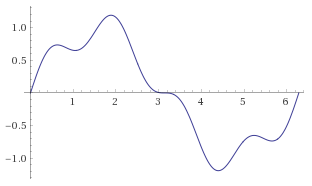
\includegraphics[width=\vismWdPercent{80}]{img/Screen-Shot-2018-06-13-at-11.08.30-AM.png}\end{center}

                You have my sympathy. The x-axis is the jhanas and subjhanas, from 1.1 to 4.4, or 1.1.1 to 4.4.4 if you want to go into subsubjhanas (which would involve adding 0.0625sin(16x) to the above equation). Unfortunately, what goes on the y-axis could be the subject of a book longer than this one and would read like the most difficult works of Aleister Crowley, but simple points are made here shortly with graphs included that hopefully you will find much more practical than esoteric.

                The possible complexity of this model is endless and it is no substitute for practice. Try not to become an arrogant twit like I did when I began to figure all this stuff out. Esoteric map theory won’t win you any friends or enhance your loving-kindness, and its benefits for finally figuring out the key points of insight practice are questionable at best.

                I have spent way too much time thinking about the fractals and modeling in my own practice. In my insecure moments, I have considered showing off and writing a book that detailed the hundreds of little parallels and patterns that I have noticed over the years, how this tiny little stage of some vipassana subjhana mirrored or was an inversion of another aspect of some other little stage of some other subsubjhana, but I couldn’t come up with any practical use for it at all. If you do the technique, you may see all of this and more. If not, reading about it won’t help you. On the other hand, if you are built like me, really like this stuff, and can use it to investigate the fine points of reality, then perhaps this will validate and resonate with your explorations.

                You don’t need this at all to see the true nature of the experience field, as that is more fundamental than these specifics. On the other hand, traditions such as Kabbalah (however you spell it) seem to have made related complex permutations into meditation itself. Those who are particularly inclined to complex analysis might want to try taking it as a vehicle for going beyond it. Also, guess where the complex geometric Tibetan mandalas that are supposed to be representations of enlightened awareness and its universe come from? Bingo!

                All that said, I did strip all the complex theory down to come up with a series of images that highlight some of the simple, practical points that come from deep, fractal-based map theory, and here they are. The graphs basically use an arbitrary −4 to +4 scale to give a general sense of how that aspect (such as need for sleep or level of motivation) might be in each stage. Individual variation is normal. You will notice a few oddities that are peculiar to me. For example, that I find Fear somewhat pleasant is likely anomalous and likely an artifact of me being an adrenaline junkie. Many may not experience everything the way these diagrams show it, but still they may have some general applicability.

                \begin{center}\includegraphics[width=\vismWdPercent{80}]{img/Ñanas-and-Motivation.jpg}\end{center}

                I begin with an easy one: the relationship between stages and general level of motivation to practice. In Mind and Body the mind is generally bright and we are excited. In Cause and Effect things are just odd in a neutral sort of way. The Three Characteristics stage tends to involve lots of pain, which can be demotivating. The A\&P is generally awesome, the peak of inspiration to practice for positive reasons. In Dissolution, we feel like couch potatoes, so our motivation is low. Fear helps our motivation a bit, but by itself can be disconcerting for many. Misery is about the same. However, in Disgust and Desire for Deliverance, we can suddenly be motivated, but this time for more aversive, renunciate reasons, and reasons related to a deep existential angst for awakening or release. Re-observation is one of the hardest stages, and motivation to practice can be at an all-time low. Equanimity helps, but often it involves somewhat low motivation to practice, as everything may seem too nice to need to do much of anything.

                \begin{center}\includegraphics[width=\vismWdPercent{80}]{img/Ñanas-and-Sleep.jpg}\end{center}

                Need for sleep tends to increase in the Three Characteristics, mostly due to how tiring pain can be. Sleep need can drop dramatically in the stage of the A\&P, suddenly peak in Dissolution, drop a bit again in Fear as our energy returns, and increase during the Dark Night, mostly due to how mentally fatiguing that stage can be.

                \begin{center}\includegraphics[width=\vismWdPercent{80}]{img/Ñanas-and-Body-Temperature.jpg}\end{center}

                The degree to which we feel hot or cold in our bodies also varies by stages. This body temperature variation can also relate to the tendency to perspire. As the early stages build to the A\&P, our sense of body heat increases. It drops a lot in Dissolution, and we may suddenly feel colder than we did just one stage before. We may sweat a bit more in Fear. It tends to increase a bit due to the struggle of Re-observation.

                \begin{center}\includegraphics[width=\vismWdPercent{80}]{img/Ñanas-and-Central-Clarity-1.jpg}\end{center}

                The degree to which we clearly perceive sensations at the center of our attention becomes more developed as we move up the early ñanas, peaks at the A\&P, drops suddenly as we shift into the third jhana and Dissolution, increases just a bit as the energy comes back in Fear and Disgust, plummets again in Re-observation, and increases in Equanimity, though not to the degree that it was present in the A\&P, oddly enough.

                \begin{center}\includegraphics[width=\vismWdPercent{80}]{img/Ñana-and-Clarity-of-Periphery.jpg}\end{center}

                The intensity of clarity regarding the periphery of attention, on the other hand, is only somewhat developed in the early stages, drops off again in Dissolution, peaks in the Dark Night stages, culminating in Re-observation, oddly enough, and drops a bit in Equanimity, whose balance across all aspects of attention is more pronounced, thus losing a bit of clarity in each area.

                \begin{center}\includegraphics[width=\vismWdPercent{80}]{img/Ñanas-and-Mind-Speed.jpg}\end{center}

                The speed of our minds increases dramatically in the early stages of insight, peaks in the A\&P, drops dramatically in Dissolution, ramps up again in Fear, drops back in Misery, peaks again in Re-observation but mostly around the periphery, and oddly is back to what feels like near-baseline in Equanimity, whose strengths are more integrative, accepting, and flowy than rapid-fire analysis.

                \begin{center}\includegraphics[width=\vismWdPercent{80}]{img/Ñanas-and-Energetic-Phenomena.jpg}\end{center}

                Energetic phenomena, often referred to as kundalini phenomena, begin in Cause and Effect, peak in the A\&P, drop off dramatically in Dissolution, may increase a bit in Fear, drop off for most of the Dark Night, may occur a bit in Re-observation, and are generally not happening in Equanimity.

                \begin{center}\includegraphics[width=\vismWdPercent{80}]{img/Ñana-and-Pain-Pleasure.jpg}\end{center}

                The degree of pain and pleasure (\emph{vedana}) we generally experience in our bodies also varies by stages. In Mind and Body our body tends to feel good. Shortly thereafter, in Three Characteristics, it often feels tense and painful. The A\&P is typically the peak of pleasure, insight stage–wise, being second jhana-based. Dissolution also feels good, but in a much more relaxed way. Fear generally doesn’t involve much pain, and the physical feeling of our body in Fear is typically slightly pleasant in the thrills and chills if we can notice this. Pain returns as the Dark Night progresses, and our body and mind may feel progressively worse as the restlessness and irritation at phenomena in general peak in Re-observation. The edgy, restless, irritating pain of Re-observation tends to differ in quality from the hard, stiff pain of the state of the Three Characteristics. Equanimity may involve mild pain, but there is also something nice about the neutrality of body feel we can notice in Equanimity, so I give it a slightly positive rating.

                \begin{center}\includegraphics[width=\vismWdPercent{80}]{img/Ñanas-and-Powers.jpg}\end{center}

                The stages most prone to spontaneous powers are the A\&P and Equanimity. They are very unlikely in the Dark Night and the least likely in Re-observation unless we have unusually strong concentration skills or a strong natural inclination in that direction. Some propensity to powers may return in Equanimity, but the motivation for them often drops off, thus partially modulating this stage’s remarkable powers potential.

                \begin{center}\includegraphics[width=\vismWdPercent{80}]{img/Ñanas-and-Mental-Illness.jpg}\end{center}

                Certain stages are more prone to reducing or exacerbating tendencies to mental illness. Mind and Body, as it provides a clear space around thoughts, tends to make people saner, and for this reason really helps with psychological work. The A\&P is distinctly prone to exacerbating manic phases, grandiosity, and moments of agitated psychosis. Dissolution is so chill that mental illness again becomes less likely, though it does have demotivating elements. The Dark Night is well-known to possibly exacerbate depression, social isolation, schizoid tendencies, and anxiety. Re-observation is the peak of the risk for mental illness, particularly regarding paranoia, psychosis, and suicidal ideation. Equanimity tends to reduce mental illness tendencies, given its open spaciousness and general sense of well-being.

                \begin{center}\includegraphics[width=\vismWdPercent{80}]{img/Ñana-and-Attention-Phase-Harmony.jpg}\end{center}

                Attention phase harmony is a hard thing to explain unless you are adept at noticing the degree to which phenomena and attention seem to be in synchrony. This quality peaks in Mind and Body, the A\&P, and Equanimity, which are generally also the least unpleasant stages and the closest to their shamatha jhana counterparts. It is at its worst in Re-obsevation, but can also feel moderately off in Three Characteristics. Dissolution is an oddity, in that it has good phase harmony, but I put it as neutral since most people don’t notice this at all, given the nature of Dissolution. Attention phase harmony also correlates well with where the shamatha jhanas and stages of insight are the closest, and Dissolution is the closest insight stage to the third shamatha jhana.
            \section{U Pandita’s Model}

                Sayadaw U Pandita was one of the greatest contemporary masters of meditation in the Burmese Theravada tradition (see his book \emph{In This Very Life}). Though he helped to train Bill and a few other people who helped train me, U Pandita’s models don’t quite agree with those of Bill and myself about how the ñanas and jhana line up. I thought that, in the interest of fairness and the inherent value in engaging multiple perspectives, I would present his model. In it, as in Bill’s, the first three stages of Mind and Body, Cause and Effect, and Three Characteristics all fall within the first vipassana jhana. However, U Pandita divides the A\&P into two jhanas, with the immature phase (when the meditator is still in the grip of the ten corruptions of insight) corresponding to the second jhana and the mature phase (when the meditator sees the true nature of the ten corruptions of insight and crosses the A\&P Event) as the third jhana. Everything from Dissolution to Equanimity then falls into the fourth jhana in his model. This does accommodate the vague formless experiences that can happen in Dissolution, as the formless realms come out of the fourth jhana.

                The problem I see with this map is like the problem with the other maps, namely, that some of the stages of insight tend to suck and the shamatha or pure concentration jhanas are usually pleasant or peaceful. Thus, to say that the Dark Night stages such as Disgust are part of the fourth jhana just rubs me the wrong way somehow, as does saying that Three Characteristics (which also tend to suck a bit) is part of the pleasant first jhana. Further, Dissolution is oh-so-close to the third shamatha jhana, and it is very easy to shift the one into the other and back again. The same is true of the A\&P and the second shamatha jhana. The point is that no matter how you slice it, the correlations are not quite perfect, and insight practice is rarely as pleasant as good old concentration practices. That said, there is something to these models anyway, and if you master insight and concentration practices and know a bit of theory, you will see for yourself what they were trying to get at, so get to it!
            \section{One More Model}

                The last model is one that is hinted at by a line in the \emph{Visuddhimagga} that says that Desire for Deliverance, Re-observation, and Equanimity are one.\footnote{\vismAssertFootnoteCounter{X}\emph{Visuddhimagga}, \href{https://edhamma.github.io/xref/?book=vism&ref=XXI.79}{XXI, 79}–\href{https://edhamma.github.io/xref/?book=vism&ref=XXI.82}{82}.} This cryptic phrase may be interpreted various ways, one being that the content of these three stages is likely to be largely the same, while the relationship to the content may change dramatically. It could also be used as justification for a third model that puts these three together in the fourth jhana. Further, as the fourth vipassana jhana is about equanimity concerning formations, we might presume that we would have had to perceive formations at an earlier stage, such as at the previous two, to have had the necessary time and experience to come to equanimity regarding them.

                Go see for yourself and consider which of these three models presented here fits with your actual experience, or throw this book and its models out the window and investigate the three characteristics precisely, regardless of what happens. Such decisions might be better made after reading the next chapter.
        \chapter[How the Maps Help]{How the Maps Help}

            Now that I have presented the maps of the progress of insight and of the vipassana jhanas, I will reiterate a bit about how they help and why I went to all that trouble. I will try to do this in chronological sequence and tie it in with what has been said in Part One. (Remember Part One? I hope so.)

            The maps tell you clearly what you are looking for and explain precisely why you are looking for it, how that insight helps, and how that insight provides the ground for what follows. The same thing could be said of the concentration state maps. If the stages of insight didn’t tend to bring up all sorts of unusual raptures and produce such a wide range of potentially destabilizing emotional side effects, there would not be so much need for the maps. You could simply tell people to increase their perceptual abilities until they awakened, and they would likely have few difficulties in doing so by properly applying the techniques. However, the insight stages do tend to cause these sorts of effects, so the maps are very useful for keeping people on track in the face of them.

            Remember the chapter called “The Seven Factors of Awakening” when I mentioned that the first factor was mindfulness and that this was really good for sorting out what is mind and what is body and when each is and isn’t there? That is because the first insight you are looking for, the one that allows you to see more deeply, is stage one: Mind and Body. Get it? This stuff is not random or arbitrary. It is all clearly laid out in a way that helps and fits with reality. In other words, the order is significant and worth respecting.

            Remember how I said in that chapter that we should try to experience the intentions that precede actions and thoughts, as well as the mental impression or “consciousness” that follows all sensations? That is the key understanding in stage two: Cause and Effect. Thus, mindfulness is the first factor of awakening because it leads directly to the first two classic insights into the truth of what is going on. If you want insight into something, then looking precisely into that aspect of things is the best way to acquire that insight.

            Once we have directly experienced these two insights, then the three characteristics begin to become obvious in stage three, which is exactly why the next factor of awakening is called investigation of the truth, i.e. Three Characteristics. The seven factors of awakening and the insight maps tell you exactly what you are trying to understand and why. You will not be able to directly understand the three characteristics without first being able to distinguish what is mind and what is body and the relationships between them. Without understanding the three characteristics, regardless of what you call them, you will not be able to advance. The Buddha laid it all out step by step. While this may seem unromantic, unpoetic, uncreative, and even dry, it is also extremely practical and without a doubt the clearest presentation of exactly how to wake up that I have ever seen presented in any spiritual system, just so my biases are made perfectly clear. In short, these maps and techniques can be \emph{profoundly empowering}.

            Once the three characteristics become clear, the mind naturally speeds up and becomes more powerful. This is because it finally begins to draw on its tremendous power to see things directly and investigate without processing them through thought. Anyone who has driven a car, played a video game, or done just about anything else, knows that you just do it, but if you try to think about every little thing you are doing, the action would be impossible.

            This increase in mental power due to non-conceptual and direct experience is related to the third factor of awakening, energy. Energy may now even be blazing up and down the spinal cord, the mind gets bright and alert, and soon energy is flowing naturally, as we begin to enter the early part of stage four: Arising and Passing Away. Remember how this correlates with the second shamatha jhana, where applied and sustained attention or effort are no longer needed? They just happen on their own, to a large extent, and energy is naturally present. Thus, it all ties together.

            The next factor of awakening is joy or rapture, which comes to predominate in the second vipassana jhana and the Arising and Passing Away, just as it does in the second shamatha jhana. Thus, all the important advice about rapture given earlier applies to the insight maps in Part Four. We are generally advised to avoid becoming a rapture- or kundalini-junkie in this stage, although I suppose that if this is your primary reason for meditating, it is certainly your right to do so. Just be wary of the inevitable crash.

            During the mature Arising and Passing Away, as well as in Dissolution (stage five), tranquility becomes important and more pronounced, but then becomes too strong in late Dissolution. Thus, it becomes important to build the sixth factor of awakening, concentration, and developing concentration is an oft-recommended strategy in the Dark Night.

            Finally, when the Dark Night really kicks in, as it will once we can again find our objects and stay with them (Fear through Re-observation), then Equanimity in the face of all experience becomes vital for progress, as stated in Part One. Thus, Equanimity can arise and Path can be attained.

            As mentioned before, the maps fill in the seemingly huge, frustrating, and nebulous gap from doing something like sitting on a cushion paying attention to the sensations of your breath and finally awakening.

            The maps also tell you exactly what the common traps and temptations of each stage are. They warn people about not getting stuck in Mind and Body by solidifying it into a jhanic state, which it closely resembles. They provide comfort and explanation when things might get jerky, unpleasant, or even downright painful in stage three, Three Characteristics. They admonish people not to get too fascinated with how much of a mighty meditator they might feel like in stage four, Arising and Passing Away, and even to examine the sensations that make up the seemingly wondrous and tantalizing corruptions of insight such as equanimity and rapture. They warn of the possibility of thinking that we are enlightened when going though that stage, as well as saying that it is normal for wild and sometimes explosive experiences to occur.

            I spoke with a friend who basically wanted me to help him rationalize that his recent A\&P experiences occasionally allowed him to touch High Equanimity. My advice was that a much more helpful form of inquiry would be to notice the sensations of fascination with this issue and notice the sensations of the rest of his sensate universe come and go moment to moment. If he couldn’t manage this, he should be putting his time into trying to figure out how to get together enough money and vacation time to do another long retreat and/or how to increase his daily practice time and the thoroughness of his investigation.

            The maps clearly state that the process is not a particularly linear one, and that after the highs of the Arising and Passing Away there usually follow times of difficulty when all the spectacular power of the mind and pleasure of meditation gained in the Arising and Passing Away are likely to fade dramatically. They warn of the numerous difficulties that may be encountered in the Dark Night stages, as well as provide lots of information about how to deal with them. The most common mistake is failing to investigate the truth of sensations deemed undesirable or unpleasant. It is hard to get on more intimate terms with reality when we feel a bit too emotional, vulnerable, raw, openhearted, or shaken, and so progress through the insight stages that make up the Dark Night is not always easy.

            While I do generally wish to avoid biting the hands that have fed me, I must say that not telling practitioners about this territory from the beginning to give them a heads-up as to what might happen is so extremely irresponsible and negligent that I just want to spit and scream at those who perpetuate this warped culture of secrecy. While many teachers may not do so because they don’t think many people will ever get this far, that in and of itself is a scary assumption that should cause some serious questioning of their teaching methods, techniques, and perhaps even motivations.

            Imagine that there is a medication called Damnital that is used to treat some form of suffering (perhaps it’s a pain medicine or an antidepressant). However, in a subset of patients its long-term use is known to cause pronounced anxiety, paranoia, depression, apathy, micro-psychotic episodes, a pervasive sense of primal frustration, pronounced lack of perspective on relationships, reduced libido, feelings of dissatisfaction with worldly affairs, and exacerbation of personality disorders, all of which can lead to markedly reduced social and occupational functioning. Imagine that these side effects are known to persist sometimes months and even years after someone stops taking the medication, with occasional flare-ups and relapses, with the only effective treatment being to restart the meds, perhaps increase the dose, add supportive care and counseling, and hope that these side effects pass quickly with little damage.

            Now, imagine that you are living in the dark days of paternalistic medicine during which doctors prescribe these practices without fully disclosing the potential side effects despite being fully aware of them. Imagine that drug companies are not required to disclose known side effects. Does anything in this scenario make you even a bit uncomfortable? I should hope so!

            Let’s say for the sake of argument that I am a fanatic who is blowing this way out of proportion. Let’s assume that Damnital only causes these effects in one out of every ten thousand patients. Would you have these side effects included on the little piece of paper that comes in the bottle? Let’s say it’s one in a hundred? At what point does it become absurd that those doctors and drug companies are being allowed to get away with this? Unfortunately, I must admit that I do not know the exact odds of these side effects happening to you. I do know firsthand that they happen and that if you cross the A\&P you are likely to run into at least some of them.

            These side effects are no fantasy. When they show up they are as real and powerful as if some dangerous drug had seriously skewed your neurochemistry, and I often wonder if that might be something like what happens. Thus, it seems only fair to have the same standards that we apply with such pronounced zeal and fervent litigation to drug companies and doctors also apply to meditation teachers and dharma books. For reasons unknown to me, this book is the first one I know of to spell out all of these things explicitly in language that everyone should be able to understand so that you can go into meditation having been fully informed of the risks and benefits and thus make informed decisions about your own practice. In the spirit of professionalism, I call on others who promote the dharma to immediately adopt a similarly high standard of open disclosure of risks, benefits, and alternatives for their own work.

            These maps point out that people might get stuck for a little while in Equanimity if they do not investigate even the sensations that make up equanimity, peace, relief, space, ease, clarity, expectation, confidence, and so on. The models (presented later) also go into detail about what does and does not actually happen at each stage of awakening, though this aspect of the maps is much more controversial than the maps of the progress of insight.

            Thus, the maps at their best inform the meditator in clear and systematic ways exactly what to do, what to look for, why, and exactly how not to screw up at each stage. They are no substitute for clear practice and investigation of the sensations that make up our experience, and they are poor aids for those who refuse to heed them and follow their advice. As I keep repeating, they can also be used as a basis for useless and even harmful competition between gung-ho meditators with insecurity issues and insufficient training in morality. It can and has been argued convincingly that we certainly don’t need to know these maps at all if we practice well. Despite the dangers of competition and hyper-intellectualization, the maps still have tremendous value when used as they were intended to be used. Still, give a poor rice farmer basic vipassana instructions and watch them practice well, gain insights, and run rings around some affluent intellectual westerner with the maps who can’t follow basic instructions and instead hyper-analyzes everything but the sensate phenomena they are supposed to be investigating. Just sayin’.

            One other very valid criticism of the maps, as I mentioned already, is that people are often very susceptible to suggestion, called “scripting”. Describing these stages can cause people to report having experienced something that resembles what the maps describe. Bill Hamilton’s favorite example was that if you mentioned that some stages of meditation involved an itch in our elbow (there is no stage I know of that does, by the way), then suddenly everyone would start reporting lots of elbow itching. The part of the maps that deals with emotional side effects is notorious for causing this kind of mimicry. For example, it is basically impossible to sort out what is just fear and what is insight stage six, Fear, based upon the presence of fear alone, as fear is a very common emotion. The aspect of the maps that deals with unusual raptures (both physical and mental) is less suggestible and is a more reliable indicator of the stage of practice.

            However, the fundamental increases and shifts in perceptual thresholds are extremely hard to fake, particularly if you have access to a map that goes into the extensive details presented here. Shifts in perceptual thresholds are the most reliable markers on the path of insight, the Gold Standard by which these stages are defined. For example, if you recently saw very fine vibrations that changed frequency with the breath, then had a big zap-through, spaced out for a while, now feel paranoid, and notice some relatively steady shamanic drum–beat like pulse that quickly leads to chaotic, edgy vibrations with complex harmonics, that’s very likely the insight stage of Fear.

            Thus, increasing our perceptual thresholds in terms of speed, consistency, and inclusiveness should always be the focus of our insight practices. Skilled teachers who use and are very good with these maps will consider all three—that is, emotions, raptures, perceptual abilities, along with the patterns relating to these that have unfolded previously—and use these to arrive at an educated guess as to what is going on with a student. With years of experience, we may eventually get good at doing this for ourselves. I have found that my guesses about my own practice are usually more accurate after I have had a year or two to reflect on what occurred.

            I will tell some stories later about how some of the maps made a huge difference in my practice and how other maps caused trouble. I am a firm believer that if there is enough good information out there, then it doesn’t have to be so hard for those that follow. Thus, I present these maps in the hope that they will help people to at least have some framework to understand the many and varied parts of the path. It is not that everyone uses maps well, that everyone will benefit from map theory, or that everone’s practice will fit the maps well enough to have them add value but, in general terms, I find that practice with maps is better than without them, and plenty of others have relied on them for thousands of years.

            Further, as absurd as this may sound to some, the maps allow you to plan your spiritual path to some degree. True, there are ultimate points of view that would make this perspective seem quite ridiculous, but indulge me. A sample plan might be like this.

            Go on a three-week retreat and really power the mindfulness and investigation all day long, consistently stretching your perceptual threshold and rate of investigation to its limits to maximize the chances of crossing the A\&P. It is not that hard to cross the A\&P even with imbalanced effort, so don’t worry about it. Remember not to be freaked out by the strange raptures around the A\&P. Note, a two- to three-month retreat would give you a great shot at stream entry if you are ready to practice and able to follow simple instructions, so if you are at that level, go for it.

            Once you have crossed the A\&P, Dark Night stuff will come bubbling up soon enough, and the choice to deal with this on or off-retreat will depend upon how much time you can devote to retreats and how much intensity you can stand. My vote tends to be for retreat if you can take the heat, but not everyone can the first time around and not everyone can easily spare the time. On the other hand, that Dark Night might just be a cakewalk for you. Give it a go and find out! In the Mahasi Sayadaw tradition, they typically think that two to three months of diligent noting practice on intensive retreat is enough to get many people to stream entry, but perhaps you do not have the time or dedication to step to that level yet, or perhaps you will beat the odds and just be with what is happening, settle in to your experience, and nail it.

            If you decide to deal with the Dark Night off-retreat, realize that you will likely fall back, but keep practicing an hour or two each day. Do your very best to realize that any of the odd feelings that you may experience are probably just Dark Night side effects. Try to imitate normal life as best you can and avoid rash decisions such as sudden and difficult-to-reverse renunciation of things you will want later. Try to be good to people and do your very best to keep your “stuff” from bleeding onto those around you. Find ways to honor and deal with your stuff that don’t involve projecting it out onto other people or making a mess of your life.

            If on retreat, or the next time you can go on retreat, just keep practicing as consistently and accurately as you can and avoid indulging in the content of your stuff at all costs. Put worldly concerns behind you for that period and investigate bare sensations with acceptance and courage.

            Practice equanimity regarding whatever arises, but be wary of indifference or apathy. This is not always as easy as it sounds, but for some it could be strangely easy nonetheless. Once the weight lifts, just keep sitting or walking or whatever, with no sense of special effort, but keep up gentle, ordinary, and consistent attention to the open, flowing field of awareness, with gentle emphasis on the three characteristics of the full field of experience, of space and what is in it. After really getting into High Equanimity, stream entry should arise soon enough; if it doesn’t, repeat the above until it does.

            From this point, you are “in there”, and progress of some kind is now inevitable. This first fingerhold on ultimate reality is extremely important, as without it you can wander far and wide and get nowhere. Advice for what to do next is given later.

            In this way of thinking, there are only about five stages, and they are relatively easy to identify. The first is before you get any sort of strong concentration, and the advice is to get your momentary concentration stronger through good, present-centered insight technique. The second is the first vipassana jhana, which involves staying with your objects, getting faster and more precise, and working through basic hindrances. The third is when things get cooking, the A\&P, the second vipassana jhana, which is usually obvious. The fourth is the Dark Night, which is also usually obvious. The fifth is Equanimity, which though usually obvious, can be confused with the A\&P. The instructions basically are to continue practicing with some awareness of the standard traps of each stage, and let your attention get broader as each new jhana requires. Memorize this basic five-stage framework and the standard advice for each basic stage, and you will be a stronger, more independent, competent, and empowered practitioner.
        \chapter[Beyond First Path (“What Next?”)]{Beyond First Path (“What Next?”)}

            I t can be easy for meditators to think they have completed a full cycle of insight and gotten stream entry when in fact they have not. It is also possible for meditators to have completed a cycle of insight and yet think otherwise, but this is much less common, at least in traditions that have good maps and in practitioners who have good dharma friends with whom to discuss their practice. Sometimes practitioners will be correct in thinking that they have achieved what they believe and say they have, but their friends and teachers may remain unconvinced. At times, a teacher or friend may think that the student has done it and yet be wrong. Regardless, just keep practicing and see what happens. This is the most fundamental principle for all these stages. A particularly useful and traditional guideline is to wait a year and a day before completely making up your mind. This is slippery stuff sometimes, and many states and stages can easily fool a practitioner, friend, or teacher into thinking that they are something they are not, as has happened to me more times than I can count.

            When meditators successfully complete their first cycle of insight, they have permanently debunked certain illusions to some degree, but many remain. Those that remain tend to include a new fascination with the understanding that has arisen from that path. However, if our “awakening” doesn’t endure the test of time, or if there is not a fundamental and sustained reduction in suffering, write it off and keep going. Even if we do complete a full cycle of insight, it is easy initially to imagine that more has been debunked than actually has been, so continue to practice training in morality throughout your life, as before, to avoid being bitten by the unskillful potentials that remain but are often hidden in the form of our own blindspots. Strangely, the internal obstacles that can tempt us to screw up become more subtle and seductive as practice deepens. These temptations tend to be at their worst during the next new Arising and Passing Away or during the next Re-observation.

            An extended series of progressions (cycles) of insight tends to proceed as follows. They may be called “paths” in the Theravada and “bhumis” in the Tibetan system, though there are some problems that arise in trying to resolve the inconsistencies in these two models that will be touched on a bit later. Thus, a more general treatment follows, and the descriptions of the stages here are not taken directly from any specific tradition but are influenced by a number of them. From one angle, none of this is necessary information, as continued practice just as before will move things along quite naturally. From another angle, this information might be useful if we have expectations of what might come next that are not in accord with reality, or that interfere with practice.

            Meditators can master this stage of awakening by continued practice as before. Stronger practitioners in Review can quickly learn to move through all the stages, starting from the Arising and Passing Away, through the Dark Night, up to Equanimity and possibly Fruition in a single sitting or even during some of the activities of daily life. Merely sitting down on a cushion, or being awake in the ordinary sense for that matter, will involve naturally moving through these Review cycles. The speed and clarity can vary widely depending on the practitioner, their specific practice, and other circumstances. We may even find it interesting to purposefully hang out in some of the stages of the Dark Night just to learn more from and about them, as they have very important lessons to teach and are very interesting territory. However impressive all this may seem, we may also come to realize that this is just a new beginning in some ways, like graduating from high school but then becoming a lowly freshman in college.

            The period after completing a cycle of insight and after gaining some strong sense of mastery of its stages is also a great time to work on concentration practice abilities. The reason for waiting is that concentration practices and insight practices tend to have inertia to them. If you have recently been trying to get into very stable shamatha states, this can sometimes make it harder for a while to see things flicker, although, after stream entry, there will always be some sort of flickering somewhere, as that is what stream entry does. Likewise, if you have recently been training hard to perceive flickering, it can be harder to get into very stable shamatha jhanas. Thus, what you don’t want to do is gunk up the natural mastery phase of your practice until you are comfortable enough with these stages to get stuck in one and not have it be a big deal. This usually takes at least a few weeks, but this is a very crude guideline, and everyone is different regarding timing. Judge for yourself how well you handle stages such as Re-observation and decide if you would be all right if you got stuck in it for a few hours.

            The time after gaining some mastery of these stages is also a great opportunity to work on our stuff. Doing concentration practices and working on our stuff go very well together, as mentioned elsewhere, since concentration states tend to bring our stuff to awareness more clearly so we can then work with it. The time during a mastery phase is also great for making sure that our daily life is functioning well, particularly if we made a mess of it while trying to become awakened or more awakened.

            Mastery of these stages tends to peak at some point, and the sense can arise that we definitely “got it”. For many, Fruitions tend to occur quickly, clearly, and easily—though again—not always. Given time and practice, we may begin to get bored with our current level of attainment and with our ability to attain these stages and Fruitions. Practice can begin to seem sloppy, and the quiet bliss wave after Fruitions can diminish unless we do not attain it for some longer period (which would probably require resolutions to that effect).

            The realization grows that there is more suffering still to uproot. We begin to see more layers of reality that are not well-understood or illuminated by our current understanding, hints of which probably revealed themselves very soon after attainment of that path. Subtle thoughts and mental patterns may be noticed at the edge of our perceptual threshold. Attention begins to incline towards the next level of reality that must be understood and away from familiar territory. More fresh insights begin to show up.

            We begin to investigate reality with more effort and clarity, as we did before, and so begins a new cycle of insight from the beginning: that is, access concentration, and then Mind and Body and the rest. This might play out as follows: soon after the sense of strong mastery, we will simply be meditating along, perhaps a Fruition will occur, and then suddenly the mind drops into this new state rather than a new review cycle beginning again. It is stable, interesting, and jhana-like. It is sort of like reinhabiting our life or reconnecting with the sense of the observer. It is also likely the next Mind and Body. This could also happen when we are just going about our day. Plenty may not notice it at all, as it can seem so ordinary and may feel very familiar.

            The postural obsession, odd movements, strange tensions and pains (second to third insight stages), emotional volatility, vibratory phenomena that seem new, a fresh and clearer sense of what dualistic perspectives remain, and all the other early progress of insight stuff may arise in its time naturally and perhaps sooner than we might wish. The phrase “leading onward” is often used to describe the wisdom that arises from dharma practice. Strangely, it is a phrase and a fact that I have cursed just as often as blessed, and entering new insight territory at inopportune times or before we feel ready reveals my reasons for this. Insight cycles can sometimes be traumatic, and it is often advisable to take a break to recover your sense of humor and appreciation of life before plunging on if you lost them along the way. However, at this point the dharma waits for no one and may propel you onward regardless of your wishes.

            Note well, for those in between stages, there is still the ability to easily attain any of the previous stages, starting at the level of the current Arising and Passing Away and moving up from there, so things can get quite murky when trying to figure out what stage we are in or attain specific new stages. It can be as if the early stages of the next large insight cycle are arising, whereas for a while practice always started out at the level of the Arising and Passing Away.

            Fixating on thoughts about what stage we are in is guaranteed to cause some degree of suffering that is worth investigating, especially in the in-between stages, though a gentle awareness of the maps can be useful if those sensations can be investigated. You might note “mapping, mapping” when thoughts of mapping arise. There can be a sort of fork in the path for a while, when the meditator is seemingly able to choose whether to review previous stages or press on. It can seem as though the background is solidifying and the mind is growing noisier as well as less predictable, less stable, and less skillful. More of our stuff may suddenly bubble to the surface. We may notice subtler thoughts and mental images, many of which we may wish we hadn’t. We may feel less “awakened”, as if our realization was fading. Clear and consistent insight practice, that is, understanding the three characteristics of all types of sensations, including thoughts regarding maps and goals, is the only thing that finally helps, just as before.

            After we cross the next A\&P, which may happen relatively quickly if we practice well and often, we will tend to have a very hard time re-attaining Fruition for a while, again assuming we were able to before. We may meditate along and then get stuck in a stage that seems to lead nowhere and is sort of like Low Equanimity, in that there are clear vibrations that are not varying with the breath or any other movement, and yet the background is too dense, noisy, and poorly perceived for clear and complete formations to show themselves.

            Finding the fork in the road back to familiar meditation territory can now be quite tricky, and even if we do find the way back, the old territory is unlikely to be particularly appealing. Fruitions may arise, but they may do so in a way that is less reliable or certain. Suddenly, we are “on the ride” again, and will soon have to face the fullness of the next Dark Night with all its implications. It may even be more challenging than before, but could just as easily be less so. One friend of mine sailed through one Dark Night in about six minutes, and the next one took him many years. There is no way to predict durations or degrees of difficulty of the next big cycle of insight.

            It can happen that many times we will try to meditate to Equanimity but fall back when we get to Re-observation. We may thus try to reattain previous stages, as we may feel that we are in over our heads. We may get into the next stage of Desire for Deliverance, wish very strongly to go beyond all of this, and do so by reattaining Fruition of the current path instead of attaining the next one.

            However, even if we can retreat into the old territory, we will still be haunted to some degree by the Dark Night in our lives and will have to learn to navigate skillfully in this territory one way or another. Sometimes re-mastering the current path—supported by resolutions to backtrack to Review—is helpful for building a sufficient foundation from which to proceed well into the new territory. Eventually, there is no way to go back, and we are simply left facing the new territory without an obvious skillful escape route.

            There can arise an odd phenomenon that Bill Hamilton referred to as “Twelfth Path”, though this phrase is not in common usage. It is, however, a common phenomenon for those who have attained at least stream entry and is probably the most important concept in this book for those working on the higher paths, particularly beyond second path.

            “Twelfth Path” is making a joke about the fact that there are at most four stages of enlightenment in the Theravada map and five to about seventeen (their path and bhumi counts vary by source) in the Mahayana and Vajrayana maps. However, it can easily seem that more brand-new and full-blown cycles of insight have been completed and yet there is still farther to go. If we are going to get obsessed with the fractal model that I mentioned earlier, it is likely to happen around here. Unfortunately, the fractal model is even more useless now than it was earlier, and so I strongly recommend avoiding it like the plague if you think you are in a new progress cycle rather than a review cycle. It is only by understanding the immediate moments that seem to make up the “fractal” that you will gain the understanding you seek, so, as suggested in the section “A Clear Goal”, keep your practice focused on the here and now, one part of which may be thoughts and sensations about fractals and maps.

            Things might proceed as follows. It seems certain that a cycle has been completed. Next, there seems to be a clear mastery stage that withstands the most rigorous tests, then more early progress of insight stuff shows up, the cycle begins to go around again, perhaps with more backsliding, moving forward, falling back again, remastering the old territory, more progress, and suffering shows up with its associated struggles and rationalizations. Then comes a sense of there being no option but progress and acceptance, and finally the sense that the cycle has completed itself. Soon enough there is a clear sense of a mastery stage, and so on. In this way, it may seem that some large number of paths have been attained, “twelve” in the joke, when in fact they have not. Or have they? Unfortunately, this is a tough question, and one that cannot easily be resolved.

            We may think that we are now at a higher stage of realization that is clearly different from before, but the “magic numbers” four, five, ten, or however many stages of awakening you think there are, simply may not seem to apply to our journey. It can also happen that, with increased clarity and progressive deepening of our practice, distinct progress of insight patterns may seem to be repeating within each of the smaller units of the larger pattern of the progress of insight, very much in the way of fractals, as detailed earlier. Beware! Do not get fooled into identifying with these idealized stages as actually being “where you are”. Fresh, luminous, transient textures and colors of space occur on their own. That is all. Try to perceive that directly rather than imagine that there is some continuous entity with some merit badge.

            New progress cycles and their accompanying vagueness can be very confusing if we are fixated on models but are not aware that the in-between territory is nearly impossible to successfully map in real-time. We may sometimes feel that we have just gone through the larger progress of insight cycle when we may have gone through just a small part of it. We may begin to think we see first, second, third, and fourth vipassana jhana aspects of each of the four larger vipassana jhanas. We may even begin to see patterns like those of a full progress of insight within each of the stages of the larger progress of insight or even within parts of each stage. A similar observation can arise in concentration practice with the shamatha jhanas, but this tends not to be nearly as problematic or dramatic.

            I have concluded that fear, anxiety, confusion, indecision, and even certainty about these issues are clear markers of what needs to be investigated: that is, these sensate patterns of emotional phenomena themselves. Noting “fear”, “confusion”, “frustration”, “doubt”, and the like can be very skillful to help us develop a metacognitive awareness of those patterns until we can delve more deeply into the sensations that make them up. In this way, these aspects of suffering have become trusted friends, clear signposts, and red flags, as well as aspects of the goal, which is the path in the end. The more we realize that those very processes are it, those very sensations are it, the closer reality is to understanding itself. The closer reality is to understanding itself, the less fundamental suffering there is.

            Additionally, I have concluded that the best reason to take these detailed maps to this extreme is that eventually they become too cumbersome. Thus, eventually they can be laughed at, even after having made useful points, while leaving us with no option but to be with reality, one aspect of which is the sensations that make up thoughts about maps. We can learn to laugh at ourselves and our deep-seated but futile desire to simplify fresh patterns of sensations and solidify them into a sense of an attainment that “we” have, or believe that they are “ours”.

            On the darker side, when we are unable to laugh at our deluded attempts to fix or freeze a sense of what some illusory “we” has done or attained, the phenomenon of “Twelfth Path” and the complexity of the territory between paths can cause considerable doubt, pain, frustration, and cynicism, the flip side of which is narcissism or grandiosity. The more afraid we are of not making progress, the worse these sorts of feelings can become. The more we compare our practice to the misunderstood sensations that make up the sense of “others”, the more needless suffering arises. These sensation patterns must be investigated clearly and seen as they really are, as always.

            A long-term view is very helpful, particularly if it paradoxically takes the pressure off and thus helps us to settle into what is happening right now. It will often not be clear which event was actually the new A\&P or which event was really a new path until we have the benefit of a few more months or years of practice. We may experience many strange events, state shifts, insights, and profound openings, all of which can be very compelling for some period. However, there tend to be just a few of these memories that, on careful reflection, stand out in the mind as being significant and by which we can clearly mark permanent shifts in our fundamental relationship to life and the world.

            In the next part of this book, I will lay out some models of awakening that involve various numbers of shifts in understanding. We may be tempted, as I foolishly have been, to count the landmark events in our practice and try to correlate them with these models based purely on how many times they seem to have occurred. This is a set-up for trouble, so please learn from those of us who have done so the hard way, and do not try it, as tempting as counting paths can be. A vastly superior form of inquiry and investigation is to carefully examine anything that seems to involve a sense of a split, of a \emph{this} and a \emph{that}, particularly at the rate of one to ten times per second or even faster if you can pull it off. Which sensations seem to be the watcher, and which sensations seem to be watched? Try to see the true nature of these sensations one by one as they occur.

            It must be said that after three or four of what seem like complete insight cycles or paths it can take quite awhile to get a clear sense of what subtle dualities remain. You might find yourself walking around for days to months thinking, “Dang, I’ve really got it now. I’m just seeing it no matter what happens. Cool! I might have cracked the thing! Dude!”

            Give things time and beware of assuming you have attained more than you have. It is a \emph{very common} and embarrassing problem, especially because it often goes unrecognized, but those who are mature, honest, and familiar with this territory understand it well. However, those who do not know this territory may not be so forgiving, so beware of claiming a specific level of realization, particularly some “final” realization, however you define it, until you have carefully checked out how it performs in real-world tests for a very long time. I would advise thinking along the lines of, “Well, my working hypothesis is that it seems I have achieved whatever, but I will keep an open mind and be cautious in what I say and write.”

            Use the descriptions of the more reproducible of the models of realization that follow to give yourself a general sense of the territory and what tends to need work and investigation. Avoid whenever possible the traps mentioned here, but when you realize you have fallen into any of them, which is ever so human and common, accept it, learn from it, and laugh! Should you realize that you have failed to heed this advice, that you have bought into some limited definition of yourself as a realized being of some defined rank or level despite the warnings, you can try to deny it for a while, that’s okay. You can imagine that you are very sure you know “where you are”, as that sort of artificial solidification of reality is common enough. You can get pissed off at yourself, that’s normal. You can beat yourself up if you think that it will help, though it rarely does. You can get bitter, though such responses tend to wear out their welcome. You can pump yourself up, dwelling on “your” imagined or real successes, though this tends to ring hollow soon enough. You can try to pretend you don’t care what stage or level you have achieved, though eventually this gives itself away. However, when you feel you are done with these things, accept, learn, lighten up, and laugh! Repeat as necessary and then get back to investigating those sensations.

            All that said, for those who have made the mistake of making some claim they later realize is inaccurate, I offer the following from a post on the Dharma Overground, slightly edited:

            “The known problems with goal-oriented practice are many, with open disclosure and a culture of labels, stages, states, levels of attainment, and the like causing predictable benefits along with predictable trouble. The situation that comes to mind is as follows: We are all excited about practice. We practice hard and well, aiming for a very specific goal. We achieve something that, at the time, really feels like we have done it. We are not consciously trying to fool ourselves or anyone else, but just honestly feel we have attained whatever state, stage, realization, or transformation based on our best understanding of the criteria and our best internal (and possibly some external) assessment. We make the claim that we have done it. We receive whatever social benefits and downsides result from having made that claim. Time passes …

            Things begin to show up that clearly are not as well seen as we thought they were, not as transformed as we thought they were, and we begin to feel that we were wrong about what we had done. Assuming our new assessment that we were wrong is itself correct, which it isn’t always, the questions arise: Was I totally delusional? Am I a bad person? Was it just that, at that time, it really seemed to have been what I thought it was and anyone would have been fooled as I had been? Was it really that I had done that thing at that time, but that transformation of perception was not as irreversible as I thought it was? Could I have possibly known at the time that it wasn’t that attainment or that it wouldn’t last? These are hard questions to answer, but that is not really the important issue.

            Where the real problem comes is the let-down, the embarrassment, the shame, the strange role reversals we might find ourselves in if that attainment turned us into some sort of teacher, expert, or authority, the personal confusion about what is suddenly happening and why, the disappointment that comes when we worked so hard and things didn’t work out as we thought. All of that can cause the worst part of it all: isolation. If we find ourselves unwilling to admit to others that we were wrong, or feeling like we are unable to do so, or that we will be ridiculed, blamed, or ostracized if we reveal what we know to have not been true—then real damage is done, for it is in those times that we most benefit from friends who can help us put it back together, go back to basics, regroup, retool, or modify our practice, learn, grow, and move on.

            Instead, we may find ourselves feeling like outcasts, failures, victims of our own hubris, afraid of being thought of as liars, fools, or both. We may disconnect from our fellow dharma companions, communities, teachers, friends, family members, and wander lost and confused, which is something that very few handle well in the shadow of some feeling of past glory, achievement, and even widespread recognition and authority. That isolation is where the real damage happens.

            As one who has gone through lots of cycles over the years that led to lots of plateaus, many of which were quite impressive for some period but later faded or reality-tested at a lower level than first impressions seemed to indicate, I can totally empathize, as I have been there and done that and very well may do it again. It can be very painful and disorienting.

            Realize though that these challenges are not only going to happen, they are very normal in this open-disclosure world of states, stages, names of levels, and achievement-oriented culture. If we recognize this as a community and can encourage conversations about it, then when it happens, which it will and perhaps often, members of the community who are dealing with all the complexities that these strange phases can cause won’t have to deal with the additional stigma of feeling like people think we are freaks, losers, or knowing or unknowing charlatans when we face the likely outcome of blowing it and making some grand claim that didn’t turn out to hold up over time. We will also get to benefit from the reality testing and other benefits that good dharma companions provide.

            Those wise dharma companions who supported us through admitting to error also get the benefits of living in a culture and community that is realistic and kind, such that, when they make their own mistakes, they can stay connected and be helped also, and you may be surprised at how much people who make mistakes like this can grow to be amazing practitioners and wise beings later. Much can be learned from falling down, and hopefully we will be lucky enough to have good and kind people around to help pick us back up such that we can later do the same for them or others.

            Thus, I urge each of you, should you run into someone who has this happening to them, who has claimed something and then renounced that claim, to have similar empathy, to wish that person well, and to realize that, if you are in this rarified business long enough, it will likely happen to you. When it does, think about how you would want to be treated and pass that on ahead of time if you haven’t already been in their shoes, realizing that you might very well be soon enough. This is the mark of a mature community of practitioners and it leads to more healing, mutual respect, kindness, renewed progress, inspiration, and harmony than negative, defensive, condemning, demonizing, and other immature reactions, not particularly well guided by the morality, loving-kindness, and compassion that the Buddha advocated. Hopefully, by recognizing this potential shadow-side of gung-ho, technical, stage- and state-based meditation culture, we will be better prepared to handle it well when challenges arise.”

            Speaking of models, states, and stages, here are some more…
    
    \part[Awakening]{Awakening}
        \chapter[Models of the Stages of Awakening ⚡]{Models of the Stages of Awakening ⚡}

            Before I discuss the various models, I should begin by saying that this is almost certainly the most easily misconstrued chapter in this book. Further, if you are a big fan of standard Buddhist dogmas, I strongly recommend that you stop reading this chapter now and skip ahead to other sections of this book. Seriously, I’m about to get quite irreverent again, but in that irreverence are bits of wisdom regarding the models of awakening that are hard to find so explicitly stated elsewhere.

            In the ongoing “axes of development” theme, this chapter will discuss various beneficial perceptual and functional modifications and insights you can realize about the way reality manifests. I am also going to talk about a lot of the traditional models found in various forms of Buddhism, but before I do, I want to talk about models in general, particularly their general uses and problems. We have already seen a lot of this with the progress of insight, but it is more important in this chapter, as the progress of insight is in many ways very straightforward (in other ways not so much), but it is a wonder of straightforwardness in comparison with the models that deal with stages of what might be termed realization, enlightenment, awakening, etc., which have serious problems. While I am generally known as a “map guy”, I think that most of the maps of awakening are seriously problematic, and I find that only a few contain some degree of accuracy and have some degree of practical value.
            \section{General Problems with Current Models}

                I will get right to the point and list the major general problems with most of the standard models of awakening and then spend some time fleshing out the specifics.

                Some models assume predictable linear development, such that if you attain this, next you will attain that, and so on, with this and that being very specifically defined and always following an immutably linear path. I call this “the linear fallacy”. It is not that there aren’t some truths in these models, but there are generally problems as well, and all of the linear models I know of have possible exceptions that I have known of secondhand from my fellow dharma practitioners and some firsthand in myself.

                A related set of models are the models that assume there is only one true track along which people progress, usually defined by some specific dogmatic tradition, and these models generally either completely fail to acknowledge other models or disparage other models to some degree, making them more accurately “the one best and only track” models.

                Some models assume that if you attain or understand one thing, you will automatically attain or understand something else that might be entirely unrelated, something I call “the package fallacy”. A simple, classic example would be that if you understand the three characteristics of the sensations that make up your sensate world, you will also necessarily not be able to feel certain emotions or will always be a very pleasant person to be around. It is not that packages of abilities, transformations, and understandings don’t occur, as they sometimes do, but most package models presume it will always happen exactly that way or that the packages will always contain the same transformations or elements, when in fact for most of the standard packages there are variants and exceptions as they relate to what happens in real life. Said another way, the package models assume simultaneous, synchronized, guaranteed, perfectly predictable development along totally different axes of development.

                Some models assume that, if you can perceive or do something now, you will always be able to (at least until you die, that is, in models that don’t assume realizations carry on into a “next life”). I call this “the permanence fallacy”. It is not that there aren’t some very long-lasting and extremely resilient transformations that can occur, but some of the models that involve permanence have problems that I will touch on in a bit, with what happens when pratitioners have strokes and other health issues that can damage the brain representing the tip of the iceberg.

                Some models assume that if you attain something, you will automatically describe your attainments or experience in certain ways, such as using very specific terms or even very specific lists of descriptions. I call this “the descriptive fallacy”.

                In a similar vein, some models assume that if you attain something, you will automatically know that you have attained it, what it is called, what it is, what it does, and what it means, as well as all the capabilities it bestows. I call this “the perfect self-diagnosis fallacy”.

                Some models assume that there is only one endpoint that is valid, final, or ultimate, and that it will look a certain way, often a very specific way related to a very specific person and how they look or looked. I call this “the final destination fallacy” or, as Kenneth Folk calls it, ”pernicious convergence”, meaning the belief that all roads lead to some very specific final point if you take them all far enough. If you look at the lives of the most accomplished students of the Buddha during his lifetime, such as Sariputta, Dhammadinna, and Moggallana, you will notice that they were much more specialists than they were clones, each having their own skill sets they were particularly good at, their own personalities, their own styles of presentation and emphases.\footnote{\vismAssertFootnoteCounter{X}Definitely check out the remarkable book \href{https://www.wisdompubs.org/book/great-disciples-buddha}{\emph{Great Disciples of the Buddha, Their Lives, Their Works, Their Legacy}}, by Nyanaponika Thera and Hellmuth Hecker, edited by Bhikkhu Bodhi.} Thus, we shouldn’t expect practitioners today, who are often coming from significantly more diverse conditioning than those who studied with the Buddha, to be more homogenous than those early students were.

                It is worth noting that I have fallen victim to believing all these fallacies to some degree at some point, though now don’t completely accept any of them. Exactly how these fallacies do and don’t apply is complicated. The problem is that many of them do get at something that can and does happen or something that is at least partly true with some qualifiers at points. As I introduce the various models, I will try to point out which of them I feel fall into each of these various traps and to what degrees some of those traps may not actually be traps but contain some valid truths.
            \section{Models that are Mostly Unhelpful}

                Now I am going to present multiple models of awakening that I largely don’t like and I will explain why I don’t like each one as they come up. Most of these models are too simple and unsophisticated to detail the wide variety of what we naturally find in the wild jungle of meditators. We may of course forgive the various creators of these models for speaking out from the perspective of their own time, place, culture, practice, goals for developing the model, and limitations. I will assume they were all doing their best with what they had. Still, I care most about contemporary utility, so that is the filter I will apply when explaining and critiquing them.

                One major problem with most of these models is that we take this imagined something, this mental model, and project it or superimpose it onto our practice and then fixate on that mental construction of an ideal and attempt to imitate it rather than doing the practices that lead to the real deal, however defined. It is also very easy to use various models to script yourself into believing that you have accomplished what they are pointing to when in fact you have either done nothing of the kind, or accomplished part of the practice but left further possible depths of it entirely unexplored and unrealized. People can really get weird, stuck, and even totally flip out if they are using models that are too far out of touch with the circumstances within which they exist, and imitate an ideal that is not aligned with what is going on in their specific contexts and circumstances. I have seen more real-world examples of this happening than I care to count.

                Thus, my distinct preference when practicing and when motivation and discipline are sufficient to motivate real practice is to assume that “enlightenment” is completely impractical, produces changes that are very limited in scope, carefully defined, and circumscribed, and has nothing whatsoever to do with the scopes of the other two trainings of morality and concentration. This means that I take it as a working hypothesis that it will not make me a better person in any way, create any beneficial mental qualities, produce any states of happiness or peace, and provide no additional clarity into any of the issues concerning how to live my ordinary life. I have experimented with adopting other views and found that they nearly always get in the way of my insight practice, which is perceiving the sensations that occur now, however they are, as well as ideals about them, which are just more transient sensations. Thus, it is not that this particularly pragmatic view is entirely true, as it obviously isn’t, but it really does work well \emph{when practicing}, and practice that attains results is what I care about.

                It is not that I can’t appreciate the traditions that realize that, since insight can arise on any object or quality of reality, those qualities of arising reality might as well be skillful, as this is a reasonable perspective. For example, if you are visualizing a field of buddhas and bodhisattvas who project their good qualities into your mindstream while you also try to see the essential nature of this luminous display, that can clearly be skillful practice. It is not that we can’t operate on two fronts at once, that of insight and that of skillful content and profound meaning, and most people find themselves doing this in their practice anyway to some degree. However, as content is so tempting, and insight often so counterintuitive, many who try to do insight practices that also equally focus on specific qualities of content will stray far to the side of content and miss the insight aspects. So, I offer my perspective as a counterbalancing measure, not as some absolute injunction.

                Further, nearly all meditative practices and traditions are based at least to some degree on idealized views of how the specifics should be. Views so easily become reified, absolutized, and thus the temptation is to not investigate the sensations that make up thoughts about that view, but rather to imitate the ideal expressed in the content of that view. These traps are very easy for people to fall into. This attempt at imitative versus applied practice can seem so much like actual insight practice, but it is not. It is true that good outcomes and positive personal development can arise from this sort of practice, so it is not that I am criticizing those who focus primarily on positive qualities, meaning, and high ideals regarding the specifics their lives, but I am instead stating that many will miss what is more fundamental than these skillful emphases.

                I realize that I am probably not doing a good job of advertising awakening here, particularly following my descriptions of the Dark Night. \emph{MCTB1} stopped there and said basically, “Good point. My thesis is that those who must find it will, regardless of how it is advertised. As to the rest, well, what can be said? Am I doing a disservice by not selling it like nearly everyone else does? I don’t think so. If you want grand advertisements for enlightenment, there is a great reeking mountain of them there for you to partake of, so I hardly think that my bringing it down to earth is going to cause any harmful deficiency of glitz in the great spiritual marketplace.” However, my not advertising awakening much has caused enough complexity that I have included more about the benefits of practice despite my strong reservations about doing so.

                Bill Hamilton had a lot of great one-liners, but my favorite concerned insight practices and their fruits, of which he said, “Highly recommended; can’t tell you why.” It is traditional to advertise awakening or enlightenment in the negative in Buddhist and other traditions (for example, Christian contemplatives’ “via negativa”), either stating what it is not or stating what is lost at each stage. It is so very tempting to imagine that “freedom from suffering” will naturally translate into a fixed and unchanging state of mental happiness or peace, and this can tempt us to try to mimic that idealized state. That mimicking, in which we try to fix our mind on certain specific qualities that we privilege regardless of circumstances, would obviously be a concentration practice.

                Having said all that, the fact is that the models of the stages of awakening are out there and available. Even when they are not explicitly mentioned, they influence how people describe realization. Stronger practitioners routinely use various conceptual frameworks when engaged in the “shop talk” of meditation. Scientists are starting to try to figure out how to use various models to put people into categories that make for meaningful contrasting studies by various measures—from behavioral studies to studies using data collected with instruments such as fMRIs and EEGs—but unfortunately much of what they have to work with is far less than optimal. Thus, I have decided to try to work with some of the traditional problematic models so that they might be used in ways that help rather than harm. This is more difficult than you might think and, as reality testing with \emph{MCTB1} has shown, routinely backfires.

                There are days I wish the terminology for awakening didn’t exist, the models didn’t exist, and the whole process was largely unknown to the ordinary person so that it would be less mythologized and aggrandized, thereby making conversations about it more down-to-earth and less triggering. I wish we could start over, strip away all the mythical trappings and alienating cultural elements, create simple, clear terms, and move on. The longer I do this, the more I appreciate why some of my teachers wouldn’t talk about or use models at all in any explicit or defined way that I could tell, but I will bet, being humans with brains that can’t help but think in patterns and reductive terms, that they had models they used to evaluate students’ practices even if they didn’t credit those models.

                There are other days when I think that at least people know it might be possible, even if most of what has been said about it is pretty fantasy-based. My greatest dream is that the current generation of accomplished and semi-accomplished teachers will go far out of their way to correct the descriptive errors and false promises of the past and lay the groundwork for the perpetuation of these reforms despite the economic and social pressures to do otherwise. One of the issues restricting reform is that unfortunately only a few have gone far enough to see how the majority of the golden dreams of awakening do not hold up to reality testing, and most have not seen the true, deep, and amazing benefits of correct practice. Another thing holding this back is that putting oneself on an artificial pedestal based on promising false hopes and dreams can be rewarding in many ways. One way or another, the number of voices trying to bring things back in line with what can actually be done is miniscule compared to the forces that want to make it into something so grand and thus largely unattainable yet paradoxically quite marketable.

                Before I get too far into the details, I should explain that the most essential principle I wish to drive home is that \emph{this is it}, meaning that this moment’s sensations contain truth. Any model that tries to drive a wedge between the specifics of what is happening in your world right now and what awakening entails needs to be considered with great pragmatic skepticism. With the simple exception of clearly perceiving sensations occurring now and seeing through the illusion of a separate, continuous individual, nearly all remaining dreams related to awakening, however beautiful, are problematic to some degree. This basic principle of \emph{this is it} is essential to practice, as it focuses attention on the here and now, and happens to be true. Back to the complexities …

                The mental models we use when on the spiritual path can have a profound effect on our journey and its outcome. Most spiritual practitioners have never really done a hard-hitting look at their deepest beliefs and assumptions about what “awakening” or “enlightenment” means or what they imagine will be different when they “get enlightened”. Many probably have subconscious or largely unconscious psychodynamics and ideals that have come from sources as diverse as family dynamics, religious or non-religious upbringing, education or lack of it, cartoons, TV shows (\emph{Kung Fu} comes to mind), movies, legends, 1960s gurus, music, magazines, media of all sorts, and countless other aspects of pop culture and the cultural and temporal milieu of which we are the inevitable conditioned products. More formal and traditional sources include the ancient texts and traditions of Buddhism, Hinduism, Taoism, Sufism, Kabbalah, Christianity, Western mystical traditions (Alchemy, Theosophy, A∴A∴ and other Golden Dawn-related traditions, such as the various strains of Wicca, etc.), the ancient Greek mystery schools (including the fragmentary writings of those such as Heraclitus), and the non-affiliated or ambiguously affiliated teachers such as Kabir, Khalil Gibran, the Krishnamurtis (J. and U. G.), and many others.

                Modern fusion traditions, such as the various new versions of Buddhism and other traditions available in the West, also have a wide range of explicit and implicit ideals about awakening. Plenty of people also seem to take their personal higher ideals for themselves or for others that have arisen from hard-to-track sources and made these a part of their working, if usually poorly-defined or unidentified, models of enlightenment. There is also a strong tradition in the West of believing that awakening involves perfecting ourselves in some psychological sense, though this is also prominent in certain Eastern and traditional models as well in slightly different forms. This trend also makes attempts at the scientific study of these mental transformations very difficult, as just attempting to explain what has changed so often gets lost in large amounts of cultural baggage. This can color study design, implementation, and interpretation, and might be termed some sort of “unconscious ideals of enlightenment bias”.

                Just about all these sources contain aspects that at times may be useful and at other times not, even sending people in the wrong direction. It is hard not to be inspired by grand visions of how amazing we might become, chasing after the various archetypal masters’ legendary examples of excellence. Those extremely high ideals ring deep within our collective hearts and call us to find those qualities within ourselves. Thus, as a pragmatist, I have tried to strike some balance of presenting the good, the bad, and the ugly in a way that hopefully will work for my imagined readership. Here “work” means “facilitate results-producing practice”, and you as actual readers will have to figure out for yourselves whether any of my ways of presenting it does that. If not, you will have to figure out where you can find such practice, as it is entirely possible that my way of presenting this material may not work for you, or that it does not achieve that balance of reality-based models that yet speak to something deep in your own makeup and thus compel you to realize your own potential as a wise and compassionate person.

                To take on the models of the stages of awakening is a daunting task, but by breaking it down into simplified categories, some discussion of the mass of dogma of varying relevance and veracity is possible. The number of contradictions that can be found even within each specific tradition on the subject is much larger than I think most people imagine. For instance, those who attempt a systematic review of the dogmas of awakening within the Pali canon will find themselves tangled in a mass of widely divergent doctrines, myths, stories, and ideals, and this is only one tradition. Attempting to do this across the various Buddhist traditions leads to endless chaos, and attempting to do it across the rest of the world’s meditative traditions gets almost impossible, as the range of ideals out there is vast. I will use simple, broadly applicable models and discuss specific models that come from some of the more standard Buddhist traditions, and try to relate these to reality. In the end, relating them to reality or throwing them all out the window is part of the practice, and that falls to you. One of my favorite teachers was from a Thai Forest lineage and was at the very far end of the throw-the-maps-out-the-window school.

                I consider this attempt to make sense of the models to be just one addition to an old and ongoing tradition of attempting to reform the dogma and bring it back in line with verifiable truths, albeit one that is more specific and comprehensive than any that I have found. Each new culture, place, time, and situation seems to need to do this again and again, as the forces within us and society that work to promote models that are out of touch with the truth of things are powerful and perennial, with money, power, fame, ideals of endless bliss and pleasure, the enticing draw of the ideals of self-perfection, and the pernicious inertia of calcified or unquestioned tradition being chief among them.

                In that same vein, this chapter is very much a situation in which I explicitly claim a very high level of realization, write as if what I have achieved is sufficient authority to write a chapter such as this one, and then present it as if this is a definitive text on the subject, enough to contradict significant portions of 2,500 years of tradition and the teachings and writings of countless previous and current commentators. The previous versions of this book contained the line, “While it is hard from my current vantage point to not believe this to be true, anyone with sense will read this chapter with appropriate skepticism, and this, as I see it, is one of the strengths of properly applied Buddhism and rational thought in general.” That line needs revision, and explicit revision that compares it to the previous version. Here is something that I think is better than what I wrote before, and one day perhaps I will think this is wrong and write something else.

                From this current vantage point I see an extremely broad range of various beneficial mental modifications that people have managed to accomplish, and they do not all look the same. Some upgrades occur out of the standard sequence that I would typically expect. Some practitioners seem to skip steps and go straight to perceptual modifications and upgrades that have surprised me. Some have suddenly lost previously available abilities after they managed to accomplish some interesting shift. There are further complexities that I will try to touch on as we go. So, take these models with a grain of salt. They are models—and reality, particularly the reality of the mind and perception, is very, very complicated. I do think there are some essential truths that people can realize for themselves with a fair degree of predictability, but within that there is a whole lot of variability about the specifics.

                The Buddha asked people not to take his word at face value, but instead to do the experiment and see if they come to the same conclusions. I recommend the same. If you achieve something beyond what I state is possible, more power to you, and please let me know how you did it! I would feel real regret if this work in any way hindered another from achieving his or her fullest human potential. I am always looking for practices and concepts that are useful. While there is not much new under the sun, there are a few things on occasion that are, and if something you did worked to accomplish something beyond what is currently available and known, you should test it out for a while and, if it still performs as you think it does, let someone know.

                Finally, to the models … Here is a list of the basic categories of models that I use, though most traditions contain a mix of most or all of these. There are probably other aspects of the dreams of enlightenment that I have failed to address, but this list should cover most of the basic ones. I look at each of these as representing some axis of development, and basically all of them are good axes to work on regardless of what they have to do with enlightenment. That said, from what I have already written, it will not be hard to pick out my favorites. These are components that are typically put together to form more complex, traditional models, but looking at these specific parts of these compound models allows us to really get to the nitty-gritty of each of the more complex models.
                \begin{description}
                   \item[Non-Duality models:]  involve eliminating or seeing through the sense that there is a fundamentally separate and continuous centerpoint, agent, controller, watcher, doer, perceiver, subject, self, observer, or similar entity.
                   \item[Direct Perception models:]  involve removing or seeing through some distorting or interfering factor in the way we perceive sensate reality.
                   \item[Time and Space models:]  involve transforming some aspect of the way time and space are perceived and understood.
                   \item[Fundamental Perception models:]  involve directly perceiving fundamental aspects of things as they are, including perceiving emptiness, luminosity, impermanence, suffering, and other essential aspects of sensations regardless of what those sensations are.
                   \item[Specific Perception models:]  involve being able to perceive more and more, most, or all of the specific sensations that make up experience with greater and greater clarity during most or all times, and usually involve perfected, continuous, panoramic mindfulness or concentration at extremely high speed.
                   \item[Emotional models:]  involve perfecting the emotions, limiting the emotional range, usually involving eliminating things such as desire, greed, hatred, confusion, delusion, and the like, or eliminating emotions entirely.
                   \item[Action models:]  involve perfecting or limiting the things we can and can’t do in the ordinary sense, usually relating to always following some specific code of conduct or performing altruistic actions, or believing that everything we say or do will be exactly the right thing to have done in that situation.
                   \item[Powers models:]  involve gaining abilities, either ordinary or extraordinary (psychic powers).
                   \item[Energetic models:]  involve having the energy (chi, qi, prana, etc.) flowing through the energy channels in the proper way, the chakras spinning in the proper direction, clearing our aura, etc.
                   \item[Sleep models:]  involve changing aspects of sleep, such as how much we sleep, what happens in dreams, and being conscious while sleeping.
                   \item[Specific Knowledge models:]  involve gaining conceptual knowledge of facts and details about the specifics of reality, as contrasted with the models that deal with directly perceiving fundamental aspects of reality.
                   \item[Psychological models:]  involve becoming psychologically “perfected” or eliminating psychological issues and problems, i.e. having no “stuff” to deal with, no neuroses, no mental illnesses, having perfect personalities, etc.
                   \item[No-thought models:]  involve either limiting what thoughts can be thought, enhancing what thoughts can be thought, or reducing or stopping the process of thinking entirely.
                   \item[God models:]  involve perceiving or becoming one with “God”, or even becoming a god oneself.
                   \item[Unity models:]  involve becoming one with everything in some sense.
                   \item[Physical models:]  involve having or acquiring a perfected, hyper-healthy, or excellent physical body, such as having long earlobes, beautiful eyes, a yoga-butt, or super-fast fists of steel.
                   \item[Biological models:]  those that relate to the degree to which realization transforms our actual biochemical function.
                   \item[Radiance models:]  involve having a presence that is remarkable in some way, such as being unusually charismatic or radiating love, wisdom, or light.
                   \item[Karma models:]  involve becoming free of the laws of reality or the causes that make bad things happen to people, and thus living a blessed, protected, lucky, or disaster- and illness-free life, or perhaps creating no new conditions that could lead to any possible suffering for anyone.
                   \item[Perpetual bliss models:]  involve saying that enlightenment is a continuous state of happiness, bliss, or joy, the corollary of this being a state that is perpetually free from any form of pain. Related to this are models that involve a perpetual state of jhanic or meditative absorption.
                   \item[Concentration models:]  involve the various fruits of concentration practices and typically relate them to awakening in some way.
                   \item[Immortality models:]  involve living forever, usually in an amazing place (Heaven, Nirvana, a Pure Land, etc.) or in an enhanced state of ability (angels, bodhisattvas, sorcerers, etc.).
                   \item[Transcendence models:]  involve the idea that we will be free from or somehow above the trials of the world while yet being in the world, and thus live in a state of transcendence.
                   \item[Extinction models:]  involve getting off the wheel of suffering, the round of rebirths, etc., and thus never being reborn again—or even ceasing to exist in any way at the moment of enlightenment, that is, the great “poof!” on the cushion, not to be confused with the more mundane atmospheric consequences of a legume-based diet, as anyone who has been on a vegetarian meditation retreat knows all too well.
                   \item[Love models:]  involve us loving everyone and/or everyone loving us.
                   \item[Equanimity models:]  involve awakening being characterized by a perfect, pervasive, perpetual state of equanimity.
                   \item[No-preferences models:]  involve having no preferences, opinions, tastes, likes, or dislikes.
                   \item[Special models:]  involve us already being or becoming special.
                   \item[Social models:]  involve being accepted for what you may have attained, that you have attained something because people think you have, and variants on these themes.
                   \item[Ultimate reality and unreality models:]  involve adhering to specific positions about questions of Ultimate reality and unreality as they relate to awakening and the true nature of reality.
                   \item[Meaning models:]  involve advocating for an optimal set of values, goals, and meanings for practice, as well as the claim that awakening will result in a specific set of views regarding values, meanings, and the answers to key perennial questions.
                   \item[Other models:]  involve a wide range of other effects that get described and tacked onto models of awakening, and I will try to sort through some of them.
                \end{description}

                Like me, you have probably run into most or all of these ideals of awakening in your spiritual quest and within yourself at some point in time, either consciously or not. Given these high ideals, it is not surprising that we find the task of awakening daunting if not preposterous or completely unattainable. Imagine yourself as the universally accepted radiant immortal angel bodhisattva bright-eyed yoga-butt-endowed all-loving one-with-the-universe perpetually mindful perfectly healthy emotionally perfected psychologically pure unimpededly altruistic non-thinking desire-free psychic-superhero starchild of love and light, and then notice how this image may be in some contrast with your current life. If you are anything like me, you may notice a slight discrepancy!

                I will take on each model, relate each to a few of the traditions I’m familiar with, and try to make sense of where these ideals came from. I will also address which ones are realistic and helpful in our context and which are beautiful dreams that can either help you identify areas to work on or really screw up your spiritual quest if you are not careful. You will note that none of these model names so far come from any formal tradition. To relate them to the traditions, here is a list of some models from Buddhism:
                \begin{enumerate}[1.,nosep]
                    \item The four-path model from the Theravada, which involves becoming a “stream-enterer”, second path (“once-returner”), third path (“non-returner”) and then “arahant”.
                    \item The five-path model from the Mahayana.
                    \item The ten-bodhisattva bhumi model from the Mahayana.
                    \item The ideal of Buddhahood from all the Buddhist traditions.
                    \item The “sudden” and “gradual awakening” schools.
                \end{enumerate}

                There are other models from other traditions (e.g. St. John of the Cross’ “Ladder of Love” or “Divine Ascent”), and I have already mentioned these in “The Progress of Insight” section. I won’t go into much detail here about them, but when you are familiar with the models I am about to discuss then you should be able to make some sense of them.
            \section{The Non-Duality Models}

                The non-duality model is without doubt my favorite of them all. It essentially says that the goal is to stop a process of identification that turns some patterns of sensations into a doer, perceiver, centerpoint, soul, agent, or self in some very fundamental perceptual way. By seeing these sensations as they are, the process can be seen through gradually until one day the last holdout of duality flips over and there are no more sensations that trick the mind in this way.

                My favorite quote that articulates this model is from a sutta called the \emph{Bāhiya Sutta} in the \emph{Udana} (Ud 1.10). In it, the Buddha was talking with Bāhiya of the Bark-cloth (gotta love it!) and said that realization involves this direct insight: “In the seeing just the seen, in the hearing just the heard, in the sensed just the sensed, in the cognized just the cognized”, and then Bāhiya of the Bark-cloth was promptly killed by a cow. On his passing, when asked about his future rebirth, the Buddha said that, having practiced according to that pithy instruction, Bāhiya of the Bark-cloth had become fully unbound before his death, meaning fully awakened.\footnote{\vismAssertFootnoteCounter{X}This story reminds me of the time that foot travelers and I who were walking on the road between Gaya and Bodh Gaya in India had to jump off the road and into a drainage ditch to avoid being run down by a charging water buffalo.}

                I may repeat this quote about the sense doors just being exactly themselves without any additional complexity just to make the point of how preposterously profound it is. Basically, there is just a field of sensations, as there was before, but now all these sensations are progressively just seen to be as they are, and all the sensations that we generally call “me” are just a part of this process. In this model presented by the Buddha, direct experience of sensate clarity provides the basis of awakening and eliminates the sense of separation and the dualism of the perceiver. Remember, the Buddha was not into unity as the answer, having rejected that on numerous occasions, nor was he into duality, clearly, which yields (you guessed it) non-duality. Yay, Theravada! So simple! So direct! So immediate! So practical! I just love it.

                This non-duality model does not imply anything else. It promises nothing related to any other models, except in some loose way the fundamental perception models and the direct perception models that I will address shortly. The non-duality model is one of the most practical models for practice, in that it focuses on simply perceiving sensations as they are right now. For this reason, it is my favorite model.

                Waxing scholastic and away from pragmatism and empiricism momentarily, I realize that some ultra-orthodox Buddhist traditionalists from certain strains will notice that the word “non-duality” does not appear in the Pali canon or the commentaries. Using the term non-duality, particularly as it is often associated purely with Vedanta in the minds of those who don’t know better, can really annoy the crap out of some who feel that anything possibly Vedantic should be kept far away from anything Buddhist to avoid violating fire codes and to protect the children, like the two are matter and antimatter and their contact would blow up the planet. While I don’t fully buy the whole “all religions point to the same truth” thing, as clearly there are some significant and largely unresolvable areas of doctrinal conflict, there are distinct reproducible commonalities that occur when people pay very careful attention to bare sensate reality, because bare sensate reality is how it is.

                Thus, stating that my favorite models involve “non-duality” burns some serious bridges with fervent traditionalists. However, I am a pragmatist, empiricist, and phenomenologist at heart far more than I am a politician, obviously, and, as the concept of non-duality as articulated by the Buddha in the \emph{Udana} fits very well with reproducible experience, it is the one I use.

                I could have called this model “The Udana Model” or, even better, the “Bāhiya of the Bark-cloth model”, as that really would have had that ol’ time Theravadan feel to it that I admit I also love aesthetically. Then, even though it was the same model in terms of the direct experience it points to, all the strict canonheads would have been nodding, “Ah, yes, the \emph{Udana}, very old, very authentic, nice choice.” Clearly, I have all the political savvy of the cow who killed poor Bāhiya of the Bark-cloth, and perhaps someone with better skills will one day present this advanced, technical, practical, reproducible, reality-based material in some softer form.

                Back to business: the concept of non-duality as an experience arises many times even in the early Buddhist literature, but it is just phrased differently, such as in the \emph{Udana} quotation earlier, in the teachings of dependent origination (more on that later), and other deep philosophical areas of even very old Buddhist texts. The concept is also clearly pre-Buddhist, arising in the Vedantic literature perhaps a few hundred years before the birth of the Buddha. It is also incorporated into various Mahayana schools in the word \emph{advaya}.

                There are those who think, “Now wait a second, there is non-duality, and then there is non-duality, and never the twain shall meet,” a view whose dualistic absurdity requires no further comment. If you need help sorting out that sort of complexity, I will refer you to the Internet and libraries (remember libraries?) for more if you wish, with \href{https://en.wikipedia.org/wiki/Nondualism}{Wikipedia} doing a nice job of the complex history of the concept of non-duality and its usage across the various traditions.

                I will talk more about the non-duality model as we go, and have already talked about it often in a less direct way. I present it first to serve as a foil or counterpoint to all the other models, and it is one of the only models that can withstand rigorous sensate reality testing without qualification or difficulty. Most of the other models contain some degree of truth in them, either literally or metaphorically, but this one you can hang your hat on all the way through your practice. This awareness develops gradually with some sharp jumps along the way, leading to the endless debates about the sudden versus gradual schools of awakening, a subject that will hopefully become clearer as we go, but probably deserves some mention here.
            \section{The Sudden Schools of Awakening}

                There are schools of awakening, what I term the “sudden awakening schools”, particularly in some Zen (Chan) traditions from China and Korea, and in some interpretations of various “Hindu” traditions (realizing this is a huge and disparate category)—this is not a complete list—which say that awakening happens in one big shift and that’s basically it, regardless of exactly how you define “it”. They deny claims of the progressive schools (Theravada, Tibetan Buddhist, some other strains of Zen, most schools of Sufism, Kabbalah, other Western traditions, etc.) that there is mappable territory before awakening and during the process of awakening and deny that there might be lots to do after stream entry or whatever you want to call it. Possible explanations for these schools include that there may be a few rare individuals who manage to go straight to something that feels to them like a complete or final awakening due to whatever interesting way they are wired or how they practiced due to whatever remarkable excellent causes (with training and meditative accomplishment in previous lives being the stock Buddhist explanation). While I have never met anyone who did this, there are various accounts in our times of it happening, though I suspect that careful questioning regarding what happened before and after would yield at least a somewhat predictable progression. This is purely my own speculation based on familiar patterns.

                There may be schools founded or influenced by people who got to the first stage of awakening (stream entry) and somehow never realized there could be anything more than that or got trapped in a lie about being fully awakened when they hadn’t yet realized there was more to realize and never retracted their initial and erroneous claim.

                It is possible that they went through a progression of stages but their definition of enlightenment was such that only some final shift met their criteria, such that they deny, dismiss, or fail to acknowledge the various shifts and previous causes that got them there and instead focus only on the “final” one.

                There are people who just thought that sudden awakening was the single dogma that must be believed and stuck with it regardless of any issues of having insight.

                There are likely other explanations I haven’t thought of or run across.

                Being that every single accomplished practitioner I have ever known has followed a progressive path, including myself, it is very hard for me to believe the sudden claims except for remaining open to the possibility that there may be the exceedingly rare practitioner who occasionally manages to pull this off and thus imagines, based on their limited experience, that this is how it happens in general. In short, if you manage to do this, more power to you, and please let me know. Otherwise, I would bet on the gradual, progressive schools, and if you attain something that you are pretty impressed by, give it time to see how it holds up when life’s inevitable vicissitudes come knocking at your door over the months and years after that grand shift of perspective. Most of the people I know who are deeply into this stuff have reported many shifts and experiences that were quite impressive for some period, but later revealed aspects that could still use some maturation or improvement.
            \section{The Direct Perception Models}

                The direct perception models are also useful models, pointing to something that we can learn to perceive. They relate to the ability to have more and more of our experience be known through a more pristine, clear, direct way of perceiving the sensations that make up experience. At certain stages of practice, particularly Mind and Body, the Arising and Passing Away, and the middle and last stages of Equanimity, what is meant by directly perceiving things can become temporarily more obvious, as experiences may suddenly take on a vividness that they didn’t have before. At the stage of Conformity, Change of Lineage, and Path, as well as subsequent entrances to the three doors, we get a very transient but flawless taste of this perceptual perfection. Beyond these brief moments of sensate clarity, the states of awakening can involve permanent shifts of the way reality is processed such that there is a substantial increase in how clearly things present and how little interference there is with them.

                By “interference”, I mean two things. First, as people begin to practice, they will notice that a substantial portion of experience is not the material data they always thought it was, but instead is mostly conceptual processing of the mental impressions that were made of those original sensations, thoughts about those mental impressions, and the like. For instance, they may eat a bite or two of food, and not notice that beyond those first few bites, they didn’t really feel or taste much of the rest of the meal. Or, they may see a sunset, and then spend a lot of time thinking about their reactions to the sunset rather than continuing to notice the actual colors and shapes of the sunset.

                This interference is not only a product of attention turning away from the original raw sense data, but also the interference that occurs when alternating between the physical sensations and the mental impressions, creating a distortion of the physical sensations based on them not presenting when the mental sensations are presenting. It is not that those mental impressions aren’t also raw sense data, as they are, but most people do not perceive them as such. Thus, most of their experience, even of pleasant phenomena, is substantially reduced by the degree to which they instead focus on thoughts about those experiences.

                In that same vein, the mechanisms of attention, effort, mindfulness, investigation, and all the things that appear to regulate, process, monitor, evaluate, and otherwise modulate what would seem to be attention can themselves create a similarly mental but in some ways more fundamental interference pattern that distorts, detracts from, and interferes with the raw freshness and vividness of the original sensations. One of the mental modifications that can result as we go deeper into the world of sensate clarity is that these veils of distortion can fall away, such that we are left in a world that is suddenly much more pristine, more defined, more naturally present, and less distorted. In fact, everything that seemed to be a distortion is itself more clearly perceived, but this lack of distortion is more than that, it is a relying on the bare sensations as being sufficiently representative of themselves such that substantially less “processing” of them is necessary. In this way, those processing elements that remain are now just part of the shimmering field of experience, and many of those processing elements don’t occur anymore at all, as they don’t need to, since the original things naturally represent themselves.

                The best result of this increased clarity is that when it is well-developed and locked in as the default mode of perception, reality naturally shows its true nature without any effort required to perceive it, what the Tibetans refer to as phenomena “self-liberating”. There are many names for this way of perceiving things found in other traditions, but regardless of what you call it, I would highly advocate for trying to establish this way of perceiving sensations as the default, as the vivid freshness that results from this is remarkable and vastly better than other modes of reality perception. It is common for people to have glimpses of it along the way, and the memory of these experiences can help keep us not only motivated to practice, but also to point the way, and that way involves being meticulously attentive to whatever is going on and trying to perceive the bare sensations just as they are.
            \section{Time and Space Models}

                Time and Space models, some of which I do find to be of value, have to do with alterations in our perception of those two basic aspects of reality. The general themes regarding time are the reduction and then elimination of the sense that there really is a past, that there really is a future, and that these are something different from the memories and expectations that occur now. It is not that practically there are \emph{no} past and future, as practically there \emph{are}, from cognitive, predictive, anticipatory, memory-based, and related functional perspectives, but that we can live more and more fully and naturally in this moment, a shifting moment of memories, expectations, etc. By increasing our sensate clarity through standard practices focused on what is happening right here and now, we can learn to perceive these reasonable mental functions which generally relate to time and space as immediate, as a continually unfolding present, however you wish to describe this.

                This increasingly automatic clarity about how the sensations related to a sense of time—related to an anticipated future and memories of a past—are always just happening now, and this perceptual understanding leads to reductions in the sense of “time pressure”, meaning stress related to time. Reducing and then eliminating that stress is of real value due to reducing and then eliminating this aspect of suffering.

                Related to this is the deconstruction of space, which involves more and more directly perceiving that space arises on the fly, and that various sensations are actually integrated with space, such that we might even reduce the number of sense doors to one, that being the space sense door, and notice that space itself has textures and qualities that we usually divide up into the other sense doors but really, when carefully investigated, seem to just be part of the integrated, fluxing, vanishing, reappearing quality-texture-volume thing. This way of perceiving cuts away a lot of boundaries and, when fully integrated into the way we perceive reality, causes profound alterations in perception that allow for levels of clarity to be naturally present, and these are hard to come by without that aspect of understanding.
            \section{The Fundamental Perception Models}

                Related to the non-duality models (and basically an extension of some aspects of the direct perception models) are the fundamental perception models, which are also useful for practice. I say “models” here because various traditions emphasize different qualities of phenomenal occurrence as being ultimate from a practice-oriented point of view. For instance, the Theravada uses the three characteristics of impermanence, suffering, and no-self, as you know well by this point. The Mahayana traditions (Tibetans specifically), may emphasize \emph{shunyata} (emptiness of intrinsic existence), and the Vajrayana traditions may emphasize the union of bliss and voidness or space-like meditative equipoise. They may also talk about \emph{maha} \emph{ati}, \emph{mahamudra,} \emph{rigpa}, or express fundamental truths in some other way. I recognize these are complex terms that occur in specific practice contexts, and my treatment of these is superficial. My apologies to those well-schooled in these traditions who would have preferred more specifics here.

                Many learn of these models and infer that enlightenment involves continuously perceiving these aspects in all sensations at a conscious level, so that every waking instant we are flooded with the sense of impermanence or luminosity or whatever as our dominant experience. While attempting to perceive this at all times is excellent practice advice, particularly when on retreat, were these models true, then realization would seem to involve flooding the consciousness of the individual with a ton of unfiltered and unfocused sensate information from all sense doors at all times.

                While there may be moments or bursts of this sort of perception in enlightened individuals, this is not what finally happens, or at least not the way most would imagine it. The reasons for this are manifold, including that intensity and focus of sensate reality varies widely just like the rest of its specific aspects. With strong awareness of how things are, a process of identification stops, and the switch is thrown, as noted above in the non-duality models. By following the practice advice of the fundamental perception models, we may come to stop this process. A man asked the Buddha if he was continually aware of the fact that he was awake, and he said that he wasn’t, unless he paid attention to the awakened aspect of his sensate world, and then it was obvious.

                However, as the Buddha said, do not imagine that you must continue to carry the raft once you have crossed the river. While awakened individuals can at a whim notice the true aspects of sensations, just as color is perceptible to a person with good eyesight (assuming they are not color-blind), so these aspects are clear to an awakened being to various degrees as they progress along the path. That said, just because a person can perceive something doesn’t mean that aspect is the dominant aspect of consciousness at all times. In short, the fundamental perception models are very useful for practice, but do not quite accurately describe the experiential result.
            \section{The Specific Perception Models}

                Specific perception models essentially state or imply that an awakened being will be uninterruptedly hyper-aware of every single sensation that arises in their field of perception, including not just the ultimate aspects of the fundamental perception models, but also every single little detail of the content of those sensations, achieving at all times the perfected fusion of the completely open and panoramic perspective of High Equanimity with the laser-like precision of the Arising and Passing Away at its peak (which is the A\&P Event). It implies that rather than stopping a process, enlightenment is about becoming so fantastically alert that you see not only the true nature but also the specifics of every sensation that arises at all times, like some sort of perfect version of Sherlock Holmes. This is not even close to what happens in experience. While awakened beings will cycle through those stages, when mindfulness is low then each of those stages will present in a low-key way, and only for moments here and there will there be anything like that kind of hyper-intense awareness, though when enlightened beings are on retreat and/or powering the mindfulness and concentration, they can temporarily achieve something that resembles these high ideals.

                The specific perception models are another instance where practice instructions get turned into an ideal of what is supposed to happen in the same way as happens with the fundamental perception models. They become one more example of carrying the raft after we have crossed the river. Again, mindfulness comes and goes, sleep comes and goes (though the Tibetan teachings on dream yoga are very intriguing, more on that later), concentration comes and goes, various perspectives and perceptual thresholds parade through, and the cycles of the ñanas continue on and on, with a few possible exceptions noted later.

                The ideals in this model and many models that follow it are sometimes used as a weapon by those who like to criticize those who claim, rightly or wrongly, to be awakened. Examples include, “Don’t you remember when I said (such and such)?”, “Didn’t you notice how I cleaned the bathroom?”, or “How could you have forgotten to pay the power bill?” (It’s all right, married people, you can laugh now.) The implication in each of these is that awakened beings should have perfect awareness of all aspects of their sensate reality as well as an infallible memory. This ideal is unfortunately completely bogus. I so wanted to be a sensation-perceiving superstar with a photographic memory, but have been sorely disappointed. There are people with photographic memories, but it is a separate axis of capability from awakening. Since basically everyone out there has some aspect of this model in their working definition of what “enlightenment” must be, these ideals can be a problem in close relationships, particularly business and romantic relationships for those who are out of the closet about awakening but still running into the misconceptions that abound about what awakening entails for real life.

                In this basic vein, this brings up another selling point of realistic, down-to-earth, human models of what awakening delivers. If you tell people you are enlightened and promote very high, idealized, delusional, perfectionistic models of awakening, those who know you well will quickly realize how full of shit you are, particularly people such as spouses or partners, co-workers, best friends, and the like. Further, the more you get stuck trying to be like the person you dream you are supposed to be rather than who you are, the more isolated you can get in your false and pretentious fantasy land, locked away from the grounding, healing, human, and helpful reality testing that comes from community and real, vulnerable, close human relationships. However, if the specific perception models are a problem in this way, you haven’t seen anything until you get to the emotional models.
            \section{The Emotional Models}

                The first edition of this work is known for various things, including and perhaps particularly this section. Its revision will probably cause some consternation among some readers, perhaps praise from others, and very likely other reactions I haven’t anticipated. My apologies if anything here seems contradictory to what came before, but this is my best attempt based on my current available data to make sense of what has been a hotly debated topic in my circles. It probably will produce more questions than answers, and those looking for something more definitive will have to look elsewhere. It will hopefully frame the complexities and controversies in some way that will at least allow you to understand some of the basics of the discussion.

                Since I wrote the first edition of \emph{MCTB}, I have had the privilege of meeting and conversing with many other dedicated explorers with much talent, long practice histories using a wide range of techniques, high standards, as well as high ideals about what practice might lead to. I got to be part of their adventures in some ways, sharing techniques and tricks with them as well as learning from them, and thus they became part of my adventures and explorations. Central to all of this is what to do with the emotional models, which promise some sort of emotional transformation, some elimination of certain emotions, or the elimination of all emotions entirely. Thus, before the main party begins, I add the following practical points:
                \begin{enumerate}[1),nosep]
                    \item Adopting a limited emotional range model may tempt us to imitate a limited emotional state. Thus, rather than investigating the sensations that made up that emotion or understanding the causes and conditions that led to that emotion arising, we are repressing that emotion. We may get farther and farther from ourselves instead of more in touch with ourselves. Real-world experiences with my own practice and those of my valiant and remarkable co-adventurers confirms this again and again.
                    \item Investigating emotions themselves can be both rewarding and difficult. Most people on meditation retreat who attempt this come away with mixed results. Many get overwhelmed for various periods of time by their issues, delving into circular thought patterns that often don’t end up leading anywhere except to reinforcing and repeating those thought patterns through strong concentration. Some do occasionally arrive at helpful resolutions of those issues, as insights into various other ways of perceiving and then interpreting that situation arise, or in the process of finding those sensations in the body and noticing their true nature, or other variants on those themes. More attention to the sensations that make up emotions and to the sense of how they arise and function eventually brings more clarity to them and so is very worthwhile. That said, here goes the fun from\emph{MCTB1}, modified in places to make it more to my tastes these days.
                \end{enumerate}

                The limited emotional models are so fundamental to the standard ideals of awakening as to be nearly universal in their tyranny. You can’t swing a dead cat in the great spiritual marketplace without hitting them. Almost every tradition seems to have gone out of its way to promote them in the most absurd and life-denying terms possible, though there have also on occasion been attempts at reform. I must acknowledge and express thanks for the attempts, however ineffective, bizarre, mythologized, cryptic, vague, and culturally naive, which the Tibetan and Zen traditions have occasionally made in this regard, and mourn their nearly perpetual failure to make these issues clear. At least they tried, whereas the Theravadins have barely tried in 2,500 years, as far as I can tell, except for the vagueness you sometimes find in the Thai Forest tradition on the subject. If I am wrong, please do let me know, and please provide specifics.

                These emotional models basically claim that awakening involves some sort of emotional perfection, either gradually or suddenly, and usually make these ideals the primary criteria for their models of awakening, while often ignoring or sidelining issues related to clear perception of the true nature of phenomena. Usually these fantasies involve elimination of the “negative” emotions, particularly fear, greed, hatred, anger, frustration, lust, jealousy, restlessness, and sadness, but some claim to eliminate all emotions, period. At a more fundamental level, they promise the elimination of all emotional forms of attraction and aversion.

                As I am sure you can already tell, I am no fan of most of these models of awakening. In fact, I consider their creation and perpetuation to be basically evil in the good old “you should burn in hell for perpetuating them” kind of way. (Did I mention I was raised in the South, y’all?) However, as guidelines for trying to be kind and behave well (training in morality), I find them of real, but limited, inspirational value. I acknowledge the hints of truth they contain and also what a marketing ploy they are, and will attempt to make both aspects clear. This is not easy to do, and the dogma of the emotional models is so deeply ingrained in us all that shaking it can be the work of a lifetime even in awakened beings.

                In fact, the cognitive biases that cause people to interpret basically anything you say against the emotional models back through some sort of emotional-model-in-disguise filter is amazing to witness. It is like we just can’t imagine awakening without them getting in there somewhere. I find even those who have bought into the general operating concept that there is something wrong with the emotional models falling back into their clutches again in their own practice.

                The practical application of being explicit about our specific emotional ideals is that it is nearly guaranteed that we will try to become like the model we consciously or unconsciously adopt. While even very early insights, such as Mind and Body, can definitely help us handle our emotions with more balance and spaciousness, it is easy for us to buy into the limited emotional range models to go around imitating an emotionally limited or limiting state by repressing, denying, or ignoring what’s actually arising in our experience (because we’re not supposed to have \emph{x} or \emph{y} emotion) or our basic human nature, as I know all too well from my own practice and that of my colleagues. Bill Hamilton often warned to avoid some form of ideal-driven self-hypnosis that would cause me to unconsciously imitate spiritual ideals without real understanding. He made an excellent point. It is also worth mentioning that a relentless emphasis on not indulging in the content of experience but noticing the three characteristics of the sensations that make up emotions can easily become a form of emotional repression and/or dissociation, so be careful to try to avoid that. Noting is not supposed to turn us into robots, it’s supposed to sharpen our wisdom and to help us realize the intrinsic alignment of heart, mind, and body.

                I personally benefited from going back and giving the emotions much more attention after my more technical phase in which I gained some fundamental insights. It helped to round out the picture and to take those insights and integrate them into various aspects of how the emotions can manifest. Once we gain transformative insights, it is helpful then, in that new mode of perception, to revisit previous issues, hangups, neuroses, tensions, and conflicts—bringing them into awareness to see what is different and what is the same about them. This revisiting often leads to a changed perspective on them, and this often provides at least partial resolution of some aspect of them that was caught up in some previous way of being. Doing this consciously, intentionally, as a systematic practice often provides some additional looseness, openness, clarity, perspective, humor, and balance.

                By this point, we are likely to be very, very familiar with our issues list. We might even write them down, sit down after deep insights, and bring them to mind in this new space one by one to see how they feel, how they perform, what is still sticky, what is less so, and so performance-test whatever it is we have learned on the cushion. I realize that, by writing a paragraph like this one, I risk undoing the necessary counterbalancing of the emotional models. However, if our fundamental insights don’t change something essential about the way we perceive and relate to what dwells in our human hearts, particularly the tricky bits, then more insights are called for and likely available with good insight practice. As one of my favorite meditation teachers, Sharda Rogell, once said, “Meditation is not about turning a human being into a stone. It is about turning a stone into a human being.” (Is this an original saying of hers? I don’t know, but she is the one who shared it with me.)

                There are some benefits to identifying and then skillfully moderating the inner processes and external manifestations of negative emotions while simultaneously being conscious and accepting of the fact that difficult emotions occur. Morality training is vast and contains many foundational practices, forming a skillful, albeit incomplete, solution to how to deal optimally with our unskillful emotional aspects. For example, in my work as a physician, I do my best to maintain professionalism and kindness in the face of various suffering patients and their myriad reactions (such as kicking, hitting, screaming at, and spitting on their care providers) to help defuse situations and maintain an atmosphere that is more conducive to good patient care and healing for all involved. However, if we repress our various emotional reactions to suffering while simultaneously pretending that they can’t or don’t occur within us (usually based on some “spiritual” model that tells us they’re \emph{verboten}), this sort of cultivated denial can also produce huge shadow sides and a lot of unconscious, more extremely reactive, neurotic, and even violent behavior. A tour of basically any spiritual community on the planet (or hospital for that matter) will reveal this in staggering abundance. Dissociation and passive aggression are classic manifestations of this sort of denial and refusal to see our emotions for what they are.

                A far more practical approach is to accept that we are human, try to be decent in a normal, down-to-earth sort of way rather than in a grandiose, (non-)self-conscious, spiritual way, and assume that reducing and eliminating the illusion of the dualistic split is possible through doing basic insight practices. Reducing the sense of a split can provide more clarity, allowing us to be the human beings we are with more balance and less reactivity in the face of that humanity. In fact, it is by being clearer and more aware of exactly what our emotions are, and how and when they arise, that makes it easier to come up with wiser responses to them. As we habitually bring attention to the whole range of human experience, that attention can transform aspects of what happens in our experience and in our interactions with others.

                That said, all living examples whom I have encountered fail to live up to the highest ideals of the standard emotional models that promise the elimination of either all negative or destructive emotions, or all emotions entirely, in some way. I know a few people who claimed to have eliminated all emotions only to realize later that they were totally wrong, sometimes with extremely unfortunate consequences. I know a few people who claim to have eliminated all emotions and yet externally seem to be totally emotional, including demonstrating what looks exactly like emotions that would often be considered bad by the standard ideals. That they claim to be unable to perceive this seems more like denial than realization to me. Is it possible, as is sometimes argued, that people will for all the world appear to have emotions externally and yet not have any internally? While there is an outside chance that this may have occurred in someone, I truly believe it is just another form of hyper-sophisticated spiritually-induced blindness and rationalization, common things being common as they are, and there is no reason this couldn’t be blended with genuine insights, as most of the people I know who claim this sort of thing have spent a lot of time practicing.
            \section{The Theravada Four Path Model}

                The root of the complexity in standard Buddhism comes to us from the Theravada four-path model. This is the original model presented in the Pali canon and the oldest Buddhist model we have to work with. All the subsequent schools (i.e. the many and varied strains of the Mahayana and Vajrayana), react to it in their own way but are still influenced by it even if they say they are not, so you need to know it to understand the debate.

                The problems began long before the Buddha in the various ancient traditions that would eventually and collectively be referred to as “Hinduism” (which had a huge impact on Buddhism, despite what some naive Buddhists will tell you) and probably long before that, but this is as good a place to start as any. I shouldn’t blame ancient India and Nepal for what is really a perennial human wish. Let’s face it: we all want emotional perfection, as a large chunk of the pain felt in our lives relates to our emotions causing trouble. I propose that not perceiving our emotions clearly is a far greater problem than the emotions themselves, but I seem to be in the minority in this regard. As I stated in the chapter “Harnessing the Energy of the Defilements”, there is a lot to be said for the skillful aspects of what we usually consider negative emotions. It is important to realize that empty compassion drives all our emotions, whether filtered through the illusion of duality or otherwise.

                “Really?” you might reasonably reply, “Even the heinous acts of ‘terrorists’ and telemarketers?\footnote{\vismAssertFootnoteCounter{X}If you have no option but to be a telemarketer to feed yourself and your loved ones, accept my deepest apologies and sympathies. Otherwise, stop calling my phone! Thanks.} Really, these are in some twisted way resulting from empty compassion?”

                To which I reply, “Yes.”

                Does that make their actions ethical? Often not, obviously, though ethics is sometimes in the eye of the beholder, and there is the rub that makes a bare bodkin of us all, to bastardize Mark Twain’s bastardization of \emph{Hamlet}, and of course meaning no offense to those whose parents weren’t married at the time of their conception.\footnote{\vismAssertFootnoteCounter{X}“But get thee to a nunnery—go!”—from \href{http://jmohsen.weebly.com/shakespearean-allusions-in-huck-finn.html}{\emph{The Adventures of Huckleberry Finn}}, by Mark Twain.}

                The Theravada four-path model has four stages of awakening, namely first path: “stream enterer” or in Pali, \emph{sotapanna};\emph{ }second path: “once-returner” or \emph{sakadagami}; third path: “non-returner” or \emph{anagami}; and, finally, fourth path, which gets translated in various ways in various sources, with some including “perfected person”, “holy one”, “saint”, or “conqueror” (one who has conquered the defilements that prevented the realization of \emph{nibbana}), or \emph{arhat,} \emph{arahant}, or \emph{arhant}, pick your favorite spelling, but I will use \emph{arahant},\emph{ }realizing that I used \emph{arahat} in the previous version. The terms once-returner and non-returner have to do with issues relating to the dogma that those who have attained to second path cannot be reborn more than once before attaining arahantship, and certainly not in the lower realms (i.e. hell realms, hungry ghost realms, or animal realms, see the “Samsara” Wikipedia article section on realms of rebirth, and/or Chögyam Trungpa’s \emph{Transcending Madness} for a discussion of the six realms), and that those who have attained to third path, if they do not attain to arahantship in this lifetime, will at worst be reborn in a heavenly realm where the conditions are optimal for achieving awakening.

                However, the core of the Theravada four-path model is the dogma that enlightenment involves progressively eliminating the ten defilements (also often called the ten fetters, and so this is sometimes called the “Ten Fetter Model”). In this model, stream entry eliminates the first three defilements: 1) skeptical doubt; 2) attachment to rites and rituals; and 3) “personality belief”, meaning belief in a separate, independently existing self. Second path attenuates the fourth and fifth defilements, usually translated as: 4) greed; and 5) hatred (or, more technically, attraction and aversion to everything that is not a jhanic state). Third path is said to eliminate those same fourth and fifth defilements, however translated. Fourth path, that of arahantship, eliminates the remaining five defilements: 6) attachment to formed jhanas (the first four jhanas); 7) attachment to the formless realms (the second four jhanas); 8) restlessness and worry; 9) “conceit” (in quotes because the Pali word \emph{māna} is a bit hard to translate); and something called 10) “the last veil of unknowing”.

                It is important to note that arahants who are said to have eliminated “conceit” (in limited emotional range terms) can \emph{appear} to us as arrogant and conceited, as well as restless or worried, etc. That there is no fundamental suffering in them while this is occurring is an utterly separate issue. That said, conceit in the conventional sense and the rest of life can cause all sorts of conventional suffering for arahants, just as it can for everyone else. While discussing conceit, perhaps I should take on the subject of the word “ego” in a more comprehensive way than I have done so far.

                The pop psychology meaning of the word “ego” is something like arrogance, self-absorption, pride, narcissism, conceit (in the conventional sense), and a failure to consider the feelings, rights, needs, and/or existence of others. This is also the definition that is most commonly behind such mainstream Buddhist statements as, “That action or statement [that I really didn’t like] had a lot of ‘ego’ in it.” I think that this definition of ego can sometimes be slightly useful for training in morality if we are very kind to ourselves and those around us, but often it seems to me to be pop spirituality turned into a weapon and a form of denial of someone else’s difficulties, feelings, and suffering.

                Worse, people often take this definition, mix it in with their own insecurities and unfortunate fear of existing or asserting themselves in the conventional sense, and then take this neurotic \emph{mélange} and use it to continue to flog themselves and those around them. Please don’t do this. It is misguided and will not help you or anyone. This pop psychology definition of ego also has nothing to do with the “self” that is being seen through in the quest for awakening in the formal sense, so don’t bring it to mind when you read this chapter except to dismiss it.

                Another definition of ego is the formal psychological one put forward by Freud. In this definition, ego is the moderator between the internalized parents or police of the super-ego and the id’s primal drives, those largely involving survival and reproduction. In this sense, ego is extremely important and should be cultivated consciously. This definition has to do with the more formal psychological concept of “ego strength”, a strength that is very positive and necessary for the deep and often difficult personal growth that we all want for ourselves. One of the explicit requirements for entering intensive psychoanalysis (and intensive meditation for that matter) is highly developed ego strength, the ability to face our reality and dark stuff without completely freaking out. Thus, eliminating this form of “ego” would be a disaster.

                For reasons completely beyond me, the word “ego” is also used in a high mystical sense to describe the elimination of the experiential illusion of there being a special reference point as described in the section on no-self in the chapter “The Three Characteristics”. One who had eliminated this form of ego, which is in this case a useless illusion, might describe their experience in this way: “In this full field of experience or manifestation, there seems to be no special or permanent spot that is observing, controlling, separated from, or subject to any other point or aspect of the rest of this causal field of experience or manifestation.”

                This is the experience and realization of the arahant. Notice that this use of the term “ego” seems to have nothing whatsoever to do with the other usages of the term. This is exactly the point, and so I strongly advocate never using the word “ego” to substitute for “self” as understood in the context of describing realization of ”no-self”. Those who do otherwise continue to cause an astounding amount of unrealistic, disempowering, and life-denying thinking in mainstream Buddhists. It is my sincere wish that the misuse of the word ego and the associated negative side effects stop immediately and forever.

                Since the Theravada four-path model explicitly states that realization is mostly about eliminating greed, hatred, restlessness, worry, etc., this suggests a limited emotional range model, and deserves some serious skepticism. In fact, this is a good time to go into what I love and despise about the Theravada.\footnote{\vismAssertFootnoteCounter{X}For the societal growth process of thesis, antithesis, and synthesis to take place, some poor fool has to be willing to state the antithesis part and trust the synthesis to the organic process that follows and, in this case, that poor fool is me, and the person in whom I am putting my trust to synthesize well is you.} I absolutely love its emphasis on the three characteristics, love the astounding power of its techniques, and am grateful beyond words for the maps it provided me with for the territory before second path, however incomplete and idealized. I am profoundly grateful, at times to the point of tears, and I mean that, for the monasteries I got to sit in, for its preservation of what has been true and useful in Buddhism for over 2,500 years, and for the chance to have sat with real, awakened teachers.

                And yet, its maps of enlightenment still contain a hefty helping of scary market-driven propaganda and so much garbage that is life-denying, dangerously out of touch with what happens, and an impediment to practice for millions of people. That the enlightened lineage holders of the modern Theravada and their ex-monk and ex-nun Western counterparts don’t have the guts to stand up and say, “We are deeply sorry that for 2,500 years, many of our predecessors perpetuated this craziness to put food in their bowls and fool ignorant peasants so that they might be supported in their other useful work, and we vow to do better!” is a crying shame. The huge question is, how many of the monastics are really practicing deeply, really giving attainment of actual realization everything they have, rather than being monastics for worldly reasons, that, while potentially of benefit to them and their supporters, lack the key focus for which the Buddha founded the order?

                Due to this lack of realization found in so many monastics, they are chained to the texts, myths, and the ancient exaggerations, as well as the culture, seemingly doomed to indoctrinate and brainwash generation after generation of monks and nuns, practitioners, and devoted followers with their delicious poison, however benevolently intended. What a freakish paradox that the meditative techniques and technologies that I consider among the most powerful and direct ever developed should come from a tradition whose models of awakening contain some of the worst myths of them all. I have sat with numerous arahants who were monks or former monks who just couldn’t seem to overcome their indoctrination and so when giving dharma talks would occasionally mix in the junk with the gold when it was obvious they knew better from their own direct experience.

                Here’s an example from one of my favorite, realized, arahant teachers who taught me a ton and to whom I am extremely grateful. Someone asked him, “Are you suffering?”

                He answered, referring to himself, “This [name withheld] is not suffering!”

                Except that I was aware of the details of this teacher’s life, and this teacher’s life involved all sorts of real, ordinary, straightforward misery and problems, the sort of suffering that is listed by the Buddha as being an integral part of the suffering of having been born into this life.

                I have at times dreamed that all the great, realized teachers from all the Buddhist practice lineages would get together, come up with a plan to jointly get themselves out of the trap, and in a big formal ceremony present the truth as a new beginning, like a mass intervention, like a family gathering around an alcoholic to try to force them to reform their ways. None of them on their own seems to be fully able to take the heat, as each one that steps out of line in a direct fashion tends to get blasted, squashed, silenced, shunned, etc., though there are a few gentle and subtle exceptions, such as Jack Kornfield’s \emph{After the Ecstasy, the Laundry}. Thus, I think they should all try to do it together, with Zen Masters, Roshis, Lamas, Rinpoches, Tulkus, Sayadaws, Ajahns, and their Western counterparts all sitting side by side around a large table saying, “Enough is enough! We are declaring a new era of honest, open, realistic, relevant dharma teaching, free from finely honed sectarian fighting, free from mythic and archaic models of awakening, and free from denial of humanity!” Enough of my ranting, back to the models …

                I have no significant problems with most of the traditional descriptions of stream entry. It does make people realize somewhat that rites and rituals are not the primary reason that they got enlightened, though I know practitioners who awakened with the significant help of techniques involving various rituals in their practice, and why not? It should also be noted that there are rituals and there are rituals. Some rituals involve high degrees of concentration, altered states of consciousness, and profound investigation, elements that can be conducive to deep insights.

                Stream entry does counter in some semi-intellectual way the sense that there is a permanent, separate self, though exactly how meditators know this is much more mysterious than at the higher stages of awakening, and the degree to which this is noticed varies depending on the practitioner. Regardless of the degree to which they notice it, it beats any understanding of this that is pre-stream entry. However, beware the pernicious descriptive fallacy that states that all stream enterers will describe their reality and realizations exactly as we imagine they should and thus automatically state that they are totally free of “personality belief”.

                Further, they know that awakening is possible and can be done in this lifetime, assuming they know they are awakened in the first place, which strangely not all awakened beings do. Those persons that encounter this understanding outside of established traditions may fail to recognize that what they have understood is called awakening, among other names. Regardless, stream entry is metaphorically understood as “the opening of the dharma eye”, as contrasted with the “wisdom eye” of arahantship. These are simply poetic metaphors for some aspects of clearly perceiving things and don’t refer to anything beyond those attainments themselves. I hesitate even to mention those terms, as I get all sorts of totally strange questions about them, as if they are some bizarre psychic or anatomic phenomena. They are poetic metaphors, not some extra eye on your forehead \emph{à la} \href{https://en.wikipedia.org/wiki/Lobsang_Rampa}{Lobsang Rampa}.\footnote{\vismAssertFootnoteCounter{X}Twentieth-century author of some occult books, the most notable one called \href{http://www.fortunabooks.com/lobsangrampa.html}{\emph{The Third Eye}}, the cover of which features an eye in the middle of his forehead.}

                My real problem with the Theravada four-path model comes as soon as it starts talking about second path, that is, the attenuation of greed and hatred or attraction and aversion, and by the time it promises eliminating these in their ordinary forms, as they say occurs in third path, I think that a serious critique of their language and dogma is called for. Those in more explicitly dogmatic, traditional Theravada circles may notice the third path glass ceiling they find after second path, meaning that they can find lots of examples of people who are second path by their definitions, but then suddenly there is a total disconnect in which people continue to progress and practice, go through cycles, and gain all sorts of additional insights into the basics of reality, but still have the emotions that the dogma said should be eliminated by third path. It is a problem. They still might get angry. They still might get sexually aroused. They still might feel and do all sorts of things that those who are anagamis are not supposed to be able to feel and do.

                Then, if you try to find living examples of those who are out past second path by the standard models, people suddenly get vague and the talk either quiets down or becomes full of zealous bluster and pontification. Hints are put out there that so-and-so might be third or fourth path, but then everyone is watching them to see if they do things that might imply they still have emotions related in any way to greed and hatred. In this way, the whole topic gets covered in this neurotic mass of complexity, shadow stuff, and reality-theory conflict.

                What the models at their best are attempting to say is that the sense of the observer, centerpoint, continuous and separate subject, watcher, or however you want to describe the sense that there is some self at the center of all this stuff that so compellingly seems to be divided into over here and over there is, in fact, just a bunch of sensations. When these begin to be perceived as they are, the sense of how special the center point is begins to lose its grip on perception, which begins to become broader, more inclusive, and more even in its basic treatment of and interaction with phenomena.

                Accomplishing this is fundamentally a matter of direct sensate clarity about those processes as they occur, hence the simple beauty of insight practice. When this is better understood and becomes part of our baseline way of experiencing, there doesn’t seem to be so much of a “this” side and “that” side. This perceptual improvement reduces the imagined mental dance involving attempts to get \emph{away} from that side when it is bad, get to that side when it is good, or just tune out the whole thing when it is boring. Thus, the system functions better as it gets better at realistically perceiving the information coming into it. As these perceptual insights encounter old, outdated emotional patterns based on the previously poor way of perceiving reality, there can be transformation of those patterns.

                This is a very tough topic to talk about and even harder to map. It certainly doesn’t sell as well as saying, “Do these things, and you will be free from all negative emotions,” or, worse, “We did these things and so are free from all negative emotions, and so you should worship us, give us donations, support our center, buy our books, give over power to us, think of us as very special, divine, or extraordinary, stand in awe of us, sleep with us, allow us to act like raving lunatics, etc.” I think you get the picture. Thus, what really happens is that aspects of the misperception that seems to make specific categories and patterns of the causal, sensate field into a separate “self” are reduced and then stop. However, many of the traditions advertise eliminating negative emotions and the sensations of all forms of craving or aversion, even things like hunger and thirst. The two couldn’t be more different, and yet they are described as the same.
            \section{A Revised Four Path Model}

                Here is my revised version of the four-path model. It is the primary model I use when describing awakening, talking about my practice, and helping others practice. I think that using the original terminology and revising its definitions allows a lot of the most universally applicable and least culturally conditioned information from the Pali canon to be used today, thus maintaining a link to that previous great work. However, I realize that using terminology that already has such deep cultural and dogmatic resonance may be a problem. For those who want something new, I will shortly present a rephrasing of this model that I call “the simple model”.

                In the revised four-path model, stream enterers have discovered the complete discontinuity that is called Fruition and sometimes called \emph{nirvana} (Sanskrit) or \emph{nibbana} (Pali), as in texts such as the \emph{Abhidhamma}. This is the first of two meanings of nirvana (with the other being the waking, walking-around, day-to-day experience of fourth path). Stream enterers cycle through the ñanas, know that awakening or some different understanding from the norm is possible, and yet they do not have such a different experience of most sensations from those who are not yet stream enterers. They may correctly extrapolate a lot of good dharma insights from momentary experiences, particularly far along in High Equanimity and the three moments before Fruition, but this is not the same as living there all the time. In fact, most stream enterers have a very hard time describing how their minds have changed in terms of their everyday perception except that they cycle and can understand the dharma in ways they never could before.

                Those of second path have now completed a new insight cycle. If they attained this within a tradition that maps this process in something like this way, they will understand the process by which awakened beings make further progress and equate progress with further cycles of insight, which is partially true. Strangely, psychological issues tend to be a bigger deal during this particular path, and psychological development often more becomes interesting and important to those of second path in some way. More model-obsessed, intellectual, or analytical practitioners at second path may get very into fractal models, consciousness models, enlightenment models, various integrative theories, etc.

                By this point, many people—though certainly not all—have at least some understanding of the basics of the shamatha jhanas (assuming they are training in a tradition that can point those out), and these can be very fascinating. What they may be most bothered by is that, despite cycle after cycle of practice, duality remains the predominant experience most of the time. Their capacity to appreciate finer points of dharma phenomenology, such as sub-cycles, subjhanas, sub-ñanas, and the like, will be generally superior to stream enterers, but there is a range and wide individual variation in phenomenological and analytical ability, both of which can be significantly improved by training.

                Third path individuals have shifted their understanding of progress beyond those of second path, and begin to see that they can perceive the emptiness, selflessness, impermanence, luminosity, etc. of many sensations in daily life. Perception tends to get broader, more spacious, more expansive, more through and through, with awakening being now more of a waking, walking-around experience. This can be a long, developmental process from the first time they notice it to when it becomes a nearly complete experience. Thus, third path tends to be a long path, though it doesn’t have to be, with individual variation being significant and affected both by natural ability and formal training.

                At the beginning of third path, most practitioners think: “I’ll just complete more cycles of insight, as I did before, and this will do the trick.” They don’t understand yet what it is they have attained, or its deeper implications. By the mature stage of third path, which for most can take months or years to show up, the practitioner is more and more able to see the selfless, centerlessness, luminosity, etc. of phenomena in real-time, so much so that it can be very difficult to notice what artificial perceptual dualities remain.

                “Rigpa” is a nuanced and subtle term from Dzogchen meaning something along the lines of the “clear light” of the natural, awakened mind, the ultimate nature of reality, and is meant to help point to something essential about the nature of consciousness. I don’t want to go into an in-depth discussion of rigpa, but I do wish to point out the oft-noticed phenomenon that fascination with terms like rigpa, and feeling that they now seem very important to one’s practice and what one is experiencing, is common in this territory. Fascination with the concept of“rigpa” as well as related concepts such as “luminosity”, “ground of being”, and the like, is not diagnostic of this territory, as unawakened scholars may have similar fascinations, but, if you are up into the path of awakening and are noticing that those terms seem to have a lot more experiential relevance, then the advice in this section may be helpful.

                I get a moderate number of questions from people in the general territory of the first two paths about how to attain the next two paths, as they can begin to recognize rightly that they are missing something more fundamental that must apply to everything. Thus, I include here some advice that people have said was helpful to them for attaining third path.
                \begin{enumerate}[1),nosep]
                    \item Continue to practice directly perceiving sensations arise and vanish on their own everywhere in experience, however you can do that. Direct observation of all the complexity is better, though using noting to ease into unpleasant or disconcerting patterns of sensations can sometimes still be useful. Try to notice that all experiences occur in this moving space of experience. This may sound so simple that its profundity may be missed, but it is a key to awakening.
                    \item Going broad and through: what you are looking for is more spaciousness, more about dissolving a significant chunk of what seems to be observing, doing, controlling, analyzing, and the like. Take on more of the sensations that seem to make up “you” and those core processes. “Who am I?” practices may be of value here: pay attention to both who is asking the question, the answers that result, and\emph{where in space they occur}. Mindfully explore with natural curiosity how to dissolve the artificial boundaries that seem to delineate whatever seems to be “you” from everything else, meaning the rest of what happens in what seems to be space. Play around with investigating that moving line: how do you know what the edge is between what seems to be you and not you, viscerally, perceptually, vibrationally, texturally, geographically, volumetrically? Identify and become familiar with any qualities of experience or pattern of sensations that seem to really feel like “you”, then notice the three characteristics of those patterns again and again, more times than you think you should have to.
                    \item Regard your cherished ideals and the patterns of sensations that make up those ideals about what you think meditation practice will get you as more sensations to observe. If you can do this at the level of fluxing, shifting patterns of suchness, it is easier. Whatever level you find yourself at is the level that you can work with, as it is all the same from that point of view that includes whatever is going on as both practice and the foundation of realization, and knowing that simple fact can help a lot. This is a good time to check out Dōgen and his practice-enlightenment emphasis. Traditions that emphasize dangerous concepts such as “ground of being” might be more helpful now than they might have been earlier, if you can take them with an appropriately huge grain of salt and eventually see beyond them. \footnote{\vismAssertFootnoteCounter{X}\href{https://speculativenonbuddhism.com/author/wtompepper/}{Pepper!}}
                    \item Really allow experience to show itself. Really allow luminosity to show itself. Really allow things just to happen as they do. Less control, more direct understanding of that natural unfolding, more noticing of how the sense of control occurs at all, what it feels like, how that set of textures and intentions sets up a sense that there is a “you” that is doing anything and how obviously wrong that is. Feel into what seems to be looking, asking, wanting, and expecting, and investigate all of that. Do not do this forcefully. Instead, skillfully and subtly coax those patterns into the light of awareness that sees through their clever tricks. There are only so many trick patterns: learn them and see them for what they are. The right feel for this is the same as the way you must look just slightly to one side of the Pleiades to see them clearly. It is almost as if you must sneak up on core processes so gently that they don’t notice and can be caught unawares, except that the sneaking up process is what you are also trying to sneak up on. Thus, the slower you move attention, the more likely you will be able to catch up with yourself. Skillful rapid vibration junkies will shift to become flow-fluxing, panoramic, gentle synchro junkies instead. Remember “The Exercise of the Spinning Swords”.
                    \item Notice that you can’t do anything other than what happens. Try. See how those patterns occur. Try to do something other than what happens. It is preposterous, but when you try it, there are patterns that arise, patterns of illusion, patterns of pretending, patterns that if you start to look at them you will see are ludicrous, laughable, like a kid’s fantasies. Yet, that is how you believe you are controlling things, so try again and again to do something other than what occurs and watch those patterns of confusion and of pretending to be in control which arise, and you will learn something. This is an unusually profound point. I spent many hours exploring exactly what happens during attempts to do something other than what happens and found it high-yield.
                    \item Keep the six sense doors and the three characteristics in all their profundity as the gold standards for whether you are perceiving things clearly. In each moment that you aren’t clear about these, notice why and debunk it right there, and then do it again and again and again. It always takes more repetitions of this process than people think it should, and so many get psyched out, when it might have been but a few more iterations of the process to have succeeded in locking in that way of perceiving things.
                    \item Feel the going out into new territory with its confusion, tedium, frustration, and creepiness as the prize itself. That which wants it to be known, mapped, predictable, certain, safe, and familiar, is part of what you need to see as it is. Perceive those patterns in the head, chest, stomach, throat, etc., as more shifting, fresh patterns. That freshness keeps you honest, keeps you really paying attention in that slightly violating, slightly personally taboo way that really helps in the end.
                    \item If you are familiar with the vipassana jhanas as living, familiar, felt perceptual modes, then realize that third path, due to the fractal strangeness of the mind, has elements of the third vipassana jhana to it. Third path is broad but there is something creepy about it, as it violates the center in a more intimate way than do the earlier paths. The more you have a tolerance for something in that letting go through-to-the-bone creepiness and can see the good side in that, the breadth, the spaciousness, the naturalness, the directness, the completeness, the fullness, the now-ness of it, the better you will do. It is a more sophisticated way of perceiving things, more beyond control, more decentralized, more spacious, braver, more free, requiring more trust, more openness, more acceptance, being more down-to-earth, and at the same time also more diffuse, which is an odd juxtaposition of feelings to get used to, but it is worth it. Said another way: third path is an acquired taste.
                    \item If you have Boundless Space, or even j4.j5, meaning the spacious aspect of the fourth jhana that is not truly formless but still quite open and wide, this is a really good pointer, just also allow it to go through anything you think is you, working on that seeming boundary line, as above, but allowing it to breathe, to flux, volumetrically, like moving blobs of space with texture all together, all of them just the natural world doing its rich and empty thing.
                    \item In that same way, if you have access to Boundless Consciousness, or even j4.j6, meaning the Boundless Consciousness aspect of the fourth formed jhana, the aspect where you see the luminosity of consciousness pervading the space of the jhana and its formed elements, cultivate that. There is also some element of this that is useful to realizing what third path is all about. It is not that the jhana is third path, or that third path is perfectly like these jhanas. It is that these jhanas do fill in some piece of the puzzle, which, when combined with insight, helps third path arise.
                    \item If you have the last two formless realms, Nothingness and Neither Perception Nor Non-Perception, enter them and leave them again and again and again. What remains of you when you are in these rarified states? What falls away when you enter them? What seems the same? What perceives them? You can’t answer these questions for the eighth jhana, but it is very instructive to try. Further, that glorious post-eighth jhana junction point (P8JP) has some interesting power to it, and, after leaving the eighth jhana, asking deep, direct, perceptual questions about perception itself can be quite powerful. What rearises when you leave them? What do they tell you about your typical impression that you must be a body, a mind, or even something perceived? Set intentions to answer these questions before you get into that territory and watch what happens!
                    \item There is something very immediate about third path. Thus, look for how a sense of time is formed in your experience. What does your mind do when you think a thought of past or future? How do those feel different? What is the difference in the qualities of sensations, in the way the head and eyes hold themselves, in where thoughts occur, in how they feel? Formally experiment with how a sense of time is created here and now, consciously, clearly, in this space, in this immediacy. This begins to create some of the frameworks of insight that will be very useful later. Read that sentence again and see how you immediately perceive the concept of “later”!
                \end{enumerate}

                As those on third path cycle, they will enter new territory, possibly causing some uncertainty or instability, and with each Review phase they tend to feel that they truly have done it until they notice the limits of their practice. There can be this nagging sense in the background that things aren’t finished, and yet figuring out exactly what the problem is can be very slippery. It is a bit like being in the stages just before stream entry, trying to figure out what exactly needs to be done. They need to notice something that has nothing to do with the cycles to untangle the knot of perception at its core, but doing this can be a real trick. It is a very strange place, as we seem to know the insight practice–related aspects of the dharma all the way to the end and yet somehow it still isn’t quite enough. In that vein, it is interesting to note that I wrote most of this book while I was an\emph{ }anagami and, years later, I still appreciate much of what I wrote then. My emphases are slightly different now, but the basics are the same.

                As practice deepens, anagamis begin to tire of the cycles to a small or large degree and begin to look to something outside of or unrelated to them for the answer to the final question. Golden dreams, meaning golden chains, such as a luminous transcendent superspace or ground of being, can at once become more compellingly attractive and more repulsive. Finally, the cycles of insight and, if meditators have them, the shamatha jhanas, the powers, and all the other perks and prerogatives of their stages of awakening, as well as any concentration abilities (again, if they developed them), hold no appeal and only lead to more unsatisfying cycles. In fact, these cycles may strangely begin to become a source of deep, existential disgust, and this can come as quite a surprise to those who previously felt enraptured by them.

                I completed around twenty-seven full, complete insight cycles with powerful A\&P Events, challenging Dark Nights, equanimity phases, and what seemed to be brand new, fresh Fruitions and Review phases between third and fourth paths. There is nothing special about that number, both because it is just a rough guess and because of the reasons I stated when describing the phenomena of what Bill Hamilton referred to as “Twelfth Path”. The later cycles got faster and faster, so that by the end it seemed I was whipping one out every few weeks or even every few days, but they still seemed to be leading nowhere.

                It was only when I had gotten so sick of the cycles and realized that they were leading nowhere that I was able to see what has nothing to do with the cycles, which also wasn’t anything except a strange untangling of the knot of perceiving them. The cycles, for better or worse, have continued just the same. Thus, there is not much point in counting cycles or paths, as they don’t necessarily correlate well with anything beyond the first two or three, and issues of backsliding can really make things complex, as I explained earlier.

                Finishing up my revised four-path model, arahants have finally untangled the knot of perception, dissolved the sense of the centerpoint as being “The Center Point”, and no longer experientially make a separate self out of the patterns of sensations that used to produce that sense, even though those same patterns of sensations continue. This is a different understanding from those of third path, and makes this path about something that is beyond the paths. This is also poetically called “the opening of the wisdom eye” (which, as mentioned, is not talking about any sort of additional eye or psychic eye or whatever, as some people seemed to extrapolate from my mentioning it without this qualifier in \emph{MCTB1}). What is interesting is that I could write about this stage reasonably well when I was an anagami, but that is a whole different world from knowing it as an arahant. As an anagami, it seemed like about ninety-five to ninety-nine percent of the field of experience knew itself where and as it was. The last little remaining ignorant percentage was maddeningly difficult to track down, with the tracking down paradigm obviously being part of the problem. That subtle few percent of the field of perception that was still poorly perceived caused a surprising amount of discomfort that got worse rather than better as practice progressed.

                To use strictly metaphorical language, the wisdom eye may seem to blink initially, which is a way of saying that this untangling of the final knot of perception may re-tangle itself, though having ever seen perception truly untangled, that insight, even if transient, really points to the essence of realization, and even remembering what it was like can call the mind back to that far-superior way of perceiving. We may go through cycles of suddenly untangling just after Fruition and then having that insight slowly fade over a few hours (at least on retreat) as each round of physical sensations, then mental sensations, then complex emotional formations, then lastly fundamental formations such as inquiry itself, move through and become integrated into this new, correct, and direct perception of reality as it is.

                Review cycles may recur many times during each period when perception is untangled, and during those periods, the cycles may seem rather irrelevant in comparison to keeping the level of clarity and acceptance high enough to keep the “eye” open. When the direct and untangled perceptual mode fades and the knot of perception seems to retie itself, the familiar insight cycles may seem like pure drudgery, as the focus drifts back to getting lost in the cycles and then gradually shifting again to getting clear enough to get the “eye” to “open” again. The themes that occupy center stage go through a cycle that is very much like a progress cycle.

                Finally, the various cycles all converge, and the wisdom eye stays open from then on, the knot remains untied. Said another way, we cease to be able to perceive reality in a tangled state, and even everything that seemed tangled is now clearly perceived as intrinsically untangled without any other perceptual option. That being seen, nothing can erode or disturb the centerlessness of perspective. Done is what had to be done, and life goes on. That there are arahants who have flipped reality around to the centerless mode of perception but had it re-tangle, and that there are those who have opened it and had it stay open is rarely mentioned but worth knowing.

                For the arahant who has kept the knot untangled, there is nothing more to be gained on the ultimate front from insight practices, as that axis of development has been taken as far as it goes. That said, insight practices can continue to be of great benefit to them for a whole host of reasons. There is much they can learn just like everyone else about everything there is to learn. They can grow, develop, change, evolve, mature, and participate in this strange, beautiful, comic, tragic human drama just like everyone else. They can integrate these understandings and their unfolding implications into their general way of being. Practicing being mindful and the rest still helps, since the mind is an organic thing like a muscle, and how we condition it affects it profoundly. These practitioners also cycle through the stages of insight, as with everyone beyond stream entry, so doing insight practices can move those cycles along.

                I commonly get questions about the fact that arahants still cycle, and thus must go through the Dark Night stages. The Dark Night stages are not the problem that they were before, as they relied on the knot at the center of perception for much of their disturbing power. With the knot of perception gone, the stages’ unfortunate aspects vanish, and the skillful aspects that engender growth, keep us real, and promote fascinating spiritual adventures, remain. It is amazing to call up the stages of insight and go deeply into them while in this untangled perceptual mode and watch how they just don’t stick as they did, don’t catch us in the same way, and yet still take us on a rich tour of ourselves in so many different, human facets. This sort of formal Review practice can yield rich treasures of development and amusement. Enjoy!

                On less fun topics, in the circles I run in, \emph{MCTB1} inspired some folks to create a spin-off term, “technical fourth path”, which continues to be loosely defined in a strangely large number of ways by various definers, but generally was pointing to this disconnect between the standard Theravada models that implied eliminating all negative emotions and the perceptual models that involved seeing all things as naturally empty, centerless phenomena. Please note that various schools of thought on exactly what the criteria are for “technical fourth path” do not agree on those criteria, and claiming that someone has “technical fourth path” has become relatively common, for better or for worse. If you run into someone claiming this attainment, it might be worth asking exactly what they mean and what their criteria are, to avoid confusion and needless projection.

                One criterion that gets thrown around as primary for this “technical fourth path” is the sense that a person is simply “done”. Over the years, I have had that feeling myself many times and I have come to the measured conclusion that we have to be very careful with what we do with that feeling of being “done”, as it can very easily become a subtle (or gross) and intractable delusion, something we cling to that prevents us from carefully seeing what is happening now—like a refusal not to progress, grow, and improve—and it can keep us from knowing what the limits of our practice might be and how much more progress could occur if we had more of what Carol Dweck calls a growth-versus-fixed mindset.

                Thus, should you find yourself feeling “done”, just watch how that unfolds over time and varies by the moment, as well as how that feeling responds to the challenges that life can bring. Keep an open mind, as I think that this attitude will likely help you more than being certain that the feeling of doneness will last forever or be something you can ride on. I also advocate that whenever that feeling of being “done” arises, you recognize it and make a conscious resolution to open to anything beyond it, just in case, as such resolutions have real power in this territory. I was blessed enough to be sitting at a lunch table with some of the grandmothers and grandfathers of the modern Western meditation teacher world one day, a truly accomplished and seasoned group of wisdom beings, and they all agreed that, whatever you think you have achieved, you should always keep practicing. There are so many axes of development that further practice can benefit. Further, if you are really “done” in the insight sense, no amount of inquiry can violate that, so inquire your ass off, just to be on the safe side, as it can do no harm and can do much good.

                Since the term “technical fourth path” is out there, were I to define “technical fourth path”, I would define it as having all the following attributes:
                \begin{enumerate}[1),nosep]
                    \item the total and final elimination of any sense that there is anything called “attention” or “awareness” that is different from, separate from, or unrelated to bare phenomena;
                    \item the perfect direct comprehension of all sensations in the entire field where and as they are by themselves, as perception and the sensations are the same thing, so the parity between perception and reality is perfectly one to one at all times, meaning that the question of parity is actually completely eliminated perceptually, as there are just sensations;
                    \item the total naturalness of the field, such that everything is obviously happening completely on its own in a perfectly causal way;
                    \item the total integration of all sense doors into one unified and all-pervading “sense door” as mentioned in the Time and Space models section (meaning that all sensations appear to be just qualities of this perfectly integrated, boundaryless, fluxing, created-on-the-fly volume), which also specifically means that all thoughts are perceived naturally as part of this same integrated, fluxing volume;
                    \item the direct and immediate perception that time and space are created out of sensations that arise and vanish now, such that the sense of time and space as existing real entities is entirely seen through;
                    \item all sensate phenomena without exception self-liberate automatically, meaning that the experience of such questions as, “Is this field awake?” yields a wonderfully direct and satisfying experience of centerlessness and directness of the whole interdependent moment of that same question;
                    \item any sense of a this-and-that is fundamentally completely uprooted at the perceptual level (not that ordinary discrimination doesn’t function as before), and that this holds up over the long-haul, meaning off-retreat and for years in the face of the strongest vicissitudes of life, across insight cycles, across jhanas and other shifts, and is the only and default perceptual mode at all times when there are any sensations of any kind occurring.
                \end{enumerate}

                By having this sort of take on what awakening is about (which I think is a pretty high standard), I have been accused of having very low standards. I think this standard is a very reasonable one, and if you think it is a low bar, then I would recommend attaining it and seeing how you find it, and wish you well on your journey beyond it to whatever else calls to you at that point. If you have already attained it, and it has held up for a while, drop me a line if you feel inclined, as it would be fun to talk about it.

                So, now that we have talked about the Theravada path models, we should give some time to the related Indian Mahayana models.
            \section{The Bodhisattva Bhumi Model}

                One of the models of Indian Buddhism propagated by the Tibetan tradition is called “the bodhisattva bhumis”. The word “bhumi” means stage or ground, in the sense of level of attainment. It is a model of progressive stages of awakening that gets very different emphases depending on the author. I actually like a few aspects of the bhumi model, such as the idea of directly realizing shunyata or emptiness and deeply integrating that into our perception, paradigm, practice, ethical conduct, and personality. It is a model that addresses many axes of development simultaneously.

                The details of the bhumi model can be found in various Mahayana texts, such as \emph{The Large Sutra on Perfect Wisdom}, Asanga’s \emph{Bodhisattvabhumi,} \emph{The Jewel Ornament of Liberation }by Gampopa, and many others. Chögyam Trungpa gives a nice description of it in \emph{The Myth of Freedom and the Way of Meditation}. I tend to think of the standard number of bhumis as being ten. However, some texts and traditions also list other numbers of bhumis, but I will stick to the way of counting that involves ten bhumis for the sake of simplification.

                I do not consider myself an expert in this model. It is a very complex one that ascribes a wide range of exceedingly high and complex criteria involving emotions, paradigms, concentration abilities, perceptions, psychic powers (specifically the ability at each level to create multiple emanations that increases exponentially with each bhumi), and a whole host of other aspects to practitioners at each stage. It is also heavy on metaphors that some unfortunately take literally. We could take the general point that there are many, many, subtle levels of development and a vast range of abilities, experiences, talents, qualities, personality traits, and skills that can be developed to profound degrees by dedicated practitioners. Or, we could just go off into Crazyland by reading those models literally. If you check them out, hopefully you will immediately see the problems and the beautiful message to have high standards and be developed broadly.

                The most common form of Crazyland that otherwise mature adults tend to jump into with the bhumis reminds me of the old comic book debates I had when I was about eight years old, such as who would win in a fight between Wonder Woman and Batman. The Buddhist version of this is when grown humans basically debate who would win in spiritual combat, such as between an arahant like Sariputta and a bodhisattva of whatever bhumi. Obviously, if the bhumi descriptions are accurate, best to bet your money on the bodhisattva, as even a first degree bhumi belt fighter can shake one hundred world systems, not to mention manifest one hundred bodies with one hundred attendants to each body, and the numbers go up exponentially from there with higher bhumis! Yay, mythical dharma combat! Seriously, I have heard serious conversations between Buddhist practitioners with doctoral degrees that were that weird and weirder.

                Not only are the metaphors of the abilities of practitioners at each bhumi of the grandest variety, the bhumi models are fraught with other problems, as they assume simultaneous, synchronized development on numerous, largely unrelated developmental axes. I consider such notions a bit naive, and the bhumi models are among the most complex and intricate of the package models. However, like most of the teachings, they contain some very interesting points made in what I consider language that can be alienating and confusing to an untrained reader of this material. Thus, I recommend you check out the bhumi models \emph{cum grano salis}, particularly if you want to understand Tibetan texts or do practices in that tradition and, unlike me, you should probably study it with an expert, rather than assume that your practices in one tradition qualify you to do a critique of someone else’s tradition, a lesson I clearly have failed to learn even through long years of repeated error.

                One of the more common pastimes of us mappers is to try to correlate attainments across traditions and maps. This is seriously problematic, if often fascinating. It is not that useful insights, conversations, and thoughts can’t arise from this sort of work, as they can. However, resolving the tensions between models and across Buddhist vehicles that rely on such totally different underlying paradigms and practices can lead to lots of bizarre and sometimes unhelpful conclusions.

                Ignoring the complexities, and speaking just in terms of fundamental levels of realization, which is already a very narrow filter, I am very comfortable associating the first bhumi with stream entry. Second path is very hard to line up with any bhumi, but it is tempting to put it in the early bhumis just on general principles. At points I have lined up anagamihood with anywhere from the fourth to the seventh bhumi and arahantship with anywhere from the sixth to tenth bhumi. My favorite correlation for arahantship is the eighth bhumi, at least in terms of underlying perceptual realization and ignoring the remaining elaborate criteria.

                My perennially patient and wise anonymous editor informs me that to get these correlations right we would also have to have cultivated the unique causes provided through training in the practices of the bodhisattvayana (the ten perfections; often the first six are more widely known), the criteria with which I am moderately unfamiliar. My editor also reminds me that my correlations lack nuance and are perhaps misguided, and this is probably correct. However, I clearly don’t have the sense to entirely heed my editor’s sage advice. Associations of paths and bhumis are not perfect correlations, and if you spend some time reading about the model, you will see why. I recommend that you check out the sources listed above if you are interested in further information about the bhumis and hopefully through good practice you can come to your own conclusions.

                The biggest problem with this model is that it delineates the exact number of emanations that we should be able to manifest as bodhisattvas at each bhumi, and as the bhumis progress the numbers quickly get so large as to be absurd. Why some realized, uh, “poet” included in the model this ideal of very specific numbers of manifested poly-locations I have no idea, except perhaps to challenge our limited idea of what might be possible for a mind guided by realization of shunyata (what has been problematically translated as “emptiness”). Why so many Tibetan practitioners since then have read this poetry literally I also have no idea.

                Somehow, no Tibetan teacher that I am aware of has since called into question the practical applicability of literal interpretations of that presentation. Perhaps this model works well in Tibetan culture to inspire unique levels of effort, but I am not convinced, and I do know that it doesn’t always translate well to the West, which can be a bit concrete and literal-minded. Because of it you will hear Tibetan teachers occasionally say things like, “I don’t know any living person who has reached beyond the first bhumi as traditionally described,” which is acknowledging this odd problem of manifold manifestation, as well as the other truly fantastic criteria.

                Aside from these problems, the texts that describe the bhumis make for very interesting reading if you can ignore the strangeness and appreciate the poetry, particularly in the middle stages of enlightenment. Our postmodern assumptions and paradigms, as well as some discomfort with myth, magick, metaphor, and how these might overlap with reality, likely impairs our ability to obtain nourishment from the nectar-filled petals of the bhumi models. That said, is the Tibetan tradition so weak and fragile that it can’t go back and explain how its ancient, myth-heavy, poetic models have relevance to modern practitioners in straightforward terms? I truly look forward to that work being done, and I hope, as you likely do, that I am not the person to do it. In other words, game on!
            \section{The Mahayana Five Path Model}

                While I am discussing the Indian Buddhist models, I will present the five-path model. The details of this model can be found in various places, such as Khenpo Karthar Rinpoche’s book \emph{Dharma Paths} (published by Snow Lion). As that book does such a fine job of explaining the model and is not expensive, I will give only a brief treatment of it here. There are other good resources, such as Alexander Berzin’s extensive website, www.studybuddhism.com, that explain more of this model. It splits up various grades of arahants, as well as those of the lower paths, covers topics related to bodhisattva aspiration, and details the differences among some of the different historical tenet schools. My relatively simple caveman take on all of this is to practice well, aspire to help beings awaken, attain deep realizations, and see what remains to be done from there.

                First path in this model covers the territory from just beginning through the Arising and Passing Away, and is called “the path of accumulation”. In the territory of first path, one accumulates direct insight into the true nature of sensations by direct investigation of impermanence and the selfless nature of phenomena, as one does in the first four ñanas. Second path, that of “unification”, encompasses the territory from the Arising and Passing Away, through the Dark Night, to High Equanimity, and the first taste of stream entry. These are perfect correlations, and thus have already been described.

                Third path is “the path of seeing”, and encompasses stream entry and/or the first bhumi, depending on how you believe those align. Fourth path, that of “meditation”, encompasses the rest of the bhumis within the sutra system. (Note that the bhumis are counted differently within the Vajrayana/Tantric vehicle.) Third path is described as a plane taking off, and fourth path as that plane flying higher and higher. Fifth path is that of Buddhahood. This map is a pretty good one as they go, and particularly if you can relate to the bhumi models that arise in what they call fourth path skillfully.
            \section{The Vajrayana Models}

                Some of the Indo-Tibetan Vajrayana models add a lot of nuance to discussions of the emotional models and to working with the emotional aspects of our lives and of our practice in general. These are models that say there are lots of emotional energies that occur and that they can be perceived and manifest in either the light of wisdom (perceiving their empty and compassionate aspects) or the confusion of dualistic ignorance. This paradigm is a very dangerous one to work with, as its glaring and oft-demonstrated shadow side is a lack of skillful restraint in the face of these emotions. But, if the model is used properly, it can really help cultivate a healthier, broader, and more accepting understanding of the world of feelings in general. Remember training in morality? I hope so, since if you are going to use this model, which I do advocate using in the right place and at the right time, you really need to keep up that side of formal practice or you are asking for serious trouble. The bodhisattva and Vajrayana ethics are beyond the scope of this book, but the point remains that strong ethics are critical if you are going to follow this sort of path. As with the five-path model, I recommend Alexander Berzin’s outstanding multilingual website www.studybuddhism.com for reliable information on this conceptual material.

                The basic benefit of this paradigm is that it says essentially, “Here is reality in all of its human richness, intimacy, vibrancy, intricacy, and range. If you perceive things clearly and understand and accept this, you can begin to transform this wide range of emotions and experiences into something that is wise, bright, active, powerful, engaged, healing, full-spectrum, and awakened.” Thus, it takes a totally different approach from the models that advocate the elimination of emotions, their suppression or repression, and shutting out vast swaths of our hearts and realities.

                Please indulge my telling a brief part of the story of my path regarding how I came to appreciate the Vajrayana approach to the emotional models and its practical uses. I tell this part of my story to make some points that I failed to make in \emph{MCTB1}. This story explains a lot of points you find in this book, so it is perhaps worth knowing the rest of the background story, if in extremely abbreviated form.

                I started out in a very straight-by-the-book, Theravada context. I went on retreats, got stream entry, and came home from India. Stream entry delivered as advertised. The techniques and models had worked well. I had the expected abilities and insights. All was well on that front. I practiced more. I attained second path. It was different, richer, more fractal, more complex, and there was a definite transformation of some things related to emotions, what triggered them, how long they lasted, and how they were perceived. I could clearly feel that they went down totally different, unfamiliar, and clearly superior brain pathways a substantial portion of the time. I was impressed. The models seemed to hold up. I plunged on. I attained third path, or at least, I attained something.

                Suddenly everything was different, very different. The shift in my walking-around way of perceiving things was huge and unexpected. Suddenly nearly everything was luminous, nearly everything seemed to contain its own light, its own awareness as something intrinsic to the sensations themselves, and this caused a massive delocalization of the sense of watcher, doer, controller, and a totally different appreciation of what the path was about. Now practice was much more about the field of experience, about this luminosity, about richness of phenomena, about trying to figure out how to get the last little subtle patterns that weren’t perceived this way to be perceived this way naturally and at baseline. Let me pause here; before I finish my story, I need to set up some more terms, concepts, and models I haven’t really talked about yet.
            \section{The Concentration Models}

                The concentration models describe the general category of models that deals with how the shamatha jhanas and the stages of awakening align. At the far end of those which I consider to besome of the worst of these models, some models and modelers assert that awakening involves attaining some of the higher jhanas, particularly the fourth through eighth, and that the ability to attain these is awakening itself. I know a few meditators and a teacher or two who subscribe to these models. As these are transient states, this is not the sort of awakening that I consider worthwhile, though I do consider these states worthwhile for what they are and can do. The Buddha had a similar opinion, as he trained in these states and found them profound but unsatisfying, as they occur only in special circumstances and do not provide the deeper transformation—true liberation—he was looking for.

                Only slightly better are the models that equate the various stages of awakening with the jhanas themselves, so that each of the various stages involves something like a permanent jhanic state. It is not that there aren’t some very interesting parallels between the paths and the jhanas that fractal-heads such as myself can’t help but notice, but that is not the same thing as the paths being permanent jhanic states, which they are not. No mind state is permanent.

                There are some models of the stages of awakening which include criteria that people who are of a certain path can attain certain jhanas accessible to them only if they also have the requisite concentration skills. Specifically, there are five states corresponding to what are called “the pure abodes” (Pali: \emph{suddhavasa}), which are some of the classically-described realms in the more general category of the fine-material realms (\emph{rupa-lokas}). The old texts (e.g. AN 4.123) describe the fine-material realms as realms of existence associated with various degrees of jhanic bliss. The specific five pure abodes in question are the abodes of the peerless devas or divinities, the clear-sighted devas, the beautiful devas, the untroubled devas, and the devas not falling away, which are part of the standard thirty-one realms of existence you can find mentioned in the book \emph{The 31 Planes of Existence}, by Venerable Bhante Suvanno, transcribed by Jinavamsa, as well as online at www.accesstonisight.org (a great website, by the way), that correspond to special jhanas that only anagamis and arahants can attain.

                These are traditional, canonical models and hold up moderately well to reality testing. Thus, the model implies not only that people who have attained those levels of realization with solid concentration skills might be able to attain those abodes, but also that those who can attain them must be at least anagamis if not arahants according to the traditional four-path model. Thus, some who can attain these jhanas sometimes use this standard bit of Theravada theory as part of their justification for whatever label they use for their level of insight.

                I have had fun tinkering with the jhanas that I think correspond to these realms. Descriptions of these vary by practitioner, but here are my descriptions of two of them that I spontaneously ended up in past the eighth jhana, being another interesting option beyond that post-eighth junction point (P8JP) already mentioned. For the first one, take the bliss of the second jhana, the breadth of the fourth jhana, the sense of pervading presence of the sixth jhana, and then add a massive dose of gratitude, as if this is the gratitude jhana, as though something has gone so perfectly right and you can deeply and fearlessly feel appreciative of it.

                For the second one, extend the state out in a much more diffuse way, such that there is the more diffuse, cool bliss of the third jhana, add in something of the fourth jhana in terms of the evenness and breadth, and then add a massive dose of contentment and relaxation, like the most relaxed you would be during the best massage in the most perfect spa after the most satisfying day of your life. My experiments past those first two yielded contradictory results, but those first two should give you a sense of what this general territory can be like. These are remarkably healing, complete, pervasive, satisfying, and heartfelt states, and the descriptive “pure” applies quite nicely. Early on I barely noticed them and would jump as fast as I could from the eighth jhana to Fruition and the cessation of perception and feeling (described in just a bit). Now I know better and sometimes take the time to enjoy them. They write ease, beauty, clarity, well-being, and contentment onto the mind.

                While I am discussing unusual states, I should point out there are actually quite a few of them out there, further highlighting how the old texts simply don’t give us enough terms and concepts to categorize the wild and kaleidoscopic world of meditative experiences. Here’s another one of the more interesting ones: it’s also somewhere in that territory that seems basically like pure presence, like being a super-pervading watcher, with the quality of its self-perception dominant. This has a very different quality from the sixth jhana, Boundless Consciousness, and in my opinion is far superior, and at points I have been so impressed by it that I have been tempted to consider it one of the highest of the temporary states that involve experience. I can see why people who chance into these might be compelled to ascribe to them some ultimate status, or “ground of being”, “self”, as well as to use them as visions of a final endpoint of the path, but, being conditioned and being specific states, they end. So beware of yet another of the dangerous golden chains that would tempt you to stop there and fail to progress further.

                Be careful to realize that jhanas are moldable by intention and vision, meaning that people can learn how to sculpt, craft, and engineer jhanas to fit their specifications, either by combining certain elements of various jhanas to make a fusion jhana, or by dreaming up new things to amplify into a pervasive state just by the power of strong concentration. Two of many weird examples from my own experiments are what I call “the lidocaine jhana” and “the crushy love jhana”. I am not saying that these are necessarily a good idea, just mentioning them to give examples of what is possible with a concentrated mind.

                For the first one, I woke up from a nap before work and was lying on my arm. It had fallen asleep, I took that feeling of numbness and extended it out just like you would take any other sensation that you wanted to cultivate into a jhana and spread it to fill my entire body from head to toe with that odd, numb sensation. It was about equal parts creepy and restful, but the fact that it could be done was most intriguing.

                In the second, this feeling of the best, most intoxicating part of crushy love, like you might feel in junior high school, just showed up for no obvious reason without any specific person that it was taking as the object of this feeling. I took it and expanded it out to fill my whole body. It clearly had some second jhana elements to it, but it also had its own distinct qualities in terms of emotional feel. It is so helpful to notice that feelings we usually associate with specific people can be just states that we simply create out of nothing but the states themselves. Similarly, a vast range of states can be achieved by just inclining to any feeling we have ever felt and, if we practice well, we can learn to combine them in unusual and amazing ways to suit our various tastes. This is obviously both a possible skillful exploration of the power of intention and attention, as well as possibly a trap for those who are more on the jhana-junkie end of the spectrum of personality types.

                The territory out there/in here seems to be limited only by our imagination and concentration ability. I have imagined staging a friendly contest among high-level practitioners to dream up states that are even better than the ones I know, so that we can play with attaining them and seeing if there are any limits to the thing. The list of all the exotic celestial or deva realms found in the old texts lends credence to the view that there might not be. I realize this may seem like a contradiction to earlier statements I have made about being able to master concentration practices absolutely. It is. Actually, the only axis you can master absolutely is the one people think is the least attainable, that of naturally perceiving all phenomena as they are.

                The take-home is that, as models of enlightenment go, the jhanic criteria, while lots of fun in terms of inspiring cool avenues of exploration, are not that reliable. People at lower levels of fundamental awakening who have powerful concentration abilities and who understand that this territory is malleable can get themselves into states that seem essentially the same as those that people of a certain level of realization are supposed to be able to attain. Unfortunately, there is no obvious, foolproof, objective way to sort out exactly what they have done. Thus, beware of using the concentration models as your primary criteria for assessing awakening, though certainly be informed by all the nifty options that may await you when you gain certain levels of insight. In that same vein, we get to one of the best options of them all …
            \section{\emph{Nirodha Samapatti}}

                Then there is an attainment called “the cessation of perception and feeling” (Pali: \emph{nirodha samapatti}, henceforth NS, or simply \emph{nirodha} in my general way of speaking) that is hard to classify. The word “nirodha” (meaning “cessation”) is also sometimes used without the qualifier “samapatti” to refer to Fruition, so be careful to keep your terms straight when reading the old texts or speaking with others about these subjects. I always mean the cessation of perception and feeling when I use the word “nirodha”, but others often do not and may mean Fruition.

                This is the highest of the temporary attainments. It is discussed in multiple places, including sutta 44, “The Shorter Series of Questions and Answers”, from \emph{The Middle Length Discourses of the Buddha}, in a talk given by a female arahant named Dhammadinna, and \emph{Path to Deliverance} by Nyanatiloka, which draws from that fine text. You can also find it in commentaries, such as the\emph{ Visuddhimagga}, \href{https://edhamma.github.io/xref/?book=vimm&ref=XXIII.16}{XXIII, 16}, as well as in the last few pages of the\emph{ Vimuttimagga}. By the commentarial criteria at least, it can be attained only by anagamis and arahants who also have mastery of the formless jhanas. This attainment cannot be said to be either a state or not a state, nor can it be said to be strictly a concentration or an insight attainment, as it is attained by a fusion of both shamatha and vipassana and since it lacks a sensate basis for analysis, meaning there is no experience at all that can be analyzed, as perception and feeling have stopped.

                We attain NS by fusing insight and concentration practices in a gentle way that is much less precise than if we wanted to attain Fruition, as well as much less concentration-heavy than we would use if we were doing pure jhana practice. I find it slightly easier to attain NS when reclining, but the first time I attained it I was sitting. We rise through the shamatha jhanas in a low-key way with some light awareness of their true nature (the three characteristics), and then enter the eighth jhana (Neither Perception Nor Non-Perception), and then emerge from that state to that magical post-eighth junction point from which we might also attain the pure abodes. Technically, in the old texts we find that there are a few other points of set-up that we might do before this, including to make sure that we are not going to die before the state ends, resolving to wake up if summoned by the sangha, and some other minor details, but I have not found them necessary.

                Sometime shortly thereafter, and without warning or a very recent premeditation, we may suddenly enter the cessation of perception and feeling, or we might not, depending on whether we have met the entrance criteria and are not inclining to anything else. Please note that previous interest in attaining this during the preceding days or weeks tends to increase the chances of this attainment occurring, as do resolutions just before starting the ascent from the first through the eighth jhanas. As we get better at attaining this, we can slip in the inclination (resolution, intention) to attain it after emerging from the eighth jhana and then forget about it before dropping in. There is really nothing that can be said about this attainment, except for things that relate to entering, exiting, and the consequences of the attainment, all of which are unique to nirodha.

                The texts rightly say that, upon entering nirodha, verbal formations cease first, then physical sensations, then the whole of mental functioning ceases when the attainment is fully entered. This is traditionally explained as correlating to the first jhana, the fourth jhana, and then the entrance into nirodha, respectively. However, you may notice that in the three moments before cessation of perception sets in (during the complete power failure–like entrance) verbal formations, bodily formations, and mental formations cease in that order also in three consecutive and distinct moments, with the whole entrance taking about one-third of a second, like someone threw the master dimmer/power switch on sensate reality all the way down and the whole thing just shut off. The texts may have a double meaning, or may have been misinterpreted by scholars who had never themselves attained nirodha samapatti. I say this because it is still typical for bodily and verbal formations to arise between the eighth jhana and the entrance to NS, and thus the traditional interpretation does not hold up in experience.

                The texts also say that this attainment may last seven days or even longer (some say up to ten days), but I don’t personally know of anyone who has admitted to this occurring in their experience. That doesn’t mean it can’t happen, but it would probably require a long and sustained retreat beforehand to generate the necessary stability and stillness of mind. The duration of such attainments will be related directly to our concentration abilities, and these are very dependent upon practice conditions and how much concentration abilities have recently been exercised.

                Please also note that, like Fruition, there is no experience at all during NS. There is no time, no space, no something, no nothing, not anything at all. Just as a desktop computer shuts down totally when you press the power button, so too with anything to do with experience in NS. I have friends who have talked about something they got into where they could still feel time passing, and that is definitely not it. NS is like the ultimate rest for the mind, something far beyond even deep sleep, as even a few seconds in it leaves one with a massive feeling of having gone extremely deep in a way nothing else can match.

                Unlike Fruition, we exit this attainment in the reverse way we came in, with mental formations arising first, quickly followed by physical and then verbal formations in the characteristic analogue way of the entrance and with the same timing, like throwing on a big dimmer switch in about one-third of a second. After leaving this attainment, the mind tends to be a remarkable mixture of deeply peaceful while very clear, and our body tends to be very relaxed. The longer the attainment lasted, the stronger and longer-lingering this effect will be.

                I have found it to be by far the most impressive, long-lasting, and heavy of the afterglows of the various attainments, and have noted feeling the effects of it for up to about twenty-four hours afterwards. From my point of view, the whole point of attaining to NS (other than learning the level of control needed to attain to it, which has it own rewards for other avenues of spiritual development—and for just showing off and proving you can do it—is the amazing afterglow. Thus, I would not recommend attaining this immediately before entering into situations that require quick decisions or actions, such as driving in complex traffic. The texts say that we incline to solitude or quiet after attaining this state, and in general I agree. Loud noises and jarring situations can be particularly so after NS. Its afterglow is very conducive to deep relaxation, deep practice, deep insight, and deep magickal workings—that is if you can get up the emotional energy to care at all about those workings in the face of that stunningly chill afterglow. I talk about the powers later so, if the topic of magick bothers you, just pretend I didn’t write that. Say, “La, la, la, la, la …” in your head to clear the memory of it, or whatever.

                While I am nervous about the current trend to use meditation to create more productive, compliant, and docile worker-bees, I must admit that studying for my emergency medicine board exam one day in the afterglow of NS was like a dream come true. I could steadily plow through hundreds of pages for hours and hours with vastly less mental fatigue than I would have had in any other state I am familiar with.

                Aside from nirodha samapatti’s importance due to being included in some system’s criteria for various stages of awakening, it is worth mentioning this attainment because it is found today by real, living practitioners but has often been relegated to the realm of myth and legend or has been ignored or even forgotten entirely. It is not that nirodha samapatti is necessary, but it is a good and useful thing to be able to attain. In fact, I have not yet spoken with anyone who had attained it who didn’t consider it the absolute King Daddy of meditation attainments other than arahantship, as the depth of its afterglow never fails to impress and amaze. Hopefully, mentioning it will raise the standard to which people feel they can reasonably aspire, which is basically the whole goal of this book.

                One more little morsel for you brave adventurers … I have noticed that the easiest time to attain NS is usually a few weeks after attaining a path, when the vipassana jhana aspect of the progress of insight is becoming clear and a nice degree of mastery has been attained in that Review phase. However, it has this nice/nasty habit of helping to precipitate a new progress cycle, as the level of clarity gained in its wake is impressive, and clarity furthers insight. Thus, we may go from the best highs of a Review phase and NS’s glorious afterglow to the third ñana, A\&P, and the Dark Night quickly. In fact, this seems to be a very natural part of many cycles of anagamis who also know the eight jhanas and how to ride the line between concentration and insight practices. One word of warning: NS’s afterglow is so extreme that it is easy to imagine that one has attained some new level of awakening, as the mind feels very, very different after NS has occurred, and residual hindrances and negative mind states may be very far away. Wait at least a few days after any dive into NS to see how those changes hold up in the face of the world before starting to draw any conclusions.

                I must say, there is something truly fairy-tale wonderful about NS. That you can pick up a book from about 2,000 years ago that gives complex instructions like some weird recipe for something you can do with your brain that you would have otherwise been extremely unlikely to know as even being possible, and that you can follow those instructions and they can actually work, blew my doors off the first time I did it. This stuff is just amazing! Yay, dharma!
            \section{Back to the Vajrayana Story}

                All right, now that I have set all that up, I can finish my little story about how I came to appreciate the Vajrayana models that involve seeing emotions in the clear light of wisdom, as part of the luminous field of natural manifestation, as an integral part of awakening, and not something to reject. Shortly after I got what I think of as third path, I attained nirodha samapatti. Bill Hamilton talked about nirodha samapatti a lot, as did Bhante Gunaratana, and I could tell that both masters really liked it, so I read everything I could find on it, which wasn’t much, and went for it. I poured energy into my shamatha skills. I learned to walk from the insight side of practice to the concentration side of practice and back again, trying to find that right balance of the two that would allow it to occur. I resolved to attain it again and again. I got it after about a month of hard work. As that was part of the standard criterion I had been brought up on for third path, that pretty much clinched it for me: that and the radical transformation of the baseline way I perceived the world. However, there was a problem …

                As you may recall, third path in the standard Theravada ten fetter model involves the elimination of all forms of greed and hatred (other than desire for jhanic attainments), but I still had emotions including lust and anger. Those weren’t supposed to be occurring, and yet they were. They were perceived very differently and in a way that seemed “right”, as now they mostly (but not quite completely) seemed to be just a part of the natural field of experience, like textures of space that were happening on their own. This seemed very important, very profound, extremely relevant, and yet the models I had to work with suddenly didn’t describe my experience at all. This caused heavy-duty internal conflict, as previously the models seemed rock-solid, predictive, and useful. I knew that what I was experiencing was related to wisdom, and yet the textual sources, friends, and teachers I had access to didn’t seem to mention anything like what was happening.

                Thus, I branched out and started reading more broadly, poring through texts to try to find someone who was talking about this stuff, and luckily I found the brilliant works of the late Chögyam Trungpa Rinpoche, and his book \emph{Journey without Goal}, specifically chapter nine, “The Five Buddha Families”, and suddenly I felt like I was not some sort of freak, as here was someone whose explanation made so much sense to me. Searching around in that general neck of the woods, I found Dzogchen, along with other books on tantra, and suddenly I realized that I had chanced upon a very Vajrayana way of understanding practice and experiencing reality by methods that were relentlessly Theravadin.

                Those books were a very useful and empowering launching point for a project that would finally be completed some years later. My practice during those years often emphasized taking on just the whole sense field as object however it occurred with basically no agenda except that the field be known as it was, where it was, on its own, including any emotion, any thought, any mind state, anything. That type of totally nondiscriminating wisdom which embraced the whole vast world of experience turned out to be extremely liberating. I personally think that would have been much harder to accomplish had I not tossed aside models that tempted me to mimic an emotionally repressed or robotic state.

                This way of viewing the path, in which all emotions are considered opportunities to bring light and wisdom to the way we perceive patterns of experience, also really helps in the Dark Night stages of any path, both before and after stream entry. Imagine that you are being given a thorough tour of your entire brain, heart, gut, body, the entire range of your life and sensate world, and, during that tour, you have the opportunity to bring awakening to each and every part of your reality, to hard-wire it into yourself, such that no matter what happens, the habit of clear seeing will naturally apply to that aspect of these natural occurrences. Thus, in each of the stages of practice, with each experience that arises, you can confidently say, “Ah! Here is this part that we can also awaken, just as we have done with so many parts before! What a joyous opportunity to have had this arise that we may thoroughly engrain the habit of recognizing its inherent nature and intrinsic clarity!” That was the gift that exposure to the Vajrayana gave me, and for that I am extremely grateful, as it finally allowed me to throw wide open the doors that, with even just a hint of hesitation or subtle prejudice against any part of experience, might never have opened. These explorations finally led me to what I call “the simple model”.
            \section{The Simple Model}

                In some very early versions of this work, I had a model called “the heart sutra model”. The simple model is the less mysterious, stripped-down version of that earlier model, though it is essentially the same. While in one sense it is also rephrasing the revised four-path model, as it has no numbers and is free of the traditional names, it has some advantages over that terminology.

                I present this somewhat novel model here because it focuses on real insight directly and treats any emotional benefits of this as side effects. Further, there are often too many cycles of insight before arahantship, making the four-path model troublesome. The phenomenon of too many cycles between each of the four paths gets worse as we work towards final awakening. As Bill Hamilton put it, and I learned the hard way, “The arahant fractal is vast.”

                The simple model does not reinforce fascination with content, nor with life-denying ideals or with limited emotional range models in the way that the traditional four-path model often does. It hopefully does not tempt us to count paths. It keeps the focus on precise inquiry into the truth and into our experiences in all their richness and complexity.

                This model basically says that awakening is about direct insight that progressively reveals something different in the relationship to the field of experience and gradually allows all qualities of manifestation in it to be held in their natural, intrinsic, proper proportion. It is a progressive non-duality model.

                The first understanding is that sensations are sensations, thoughts are thoughts, and this forms the basis of further inquiry. When we begin to see the universal characteristics of these sensations, our understanding grows. Knowing the whole sense field directly and completely can cause an entrance into Fruition through one of the three doors, which represents the first stage of awakening.

                When we appreciate the cycles of the process of awakening and have completed at least one more new progress cycle, we are at the next stage. When we begin to appreciate the emptiness, luminosity, centerlessness, agentlessness, etc. of phenomena in real time and this becomes the focus of practice rather than Fruition, this is the next stage. When the sense of the watcher, observer, subject, controller, doer, etc., is seen completely as it is and the knot of perception untangles, that simple, fundamental way of perceiving things is the next stage of awakening. When that untangling stays untangled, that is the next stage. As we integrate that understanding into our lives, we are at the next phase, though it is more an ongoing process than a stage.

                The problem is that some of the purveyors of the traditions seem to want to make this understanding into so much more than it is and thus to add ideals of emotional perfection onto this righting and untangling of perception. There is some truth in the models dealing with emotions, but it relates to emotions moving through us faster and more fluidly, as well as being perceived more clearly and spaciously. It does not have anything to do with “bad” or unwholesome emotions not arising. I am reluctant to go there, as my goal is to give the emotional models the bashing they richly deserve, but I also do not want to throw the baby out with the bathwater. Thus, here it goes.

                As the deep-seated perceptual sense of a separate, continuous, permanent, observing agent stops being extrapolated from the same old patterns of sensations that appeared to be an agent, there is a broader, more inclusive perspective that can come into the consciousness of the awakened individual, depending on their level of awakening. There is also a slowly growing directness of perception that comes as reality is not filtered so heavily through thought. There is a growing sense of immediacy rather than a sense of temporality. There is a growing appreciation of ephemerality. There is a growing sense of spaciousness and openness to perspective. There is more softening and less contraction.

                These perceptual upgrades can combine to give the emotions of awakened beings less sticking power, so that they may move through them more quickly than those who are not awakened. Those emotions also may be seen more quickly and clearly as they arise and vanish. There also may be less reactive or blind contraction into thoughts and emotions and a broader perspective which sees these normal, human, mammalian processes as just parts of a broader process like the textures of space, thus giving other parts of the brain more of a chance to create moderated responses to the emotions. That said, even when seen through, there seems to be a biological component to how emotions move through humans which can only be expedited so much. Still, the more that emotions arise in an awakened mind, the more something in the habitually conditioned reactions can change, lessen, soften, and relax due to having arisen in that improved perception. The more this goes on and the clearer and more awake the mind is, the stronger this effect becomes.

                However, anyone who thinks these highly qualified statements are anything like a vision of emotional perfection or the elimination of all negative emotions is not paying attention! That is the last thing I would want to imply. I merely wish to say that there is some increased clarity about our basic human experience, and this clarity can help, but that is all. That said, you would be amazed how angry, lustful, or ignorant some technically awakened beings can be, and they can still do all sorts of stupid actions based on these emotions, just like anyone else.

                Here I would like to tell a little story, a summary and simplification of a situation that unfolded over a few years. I knew four people, three were friends of mine before all this began, and two were people whose practices I knew quite well. They all began following a teaching in which a person claimed to have eliminated all emotions entirely. These four were good people, strong practitioners, and appeared honestly inspired by a practice that seemed straightforwardly helpful: notice feelings as they arise, see what causes them and how they function, and notice how they seem to relate to a sense of a self, with an emphasis on bodily awareness of those feelings and a commitment to being very present all day long and enjoying being here now.

                The interesting thing is that all four of these people within a year or so of having started this practice claimed to have done it, and by “it” I mean eliminated all emotions entirely, replacing them with a perpetually wonderful perception of the freshness of the sensate world, a lack of time pressure, a reduced need for sleep, and some other benefits and odd side effects. This caused quite a stir in my community, but I was totally intrigued and impressed. Being willing to keep an open mind and revise my impressions as needed in the face of the seemingly honest reports of my fellow adventurers, I spent a reasonable amount of time with some of them trying to figure out exactly what they had done and how they did it, as well as adopting the basic practice of deeply embodying feelings as a focus all day long, and appreciating the sensuous beauty of the freshness of the sensate world; basically mindfulness of emotions and emphasizing rapture. I must say, it was in general a fun and interesting practice that seemed grounded on sound basic principles. I experienced various beneficial relative effects, but the elimination of emotions wasn’t one of them.

                Time passed, however, and one by one, the four renounced their claims to have eliminated all emotions, with each stating something along the lines of having realized that their model had caused them to be in denial of what they were actually feeling to some degree. All four later arrived at the conclusion that the people who had inspired them were also clearly not free of emotions. One of the four ended up with some long-lasting psychological complexities, though the remaining three did better, and two of them did say that they did change something useful in the way that emotions were experienced, though the elimination of emotions was not that something.

                So ended an interesting saga, but the end result, at least from my point of view, has led to four conclusions:
                \begin{enumerate}[1),nosep]
                    \item Beware of the limited emotional range models!
                    \item Investigating the sensuous beauty of reality, emphasizing rapture, and tuning in to the freshness of the sensate world, the body, and its feelings can be a fun and rewarding practice.
                    \item Be careful with claims of having done something final before really giving reality time to show you what subtleties and complexities remain.
                    \item Strong, dedicated, intelligent practitioners can be led astray and confused by golden promises of the spiritual marketplace, just like anyone else, so keep reality testing your practices to see how they hold up.
                \end{enumerate}

                I know of a few other people (some of whom I have met, some by reports of good friends who have met them) who still claim to have eliminated all emotions (as well as nearly all thought), though those who have spent time with them all say that they still appear to have emotions, and can be moody, snippy, arrogant, and the like, just as anyone else can. Can I be certain I know exactly what is going on with them regarding their internal experience? Obviously not. Am I very skeptical? Yes, I am. However, in the interest of fairness, I present these examples just so that you can do your own research and realize that there is still controversy about this. Best of luck sorting it out for yourself. Regardless, the ability to modulate responses to emotions skillfully can sometimes give the impression that these emotions have been attenuated or eliminated, but that ability and emotional elimination are not the same thing.
            \section{The Action Models}

                The action models tend to involve certain actions that awakened beings cannot commit or must commit. Both types of models are completely ridiculous, and so we come now to the first of the models that simply have no basis in reality. The traditional Theravada models contain numerous statements that are simply wrong about what an awakened being cannot do or will do. My favorite examples of this include statements that arahants cannot break the precepts (including killing, lying, stealing, having sex, doing drugs, or drinking), cannot become sexually aroused, cannot have jobs, cannot be married, and cannot say they are arahants. They also state that unordained arahants must join the Theravada monastic order within days of their realization or they will die. Needless to say, all are simply absurd lies, lies that have unfortunately often been perpetuated by arahants.

                There is also another subtler and more seductive view, which is that awakened beings somehow will behave in a way that is better or higher, though they won’t define what those actions might be or what actions they might avoid. I consider this view exceedingly dangerous. While I wish to promote the shift in perception that I call awakening and other names, I don’t want to imply that somehow this will save anyone from stupid actions or make them always aware of how to do the right thing or avoid screwing up. Such views are a set-up for massive delusion and huge shadow sides, as anyone who has spent enough time in any spiritual community knows all too well. As a Zen expression says, “The bigger the front, the bigger the back,” and this particular view can give you a shadow side the size of Texas.

                The list is remarkably long of awakened individuals who have bitten the proverbial dust by putting themselves up on a pedestal, hypocritically violating their own lofty ideals of behavior, and then having been exposed as actually being human. The list of spiritual aspirants who have failed to draw the proper conclusions from the errors of the awakened is even longer. That so many intelligent individuals have such a hard time sorting all this out, instead putting a spin on, rationalizing, enabling, justifying, protecting, and defending the often dangerous behavior of countless teachers and spiritual leaders is truly mind-boggling, until you consider its parallels in the leadership that countries with the capacity to end most life on the planet choose for themselves, and suddenly it is less surprising. There are many schools of thought on this issue, and I will give them formal names here, though in reality, they don’t think of themselves this way.

                “The partway up the mountain school” essentially believes, “Those who screwed up and caused a scandal were only halfway up the mountain, only partially awakened, as anyone who is really awakened couldn’t possibly have done those terrible things.” While clearly some were only partially enlightened, or perhaps not enlightened at all in the technical sense, a number who screwed up clearly knew and know ultimate reality inside and out, and so this model misses many important points.

                “The crazy wisdom school” believes that “Enlightened beings transcend conventional reality and with it conventional morality and causality, so they are the natural manifestation of a wisdom that seems crazy to us foolish mortals but is really a higher teaching in disguise!” While not entirely absurd, as there are many cultural aspects and societal norms that can seem a bit childish, artificial, unnecessary, unhelpful, or naive in the face of realization, the crazy wisdom school provides too easy an excuse for plenty of behavior that has been and is just plain wrong, irresponsible, stupid, exploitative, reckless, hurtful, delusional, narcissistic, inconsiderate, juvenile, depraved, vile, and needlessly destructive.

                Then there is my school, for which I have yet to come up with a catchy name, but perhaps we could call it “the reality school”, and it promotes the view that, “Awakened beings are human, and unfortunately humans, enlightened or otherwise, whose brains contain a thin veneer of civilization retrofitted over a much larger, more ancient, more primal (lizard) brain, all screw up at times. There is nothing special or profound about this.” In short, this school categorically rejects the specific lists and dogmas of the traditional action models in all forms, from the preposterous lists of the Theravada to the subtle sense that enlightened beings somehow are guaranteed to act in “enlightened” ways perpetually, whatever those are. It also rejects the rationalizations of the crazy wisdom schools.

                That said, the ability to see things as they are does allow for the possibility of more measured and intelligent responses to situations and emotions, as stated earlier. That is a very different concept from coming up with a list of actions that enlightened beings never would or could do, and it certainly doesn’t mean they will necessarily act the way we think they will or that theirs will always be the right or best action, from our perspective. Further, while this is not an exhaustive list, the behavior of any being is always affected by the following:
                \begin{itemize}
                    \item the standard laws of the natural world;
                    \item the limits of their level of realization;
                    \item the ingrained habits of the realized individual, including personality quirks and “stuff”;
                    \item the residue of and/or shadow sides of the techniques and traditions they used to attain their understanding (don’t underestimate these!);
                    \item the fact that mindfulness waxes and wanes (at least in arahants, those below arahantship, and in all realistic definitions of Buddhas);
                    \item the fact that confusion and stupidity can still occur very much as before;
                    \item the limits of the relative knowledge and experiences of the realized individual;
                    \item the psychological and physiological issues that apply to the brain and body of the realized individual;
                    \item their cultural upbringing and the social conventions and mores created by it.
                \end{itemize}

                You will notice that this is quite a realistic list. Thus, the dogmas of the standard action models, while containing a few grains of truth, are simply wildly inaccurate, and generally represent some of the most questionable of the models of enlightenment.

                A closely related issue involves the tensions between the “technically enlightened” models and the limited possible action models. There are schools of thought that say, “One enlightened action and one is a Buddha, one deluded action and one is an ordinary human being.” These have their value from a certain behavioral point of view, and can serve as a valuable reminder that conventional morality tends to be an extremely good idea most of the time. I, for one, think that everyone, regardless of purported realizations or lack thereof, should be held to a high and universal, non-harming, ethical standard, though in some humane, just, inclusive, and forgiving way. However, teachings based on some arbitrary ideal called “enlightened action” can begin to diminish the importance of direct realization of the truth of things and reinforce the mythical residue of the limited possible action models of realization.

                There are those who are “technically” unenlightened (meaning that they have never completed even one progress of insight or attained to any direct understanding of emptiness or non-duality) who nonetheless live lives that would be considered unremittingly exemplary and even saintly by the very highest standards of human generosity, compassion, and conduct. I have been fortunate enough to meet and work with a few of these people and continue to stand in awe of them. Just so, there are those who are “technically” awakened, who nonetheless can appear exceedingly ordinary, seem to be of distinctly questionable character, disposition, and moral virtue, or seem sometimes downright debauched, nasty, and insufferable. I have met a good number of these, and that I have met more of them than I have those I would consider truly saintly leads me to the data-driven conclusion that it is easier to master insight practices than to master ethical and kind behavior. I say this not to excuse anyone but just to point out that we should all continue to strive to be moral people, and this is evidenced in our behavior with one another.

                While the failure of the limited or enlightened action models and limited emotional models is a huge disappointment from one point of view, it also means that there is hope for the rest of us. Our lives are it, our emotions are it, our habits are it, our limitations are it, our neuroses are it, our issues are it, and our shadow sides are it. How can we attain understanding if we do not see clearly into reality as it is? How can we see clearly into reality as it is if we spend most of our time thinking that it isn’t good enough to examine reality clearly?
            \section{The Perfect Speech Models}

                Very closely related to the action models are those models that imagine that enlightened beings will always say exactly the right thing in a perfectly kind and appropriate way. It is not that right speech as a practice and part of the eightfold path isn’t important; it very much is, but here I am talking about models regarding \emph{results}. It is not that insight practice can’t help us to recognize our intention to speak before we speak and thus provide an increased ability to internally edit the mental script before it translates to actual words. It is not that insight practices can’t slowly transform our ways of being in the world into somewhat healthier ones, as they often do.

                However, the ideals that people have around right speech almost always conform to their own personal vision of exactly what proper speech and etiquette are and how everything should be said, ideals that are part of their own individual and cultural conditionings, which vary widely. Chances are slim that any two people, even awakened ones, would agree on exactly what would be the perfect thing to say and the perfect way to say it in any given situation, and that also includes awakened beings. Styles of communication, agendas, and goals for speaking vary widely. There is little chance that you will understand exactly what someone else is trying to accomplish when they say something, and even less of a chance that anyone will always know exactly how someone will interpret what they say.

                I am a big fan of the moral training in right speech. Here are some key features of training in right speech: abstaining from lying, divisive speech, abusive speech, idle chatter (SN 45.8), and speaking at the right time, speaking truth, speaking kindly and helpfully with a mind of goodwill (AN 5.198). That said, plenty assume that success in insight training will necessitate success in right speech training, and this is unfortunately not the case.
            \section{The Perfect Internet Behavior Models}

                Related to this model and a testament to the world of technology as I write this is that the world of internet forums and online interaction has exploded, and so it is now worth including “the perfect internet behavior model”, in which awakened beings will automatically post, email, text, tweet, etc., exactly what your specific ideals of perfection dictate that they would. As numerous online dharma forums have clearly demonstrated, there is, unfortunately, only the loosest of correlations between levels of deep insight and the way that those with some realization interact online.

                Some people are kind and respectful, some abrasive and mean, some trollish, some power-hungry, some needy of attention, others needy of being liked or validated, some put out only the safest of whitewashed politically correct platitudes, others dive into the edgy world of online flame wars at the drop of a hat, and some blast others without any apparent regard for their feelings at all. Just as there are lots of different personality styles, just so internet personas vary in those with deep insight and in those without. I have seen all these and many more from people who have extremely strong practices, so those who imagine that awakened people will meet their high ideals in the online world are very likely to be disappointed.

                Further, those who judge online practitioners by the personality traits of their posts are also likely to be some degree of wrong regarding how these relate to their actual practice, insights, and abilities. Again, there is often some correlation, but you would be amazed at how easy it is to be wrong about who is on the other end of that keyboard when you can’t see them (and even when you can). These basic rules of the Internet apply just as well to online dharma as they do to everything else. There are people with great abilities and wisdom who do a poor job of representing themselves in text form, and plenty who really are not that talented, accomplished, or wise who manage to do a great job at internet advertising. It is again disappointing, but that is the way of the internet, as well as the rest of the world.
            \section{The Powers Models}

                On a related topic, awakened beings are often believed to have various kinds of magickal powers, typically extraordinary ones, and thus we have the powers models. The converse of this is the belief that people who have extraordinary powers might be, or must be, awakened. However, the relationship between the powers and fundamental insight is tenuous, though not nonexistent. Psychic powers come out of shamatha or concentration practices, particularly the fourth shamatha jhana, though they may arise as well in the stages of the Arising and Passing Away, High Equanimity, and sometimes in other stages and states. Some people just seem to have them regardless of their concentration or insight abilities. I have provided a more detailed discussion of the powers later, but if you are curious you could jump to Part Six now. It is strange to talk about the powers models when I haven’t even really talked about the powers yet, but this odd order of things is a cunning and calculated move to keep people reading who would long ago have gone into some internal emotional spasm due to the stuff that I cover in Part Six.

                Note: nearly all the states and stages where the powers arise can be attained by beings who have not yet reached the first stage of awakening, and so we can see that there is no clear connection between most of the powers and awakening. The shortlist of powers that are the exclusive domain of the awakened are attaining to Fruitions, the pure abodes, nirodha samapatti, and being able to talk about the dharma from direct experience, along with a few other subtle odds and ends that perhaps I will cover some other time.

                It is true that along the way to awakening it is hard to avoid chancing into all sorts of experiences that are described in the standard lists of the powers, and it is also much easier to develop the shamatha jhanas when you are in the Review phase of a path than it is if you are not awakened. However, developing seemingly random experiences into powers that can be attained again and again is a completely different matter and still unrelated to awakening except on this one front: there is something about the direct perception of the interconnection of things that does lend a certain umph to the utilization and development of powers. Further, some of the same mental skillsets that allow us to awaken also allow us to cultivate the powers more easily, should we be so inclined. Thus, we see some hint of why there are these models of awakening. However, as stated above, these are associations and nothing more. In summary, just because someone has powers doesn’t at all mean they are awakened, and just because someone is awakened doesn’t mean they will have any psychic powers that are not directly related to their clear perception of things. That is really the key point.
            \section{The Sleep Models}

                The sleep models generally relate to either sleeping less or being awake in some way while asleep. Sleeping less is common during retreats, particularly in some stages such as the A\&P. I also know some people who, because of spiritual attainments, have reduced their need for sleep, and this has happened to me at points, but it hasn’t been sustained in my case.

                More interesting than those effects are the possibilities of being awake in various ways during sleep. Lucid dreams and out-of-body travel are two commonly described effects, though many people who aren’t technically awakened also have these experiences. However, some dreams can show aspects of how awakening persists in the dream stage. I remember a dream in which I was giving a dharma talk. During the talk, I was putting about half of my attention on noticing the awake, centerless, luminous field of experience, just like what happens when I notice it when awake.

                Taking the awake-during-sleep theme further, we have those who have developed the ability to stay conscious in some way throughout the night and not drop into unconsciousness or deep sleep at all. I personally haven’t managed this, though I haven’t emphasized those practices in my own training so far. Some models of awakening use some of these unusual sleep effects as part of their endpoint criteria.

                You can find further information about models like this in books such as B. Alan Wallace’s \emph{Dreaming Yourself Awake: Lucid Dreaming and Tibetan Dream Yoga for Insight and Transformation}, as well as Tenzin Wangyal Rinpoche’s \emph{The Tibetan Yogas of Dream and Sleep}. I really like Tenzin Wangyal’s other works also, such as \emph{Wonders of the Natural Mind}, and I recommend you check out his take on practice. Also recommended is \emph{Sleeping, Dreaming, and Dying: An Exploration of Consciousness with the Dalai Lama}, edited and narrated by Francisco Varela. I personally haven’t yet done as much of those formal sleep-related practices as I have done the other practices that I discuss in this book, so if you want more information about them, you should get it from those who have experience with them.
            \section{The Specific Knowledge Models}

                On a totally different tangent, the specific knowledge models basically state or imply that awakening will somehow magically provide hidden conceptual information about all sorts of specific things in life, such as the workings of particle physics, how to bring about world peace, who our disciples should marry, and the like. Some go further and state that enlightenment progressively brings complete omniscience, meaning the ability to know everything simultaneously about every single part and particle of the entire at least eight hundred trillion mile–wide universe.

                While these might seem to some people like reasonable things awakened beings should somehow know, let’s include other things it might be good to know, such as how to create safe, inexpensive lithium ion batteries for electric cars, how to consistently beat the return of an S\&P 500 index fund over the long haul, how to balance the federal deficit while providing everyone with outstanding social services and not raising taxes, how to instantaneously make every blue-collar Republican realize that they are voting against their own self-interest, and how to build a fusion reactor that is safe, inexpensive, produces enough energy for everyone on the planet, and has no radioactive disposal issues. When you consider these, the concept of specific knowledge gained by merely seeing the true nature of ordinary sensations begins to seem as ridiculous as it really is.

                The only specific thing I did gain a little insight into was the beauty of differential equations that discuss the oscillation from the imaginary quantities (potential) to real quantities (manifestation), but that’s about it. Other than a bunch of direct knowledge of how the mind works and a whole lot of knowledge about what a load of crap most religious and mystical dogma is, and that includes much Buddhist dogma, I didn’t really get any specific knowledge of anything else. So much for that idea!
            \section{The Psychological Models}

                Here is another thing that didn’t happen upon awakening: psychological perfection. While the mainstream Western Buddhist world is absolutely drowning in the notion that somehow Buddhist practice will either eliminate all their psychological “stuff”, or at least cause them to become self-actualized in the good old psychoanalytical sense, nothing could be further from the truth except totally bogus models such as the Action models. I think that I learned more about reasonable psychological health from reading one book on transactional analysis (Ian Stewart and Vann Joines’ fascinating book \emph{TA Today: A New Introduction to Transactional Analysis}) than I did from over a decade of highly successful Buddhist meditation. That doesn’t mean that I have achieved perfect psychological health, not by a long shot!

                Focusing almost exclusively on psychological growth over insight practice is an epidemic disease in Western Buddhism. Many of the major retreat centers that purport to foster insight practice in the US and Europe are really bastions of the worst pop psychological bullshit retrofitted with a bastardized Buddhist front. You have only to go to a few small group meetings on retreats, as I mentioned in Part Two, to hear that the majority of people who are supposed to be doing insight practices are actually just wallowing in their own neurotic crap. Sure, they may be highly intelligent, super sophisticated, fantastically well-rationalized, pseudo-Buddhist practitioners of the Great Sacred Neurotic Crap Wallow, but they are wallowing just the same.

                While the dharma is vast, and the teachings of the wisdom traditions contain a lot of material for helping us grow psychologically, we can’t conflate psychological growth and maturity with awakening, and letting people get stuck in the Great Dismal Crap Quagmire does them little service, if you ask me, which you clearly did, as you are reading this book. As I said before, working on our psychological stuff can have lots of value, and Western psychology has added a vast array of useful conceptual frameworks and techniques to the world of psychological health and human development, but I firmly believe that clearly drawing the line between insight practice and psychological work is essential to doing either well. I have been to therapy and really got a lot out of it, just on a totally different front from what insight practices got me. It is not that I haven’t had psychological insights of great value when on retreat, as I have had plenty, but those psychological insights came from good insight practice as some surprising and appreciated side effect rather than the other way around.

                Further, it is oh-so-easy to imagine that the teachers on the front cushions couldn’t possibly be as neurotic as we are, and before you know it we have the breeding ground for massive shadow sides, exploitation, isolation, and scandal, just like we had with the models that serve up emotional perfection. The jet-set culture of teachers popping in and out of town, getting up on the front cushion, spouting their beautiful ideals, and jetting off to somewhere else before anyone can see them as the humans they really are, only goes to reinforce these dangerous notions. It is just so easy to project all kinds of wondrous qualities onto them when the dream is so nicely laid out, the opportunities for reality testing so few, and the amount of transference and countertransference out there is simply huge.

                As an aside of great importance: anyone working with meditation teachers or teaching meditation should read up on projection, transference, and countertransference, as these fly thick and fast in the world of meditation just as they do in psychology (and basically all other human interactions). Want to perform a not-so-fun experiment that teaches you hard lessons about what ordinary adults can do and say when they get caught up in projection and transference? Write a book called something like \emph{Mastering the Core Teachings of the Buddha}, call yourself something such as an arahant, and watch the projection and transference fly despite your best attempts to bring things back to earth in that very book. Ah, good times …

                Other highly recommended topics of useful theory that Western psychology provides that are largely lacking in Buddhism: narcissism, narcissistic injury, narcissistic rage, and narcissistic supply. All of these are worth reading up on and recognizing when they occur. While knowledge of them is not enough to eliminate their negative effects, it is better to understand the mechanisms than not. It is true that skillful use of transference can occasionally occur, but that is as slippery a slope as they get. Clearly, the amount of transference, projection, and idealization suits most teachers just fine, or they would go more out of their way to counter those notions and set the record straight, but, as those teachers quickly learn, countering those notions just doesn’t sell well most of the time, and getting caught up in that sort of transference feels mighty friggin’ nice.

                Thus, I think that models that reinforce the notion that psychological perfection or freedom from our psychological stuff will come simply by seeing through the sense of a separate, permanent agent are a serious problem for these major reasons:
                \begin{enumerate}[1),nosep]
                    \item they simply aren’t true;
                    \item they cause practitioners to get caught up in their stuff rather than focusing on the three characteristics or something functionally equivalent, thus squandering the majority of practitioners’ limited retreat and practice time;
                    \item they allow teachers to be able to ride the hot air of preposterous ideals to dangerous heights, as meditation scandal sheets reveal again and again;
                    \item they contribute to the erroneous sense of the gap between this ordinary, human existence and awakening by creating unrealistic ideals and goals.
                \end{enumerate}

                Most Buddhist practitioners whom I know have something like one or more of the following belief structures:
                \begin{enumerate}[1),nosep]
                    \item awakening is impossible, so the best thing to try for is psychological or emotional health or perfection;
                    \item awakening is equivalent to psychological or emotional perfection, so by trying for psychological or emotional perfection we are doing the practices that lead to awakening;
                    \item awakening involves psychological or emotional perfection, so it clearly is impossible, and by sitting we are trying to accomplish something else, but if you ask them what that goal is they are usually unable to answer clearly.
                \end{enumerate}

                What is so ironic is that awakening is hard but clearly not impossible, and not nearly as impossible as achieving psychological or emotional perfection. In fact, seeing sensations clearly enough to see that they are all just happening—coming and going—is extremely straightforward once you finally realize that this is what you are supposed to be doing. Further, when I think back on all the things I have done, including going to medical school, working as a volunteer for a year in India, and finishing an emergency medicine residency, I must say that what I went through to get those things was significantly more work than it took to get to stream entry and even arahantship.

                It is not that getting stream entry was easy, just not as hard as plenty of other things I have done. I attribute my success to a vast array of factors, but two that are relevant here are a tolerance for pain and having a good working model that I was willing to modify as data from the experiment swamped prior hypotheses. That model was one that was blissfully free of the notion of emotional or psychological perfection. Psychological growth and maturation are reasonable things to aspire to and cultivate, but exaggeratedly high ideals involving notions of perfection are damaging and toxic to most practitioners, as reality testing has shown again and again.

                When I think about what it would take to achieve freedom from all psychological stuff, the response that comes is this: life is about stuff. Stuff is part of being alive. There is no way out of this while you are still living. There will be confusion, pain, miscommunication, misinterpretation, maladaptive patterns of behavior, unhelpful emotional reactions, weird personality traits, neuroses, and possibly much worse. There will be power plays, twisted psychological games, people with major personality disorders (which may include ourselves and our dharma friends and teachers), and craziness. The injuries continue right along with the healing and eventually the injuries win and we die. This is a fundamental teaching of the Buddha (SN 4.6). We could arguably classify all of these as learning and growth opportunities, or we could lump them into the great slagheap called “suffering”; you must determine for yourself which paradigm works best for you as you go along. I wish the whole Western Buddhist world would just get over this notion that these practices are all about getting to our happy place where nothing can ever go wrong, hurt us, or make us neurotic, and move on to mastering real Buddhist practice rather than chasing some ideal that will never appear.

                All that said, there is some debate about what factors or progress allow some people to just notice the three characteristics of the sensations that make up their world in the face of their stuff as opposed to those who just flounder in their stuff. This question applies to many of skillful meditative practices. Some would argue that you must have done enough psychological work and have dealt with enough of your issues or grown up in a sufficiently healthy psychological context to get to the place where you can move on to the next stage. I must reluctantly admit that there is probably some truth to this for many people. However, I did not consider myself particularly psychologically advanced, mature, or evolved when I started insight practices, nor did anyone who knew me well. I had all kinds of stuff to deal with and still do. Despite this, through good instruction, complete faith in the straightforwardness of the technique, and perhaps some other factors I have yet to identify, I was able to practice well despite everything and make the shift from being lost in content to noticing how things are.

                A subset of the psychological models is the specific issues model, which says that we must completely work out each of our issues along the way and that progress is essentially a countdown to having no issues at all, whatever that means. It is true that attaining a sufficiently wise and functional perspective on some issues can facilitate having a better life and also mastering insight practices. It is also true that insight practices can sometimes shed valuable light onto and improve our perspective on specific issues as we go along.

                However, I do not accept the notion that we simply eliminate some personal numbered master list of our issues (as understood in the standard pop-psychological sense) one by one and when we are done that is it. That model places the focus so totally in the realm of content that it is hard to imagine anyone really understanding the direct clarity that comes from insight practices if they are working with that sort of a model. I have yet to meet anyone who could possibly be said to be anything resembling “issue-free” no matter how much successful practice they have done. I find no Buddhist texts that even promise anything like the idea of being “issue-free”, as these sorts of concepts and ideals didn’t seem to exist then; this issue model has seemingly arisen out of the last century or so of the development of modern psychological theory in the West.
            \section{The No-Thought Models}

                Speaking of problematic models, we have the no-thought models. These are models that tend to focus on something different happening with thoughts in those who are awakened, rather than simply seeing through the thought patterns that create a sense of a centerpoint or special, permanent, separate, independently existing self. These idealized models include not thinking certain thoughts, such as enlightened beings being unable to have the thoughts “I”, or “I am”, or them not thinking at all and thus stopping the process of thought, or some other modification to thoughts, such as always thinking good thoughts, whatever those are.

                Do the minds of progressively awakened people generally get quieter? Yes. May they experience greater periods of time when inner talk seems to be doing very little? Yes. May they come to a completely different perceptual relationship to thoughts in general? Yes. Does anyone who is still alive eliminate all categories of experience that are mental and might be classified as thoughts? No.

                I got an email awhile ago from a nice engineer who said basically: “I did some Taoist practices, got enlightened, and now am incapable of thinking any thoughts or visualizing, yet I seem to function normally. What do you think of this?” I put a lot of thought into my response, and so am including it here, in slightly edited and revised form:

                “One of my teachers, the late Bill Hamilton, used to talk about how people’s conceptions of what was supposed to happen would have some influence on subsequent events, but with some question remaining over what that influence might be. We used to discuss this often, with possibilities including:
                \begin{enumerate}[1),nosep]
                    \item People with different models of awakening might achieve different results. (The more I practice and get to know people’s practices well, the more I realize there are some real individual variations on some of the general themes. That said, there are also commonalities to how most human brains function.)
                    \item People with different models might achieve the same thing but describe it differently. (I like this one more than the first.)
                    \item Some combination of 1) and 2).
                    \item People might fail to achieve results but be scripted to report or believe that they had achieved something in line with their own working model. This is a common occurrence, one that I have observed in myself more times than I can count and also in the practice of many other fellow dharma adventurers. Bill would often mention people’s ability to self-hypnotize into semi-fixed states of delusion. He had a long run of hanging out in scary cult-like situations with psychopathic teachers and friends and got to observe this firsthand in himself and others: see his book\emph{Saints \& Psychopaths} for more on this.
                    \item People with different models and techniques might have very different experiences of the path along its way: this is clearly true in some aspects, and yet the universal aspects of the path continue to impress me with their consistency and reproducibility regardless of tradition.
                    \item Other possibilities we haven’t considered, in the style of Donald Rumsfeld’s famous “unknown unknowns”.
                \end{enumerate}

                The “no-thought” question is an interesting one. It is commonly used in some traditions as being the goal, these including some strains and descriptions of Hindu Vedanta, multiple non-aligned traditions, and others. Zen and some Thai teachers sometimes toy with the idea on its periphery. As to Taoism: I did a bunch of reading of the old Taoist masters some years ago, but I wouldn’t consider myself an expert on its current practice or dogma.

                Buddhism does not generally consider not thinking or not being able to visualize among its goals, which brings us to the points mentioned above. For instance, the Buddha often says things in the old texts like, “It occurred to me that I should wander by stages to [such and such a place].” Or, “This spontaneous stanza, never heard before, occurred to me.” These obviously are thoughts. Furthermore, if we take the old texts as a reference, all the enlightened disciples of the Buddha and the Buddha himself were described as thinking thoughts, and furthermore, as expressing them in speech, which evidences preceding thoughts and intentions. Further, many of the Buddha’s disciples could visualize, as could the Buddha, and you can’t be a tantric master without some strong visualization abilities.

                Even further, the notion that one can write an email or do engineering, which inherently involves abstraction (mathematics) and other concepts being converted into actuality, or even speak and have it not involve thought, is one that I think is merely a conceptual understanding itself and thus an arbitrary designation. As intentions fall into the realm of thought, and all physical actions are preceded by intentions by the fixed mechanics of the system, the notion that action can occur without thought falls into the same camp. This also applies to all such things as memory, which you clearly demonstrate, as this inherently must involve thought by definition (with caveats as above).

                Given those assumptions, the question I ask is: have you simply stopped calling those processes “thought” to fit with an arbitrary and dogmatic model? Have you perhaps forced yourself to stop noticing that mental processes occur, as you believed that was supposed to happen? Maybe you have achieved something real and because of your preconceptions choose to describe it through that terminological filter, or have achieved something completely different from those that is not on my radar screen for whatever reason, possibilities including my own delusion or lack of experience, as self-doubt and reasonable skepticism clearly have a place in all such discussions.

                The terminology that I am familiar with involves seeing thoughts as they are, thus having them be just a very small and transient part of the natural, causal field of experience. However, please realize that, since thoughts can only be experienced as aspects of the other five sense doors, then labeling thought as thought is also just an abstraction and just as arbitrary as is labeling the other five sense doors as such. These are simply convenient designations (thoughts) for the sake of discussion.

                When one notices that all things that simply arise causally, including those sensations that may or may not be designated as thoughts, are empty of a self, as they are and always have been, with no separate or independent observer or controller or doer that is not just a part of the field of experience or manifestation, then one has understood at some level what the Buddha advocated that people understand. (Remember, when training in morality, assume you have agency and control, and take responsibility for your actions.) Thus, the model that I prefer, as it is practical, non-esoteric and direct, is that:
                \begin{enumerate}[1),nosep]
                    \item Sensations that can be labeled as thoughts occur.
                    \item Thoughts are natural, causal, and essential to nearly every function we perform.
                    \item Thoughts are not self, not other, are part of life, and devoid of absolute or intrinsic identity.
                    \item Thoughts always have been this way, before and after any spiritual achievement, and when their true nature is seen, they are still as they were.
                \end{enumerate}

                An essential question regarding enlightenment is: does it make things different from how they were, or does it merely reveal a true and accurate perception or perspective on how everything always was? I advocate a moderated version of the latter view, as I believe it is more helpful to our practice and is more accurate. Thus, in this view, which is just one view, anything that could happen before, such as thought or visualization, can happen after, with the only difference being an untangling of the previously tied knot of tangled perception.

                In terms of my experience (another interesting conceptual designation), and expressed using relative and down-to-earth language: I can make my inner voice as loud as it could be before; it is much more clear than it was before, it is perceived as part of the natural field of causality in a way that it was not before, and mindfulness comes and goes as before. In high jhanic states the inner voice is very subtle, but I can still visualize as before, sometimes with even more clarity depending on practice conditions. In short, I have not lost abilities nor have I changed much about the way the system operates. That said, something is clear that was not clear before, and the sense of a special centerpoint seems seen through, though the sensate patterns that made it up generally seem to occur as before, and it is only the perception of them that is different.”

                I have met a few people since then who also claim to have a marked reduction in thinking, and some claimed to have eliminated thought entirely, the poor deluded fools. However, those who I have had a chance to talk further with admit that they are really talking about certain categories of thought they consider negative, based on the models they adopted, and have worked hard to reduce and tried to eliminate them. So, it is no wonder that they have modified their brains in some way to have fewer thoughts or to ignore thoughts, as our brains are modifiable, but none that I know, after careful questioning, have actually eliminated all categories of mental processes and all categories of thought while still being alive and conscious.

                The important counterpoint to my points about thoughts is that most people start out filtering way too much of reality through the narrow channel of linear thought, not at all realizing that the full richness of reality is already happening and being perceived. For instance, when basically everyone starts meditating, they only count as clearly perceived those things which they made a conscious and deliberate mental intention to perceive clearly, as they associate perception with the after-image, the mental impression, and memories. Basically, they are mistaking the mental impression that follows the perception of the raw data (sight, sound, smell, taste, touch) of each phenomenon to be the recognition of that phenomenon, not realizing that the phenomenon that the mental impression was made from already illuminated itself just fine where and as it occurred. Further, the mental impressions themselves are just part of this same direct richness. When the full, rich, direct field of sensate reality begins to stand on its own without this strange need to create some after-image before we are satisfied that we perceived something, this is the development of profound awakened wisdom, and is part of the hints of truth found in the thought models.
            \section{The God Models}

                On a very different tangent, we have the God models. While Buddhism pretends to be an exception to the theological traditions, many Buddhists across the globe essentially worship the Buddha as God just as Christians worship Jesus as God. Further, the majority of the meditative and mystical traditions that promote awakening involve some sort of theological background or underpinning, including Hindu Vedanta’s focus on the divine nature of things, Sufism’s focusing on The Friend or dissolving in Allah, and Christianity’s various dissolution in God metaphors, such as the “divine marriage” and “no will but Thine”. Buddhism has the same idea at times with the phrase “Buddha Nature”. The Tantric Buddhists visualize deities all the time and equate them with various aspects of ultimate reality as skillful means, but this often degenerates into ritual worship and granting ultimate status to these deities.

                These are interesting models to talk about, and basically the question comes down to the distance between “God” (or “gods”, or whatever) and our life. Those who believe in a God that is a separate entity are already in trouble. Those who believe this entity is far off in Heaven or largely unavailable are really in trouble. However, those who believe in a “God” that is right here, right now, and present in all things, including themselves, have a fighting chance, and this is as practical a model for awakening as any other, if done correctly, which it almost never is. I generally have a pretty good time talking with the awakened Christian mystics I know and, as long as I am willing to use God-language, which I am, we typically have a great time sharing the interesting aspects of the path.

                The problem comes for those who believe in “God-free zones”, that is, those places where God is not. These tend to be people who believe in a limited, abstract God. Most people who believe in God have not taken the time to consider the question of whether they believe in God-free zones or a limited God. In fact, most people who believe in God in the monotheistic sense would be offended by the notion that their God was somehow limited. However, if you question them about whether God is in their toilet paper or in a rock, or perhaps \emph{is} the toilet paper or the rock, is their weird popcorn fetish, is the annoying itch in their armpit, and is everything else, even most people who in theory believe in an omnipresent, unlimited, all-powerful God will simply not go that far. This is too bad, because if they did, they would have a good working model for realizing that \emph{this is it}, and so we are back to my original, simple, excellent premise and test for good models of awakening.

                Here’s how this works: if you believe that you are trying to see God, and you believe that all creation is a manifestation not just created by God, but in fact \emph{is }God, then you are back to basic insight practices: seeing the sensate world exactly as it is, because there you will find ultimate reality, or “God”, if you want to call it that. When the centerpoint is seen through by your careful investigation of all these sensations, or all the aspects of God, then all that is left is just these sensations as before, that is, all this God. Thus, if we are willing to believe in an omnipresent God, then by truly, deeply, directly perceiving all sensations to be just part of the causal, natural unfolding of what they label God, all the boundaries between self and other can be seen through, and the phenomenal world is left doing its divine thing, thus the practitioner realizes they always were part of God, in a sense, and there is no will but God’s, and all knowledge is God, though these designations are merely terminological one way or the other.

                Thus, the problem with God models is that people don’t take them far enough—because if they did, they’d be able to get into something great, though they could get there just as easily without them. Some people really resonate well with God-based traditions. Some thrive in tantric models where they visualize themselves as actual deities. Some are very inspired by a sense of immediate divine presence or the notion of dissolving into God. Both motivations and modes of practice and conception of practice can yield great results in some meditators. I myself attained stream entry in a vision that involved God and a gerbil while doing Buddhist practices, as I will describe later.

                However, all the other ideals that are involved in becoming God or seeing God are just more odd dreams and possible side effects of spiritual practice. I have a few friends who saw visions while on LSD in which “God” told them useful stuff, and this is fine. A few friends have gotten some great mileage and powerful, positive inspiration out of other spiritual experiences that had some specific divinity in them, but this is back in the realm of the powers and has nothing to do with awakening and only a very limited amount to do with “God” in the ultimate sense.
            \section{The Unity Models}

                Directly related to the God models are the unity models, those that promise a palpable sense of your connection to everything. This is another one of those models that contains some strange grains of truth, but can easily get idealized in all sorts of problematic ways. What we generally imagine is that we will stay an agent, a separate, conscious, in-control being and simultaneously be part of everything in some mysterious way, such as either feeling everything else in the universe at all times, or even more ludicrous (or delusional), being in control of everything else at all times. Somewhere subtly buried in there is also generally some dream of ownership, that we will possess everything.

                The general problem is that we half-imagine the model and don’t take it to full, actual, direct, experiential unity of the field, a field that is transient, just happening on its own, and not artificially divided into self and other, but just fluxing textures, qualities, and aspects, all the way through. Unity tends to imply numerous problematic ideals, such as stability, as in some stable, solid connection between a stable “I” and a stable everything else. It also tends to imply a duality, paradoxically, in that we imagine that we will be here as this defined and fixed entity that is experiencing unity.

                Experiences that people describe as “unitive” are relatively common in certain stages, most commonly the A\&P and Equanimity, as well as in the fourth, fifth, and sixth jhanas, though they can occur at other stages also, so if you have some transient experience of those, consider the context and its other aspects and see if it fits with one of those. Even Mind and Body, when it hits hard enough, can feel extremely unitive in some wondrous way, though this is not nearly as common as when in the A\&P and Equanimity. Each of these is a partial unity, a taste of something unitive, and it can be profound and point out hints of something more that is possible.

                We can describe high levels of realization as having a unitive aspect, in that mental and physical processes are just part of the fluxing field of experience in an integrated way, just aspects of some space that itself is fluid and transient, but the concept of Unity for most people implies something solid, stable, permanent, unchanging, eternal, fixed—and fixity, or changelessness, is an illusion, so beware of chasing unity in that way, as this is not as good or true as simply noticing what is going on clearly and directly.
            \section{The True Self Models}

                Closely related to the unity models are the true self models. As we start out with a strong notion that there is some self, some true, abiding, permanent, separate “I”, it is only natural that various models will then take that view and augment, modify, or work with it to some degree to try to explain what happens when the sense field wakes up to its essential characteristics. The great no-self versus true self debate tends to arise when Hinduism or Christianity encounter Buddhism. However, perhaps it should arise more when Buddhists are thinking about Buddhism.

                While I have been talking about how Buddhism proposes the fact of no-self, various generally newer strains of Buddhism also contain a surprisingly large number of “true self” teachings, though if you told most Buddhists this they would sneer and maybe scold you. Many of these teachings have their origins in Hindu Vedanta, Hindu Tantra, and the long and complex history of how the dharma spread to Tibet, China, and beyond. Much of the watered down or misinterpreted talk of Buddha nature, and the distorted understanding of the bodhisattva vow, etc., are true self teachings. By pointing to this wide field of experience as being somehow related to awakening, true self teachings can help some more aversive practitioners to examine their reality just as it is and “inhabit it” in an honest and realistic way, to be more embodied and grounded in what is going on—or they can cause more desirous practitioners to cling to transient experiences as “self” if they misunderstand this teaching.

                Many of the juvenile and tedious disputes between the various insight traditions result from fixation on these concepts and inappropriate adherence to only one side of these apparent paradoxes. Not surprisingly, these disputes between insight traditions generally arise from those with little or no insight. One clear mark of the development of true insight is that these paradoxes lose their power to confuse and obscure. They become tools for balanced inquiry and instruction, beautiful poetry; they become intimations of the heart of the spiritual life and of our own direct and non-conceptual experience of it, and ways to redirect those who wander either too far to one side or the other on the spiritual path. When experience is simply the experience, that is profoundly straightforward, and much less odd than the various confused and confusing interpretations of no-self and true self would seem to indicate.

                At their very skillful best, true self and no-self teachings are talking about the same thing, just from different perspectives. In short, when the artificial boundaries and misperceptions fall away, there is just what is happening. You could say in some strange way that all this was “you”, or you could equally state that the whole field was “not you”.

                There are potential advantages and problems with both. Just as with the unity models, if you say the whole unbounded, causal, natural, intrinsically aware sensate field is “me”, then many will unfortunately assume all sorts of odd things, such as, for example, that they could somehow control the whole field of experience or the whole universe, that they could somehow perceive all sorts of things, such as feel the whole world in some sensate way beyond what they actually do, and that they could know all sorts of remarkable things about the universe, such as what the animals on the other side of the planet feel like at that time, for example. They also tend to imagine some permanent something that would be this true self. All of those are very confused, narcissistic, grandiose ways of looking at the true self way of describing things, as they all take the delusion of localized control and a centralized permanent perceiver and just extrapolate that out to all phenomena.

                If you say that the whole field is “not me”, then some people will similarly misinterpret that, such as by imagining that their body will disappear, that consciousness will disappear, that they will feel nothing, that the sensations of effort and will and the like won’t arise, that they will stop moving, that they will stop thinking, and that perception itself will stop permanently. They may believe more mundane things, such as that they should repress themselves and thus try to be less than themselves in various disempowering and life-denying ways. That said, the benefits of no-self teachings are that they directly counter the sense that there is a separate watcher, and that this watcher is an “I” that is in control, observing reality or subject to the tribulations of the world. However, if misunderstood, no-self teachings can produce a shadow side that reeks of nihilism, dissociative tendencies, schizoid behaviors, disengagement from life and the world, and denial, all of which preclude, sidestep, bypass, or dismiss the first training of morality.

                People can get all fixated on eliminating a “self”, when the emphasis is supposed to be on the words “separate”, “unchanging”, and “permanent”, as well as on the illusion that is being created. A better way to say this would be, “stopping the process of mentally creating the illusion of a separate self from sensations that are inherently non-dual, utterly transient, totally causal, without any actual boundaries that could construct a separate self, and thus perpetually and totally empty of any separate, permanent self.” Even when you awaken, you will still be here from a conventional point of view, but you will also be just an interdependent and intimate part of this utterly transient universe, just as you always have been. The huge yet subtle difference is that this will be known directly, clearly, palpably, and pervasively. The confusing language “eliminating your ego” is similarly misunderstood most of the time.

                As stated before, there are physical phenomena and mental phenomena, as well as the “consciousness” or mental echo of these, which is also in the category of mental phenomena. These are just phenomena, and no phenomenon is a permanent, separate self, as all phenomena change and are interdependent; they manifest where they are without any observer of them at all. The boundaries that seem to differentiate self from not-self are arbitrary, conceptual, and not the true nature of things. Put another way, this utterly transient sensate reality is intimately interdependent and non-dual.

                Related directly to the problems with true self teachings, there also seems to be something people call various things such as “awareness”, but awareness is not a material phenomenon, and therefore not localized, so even to say “there is also awareness” is already a tremendous problem, as it implies separateness and a permanent existence where none can be found. Terms and concepts like “I” and “awareness” are conventional, expedient, and helpful for relative, ordinary work. But, for insight practice, it is easiest to say that the specific textures and qualities of this transient space that create the sense of attention, of comprehension, of “awareness”, are just an intrinsic property of the qualities of experience that arise, just more textures and qualities, nothing more, and certainly not anything that can be found to be more than that.

                For the sake of discussion, and in keeping with certain strains of standard but very true-self–influenced Buddhist thought, such as those that use the term “ground of being”, awareness is sometimes described as permanent and unchanging, but picking this apart, we notice something subtler about this. If there is experience at all, meaning that things are in the realm of manifestation, “time” and the like, then you can say from a conventional perspective that there is awareness, which is to say there is sensate information. This will always be true when there is experience. That said, you can’t find any awareness that is different from phenomena. So, you could just say that while there is manifestation, there is always something manifesting. That doesn’t mean that there is always manifestation, or that there is something continuous across those manifest, transient moments. Thus, while this would seem to imply something perpetual, there isn’t anything permanent that can be found, but merely a repeating quality that presents again and again when sensate information is happening. You could also say that the sensations presenting and the presentation are the same.

                Then some of the true self schools will say things such as, “All things arise from it, and all things return to it,” though again this implies a false certainty about something that is impenetrably mysterious. More importantly, mixing the concept of an extrapolated infinite potential or ultimate source with “awareness” is a notoriously dangerous business. As already mentioned, these sorts of misunderstandings are some of the standard traps that lie in wait for people in the middle stages of awakening.

                We might be tempted to call what we wish to be there, either as some perpetual awareness or as some infinite well of potential, names like “God”, “nirvana”, “the tao”, “the void”, “ground of being”, “Allah”, “Krishna”, “intrinsic luminosity”, “Buddha nature”, “Buddha”, “Bubba” (did I mention I currently live in Alabama?), or just “awareness”, as long as we realize the above caveats, especially that it is not a thing that is separate from phenomena or localized in any particular place and has no definable qualities, in which case we will be okay for a while. Awareness, though formless, is sometimes conceptualized as pervading all of this while not being all of this, and sometimes conceptualized as being inherent in all of this while not being anything specific. Neither is quite true, though both perspectives can be temporarily useful in very specific contexts and dangerous in others, and finally we have to come to something that is actually much simpler than the term “awareness” generally implies, nothing more than just the sensations themselves, much more fundamental and yet more ordinary than anything grand that those terms would suggest, “Bubba” obviously excepted.

                If you find yourself adopting any fixed idea about what we are calling “awareness” here, try also adopting its logical opposite to achieve some sense of direct inquisitive paradoxical imbalance that shakes fixed views and points to something beyond these limited concepts. This is incredibly useful advice for dealing with any teachings about “ultimate reality”. I would also recommend looking into the true nature of the sensations that make up philosophical speculation and all sensations of questioning, as that more direct inquiry gets much more quickly to the answer.

                One teaching that comes out of the Theravada that can be helpful or harmful, depending on how it is interpreted, is that there are three ultimate dharmas or ultimate aspects of reality: materiality (the sensations of the first five sense doors), mentality (all mental sensations), and nibbana (Pali) aka nirvana (Sanskrit). In short, this is it, and “that” which is beyond this is also it. You will notice that I have mentioned two meanings of nibbana, those being Fruition (from which we might extrapolate a false view that nibbana is some ultra-transcendent infinite potential we might enter as a refuge) and as the state of things being perceived as they are, which can give rise to the false view that everything is some stable ultimate something. Notice that “awareness” is not on this list. It might sometimes be conceptualized as being all three (from a true self point of view that included some extrapolated infinite potential), being just the first two (as those involve sensate experiences), or quickly discarded as being a useless concept that solidifies an illusory, permanent, separate and/or localized “watcher” (from the no-self point of view) and/or some unknowable and extrapolated well of creation.

                Summarizing, we can start with the simple practice that notices that, as phenomena are observed, they cannot possibly be a separate, stable observer. Thus, the observer is not any of the phenomena pretending to be it, cannot possibly be a phenomenon, and thus is not localized and doesn’t exist truly. This is no-self. Taken the wrong way, some practitioners using this emphasis will become averse to all phenomena and/or dissociated, so one must guard against this misinterpretation. Some of the many possible remedies to achieve rebalancing are practices that are embodied, visceral, and inclusive, that still maintain an insight-oriented focus, such as focusing on momentary transience more than on other aspects of no-self.

                As the illusion of duality is just an illusion, when perception is well-developed, the sense that the textures of reality actually form some boundary between what we call “self” and what we call “other” doesn’t exist in the way we generally perceive it to. When the illusion of duality permanently collapses in final awakening, all that is left is all of these phenomena, which is what is meant by true self, that is, the lack of a separate self and thus just transience as it occurs. Remember, however, that no phenomena abide for even an instant, and so are empty of permanent abiding and thus of stable existence.

                Until we have a lot of fundamental insight, the sense that duality is true can be very compelling and can cause all sorts of trouble. We extrapolate false dualities from sensations until we are very highly awakened. Similarly, the more unitive experiences we may have can be so compelling that we yearn for an idealized (solidified, real, abiding, permanent) version of them to be “The Answer”. However, now we have a very practical gold standard: if it still seems that any patterns of sensations habitually fail to reveal their true nature automatically, and thus falsely imply a duality or a unity, then those sensations are what must be investigated carefully to understand all this for yourself directly.

                As both unity and duality clearly fail in the face of such lenses as logic, physics, and deep investigation, the term non-duality has value, and yet obviously it is an inherently paradoxical term, one that confounds reason and our current experience of reality until we are truly accomplished insight practitioners. If we accept the working hypothesis that non-duality is true, then we will be able to continue to reject both unitive and dualistic experiences as being some final answer and continue to work towards awakening, which sees through both of these as limited and missing something critical about the sensations that make them up. This is probably the most practical application of discussions of no-self and true self.

                There is a great poem by the late Kalu Rinpoche that goes:

                We live in illusion

                And the appearance of things.

                There is a reality:

                We are that reality.

                When you understand this,

                You will see that you are nothing.

                And, being nothing,

                You are everything.

                That is all.

                There are many fine poems on similar themes presented in Sogyal Rinpoche’s \emph{The Tibetan Book of Living and Dying}.\footnote{\vismAssertFootnoteCounter{X}Yes, I am aware of the controversy around Sogyal Rinpoche, but it is still a good book.} Taking no-self and true self to the extremes to make some basic points: it is because we are none of this that freedom is possible, and it is because we are all of this that compassionate action for all beings and ourselves is so important. To clearly perceive this moment is to understand both truly, which is the middle way between these two extremes (see Nisargadatta’s \emph{I Am That} for a very down-to-earth discussion of these issues, albeit from the true self perspective). I also recommend checking out the standard Pali canon anti-dogma dogma (you will see what I mean by that when you read them) in, for example, “\href{https://suttacentral.net/mn1/en/sujato}{The Root of All Things}”, a sutta found at the beginning of the \emph{Middle Length Discourses} (MN 1), and “\href{https://suttacentral.net/dn1/en/sujato}{The Supreme Net: What the Teaching Is Not}”, found in the beginning of the \emph{Long Discourses }(DN 1).
            \section{The Physical Models}

                On a completely different track we have the physical models, which tend to involve physical perfection or stylization. The old Theravada texts (for example, DN 30, MN 91) go to great lengths to list the thirty-two interesting physical qualities of the Buddha, such as having forty teeth and having arms so long that he could touch his knees without bending down. It is remarkable how bodily ideals change, as in our modern context that would make him look more to us like a dentally challenged Cro-Magnon than a spiritual superhero, but I digress.

                Numerous pop culture sources make us associate interesting physical qualities or ideals with spirituality, particularly yoga magazines and martial arts movies. There is not much more to say about these models other than that they are amusing and completely inaccurate. We may imagine that awakening somehow involves impeccable physical health, or that awakening or insight practice may cure some illness or other adverse condition, but I wouldn’t bank on anything like this at all.

                That said, my friends who regularly do practices like yoga and tai chi do tend to look good, and this only makes sense. However, this is not related to ultimate realizations except peripherally in that those practices involve mindfulness and if done well can lead to real insights. Does the reduction in cortisol levels that can happen through mature practice reduce some of our needless stress reactions to situations and improve our health in some way? Probably, though more data is needed. Is awakening on its own likely to give you forty teeth and freakishly long arms, or a yoga-butt for that matter? Obviously not.
            \section{The Biological Models}

                Speaking of cortisol, some variants of the physical models are more in the realm of physiological function models, or systems that involve some alteration in biochemical or neurological function that results from awakening. There are lots of these models, in fact way too many to list them all. Some are being shown by science to have some merit, whereas others are preposterous. Some of the ones I consider the funniest (and the most dangerous) are:
                \begin{itemize}
                    \item the belief that awakening involves people becoming “breatharians”, or people who can exist without eating or drinking and obtain all their nourishment just by breathing;
                    \item people who upon becoming awakened suddenly lose the ability to become sexually aroused or to orgasm (beware the guru who claims this one and asks you to sit on their lap); and
                    \item people who suddenly gain immortality and immunity from illness.
                \end{itemize}

                All these are ridiculous and easily dismissed.

                On the other end of the spectrum, science is showing that there are real, demonstrable alterations in response and function that meditation practice can produce, and some of these are pretty cool. Blood pressure effects, cortisol level reductions, reductions in sympathetic resting tone, fMRI images and EEG findings that show alternative pathways of activation in response to external stimuli as well as internal practice: all panning out to be measureable phenomena. There will likely be many more of these as we gather more data and create more sophisticated measuring devices. There are unusual physiological alterations that can occur in very advanced practitioners, but I am going to glide past that topic, as its intricacies are not my forte or focus here.

                Then there are the models that fall somewhere in-between science and fiction, and where things get slippery and most relevant for our practice. As we have seen in the emotional models section, ideals of spiritual awakening purport radical transformations in our emotional reactions to phenomena. However, many of those ideals also veer far into the realm of the biological, neuroanatomical, and physiological in their potential implications.

                If awakened beings experience the physical sensations of hunger, is that desire? If awakened humans exhibit physical sexual arousal in response to various stimuli, is that lust? If awakened humans experience bursts of adrenaline in response to sudden danger that transforms muscular, cardiovascular, and brain function in the standard, predictable, mammalian ways, is that anger or hostility? If awakened humans are startled in response to a sudden jarring stimulus, is that fear? If an awakened human is sleep-deprived, circadian-rhythm-disrupted, sick, or poisoned, can they get grumpy, and is this irritation? If an awakened human is subjected to strong mind-altering substances and they exhibit what we might think of as suboptimal behavior, what does that say about their awakening? When some old monk with pudendal nerve damage (from extensive sitting), low testosterone, neuropathy from diabetes due to a rice-heavy diet with little exercise, and pudendal vascular disease finally can’t get an erection anymore, does that mean that all awakened men can’t get erections?

                These are the sorts of fascinating questions where the interface between ancient ideals and modern conceptions gets interesting and often where reality testing of some of the less realistic ideals from ancient times breaks down. Said in more traditional terms, what is the difference between a \emph{kilesa} or defilement and what is just the natural, unavoidable consequence of having been born human? To what degree can you transform human biology and to what degree is realization about transforming the perception of and relationship to human biology?

                I would actually love it if someone with the practical, down-to-earth rigor of, say, B. F. Skinner, the well-known twentieth century behaviorist, or Alfred Kinsey, the great twentieth century biologist and sexologist, would do the study on those who claim awakening and just put them through their paces, subject them to various controlled conditions, dose them with various drugs, and measure their biological and behavioral responses, particularly comparing how their reported realization holds up both objectively and subjectively to various real-world conditions. The modern world’s range of meditation claims seriously needs to be subjected to that kind of scrutiny. That this hasn’t happened already hints that the relationship between science and meditation is still relatively infantile. When the experiments are finally done, which I assume they will be if we don’t blow up or roast the planet first, I make the following predictions:
                \begin{enumerate}[1),nosep]
                    \item The traditionalists and dogmatists will rationalize that actual awakened beings are not found today or that in our times they only exist with low levels of realization.
                    \item The scientists will be moderately surprised both by the humanity and the unusual responses that advanced meditators and awakened humans exhibit.
                    \item The meditators being studied will learn very interesting, novel things about themselves and what meditation has and hasn’t done to, in, or for them, with both overestimations and underestimations of the real-world effects of practice being corrected by better data.
                    \item The mainstream world will be more empowered to practice well, as ancient ideals that don’t hold up are demolished and ancient ideals that do hold up to reality testing are verified.
                    \item We all realize that awakened mammals are still mammals.
                \end{enumerate}

                I am going to wax a bit personal in the biographical section that comes later and give you my summary of what awakening has and hasn’t done regarding my experience of the physiological transformation of this particular mammal, as this is what I can speak of the best. Obviously, we are now at the level of individual case study data rather than broad prospective population-based data, but it will have to do for our purposes here until we have something better. I will draw on the datapoints of some of my advanced meditator friends who have corroborated some of my observations, so we are at least to the level of an informal case series. As a scientist with an MD and an MSPH in Epidemiology, I am disappointed that this is the quality of data I have access to. Still, it is better than much of what has come before.
            \section{The Radiance Models}

                Related to the physical models are the radiance models, which involve imagining that awakened beings will have a remarkable presence, radiating love, charisma, wisdom, peace, or even perceptible light. A friend of mine used to joke about this by saying that people practicing Western vipassana at the Insight Meditation Society thought that an arahant would be someone like Dipa Ma (a talented practitioner of vipassana and shamatha who was known for her kindness, strong concentration abilities, and psychic powers, and who died an anagami by her own admission), but with light shining out of their ass. This is a bit of a humorous exaggeration, but it makes the point that these ideals are so ingrained in us from many traditions that it is hard not to imagine that enlightened beings must have something remarkable about them that you could feel or see.

                Everyone knows that all saints have light coming out of their heads, as did Jesus. You have only to look at medieval paintings of saints and saviors depicted with a nimbus or halo to confirm this. The stories of the Buddha are full of descriptions of his marvelous presence. In fact, his very first interaction with a human after his awakening went something like this: the newly-awakened Buddha had gotten up after exploring the depths of his realization and abilities. He decided to go try to find his five companions who had been with him during his period of intense asceticism, and surveying the world with his psychic powers found they were at Benares.

                He took off walking down the road between Bodh Gaya and Gaya, and the first person the Buddha talked to after his awakening who wasn’t a god or a giant talking snake was the monk Upaka. I quote the Buddha as he tells the tale, as rendered in Bhikkhu Ñanamoli and Bhikkhu Bodhi’s English translation of \emph{The Middle Length Discourses of the Buddha}, \href{https://suttacentral.net/mn26/en/bodhi}{sutta 26}, as it is so priceless, containing such a wealth of information about the origin of these models and ideals.

                [Upaka said], “[f]riend, your faculties are clear, the color of your skin is pure and bright. Under whom have you gone forth, friend? Who is your teacher? Whose Dhamma do you profess?”

                I [the Buddha] replied to the Ajivaka Upaka in the stanzas:

                “I am one who has transcended all, a knower of all,

                Unsullied among all things, renouncing all,

                By craving’s ceasing freed. Having known this all

                For myself, to whom should I point as teacher?

                I have no teacher, and one like me

                Exists nowhere in all the world

                With all its gods, because I have

                No person for my counterpart.

                I am the Accomplished One in the world

                I am the Teacher Supreme.

                I alone am a Fully Enlightened One

                Whose fires are quenched and extinguished.

                I go now to the city of Kasi

                To set in motion the Wheel of Dhamma.

                In a world that has become blind

                I go to beat the drum of the Deathless.”

                [Upaka replied], “by your claims, friend, you ought to be the Universal Victor.”

                “The victors are those like me

                Who have won to destruction of taints.

                I have vanquished all evil states,

                Therefore, Upaka, I am a victor.”

                The passage is remarkable in that it sets out so many criteria and specifics about what awakening means to the Buddha and to Buddhism in such a short space. Further, what is interesting is the number of times the word “I” appears. In fact, “Buddha” means something like “awakened one”, or “I am awake”. Thus, we see that the Buddha had no trouble talking about what he had done and who he was, nor did he have trouble thinking the thought “I”. While it is entirely possible that these are not the actual words (or translated words) of the Buddha, it still tells us much about how the early Theravada tradition viewed the Buddha and what he had done.

                We note his remarkable presence and skin, and so have the first of the Buddhist radiance models and physical models. We note that he says he is superior to the gods, which is sort of a God model in and of itself, except one better. He describes being free of all the taints and evil states, which is a complex mix of emotional and psychological models. He also mentions the drum of the deathless, and here we have hints of an immortality model or an extinction model, and while formally Buddhism would reject both of these associations, aspects of both show up often in the texts anyway. There is also a transcendence model, as he says he is unsullied by all things, and a specific knowledge model, as the Buddha says he is a knower of all. In short, he says he has accomplished something remarkable, and asserts that he is going to go tell others how to do the same thing he did, or is he?

                In case anyone is wondering, I am a huge fan of the Buddha. I apologize if my parsing his purported and translated words through a hyper-analytic and reductionist postmodern filter comes across as disrespectful or in some other negative way. Might the Buddha’s choice of words, metaphors, and similes have worked perfectly in that context, inspiring practitioners to excellent practice without undue confusion? This is entirely possible. However, today, as his words have come down to us translated into this cultural context over 2,500 years later, the results are often delusional chaos.

                I put textual selection and commentary here merely to demonstrate that we have lots of places in the Buddhist texts from which we can draw various conscious or subconscious models of awakening, not all of which are helpful. Still, the Buddha inspires the heck out of me, and you gotta appreciate his purported moxie! I recognize that systems of thought and practice that may not be helpful in our current cultural context might have been very skillful and appropriate in another cultural or temporal context, and bringing the East to the West has shown this in abundance.

                The question of how the Buddha’s realization relates to what he was trying to teach others is a complex one. There are numerous passages where he says he is quite different from and superior to all other awakened beings, and draws a clear line between himself and other arahants as well. Thus, we must look carefully at what his claims about himself have to do with others, and I devote the whole next chapter to this complex issue. Suffice it to say, the problem comes when the ideals the Buddha discusses as applying to himself (however mythologized and posthumously augmented by creative authors) are applied, without careful investigation, to awakened beings of theoretically inferior degree. I will leave off discussing the question of the Tibetans who purport to produce full Tantric Buddhas (with their own set of criteria for what that means) in one lifetime, as that is beyond my pay grade.

                Back to the issues of whether enlightened beings have a special presence. I have seen examples of both, though I suspect that in some cases their presence was largely that way before they started doing spiritual practice. Many people who have asked me questions about practice over the years have reluctantly but seriously asked me if there was something remarkable about my presence or how I was able to keep my realizations hidden at work. I am both sorry and happy to report that I have no problems in this regard at work and as far as I can tell have nothing whatsoever that is unusual about my presence that wasn’t there long before I got into all of this, other than the confidence and passion with which I speak on the dharma, which I almost never do at work. Wearing specially tailored light-blocking undergarments keeps the rest in check! Seriously, the physical models and radiance can be another trap that people fall into, both in their own practice and when evaluating the possible level of realization of others.
            \section{The Karma Models}

                Karma models involve the promise that somehow realization eliminates, exhausts, cancels out, or moderates the forces of causality that would cause bad things to happen to the realized being. Karma involves action and its consequences, and in its simplest form is essentially the statement that causes lead to corresponding effects in a lawful way. The subject is imponderable, as the forces and factors involved are so vast and complex that no mind can fully comprehend them. That said, many Buddhist and non-Buddhist models and ideals subtly or overtly present a vision of awakening that promises some sort of relief or freedom from worldly adversity.

                However, if we look at the life of the Buddha who, by definition, is as awakened as you can get in Buddhism, lots of unpleasant events happened to him, at least according to the texts. He had chronic headaches and back pain, got illnesses, was attacked by bandits, and was the target of others’ assassination attempts.\footnote{\vismAssertFootnoteCounter{X}See \href{http://obo.genaud.net/moz/resources/pdf/pts/vp/bod.05.horn.pts.pdf}{Cullavagga (Cv) VII, 3.9}; \href{https://www.accesstoinsight.org/tipitaka/sn/sn01/sn01.038.than.html}{SN 1.38}; SN 4.3.}His own order broke into warring factions, people harassed him, and on and on. Thus, even the Buddha, after his awakening, was not free from adverse experiences, and so it would seem naive to assume that we would be.\footnote{\vismAssertFootnoteCounter{X}See \href{http://www.ancient-buddhist-texts.net/English-Texts/Why-the-Buddha-Suffered/Why-the-Buddha-Suffered.pdf}{http://www.ancient-buddhist-texts.net/English-Texts/Why-the-Buddha-Suffered/Why-the-Buddha-Suffered.pdf}.}

                However, the karma models raise an interesting question, that of the timing of the fulfillment of the promises of awakening and what this has to do with death. The Theravada claims that the moment of complete freedom from suffering is at the death of an arahant or Buddha, as it is only then that there is no more coming into further birth and there is the complete cessation of the senses which cause pain and discomfort.

                However, the karma models can be used by a few, non-hyper-literal, non-hyper-dogmatic people with real wisdom in a way that is neither destructive, overly simplistic, nor reductionistic. By seeing each thought, state, and emotion as it is, there is an increased ability to watch these arise and vanish on their own, thus allowing for their causal karmic force \emph{not} to wash through to the future without some moderation of intelligence and wisdom. In this way, past causes, habits, tendencies, and the like can be mitigated through clear seeing, and the actions we take based on these that create future causes can be done with more awareness, clarity, and a broader, more inclusive perspective. This is not the same thing as eliminating all “negative” karma, but it is practical, realistic, and verifiable, and thus represents the truth found in the karma models.

                One of the most dangerous variants of the karma models are those saying that, past a certain level of realization, awakened beings are not creating karma at all while yet still alive. While these traditions typically use a very specialized and subtle definition of karma, in most people’s hands this gets subtly interpreted as their actions having no possible bad consequences due to their level of awakening, a concept fraught with peril, creating the possibility of rationalizing all sorts of harmful behavior. If you are working in a tradition that uses this sort of model, take great care with it and remember training in morality, as the laws of causality still apply regardless of whether we conceptualize causality as karma.
            \section{The Perpetual Bliss Models}

                Perpetual bliss models focus on enlightenment bringing about a state of continuous and uninterrupted happiness, peace, joy, or bliss. These are commonly found in Hinduism, though they also exist in full force in Buddhism, particularly certain neo-tantric schools, and other traditions as well, such as in some systems that misinterpret of Christianity’s “the peace that passeth all understanding”. Buddhism often describes nirvana (nibbana) as synonymous with the highest happiness and the end of suffering, and this end of suffering is the natural corollary in many people’s minds of the perpetual bliss models which, together with their corollaries, are so pervasive in the world of awakening as to be a central, nearly unassailable tenet of most people’s core beliefs. I am sorry to say, they need serious revision.

                The first point relates to impermanence. Bliss, peace, happiness, as well as their counterparts of pain, chaos, and misery, are all transient phenomena, subject to conditions, arising and passing like the weather. As the Taoist saying generally attributed to Chuang Tzu declares, the ten thousand joys and the ten thousand sorrows march through our lives according to the laws of reality that have always been in place. This brings us to the great question of realization: does realization change things or does realization reveal how things always were? I advocate a modified version of the latter view, both for practice and for having sane models, but the dogma and those selling something often stray into the promises of a radically different and better existence. It is not that realization doesn’t produce beneficial changes, as it clearly does, but I care about practice, and those who do insight practices while dogmatically averse to suffering do more poorly than those whose models allow embracing what is going on now.

                The standard Buddhist argument is that by removing the condition, namely ignorance or misperception, the suffering caused by this condition is also removed. The question then is how much suffering is caused by that specific condition and how much suffering is caused by just being alive. I assert that a significant portion of our suffering is caused by simply being alive. Changing something in the relationship to the ordinary facts of life and humanity does help in global ways.

                The other side of the perpetual bliss models is the notion that, by awakening, we will enter into a permanent jhanic state, such as the fourth jhana or some sort of nibbanic jhana. These versions of the bliss models imply perfect, continuous concentration untouched by circumstance, and/or enhanced by an inborn wellspring of jhanic qualities. As noted above, all the concentration states are temporary, not related directly to realization, attained by the awakened and unawakened alike, and thus are a false promise if added to a model of awakening in which they become permanent states.

                However, as so many people get a taste of jhana and are sure this must just get better and more continuous as they progress, they end up cultivating these states again and again and get nowhere in insight practice. Further, why would someone who was hanging onto a bliss model want to investigate suffering? They won’t, and so the chances are slim of them coming into real insight territory or handling the Dark Night well. Now, it is true that there is a relationship between the perspective on things that occurs in the first four jhanas and the four paths. For example, the panoramic perspective of both the fourth shamatha jhana and the panoramic perspective of arahantship share positive aspects, but they are not the same thing, and even mentioning these patterns and parallels is dangerous, as it can cause a lot of misguided effort and assessment of where people are on the path.

                I think that this is a good place to introduce the Indian Buddhist concept of the three kayas, as it has some useful aspects that help make sense of these things.
            \section{The Three Kayas}

                Contrary to what some Tibetan Buddhists would tell you, arahants have a deep understanding of what is meant by their teaching of the three kayas or “bodies”. For me, the three kayas are very close in meaning and implication to the scopes of the three trainings.

                Arahants understand the fullness of the implications of having been born and of there still being a body and mind (called the \emph{nirmanakaya} or “manifestation body”), relating to training in morality. All teachings of dependent arising, interconnection, and interdependence fall into the realm of the nirmanakaya.

                I realize that this presentation is likely to seem forced and unsatisfying to those with deep, formal Vajrayana training, given its fusion of concepts and terms across traditions that are a bit of a rough philosophical fit. However, I put it here to try to counter the tendency towards gross or subtle aversion in those practitioners—from whatever tradition—who wish to reject their ordinary body and life if they are in favor of the dream of being able to escape into more rarified realms. A good tantric practitioner can work with whatever ordinary sensations arise, whereas a deluded, aversive practitioner may seek to find ways out of this ordinary world without embracing it properly or at all. “A good Vajrayana practitioner will learn to see the ‘ordinary’ as nothing other than deeply sacred and extraordinary,” so said a very helpful Tibetan nun to me one day.

                Arahants and those with similar levels of realization know intimately the fullness of the ordinary realities of the human condition: sickness (physical and mental), health, sorrow, joy, conflict, harmony, pleasure, pain, clarity, confusion, stupidity, and brilliance. These manifest according to the same natural laws that have always been in effect, contrary to popular belief. A body was born and it will get sick and die. The eight worldly winds of being happy or unhappy respectively in relation to praise and blame, fame and ill repute, pleasure and pain, and gain and loss still blow impersonally as always. The laws of biochemistry, physics, and physiology still hold. We still must pay taxes. From a cynic’s point of view, the nirmanakaya is the most disappointing aspect of awakening. Did you really imagine that somehow it would be otherwise? Don’t believe the hype! Another of the great Bill Hamilton one-liners was, “Suffering less, noticing it more.” The more we wake up, the more we notice exactly what it means to have been born.

                The nirmanakaya points to what is meant by this passage pertaining to the arahant: “The disturbances resulting from the taint of being can no longer be found here, the disturbances related to the taint of attraction can no longer be found here, the disturbances related to the taint of aversion can no longer be found here, and yet there remain the disturbances inherent in these six sense doors that are dependent on a body and conditioned by life,” from sutta 121, “The Shorter Discourse on Voidness”, in \emph{The Middle Length Discourses of the Buddha }(MN 121). Notice that this says, “six sense doors”. Arahants still think, contrary to occasional myths about “stopping thought”, as noted before. While the content of thoughts is still inherently dual, the true nature of the way thoughts manifest is non-dual. Arahants know both aspects of thought directly, a bit like being able to see waves on the ocean and yet also that the whole thing is made of water and intimately connected. No wave would ever be fooled into thinking that one wave was watching, controlling, or isolated from another.

                The nirmanakaya teachings point to the aspect of integrated manifestation to do with personality, habits, and issues of character. Don’t imagine that just by understanding the full ultimate truth of phenomena that these things will somehow lose their considerable causal inertia. To paraphrase Chinul, the great Korean Chan monk, just because the sun is shining brightly doesn’t mean that all the snow will instantly melt.

                On a related theme, the nirmanakaya also relates to the facts of the physiological inertia and biological conditioning of the bodily aspects of emotional life. The mind of an arahant is extremely resilient, but the flesh of mammals such as humans works according to the same laws that were in place before. The spacious mental resilience of an arahant has some positive consequences for physical life, but this reliance does not completely transform it. Thus, physical sensations associated with hunger, pain, tiredness, sexual arousal, nervousness, fear, and all the rest are still intimate realities for the living, mammalian arahant when they arise, and are not inconsequential, though the points made above in the karma model about seeing things arise and vanish still apply. The nirmanakaya includes issues of biochemistry and neurochemistry, and all the issues of mental pathology that may go along with these.

                Another aspect of the perpetual bliss models we just mentioned, and directly related to the nirmanakaya, are the “no pain” models, which generally state that fully awakened beings must not feel any pain at all, as how could there be no suffering while there was still pain? Or, they state that fully enlightened beings might feel pain but it would not be pain to them, or that there would be no possible mental or physiological reaction to that pain. I have had plenty of exposure to some very advanced practitioners and do I know any that feel no pain? No. Do I know any who would seem to be able to handle any amount of pain and not have any physiological stress reactions to that? No.

                Is it true that meditative practices can reduce the amount of additional suffering in relation to the pain we experience? Yes, as plenty of even relatively novice practitioners with diseases like cancer have found this to be the case over the years; suffering can be reduced with deep insights. Is it true that as the field wakes up to the localized nature of perception and the proportion of the painful part of the field gets smaller and smaller, that this can really help put pain into perspective and make for optimal responses to it? Definitely.

                Do I believe that this can be made limitless such that any amount of pain for any period would be totally blissful and cause no problems? Not at all. Thus, realism regarding what it means to have been born a mammal is called for, as well as hope that we can make things better by practicing well, but in a grounded way. I call to the stand the case of Channa, the arahant in the suttas (MN 144) who committed suicide as the pain at the end of his life was too much to bear, and, for those interested in reading up on the complexity and controversy of these things, try an internet search for Channa as well as Godhika and Vakkali. Further, the Buddha himself suffered from back pain and bad headaches as mentioned already, and his death from some abdominal malady due possibly to food poisoning (or maybe bowel ischemia?) was a very painful one. Nanavira Thera is another relatively recent example.

                The nirmanakaya bears out the truth so well articulated by Lao Tzu when he talked about dark and light containing one another and difficulty and ease complementing one another. No level of awakening will allow us to pick just our favorite half of physical reality or humanity and eradicate the rest. This simply never happens and is not possible.

                I think that everyone on the spiritual path should occasionally sit down with a piece of paper and list our favorite half of reality that we imagine or wish would be left if we got fully enlightened, and then list all the aspects of reality that we wish or believe would vanish forever. We should then list the things that we imagine would show up due to realization that are not here now. The differences between these lists often point directly to what blocks the development of wisdom from clear acceptance and understanding of reality.

                Even arahants and Buddhas have a favorite half of reality as well as dreams about how things could be, so these dreams are not the problem. The difference is that highly realized beings understand directly that both the “good” and the “bad” aspects are of the nature of ultimate truth, including all thoughts about them, and this makes all the difference. These sensations flicker effortlessly and vanish, getting no more or less consideration than they are due. The point I am trying to make here is to include the sensations that make up your world in your practice, and not to retreat into idealized fantasies of what realization will be like, though notice such sensations when they occur.

                Arahants also have a wondrous understanding of all of this that is unique to them and to Buddhas (though there may be hints of it at third path) called the \emph{sambhogakaya}. They know that the full range of phenomenal reality and even the full range of the emotional life can be deeply appreciated for what it is. They see that the world of concepts, language, symbols, visions, magickal experiences, thoughts, and dreams is fundamentally the same as the world of materiality, that they both share the same essential nature from an experiential point of view. The first line of the Gospel of John, “In the beginning there was the word, and the word was with God, and the word was God,” is a nice way to put it. For those who find this phrase too cryptic, I paraphrase it as: “From the beginning, concepts, words, dreams, visions, and the realm of thought have always been an aspect of ultimate reality.”

                Further, in some strange way even the worst of the world has a wondrous richness of texture that can be deeply enjoyed, and a mysterious and sometimes awe-inspiring glory mixed into it. What we were looking for was permeating all the sensations without exception that had made up our world all along! What a staggering irony this is, and what a silent joy it is to discover this at last. This is what is meant by “the bliss of nirvana”. It is a subtler understanding than that of the nirmanakaya and in some largely mysterious way does not contradict it. When everything is just happening naturally, something about that feels great. When thoughts and unpleasant sensations are perceived naturally in their proper proportion, this is a real improvement. As the Tibetans often say, “Amazing! It all happens by itself!”

                Beyond even this, arahants also understand in real time what is meant by the \emph{dharmakaya}, that somehow none of this is them. The dharmakaya seems to pervade all of this simultaneously, not be all of this, and be utterly beyond all of this. It seems to be permanent and yet unfindable, empty and yet aware. The dharmakaya might be called the “simultaneous mind”, in that sensate phenomena and awareness are known to arise immediately as part of each other.\footnote{\vismAssertFootnoteCounter{X}See \href{https://www.wisdompubs.org/book/pointing-out-great-way}{\emph{Pointing Out the Great Way}}, a remarkable book on mahamudra, by Daniel P. Brown, footnote 47.} However, for many practitioners, describing the dharmakaya can lead to attempts to solidify some transcendent and stable super-space that can’t ever be found, creating a wild goose chase for those who grasp onto the sense that somehow the dharmakaya must be an eternally abiding thing or something other than what is going on right now. It can also lead those who wish to escape entirely to try to find a safe space that is totally outside this world into which to vanish.

                The dharmakaya is often described using very paradoxical language, though an arahant would know directly what it is pointing to. This is what is sometimes being referred to by extremely confusing phrases such as “going beyond birth and death”, “samsara is nirvana”, “the arahant is traceless here and now”, “true self”, and “no-self”. Interestingly, the nirmanakaya also relates directly to both what is sometimes meant by “true self” and “no-self”. There is something beautiful and yet tragic in this—a “dark comedy” as a friend of mine put it.

                To even say that the dharmakaya is a very subtle understanding makes no sense, as the understanding of dharmakaya arises more from what is absent (dualistic fixation and misperception) rather than a sense of the presence of something. On the other hand, the presence of everything bears witness to it, as it is intrinsic to all phenomena and not some separate thing. Should someone (and you know who you are, Tom) read this and think, “Ah, this deluded X-bastard is articulating the vile heresy of Atman Buddhism, implying some absolute true self, some truly permanent something,” know truly in the depths of your not-self that I am not, so be at ease.

                All three realizations (nirmanakaya, sambhogakaya, and dharmakaya) are accessible to the arahant at any time by the mere inclination towards them, which is to say these perspectives arise dependent on causes in their own time. They are three complementary perspectives on the same thing. It is like being able to see the validity of the perspective of all three people in the classic Taoist painting called “The Vinegar Tasters”, with Confucius and his laws for living in the world relating to the nirmanakaya, Lao Tzu and his deep appreciation of life relating to the sambhogakaya, and the Buddha and his emphasis on nirvana and going beyond suffering, birth and death relating to the dharmakaya. Most people think of this painting as a Taoist slam on the other two traditions, but I think that the deeper meaning here is much more useful.

                The teaching of the three ultimate dharmas of materiality, mentality, and nibbana that I articulated earlier is closely related to the Indian Buddhist concepts of the three kayas or aspects of the fully enlightened condition. The nirmanakaya relates to form, the sambhogakaya relates to the enjoyable, quiet, and spacious peace of the fully enlightened mind that unifies the mental and physical into the same field of experience, and the dharmakaya relates to nibbana.

                Were only the nirmanakaya true, we might be tempted to say unitive experiences are the answer and that we are the whole field of experience. Were only the dharmakaya true, we might be tempted to say crazy things, such as that transcendent “experiences” are the answer, that we create and know the whole field of experience, that we do not exist, and that we are the deathless or God. None of these frameworks can clearly explain the experience of realization on their own.

                Presenting the three kayas also allows me to continue to hammer relentlessly on the point about people wanting to find some spiritual reality other than this one. The huge temptation when walking the spiritual path is to try desperately to find a way to get the magical and wondrous ease of the sambhogakaya and the seemingly transcendent luminosity of the dharmakaya while secretly hoping that the down-to-earth, mundane, intimate, visceral, vulnerable, and often embarrassing nirmanakaya will just crawl away and die or at least radically reform itself. The nirmanakaya is often treated as though it were the bastard stepchild of the fully enlightened condition, but you can’t have one without the others. Intimacy with reality is bought at the price of attaining transcendence. Transcendence is bought at the price of attaining intimacy with reality. These inescapable facts should not be forgotten.

                The all too common temptation of those who advertise and sell spirituality is to sing the praises of the sambhogakaya and dharmakaya while trying to gloss over the profound yet down-to-earth implications of the nirmanakaya. Buyer beware! If awakened beings didn’t feel the fullness of their humanity and the ordinary world, compassion for themselves and others would be completely impossible. From a Tibetan point of view, it is because awakened beings progressively lose their artificial defenses against this realm that they have no choice but to become bodhisattvas, bringing awakening to this material realm, which brings us nicely to our next model …
            \section{The Immortality Models}

                The immortality models are significantly more prevalent in Tibetan Buddhism than in the other strains, though they also appear in Pure Land Buddhism and elsewhere. While all strains of Buddhism on the one hand categorically deny immortality as the goal—based upon the standard tenets of Theravadin logic—most of then turn around and sell immortality like used car salesmen. So many Buddhists want to be up in the Heaven called Nirvana, as empty yet separate beings who don’t exist and yet live forever as bodhisattvas saving the world. That they can hold this profound set of contradictions in their fuzzy little brains with such uninquisitive ease is truly award-worthy.

                While there are many excellent points in the bodhisattva vows, this is yet another case of bait-and-switch where the results will be a bit more down-to-earth than most people are bargaining for, and where people don’t bother to read the fine print they were told to read. However, many Buddhists who don’t understand emptiness viscerally for themselves become so brainwashed into the ideal of becoming amazing superheroes that they readily give up the notion that they could really understand anything in this lifetime in exchange for the dream that some zillion lifetimes down the road they may get to be spiritual superstars. However, as their mentality can be essentially like people who have bought into some weird cult, I don’t recommend trying to convince them otherwise, as it generally just pisses them off, as whole massive concrete spiritual identities can be created just by buying into that beautiful dream. Just do your practice, take care of your own understanding, awaken, and then see what you can do from there.

                Now, as before, there is some weird and slippery truth to the immortality models on two fronts. First, from a technical point of view, what is traditionally called “the deathless”, ”nirvana”, “tao”, “void”, “Buddha nature”, etc., is often referred to as indestructible, timeless, etc. This is because it is referring to either: a) that non-experience of Fruition, which is like a gap in the space-time continuum, which is indestructible only because it can’t be experienced and thus falls outside the ordinary laws of causality, which is obviously a totally unsatisfying thing to build a sense of immortality on; or, b) some universal luminous aspect of utterly transient phenomena and thus not to anything specific or permanent in any conventional sense. This second option means that it is always true that sensations arise and vanish utterly, and always true that they contain within them their own transient awareness, which again is a totally unsatisfying foundation upon which to build a model of stability or immortality. Regardless of which unsatisfying one is implied, it is usually not immediately clear by context which meaning is being sold.

                The flip side of this, that of the ordinary, transient world, is that the mechanism of causality rings on indefinitely. This is an interesting and practical, insight-oriented way to look at things. Further, the past is gone, the future hasn’t arisen, and the present is transient, so where can time truly be found in all of that, and where in that utter ephemerality can we find something stable enough to say it has truly died or could be destroyed?

                From the perspective of time and cause and effect, things ripple out into the universe like drops of water cause ripples in a lake. This process, the world and us, has always been empty. If we are anything, it is a pattern of discontinuous rippling sensations arising from causes and effects and leading to causes and effects. Thus, “we” send ripples of whatever and however we are into the causal future. If we are awakened, that is one aspect of what ripples out into the patterns we call time, and these ripples go on without definable end. Teachings of rebirth are getting at this point in their somewhat problematic way.

                Thus, we see that there is something to the immortality models, but they are not very helpful for doing insight practices except to produce in us an appreciation of causality (which is no small thing), and appreciating causality directly is extremely important in a moment-to-moment way. That said, I think that the immortality models are much more useful for training in morality, despite their obvious paradigmatic problems, as they can motivate people to behave just as do the basic Christian teachings of Heaven and Hell (which also exist in the Tibetan Buddhist “stages of the path” or Lamrim teachings, but which define Heaven and Hell not as places but as states of mind).

                One great traditional analogy goes as follows: if you lit a candle, then lit another candle with that candle, and then blew out the first one, what is transmitted? This is causality without a permanent entity, resonance without continuity, an artificial but useful recognition of a pattern, and nothing more. Ask a physicist what information is and you hopefully will get an answer that gets at this basic point.
            \section{The Transcendence Models}

                Related to the immortality and bliss models, we have the transcendence models, which essentially promise that you will have the best of both worlds—you will get to be in the world while not of the world, be able to enjoy all pleasant things while being immune to pain and difficulty, and thus live in a protected state of partial, selective transcendence. A lot of people try to emulate such a state in their practice. When presented with suffering they either look away from it or try to make their attention so broad or vague that they don’t notice it or really allow it in, and when pleasant things arise they try to hang on to those experiences and increase or expand them. While this is a perfectly natural thing to do, it is the exact reverse of insight practice, and yet they may deeply feel that this is practicing for the transcendence they have been promised.

                As stated earlier, the predictable and obvious truth is that transcendence is bought at the price of a very deep, direct intimacy with life, all of life, both “good” and “bad”. Similarly, this deep intimacy with life is bought at the price of transcendence, since the notion of a stable reference point that will be there to hold onto things will finally be gone. While everyone nearly automatically looks to the good side of both, few consider that realization brings a deep, direct experience of all that is painful, and the reluctant understanding of how hollow and fleeting pleasure is. We must be careful here, as I don’t advocate buying into either extreme. Our ordinary lives have all this already, so don’t look for something that is different from what is going on. Instead, examine your life as it is and see the three characteristics of it directly, instant by instant: this is the gateway to the resolution of the strange paradox that all this is pointing to.
            \section{The Extinction Models}

                On the flip side of the immortality models, and somewhat contrary to the transcendence models, we have the extinction models. These are also sold widely in some schools of Buddhism, particularly the Theravada, and essentially promise that insight practices will either have you never be reborn or will make you non-existent in some ordinary sense. The first basic flaw in these models is that they presume an entity to which these things can occur, which from an insight point of view is already a problem. Insight practices at their best presume emptiness as always having been the case, and so to posit that there is something that was reborn flies directly against their root premises. Thus, the notion that there is someone or something who either will not again be born or will somehow cease to exist is absurd. However, page after page, some strains of Buddhism promise that there will be no more coming into any state of being, no more rebirth, no more conventionally existing self, and that somehow this will get us off the wheel of suffering.

                Here we get into as gray an area as it gets in spiritual language. Between the weird promises of the immortality models and the weird promises of the extinction models, we can really get into paradigmatic trouble. We are sure that one of these must somehow be right, or maybe both are, or perhaps neither is, or that some other combination we currently can’t conceive of must be the correct one. However, these models are based upon a fundamental flaw, the misperception of sensations and the conclusion based on this misperception that there was some isolatable, separate, permanent self, or “me” that all these dualistic concepts can apply to. There is not, nor has there ever been—though sensations occur anyway. It is a convenient, practical, working assumption, a convention, a way of speaking, but nothing more. Thus, these curious notions simply do not apply. Simply practicing and perceiving sensations clearly reveals the way out of these paradoxes, and no belief regarding them need be adopted to do this well.
            \section{The Love Models}

                On a completely different note, there are the love models. These are hard to relate to any previous category except perhaps the emotional models, but they essentially involve some combination of us loving everyone, feeling love all the time, becoming Love itself, being loved by everyone, or some combination of these. The first two are commonly found in various references, such as Sri Nisargadatta Maharaj’s famous quotation, “Wisdom tells me I am nothing. Love tells me I am everything. Between these two my life flows.”

                This is not a bad quotation as quotations go, because it highlights the apparent paradoxes of spiritual understanding. It is basically a restatement of the concepts of balancing the understanding of wisdom and method, emptiness and compassion, and I like it for this reason. However, lots of people think that awakened beings will be radiating love all the time, walking around saying loving things, feeling profound love for all beings at all times, and the like. Unfortunately, things couldn’t be further from the truth. While it does get sometimes easier to take the broader world of beings into consideration once the centerpoint is seen through, this is very different from walking around in a state of continuous love.

                Plenty of people also imagine that if they get enlightened then all their romantic problems will be solved, that their love life will be perfect, that they will live in some enlightened state of marital or partnership bliss, since they will have it all together and so be able to handle any of the problems that being in a relationship can bring. Ask any honest spouse about their “enlightened” partner and see what they say. As far as I know, none would advocate for the veracity of this model, unfortunately. Can realization that has sunk deep and had time to mature help with some aspects of relationships? Definitely. Can plenty of other things also help, like marital therapy, consciously working to acquire mature coping mechanisms, listening well, basic emotional intelligence, cognitive behavioral therapy, and the like? Definitely. Is realization on its own a substitute for all those other things? I don’t think so.

                More sinister, intractable, rarely articulated, and yet compelling is the notion that we will get enlightened and then people will not only like us, they will love us. Wow, does this dream not withstand reality testing! Take the history of any of the perennial favorite spiritual superheroes, such as the Buddha, Jesus Christ, St. John of the Cross, Rumi, etc., and notice the reactions most people had to them. The idea that somehow you will be embraced, accepted, appreciated, respected, adored, cared for, or even liked by anyone just because of your realization is, tragically, just another beautiful, delusional dream. In short, think twice before quitting your day job or walking down the street in your guru outfit proclaiming your realization for all to love.

                Okay, you might say, the unawakened might not necessarily like us, but of course, when we are awakened, we will at least get along with other awakened beings, yes? Wow, wouldn’t that be nice. I know someone whose primary reason for trying to get awakened revolved around the notion that it would get him the perfect loving relationship with his awakened partner, which, not surprisingly, didn’t work out. Unfortunately, it seems just as likely that awakened beings will get into arguments with each other as with other people, particularly around topics that are often dear to their hearts, such as awakening. Ah, the strange ironies of life.

                As no two awakened beings look the same, believe the same things, have the same way of describing their realization, or use terms the same way, communication difficulties, including arguments and not getting along, are common enough. Were that it were otherwise, that awakened beings would at least respect each other, but there are no guarantees in this business, as we are highly tribal mammals with strong territory-defense instincts, which often kick in to defend the territory-less territory of awakening. In fact, awakened beings in the wild often display dominating alpha traits that seem the exact antithesis of what the love models promise.

                Now, it is true that you can borrow a lot of pre-programmed respect from some people just by getting ordained, which, viewed another way, means that ordination might get you the respect that your realization should provide, in some idealized universe. However, this will be to a strangely select audience, and the games you must participate in to be a part of that group are significant.\footnote{\vismAssertFootnoteCounter{X}I do not in any way mean this statement as a broad indictment of monastic life, as my own practice is directly dependent on the practices and realizations of a great chain of wise beings who gained realization through the many opportunities and benefits presented by authentic monasticism.} You can also get a lot of respect by getting on some senior teacher list, but there are subtle forces that then come to bear that may tempt you into denying a lot of your own humanity when in public, thus leading to the shadow sides I mentioned previously. These points also hint at the social models that will follow in a bit.
            \section{The Equanimity Models}

                Some ideals of awakening involve an awakened being existing in a perpetual state of perfect equanimity, completely emotionally unaffected by pain, pleasure, gain, loss, praise, blame, sickness, aging, and death, whether one’s own or that of others. Often, these models seem more like indifference or dissociation models than true equanimity models, since they have agendas for the specific mental state that awakened beings would perpetually manifest, whereas equanimity at its best is a meta-state that allows other states equally without push or pull. In contrast, many of the indifference ideals about awakening seem more like someone who couldn’t care less. Awakening is not bound up in not caring.

                Stories such as the one about a monk smiling contentedly while walking through a battleground littered with freshly slaughtered warriors comes to mind.\footnote{\vismAssertFootnoteCounter{X}This is part of the story of how the great king Ashoka was converted to Buddhism around 270 BCE.} While this image is not an impossible or necessarily bad scenario, it conveys a sense of otherworldly detachment that also suggests some unhuman heartlessness, some oddly homogenized, sanitized set of possible reactions or total lack of any possible reaction save one of peace and tranquility. These are some dangerous ideals that can cause practitioners to imitate such uncaring or highly detached ways of being, causing disengagement from life and insensitivity regarding this world and those in it. I don’t recommend following the dreams these models promote for these obvious reasons.
            \section{The No-Preference Models}

                Related to the equanimity/indifference models are the no-preferences models. These ideals of awakening generally seem to imagine that you could feed an awakened being excrement, gruel, Chicken McNuggets, or top-shelf caviar, and their reaction would be an identical smile or blank expression, as if they would have no tastes, aesthetics, or preferences of any kind. They could have their legs chopped off or left on: no difference. They could wear reeking rags or Armani suits: it is all one to them. You could scream obscenities at them or take them to hear Beethoven: it is all just sounds to them. You could paint their grandmother blue and tie her to a rabid wildebeest: it is just passing empty form to them.

                These sorts of models have very similar dangers to the equanimity and indifference models, encouraging practitioners to tolerate circumstances that might better have been changed, to remain silent in the face of abuse or injustice, and to try to deny their own actual tastes and preferences, typically producing the sorts of bitter shadow sides and dry, heartless, uptight practitioners that you would expect. These models are the opposite of the love models, since in the love models, there is a great sense of appreciation for beings, whereas in these two models there is very much the opposite sort of reaction.
            \section{The Special Models}

                In the same basic vein as the love models, we have the special models, which specify the degree of specialness that we will have at various stages of awakening or that promise specialness in general terms, or before even having gained actual realization, just by dint of association with specific spiritual figures or practices. It is nearly impossible for most people to untangle some vague and even specific notion of specialness from the results of clear perception of ordinary sensations, particularly as the various meditative traditions all sell specialness even when they try not to, as even that “non-specialness” and “ordinary mind” we find in traditions such as Zen still generally have a glossy sheen of spiritual specialness to them. Because of this sense that awakening will involve specialness, all sorts of complex problems arise.

                The first problem that I care the most about, being a practice-oriented pragmatist, is that the sense of specialness that we imagine we have or will attain through practice will subtly or overtly separate us from our actual experience in this moment. Many moments don’t feel all that special. We are doing the dishes, driving to work, dealing with some angry customer or disturbed family member, washing the funk off our toes, or whatever. We are sitting on a cushion and our back hurts, our knees hurt, our mind seems a mess, and our practice feels disappointingly ordinary.

                If we have some ideal that awakening is about specialness, then we may find ourselves subtly or overtly inclining to some imagined special future, to images of special awakened beings, to dreams of how wonderfully special we will be when we finally get awakened, and yet, paradoxically, those ideals in that moment block the very process we feel will make our lives, selves, and practice so special, namely clear investigation of this ordinary reality. This is a serious and pervasive practice problem and needs diligent attention whenever it arises. This specialness becomes a spiritually rationalized form of aversion to our current earthly reality coupled with attraction to some imagined reality augmented by the basic delusion that somehow this moment isn’t it: a triple-whammy of hindrances. Thanks, Special!

                Next, if we imagine that specialness will necessarily pervade the lives of those who are awakened, we may seek traditions, scenes, spiritual friends, and teachers that seem the most special to us based on public opinion and/or our own ideals of what special is. Zen is so cryptically, aesthetically special. The Theravada is so starkly, practically special. The Tibetan traditions are so colorfully, magically special. Shingon is so exotically, mysteriously special. We may be attracted to fringe traditions that seem even more special than mainstream traditions just because they seem to be even more uber esoterically extra-special, yet down those ultra-special rabbit holes we may find forms of special we might best avoid. This specialness can lead to both subtle and overt drawing away from the ordinary facts of our life, our ordinary minds, and our immediate experience, which is, paradoxically, already special and unique beyond belief.

                Dazzling is the specialness that the various meditation traditions can construct that undermines a recognition of the extraordinary in the “ordinary”. This dazzling aspect can at once draw people into situations where they find real wisdom and draw them into arrogance, fascination, humorlessness, narcissism, spiritual materialism, sectarianism, and bewilderment just as often. Specialness and intoxicating charismatic displays are double-edged swords. In the West, we tend towards high degrees of individualism and narcissism. When we combine these cultural downsides with these dazzling traditions that are relatively prone to glamorous exaggeration in their myths and advertising strategies, we have a recipe for trouble.

                Consider the ethical motivation to save all beings everywhere from suffering: this is at once a beautiful aspiration and intention, a high standard that should reasonably keep us extremely humble, and yet potentially a set-up for staggeringly grandiose notions in those who misunderstand the explanations about such an aspiration and what that aspiration is intended to effect in our minds. If we identify with something like the bodhisattva vow despite warnings in the tradition to reduce and eliminate identification through skillful, balanced practice, and by ignorance solidify and reify this otherwise skillful aspiration and think, “My self-existent ‘I’ will personally save all self-existent beings everywhere,” then we are basically asking for trouble resulting from a lack of study of the subtleties of those ideals.

                Were we to sum the total number of beings who have awakened through the efforts of the Buddha and all of his followers and divide it by the total number of beings of all types who have lived since the Buddha awakened, the number would be so close to zero as to make the idea in practice laughable, however noble the ideal. Were you to ask most senior meditation teachers how many of their students have awakened and mastered their practices to the degree that the teachers have, most honest ones would report small numbers, or else the population of great, awakened teachers would be very large by this point, and it is not.

                I realize that the advertising strategies, myths, ideals, and ways of presenting all these ancient practices and traditions arose in cultural contexts, times, and places where perhaps they were skillful and augmented personal and cultural paradigms in ways that made for inspired yet humble practitioners who could practice well and achieve extraordinary results. Maybe medieval yak-farming peasants needed a bit of grandiosity to get them through snow-swept nights in freezing caves. Maybe they helped those sitting for long hours alone in sweltering jungles endure malaria, dengue fever, dysentery, and ravenous insects. We must respect the extraordinary trials and tribulations that great practitioners went through who mastered and transmitted these teachings in much more difficult times and settings.

                I can easily wax very grateful and pragmatic, thinking that any advertising or coping strategy that delivered the wisdom to this time and place was worth it. But, on further investigation of the workings of religious or spiritual grandiosity in the history of the various meditative sects over the millennia, it might be worth deeply investigating how we frame high ideals, whether those aspirations are reinforcing grandiosity and spiritual narcissism or true humility and excellent practice, and whether those aspirations have been and continue to be the skillful approach that meets the needs of our time and context moving forward in these very troubled days.

                There are misunderstandings that are perpetuated within all the schools of Buddhism and all fields of human endeavor based on ignorance, attachment, and aversion. My own take on many of those grandiose notions and advertising strategies, created by beings with mixed noble and ordinary mammalian motivations, is that they often do not work well in our time and place, are often not received or practiced well, and do not often skillfully counterbalance unskillful personal and cultural factors. Instead, I believe that many of those advertising strategies, ideals, and myths, all of which emphasize specialness of tradition, teacher, and methods, can cause serious imbalances, sectarian arrogance, and often exacerbate our already pronounced tendency to take ourselves way too seriously and be way too into ourselves, often to the detriment of our own practice and those around us. Obviously, I am not free of this either, and here we have evidence that even one who is trying with everything they have to break free of this conditioning can easily fail.

                Luckily, we have some valuable terms and technologies that come out of modern psychology that may shine light and relative wisdom on what may be serious shadow sides of the meditative traditions, the three patterns that most readily come to mind: narcissism, narcissistic supply, and narcissistic rage. Narcissism, simply defined, is being pathologically self-obsessed, sometimes posited to occur because of not having physical and emotional needs adequately met in early childhood. Modern psychology contains a significant body of very useful and applicable theory about narcissism, much of which applies with scary precision to certain institutional aspects of the various meditative traditions. Any internet search will provide plenty of information on narcissism, and it is no accident that what is likely the most narcissistic age in human history is starting to realize that it needs much more information about narcissism.

                Narcissistic supply refers to the various pathological interpersonal supports to a narcissist’s grandiosity and exaggerated self-importance. Many meditative traditions, sects, and more broadly many human organizations and institutions, from family units to large corporations, build communities around narcissists and reinforcing narcissistic supply. Narcissistic individuals and communities require nearly continuous doses of narcissistic supply as part of their pathology, with withdrawal setting in almost immediately if that supply is cut off or withdrawn. Thus, when someone becomes savvy to the dynamic and withdraws from participating as a narcissistic supply, he or she will often be scapegoated and demonized.

                Narcissistic rage is the self-rationalizing, unbridled, and intentionally hurtful reaction that narcissists have when they perceive what is termed narcissistic injury, or, more specifically, when their sense of themselves as being special is in any way threatened or called into question, or when their ability to get their own way is blocked, or when those around them fail to meet their lofty standards for how they should treat the narcissist, which generally means praising them and deferring to their entitled and often impulsive demands. In other words, narcissistic rage is the likely result of perceived interruptions or threats to narcissistic supply. Narcissistic rage may arise both in individuals and collectively in narcissistic communities. Did someone with a larger-than-life personality and unusually high standards just metaphorically blow up your spiritual community and alienate one or more consistent and hard-working community members in their unusually large, compelling, and turbulent wake? Is your tradition waging a grand magickal war on some other tradition? Is your tradition sure it is the very best, most holy, most perfect and advanced tradition ever? Consider that these dynamics may contain narcissistic elements.

                If you find yourself dealing with unusual amounts of angry reactions that seem intentionally designed to wound and exacerbate a situation rather than rationally resolve or calm it, all justified with the most elaborate and lofty spiritual notions, seriously consider that you might be dealing with a narcissistic person and/or community and read up on how to deal with them. It often takes two to tango, so you should carefully examine your own role in the dynamic, but narcissists will happily put all the blame on you and bat away any notions of responsibility with the fluid dexterity of an aikido master and a suppleness regarding concepts and the truth that may amaze you. Seeing the other side of an issue and taking others’ needs into account is not the narcissist’s forte, to put it gently, except to the degree that it feeds into their own grandiose sense of themselves.

                Much of the best advice on how to deal with narcissistic individuals and communities boils down to three points: 1) establish and maintain very strong, consistent boundaries; 2) keep to the polite, respectful, and skillful end of the moral high ground; and, 3) do your best to minimize or eliminate dealings with the person or group without pathologizing them to others if you have sincerely owned your own stuff and found no workable or healthy solution. Space and distance help greatly. In short, and said in relatively vernacular and non-professional terms, don’t let their crazy become your bad day or bad karma. I have read some articles and pieces of advice that involve doing the opposite, such as shouting down a narcissist and mirroring back to them their own toxic behavior when they act out, but I consider this karmically terrible and unacceptable advice, and believe that the other methods are much more ethically sound and skillful spiritually, emotionally, and energetically.

                Curiously, narcissists will generally opt for negative attention over no attention, so will try repeatedly to hook you into dramatic and entangled interactions. Very little is likely to be gained and potentially much will be lost by rejoining the narcissist’s games. Narcissists habitually, if unconsciously, craft and thrive on situations in which they will win, or at least you will lose, but most importantly the game and engagement in any form will continue. However, narcissists are often adept at providing something compelling about these dramatic situations, however low-yield, so it can take a high degree of self-control, psychological insight, and restraint to avoid playing into and exacerbating the drama.

                There are other personality disorders that can predispose people to unusual degrees of rage out of apparent proportion to what is going on, such as borderline personality disorder, histrionic personality disorder, and antisocial personality disorder (this last one previously termed sociopath and psychopath). Your ability to deal with all these personality disorders will benefit greatly if you reading up on the reasons that individuals so diagnosed fly into rages, which vary a bit by the disorder. Luckily, these days there is much useful information on these topics readily available on the web, as we realize that these personality disorders cause a large portion of the drama and chaos in the world.

                Given the relatively high percentage of people in the population in general and in spiritual communities who have these “Cluster B” personality disorders and traits, learning about how to deal skillfully and compassionately with these people is time well-spent. There are many good books coming out on narcissistic personality disorder, and one I recommend is \emph{Malignant Self Love: Narcissism Revisited} (tenth edition, 2015), by Sam Vaknin, a self-diagnosed narcissist. The book, while long, makes for compelling and highly informative reading and treats the subject with rare comprehensiveness and depth. It is a book produced by someone who not only knows narcissism firsthand, but whose grandiosity was turned into a useful service in the form of writing perhaps one of the very best books on narcissism.

                This apparent paradox illustrates an important point: narcissists often have multiple unusually positive traits and well-developed talents despite their pernicious tendency to cause destruction in human relationships. When reading Vaknin’s amazing book, even the first few pages will likely remind you of many situations you have found yourself in, particularly if you are a narcissist or have codependent tendencies and tend to get wrapped up with narcissists by being their narcissistic supply. Reading about narcissism in general explains a vast range of human phenomena that otherwise would seem to defy explanation, including much of world history, the people that end up running countries, the news, and much of the trouble found in this world at all levels, including the spiritual scandal sheets that never seem to lack juicy material.

                In that vein, it is entirely possible that you, the reader, have significant narcissistic tendencies, or have another significant personality disorder. We all have aspects of one or more of the personality disorders, a touch of narcissism here, a bit of the histrionic there, but for some people these are more than mere tendencies and instead pervade them to the core.\footnote{\vismAssertFootnoteCounter{X}My two main personality tendencies, neither that strong, are secret schizoid and obsessive compulsive. Both could be guessed by aspects of my story, specifically my deep love of retreat time, the countless solitary hours required to write this book, and my relentless fascination with mastering phenomenology. You might reasonably think it would be narcissist, what with “arahant” on the cover and all, but not so much in practice, oddly enough. It turns out narcissism and arrogance are not the same thing.} If this is you, consider that insight into these conditions can improve your life substantially and allow you to get some of your needs met in more skillful ways as well as allow you to seek the help you need to address these challenges.

                Further, it is also possible that some of your spiritual friends and mentors will also have these personality disorders. None of the personality disorders necessarily prevent mastery of either concentration states or bare insight. This, I recognize, is a strong statement with vast implications, but it’s true. Because of this, we find a reasonable number of spiritual teachers who also have major personality disorders or traits, such as narcissism, borderline, and antisocial personality disorders. It is therefore not surprising that some of the most compelling, dazzling, and charismatic spiritual teachers fall into this category, as, whatever else you think of people with personality disorders, they are typically very interesting, often entertaining, and sometimes extremely attractive. It has been observed that people without the Cluster B personality disorders do not seem to sizzle in the way that those with them sometimes may. In just that way, many good meditation teachers without those disorders have a hard time creating as much spiritual buzz, specialness, exclusiveness, and grandness as teachers with more Cluster B traits.

                Also, lofty and idealizing spiritual teachings and practices, being very “special”, may be more prone to attracting narcissists, who are then encouraged to master those practices over more “mundane” pursuits, which can yield practitioners who thereby destroy any chances of realizing the profound teaching: “Before enlightenment chop wood and carry water, after enlightenment chop wood and carry water.” Any practitioner who sees him or herself as above service in the form of cleaning or grunt work (karma yoga) has missed an important part of training in morality. While narcissists privilege themselves and their agendas over others, the training in morality will remain shallow.\footnote{\vismAssertFootnoteCounter{X}See \href{http://www.johnwelwood.com/articlesandinterviews.htm}{http://www.johnwelwood.com/articlesandinterviews.htm} about spiritual bypassing for very useful information to help keep practice from becoming part of the problem instead of the solution.}

                Often tending towards perfectionism, some narcissists will do the work it takes to perfect their meditation craft. Just because you are a narcissist doesn’t necessarily mean you are lazy. Many high-functioning narcissists are found at the top of their fields. The same is true in the world of meditation. However, evidence shows that awakened narcissists are often still straightforwardly narcissistic, much to many an idealist’s chagrin. Numerous contemporary examples evidence this disconcerting fact. As contemporary psychology points out, the personality disorders tend to be relatively hardwired and, despite Buddhism’s frequent claims to free the mind of defilements, the personality disorders are proving to be hard nuts to crack, as it were.

                Met some obvious narcissist who claims to have eliminated their narcissism by their amazing practice and in record time? Don’t believe the hype. Clearly, more good research is needed on the relationship between the traditions, their adherents, the results of practice, and the personality disorders.

                The more you read about narcissism, the more it can seem that basically all the world’s spiritual traditions were highly decorated with flourishes of grandiosity by narcissists. This grandiosity seems to have had a sticking power that even non-narcissists have a hard time purging once it has gotten in. In fact, this book clearly contains numerous grandiose elements, as I am sure you have noticed, and I in no way claim to be free of some grandiose and flamboyant tendencies. However, if you look more closely, hopefully you will see that I have done my flawed best to try to strip out the grandiose false advertising and to ground claims and the promotion of spiritual practice in terms, concepts, effective practice, and results that have been reproduced today and hold up to down-to-earth reality testing by actual mortals, results that you can realistically achieve also by simply following time-tested instructions.

                Finally, if we navigate the intricate play of the various pathological manifestations of specialness in our chosen tradition, investigate our own flawed, ordinary human life as it actually is, and successfully attain wisdom, it is very, very easy to transfer that specialness onto ourselves. Even awakened beings who aren’t formally diagnosable as having one of these personality disorders can, through long conditioning by the elaborately enumerated and relentlessly advertised theories on the specialness of those who are realized, fall squarely into the traps that the misunderstood ideals of the tradition have laid for them.

                So, is it true that there is something special about awakened beings? Well, yes, which obviously doesn’t help the problem of narcissism relating to realization. However, this specialness is not only hard to explain, it is typically nothing like the specific marks of specialness that the traditions advertise, as it is about something in relationship to sensate phenomena much more than it is about anything else. This is extremely confusing even to some awakened beings, and it can take years or decades to sort out the implications of clear perception of the bare truth of sensate experience and what is special about it and what is just hype, projection, scripting, and mimicry. Remember that it is very ordinary mammals that get awakened, and keep that mammalian nature firmly in mind when the concept of “special” rears its hydra-like head. Often, the least flashy, least grandiose, and most down-to-earth traditions and techniques offer the highest level of empowering support for good practice that keeps it and you real and reduces suffering.
            \section{The Social Models}

                In the same vein as the love models and the special models are the social models. These tend to involve all sorts of social implications or issues around awakening. For instance, we may imagine that enlightenment will automatically have certain desirable social implications, such as being accepted in a specific social role, like that of a teacher, guide, mentor, spiritual friend, guru, leader, avatar, etc. This usually involves some poorly defined group of people accepting us. While spiritual attainments and unrelated qualities can sometimes inspire people to view us in these ways, there are absolutely no guarantees.

                As I have pointed out before, plenty of people with wisdom have been ridiculed, ostracized, persecuted, attacked, jailed, tortured, and murdered when they spoke from that place. In short, any social repercussions of an individual’s realization (assuming we are correct in claiming or believing it) will be at the mercy of ordinary causal reality, just as with everything else, and ordinary causal reality can really suck sometimes. Further, most people don’t really have any clue what awakening is about, don’t think that awakening really exists today, may not have awakening as part of their view of what is possible or even desirable, or may even find the notion that you think you are enlightened to be a threat to their religious beliefs or an indication of your grandiosity, arrogance, delusion, or psychosis, and they might just be partially correct. Having lived with these issues for over a decade, I can tell you that these reactions are as likely to be found in the social circles of Buddhism as they are in the social circles of any other meditative or non-meditative religious or non-religious tradition.

                Other social models involve enlightenment having something to do with other people’s opinions regarding whether we are awakened, meaning that enlightenment is purely a social convention or collective designation and has nothing to do with reality or an individual’s perception of it. In this model, just as we may elect a president (or at least believe we are casting votes for one), so it is with enlightenment. This is common in many Western Buddhist circles, including some major retreat centers, in which they all bow to the senior teacher list and yet hold the paradigm that no one really gets enlightened. While this is all basically the neurosis and confusion of spiritual children, there are some real, practical truths hidden in this model.

                Our direct perception of reality will depend on our practice and insights, so any attempts at directly promoting similar insights in others will be greatly helped or hindered by what people think of us, whether we are given some title, whether a lineage authorizes us to serve as a teacher in that lineage, and whether the concepts and language we use to describe and promote our realization fit in with the cultural expectations and norms of our social circles. Remember the scarecrow in \emph{The Wizard of Oz} who had a brain made of straw but felt so much better about his intellect when he was given a diploma? The social models often predict similar effects on the spiritual path. Further, there are those who falsely think they are enlightened because someone else thinks they are, and there are many people on senior teacher lists who probably shouldn’t be there.

                One way or another, it is worth examining our deepest beliefs regarding the social implications we imagine will occur when we get enlightened or more enlightened. These can have a big impact on our practice, our motivation to practice, and what kinds of successes and failures we have in spreading insights around once we have insights ourselves. Unfortunately, most of our beliefs are likely to be somewhat unrealistic, springing from the understandable human grasping for recognition, role, and social status. The serotonergic buzz of status feels very nice. Again, the further we find our dreams are from our current reality, the more we need to look at what is happening right now, with those dreams and needs being one small part of the transient, causal sensations that are arising and vanishing.

                Stated in practical terms and by way of example, you could be a medical graduate who had trained well in some medical school in another country, completed a good residency there, be perfectly qualified to practice from the point of view of knowledge, experience, and talent, and yet not be allowed to practice in the United States until you had jumped through all the administrative and educational hoops. The same problem can arise when people go outside of a tradition or partially outside it and yet do very good insight work. They have the knowledge but not the social designation. That said, it also gives the freedom to speak out without worrying about those channels liking what you say, and, as you are probably noticing, there is much about the standard channels to speak out about.

                I myself exist in a gray area like this, as do many contemporary teachers and practitioners. I have accomplished much using the techniques of the Theravada, a tradition that explicitly says that only monks can know what I know and sometimes only recognizes monks as lineage holders. This is a cultural and social problem, and highlights the truth embodied in the social models. I suspect there will be a lot more of this as the dharma continues to adapt to our times and places and more people are successful. We need to come up with solutions to this problem that neither artificially elevate people nor artificially prevent them from sharing what they do know that is of benefit to others. Also, if you find yourself in a similar situation, I strongly recommend that you reach out and cultivate a peer group and, if possible, good mentors, so that you all help keep one another on the up-and-up and can address problems when they arise in a way that draws on the wisdom of that community rather than on the limited perspective of those going it alone. Those who go it alone, even very wise beings, often run into various forms of trouble that even a small community providing good social support might have mitigated or prevented.
            \section{The Ultimate Reality versus Unreality Models}

                Some traditions strongly emphasize that there are aspects of reality that have some ultimate status, and you will immediately notice that I am clearly influenced by those traditions. By “ultimate”, the models generally mean something along the lines of “irreducible”, “non-negotiable”, “foundational”, “primary”, or “fundamentally true”. From a Theravada point of view, this is generally broken down into three ultimate dharmas, specifically physical phenomena, mental phenomena, and nibbana. This is problematic, as it seems to imply that these are stable aspects. This view might be reinforced by texts such as the \emph{Abhidhamma}, which basically defines itself as a manual of ultimate or irreducible aspects of phenomenal reality, particularly the sections that list mind-moments that might occur in various sequences.

                There are pros and cons to this sort of presentation. Advocating that people ground their attention solidly in physical and mental sensations and realizing what is meant by nibbana is clearly a very good idea, leading in practice to some excellent, useful effects. That said, it would be easy to read this and similar bits of Theravada theory as reifying those aspects of experience as existing in some stable or absolute way, and, in fact, the Mahayana and Vajrayana often read the Theravada texts exactly this way. Were we to investigate both the digital (particle model) and analog (wave model) aspects of our sensate reality clearly enough, as advocated by techniques such as vipassana, we would see through this possible interpretation of things existing as stable particles. However, it remains a persistent source of criticism of the Theravada by the other traditions. It is interesting to note that the Buddhist tradition that is most prone to being billed as a renunciate tradition bent on dispassion and escape from the world still manages to balance this with a foundation strongly grounded in this sensate reality.

                Some of the traditions will instead advocate for a conceptual framework that views reality as “dreamlike”, “unreal”, and use similar terms to describe what they are pointing to, concepts that might be skillfully used but are easily misinterpreted or misapplied. Such terms work very well for some practitioners, helping to unstick them from adhering to views about stable realities and to loosen unskillful aspects of attachment. It is a very different meaning system with strong implications for practice that will vary depending on the predilections of the practitioner.

                Those who are naturally of a greedy, pleasure-seeking disposition may benefit from having their sense that there is anything to cling to shaken by pointing out such qualities to them and advocating that they practice through such a filter (i.e. that what seems “real” might not be as it seems). On the other hand, those who are more aversive and more prone to dissociation or symptoms of derealization may find that such teachings push them too far from a clear investigation of what is going on here and now and into more delusional modes that are detached from what is actually going on. It is interesting to notice that traditions that are billed as strongly advocating for a bodhisattva ideal, in which one works compassionately for the salvation of all beings, still balances this with the notion that none of these beings are real in any ultimate sense.

                Related to this discussion are academic and philosophical questions that might be categorized as the “essentialist” versus “constructionist” debates. You also occasionally see these discussions among accomplished practitioners, but it is much less common for them to take it very seriously. Essentialism states that these practices are designed to reveal something about reality that is universally true, always findable in all times, places, cultures, and humans, something intrinsic to the nature of experience. Constructionists state that these traditions and practices instead create a model of an improved, revised, idealized reality, and then go on to rewire and remodel reality at its core to try to make it conform to the ideal. Weighty tomes have been written about these topics, but I will weigh in without lengthy elaboration: wisdom training is essentialist, and morality and concentration trainings are constructionist. Said another way, anything on the spiritual path that is truly essentialist is the domain of wisdom trainings, and anything that is truly constructionist is the domain of the other two trainings.

                Mature traditions contain skillful counterbalancing emphases to help reduce the tendency to give in to the shadow sides and blind spots of their various doctrines and practices. One of the primary ways they counterbalance their own conceptions of the highest abstract ideals of practice is to incorporate seemingly contradictory teachings about the foundations of the ordinary world. Still, in terms of meaning, the traditions are clearly very different in some key ways, as they continue to point out again and again. Practitioners will generally resonate with one way or the other of framing practice and experience, though this can and often does change with time, and so it is good that options are offered, as those meanings that resonate with us drive motivation to practice. Thus, we come to the meaning models.
            \section{The Meaning Models}

                Spiritual practice is clearly not just about sensate clarity, but also contains explicit implications for what might generally be called “meaning”. Meaning is obviously one of the keys to how our lives will go, driving our interpretations and even sensate experiences of essentially everything. Those interpretations clearly are profoundly causal. Remember how I was railing against exclusive emphasis on “content” earlier in the less mature sections of this book? This is an attempt at a more mature version of that same set of points. Remember how I said that content was only half of the equation and the other half was sensate clarity? That first half, content, is still half of the point, and as such is extremely important. Clearly, the other half, that of basic sensate clarity and the insight that comes from that, is also extremely important.

                Putting a section on meaning in the grand sense in a section on awakening is dangerous on the one hand and hopefully creates an appropriate contrast of axes of development on the other. Awakening as having sensate clarity about the three characteristics is one axis of development. Skillful development of a set of meanings that helps us skillfully navigate the fact of having been born into this life is another axis of development. Curiously, the first axis, that of awakening, has a natural endpoint. The second one, that of meaning, is endless.

                We could have a sense that awakening in the strict insight sense is meaningful, and here we begin to see some overlap. However, beyond that, the two are strangely unrelated. This is often disconcerting for practitioners, even very advanced ones, as there is often some residual part of us that somehow believes that mastering sensate clarity will perfectly inform meaning. When this fails to occur, it can cause a significant amount of angst, even in awakened beings.

                Each tradition generally claims to have found the best, most optimal meaning or set of meanings for the big question of the meaning of life. However, as the existentialists will be quick to point out, meaning is arbitrary. They are clearly right, at least within the framework of existentialism, as the large number of seemingly contradictory meaning structures offered by spiritual traditions and philosophies readily demonstrates. “It is all Illusion!”, “It is all pure love!”, “It is all emptiness!”, “It is all the tao!”, “It is all God!”: each of these clearly has a totally different feel, and a person subscribing to one of them will likely interpret reality differently from someone subscribing to another, even if they both have a high degree of sensate clarity. These interpretations will clearly have radically different implications for the relative aspects of how we think, feel, speak, and act.

                That is where the Buddhists come in, as they will remind you that meaning is causal. Meaning is causal in its arising, as it arises naturally from specific conditions that are biological, psychological, and cultural, at a minimum. Meaning is also clearly a cause for other phenomena to arise, and one of the moderating causes for how meaning creates conditions is the relationship to the meaning itself as it arises and vanishes. Meaning when perceived very clearly in the light of awakening is likely to produce better outcomes, it seems, as meaning is part thought, part feeling, and part something else that is hard to define without circular definitions. As we have seen, what happens around thoughts and feelings benefits from clear perception. Still, beyond just the clear perception, there are the relative implications of the specific meanings that arise, and so the question of which meanings will produce the best outcomes is hotly debated, and strong opinions on this tend to be a core component of spiritual traditions. Even those traditions that propose doctrines along the lines of, “The highest meaning is to transcend meaning,” that still conveys meaning.

                As all the traditions seem to have a monolithic confidence that their meaning structure is the optimal one, conflicts are inevitable, as we see again and again when the various traditions interact. Two traditions that agree almost completely on teachings related to sensate clarity can still be perpetually at each other’s throats when it comes to questions of optimal meaning. Most traditions generally don’t think along the lines of “optimal” when it relates to their stock recommended meanings. They just have their meanings, forgetting that they have those meanings for some hopefully good reasons. Obviously, this sort of pragmatism as a lens through which to view meaning structures is itself a statement of meaning in some way, but please forgive this point, since if you throw out pragmatism, then, pragmatically, things get dicey in practical terms. Most of the traditions don’t seem to have the breadth of perspective to sit back, examine what their meaning structures and stock recommended goals and interpretations of reality were supposed to actually do, or to remember this when interacting with other traditions and specific individuals.

                Pragmatism is informed by statements of value. What is worthwhile? What is valuable? What is most important? Clearly, I believe that sensate clarity and using this to awaken to the specific sensate truths that remove that tangled, painful space warp at the center of perception is valuable. In this, I put value on sensate clarity as a high ideal. There are other explicit skills, perspectives, and techniques that I value, as should be obvious by now. You have similar lists of values, and I place value on knowing what those are, since knowing what we value leads to the natural question of what leads to the things we value, and then this can lead naturally to doing these things that lead to the things we value. However, some of this is clearly very individual, very personal, and conditioned by causes and conditions about which we likely have little to no awareness, as the psychologists know all too well.

                Which do you value more, dispassion or engagement with the world to save all beings? Do you value love or equanimity more? Do you value joy or clarity about suffering? Do you value gritty humanity or refined idealism? These are key questions that superficially divide whole traditions which otherwise would agree on and delight in many other points of shared practice and experience. Clearly there are answers that involve various combinations of apparent opposites, shades of grey, and all the other nuanced aspects of mature meta-philosophy. However, somewhere along the way, for reasons we may never really sort out, we became wired to lean more strongly towards one side or the other of these sorts of initially dualistic-appearing questions. Personal predilections are issues of personality; and personality styles, while not perfectly fixed, are powerful karmic conditionings that are not easily changed. It is true that as we age, grow, and develop, we may come to view these questions differently than we did at various previous points along the path, and our honest answers may actually change moment to moment and circumstance to circumstance. That said, certain trends do tend to persist throughout our lives.

                Given that personality styles and relationships to these sorts of questions of value and meaning are often relatively stable, I would advocate for traditions which wish to be broadly applicable to make room for both sides of these debates. Clearly, in some way the traditions are aware that, by taking a strongly one-sided stand, they will often alienate those whose personality style is different from their own. They then often forget this, viewing those on the other side of these perennial questions as somehow inferior to them despite the clear evidence that smart, wise, mature, reasonable people may hold apparently different views from them on key topics of meaning.

                All that set-up accomplished, we now come to the meaning models in a more explicit way. Most of the traditions explicitly state that awakened beings will hold certain specific values as more valuable than others, interpret reality through specific meaning structures and, in general, agree with the positions staked out by that tradition regarding the core perennial questions about the meaning of life. They will often then use the corollary of this view to confidently state that those who hold contradictory views regarding key spiritual values and meanings are obviously inferior to those who have practiced in their own tradition. We can reasonably presume that most of this is based on the notion that their views are somehow optimal for this life and that the experiment has been done decisively and that their view is the very best.

                Here’s the thing: I can’t for certain tell you that some tradition isn’t right when it comes to answering these questions. I personally am quite certain that I don’t have enough definitive data to make such a claim about my own tradition or about any other tradition. It is possible that such a data set exists and is incontrovertible, but I haven’t seen it yet. If you have seen such a perfect data set that optimally proves the supremely practical complete canon of relative views for all practitioners in all times and places, please let me know.

                Until then, perhaps we should all keep an open mind regarding perfect certainty about optimal meanings and values and keep doing the experiment as best we can, as this is likely to allow us to get a lot more out of the efficacious spiritual technologies developed by the various traditions and enjoy the conversation about those technologies a lot more. Here, I clearly value efficacy, communication, and enjoyment in such matters, just in case my obvious biases aren’t clear. If you value something else, I hope it works out well for you based on whatever value system you hold. Still, beware of entangling nets of views that bind you up in fear and conflict, as that may cause needless suffering, particularly when it comes to traditions, and I will try my best to be similarly mindful when I can; this is not easy, as I am sure you have noticed.
            \section{The Three Yanas}

                While I am generally a diehard fan of the Theravada, I have great appreciation for much of the rest of Buddhism and the world’s other great mystical traditions. In that spirit, I offer what follows. Traditional Tibetan training is broken down into at least “three yanas” or “vehicles”: the Hinayana, the Mahayana, and the Vajrayana. These correspond very nicely to the developmental needs of practitioners at various stages of the simple model presented earlier.

                The Hinayana is a set of techniques and practices that closely resembles many of the traditional trainings of the Theravada, and these are often conflated for this reason. (There are some very loose historical relationships between the two that I do not wish to go into.) The Hinayana’s emphasis is on basic morality, stabilizing the mind, and investigating the three characteristics, that is, all the fundamental practices and emphases that I mentioned in Part One. It is designed to get a person to the first stage of awakening, or first path, which the Tibetans would call third path in the Tibetan five-path model, or attaining the first bhumi.

                Getting to the next stage of the simple model or third path involves a deep appreciation of interconnectedness in real time and a willingness to surrender to it. The Mahayana path provides methods for understanding this with its strong emphasis on benefitting all beings and on the emptiness (\emph{shunyata}) of phenomena. The bodhisattva vow, a fundamental part of the Mahayana path, not only expresses a deep willingness to surrender to and understand interconnectedness, it also, if well-practiced, encourages practitioners to stay engaged with this world and avoid turning their backs on the suffering of unawakened beings. One of the interesting things about the Mahayana is that you must have a certain foundation of practice and insight to practice at that level.

                Unfortunately, just as studies show that most people think they are above average, many people who identify as Mahayana Buddhist don’t necessarily have the realizations in common with the fundamental vehicle (Hinayana) paths (realizations of the three characteristics), nor do they necessarily realize that to really practice the Mahayana you have to have some strong understanding of relative and ultimate \emph{bodhicitta}, the deep aspiration to work for the benefit and full awakening of all beings and a direct experience of what awakening actually involves. So, if you don’t have that, strongly consider doing the foundational practices that might get you that understanding, and consider that the Theravada provides a degree of efficacious, technical sophistication that can make that process much easier. I personally find applying the Mahayana motivation and Theravada methods quite empowering, not that very similar motivating factors don’t exist in the Theravada.

                To get to the next stage, we must completely understand the intrinsic luminosity of all transient phenomena without exception. The Vajrayana path, with its emphasis on intrinsic luminosity and tantric techniques that work with the awakened nature of the fullness of the emotional range and the richness of this human life, fits very well with the needs of those trying to gain the understanding that emptiness is form. Dzogchen and mahamudra teachings also explicitly emphasize the luminosity of transient phenomena and that all things are of the nature of truth. I absolutely love the book \emph{Clarifying the Natural State}, by Dakpo Tashi Namgyal, who is one hard-hitting, pithy, no-nonsense yogi, and takes on these topics with an ease, power, and clarity rarely found anywhere.

                I am still a big fan of the Theravada, but I have a strong appreciation for the tailored beauty of the three yana system of the Tibetans. It has an uncanny sophistication and explains part of what happens developmentally even if you are following Theravada techniques or those of another wisdom tradition. I am also a big fan of Zen, particularly its strong emphasis on keeping things down-to-earth, as articulated in the well-known saying: “After the ecstasy, the laundry.” As always, it is not the tradition which is important, but that it works for you.

                In this spirit, there is a yana called the “Ekayana”, the “one vehicle”, which comes to us from texts such as “The Lotus Sutra” and “The Avatamsaka Sutra”. In this view, all the Buddhist teachings are part of the same vehicle, and all may be drawn on to help us on our paths. This is very much the spirit in which I have proceeded, and I am grateful to those who promote this integrative view. It is not that discriminating between the three yanas (or nine, as the Nyingma school describes) has no value, as it does, but that we can keep a broader perspective than these might allow so that we can benefit ourselves and those around us by adopting terminology and techniques appropriate to various individuals and situations. Further, people who appreciate the Ekayana perspective are typically less fundamentalist and provincial in their approach to Buddhism and indeed to all spiritual traditions.

                Further, what happens in real life is that at times we retreat from the world and develop core meditative and spiritual trainings, at times we feel compelled to go and help the world, and at times we are ill or incapacitated to some degree and we hope the world helps us instead. Thus, those who do actual reality testing will find that anyone who claims to follow a specific yana instead typically oscillates between the stereotypical perspectives of them all at various times, both in terms of attitude and function. In this way, having a flexible attitude can allow us to assess our actual changing needs, capabilities for helping ourselves and others, and our current circumstances and heart so that we adopt all of these valid perspectives on our relationship to meditative training and on making the world a better place. Speaking of engagement with the world and on making the world a better place, check out the works of Jay Michaelson, particularly his book \emph{Evolving Dharma: Meditation, Buddhism, and the Next Generation of Enlightenment}.

                Perhaps a bit tangentially, a yana I might advise some caution regarding is what I call “the Wikiyana”, which involves people’s tendency to inform themselves or practice from stuff they find on the internet, devoid of the other conducive structures of community and context that help support those practices. Now, don’t misunderstand me: the internet has provided staggering amounts of useful dharma information (as well as useless and inaccurate misinformation) beyond anything previously seen in history, and made it available to people who would otherwise never have been able to access it. When I was coming up in this stuff one literally could have read every dharma book that was easily available and then exhaust the obscure stuff through interlibrary loans. These days, that would be nearly impossible; much less could one keep up with the staggering amount of hyper-proliferative online dharma information in other forms.

                The Wikiyana, coupled with good spiritual friends and good practice, can be extremely powerful, reaching people in numbers previously unthinkable to everyone except perhaps the guy(s) who came up with the bhumis, and this is a great thing. Online dharma can also be a massive, distracting, overwhelming time-suck that detracts from focusing on core practices and simple truths. So, if you follow the Wikiyana, find people to hang out with who have benefitted from the great and qualified teachers who do exist, friends who know the path well for themselves, and please also strongly consider finding out more about the supports that are found in the original traditions and drawing on those.

                Remember to focus on your practice and beware of getting entangled in the ever-addictive and sometimes crazy world of online dharma. Also, be careful with what online dharma you practice, and discuss it with ones who are doing those techniques so you get a sense of what they lead to. Some practices done out of context or without reasonable foundational practices can be ineffective or, worse, can cause strange and/or unwanted effects due to misconceptions, misapplications, and can even be extremely dangerous—more on that later. The information in this book is among the sources that have significant danger potential, as mentioned many times so far and will be mentioned many more.

                Finally, back to the maps. The non-duality models are the only models of awakening that hold up without apology, qualification, or exception. The rest of the models have serious problems, though each do contain partial truths, however inadequately conveyed, given our cultural context and the social complexity within which we exist. Given sufficient experience of the real world, those who believe in literal interpretations of such models as the limited emotional range models and limited possible action models will either:
                \begin{enumerate}[1),nosep]
                    \item be forced to conclude that no living being meets their definitions of enlightenment;
                    \item be forced into a dark corner of borderline-psychotic rationalizations of what actually happens; or:
                    \item be forced to have a very rude awakening indeed (pun intended).
                \end{enumerate}

                To my mind, there is only one thing worse than students getting caught up in the dogma of the worst of the models, and that is realized teachers insisting on those models. Just as it is disappointing when those with long retreat résumés but no fundamental insight want to encourage faith in their beautiful tradition by appearing to know more than they do, it is doubly disappointing when realized beings get caught in these archaic models, acting as if the models worked in the fantasy-land way that some people think they do. I know exactly where they are coming from and how tempting this is, but I dream of a day when such things never happen. The dharma world would be so much better off if teachers were honest about what realization is and ain’t, both with themselves and with their students. Don’t think this sort of dishonesty doesn’t occur. I have seen some of my very best and most realized teachers fall into this trap and have also done so myself more times than I can count. Learn from those who have had to learn the hard way and are willing to admit this.
            \section{Ditching our “Stuff” versus Ditching the Split}

                While these two models are stated implicitly earlier, I thought I would summarize them again to make sure that I have made this important point clear. There are models of awakening that involve getting rid of all of our “stuff”, that is, our issues, flaws, quirks, pains, negative emotions, traumas, personalities, cultural baggage, childhood scars, relationship difficulties, insecurities, fears, strange notions, illnesses, etc. Such models underlie most of the mainstream ideals of spiritual attainment.

                What is funny is that lots of people spend so much time working so hard to get rid of all their stuff but think that awakening, which is ditching the illusion of the separate self and the dualistic split, is largely unattainable. I have exactly the opposite view: that ditching the split is very attainable, but getting rid of all of our stuff while in this mammalian body is completely impossible. When I hear about those who wish to attain a type of Buddhahood that is defined by not having any stuff in any form, regardless of how it is perceived by them, I usually think to myself that the countless eons they usually claim are necessary to accomplish this are a gross underestimation. The real world is about stuff, and awakening is about the real world.

                What is nice about ditching the split, aside from the fact that it can be done, is that now we can naturally, gently, be friends with our stuff, even if our stuff sucks. We can work with it as well as can be expected and from a place of great clarity and understanding. Stage by stage, ditching the split makes all the slow but necessary healing so much easier, or at least more tolerable and less miserable. Thus, take the time to work with your stuff, or try not to, as you like. Our stuff is here and being dealt with anyway.

                Try these two scenarios on for size and see which seems to fit with your life goals, with your vision of a life well-lived. In the first, imagine working with your stuff as best you can for most of your life, never really knowing what is just needless mind noise and mental duress caused by a lack of basic clarity. In your old age, you do the practices that lead to realization. The benefits of that level of understanding may then be used for yourself and others during the remaining years of your life.

                In the second scenario, you take the time early in your spiritual practice to attain realization, following the precise instructions and recommendations of a well-developed insight tradition. You then use that level of increased clarity, acceptance, intimacy with life, and transcendence to work on your stuff and benefit others for the rest of your life. The second approach seems vastly superior to me, but my biases are a result of my own conditioning. Our conditioning, opportunity or lack thereof, and circumstance will have a strong impact on what happens. Still, from a relative point of view, take responsibility for the choice you make.
            \section{The “Nothing To Do” and “You Are Already There” Schools}

                On a somewhat different note, I feel the need to address, which is to say shoot down with every bit of rhetorical force that I have, the insidious notion promoted by some teachers and even traditions that there is nothing to do, nothing to accomplish, no goal to attain, no awakening other than the ordinary state of being, no practice or tradition that is of value, no technique that will yield anything worthwhile. The other side of this same coin is the point of view that you are already realized, already there, already Buddha, already completely accomplished, and you should essentially be able to hear this to understand it for yourself which, were that the case, would have been very nice of those propounding this view, except that it is complete bullshit. The “nothing to do school” and the “you are already there school” are both basically vile extremes of the same basic notion that all effort to attain to mastery is missing the point, an error of craving and grasping. They both contradict the fundamental premise of this book, namely, that there is something amazing to attain and understand and that there are specific, reproducible methods that can help you do that.

                Some defenders of these spiritually harmful views will claim that they are the most immediate, most complete, highest, most special, most profound, and most direct teachings available. I will claim that they do not lead to much that is good that cannot be attained through conceptual frameworks that are not nearly so problematic or easily misconstrued.

                First, these notions encourage people not to practice anything. The defenders can say what they like, but again and again I see people who subscribe to these sorts of notions resting on their cleverness and grand posteriors and not actually getting it in the same way that my accomplished meditator friends get it. It seems so comforting, this notion that you are already something that in fact you are not, or that there is nothing that you could do that would be useful.

                The idea that people already are something begs the question: what are they? These views tend to imply that they are already something such as perfect, enlightened, realized, awakened, or even worse, that they are awareness itself, cosmic consciousness, the atman, an aspect of the divine, etc., none of which can be found. While the totally misinterpreted end of very confused Buddhism does sometimes go there, such as using terms like dharmakaya and Buddha nature, these are often misappropriated, misconstrued, subtle concepts that were added later and require a ton of explanation and practice experience to keep them from becoming the monsters they nearly always become among spiritual dilettantes.

                Awakening involves clearly perceiving universal characteristics of phenomena. While we can attempt to rest comfortably in the intellectual idea that these universal characteristics are there anyway and be comforted by the nothing to attain and already there “teachings”, the whole, core, essential, root point of all this is that there is something to be gained by becoming one of the people who can directly perceive the true nature of phenomena clearly enough to fundamentally change the way reality is perceived in real time. The straight truth is that most people do not start out being able to do anything even close to this, and most are lucky to be able to stay with two breaths in sequence before wandering off into their neurotic crap, much less understand anything liberating about those breaths. The idea that everyone already is someone who can perceive reality the way the masters do without effort in real time is a pernicious falsehood, lie, untruth, delusion, and in short, one great load of apathy-creating insanity.

                If we go around asking people without very good insight into these things—that is, the unawakened—about basic dharma points that are obvious to those who have learned to pay attention well, we do not find that everyone is already a person who is perceiving things at the level that makes the difference that dharma practice promises. Further, even individuals at initial stages of enlightenment generally have a hard time saying that they can perceive the emptiness, luminosity, selflessness, causality, interdependence, transience, ephemerality, etc., of reality in real time at all times without having to do anything. In short, the supposition that this is as easy as just being what you already are is wildly off the mark, since most people are woefully underdeveloped on the perceptual front in question.

                Thus, all reality testing reveals that these two schools are missing a very fundamental point: while the universal characteristics are always manifesting in all things and at all times, there are those who can perceive this well and those who cannot, and meditative training, conceptual frameworks, techniques, teachers, texts, discussions, and the like all contribute to developing the internal skills and wiring to be able to realize fully what is possible, as thousands of practitioners through the ages have done. I myself have known before and after, meaning that I know what I was capable of perceiving and understanding before I underwent meditative training, and after. No amount of being fed, swallowing, and/or digesting the myth that I am always already as developed as I could be, am already enlightened, am already there, have nothing to do, nothing to develop, nothing to learn, nothing to practice, nothing to master, am always already as clear as I can be, am already perfectly awake, etc., will ever make the difference that practicing for thousands of hours over many years has done.

                It would be like saying, “You are already a concert pianist, you just have to realize it,” or “You are already a nuclear physicist, you just have to realize it,” or “You already speak every language, you just have to realize it.” It would be like saying to a two-year-old, “You already understand everything you need to know so stop learning new things now.” It would be like saying to a severe paranoid schizophrenic, “You are already as sane as anyone and do not need to take your medications, and go ahead, feel free to just follow the voices that tell you to kill people.” It would be like saying to a person with heart disease, “By all means, just keep smoking three packs a day and eating fried pork rinds and you will be healthy.” It would be like saying to an illiterate person who keeps having a hard time navigating in daily life and is constantly being ripped off, “You don’t need to learn to read, write, and do math, you are dandy just the way you are.” It would be like saying to a greedy, corrupt, corporate-raiding white-collar criminal, fascist, alcoholic, wife-beating pedophile, “Hey, Dude, you are, like, a beautiful perfect flower of the now moment, already enlightened [insert toke here], you are doing-and-not-doing just fine, like wow, so keep on, like, just being you, maaaan.”

                Would you let a blind and paralyzed untrained stroke victim perform open-heart surgery on your child, based on the hopefully by now obviously flawed notion that they already are an accomplished surgeon but just have to realize it? Would you follow the dharma teachings of people who feed other people this kind of complete madness? Those who imagine that everyone somehow in their development already became as clear and perceptive as they could be just by being alive are missing something very profound. Do they imagine that you can just remind people of these things and suddenly all wisdom and clarity will suddenly appear? This is mind-bogglingly naive and some of the worst form of magical thinking out there.

                I have gained so much that is good and lost so much that is bad by learning to practice well, learning to concentrate, learning the theory, learning insight practices, going through the organic process of the stages over decades, reading the old texts, reading about the lives of great and dedicated practitioners, having dharma conversations with dharma friends, debating points, wrestling with difficult concepts and how to apply them to my actual life—teaching, learning, studying, writing, realizing how things are, and delving deeply into the sensate world—that I am astounded that anyone would want to reduce something so grand, wonderful, deep, rich, amazing, and profound to such a paltry, puerile, and ridiculous concept as the notion that it is already all in place in everyone regardless of what they have done or not done. All those benefits, skills, learnings, abilities, states, stages, experiences, insights, and fundamental perceptual changes simply were not available until I did the work, took the time, participated in the process, and no amount of anyone telling me otherwise would have helped or made it so.

                I know of no examples where the necessary and sufficient causes for the arising of these benefits did not involve effort, a method, and a process. In short, I say to those who persist in promoting the nothing to do school and the you are already there school: STOP IT! You are spreading craziness, and the problem with this craziness is that many people will not be able to discern that it is craziness, and that appears to include those who promote these fallacies. While I usually do not go so far as to tell people that there is something so deeply wrong with what they think and how they communicate it that they should stop it immediately and forever, this specific point is a great example of something I consider abhorrent and worthy of complete and immediate elimination from the planet.

                Regardless of any possibly kind intentions, the teachings of these schools take a half-truth that seems so very nice and seductive to us neurotic practitioners who can barely stand another achievement trip and have such a hard time with self-acceptance, and turn that distortion into sugar-coated poison. There is no need to tie the three useful concepts of: 1) no-self; 2) self-acceptance in the ordinary sense; and 3) the notion that the sensations that lead to understanding if clearly perceived a sufficient number of times and to sufficient depth are manifesting right here and right now, to such a perversely twisted yet seemingly benign concept and its offshoots as the ones these schools unfortunately promote.
            \section{Depths of Realization and Integration}

                Accurately qualifying and quantifying depths of realization is a perpetually difficult business. In my own practice, I have noticed that realizations which occurred many years ago continue to percolate, continue to change how this Daniel operates, continue to benefit from cushion time and attention to dharma teachings and other practices, continue to benefit from interaction with other dharma practitioners and other social interactions, and seem to have no obvious endpoint in terms of how far they can go to gradually transform this organism. I have also mostly lived the life of a householder, being in graduate school and working at a professional job for most of my adult life except when on retreat. While caring for patients clearly has dharmic aspects to it, providing many opportunities to learn about suffering and to try to do something about it, there are those who have chosen lives dedicated to meditation and the reclusive life, and that causality can be significant.

                While a reclusive life of meditation doesn’t guarantee realization, for those with talent who have trained well in that sort of context and gone deep into the realization of the teachings of the Buddha, you can often feel the depths that sort of life allows when you are with them, talking to them, and also reading their written words and listening to or watching their recorded talks. I personally have tried to study with people with very long retreat histories and long periods of monastic practice for this very reason, and found it quite expedient to do so. I encourage you to do the same.

                We are currently experiencing a lay dharma renaissance, a time of proliferation of dharma books, teachers, techniques, and centers. There is more open discussion of real attainments, and more talented lay people are bending their wills and minds to the task of learning the depths of the dharma. The texts have never been more accessible to the whole world, there have never been more places to practice, and general freedom to pursue our chosen spiritual tradition has never been greater. That is clearly yielding more dharma understanding and achievement in segments of the populations where it was not previously seen to this degree. That said, the ease with which the dharma can be accessed is causing a degree of superficiality in some practitioners decried by those who appreciate and respect traditional methods and results. I realize this suddenly makes me sound more like the stuffy old guard than some radical trying to reform Buddhism, but my aims are mostly quite traditional, as hopefully you have noticed.

                In that vein, some Western teachers have noted an obvious difference between the depth, quality, and clarity of the dharma that comes out of the seasoned monastic masters who trained them versus some lay teachers currently teaching. I clearly fall into the lay teacher category, and in reading my own words as I write them, I must be honest and say that I can feel this same difference. Luckily, I have also noticed that, as I get older, there is some gradual improvement and deepening of the realizations that practicing with the seasoned masters afforded me. That said, I don’t pretend it is anything like the same effect produced by decades of high-end monastic practice and life in a practice-oriented monastic setting. Yet, some of the skillsets and bodies of knowledge that you find in lay practitioners is clearly helping to bring the dharma into the modern world in a way that monastics have not always done as fluidly.

                You will likely also notice these differences in your own practice and those you practice with. As the years pass and the dharma does its work, there is some mellowing, some ripening, and, like a fine wine or a good cheese, your practice will hopefully produce something mature and good. Integration of insights takes time, as will be discussed in a bit. It is an organic process. While some situations seem to be able to expedite integration, it can only go so fast and still go deep. The key point here is to give your practice time to develop, keep at it, and have respect for your senior dharma teachers. While they may not be as flashy or charismatic as the younger ones, there is likely something sweet and refined to be gained from exposure to their likely well-integrated wisdom.
            \section{Archetypes, Roles, Inspiration, and Becoming}

                As you have probably noticed, I have gone out of my way to insult, tear down, reality test, debunk, and demythologize many of the great archetypes and inspirational role models that we find out there, calling to us inside our hearts and minds. This may be seriously problematic, as there is much to be said for the motivation that comes from chasing a dream. Much great practice and attained wisdom has come from dreaming of becoming like our spiritual superheroes. The technical practitioner, the Zen master, the magickal healer, the big-hearted saint, the unattached wandering bhikkhuni or bhikkhu (nun or monk), the crazy wisdom guru, the shamatha master, the venerable mage, the mental athlete, the deep scholar, the liberated free spirit, the transcendent mystic, the wise shaman, the impeccable warrior, the bodhisattva: all these and more may form the basis of much skillful motivation to practice well, to become something truly remarkable, to plunge deeply into the dharma.

                As you can clearly tell, I find fantasy very inspiring, draw from some or all of those archetypes, and don’t regret that in the least, considering it a source of strength and power to try to do better in my own practice. There is a way to hold the downsides, limits, and shadow sides of each of those ideals in our minds while simultaneously deriving true delight in the opportunity to practice techniques that can hopefully get us closer to our spiritual goals and most skillful dharma dreams. Holding the compelling fantasies and the human realities in our mind simultaneously in a way that takes and applies what is good and leaves out what is bad is one of the keys to success on the path. Ah, paradoxes! They are at the heart of the spiritual life.
            \section{Dependent Origination}

                The teaching on the twelve links of dependent origination is one of the Buddha’s greatest insights. It is essentially a model of reality, causality, perception, and awakening all in one. You can find it in its original form in such places as sutta 15 of \emph{The Long Discourses of the Buddha}, DN 15, ”The Great Discourse on Causation/Origination”, also called “The Great Causes Discourse”. Fragments of it appear in numerous other suttas. There are many books and essays that go into the depths of this subject, so if you want something at that level, look there, not here. In an ultra-simplified nutshell, it lays out the chain of causality in which each thing is caused by something else until we get to the root cause. The premise is that if the root cause is removed, then the great chain of causality collapses. This great chain of causality was contemplated by the Buddha shortly after his awakening and represents one of his most profound teachings.

                Starting at the top, we have the obvious and undeniable fact that sickness, aging, pain, lamentation, grief, despair, and death are dependent on birth. That link in the chain is an important thing to notice and get to know very well, as, curiously enough, studying that link well leads to understanding the whole thing. Beginning the moment you are born (conceived, actually), you will age, have pain, get sick, and die. Makes sense. The number of people who are in denial of this basic and obvious set of facts is mind-boggling. Don’t be one of those.

                Then this gets stranger: “birth” is based on “becoming” (also translated as “existence”). Here we must suddenly dive into the world of ancient (and often modern) India, with its working paradigm that envisioned beings are reborn into countless lives again and again based on their karma. I am going to skip over the complexities (such as what it is that transmigrates), as it is not terribly important to the main points I wish to make here. The teaching on the twelve links makes great sense once you get sufficiently awakened and doesn’t necessarily require belief in the doctrine of rebirth. (All you scientific materialists and nihilists can relax any reflexively constricted orificia.)

                Speaking of constriction, “becoming” is based on “clinging”, in that we cling to existence. This clinging is based on “craving” for experience and for being. This craving is based on \emph{vedana} (usually translated as “feeling” or perhaps “feeling tone”), which is the aspect of sensations being pleasant, unpleasant, and neutral. Vedana arises in dependence on “contact” (between objects and the sense doors), and contact depends on “the six sense doors”. These six sense doors are themselves dependent on “name and form” (which refer to mind and matter). Name and form are themselves dependent on “consciousness”. Consciousness is dependent on “volitional formations” (\emph{san˙khāras} in Pali, a word that has a range of meanings and is worth looking up and reading more about). And, last but not least, volitional formations are based on “ignorance”.

                Each of those terms is complicated, and their very specialized meanings and implications are also complicated. The translation makes these difficulties worse. Potentially having a totally different working paradigm from those prevalent in ancient and modern India regarding rebirth may not help at all. However, a few salient points can be made.

                First, the elimination of ignorance entails direct realization of the three characteristics, meaning a highly developed degree of awakening to the natural and basic truth of all sensate phenomena, everything that is actually experienced. In this way of perceiving, reality is no longer broken up at a core perceptual level into perceiving subject and perceived object. Nor is anything taken to be unchanging, static, or continuous at a very basic perceptual level. Thus, nothing comprises, forms, or fabricates a deluded sense of an autonomous self, a volitional self, a doer, controller, a “this”, an agent, a separate, permanent, split off, centrally perceiving, independently existing consciousness, subject, awareness, or watcher. This becomes hardwired at the sensate level through clear perception and investigation of the sense doors. At this point in practice, sensate reality is no longer split up artificially into name and form (mentality and materiality, thought and the other five sense doors), as each is just part of the variety of qualities occurring in the fluxing volume of experience.

                This then has profound implications for the experience of the six sense doors, as now there is, for lack of a better way to put it, only one wide-open, volumetric sense door and it is sensing itself. Thus, there is really no contact, as there is no sense of anything split off that would be contacting some thing “out there”; there are instead just the qualities and textures of transient space. As there are just the qualities and textures of transient space, it can no longer be said that the qualities and textures called \emph{vedana} belong \emph{to} anyone, not that \emph{vedana} isn’t still causal, since it is. At this point in practice, gone is some sense in that undifferentiated field of a split off “this side” that could try to move closer to pleasant sensations (fundamental attraction), move farther away from unpleasant sensations (fundamental aversion), or tune out boring sensations in a way that creates a sense of perceptual duality (fundamental ignorance), this being the basic implication of craving.

                Thus, there is also no solidification of anything, as the whole transient field directly and immediately knows its own utter transience, and so the sort of clinging to any sense of a permanent, continuous “self” referred to here is rendered perceptually impossible. Without any possibility of habitual solidification, the special type of becoming or existence referred to here can’t happen, as it is directly known that no separate thing transmigrates, nothing remains, nothing makes up some stable core of perpetuating consciousness or self. That is all so far so good, as it goes. In fact, if you do insight practices well enough, you too will come to see that all that abstract-sounding theory suddenly describes experience to a tee! How cool is that? In fact, it is very, very cool.

                However, finally, in the last two links, we have a problem, that being the annoying fine print regarding the end of suffering promised by the Buddha. As clearly demonstrated in the suttas, and as should be obvious, a body was born, and while the body lives, there will be pain, aging, sickness, and finally death. Then, we have the endless debates between the Mahayana and the Theravada about what happens next, but vastly more important to the pragmatist is understanding the links from one end to the other of this lifetime to the degree that they can be understood while a body still lives.
            \section{Final Points}

                Spirituality that ignores, denies, or covers up our inevitable undesirable sides is doomed to be bitten and burned by them. Models of realization that involve high ideals of human perfection have caused so much dejection, despair, and misguided effort throughout the ages that I have no qualms about doing my very best to try to smash them to pieces on the sharp rocks of reality. They are not completely useless, and there is some value in keeping the standards to which we aspire high, as we will see in the next chapter, but most of the time they are taken too seriously to be helpful at all.

                Those who adhere the most rigidly to the self-perfection models of awakening are also very often those who believe awakening is unattainable and feel the most disempowered in their spiritual practice and life. Not surprisingly, those with the highest standards for what realization will entail often have the lowest standards for their own practice and what they hope to attain in this lifetime. They are the armchair quarterbacks of the spiritual path. Becoming grandiose about aspiring to a high ideal seems to be a common coping mechanism for dealing with a complete lack of confidence and insight. As Christopher Titmuss, one of my best and most honest teachers, said, “We do not come from a self-perfection lineage.” There are those who do explicitly come from self-perfection lineages. I wish them good luck. They’ll need it.
            \section{Towards Contemporary Models}

                Somewhere along the way I got a two-year masters degree in Epidemiology and a medical doctor degree, so that training and spending most of the last decade or so working in hospitals caring for usually acute care patients has given me a lot more perspective on how extremely complicated the human organism is, physiologically and psychologically. The models we use for both disease and health in medicine are vast. In contemporary Western or allopathic medicine, we are currently mostly concerned with pathology: what has gone wrong. The number of things that can go wrong is simply mind-blowing, well beyond the capacity of any one person to know. The known and relatively well-understood disease processes in all their depth and detail, along with their complicated treatments, are too numerous and varied for anyone without a perfectly photographic memory and a ton of time to read.

                There is still much we simply don’t know about why things go wrong and what to do about them. This is in a field that has been given literally trillions of dollars’ worth of attention over the last century by countless researchers and clinical practitioners, not to mention drug companies, device manufacturers, etc. Just mastering the medical terminology takes years and there are always new terms and diseases to look up when you encounter the exotic, such as extremely obscure genetic disorders or typically non-human animal pathogens that decided to feed on humans anyway (with apologies to anyone reading this in the Fear stage).

                The field that this book mostly concerns itself with is the mind gone very, very right, with difficult phases like the Dark Night—which can be compared to post-operative rehab after hip replacement surgery—being the obvious qualifier. The amazing things we can learn to do and clearly perceive with our minds, the profound transformations of consciousness, the extremely rare experiences we can have in the far upper strata and profound depths of the world of our minds and bodies during meditation, and the perception alterations and realignments that these sorts of practices can produce, are also similarly vast. It is a real tragedy that we have inherited such small, narrow, linear, unsophisticated, cookie-cutter models from the past and tried to cling to them as if they were the be-all and end-all of what is possible descriptively, terminologically, and experientially.

                It would be strange in modern medicine to refer to everything through the system of “the four humors” (black bile, yellow bile, phlegm, and blood) that was used in the days of Hippocrates and down through to the Renaissance and beyond. It is just as weird to me to have only eight jhanas, sixteen stages of insight, four paths, and a few odds, ends, and qualifiers in the Theravada to try to describe the vast range of meditative, spiritual, and perceptual development and exploration. The other Buddhist traditions don’t add all that many additional terms when compared with the vast range of experiences and transformations available to living practitioners today.

                This is a problem I am going to point out much more than solve, as its solutions will require a very sophisticated and intelligent conversation of the sort that led to the standardization of medical terminology. I believe that the solution involves a collaboration of committed and experienced dharma practitioners having long-term, deep, careful, thoughtful, nuanced conversations, instead of one single person trying to superimpose his or her own idiosyncratic terms and concepts on something that deserves much better than that. It will be beneficial to refrain from simply whitewashing the ancient models and building extensions to them, as I don’t believe that they all hold up in the very dogmatic and simplified way that people usually think they do.

                I believe that the place to start is the bare phenomenology, meaning what can be described about our direct raw experiences and shifts of perspective, and then slowly figure out the underlying biochemistry and physiology of what we are actually doing to ourselves, in the way that the work of descriptive naturalists, anatomists, and microbiologists later converged with that of biochemists, neurophysiologists, geneticists, etc., to form the system we currently have for describing and treating disease. I can only imagine what will have occurred on this front in a hundred years, and just as we now look back at the work of the microbiological giants like Louis Pasteur, Robert Koch, and so on, with some mixture of nostalgia and amazement at how far we have come, just so, I hope that in a century we are looking back on primitive books like this one and marveling that we were ever so naive and simple-minded regarding how we thought about and described meditative and perceptual development.
        \chapter[Integration]{Integration}

            Afriend of mine read through an earlier version of this work and commented that there was very little in this book on integration, the process by which our life comes to be a natural reflection of our insights. I replied that I would write something about integration when I knew something about it, which he thought was funny, particularly knowing me. However, over the years I have learned a few things about the endlessly complex, mysterious, and yet strangely ordinary topic of integration and living in the world during, and in the wake of, insights. There are many sources, such as \emph{A Path with Heart} and \emph{After the Ecstasy, the Laundry}, both by Jack Kornfield, that treat these topics much better than I do in what follows—but hopefully some of these simple points will be of use. In this second edition, I have tried writing more on integration, yet still concluded that I like everything Jack says more than anything I wrote, so I still refer you back to his works.

            The first point is one that I have made implicitly above, but will make explicit here: start with gaining some deep insight to integrate in the first place. I have many friends on the spiritual path who seem to be doing work that I associate with integration when they don’t yet have any fundamental insights to integrate. This seems to be a very strange way to go, if you ask me. They seem to be working on their stuff without the clarity and perspective that come from realizations into the truth of our sensate experience. Go get awakened! Become a stream enterer at the very least and preferably an arahant. Without these realizations, it is very hard to determine what needs work and what is just excessive delusion and mind noise created by the illusion of duality that remains. It is not that relative life experiences can’t be powerfully transformative, spiritually profound, or of great value, as of course they can. However, without fundamental insights, there is a global aspect that will be missing.

            When we have those realizations, previous issues and unresolved tensions which recur now do so within that different and better mode of perceiving things. Increased spaciousness, clarity, proportionality, and an appreciation of what is mental and what is physical can transform previously very contracted, difficult issues into experiences which are much less so. It has been fascinating to have old sticking points like childhood fears and resentments arise into a mind that is very different from the mind of that young child and to have this new perspective then transform the perception of the sensations that make up the issues and thus the issues themselves. They can be related to in an entirely different and vastly upgraded way. Much of the process of integration involves this rewiring process in the face of fundamental insight. However, the key point is that fundamental insight must be there to work its perceptual magic.

            Thus, when on retreat or doing formal practice, think carefully about what you want to achieve. Do you want to work on your stuff or work on fundamental insights? Realize that it might not be easy to do either, and so might be very hard to do both simultaneously. Do you want to gain deep insights and then work on your stuff from that foundation of basic clarity, or do you want to work on your stuff until, until, until—when? Until you don’t have any stuff? Good luck with that!

            That brings me to the second point, which is to pick your battles. We can’t do everything. We can’t have it all. We simply don’t have the time or the energy. Spiritual technology will not change these simple facts of life. We can only be working on so many things at once and still do any of them well. We need breaks, downtime, and balance. However, if we are wise and discerning, we can craft a set of priorities for ourselves that honors our unique physical, mental, emotional, spiritual, relational, recreational, vocational, and familial needs, as well as the needs of others. We can do this in a way that is realistic and allows us to keep making good use of our life without burning out or stagnating. No one can ever tell you exactly how to do this. You have your own needs and life situation. Work with these the best you can.

            The third point about integration and living in the world that I have had to learn the hard way is a concept articulated very well by Tom Spector in the phrase, “Right plane, right time,” which was his way of saying, “Apply the most helpful conceptual and paradigmatic framework, the one most in harmony with a growth-promoting, non-harming ethic, to the situation.” Like the simple lists of Part One, this phrase could be the basis of an entire book.\footnote{\vismAssertFootnoteCounter{X}See the difficult but excellent \href{http://www.atpweb.org/jtparchive/trps-07-75-02-105.pdf}{\emph{The Spectrum of Consciousness}}, by Ken Wilber, which aptly explains how to keep our paradigms straight without mixing them up, or perhaps his later work, which represents his own growth and, with it, revisions to his thought, such as \href{https://www.shambhala.com/integral-spirituality-818.html}{\emph{Integral Spirituality}}.} From the perspective of integration, it basically means that we generally should approach a situation or problem in a way that is appropriate to or in harmony with the situation or problem. We should be conscious of the conceptual frameworks that we use when approaching each aspect of our lives, as some conceptual frameworks and the ways of being that issue from those frameworks may not be helpful or appropriate for certain situations. I will illustrate this by way of some examples.

            When doing insight practices, it is useful to accept a few things. We should accept that no fixed, unchanging body exists, nor does such a mind exist, nor are there natural boundaries inherent in sensations. There are sensations that arise and pass quickly, do not satisfy, and are without an owner or controller self—without intrinsic identity—meaning that they are empty or devoid of any absolute, unchanging, static, or fixed way of being. It is not all that useful to get overly concerned with what these sensations are or why they arise. We can investigate experience diligently using these testable truths.

            When doing just about everything else, this way of proceeding may cause gigantic problems. For instance, when driving a car, we must assent to the appearance of our car as a discrete, functioning entity, one that should not collide with other cars on the road. We must notice the apparent solidity and functionality and that we are in control of our car, we must pay attention to the interaction and boundaries of specific things, and be attentive to the details of our driving environment, our destination, and the rules of the road.

            I do a lot of driving and find meditating when driving useful, but I meditate when driving completely differently than I would when doing insight practices. I pay close attention to the cars around me, the distances between us, the trajectories of all the cars, the signs and markings on the road, the speed of my vehicle, the road conditions, the feel of the car on the road, possible hazards, and the like. When driving, I emphasize mindfulness and momentary concentration, but not factors such as investigation, rapture, or other jhanic factors, as those could be very distracting. For “real world” problems, I have found that “real world” solutions are the way to go. Right plane, right time. It must also be said that paying more attention to our sensate world helps both with insight practices and “daily life”.

            Human relationships provide another example that contrasts with the paradigm useful when doing insight practices. Imagine someone saying to you, “You are so no-self, so empty. You are so unsatisfactory. You are misery. You are so fleeting, so transient.” It just doesn’t work. Imagine going into a bank at which you have recently overdrawn your account and saying, “I do not exist as a separate entity. There is no ‘I’ or ‘mine’ that can be found. Thus, all this talk of me owing you bank fees is nonsense. We are interdependent luminosity.” These just don’t fly. Right plane, right time. These are ridiculous examples, but if you hang out in spiritual circles and pay attention to the conceptual frameworks people use, and when and how they speak about them, you will find countless similar errors in judgment and the abandoning of common sense.

            These examples also illustrate how crucial it is to be careful when talking about our practice. Choose the correct words or degree of silence for the specific people around you for a specific situation, particularly soon after dramatic occurrences. I can’t tell you how many times I have looked like a completely inconsiderate nutcase when I opened my big, flapping pie-hole to the wrong people soon after some intense insight or rapture had occurred. As the nineteenth-century French occultist Eliphas Levi said, “Telling the truth to someone who can’t understand it is tantamount to telling that person a lie.” Wise words. Cultivate a network of deeply trusted friends with whom you can share your experiences, or keep a journal if this is not practical, or both. There is something helpful about being able to talk about unusual things in a safe and appropriate space, and something decidedly toxic for all involved about sharing with the wrong people. I am far towards the “talk about practice” end of the secrecy versus open disclosure spectrum but, practically speaking, we must be discerning about our audience and speech and not be idiots about taking this too far.

            It is not uncommon for people who get deeply into practice to encounter two issues: 1) it is difficult to learn to go easily between one way of being to another, from one conceptual framework to another; and 2) that practice and “the world” seem to be in direct conflict. Given our basic dualistic illusion, it often seems that we must let things go in some literal sense, such as quitting a job, to “let it go” in the insight sense, to see the true nature of the sensations that make up the process. This is obviously not true, but it is easy to be tempted into resorting to such erroneous logic.

            One of the most interesting aspects of practice that arises when we have dissolved the illusion of there being some fixed centerpoint, some stable agent, and some localized perceiver—when we have sustained this realization—is that the entire field of experience is now “it”. As the entire field of experience is now “it”, our consideration turns entirely to what might reasonably be termed “relative considerations”, except that now they are just considerations, as questions of ultimate and relative are resolved when everything just represents itself. Ethics, practicality, and aesthetics become everything. The details become everything. The big picture is not privileged over details, nor the other way around. There is no more sense that there is something holding back, that there is some conflict between realization and making this body, heart, mind, and world as good as they can be. Total engagement is now perfectly natural, even vital, as there is no other game in town, imagined or otherwise. In short, integration becomes everything.

            The implications of the world being everything are vast and transformative. Have you ever wondered at the staggering aesthetic beauty of many monasteries, thangkas, rituals, gestures, mantras, and the accouterments that adorn spiritual traditions that contain realized masters? The causes are many, but one is that, for those with deep wisdom, there is nothing blocking that creativity anymore, nothing else to work on but truth and beauty, as the bohemians put it, nothing else but the specifics to optimize. Attain to realization. Optimize reality from that vantage-less vantage point. You will be happy you did.

            As to the rest of integration, well, if we have insights to integrate, it just seems to happen naturally. That’s about the best I can do. Life happens as before, and so it goes. We grow, we learn, we get sick, we age, and we die. Causality unfolds. To quote a song from the classic movie \emph{Casablanca}, “The fundamental things apply as time goes by.” Go and read some extensive book on integration and tell me if it basically said the same thing while using a whole lot more words to do so. Still, such books can be helpful.

            I will shortly give some autobiographical information on my own journey, details of states, stages, paths, and meditative experiences. I basically stop the narrative after the major insights in 2003 as, while the stages are all relatively easy to write about and map, the subsequent years of integration since then are not. That doesn’t mean that those years of integration aren’t important, as the gradual maturation that happens after insights is profound and transformative, but it is very hard to quantify. I continue to practice, study, go on retreats, learn, grow, and develop; but, despite my fascination with mapping and pattern recognition, I see no easy way to impose any of those cognitive structures on that process since 2003. The key point here: once you have seen through the three illusions by your own clear practice, don’t neglect the first two trainings, as they continue to provide a great foundation for the rest of the optimization that is the natural flowering of realization.
        \chapter[It Is Possible!]{It Is Possible!}

            So why am I mentioning all these states and stages that are thought by many to be largely mythical and unattainable? Because they are absolutely otherwise, that’s why. People do attain these states today, though they tend only to talk about them with their teachers and close friends who have enough experience in this stuff to understand and not have odd reactions to these disclosures. I assure you that I wouldn’t have bothered writing all of this if I didn’t think that it was possible for those reading this book to master these trainings.

            As an example of a very different way of relating to attainments, Kenneth Folk was on a retreat in Burma and had attained second path as confirmed by Sayadaw U Pandita. He was finally done with his retreat and was taken to the airport by one of the lay people who helped run the monastery, who, incidentally, was known to be a stream enterer. As Kenneth was leaving, the layman yelled to him across the terminal, “Come back for number three!” meaning, “Come back and attain third path!” Note the many ways in which what underlies this statement differs from the paradigm you would likely find in a Western Buddhist context.

            First, most Western Buddhists don’t really believe that after a few months of good practice you could awaken or awaken more. They do not believe it is simply a matter of following simple instructions, moving through the clearly defined insights, and tagging a path. In fact, I often tell this story to Western Buddhists, many of whom have been on numerous insight retreats led by teachers trained by the best Burmese masters, and they say things like, “What do you mean, ‘third path’?” It makes me want to explode in a great, world-shaking blast of magickal vajra wisdom when they don’t even know the basic structure of the path to awakening, much less anything practical about it. Most Western teachers wouldn’t have the guts to stand up and say, “Yeah, he did it, he got second path!” (assuming they were even able to evaluate such a person’s practice). If they could even identify the attainment, it would still likely be a huge, taboo secret.

            The stream enterer who drove Kenneth to the airport also showed no jealousy on his part, but instead pure enthusiasm and encouragement for those above him to continue onward on the precious and efficacious dharma path. This is also radically different from the relationship many westerners have with those who have successfully practiced the teachings of the Buddha. The driver had faith in his tradition borne of his own practice. In short: it has been done, it is being done, it will continue to be done, and there are good, wise people who would love to help you do it!

            Later, I am going to go into details about a practice called \emph{mudita, }or joyful appreciation, and it is the practice of rejoicing in the successes and good fortune of others. It is one of the four \emph{brahma viharas}, or “divine abidings”, and is a fundamental practice taught by the Buddha. The lack of mudita has ruined many spiritual practitioners and communities, since where there is no mudita, there is jealousy, comparison, toxic forms of competition, and disparagement or discrediting of those who attain the expected benefits of practice. Delight in the efficacy of the dharma and in those who master it! Delight that beings awaken! Delight in the opportunity to have wise, accomplished companions on the spiritual path! Recognize jealousy and insecurity immediately when they arise and practice appreciation and the gratitude we should feel that we get to have wise dharma companions.

            Practice, practice, practice! This is the big difference between those who are merely giving lip service to Buddhadharma and those who really get what the old boy was talking about. Go on retreats with sane teachers and follow the instructions to the letter all day long. Find people who know how it is done and hang out with them. Keep it simple. Avoid magical thinking (except when doing magick, more on that later) and don’t lose your common sense.

            The simple fact that you have read this book means that the ball is now in your court. There is more than enough information presented here and in the other texts that I mention on straightforward techniques that have a great track record of delivering as advertised. As a wise chef in a gourmet restaurant where I used to cook said to me, “I have two words for you: perseverance furthers.”
        \chapter[More on the “Mushroom Factor” ⚡]{More on the “Mushroom Factor” ⚡}

            One of the reasons that many people who make progress do not talk about it could be the fact that, as practice deepens, the exaggerated importance to the meditator of thoughts of “my attainment”, “I am enlightened”, etc. falls away and assumes its proper proportion, its proper place in experience. However, this does not mean that such language cannot be used. While there may at times be good reasons to talk about attainments, and mostly good reasons not to, there is a long and glorious tradition of compassionate meditation masters and awakened beings who braved the consequences and told the world that it could be done, that they had awakened, and that they were going to tell all of those who hadn’t how they too could wake up. The results of this varied from founding major religions to being executed or both, but such are the caprices of reality.

            It is interesting that the Buddha’s teachings, at least as represented in the Pali canon, started out very much as a tradition in which those who were highly attained were often loudly proclaimed to be so by either themselves or others or both with the specific details of their skills and understandings made clear. I myself need to overcome my own jealousy and practice mudita and delight for the days when the Buddha would say basically, “Moggallana is a master of the jhanas and the powers. If you wish to learn those well, you should go study with him. Sariputta is an arahant and master of insight and analysis. If you wish to learn that well, go study with him.” The motivation for this was that such individuals were valuable resources for others and this should be known for the benefit of all. This widespread cultural phenomenon of meditation masters being “out” is abundantly clear in the ancient texts, and occurs to varying degrees in Asian countries today.

            In the West, the situation is often markedly different from this early practice. There seem to be two basic styles of code used when advertising dharma teachers. The first is to simply use a grand title such as, “Wazoo Tulku, Supreme and Luminous Dharma King”. The second type of code is in the style of a résumé for a job, “Jane Rainbow is the author of three books. She has been teaching meditation internationally for seventeen years and is a member of the Buddhist Blue Flower Society.” Notice that neither of these bios tells you anything about:
            \begin{itemize}
                \item what they know
                \item which traditions they draw from
                \item what their education is and whether they have been authorized by their teachers to teach, which is to say whether they are sufficiently awakened from the perspective of their teachers
                \item their attitude towards scholarship and the standard theoretical frameworks
                \item which techniques they have mastered and/or teach
                \item what they have attained or claim to have attained
                \item what their personality is like
                \item what their strengths and weaknesses are as teacher and person (e.g. please ignore any absent-minded nose-picking and the waft of cheap musk cologne)
                \item who trained them
                \item the lineage or lineages by which they are claimed or trained
                \item their level of availability to their students (though “teaches internationally” is often an ominous clue)
                \item why they teach
                \item what they expect from their students, particularly regarding money, commitments, vows, exclusive loyalty, or allegiance
                \item how many students they already have
                \item whether they will talk about real practice directly
                \item if you run into trouble with them, whether there is a governing organization that can address issues or concerns.
            \end{itemize}

            What is shocking is how few students will ever ask their teachers about any of these specific practical issues. True, we do need some background in both practice and theory even to know what to ask. Still, these are the questions that should be initially considered when seeking a teacher, and yet you almost never see them addressed on a retreat center brochure. Imagine a university in which none of the professors told you about their research, who funds their work, where they got their degree, who taught them, what courses they teach, what their specialty is, or even why they like being professors. That would be a bit strange, wouldn’t it? This sort of information is typically available for public consumption on the university’s web page.

            There is something very balanced and reasonable about this. When I would see a presentation at the graduate schools I attended, someone would generally introduce the speaker and tell you exactly who the person was, what they were working on, highlights of what they had published, what positions and degrees they currently held, and why they were qualified to speak on the topic of the day. Perhaps I am particularly naive and idealistic, but I imagine a spiritual world where this likewise would be standard practice. I dream that this would simultaneously cut back on otherworldly spiritual ideals, provide faith that it can be done, demystify the process of awakening, and bring the whole thing back to earth where we rather need it to be. There is a long way to go before such a dream is likely to be a reality, but hopefully this little book will be one small step towards that. There are cool things our minds can do and perceive, and there are definable techniques that lead to those cool things. Why does it have to be more convoluted than that?

            In my more cynical moments, I have sometimes thought that Western teacher bios could just as easily read, “Jane is an Aquarian from California. Her favorite color is turquoise and she is a mediocre chef,” or, “Wazoo Tulku is old and of substantial girth. His favorite movie is \emph{Animal House}.” These would give you about as much practical information as most teacher bios do in the West.\footnote{\vismAssertFootnoteCounter{X}In case anyone is asking, I love the movie \emph{Animal House}.}

            The assumption is that if teachers have been practicing for so many years, have a fancy name with multiple honorific titles, or if someone let them publish a book or teach internationally, they must be in some generic way a good teacher of something. There may also be the unspoken assumption that there is some unnamed but reliable body of teacher evaluators (not to say a panel of judges \emph{à la American Idol}) somewhere that have checked the person out. Either of these may or may not be true, and some traditions do a much better job than others of being clear and honest about such issues.

            Other reasons that more people don’t talk about mastery or clearly advertise themselves are that they don’t want to make others jealous or intimidated, as jealous and intimidated spiritual practitioners and teachers can be unpredictable, cunning, and dangerous mammals. Also, talking about the stages of insight practice can sound quite outrageous and bizarre. Further, with clarity comes mystery, and sometimes it can seem inappropriate to talk about something that can often seem so slippery, subjective, and uncertain. The late, great master Achaan Chah once stated that even arahants could sometimes be unsure about whether they are arahants. Others, including one of my favorite teachers, have said that all arahants are always sure they are arahants. This second view is a bit extreme, buys into the diagnostic fallacy, and is a limited possible thought model. You know what I think of those!

            Thus, a major, possibly valid reason for secrecy or codes seems to be self-preservation, though not in the sense of ego preservation. These are kind motives, but they also perpetuate the atmosphere of secrecy and confusion that pervades the modern meditative world. The unfortunate truth is that talking about attainments tends to cause far more unhelpful reactions than helpful ones, tending to isolate the attained person, to cause others to think of them as way too wonderful, too intimidating, or completely nuts (or all three), and generally to project all sorts of naive and unhelpful things onto them, such as a limited emotional range model or worse, a limited possible action model. This can create situations that foster the abuse of sex, money, drugs, and power that seem to plague gurus and spiritual leaders with alarming frequency. Freud would have had a field day with this.

            As regards the bizarre and fantastic projections that are commonly associated with teachers, gurus, and other potentially awakened beings, such projections tend to arise because there is not enough widespread information on how misleading the limited emotional range models are and what preposterous junk the limited possible action models are, not to mention the lack of information on the absurdity of the wide range of other magical attributes that are imagined to arise from simply ceasing to identify with ordinary phenomena. I considered writing a whole chapter called “Adult Children in Fantasyland”, but hopefully the preceding sentence will do the trick.

            This lack of information on the ordinariness of realized individuals creates a vicious cycle in which those who are realized don’t say, “I am awakened and ordinary,” because if they do then they will be viewed in very strange ways despite what they say; and, because if they don’t tell, only they know. Thus, the strong potential for nonsensical projections and reactions remains. While sometimes the masses are fed manure and kept in the dark, if they are fed nothing at all they will often create manure to feed themselves. No one is happy to learn that perfection in some ordinary sense is impossible, and some will continue to seek the perfect guru, community, or even self for years, even though these do not exist.

            I have few qualms about blaming those who currently do know for not doing more to debunk these myths and for not being willing to speak out bravely and honestly against the mass of nonsensical, magical thinking out there, though I can just as easily understand why they may not be in any mood to take the heat. As things currently stand, all the attention and confusion that can come from revealing our wisdom and understanding can often not seem to be worth it, despite how much we may want to help others. This is particularly true if we do not want to be a guru or member of the dharma jet set but just want to help people learn without becoming some odd object of obsessive deification or demonization.

            It seems that you can only help those with very clear, strong, and noble motivations, those who are willing to listen, be intelligent and realistic about their relationship to you as a fellow human being, and with whom your personality seems to fit fairly well. Further, you can only help those who will actually practice, engage, and inquire. This turns out to be a very small group most of the time. You could also say that you can only teach those who didn’t really need you to teach them in the first place, as they were going to practice anyway.

            It is possible, though not necessarily advisable, to drop all kinds of really glaring and even tacky hints that we have attained mastery of some aspect of the amazing states and stages of the spiritual path and yet have no one show even the slightest sign that they have picked up on them. Even more bizarre is how few people—having been directly and unambiguously told that they are sharing the immediate airspace of someone who has attained deep levels of mastery—will ask reasonable questions about how they might do the same, which is really the whole friggin’ point. Even more surprising is how few of those who do ask good questions will then use this practical information wisely. As Bill Hamilton put it, “I have a treasure of infinite value that nobody wants.” He was only barely exaggerating, even regarding many of those who consider themselves “meditators” and “Buddhists”.

            Thus, out of practical self-preservation and a reluctant respect for the fact that most people seem not to want to hear about actual mastery, most of those who do master concentration and/or insight practices tend not to talk about it, or only to a very few (see \emph{Saints \& Psychopaths}, by Bill Hamilton, for an incredibly honest and compelling discussion of some of these issues, particularly the etiquette of enlightenment). All this contributes to the mushroom factor.

            Lastly, there seems to be a somewhat odd lack of support for potentially up-and-coming teachers. One of my friends has commented that it can be much easier to get awakened than to get “lineaged”, or officially acknowledged that you are a qualified teacher and a reasonable enough person to be allowed to teach, have students referred to you, be a part of healthy peer-review and monitoring processes that keeps teachers on the up-and-up, etc. Some of my very best, most dedicated and accessible teachers were not officially authorized by their teachers to teach, despite their high attainments, great teaching ability, and extensive knowledge of spiritual practice. Also, there seems to be barely any clear articulation of roles that occupy the middle ground, a poorly developed sense of apprenticeship, little sense of intermediate territory between a student and a fully lineaged or authorized teacher. The extent of these issues varies by tradition.

            It is true that there are good reasons that the senior teaching establishments are slow or reluctant to allow new teachers into the carefully guarded inner circles and positions of authority. There are certain individuals who possess the mastery needed to be a teacher but are not good choices for other reasons, with mental pathology, limited social or communications skills, lack of maturity, and off-putting personality traits being chief among them. There are those whose political skills are such that they have managed to get endorsed even though they were not qualified to teach at the level they claimed they could, with the associated problems all the way to serious allegations and devastations predictably following.

            However, current senior teachers, many of whom are the first generation of westerners to be so, do not yet seem to be quite as comfortable endorsing new teachers as their Asian teachers tended to be endorsing them. Perhaps this will correct itself given time, as there is a lot of unused talent out there and a lot of unmet demand for authentic teachers. On the other hand, making a living as a teacher can be hard, and who needs more competition for scarce donations or seats on the front platform at overbooked meditation centers?

            It is also true that numerous meditation traditions that have come to the West have many people teaching in them without the foggiest idea that they are not at all qualified to do so. The canonical and commentarial texts state that we should have at least crossed the A\&P Event to teach, though in the primary tradition I come from they consider second path as the standard minimum requirement for any sort of teaching. Basically, chancing into a path is impressive, but being able to tag another one demonstrates reproducible competence. I again blame the mushroom factor for this lack of reasonable knowledge about possible teaching criteria. I suspect that if people knew what some of the minimum standards are for qualified teachers, and that there are those who meet these, many people would realize that they simply shouldn’t be teaching, except at very introductory levels, and bow out gracefully. Educating unknowing seekers about reasonable criteria for teaching might also prevent unqualified, unawakened teachers from being able to gain authority and credibility, neither of which they’ve earned.

            Beyond this, there are also good reasons to question the very concepts of “teacher” and “student” and the disturbing and often unquestioned rigidity with which they are sometimes applied. One person may have an understanding that they share with someone else, and then turn around and ask the same person a question about something that the person who was the “student” just moments before is skilled in. I have concluded that some of the best teaching and learning happens in conversations between friends and not necessarily as much in the context of very short, formal interviews with lineaged teachers who have just flown in for the week.

            While the internet is facilitating more of these sorts of useful conversations, it is also creating a quagmire of low-quality, low-level, low-yield, low-accuracy, low-value dharma interactions, as is the internet’s nature, and plenty of websites are still basically hostile to what I would consider real, practical, high-end meditation theory and practice. This is slowly changing, and today there are a number of good sites and communities dedicated to open, kind, respectful, encouraging, ethical, and fruitful discussions of strong practice.

            The climate of secrecy surrounding conversations about dharma mastery, restrictive lineage issues, and the rarity of engaging in comprehensive, deep conversations with harried and over-extended jet-set dharma teachers combine to produce a demand for what I term “the dharma underground”. This refers to loose associations of those who are “in the know” but not officially endorsed, who cautiously seek one another out, support one another, and exchange ideas about how to go deeper in ways that have everything to do with friendship and empowerment and little to do with formal or unyielding affiliations, lineages, or dogmatic and/or disempowering concepts around “teacher” and “student”.

            Often plenty of dharma conversations occur in “silent” retreat centers or in other ways that involve breaking some of the rules that may be helpful from one perspective, but also defend the semi-arbitrary privileges of the lineaged elite, while disempowering and marginalizing others with valuable and accurate knowledge and experience to share. Interestingly, when reading the old texts, I often get the feeling that a significantly more egalitarian, balanced, and friendly style was the norm in the early Buddhist community, and I often long for its return. It is interesting that, unlike tantric traditions and many others, the Theravada does not have any formal vows of secrecy regarding the details of mastery of its practices. Perhaps they would just be overkill.

            The introduction to the \emph{Jataka}, or “birth stories” of the Buddha—which incidentally forms the basis for much of the bodhisattva ideal that developed in the Mahayana—says that the Buddha sat under the bodhi tree in powerful, one-pointed meditation, resisted the ten armies of Mara, perceived the truth of our experience, and attained full and unsurpassed awakening.

            For those of you not familiar with standard Buddhist icons, Mara is the personification of the temptation of the world, the lord of all that is impermanent, simultaneously a satanic and trickster figure who does his very best to thwart those who would escape from his dominion, attain realization, and go beyond birth and death. During the heroic struggle of the Buddha on that day, he transforms and overcomes a great number of assaults by Mara and his armies through his steadiness in the ten perfections (virtues) or \emph{paramis}. The ten perfections of the Pali canon can be translated several ways, and I list them as generosity, morality, renunciation, wisdom, energy, patience, truthfulness, resolute determination, loving-kindness, and equanimity.\footnote{\vismAssertFootnoteCounter{X}The Mahayana system lists six perfections/virtues, but the lists cover very similar concepts.}

            These assaults by the armies of Mara in the story are relatively fantastic and, while quite a mythologized and anthropomorphized bit of work, make for fun reading. They consist of a whirlwind (A\&P much?), a great rainstorm, showers of flaming rocks (Re-observation?), weapons and hot ashes, sand, mud, profound darkness, and a great discus hurled from a huge elephant. The Buddha was steady in his contemplation, deeply rooted in the ten perfections, having purified his karma and mind during countless previous lives. Through the power of his actions and abilities, these assaults were transformed into flowers, celestial ointment, and the like.

            Later, the ten armies of Mara came to be listed as: 1) sensual pleasures; 2) discontent; 3) hunger and thirst; 4) craving; 5) sloth and torpor; 6) fear; 7) doubt; 8) conceit and ingratitude; 9) gain, renown, honor, and undeserved fame; and 10) self-exaltation and disparaging others (\href{https://www.accesstoinsight.org/tipitaka/kn/snp/snp.3.02.than.html}{SN 3.2}). These are now useful guidelines for difficulties that must be avoided when possible and seen as they are for meditators to progress on the path of wisdom. They tend to occur in roughly that order, cycling as does everything else. No eleventh army is listed.

            However, \href{https://www.accesstoinsight.org/tipitaka/mn/mn.026.than.html}{sutta 26} of the \emph{Middle Length Discourses} (MN 26) says that, soon after his enlightenment, it occurred to the Buddha that there was no one else who could understand what he had understood. He thought to himself that this dharma was too profound, too subtle, too against the worldly tide, and too difficult. Teaching it would only cause him trouble, as his potential audience would be a generation obsessed with lust and hate, mired in worldliness, incapable of understanding the dhamma; and so the Buddha decided to keep quiet.

            There are other texts that say that it was Mara who came to the Buddha and said to him (paraphrasing), “All right, you win. You have gone beyond birth, death, and my realm. Who will understand what you have to teach? Who else can do this? Who will believe you? Nobody.” The Buddha, as we have said, agreed without qualification. This I call the eleventh army of Mara, Mara’s last temptation, the temptation to keep quiet. The eleventh army of Mara consists of the vast and profound difficulties realizers face in describing, explaining, and promoting real liberating insights.

            The story continues in the typical style. The great Brahma Sahampati, a relatively high god, understood through his clairvoyant powers that the Buddha had attained full awakening but had chosen to remain silent and inactive. This was surprising, considering that the Buddha had vowed to attain that which was beyond birth and death in order to liberate all beings. The Brahma Sahampati appeared to the Buddha and begged him to teach the dharma so that those with “but little dust” in their eyes might see. The story goes that he asked the Buddha to look at the world and see that there were in fact a few who would understand what he had to teach. The Buddha then used his clairvoyance to survey the world, and indeed he saw that he had been wrong, that there were a few whose faculties were keen, whose vision was only slightly obscured, who would understand. So, he wandered off in search of them and he found some of them. He taught them, they understood, and those teachings have been passed down in an unbroken lineage of practitioners for over 2,500 years.

            While the ancient and modern commentators go to great lengths to rationalize why this was all part of the plan, that the Buddha just pretended to or “manifested” not to want to teach for various reasons, I take a different, perhaps more cautious, and probably realistic view. If we look at what happened as the Buddha tried to go and teach the dharma, we must admit that it was a long, difficult road. He had serious family dysfunction, logistical problems, encounters with bandits, and many conflicts with opposing sects as well as within his own order. People tried to kill him, his own order fractured at points because of extremist sects and views, people made power plays to take over the order, and so on. At one point, he got so frustrated with his monks that he left them on their own for the whole three-month rains retreat and withdrew into the forest by himself.

            Due to the continued bad and foolish behavior of his monks and nuns in the last twenty-five years of his teaching, he laid down the kind of restrictive rules usually reserved for vile dictatorships run by raving lunatics. Clearly, he did so reluctantly, as there were no such rules for the first twenty years of the order of the sangha. The point here is that even for the Buddha, whose teaching ability was clearly of the rarest variety and who had an unequalled knack for helpful and precise conceptual frameworks, there was nothing easy about spreading the dharma.

            However mythologized we feel the Buddha was, clearly he was a completely astounding person. He met his struggles with spectacular reserves of intellect, wisdom, stamina, poise, grace, kindness, and determination. Few of us are so blessed, yet the difficulties we face are largely the same as those faced by the Buddha.

            I will now begin a short list of basic difficulties faced in trying to spread the dharma by those who know it for themselves. I list them in no particular order. The downside is that I have no great solutions to these problems, but as the AA folks say, admitting you have a problem is the first step.

            One of the most profound difficulties in supporting liberating insights is the difficulty of working with language to discuss them. Words simply cannot easily explain realization to those viewing the world through the filter of duality, though they can explain techniques that make insights much more likely. Real insight goes beyond the conceptual frameworks of the dualistic mind. Anything you say about it is only partly true at best. The smarter the practitioner, the more frustrating they may find the apparent contradictions in dharma language and teachings. The approximately fifty percent of adults who do not even have the capacity for formal abstract thinking will likely consider you very crazy, intimidating, or at best someone to be avoided.

            On a related note, if you are awakened, then what is so glaringly obvious to you simply isn’t to everybody else, and the longer you have seen it, the stranger it becomes that everyone doesn’t see it also. It can become harder and harder to remember what it was like to sit down on a cushion and not even be able to attain the first jhana, much less cycle effortlessly from the fourth to sixteenth ñanas. For those who have attained arahantship, the luminosity and centerlessness of perspective becomes such a natural part of perception that it seems incredible that it was ever otherwise.

            On the flip side of the same coin, we may remember the profound struggles, the thousands of hours of back and knee pain, the extreme subtlety of perception needed, the endless stretching of our perceptual thresholds, and the relentless determination and tolerance for pain and our own embarrassing humanity that was required to see it. We may remember the spent vacation time, financial difficulties, relationship issues, logistical complexities, and difficulties with teachers and fellow meditators that are often necessary to endure for long retreats and extended daily practice. We may marvel that we were able to do it at all, much less imagine anyone else giving up so much to do it. Are we really going to go around shaking people out of their cozy little lives for this path?

            That brings me to the question of audience. At any given time and place, there are only a handful at best who are ready to hear deep dharma and then convert that knowledge into liberating practice. This was true in the time of the Buddha and continues to be true today. Even among monks and nuns, you will not find many who are awakened or even aspire be so in this lifetime except in the most unusual practice monasteries that are explicitly dedicated to actual mastery.

            The best chances of successfully sharing the dharma are generally with those who have already crossed the Arising and Passing Away, though the complexities of the Dark Night can give them such a complex love-hate relationship to practice and dharma that you may not be able to reach them at all, or perhaps not until they have marinated in the Dark Night’s juices for some years. You also may never reach them as they may not resonate with your personality, teaching style, or your own conceptual and linguistic baggage. You may not even be able to find them, although if you hang a shingle of some sort, you will likely cross paths with at least a couple.

            Meditation groups are flourishing in many parts of the world. Yet, very few of these people will take the time to get serious about meditation. In truth, few are interested in full awakening at all. Most of these groups function essentially as venues for social support with a unifying dogma and nice moral lessons, inspiring readings, sharing time, comfortable and satisfying rituals, a little meditation, and often overt or subtle worship and deification of some popular figurehead purported to have done it.

            Very few will aspire to real mastery themselves. Very few will take the time to learn even the basics of meditation theory. Even fewer will go on retreats. Of those that do, only a handful will get their concentration strong enough to attain to basic jhanas or ñanas. Of these, only a couple will be able to cross the A\&P, handle and investigate the Dark Night, attain Equanimity, and get stream entry. Of those who attain stream entry, a reasonable number will progress to the middle paths, but not many will attain arahantship. Call me cynical, but this was true in the Buddha’s time and it remains true today.

            You might think that you could approach these groups and say, “Hey, I know how it’s done. Why read the dead books of some guy far away with whom you are unlikely to have any real contact when there is someone right here who can help you understand it for yourself? Sure, you might have to bust your butt, but this is what you are all shootin’ for, isn’t it?”

            Unfortunately, likely reactions include: complete disbelief, profound skepticism, confusion, alienation, intimidation, jealousy, anger, territoriality, competitiveness, vitriol, dismissal, and the lingering doubts created by having to face the fact that actual attainment is not what most are into at all. People hate feeling these things, and are more likely to blow you off than deal with the feelings aroused by being faced with people who have not given up on themselves or the practice. The chances of a group or even an individual saying, “Great, I’ve been looking for a real friend in the dharma for years, and now there is one right here! Please do tell me how it’s done and I’ll go do it!” are essentially next to nothing. That said, miracles do occur, and occasionally we do run into the few who have but little dust in their eyes.

            If you are really into finding such people, you are likely going to have to meet a lot of people who are not ready yet, even if you are lucky enough to teach at a major retreat center. This can be frustrating. If we look at the life of the Buddha, after the first dozen or so people he taught, he had to walk long distances to find even one person who might get what he was saying. Luckily, he was willing to do this.

            How will we handle the eleventh army of Mara? Hopefully the Buddha’s story will continue to inspire us to try harder.
        \chapter[So, Who the Heck is Daniel M. Ingram?]{So, Who the Heck is Daniel M. Ingram?}

            I suppose that if I am going to rant about how most dharma teachers do not do a good job of clearly stating what they know, what they teach, etc. then I should try to avoid being a complete hypocrite and thus answer some of those questions here.

            Here’s my Western teacher bio the way I would have it on a retreat center brochure:

            “Daniel is a double Aquarian from North Carolina who prefers to be called “Dharma Dan”, “dude”, or simply “Honored Archmystic, Sir”. His favorite movie is \emph{Raising Arizona}.”

            Kidding! Let’s try that again:

            “Daniel is an extroverted Gen X intellectual. He is known for his pronounced enthusiasm, lip-flapping, grandiosity, eccentricity, and calling people on their stuff and shadow sides regardless of whether this is helpful or even accurate. When it comes to insight practices, he has standards so high, exacting, and uncompromising that only those who are dedicated practitioners are likely to find them helpful. On the other hand, he is a firm believer that if people simply practice the basic techniques recommended by the Buddha, they can be very successful and awakened meditators. He is one who will talk about insight directly and answer nearly any question about dharma practice without using code, covering things up, or watering things down.

            Daniel is a diehard Mahasi Sayadaw fan, though he is very happy whenever he sees people trying to master any of the world’s great contemplative traditions, and thus considers himself a pan-contemplative evangelist whose evangelism is moderated by his appreciation for Dark Night and other potentially dangerous dharma phenomena. He is also a chronic map-monger and technique freak because these have worked for him. He does not claim to have any special or secret knowledge of how to live skillfully in the conventional world, but has found that a positive attitude, unpretentious kindness, hard work, and a sense of humor will take you a long way.

            If you imagine that you want to bust out some hardcore practice but are in fact just looking for a daddy, shrink, therapist, social worker, some narcissistic supply, or someone to otherwise help you cradle your fragile self-esteem, Daniel is unlikely at this stage in his development to be the best person to help you meet your needs. He considers himself to be one badass dharma cowboy and prefers similar company or at least those who aspire to be so and who delight in the challenge and adventure.

            He also has an MD, an MSPH in Epidemiology, most of a bachelor’s degree in electrical engineering, and spent years working as an attending physician in major trauma center emergency departments, so he knows something about life, death, suffering, grief and loss, healing, research, science, mental and physical illness and well-being, and the human condition.”

            I dare, no, I \emph{double dare} any other teacher to be that honest when writing their next bio, not that they are likely to be given enough space to disclose anything resembling this much honest and practical information.

            While this is clearly a lot of information about me, with this being an interdependent universe, we only get good at dharma practice by having a staggering amount of support. Many, many thanks to everyone and everything that made all this possible, from the people who taught the Buddha to those who carry his knowledge forward today, from the people who cooked in the meditation centers I stayed in, to the usurious credit card companies that advanced me the money to keep going on retreats, and for everything else in this wide world that made it happen: \emph{Thank you, thank you, thank you!}

            In addition to my successes, I felt very comfortable writing about the many ways that we can screw up on the spiritual path, either because I had done so myself or because one or more of my respected dharma companions had done so and been kind enough to share this for my and others’ benefit. I can’t tell you how many stupid things I thought, said, and did along the way while in desperate pursuit of something that was to be found right there all along, and I continue to make countless errors when trying to share the dharma and live my life. The only states, stages, or attainments I write about from the perspective of theory rather than experience is Buddhahood and some of the stuff about the bhumis.

            There are a few practical uses for such personal information. It is potentially useful to disclose that I have made countless errors on the spiritual path to counter the notion that I am coming from some useless “holier than thou” position; I also want to try to counter in others the sense that they are the only ones who make many errors on the spiritual path. As a sage once said, “The life of a Zen Master is one continuous mistake,” and that goes equally for the rest of us.

            I feel that the most important positive result that can come from stating, “I know that of which I write,” is the chance that this might create the sense that extraordinary things may be understood and attained by otherwise ordinary people such as and including me and you. I’ve done this stuff while holding down jobs, having relationships, and pursuing graduate studies. I did it on a few weeks or months of retreat time here and there and with a lot of daily practice. My total retreat time from beginning to arahantship was about eight months with the longest retreat being twenty-seven days. I did give up a lot of other activities for daily sits during that time, and did my very best to maintain dharma practice during daily activities. The point that I am trying to make is that these techniques and practices are powerful and effective for those who take the time to do them. If I can convey the sense that this is true by going on and on about what “I” have accomplished, then doing so serves a useful function.

            Another possible positive outcome is the sense that might be created in some people that this is not a dead and theory-based tradition that simply rehashes the semi-mythical glory of long-dead gurus and ancient writings, but a living tradition with relevance for our lives now. The last useful point that might come from someone who has quite obviously achieved nothing even close to self-perfection saying, “I have strong mastery of the core teachings of the Buddha,” is that it might serve to help bring the whole notion of spirituality back down from the upper atmospheric ethers. I am quite willing to look ridiculous and grandiose if there is some chance of it furthering that process, though I realize that could easily backfire. Consider carefully the differences and similarities between confidence, conceit, and empowering others to realize that they too can do it. While false humility is routinely expected in teaching situations, I clearly do not excel at it.

            The word to the wise is: don’t believe me or anyone else. Take the time to verify these things for yourself through your own direct experience. I could easily be fooling myself, you, or both of us on numerous points and for all sorts of reasons from innocent to evil. There certainly is a well-developed and ancient tradition of doing so. However, “my” attainments shouldn’t matter so much to you, as the only person’s understanding that will really help is your own.

            My personal experiences with the “psychic powers” are not yet as fully developed as the more fundamental areas, but I have enough experience to be able to help all but very advanced practitioners. As to scholarship, I feel that reading widely and really considering the meaning of what we read and how it might be applied is a very good idea, and have myself read around 150 dharma books at this point, both traditional and modern. While I have been authorized and encouraged to teach by a legitimate lineage, this is a mere formality and not a sure sign of real understanding or attainment, much less teaching ability. Luckily, despite some of the social models, realizations are not dependent on conditions such as formal acceptance into or endorsement by a lineage. My chosen career path and choice of right livelihood as a physician eliminates my financial dependence on the dharma and the temptation to water things down for mass consumption or popular appeal, as is commonly done.

            I have found that if I ask the following questions to those who might wish to have me help them with their dharma practice—“What do you really want and why?” and, “What would you be willing to do to get that?”—I have usually concluded that they are not really interested in the things I am interested in (such as what’s discussed in this book), and thus I can turn the conversation to other topics and avoid wasting our time. Those few who do share some of my interests are my dear companions in the dharma, and for them I am extremely grateful.

            But enough about me, let me tell you about my book! I think that I have made my influences and “humble” opinions on a wide variety of other subjects very clear throughout this work. To be truthful, sometimes I have picked up this book and thought, “Goodness gracious, what a harsh rant. What a heap of reductionist dogma, false certainty, pretentiousness, and my own neurotic stuff! I pity the poor, innocent, pathologically nice, mainstream, ritualistic, disempowered Buddhists unfortunate enough to have picked this up and been kicked in their soft and flabby posteriors by it to little good effect.”

            On other days, I have picked it up and thought, “Wow, this really is the book that I wish I had read all those years ago when I decided to really go for it. It would have been so extremely helpful to have had so many details about high-level practice laid out clearly, so many myths dispelled, so much honesty about what the path is and is not. What a joy it is that there are books that convey such an enthusiastic and empowering view on these practices, and that somehow this book flowed forth from these fingers. Maybe there will be a few people out there who just needed a little prodding to realize their full potential as great and powerful meditators. Wouldn’t it be great if I could find a way to get this book into their hands?” I hope that you have had something like both reactions, as I think that both points of view are valid.

            Two interesting and practical questions for \emph{you} are, “Who are you in direct experiential terms?” and “What is it that knows?” Answer these, and you will come to know all of this directly for yourself. The first and last job of anyone who teaches meditation should be to make her or himself redundant. This book is the best I have been able come up with to help accomplish this, as I have tried my best to pack it with everything useful that I know.

            While the first edition stopped talking about myself there, I finally decided, after many people persuaded me, that there was something practical for the reader to learn from a brief retelling of the story of my practice, and so we come to the next part.
    
    \part[My Spiritual Quest]{My Spiritual Quest}
        \chapter[Backstory]{Backstory}

            In titling this part “My Spiritual Quest”, I am making fun of myself. I got the title from a friend saying someone else’s dharma book should have been titled \emph{Let Me Tell You about My Spiritual Quest}, something that I had tried to avoid as much as possible in \emph{MCTB1}. However, I have concluded after receiving much feedback on \emph{MCTB1} that it would be worth adding more about my own life and practice so that people will get a better sense of the causality that led to this book, the reasoning, the background, and some of the key experiences and influences that finally led to the words you find here.

            I also felt that doing so would help reduce projection, that tendency we all have to ascribe qualities, attributes, emotions, and stories—positive or negative—to other people that are not an accurate assessment of the person but are instead about our own stuff. Projection is inevitable, and most of us do it all the time, myself included, but better data can help to mitigate some of that inevitable projection. The problem when projecting is that we are proceeding from a distorted view of reality, both of ourselves and of the other person or thing. We are likely to be convinced that the people we are projecting specific qualities onto are either far better or far worse than they are, and consequently, by natural comparison, we come to a similarly inaccurate relative assessment of ourselves in the process.

            Projection (what Buddhist practice aims to help us overcome) can devastate our practice in many complex and unfortunate ways. If we are needlessly negative about another practitioner or teacher, we may block our ability to learn useful things from them or to see our own shadow sides related to them. If we are exaggeratedly positive about another practitioner or teacher, we may feel that we could never be as good as we imagine they are, and, as a result, we may short-change ourselves and aim low in our own practice. More pragmatically here, if I can help people be themselves by being willing to be myself, I can model a paradigm of realistic practice and realistic self-assessment. Said another way, hopefully a more down-to-earth view may empower people to accept themselves gently while paradoxically always striving to improve. Your own actual life and experience are the keys to good practice, and if you can understand this essential point, this book and my story will have been useful.

            Related to projection are the useful psychological concepts of transference and countertransference. Transference is when we take old patterns of relationships, typically from our early childhood, and bring those feelings forward and repeat the same patterns of feelings and interactions with individuals such as teachers, therapists—anyone in fact—who had nothing to do with those original feelings or patterns of interaction. Usually this involves an idealized projection onto the object of the transference. Given that we are creatures of habit and pattern recognition, we do this all the time, as numerous studies have shown. We see someone who reminds us of someone we knew before and begin interacting with that person as if they were the previous person. Thus, this process is normal. However, it can also be maladaptive, in that we may create feelings, relationships, and patterns of interactive behavior that are neither helpful nor skillful, as they do not reflect the actual reality of the other person and may limit the potential benefit from the relationship and cause numerous problems for both parties.

            Countertransference is what happens on the other side of the transference scenario, or the side of the teacher, therapist, or basically anyone we might meet. In all relationships, there is some element of countertransference. Countertransference is the transference that the second party creates, and involves both their transference and their interaction with the transference of the other person. Again, this is normal, but awareness of it can help mitigate the problems that countertransference can create.

            The common problems that arise in situations with teachers, mentors, coaches, educators, and therapists, etc., is that the student or client begins to think of that other person as either more wonderful, perfect, knowledgeable, holy, attained, or attractive than they actually are, or, conversely, more horrible, flawed, inimical, ignorant, culturally unsophisticated, megalomaniacal, narcissistic, or evil than they actually are. It is not that there might not be some wonderful and/or less than desirable qualities, but these ascribed traits are exaggerated and absolutized as permanent and inherent to the person, rather than revealing something about our own psychodynamic patterns, and thus become a source of fixation. This can generate strong, usually harmful emotions and then strong, usually unskillful reactions and behaviors based on those emotions. Similarly, when the person being transferred onto starts buying into that transference (typically based on the student or client being strongly attracted to or wanting to idealize them) or reacting angrily to that transference (typically based on the student or client being critical of them), that is where the countertransference begins to feed into the problem.

            Some people really like transference and will play that game, letting it flow and encouraging it right along with their own intentional countertransference. Some people can skillfully navigate the transference and countertransference to accomplish positive therapeutic or educational goals. In fact, some of that is even expected by many students and clients. They want to be wowed, amazed, entranced, fascinated, and inspired. They may also want someone to challenge, compete with, battle, overcome, or destroy. This is also normal, at least to a degree. However, it can also be a set-up for trouble, for crossing boundaries that maybe shouldn’t have been crossed, for exploitation around the universal temptations of fame, money, power, sex, and drugs, as well as needless injury to one or both parties.

            One of the most insidious problems with positive transference and countertransference is that, while it feels good for both parties, it can screw them both up. It is sort of like a dangerous but euphoric drug, as it is a distortion of reality, one that is addictive while causing nasty withdrawal symptoms and other difficulties. We tend to prefer the idealized, fanciful, false relationship, and the feelings we get from that dynamic, even if they are unpleasant, more than we prefer investigating our own reality (through the hard work of meditation) and personal development. Further, if we are the person idealizing the other person, putting them up on some pedestal, then the subtle but very powerful message we get from that dynamic and that we reinforce within ourselves is nearly always that we can’t be as good as they are and thus aren’t as likely to be as successful in our own practice as they have been in theirs.

            This is a true tragedy, as most of the time this is simply not true but, unfortunately, it becomes truer for the time that the positive transference and countertransference are going on. There are people to learn from with real skills, real insights to share, and real concentration abilities. There are real paragons of virtue to try to emulate, but there is a way to relate to them that at once acknowledges this but doesn’t turn it into something distorted, discouraging, or disempowering for the student.

            There are other problems created for the person being put on the pedestal, of which the temptation to exploit the naivety, body, and wallet of the person putting them on the pedestal is only the most obvious but not necessarily the worst. In my view, just as bad is that the person on the pedestal is now cut off from acknowledging some part of their flawed humanity, as it doesn’t fit the idealized story and role dynamic the two people are generating, such that they become less able to be with who they are. This creates the inevitable shadow sides, as they are called, and shadow sides nearly always cause trouble, coming out in ways that the person now can’t recognize, as the people on the pedestal (and the people who put them there) are cut off from the ability to see their causes clearly due to buying into the transference and countertransference that shadow sides and shadow dynamics create and reinforce.

            Positive transference and countertransference also have this nasty way of flipping to negative transference and countertransference when the “honeymoon phase” wears off. This is also common in all relationships: marriages, dating situations, workplaces, and the like. We realize the other person is less perfect than we imagined them to be and then we get angry at them for that, even though they were ordinary the whole time, and we were just busy idealizing them.

            Further, the shadow sides created by transference and countertransference and the nearly inevitable bad behavior that follows often makes the person on the pedestal worse than when the two started this strange dance of delusion. I assert that the fall wouldn’t likely be as hard if expectations, disclosures, and reality testing had been better early on, and so we arrive at the reason for presenting the material in this section about my own life—flaws, successes, failures, quirks, and conditioning—that led to what you are now reading. I hope that this lessens transference and countertransference to some degree such that you and I will both benefit in our own lives and practices. I hope that you will be able to draw on your own power, stand on your own two feet, own your own practice, and have your successes and failures (rather than someone else’s) at the forefront of your mind, thus reducing the problems that projection, transference, and countertransference cause. I hope that I will be empowered to keep sharing freely and honestly my dharma practice and life with all its successes and failures among my co-adventurers on the path of the dharma.

            So, some will use transference and countertransference unskillfully, giving rise, as mentioned, to abuse and degradation from the individual level all the way to the systemic and entrenched institutional levels. There are those who can, however, navigate transference and countertransference skillfully, using it to push students and clients to disentangle themselves and find their own power, investigate their own experience, and stand on their own two feet without being too wrapped up in the other person. I must admit that my abilities in the skillful use of transference and countertransference basically suck, so I do my best to avoid them as much as possible and instead substitute a coarse and sometimes goofy honesty for what otherwise might be a much better show.

            The use of transference and countertransference is always an imperfect business. There will always be flaws in the way this is handled on both sides. Very few individuals have enough knowledge of themselves and of the people they are interacting with, or of the myriad causal factors of this exceedingly complex world we live in, to know precisely the optimal way to handle transference and countertransference in all contexts. That said, with more data, more awareness of ourselves and those we are interacting with, perhaps such interactions and dynamics can proceed more skillfully.

            While in \emph{MCTB1} I tried to leave out a lot of details relating to my own life and practice, it turns out that this caused a few significant problems. First, to fill in the gaps relating to details that I failed to provide, many people projected all sorts of strange notions from their own fantasies onto what they imagined my life and practice had been. In other words, many people made up all sorts of seemingly random stuff to justify whatever reaction they had to the book, positive or negative, and some of this craziness got spread around on the web. Second, I realized that by not telling parts of my story, I failed to remember and then to present techniques, concepts, and other details that were extremely helpful to me as I began trying to learn these practices. As it turns out, I seem to remember certain details of practice and useful tips and techniques that were relevant to my early practice experience only when asked about or when reminiscing on those aspects of my life.

            Thus, for those who are curious for whatever reason, here is a very condensed, edited, summarized, abridged version of the story as I best remember it. I realize that we all color the past and interpret it through experiences that happened later, as well as modify it due to our current agendas, and I have likely done that here to some degree, though I promise this is my best attempt to write something that is as truthful as it can possibly be. I have been careful to protect the privacy of people whose journeys overlapped or intersected with mine in some way, but whom I presume wouldn’t want their personal stories readily accessible to anyone and everyone. I have therefore tried to focus on the practical details that might help you, the reader, do something useful with this material. That concern for privacy does mean that I have had to edit out some good material that might have had explanatory or pragmatic value, but hopefully the ethics of respecting privacy are worth that.

            My apologies to anyone who thinks this is just me blowing my own horn. I hope it doesn’t come off that way, as that is not at all my intent. That said, there are things that I have done about which I rejoice, and if anything in the way I present this annoys you, I am sincerely sorry. All right, enough disclaimers: so begins the tale …
        \chapter[The Early Years]{The Early Years}

            The first few things I can remember in my life that seem to relate to meditation are two memories from the time I was approximately three years old. I can date most of my memories, including those from my early childhood, to the specific places in which they occurred, as my family moved around a lot. The first memory is of standing by a bed of flowers outside our rented house in a little suburb outside of Boston and suddenly having this extremely strong impression that I should be able to know all the Latin names for all those flowers and the other plants in the yard, and realizing that I had forgotten them. It was nerve-wracking, as it felt like that knowledge had been there in the past, and I realized I couldn’t access it, as though it was slipping or fading away. Past life experience? Some other fanciful ideation in the mind of a young child? Hard to say for sure, but I had the distinct impression that Latin plant classification was something that at some point in the past I had done very, very well, and I can still recall distinctly exactly where I was and what that moment and the frustration of those fading memories felt like at that time.

            The second memory is from around the same time. I was lying on my parents’ bed downstairs on their white down comforter and began tuning in to the sensations of breathing and feeling bliss flood my body. Gradually, this turned into a very wonderful, silent, neutral peace with a specific all-pervading feeling-tone. I also had the distinct memory just then that I had done this before. I am quite sure that was the last time for decades that I consciously dropped into those states, though I don’t know why I quit accessing them.

            Some twenty-two years later, while on retreat in Bodh Gaya with Christopher Titmuss and his fine crew, and just shortly after experiencing stream entry, I would shift to doing jhana practice just to see if I could, and wham, the jhanas showed up in order from the first through the eighth. When it was over, there was the strong recognition: “Ah ha! Those states I got into when I was three or four years old that I vividly remember were the first four jhanas!” Those who didn’t get into jhanas when they were young or at least don’t remember this may think it unlikely that I got into those states, but it turns out that in detailed conversations with various seasoned meditators it is not so uncommon for kids to be able to do this, and then lose the ability as they get older, possibly to rediscover it again some time later.

            This has made me speculate that it might be easy to teach kids the jhanas, and that, with practice, they might be able to retain these from childhood through periods when they would come in handy, such as adolescence and into adulthood. There are many things that I have some residual resentment about, among the biggest of which is being brought up in a world where meditative technology and theory were not well-established, mainstream, or widely incorporated into standard daily life and especially education.

            When I was around seven or eight, my mother often used to play an album called \emph{Free To Be You and Me} by Marlo Thomas and Friends. Its light, hippie-inspired children’s songs matched the album title perfectly, a message born of the late 1960s that proclaimed you can and should be yourself, who you are, as you are, and the album promoted this as a high ideal. As perfectly natural and easy as this initially sounds, it is not actually that easy an ideal to live up to in practice, as anyone who has tried has figured out. Still, I believe that as a young child, something of that message helped me later to be a better insight practitioner, as being with what is going on and who you actually are right then is a core message of insight practice.

            I attended a hippie-run Quaker school from the second through the fourth grade in Durham, North Carolina. Every morning we would all sit in silence for ten minutes. I found this generally very difficult and remember feeling a tremendous restlessness and irritation. We weren’t given any specific technique that I remember. We were just told to sit quietly. Looking back, I think that those daily sessions of silent sitting provided me with a sort of conditioning and training that helped later, though I certainly didn’t appreciate this at the time.

            In fourth grade, I remember taking a very cool elective course cleverly called “Close Encounters” that involved all kinds of interesting experiences, such as playing with a nifty analog synthesizer, but the most important parts of that class were the meditations. I remember us all lying on the floor of the class and being given various meditation instructions, such as what is now referred to as “progressive relaxation” where you move your attention gradually from your toes to your head while systematically tensing and relaxing the muscles, and feeling warm light flooding into those relaxed areas until you visualize your whole body filled with yellow light. I also remember a meditation in which we visualized ourselves getting tiny and walking around the inside of our bodies, checking things out, relaxing, and healing any points of tension, then visualizing ourselves growing bigger and bigger until we were as huge as the entire universe. I don’t remember any particularly earth-shattering experiences during those sessions, but I am certain that the class formed the basis of the meditative exercises that I came up with that got me across the A\&P later.

            One of the next formative events was my introduction to a book called \emph{The Dancing Wu Li Masters}, by Gary Zukav, during my eighth-grade science class, taught by Mr. Smith. The book is part of the first wave of books that tie together particle physics, quantum mechanics, and Eastern philosophy and mysticism. I read the book cover to cover many times. It not only was fascinating from a science geek point of view, but it clearly pointed out profound discrepancies between how materialist science explains the world and how humans perceive it.

            These discrepancies rankled me profoundly. It seemed extremely hypocritical of me to actively believe that I was some separate, static, in-control person when physics clearly showed that I was a totally fluxing field of naturally resolving probability fields. Obviously, these are strange thoughts for a young teenager. Those seeds that were planted would begin to bloom shortly in my home-brewed dream practice, later becoming the foundation of heated debates in college, and would continue to haunt me until 2003, when Buddhist meditation practices gave me a way to finally resolve this paradigm-perception conflict.

            The Arising and Passing Away

            I began having lucid dreams and flying dreams when I was probably about five years old (this again is dated by the house in Raleigh, North Carolina, that I lived in then). I vividly remember my first flying dream ever, in which I suddenly could swim up into the air. The feeling was amazing, and I instantly became a huge fan of those dreams. This, combined with the instructions I received in my fourth-grade course, seems to form the basis of what happened when I was about fourteen or fifteen years old (again, I know this by the house that we had moved to). I remember lying in bed one night, thinking, “Wow, I want to have more flying dreams! Maybe if I practice having them before I go to sleep I will have more of them!”

            So, before going to sleep, I began playing around with visualizing flying around in space between large planets that looked more like fifty-foot-wide billiard balls of different colors—red, white, black, etc. I don’t know if you have ever tried to visualize things clearly, but if you have and you are like most people, you likely found out what I did: visualization is hard to do, at least if you are trying to evoke a lifelike image. There are all sorts of subtleties and complexities. There seemed to be a slight and annoying delay between the intention to visualize and the images showing up. There were strange perceptual distortions. As I made the effort to visualize, the tension in my face was distracting and seemed to make it harder to get deeper into the visualization. The more effort I made, the more attention was taken up by the effort rather than by the flying itself, but relaxing too much made the visualization fade. There was an alternating between the side that seemed to be visualizing and the images themselves, which messed up the images.

            I went through a phase where my hands seemed to feel big and my lips and face felt big (something I would later learn is called “the homunculus”, which relates to the way that the brain maps physical sensations, and it turns out it is a first jhana territory thing). At points and for brief periods, the visualization got very clear, though not so clear as a full out-of-body experience, but moderately passable as the experience of actually practicing flying between visualized planets, like a very strong daydream. At other points, it was very frustrating and tense. In short, I managed to get through the first three insight stages and had no idea I had done so.

            What happened next would totally change my life in profound ways. But given that I had no vocabulary or conceptual framework to characterize what happened, this unforgettable experience got placed in a mental file of experiences that were completely outside anything that seemed to relate to the rest of my life, except that it totally did relate to the rest of my life, but in ways that I wouldn’t begin to understand until I was twenty-five years old and meditating in a monastery in Malaysia. While the United States often thinks of itself as the world leader in nearly all technologies, I can tell you for certain that we are at least 2,500 years behind when it comes to meditative technologies and their taxonomy.

            Back to my quest, which wasn’t a quest yet. I remember this very lucid dream I had a few nights into my flying-dream practice like it was yesterday. In the dream, I was standing on a long, straight, dusty road lined with large, wild rose bushes. The actual street that I was dreaming I was on is called Cobblestone Place, and it is in Cannondale, Connecticut, just behind a house that used to belong to my grandmother, in case you are curious. In real life, those rose bushes were planted by my late uncle Alan, and the road is not that long, but in the dream it was. It is also the road on which I would first learn to drive a car a year or two later.

            In the dream, I was about three feet tall, wearing a silver space suit with a glass-globe helmet, and standing next to me were two similarly dressed, similarly short people, all staring into the distance down the road. We were all holding silver ray-guns in our hands. The sun was beating down so brightly that the landscape and colors were washed out in that brightness, with everything hued somewhere between white and yellow with a tinge of light green. Everything was quiet. We were waiting, it seems, for something, but I had no idea what.

            Far down the road appeared a cloud of grey dust, and suddenly emerging from that dust cloud was a huge black horse ridden by a huge witch dressed in black. She pulled out a wand and pointed it at us, and a blinding bolt of white light flew from the wand and my entire world exploded into fragments flying around the room where I had been sleeping, as at this point it makes sense to me to think of myself as awake, just totally blown apart with my body flying around the room in something like sparks, glowing shards, or fireworks. Everything calmed down, the world seemed to reconstitute, and I was lying in my bed hyper-alert and buzzing all over.

            Somewhere around that same time—though again, I can’t be exactly sure of the sequence as I didn’t know the maps—I had my first strong out-of-body experience. I remember lying there in bed, floating up out of my body, looking around the room and down at my body, starting to drift through the wall, then snapping back into my body like I was pulled by a spring. After that there was a powerful buzzing, like my body was all shaken up, followed by a feeling of paralysis, and after maybe five to ten seconds, I could move again and was awake and had integrated back into my body. This was the first of many such experiences, and I continue occasionally to have out of body travels at times, though not as frequently as I did back then.

            I am going to add something else in here whose temporal aspects are harder to place. I went on a series of five-day, fifty-plus-mile hikes with the Boy Scouts every year from age ten to eighteen starting the day after Christmas and finishing up on New Year’s Eve. We would hike between eight and twenty-one miles each day with full packs, carrying everything we needed except water, which would be provided at the campsite (generally, except when something went wrong). That is a long way to hike while carrying a lot of weight, particularly when I was at the younger end of that range, and it was tough.

            It also gave my mind very little to do except pay close attention, to the work involved in every footstep of those hours upon hours of hiking, to the pain in my feet, hips, and shoulders from my boots and the pack, to how to get through it. I remember noticing a few different shifts into different modes of relating to what was going on, places where my steps got sort of jerky, which I am sure now, upon reflection, were Cause and Effect, places where my shoulders got asymmetrically tense and my posture got strangely skewed to one side, which I am sure now was Three Characteristics, and places where I am certain now that I was in some very altered states that I can’t really classify well from this distant vantage point. This makes me wonder how many soldiers have crossed into insight territory while on long marches and how much of PTSD-related disability and suicides are in some ways related to Dark Night territory arising along with the horrible circumstances of war. Exactly what experiences occurred during those hikes is unclear, as the long trails through the forests of North Carolina don’t give me enough reference points to determine that. Still, I think those hikes served as a sort of walking meditation and endurance training that helped with my practice later.

            What happened after I crossed the A\&P the first time is hard to sort out. I was an adolescent, in junior high, and a total geek. My family had some structural issues and dysfunction that impacted my basic happiness. Those were hard times. I can’t from this vantage point sort out exactly what was just hormones and the awkwardness of that phase of life, what were the stressors of that set of transitions from childhood to adulthood, what related to the challenges of junior high school and the fact that kids are cruel at times, what related to what was going on in my family at that time, and what might have been the effects of crossing the A\&P. I knew I felt different, but that was not particularly new. I was generally pretty angry, but that wasn’t particularly new either.

            I felt somehow outside what was going on, like what was going on was a distraction from something much more real, but what that “much more real” was I had no idea. Paradoxically, I also felt totally trapped in a life that felt like it was profoundly wrong in most ways, like it had some deep fundamental flaw at its core and I was trying to avoid drowning in it. I can remember many nights after that first A\&P event lying there in my bed, drawing on every ounce of strength my little adolescent being possessed, to try to keep it together and get through the night, as free-floating feelings of horror and misery coursed through me out of proportion to circumstances that, while bad, still didn’t warrant that degree of emotional agony. Later passes through the A\&P and their tendency to reignite these challenging feelings would begin to reveal the pattern of Dark Night following amazing insights that I would come to know so very well.

            I wonder if I didn’t cross the A\&P somewhere earlier in my life but I can’t remember it. I say this because of the following odd bit of data: between the ages of about eleven and seventeen, whenever I signed my name, particularly on school papers, I would add the following symbol beneath my name:

            \begin{center}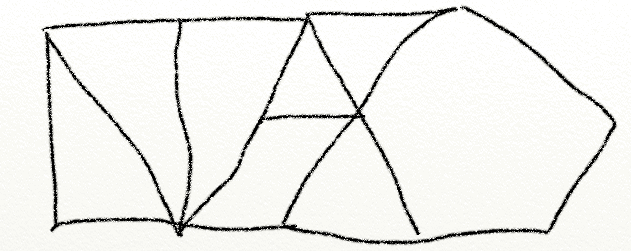
\includegraphics[width=\vismWdPercent{80}]{img/Nivazo-Hand-Drawn.png}\end{center}

            This symbol contains the letters for “NIVAZO” squished together and stylized into a sigil. On the rare occasions when someone asked me what it meant, I would reply, “Buddhist heaven is called nirvana. It is a place of bliss, peace, and connection. \emph{Nivazo} is my word for Buddhist hell, a place of chaos and total disconnection.” I had no idea that the real Buddhist term was \emph{samsara}. So, not knowing that, I apparently felt I needed to give my experience, which involved an acute sense of chaos and disconnection, a name, and so NIVAZO it was. From my current perspective, I consider that very unusual bit of precocious insight to be suggestive of some sort of Dark Night process. Anyway, it is interesting how, in retrospect, we try to make sense of our early lives, to fit the mysterious actions of a child into the simple boxes that an adult can understand.
        \chapter[Bodysurfing]{Bodysurfing}

            I have spent hundreds of hours bodysurfing at the beach between my childhood and adult life. I was bodysurfing this morning before I wrote this section. I started when I was probably ten years old, and spent many hours doing this every day when my family would go on beach vacations, which I have gone on at least once per year since then. Bodysurfing taught me a lot about waves. To catch a wave and have its power send you shooting out across the flat water in front of you for a long distance, you must time your jump into the wave exactly right. The wave itself must be just right, must be curling just right, and you must catch it at just the right time. The water the wave is breaking onto also must be just right: smooth, not too shallow, and at least stationary or, more optimally, pulling back out to sea, as that maximizes the speed difference between you and that underlying water, which helps you keep your head up so you can see where you are going, enjoy the speed, and steer properly.

            If your timing is not perfect or the wave is not just right, either you won’t get caught by the wave or, when the wave catches you, something bad will happen, like getting forcibly tumbled into the sand below the water. If you catch the wave just perfectly, and the water below you is perfect, you can go shooting towards the beach for a long run, head held up, with great control of your direction of travel. It is a thrilling feeling. I bodysurf with one hand out in front to steer and one hand below me to give lift to my head so that I can see where I am going, and I prefer that greatly to the style where you are head-down in the water. Head-up bodysurfing makes for much longer, faster, more enjoyable rides.

            To feel all the conditions simultaneously to catch just the perfect wave at just the right time with just the right underlying water requires modifying your brain and attention such that you become a wave-reading creature rather than one concerned with anything else, as you quickly learn the potentially painful consequences of getting it wrong. While some of this eventually becomes intuitive, it requires great immersion in the moment. Your feet and legs feel when the water just above the sand is pulling back towards the sea. Your torso and arms can feel the right moment to jump into the wave on the surface. Your eyes become attuned to the exact curl of the waves coming towards you and the depth of the water you might be hurtling over. You can see exactly the angle of the breaking wave and whether there are other waves that might interfere with that wave, either by coming into it sideways or running over it. Your ears hear waves behind you as you finish your run such that you can avoid being slammed down into the sand when you try to stand up. You also must watch for those around you such that you don’t crash into them. That is a lot to pay attention to—a rich and engaging world of forces, movements, tensions, fluxing, and flowing to get lost in.

            When you get it just right, feeling the perfect convergence of forces and fluxing, you are richly rewarded, as the power of the wave catches you, and you shoot towards the beach. That word “convergence” is important, as this style of bodysurfing requires everything to be just right for it to work properly. When you get it wrong, sometimes you just miss the wave, and sometimes the wave puts you through the spin cycle and possibly drives you to the bottom. The larger the waves, the greater the reward, but also the greater the punishment when you have improperly gauged all the factors, and the potential to get badly hurt or die is very real. I have bodysurfed on waves whose curl was up to about eight feet high above the surface of the underlying water, but wouldn’t recommend that until you know what you are doing, and perhaps not even then. Often your positioning isn’t quite right, or the wave isn’t quite right, or the other conditions aren’t quite right, and you must either dive under or jump over that wave, which is itself another skill in wave-reading and negotiation.

            I think that the many hours I have spent bodysurfing were invaluable for my vipassana practice as, once I got the hang of vipassana, I found that it was often just about feeling those same sorts of waves, convergences, and flows, but this time for objects like attention itself and the motion of energy in the body. Even space fluxes, and we can learn to ride those fluxes into perfectly converging moments of clarity just like we can learn to ride waves in the ocean. When everything converges just so, that can cause important shifts in our perspective that bring the various states of concentration and stages of insight. While I wouldn’t necessarily recommend bodysurfing, as it can be dangerous, I think that it honed underlying skill sets that translated well into meditation. If you decide to try this style of bodysurfing, please take responsibility for your own actions and safety, doing it with people around, on waves of reasonable size, on a soft, sandy beach without rocks or other hazards.
        \chapter[College and Pre-Buddhist Exploration]{College and Pre-Buddhist Exploration}

            The next time I remember crossing the A\&P was the summer after my junior year in college at UNC-Chapel Hill. I had been philosophizing heavily and hanging out extensively with my housemate Kenneth Folk. He had also crossed the A\&P a few times by that point, back in California, using totally different methods, and at the time he also didn’t know what it was. We lived together with my friend Chris in a grungy band house covered in acid-art from the previous tenants. Kenneth and I often philosophized furiously while playing Frisbee in empty parking lots late at night. We spent countless hours searching, reading, discussing, and debating things related to what we felt were the deep questions, particularly topics such as free will versus super-determinism, unitive models presented by physics, and the tensions with dualistic human experience. This is not something depressed people tend to do, more like something obsessed people do, and we were obsessed with trying to figure the thing out, though we weren’t even sure what “the thing” was.

            Our hunt was somewhat eclectic, including the poetry of T. S. Eliot, the writings of Tolstoy, and authors such as Ken Wilber. During that time, Kenneth and I forged a deep friendship. One of the key topics we had been discussing was the observer or watcher and how this related to the question of non-duality. Kenneth took off after that school year, going back to California to start the more formal, meditative phase of his spiritual quest, and I was still living in the grungy acid-art band house. I had no classes for the summer and was just working about two or three nights a week running sound for bands (which was my living all through college and for two years thereafter), so I had a lot of time to do basically nothing.

            One day, I was just sitting on the couch when I decided to take on the watcher directly. I am not sure exactly what inspired this practice, as Buddhism in a formal practice sense hadn’t shown up in my life yet, but trying to make sense of my experience just seemed to be the right thing to do at the time. I began trying to catch the watcher, second after second, really going after the visceral, perceptual experience of what was observing, and before I knew it, got into this rapid-fire back and forth, super-concentrated state of everything vibrating in my head, and the whole vibration zapped back through my skull at very high speed into a black space, and it was done. The whole process from start of contemplation to finish couldn’t have lasted but a minute or two, and the quick zap lasted less than a second. There were no other fireworks, no bright lights, no amazing dreams, no bliss, nothing. Just that, but that was all it took. I broke up with my girlfriend of the time for no particularly good reason, moved into an apartment alone, and was relatively dark for a while.

            Interestingly, that particular girlfriend would later become my first wife, and that means that she was already experiencing some of the unfortunate side effects of being in a relationship with a practitioner, except that I wasn’t a practitioner that I knew of, except that I unknowingly was. I mention her because she is quite important to the story, except that I am not going to say a lot about her. Despite her very social persona, she was a relatively private person in many ways, and I respect that privacy. Our stories are extremely connected. She was on retreat with me for most of the early retreats, and with me during my travels and travails for the first six years of my dharma practice.

            The take-home from it all is that early dharma practice and relationships can be a rocky road, particularly when both people are dealing with various stages of insight, though just one going through it can be more than enough to cause trouble. I owe her a lot, as she was very supportive through most of it, and I wish her all the best. While she was there for many formative parts of my journey, most of the story hangs together pretty well without going into details about her, and the dharma lessons are the same. I transmit many of the lessons I learned from my interactions with her and the dharma in various places in this book in generic ways, so hopefully the practical message gets through without having to go into specifics. My gratitude extends to her for everything she did to support my practice and teach me about life.

            The third time I crossed the A\&P occurred during the year after graduation from college. I was dancing in a club while running sound for a great dance band called Mr. Potato Head, and I began spinning around and got into a very altered state, dancing wildly, with tremendous energy, feeling an intense and cathartic long-sought freedom, like something I had forgotten, and an amazing bliss and sense of power welled up through my being, overtaking the dancing, and dancing me effortlessly but with this cone of raw power in the center around which the world and my body were spinning and moving quite on their own (Wiccans and whirling dervishes take note here); and then it peaked in joy and intensity and was done. After that I began to have to meditate to feel “normal”. I would go outside before work, lie on the ground, breathe very slowly, and somehow that would help a little. Shortly thereafter I got frustrated and angry at the band I was running sound for, quit working for them, got a job as a cook in a gourmet seafood restaurant called Squids, and then moved to California for a while.
        \chapter[The Middle Years]{The Middle Years}

            I don’t recall when I next crossed the A\&P, but I know the effect it had: I suddenly needed to go on retreats, so I did. I had done no formal meditation practice since fourth grade, knew little of Buddhism, but on the advice of Kenneth Folk, I went on a nine-day intensive insight meditation retreat at IMS with Christopher Titmuss, Sharda Rogell, and Jose Reisig in August 1994.

            Backing up just slightly, some explanation is required here. I went on that retreat not only because the A\&P was continuing to drive my desire to find spiritual answers, some resolution to the tension and questions that it created and half-answered, but also because long meditation retreats had visibly benefitted Kenneth, who by this point had done the three-month retreat at the Insight Meditation Society (IMS) and then, a few months later, went to spend six months on retreat at the Malaysian Buddhist Meditation Centre (MBMC) and then, immediately, six months more at Panditarama in Burma, for a total of a year-long retreat in Asia. We had been on the road together in a band and lived together for most of a year. Those sorts of close experiences show the various sides of everyone involved. It was quite apparent that his meditation practice had done something very good for him, though exactly what that was I couldn’t put my finger on, as this was before the phase in which Kenneth and I got into talking much about the details of practice and results. So, I went on that first retreat.

            As a hopefully instructive and normalizing aside, when I started my first retreat that summer in 1994 at IMS, I quickly realized that I could barely feel my feet. It was not that they were numb, or that I couldn’t really feel my feet, but my attempts to follow the basic walking meditation instructions, “Notice the sensations of the feet touching the ground, of the feet lifting off the ground, of the feet moving through the air, the feet touching the ground again,” were nearly completely thwarted by a mind that seemed to have almost no ability to do something that would have seemed trivial had I not done the experiment and found otherwise. My ability to stabilize attention on my feet was nearly nonexistent, the sensations were vague, fragmented, confusing, and the wash of frustration, wandering thoughts, and other distracting sensations that poured in nearly eclipsed whatever data was coming in from focusing on my chosen meditation object.

            Thus it went, walking period after walking period, day after day, and finally after about five days I resorted to drastic measures and started walking barefoot on the tops of the classic New England rough stone wall that lined the road. Now, I should say here that I am not sure this would be a great solution for everyone, or even for most people, or necessarily anyone other than me in that specific place and time. There might have been a better solution that I just didn’t think of or know about. I am not advocating inflicting pain on yourself so that you learn to practice well, though in truth I have done this many times; done in the right circumstances after making sure it won’t cause permanent damage, it can, at times, produce some benefits.

            I must be careful here, given that the audience of this book might contain some pretty gung-ho practitioners, and it would be very easy to take this too far, which I definitely don’t advocate. That said, it worked well, as suddenly the pain rose above the din and chaos of a totally untrained, distracted, ordinary mind, and there was finally some real clarity. Now, it could be argued that there was some clarity that recognized the din of a totally untrained, distracted, ordinary mind, and we could debate the merits of that point of view, but, for practical purposes, the din had been going on for years and gotten me no place good.

            There were feet, there were stones, there was pain, and lots of it. I am not into pain, just in case anyone thinks I am sounding masochistic, or that I am fetishizing pain in any way. However, it was a very strange relief to suddenly be able to notice a universe of sensations where before there had been only extremely frustrating vagueness. Every little prick, sting, burn, and scratch was experienced suddenly with a level of detail and precision that had until then been lacking and, while quite unpleasant, it felt like I was finally beginning to get what was going on, what I was there to perceive.

            When I have told people this story, many have responded with statements like, “You’ve gotta write that down, as people probably think that because now you can do all sorts of cool stuff with your mind that from the beginning you were just a natural or aberration or something”; in fact, this is not true at all. I started out with the same messy, disorganized, attentionally flabby mind that most everyone going on retreats begins with. I was also very committed to changing that. When I started practicing and realized that even the most basic and seemingly simple instructions were entirely beyond my capabilities, that really rankled my pride. It grated against my dearly held vision of myself: that I \emph{should} be able to follow more than three breaths in a row without being invaded by my neurotic stuff, to say nothing of being able to feel my two feet upon the ground.

            Many people consider pride and having a vision of ourselves being a specific way as antithetical to spiritual ideals such as humility and dissolving any sense of a self at all. It is not that humility isn’t a very good thing. Dissolving any sense of an observer, controller, or doer is a very good idea and basically most of the point of all of this. However, in relative terms, having a vision of yourself in which you aspire to have a well-trained mind, well-developed attentional control, and strong sensate clarity are of such inherent and fundamental value, in my view, that any positive hook that gets you some strong fingerhold in that territory (or even a good glimpse that you can remember) to keep yourself motivated to practice enthusiastically and well makes that hook skillful.

            It is very important to identify your own personal skillful motivators and work with them, allocating their energy for practice. What drives you? Why are you into these things? Most of us are into strong practice for a mix of reasons, most of which are common, but each of us has our own personal story, our vision of ourselves, the demons we are wrestling with, our dreams and goals that get us out of bed in the morning, our own great archetypes of mastery that call to our deepest longings and aspirations. If we know what those are and can draw on them to keep going and keep on pushing ourselves to continue to transform our hearts and minds in truly amazing ways, we will likely do much better.

            What are the recognized hooks that compel people to practice well? I have already mentioned one of them—pride. I do not mean the afflicted variety that is synonymous with conceit, but that positive quality by which we have set a high standard for ourselves of what we are capable of accomplishing and perceiving. I value the ideal of having a mind that is clear, bright, easily directed, nimble, quick, steady, broad, deep, inclusive, powerful, and that directly perceives the truths of experience as its baseline. I value the ideal that we can be kind, compassionate, mature, poised, equanimous, and doing good in the world. I value the ideal that we can be a people with a vast range of capabilities, with profound and nuanced understandings, and a great ability to help others, as well as the openness and realism to accept the cold, hard facts of being born a mortal mammal. Call it skillful vanity, enlightened self-interest, confidence, divine pride, or whatever mixed term acknowledges the pitfalls of this point of view while recognizing its great potential to inspire skillful striving that can transform our own and others’ lives in very positive ways.

            Pride, as distinct from its shadow aspect of arrogance or conceit, was one of my primary motivators and a strong one. Many have pointed out that they detect—in addition to the pride I have taken in practicing well and sharing the fruits of these explorations with others—an arrogance verging on hubris in this work. Their point is clearly valid. That said, arrogance is something that I am called upon to work with daily in my job as an emergency medicine physician, and all I can say is that this profession has served as an antidote to arrogance, as the facts of mortality and the suffering inherent in the human condition are uniquely humbling, but which thankfully do not dampen my enthusiasm for either meditation or medicine.

            About six days into that first retreat, after various episodes of back, neck, and jaw pain, as well as the discomfort in my feet from walking on stone walls, I was just sitting there, and suddenly I noticed that my body was not solid, but instead made of zillions of tiny particles of energy, all moving around, zipping in and out of reality, and my body exploded, everything flashed black and white, and I felt as if I had been dropped back onto my cushion from space.

            After that I was hyper-energetic, hyper-philosophical, and yet convinced that philosophy as I knew it held no further answers, but I had no idea what to do next. No one told me what had happened or what the stages that follow the A\&P could do to you, and shortly thereafter I quit my electrical engineering undergraduate program and went to India for about a year to meditate and do some volunteer service.

            I had been getting straight As in that electrical engineering program and loved it. I also hoped it would get me a better job than my English BA had gotten me. Further, when I got to differential equations, I felt like I was staring in wonder at the language of God. Differential equations describe lots of systems uncannily well, but they are particularly apt at describing systems involving the oscillation of potential and manifest energy, as well as any other vibrating system. To me, it was like the deepest philosophy, the key to the essence of what was really going on. That differential equations do their magic using a number that doesn’t exist, the square root of negative one, interestingly called “i”, was unusually profound to me at the time. I attribute that profound appreciation and remarkable ease of understanding of the deeper meaning and uses of differential equations to having crossed the A\&P.
        \chapter[Thank U, India]{Thank U, India}

            My first wife and I ended up in India due to many complex factors, but some major ones stand out. First, as mentioned, I had crossed the Arising and Passing Away again on my August 1994, nine-day retreat at IMS, and somehow it strongly sparked my interest in doing something more directly helpful to people than the electrical engineering program was likely to lead to, so I began seriously thinking about medical school again for the first time since I took my MCATs after my sophomore year in college. Second, on the last day of the retreat at IMS, Christopher mentioned that we were all welcome to join him for his yearly ten-plus-ten-plus-seven-day retreat in Bodh Gaya, India, that coming January.

            Then, I met with a member of the UNC-Chapel Hill Medical School Admissions Committee, who looked at my rambling path and said, “You know what would really pull this application together? Go immunize Tibetan yak farmers, relocate Rwandan refugees, or something like that.” So I began writing letters. It turns out that finding volunteer positions overseas is not something I am very good at. I wrote many letters to many organizations offering to help, and the only response I got back from all those letters was a single small, hand-written note from a nun at Mother Teresa’s Missionaries of Charity (that I still have) which said simply that they couldn’t give me anything—food, lodging, or money—but that if I wanted to come help, there was a need. Based on that small piece of paper and the promise of a longer meditation retreat where the Buddha himself got enlightened, off to India we went.

            My year in India changed me more than most other years of my adult life. In retrospect, I am extremely grateful for that year, but at the time I was so in it that I didn’t appreciate it as much as I do now. Though service work was not new to me in the context of church, Boy Scouts, hospital volunteering, and so on, going from Raleigh, North Carolina to New Delhi, India—whose beggars and commission agents hit you like a screaming wall of technicolor insanity when you walk out the door of the airport—was a total sensory assault. Things only grew more so as the year went on.

            What I found most striking about India is that everything is right out in the street in its full range of wonderful to horrible in a way that is very different from the United States. Birth, sickness, old age, and death are all right there. I watched bodies burn on the river Ganges in Varanasi. I saw drugged babies rented to beggars to increase their daily take. I was robbed, molested, harassed, and generally taught remarkable lessons in impermanence, boundaries, and the human condition by the good citizens of India as they understandably tried to survive and be okay in that chaotic yet wondrous place.

            If you have grown up in a place like India, this doesn’t surprise you. But, coming as I was from suburban USA, it was beyond eye-opening and into the realm of brain restructuring. Similarly, when I came back from India, it was like the symphony suddenly stopped, the doors closed, and everyone was in a building or a car, and most of what I saw when traveling around were just structures and machines rather than fragile, resilient humanity in all its glory and misery. This was similarly shocking, as I had gotten used to seeing everywhere what life’s rich pageant had to show.

            Beyond just seeing it, I found that India is interactive in a way that the United States is not. People everywhere wanted to talk, to sell things, to ask for gifts, to take me to their shop, hotel, or home, to steal what I had, and to teach me things. Many of them, had you asked them, would never have said they wanted to teach me things, but that was what I finally realized they were doing, though I often didn’t appreciate this at the time.

            It is no accident that the first noble truth taught by the Buddha is: there is dukkha, and that this teaching was first given in India, where suffering, just one aspect of the word “dukkha”, is everywhere and glaringly obvious. I should add that I spent most of my time trying to help people in some of the poorest parts of Calcutta and in some extremely poor villages outside Bodh Gaya, which are some of the poorest and most corrupt parts of India, so my perception is a bit skewed. What sick and twisted trick of my Dark Night had dragged me to these places at the bottom of the barrel of the human condition I have no idea, but I now feel that something odd was doing its spiritual work, though I didn’t think of it that way at the time.

            The deformed beggars, the starving children, the flies and mosquitos, the coal smoke–filled air, the heroin addicts, the lepers, the people with visibly horrible diseases, and the staggering corruption: all that I got to know almost immediately, but it was mostly visual, auditory, and olfactory, even though it also had a deep emotional impact. However, when I began to get some of those diseases myself, lose weight, and become an intimate part of the dance as India began to do its remarkable work on me, that was when some of the deeper truths of dukkha really hit me, rather than just on the cushion investigating the three characteristics.

            I got giardia and amoebiasis, as well as various other forms of bacterial dysentery, more times than I can count, but at least twenty. I lived on something called Tiz DF (tinidazole plus diloxanide furoate) and sometimes ciprofloxacin. When I got hookworms, I took a veterinary de-wormer called Kit-Kat, not to be confused with the Nestlé candy bar. We got dengue, which we actually got in Cambodia in an attempt to do service there that didn’t work out. It hit us on the plane to Bangkok on our way back to India, and I simply lay nearly prostrate for a week with fevers to 104°F in a cheap, un-air-conditioned hotel in Bangkok, feeling like I was going to die or tear off my aching head. I was so weak I was barely able to stand for about five days, crawling slowly down the stairs to get a bit of Pad Thai and drink some water before slowly crawling up the stairs back to my room to lay semi-delirious and pouring sweat in the un-air-conditioned summer heat of Bangkok, wishing my splitting headache would finally end.

            I got hepatitis (likely E, as I was vaccinated against A and B, and later tested negative for C) while in Bodh Gaya, and got my second case of hookworms while I had that, but, given that I had no idea what Kit-Kat would do to my liver, I left them untreated, tolerating their total creepiness until finally I wasn’t yellow and I could walk without terrible pain in my bloated liver. I also passed a five-millimeter kidney stone while I had the hepatitis and the hookworms, and at that point, now about 135 pounds at six feet tall, dark yellow, all I could think while I lay there in broken misery was, “If one of those mosquitos humming around the outside of my mosquito net gives me malaria, I am truly a dead man.”

            After about eight months of almost continuous, mostly gastrointestinal illnesses, strangely my body suddenly seemed to come to terms with the Indian flora and the illnesses stopped. My weight didn’t come back until I finally got home, but at least there seemed to have been some sort of truce. I was still drinking the local water, still eating the cheapest street food, still crossing large rivers full of sewage barefoot to get to the villages that I was trying to help, still getting bitten by a lot of mosquitos, but somehow it was like my immune system had figured out what it needed to do and I was finally sort of okay. But by that time, I was moderately traumatized and Dark Nighting so hard that I hardly seemed to notice or care, as the illnesses just seemed to be one more element of a great wave of total misery that was breaking me down.

            Backtracking to the early part of my time in India, when I made it to Calcutta after a month in India and started to work at Kalighat, Mother Teresa’s Home for the Dying Destitute, I think I was in shock, but not the sort of shock that was immediately obvious. I don’t think that people looking at me could tell I was in shock, nor did I myself recognize that I was in shock at the time—that dawning realization about what my experiences in India had done to me would surface much later.

            At the time I was energetic, engaged, interested in trying to make a difference, getting up early, walking to Kalighat, the Kali temple for which Calcutta is named, with its women lined up and down the street with goats for sacrifice, going in to the Home for the Dying Destitute, helping the men who lay there. They had tuberculosis, cancer, large sores, missing limbs, blind eyes, and other serious health problems. One of them strangely was a Danish tourist who had gotten hooked on cheap heroin, spent all his money on it, ended up homeless living on the streets where he shot up with dirty needles, and finally got such large, infected sores in his arms that significant portions of flesh were simply gone and you could see large swaths of arm bones through the gaping holes. He was an oddly smart, educated, articulate, and personable fellow, dying there in that home of charity in India. Like I did with the others, I helped him change his bandages and take his medications, brought him food, helped to keep him clean, as his arms barely worked anymore, and did my best to try to ease his suffering in what limited ways I could.

            I think that the initial shock partly insulated me from what was going on in the radically altered circumstances I now found myself in, allowing me a moderate degree of functionality. We were living on cheap street food, eating in the cheapest restaurants, cooking what cheap food we could buy in the local markets and cook on a little kerosene stove on the roof of Hotel Modern Lodge, an un-air-conditioned but relatively secure hotel in the skanky end of the tourist district in Calcutta. We did our laundry in a bucket, showered with cold water (which was okay, as it was already hot by February, and just got hotter as the months went on), and purified our water with a hand-pumped camping filter and betadine (which would eventually trash my thyroid gland). When the monsoon came, the streets flooded two to three feet deep in sewage for a few blocks, and we had to walk carefully to avoid falling into the manholes that were opened in such circumstances to help the streets drain. I give thanks to the other volunteers we met there for their camaraderie, support, and exemplary dedication to helping people.

            After a few weeks at Mother Teresa’s, I switched to a street clinic called Calcutta Rescue about forty-five minutes north of the hotel by bus, where I mostly worked in the pharmacy and the vitamin A project, but did a few other office and logistical tasks as well. The clinic saw about 200–500 patients per day and more patients down the road by the river at an affiliated clinic for those with leprosy. We got there early, stayed late until everyone had been seen, then would take the buses home through the maddening Indian traffic to the hotel, cook food, try to sleep in the sweltering heat, get up, and do it again. The patients were generally extremely poor, many with tuberculosis, many with other serious health issues already mentioned, many with parasites, some starving, and we would try to give them what food and medications—as well as wound care and other helpful things we could—depending on what we had available at the time.

            I remember a mother who had a few children with her, one of whom was a little girl who appeared extremely tired, sick, and emaciated. The child was probably two years old, but functionally she seemed like a very sick one-year-old. Through a translator, I asked the mother what was wrong with the girl. With apparent calm dispassion that likely masked terrific agony, the mother explained that she was starving her daughter to death, something the mother had done with previous daughters, as she was very poor, had no money for the girl’s dowry, and needed to be able to feed her sons. That is one of many similar encounters I would have at that clinic, if that gives you a sense of the place. While there was something about the fact that we were all there to help that did make the misery more bearable, still, those sorts of situations can strike very deeply, sometimes deeper than we may realize at the time.

            I remember the heroin addicts who lived in the alley just outside the hotel door. There were typically five or ten of them—long-haired, naked, skinny as rails, covered in dirt and ash, and covered in sores from infections by dirty needles. I recall some lying there high as kites, others clearly in withdrawal, shaking and vomiting, others shooting each other up with little brownish vials of cheap heroin. What I noticed is that nearly everyone else in India seemed to want to interact with tourists except the heroin addicts. They didn’t look at us, didn’t seem to see us at all, didn’t ever say anything to us, as though they were existing in some parallel ghost realm that was only loosely connected to this one. I can’t help but think of them two decades later whenever I hear the phrase “hungry ghost realm”.

            I remember coming home from the street clinic one day and there was one of them lying on the ground with his arm deep into the open sewer that ran along the alley, slowly crawling along, arm about two feet into the sewage, apparently looking for something. I was curious and, as the heroin addicts never interacted with us at all, I stopped to watch what he was doing. He ignored me and my curiosity entirely.

            For about five minutes he felt along the bottom of the sewer, carefully, patiently, inching his naked body along the ground, and finally he stopped, a small smile crossed his face, and he pulled out a syringe from the bottom of that Calcutta sewage. He licked the bare needle, broke off the top of a small vial he had concealed in his other hand, drew up, shot up right there, and lay back in a daze on the street, dirty needle still hanging from his arm. It struck me that, when you are shooting up with a needle from the bottom of a Calcutta sewer, you have likely fallen much lower than you ever thought you could fall. I wondered at that point who he had been before, what his parents felt about him, what any children he had might have felt about him, and how much longer he could possibly live.

            That snapshot of his suffering would be driven even more deeply home some months later. I was again coming home from the clinic and saw the same man, sitting on the street cross-legged and crying, tears streaming down his face. In his hand was a single white index card that was perfectly clean. He had managed to gather seven extremely small pieces of colored chalk in a little pile on the ground to his side, and had drawn a rainbow on the index card. He was staring at the rainbow and crying his eyes out.

            I realized there was likely nothing at all I could do for this man, but something in his weeping humanized him for me such that months of being in shock could no longer be kept at bay. It felt like that man had torn my heart out, as if suddenly the pain I had somehow managed to numb partially, so that I could do the work and live as I was living, came crashing in with the full force of a tsunami. The hairs on my arms still rise now over twenty years later when I think of him. I am deeply grateful to that naked, dying, addicted artist, though I would greatly prefer that he hadn’t been dying in misery on the streets of Calcutta, and that I hadn’t needed something like that to shock me into realizing what was going on.

            It is said that the Buddha left his pleasure- and distraction-filled life in the palace for the first time at age twenty-nine with his charioteer Channa, saw four people—an aging man, a sick man, a dead man, and an ascetic trying to find the end of suffering—and rapidly came to deep conclusions about the nature of suffering right then. I was obviously dense as a post in comparison. I had also come from a sheltered palace, suburban North Carolina, and it took some six months in India, seeing tens of thousands of people suffering in horrendous ways, until finally something in that moment with the weeping addict slapped me into reluctant appreciation for the depths and realities of human suffering. Shortly thereafter I felt a deep need to go on retreat, so off to Malaysia we went.

            While this may sound like a horribly clichéd thing to say, I am truly, consciously, and actively grateful every single day that I am lucky enough to live in a remarkable place, have good food to eat, have good medications, and amazing resources to help patients. I am very grateful that I have my health and that I didn’t end up dying some horrible death in India. Lack of gratitude is endemic where I live, which is ironic, as it is the richest country on Earth.

            It is also worth mentioning that I didn’t go to India with the intention of purifying my karma or anything like that. I went to help people, for meditation, for adventure, to try to resolve my spiritual crisis, and to learn something about myself and the world, but I don’t remember ever thinking while I was there, “Wow, I hope all this hard work, suffering, and accumulated good karma from serving the destitute gets me a good rebirth or gets me to stream entry fast!”

            In retrospect, I do believe—in some way that a strict scientific materialist might think was some mix of crazy and/or irrational—that somehow doing all that work there did help to purify something karmic and help my meditation practice probably much more than I will ever know. That was never my goal, intent, or even thought at the time, as I just didn’t know any better.

            Beyond the karmic opportunities, which you will find anywhere there are people, India had many other remarkable qualities. Out of that muck and insanity come extraordinary things. It is not just ancient India, the India that brought us the Vedas, the Upanishads, and the Buddhadharma, but also modern India. There are deep aspects of spirituality and beauty to be found there. I met true living saints there who were humbly and inconspicuously serving some of the most impoverished people in the world. I met numerous people with deep spiritual realizations, many of whom were seemingly ordinary folk doing very ordinary things. I met people who were amazingly happy, bright, and cheerful despite circumstances that would bring many to unmitigated despair.

            I remember the many street children I got to interact with, and the children out in the very poor villages where we tried to help. Those with the physical and mental ability to do so played, laughed, joked, danced, skipped, and seemed to enjoy themselves despite being among the most underprivileged people in the world and dealing with circumstances that modern civilization, if it actually is that, should have eliminated long ago. I often find myself thinking back to those kids and the profound lessons their sunny attitudes and just being themselves taught me, and that however bad I may think I have it, it could be a hell of a lot worse. For most people and creatures on this planet, it is. That recognition naturally prompts gratitude, and that helps immensely when I am faced with the comparatively milder challenges of my daily life. As the Alanis Morissette song says so well, “Thank U, India!”

            Another practical point here is that, should you find yourself in your meditation practice or just your life feeling sorry for yourself or becoming overwhelmed by your issues and life, particularly if your circumstances are, in relative terms and compared to the rest of the world, good to great, then think about stepping outside your comfort zone and going to try to help someone less fortunate than yourself. The very least you will learn is that you could have it much worse. Far beyond that, you will likely make friends, help people, and spread the spirit of doing good in the world, and you will likely be cured of self-pity forever or for a long time.

            Even beyond that, as you probably already know, you will likely learn very important lessons from the people you find in the ditches, deserts, and dungeons of this world, as many who live there have had to learn profound spiritual lessons to survive, lessons you might not yet know, or at least such has been my experience. Thus, should you go to help people, expect them to be the ones helping, growing, and blessing you, though not in the ways you likely expected. Just as many of the best addiction counselors are themselves recovering addicts, and many of the best psychiatrists have their own experiences with crazy, just so, many people who are living at the proverbial bottom of the barrel of the world have had to grow spiritually in surprising ways to cope with that.

            Further, many of the other people you find alongside you helping to ease the world’s suffering may be living saints in disguise, and there is much to be said for hanging out with living saints. Getting out of our palaces and bubble bath zones, assuming we are lucky or unlucky enough to be living in them, and getting our hands dirty helps broaden our horizons, expand our awareness, and make this a process about something much bigger than ourselves. Even if you are just a complete spiritual materialist or narcissist concerned only with your own spiritual growth, development, and attainments, there is much there for you in the world of serving others, which, word has it, is the point of all these traditions. Paraphrasing the Fourteenth Dalai Lama: If you are going to be selfish, be wisely selfish, and do what is truly in your own best interest, which in this case means trying to help others.

            In that same vein, as it were, I believe that the experiences I had while trying to help people but often failing to make what seemed like any significant difference, getting sick, and realizing that I had it pretty darn good helped me to get over myself just a teensy bit. Thus, when I was finally able to go back on retreat in Bodh Gaya, retreat seemed like such a refuge, such a blessing, so precious, so clean, so sane, so safe, so stable, so beautiful, so quiet, and such a fortunate set of circumstances that I could make much better use of that time because the contrast with Calcutta and the outside world helped me to truly cherish the incredible opportunity I had.

            Death by disease, auto accident, or other bizarre circumstances no longer seemed to be just moments away, as it had so often seemed on the outside. Here, on the retreats, were order, true “civilization”, clarity, peace, and an opportunity finally to go deep to see how to deal personally and directly with suffering, undistracted by the colorful madhouse that was the streets of India. I could let my guard down and plunge deep into the waters of techniques and teachings that also originated in the wonderful, profound aspects of India. Thus, what might conventionally be thought of as the good and the bad of India were both of supreme value, finally, and that is one of the lessons that slowly sank in during that year or so, and in the years that followed.
        \chapter[The First Bodh Gaya Retreat]{The First Bodh Gaya Retreat}

            Speaking of retreats, and backtracking just slightly to the beginning of my time in India before I went to Calcutta, the next time I crossed the A\&P was about five months after the August 1994 retreat. I was then twenty-five years old. I was on my second insight meditation retreat, this time during a seventeen-day course at the Thai Monastery in Bodh Gaya, India, with Christopher Titmuss, Sharda Rogell, Subhana Barzaghi, Norman Feldman, and Fred von Allmen. I don’t really remember much about it, except that it left me feeling very inspired about practice and very dark about the “world”. However, three formative events stuck out.

            The first was when Subhana Barzaghi, one of the meditation teachers on that retreat and a dual-lineaged Zen master and vipassana teacher (a very rare accomplishment indeed), answered a question from a retreatant during a small-group session. In that answer, she described how she would meditate on the breath for an hour or so and then attain a Fruition. She described it as if she was describing any other ordinary activity. There was nothing cryptic about it, nothing mysterious, nothing guru shi-shi, nothing pretentious, nothing self-effacing, nothing taboo. It was just straight-up reporting of her experience, her capabilities, her practice—articulated like it was the most natural thing in the world, like she was talking about what she had for lunch. It was the first time that I had ever heard that done in a way that was so down-to-earth and real, so straightforward, and, by example, so empowering. That experience would form the basis of the model I would later adopt, advocate for, attempt to emulate, and encourage. I offer Subhana very special thanks for showing me that it is possible to discuss deep practice as we would discuss any other ordinary activity.

            Second, I remember Norman Feldman’s late-night readings, particularly his reading of the Pali sutta that would later become one of my favorites, \emph{Majjhima Nikaya}, 121, called “The Shorter Discourse on Voidness”. I found its words spellbinding, and the thought arose, “Ah, this is it! This is the real thing!” To this day, I still think that. I am very grateful for him sharing that text with us by candlelight late that memorable chilly night.

            Third was Christopher Titmuss himself, for whom I have profound gratitude.\footnote{\vismAssertFootnoteCounter{X}Yes, I am aware of the controversy regarding Christopher Titmuss.} His embodiment of awakening as a living truth was palpable, open, and inspiring. His cultivation of awakened teachers around him who were from not only various strains of Buddhism, but also from traditions outside Buddhism, embodied a spirit of pragmatism and non-dogmatism regarding awakening as a human right rather than the property of some religion—that was a rare example of what is possible in terms of dharma cooperation. His message of engagement with life in all its rich and complex tragicomic glory, delivered from a place of awakening and encompassing a full range of powerfully articulated emotional reactions to a wide range of real-world topics, modeled lessons that it would take me years to assimilate.

            Inspired by that retreat, I tried to sit for an hour every day and managed to do that most of the time. Those sits resulted in no particularly interesting insights or anything else that stands out, but I do suspect that just trying to keep up some basic skills helped. As noted above, after a few weeks volunteering at Mother Teresa’s original Home for the Dying Destitute at Kalighat, I began to volunteer full-time in a large, outdoor street clinic in the northern slums of Calcutta, called Calcutta Rescue, where I would serve for the next five months, mostly in the pharmacy and the Vitamin A project.
        \chapter[The First MBMC Retreat]{The First MBMC Retreat}

            Finally, the internal pressure took over, and I had to go on retreat again, so I went to Malaysia and sat at the \href{http://www.mbmcmalaysia.org}{Malaysian Buddhist Meditation Centre} with Sayadaw U Rajinda for two weeks, and that is when, from my point of view, I really learned to practice. It was about a decade after the first time I had crossed the A\&P, and I was about to learn what the Arising and Passing Away actually was, which seems a bit late, but that’s the ignorant, meditationally primitive Western world we live in.

            This was the first time I was introduced to noting and the maps, as it was my first Mahasi-style course. I had done more freestyle, Thai-style vipassana with Christopher Titmuss and crew and this had built some meditation skills, but I didn’t learn noting until this retreat. Initially, I was bad at noting, wanting to intellectualize everything, trying to note a decent amount, but not enough to get into any interesting territory or notice much about what was going on. About five days into the course, if I remember correctly, I was sitting outside the Sayadaw’s room and could hear a young Malaysian woman giving a simple, clear report of her ability to see thought as thought, intentions as intentions, mental images as mental images, and to see the physical sensations that were interspersed with these and how each led to the other.

            I came into the room, all jacked up on my intellect and basically talking out of my head about some philosophical bullshit that I can’t now remember specifically, and the Sayadaw just smiled and said, “That woman—did you hear her? She sees Cause and Effect!” The message was very clear in that instant: “Shut up, quit thinking, and practice!” or at least that was what I took him to be saying. It was very humbling, as I was basically an arrogant brat (still am, some would argue), but I had been totally schooled by this retreatant who hadn’t even been there quite as long as I had. I decided to really buckle down and note like crazy, and that is when the interesting stuff started to happen. Was this the competitive urge being used skillfully? Was I just too cocky to be outdone? Did I just suddenly learn something valuable from that practitioner and apply it? Was it all of those? Probably. Regardless, it worked.

            About two days later, my breath began to move with the noting. I would note “rising” or “falling” and the breath would rise or fall in nearly perfect synchrony with the duration of the note and then stop; so each stuttering breath became like rapid sniffing and took many notes, otherwise the breath would just stop. This was Cause and Effect (though I didn’t know it at the time). The same thing happened when I walked—the feet would move exactly with the notes, with rapid movement of the feet causing rapid noting, and rapid noting causing rapid, jerky movements of the feet.

            During sitting sessions things started to get wild, all just from noting everything that was going on. The rapidity of everything in the body jerking in conjunction with the noting got faster and more powerful, so that I shook, sniffed, sweated, and noted for days, and between bouts I would plunge down with the breath as it went down and down and down into a realm of extremely slowed perception and time, like reality was moving through thick, narcotic syrup, and then the energy would come back, and the rapid noting, sniffing, and the now powerful vibratory energy would return. It would cycle like this again and again. The whole thing was freaking me out a bit, so I went to Sayadaw U Rajinda and told him what was going on, and that I was concerned, and he simply said, “Not dangerous. Keep noting,” and smiled.

            I was sitting for two to three hours at a time with ramrod straight posture, which was very unlike me then and generally still is, was barely sleeping two hours a night, and sitting in a small, relatively private, air-conditioned room off to the side of the second-floor walking hall, as otherwise the sweating would totally drench my clothes. I was afraid that my violent periods of shaking and rapid-fire sniffing would scare people. After about three days of this, the whole thing finally died down. There was no specific event that stood out at that time as a specific A\&P Event, no blow-up of consciousness, nothing interesting in dreams, no big zap-through, and no bright lights or visuals at all. When it finally wound down after a few days, I was hungry for sex and chocolate, felt exhausted and sluggish, and within a day I could barely sit for five minutes, and my mind felt like a hive of angry bees. I saw a brief but very clear vision of a field of diagonally-arranged emerald skulls on a pale green background.

            That night, and at the peak of my frustration, Sayadaw U Rajinda played an old, scratchy tape of a Burmese monk describing the stages of insight, and suddenly everything was clear, or at least a lot clearer. I learned from that tape what had happened, knew where I was, and knew what to do about it. That tape changed my life, my practice, and my conception of practice. Lightbulb after lightbulb of understanding flashed on in my head, as that tape described in detail the experiences I had gone through, and it was just too freakishly accurate. That recording of a monk calmly reciting details, in order, of experiences that I had been sure were just weird, possibly unique, irrelevant quirks of my own strange practice, revealed that they were entirely stock, standard, and expected results of simply noting or even of just paying careful attention. That tape blew my mind. Sayadaw U Rajinda’s playing it at that moment was about the most kind, timely, and empowering blessing anyone could have done for me practice-wise.

            With a very high level of faith in the technique and despite the extremely irritating restlessness and powerful visceral aversion to practice that arose the moment I sat down, I resolved to sit on the cushion until I had passed Re-observation. It was horrible. It was like my mind and body were cracking open while being crushed and warped in sickening ways. I noted like crazy anyway. If you attempt to model your practice after this story, consider that this might not be an optimal strategy for you, and reread the section on Re-observation, which discusses various other options.

            Luckily, even though it was horrible, it did work for me. Within five minutes the horror broke, everything opened, the weight lifted, and very shortly thereafter everything got profound, abstract, and weird but in a totally cool way. So, whereas before there had been a body and a meditator and the usual stuff, now everything changed dramatically, or so it seemed to me, as I was meditating. Suddenly “meditator” was nearly gone except for a very vague background process. Body was entirely gone, the sounds in the room were gone, and what was left seemed to be two basic swirling, shifting, fluxing elements that I will approximate by calling very dark grey and blackest black that I would later describe as “suchness” and “awareness”, though at that point to say there was “color” is really pushing it.

            Suchness was basically almost completely formless, except that it seemed to swirl and synchronize with what seemed to be awareness, except that, wait a second, awareness was also just some other swirling, ultra-abstract, extremely hard-to-comprehend thing that was trying to sync with suchness. So, there was this shifting, swirling, nearly incomprehensible, totally stripped-down dark fluxing space dance that was going on; and there was the tension between the seemingly two things that, the more the practice went on, seemed to be \emph{nearly} just one thing, and it is that \emph{nearly} part that is crucial.

            I couldn’t land it. They didn’t synchronize on that last sit. I knew for certain that if those two things either became the same thing or synchronized and collapsed into each other, then that would be stream entry. I had no idea how long that might take. It turns out I was right, but I couldn’t make it happen at that time, as I couldn’t just forget about it and let it happen. It was too new, too fascinating, and too exciting,\footnote{\vismAssertFootnoteCounter{X}A stage I would later label something like ñ11.j7.j2, namely the second subsubjhana (exciting, amazing, too new) part of the Nothingness subjhana part of the eleventh ñana, in case anyone is asking.} which is the lesson that it takes some people a bit to learn. I had only an hour during that sit, which wasn’t enough time for me to learn how to just let it happen. The next thing I had to do was to leave and get on the Butterworth Express (great train, by the way) back to Bangkok. Coincidentally, Sayadaw U Rajinda had to go back to Singapore that same afternoon. I left MBMC. My concentration plummeted. My next attempt at sitting the following day was as ordinary as any of my previous daily-life sits, and then the hard stuff began.

            Such a precipitous drop in concentration and insight ability when leaving retreat is common. For most people it takes dedicated, repeated, daily-life practice of various skills to facilitate accessing those abilities when the daily dose of practice drops that far down again. There are some exceptions to this post-stream entry, but the basic point remains.

            I did have the luck to stop by the MBMC bookstore before I got on that train, and I picked up a copy of \emph{Practical Insight Meditation}, by Mahasi Sayadaw, \emph{Agga Maha Pandita} (which means arahant, incidentally), as well as \emph{In This Very Life}, by Sayadaw U Pandita (another arahant, but one whose book doesn’t have that title on the cover). I found \emph{Practical Insight Meditation} to be everything I was looking for. Here were the method and the maps. It was outrageously simple and straightforward, like the best practical how-to high school electronics or chemistry texts from the 1950s (geek, anyone?). I read it again and again, basically memorizing most of it. I give great thanks to that mighty monk in dark hipster glasses, as that book and the noting technique in it became my gateway to many amazing insights.

            Mahasi Sayadaw’s approach, and the resulting book \href{http://www.aimwell.org/Practical%20Insight%20Meditation.pdf}{\emph{Practical Insight Meditation}}, published in English in 1971, represented a massive foundational shift in the world of meditation. Its plain language, simplicity without sacrificing technical sophistication, directness, and emphasis on lived (not theoretical) phenomenology, along with clear, reproducible landmarks in practice, were paradigmatically groundbreaking. Unlike many previous authors who simply didn’t seem to trust their eyes and ears or their own practices as much as they deferred to the ancient texts for orthodoxy, Mahasi Sayadaw broke many taboos and dharma literature protocols and precedents when he wrote down simple, original, accurate, and helpful criteria for discerning various stages along the path based on clear observations of what happened when thousands of people practiced his technique at high doses. It is hard to explain to an audience who is now likely used to that sort of openness and phenomenology how this simple book and the paradigms in it raised the level of practical dharma discourse across cultures. My own practice and the world of meditation in general owe so much to that remarkable, revolutionary, yet—perhaps significantly—extremely traditional Buddhist monk.

            Speaking of traditionalists, Mahasi Sayadaw’s works received some serious blowback from some members of the establishment when they first appeared. Some of this persists today. However, for those who love the suttas and the Buddha’s core instructions, pick up \href{http://www.aimwell.org/Practical%20Insight%20Meditation.pdf}{\emph{Practical Insight Meditation}} and a copy of \href{https://www.dhammatalks.org/suttas/DN/DN22.html}{DN 22}, the\emph{ Mahasatipatthana Sutta} or “Great Discourse on Mindfulness”, routinely pointed to as one of the clearest expositions of how to practice insight in the whole of the Pali canon, and read them side by side, comparing exactly how they say to meditate. Then pick up \href{https://www.accesstoinsight.org/tipitaka/mn/mn.111.than.html}{MN 111}, the \emph{Anupada Sutta}, “One by One as They Occurred”, and read that alongside it, and see if there is really any difference of consequence at all. Regardless of these academic discussions to appease those who haven’t done the experiment of trying noting for themselves, the techniques work.

            I reached stream entry on my fourth retreat six months later, and then became convinced that, on that last day of previous MBMC retreat, within a few hours more of practice there, I could have landed it and could have been spared all sorts of complexity. That is not what happened, as those were a few hours I didn’t have. However, the experience of sitting right on the edge of stream entry came in handy, as right then I knew for certain that awakening was possible. It was my third retreat, and somehow I had gone from really fumbling to doing very high-level insight practice way up at the high end of the formless realms and nearly getting my first taste of awakening. That, let me emphasize, is the difference that noting made for me.

            It may be worth mentioning here that most people are not going to launch that high suddenly into the formless realms and do vipassana there, particularly in such a brief span of time, and it is also not necessary, just damn interesting if it happens to you. I have no idea why I suddenly launched that high on that retreat. It would take me a long time (sometime in late 1996, about a year and a half later) to get back to anything like that level of formless vipassana practice, and by that time I would be somewhere about two paths further along (if we’re counting paths, which I was at the time). I reached stream entry on much less concentration than that, and not in the formless realms, just FYI.

            On a darker note, on that last day of that third retreat at MBMC, I did not know these maps well at all. I didn’t really appreciate what was happening, how close I was to a real breakthrough, and the possible implications of that unknowing. I fell back, back into the Dark Night, and it began to really screw up my life. I won’t go into too many details, but I will say that I wish I had had access to a friend with a solid understanding of these maps to help me maintain some perspective in relation to what I was going through. As it was, I was largely blindsided.
        \chapter[The Dark Night Gets Ugly]{The Dark Night Gets Ugly}

            While the old scratchy tape recording of the Burmese monk was very explanatory of the stages on retreat, he didn’t talk about what happens when you sail high and then fall back into daily life without landing the path. For me, at least at that time, it was basically a complete disaster. That is one side effect that is not advertised in the world of meditation, and I can understand why, but as I have said earlier, hopefully this book will be one small step of many more needed to bring these things to light.

            My time from the third retreat in the summer of 1995 at MBMC until I finally went on my fourth retreat in January 1996, was largely spent trying and mostly failing to do something useful through volunteering for The Root Institute to assist the people in the villages outside of Bodh Gaya related to basic health education. Instead, as I mentioned earlier, I got hepatitis, giardia, and hookworms, passed a large kidney stone, and lost about twenty-five pounds. When not out in the villages, I would generally wander down to the evening sit at the Indosan Nipponji Temple in Bodh Gaya proper, where we would listen to the beautiful chanting and bell ringing of the monks there, sit for an hour, and then sometimes listen to a short, if usually quite profound, dharma talk by the abbot. My sits there were almost all difficult, with poor concentration, few interesting insights, and lots of pain. I was now obsessed with figuring out how to get stream entry, this largely to the detriment of basically everything else.

            I did get some support sometime in October 1995, from a woman whom I knew simply as Katie, a longtime meditator who had done some long retreats in Burma with Sayadaw U Pandita. She wandered into Bodh Gaya that fall as so many Tibetan monks and Western meditators do, and she was kind enough to listen while I broke down in tears in a small Tibetan tent restaurant and described what I was going through. She gave me some encouraging advice about what to do next, and told me a little bit about what Dark Night bleed-through was, but by that point much damage had already been done.

            About a month after that I got a letter from Kenneth Folk. In it he too detailed the stages of insight and said more about Dark Night bleed-through. His additional information on the insight maps was also helpful, but again, the damage had been done. All there was to do at this point was to get stream entry, as I had basically screwed up everything else in my life, including my finances, medical school applications (I had cancelled the large number of good medical school interviews I had managed to get invited to), physical health, emotional state, and my relationship with my partner. There is some strong irony in the fact that my best dharma friend at the time had railed against how he had not been informed of the stages of insight and what the Dark Night could do while struggling with them on his three-month retreat at IMS, and then he didn’t inform me of those same stages when I was crashing around in the Dark Night myself after my first three retreats.

            I used the ticket from India back to the States that I had planned to use for my medical school interview to come home for the Christmas holidays and get some much-needed recovery time. While en route the airline overbooked a flight and just by luck I got offered free tickets anywhere in the country if I agreed to get bumped to another flight some hours later and, being in no hurry, I took them up on their offer.

            I used those tickets to go to California for a few days in December 1995, to see Kenneth in his rundown trailer in a small dusty desert town that smelt pungently of agriculture. He was living with a girlfriend, delivering pizza, and just chilling out. He was probably second path by this point, and somewhere in there had done another retreat in Burma. He told me more about the maps and gave me some pointers on how to perceive some subtleties about impermanence, drawing an incomplete circle on the ground with a stick to represent the arising and passing of phenomena; that somehow made a strong impression on me, and helped me get a sense of how to see the end of phenomena to help achieve stream entry. He also introduced me to Jack Vance during that visit (with Kenneth reading aloud from \emph{Eyes of the Overworld}, specifically that priceless section where Cugel is at the door of the House of Cil arguing with Yodo to let him in). Vance would later become my favorite author, after Mahasi Sayadaw.
        \chapter[The Second Bodh Gaya Retreat]{The Second Bodh Gaya Retreat}

            Now, armed with my experiences and teachings received at MBMC, \emph{Practical Insight Meditation}, and \emph{In This Very Life}, I was overtaken by a deep aspiration and tremendous urgency for nothing in the world but stream entry at all costs. Adding to that were Katie’s advice and then Kenneth’s advice, and the helpful instruction, encouragement, and living, embodied examples of the awakened teachers on that retreat in Bodh Gaya, this time a twenty-seven-day retreat with Christopher Titmuss, Sharda Rogell, Yvonne Weier, Norman Feldman, and Fred von Allmen. I hit that fourth retreat in January of 1996 like a freight train.

            I powered through the early stages like butter, noting like a man possessed, blasted beyond the Arising and Passing Away again on day three, hit the Dark Night on day four, faltered for a few hours, and then simply noted. I knew I was beaten, but I noted. I was weary yet volatile and tight, but I noted. I felt I was cracking at the seams, but I noted. By that point, insight could have torn me to pieces and killed me and I could not have cared less so long as I got stream entry. Thus, undaunted by anything that arose, I stayed with what was happening, clearly perceiving and reluctantly accepting the sensations that made up my world. The weight lifted, and then the little mush demon buddha thing I described earlier (in the “Equanimity” section of the “Progress of Insight” chapter) showed up. Soon thereafter, I soared effortlessly in realms of vibrating suchness, similar to what I had on the last day of my MBMC retreat but without that degree of extreme, refined, formless abstraction. When not sitting, there was an amazing sense of being free from the ordinary cares of the world. Soon this became boring, and then I just sat and walked.

            I had a good interview with Norman Feldman some time on day five of that retreat in which I described to him that everything was fluxing and it felt like things were all trying to sync up. I was pretty sure I knew what would happen when everything finally did sync up, and that it felt like everything was plunging on towards vanishing, and he got this big smile on his face and simply said, “Plunge on!” It was good advice and exactly what I needed to hear. More than that, the basic spirit represented by that open-hearted smile and the simple instruction seemed just perfect, welcoming, and extremely kind. It meant that it could be done, that I could do it, and I should just do it or just let it happen, so I did.

            On day six of my fourth retreat, that being January 13, 1996, in Bodh Gaya, India, in the meditation hall of the Thai Monastery at about 10:30 a.m., I had largely stopped doing anything that could really be called practice. Everything seemed just right on its own without my doing anything. Instead, there was this little, vivid, fantasy-like daydream that showed up as I just sat there doing basically nothing. In it, I was imagining that there was this gerbil on a gerbil wheel, and that this gerbil was both a meditator trying to get somewhere and yet also God, and yet God was watching the gerbil that was God. Suddenly, the gerbil-God and the Big God who just happened to be what seemed to be subject looked at each other, they recognized in this instant they were the same thing, or that their awareness was the same, and in that moment the “observing” side collapsed totally into the eyes of the little God-gerbil (specifically, the no-self door, which you probably already guessed), everything vanished, everything reappeared, and then the aftershocks following stream entry started coming.

            By the time I stood up off the cushion about ten minutes later to go tell Christopher what had happened, I was high as a kite with waves and waves and waves of relief, joy, and gratitude, as well as insight after insight after insight, as what felt like zillions of connections were suddenly made that could not have been made before.

            As an aside, as far as I can tell, the specifics of the gerbil-God imagery are strictly idiosyncratic, and I wouldn’t necessarily recommend visualizing a gerbil-God, just in case anyone is asking. That basic concept of recognizing divine aspects of a deity and then yourself, however, is the basis of various tantric generation stage practices, but none that I know of specify gerbils. If that basic type of practice appeals to you, perhaps give those a try.\footnote{\vismAssertFootnoteCounter{X}No gerbils were harmed in the making of this insight.}

            As promised, the spiritual path is not a linear one. During the next few days, I swung wide from the greatest spiritual highs to the horrible lows of what can happen during Re-observation. In fact, the closest I ever felt to losing it entirely during my whole nearly two decades so far meditating was the next insight cycle I went through as a new stream enterer (my first Review cycle) when I hit Re-observation.

            I felt so volatile that I broke the guidelines against leaving the monastery and eating dinner: I left the monastery, went across the street, and got something to eat at a little seasonable Tibetan noodle hut, not because I was hungry, but because I thought it would help ground me, which I desperately needed. I remember a young Indian man saying hello and asking where I was from, which had happened literally thousands of times during that year in India, and I remember nearly snarling at him to leave me alone, which is not at all my usual mode of relating to people. At the time, it just felt like way too much input, and I was edgy beyond anything I had known before and very much not in a mood to talk to anybody. The horrible feeling and mood lasted a few hours, and by the next day I had managed to get a repeat Fruition.

            For the next few weeks my mind was powerful beyond reason, and yet I was a complete novice in this new territory. I was a bit like a newly licensed sixteen-year-old driver who has just been given a Ferrari with no brakes and a pair of night-vision goggles. Might I mention here that I was also practicing at what can only be described as far beyond full power, or at least beyond what was full power before, as now there was meditation power like I had never known, staggering amounts of it, and I was using every single bit at basically every single instant of the day to try to see every single sensation in the light of vipassana.

            Here we get into a theoretical conflict. You see, Kenneth had advised me to do strict Fruition practice after getting stream entry, in which I would practice hard and drill hard to get repeat Fruitions as quickly and as often as possible. Part of this instruction might have been motivated by the fact that, as a stream enterer, Kenneth wasn’t able to get repeat Fruitions, a fact I learned about seventeen years later. He gained the ability to get repeat Fruitions reliably only after attaining second path. I had taken Kenneth’s instruction to heart, and in this way managed at least a Fruition a day for the first few days, then more after that. This is clearly of benefit, as it seems better to be able to get repeat Fruitions than not, as not only do they teach you profound lessons about reality and confirm that you got what you think you got, but they also are very nice, at least until their afterglow wears off. However, by practicing with what can only reasonably be described as horribly imbalanced effort, I also succeeded in basically totally frying myself. It was all way too much.

            Christopher Titmuss had warned me against this in his totally non-map-based way, specifically saying, “All right, let it settle.” While I really respected Christopher Titmuss (whom I consider an arahant) and his knowledge of insight practices, he wasn’t a map guy, and I had a real bias for the maps, as the maps had helped me a lot. So, instead of listening to Christopher, I listened to the map-side of the available advice, as interpreted by Kenneth and his possibly reacting to not being able to get Fruitions and really wishing he could have had them after stream entry. I powered myself deep into some amazing territory, and then trouble visited.

            The amazing territory went like this. First, I was cycling about once per day and getting at least a Fruition a day, and they were staggeringly clear. Each door presented with its own beautiful signature: the impermanence door with its rapid, staccato frames of reality vanishing after three or four quick pulses; the no-self door with the merging collapse of this side into the luminous, intelligent eyes of the image on the other side; and the suffering door with everything suddenly utterly vanishing after being ripped away from what seemed to be an observer. These were happening even when I stopped formal practice, such as when lying down to nap. I didn’t realize these were classic experiences at the time, as I didn’t know very much theory then, but they greatly helped me later when I started writing about meditation phenomenology.

            After a few days, I wanted to see what the jhanas were like. During one sit I resolved to have the jhanas present themselves, and sure enough, one after the other, all eight jhanas presented, easily, nearly effortlessly, each shifting after a few minutes to the next one. They went from bliss to deep rapture, out to a broader, silent cool bliss, further to the neutral panoramic perfectly quiet ease of well-done fourth jhana that I would recognize from when I was three or four years old.

            That neutrality dissolved into space, with body totally gone in true, silently glorious, full-on formless style, everything just boundless. That space became luminous, and that vastness felt so present and clear. That all vanished to nothingness. That vanishing somehow tuned itself to not anything in particular, not even nothingness, then the mind came out from that, and then—wham!—another Fruition. It would have been an interesting skill to practice and get good at, but I didn’t really have much interest, being a totally vipassana-rules-over-samatha snob at the time, influenced by my misinterpretations of Mahasi Sayadaw’s tradition as I was, and I wouldn’t regain the ability to get into jhanas of that depth and cleanliness until about nine months down the road.

            One of the things that stream entry did to me was that I began to perceive the world and those around me very differently. Everything suddenly seemed to me the inevitable movement of empty compassion. All emotions were the natural result of confused empty phenomena trying to be happy and reduce suffering, however unskillfully. All meditators were similarly just this empty process moving towards inevitable wisdom. The convergence of attention in Fruition seemed an inevitability for all beings, like leaves falling off trees—one day it is just going to happen to all conscious entities. The section earlier in this book that discusses compassion underlying all negative emotions comes from the insights during this period.

            I should also mention that I was becoming extremely edgy, and as the days went on, I got more so. I hadn’t learned yet that I possessed the ability to go much too far into the realm of over-application of effort and energy. The momentum that I had built up was now very hard to ground down, integrate, or embody skillfully. My mind was like a forest fire, and everything just seemed to make it blaze hotter. At points I was physically shaking, but not really in that A\&P insight way, just in an ultra-jacked-up-on-hyper-gonzo-practice-on-the-runway-to-crazy kind of way. I saw myself as being at once staggeringly wise and a complete basket case. My practice was seriously out of balance. For the remainder of the retreat, I worked to stabilize, get grounded, and regroup so that when the retreat ended I wouldn’t make a complete mess of things. I was only moderately successful.
        \chapter[The Great Stream Enterer]{The Great Stream Enterer}

            The retreat ended, and for the next few weeks, I, the great stream enterer, managed to alienate almost every individual who had the misfortune to speak with me for any length of time. Worse, within four weeks I began experiencing the difficult physical raptures of the next set of early insight stages. In retrospect, I think that some of those early pre-second-path insight stages arose during the twenty-seven-day retreat but I just didn’t recognize them, as I didn’t have any theoretical or practical background on what Review vs. progress practice and stage transitions looked like or how to map that strange post-stream-entry territory.

            New territory was showing up, probably because I was still practicing hard three or more hours each day and had made powerful resolutions to proceed further on the path of insight as rapidly as possible, and that new territory was kicking my gung-ho butt. My neck went so stiff in the next third insight stage that I could barely move my head for nine days—the pain was excruciating. Again, I had no idea what was happening. Many years later, I have concluded that the best thing to do after attaining a path is to chill out for a while or practice moderately and with good, balanced guidance, though you might need to modify this advice depending on your own assessment of your practice, strengths, and weaknesses. Hadn’t I noticed on that retreat that it was easiest to get a Fruition when I tried to take a nap after lunch? Why didn’t I learn from that?

            No one had told me that the beginning of a new cycle of insight could arise so quickly, or what it could be like to be trapped in the odd in-between stages by pushing too hard. I was either having a very hard time in Three Characteristics or had crossed the A\&P on the way to second path without knowing it and was Dark Nighting hard. Regardless, I was out of my depth and pushing further beyond my depth. Again, I wish I had had the advantage of knowing someone who wouldn’t have been alienated by my edginess, and was willing to talk honestly or listen empathically about these things. Despite my continued contact with senior meditation teachers, no one was willing to lay out the practical information that I needed desperately and which I present here. I had to figure it out the hard way by basically crashing into people.

            Was I bitter? You bet I was. Am I still? Yeah, probably, though it’s easier to laugh from twenty years’ distance. At the time, though, it seemed like a very big deal. Was I also very grateful even to have these difficulties to be bitter about? Absolutely. Finally, during some very strange two weeks at IMS in late February 1996, when I tried to be on staff there but got kicked out due to having “too much rebellious energy” as one person put it (can’t blame them, really, as I likely would have kicked myself out, too, had I been them), I had the good fortune to get an interview with Joseph Goldstein. He said very little but did give me the excellent advice, “Nail down what you’ve got.” Within a few weeks of relaxing and letting things settle and inclining back to Review territory, I settled into mastery of the previous stages and got on with my life.

            We moved back to North Carolina some time in March 1996, and a few months later we managed to get together enough money by doing some small construction projects to be able to rent a small apartment. I also got a job at the National AIDS Hotline and a part-time job doing data collection for a nurse’s PhD research interviewing VA patients about their nursing care. I was practicing at least a few hours each day and pushing hard for second path, as I had managed in the time from February at IMS until that summer to get quite good at the Review phase of stream entry, with relatively frequent Fruitions occurring easily and naturally, and the cycles giving me little trouble in daily life.

            At that same time, Kenneth Folk had run into trouble with his relationship with his girlfriend and was now up in Maine. His plans had not worked out there, and, as he now needed a place to live and a job, I invited him to stay with us. He came down to live in North Carolina again so he could regroup and recover, and I was looking for help getting second path, which he said he had, so it seemed a fortuitous synchronicity. I should add at this point that my relationship with Kenneth Folk is very complicated, and our stories of exactly how it all went down do not entirely match up on some key points. I have tried to present events and the issues as neutrally and fairly as I can, but please realize that this presentation is a compromise, has powerful political underpinnings, and is highly edited and whitewashed. In the interests of fairness and dharma brotherhood, I have invited Kenneth to review this section, and this is as close as we can get to a mutually acceptable version of the story, yet this is clearly my retelling of the story from my point of view.

            Kenneth gave me some dharma advice during this time that was a mix of very useful and somewhat unhelpful. By “this time”, I am referring to the brief period of about five weeks from late June through July of 1996. I think of this as a golden period of spirited and open dharma conversation that would have a substantial impact on my practice. Like all things, it didn’t last. Still, having seen that it can occur, however briefly, I have tried to advocate for and promote a culture of open and mutually supportive conversations in the dharma world today. I have also realized how fragile such things can be, and so I urge you to cultivate those qualities within yourself that are conducive to harmonious and beneficial interactions.

            Shortly after Kenneth’s arrival in early July, I crossed the A\&P of second path on the way home from a training class at the National AIDS Hotline, and during a subsequent sit on my couch had this cool experience in which I could see the little living room through my closed eyelids that looked almost perfectly identical to the “actual” living room except that my copy of the Oxford English Dictionary looked like a portal to another realm. It turns out that seeing through closed eyelids is common enough during the A\&P, and I have had it happen a few times since then.

            Shortly after, I got very anxious and irritable, and after a week or so of me trying to force myself up to Equanimity, with Kenneth and my wife getting extremely annoyed by my obnoxious behavior and edgy energy at that time, Kenneth gave me the very sound advice to stop practicing for three days, and two days later on July 27, 1996, in the break room of the National AIDS Hotline, everything swirled and vanished (mix of no-self door and suffering door) and I got second path, and that is when new troubles began.
        \chapter[Dharma Power, Dharma Poison]{Dharma Power, Dharma Poison}

            You see, Kenneth, being ten years older than me and having gone on longer retreats, had this notion of himself as being above me in some way that, for him, had become a fixed role and identity. My attaining second path in daily life when it had taken him a six-month retreat in Burma, and us now being at the same “rank”, if you will, flipped him out. It is hard to explain all the chaos, pain, confusion, complexity, and bullshit that would result for about the next sixteen years or so from this, and it nearly destroyed our otherwise very good, long, friendship. He initially believed me to have attained second path, and said so, but then some weeks later decided that, after having conferred with Bill Hamilton, that not only did I not have second path, but I didn’t even have stream entry in the first place. Instead, I was deemed to be some sort of hyper-delusional Dark Night yogi doing heavy shamatha practices and just deceiving myself and making stuff up. Fortunately, many years later, in 2010, he apologized to me for what went down, but in that middle period, wow, what a mess. Our identification with ourselves as practitioners with some degree of realization caused an amazing amount of pain and conflict.

            Despite Bill now believing what he believed about my practice, he would still answer lots of questions about dharma theory, fractals, jhanas, paths, and all sorts of esoteric dharma topics, though, as already mentioned, I had to drag it out of him. Kenneth and I stopped talking about dharma entirely except for the occasional thoroughly unhelpful argument, and that would continue from early September 1996 until around April 2003. That’s a damn long time for people who cared about nothing more.

            Thus, Kenneth knew only the vaguest details of what happened next in my life, and basically knew nothing whatsoever of my practice from 1997 to 2003, a period during which our uneasy truce remained in place since I kept everything to myself. From August 1996 through very early 1997 I spent most of my pocket money, which was quite limited, on long-distance phone calls to Bill. This was in the days before cell-phones and before Skype or Google Voice, etc. Bill taught me much that was useful, but he still believed that I was completely delusional and seemed to teach me with great reluctance. It would not be long before that dialogue ended for a few reasons, one of which was that Bill returned to Burma for his last retreat.

            The practical points here are many, and if they can help you avoid even a small number of the mistakes Kenneth and I made, then some good will have come of something very painful. Please avoid claiming certainty of what another has attained or not attained, as it is difficult to know definitively. Just as with therapy, be careful of attempting to diagnose or treat close friends and relatives, as your objectivity and accuracy is likely to be limited. For the same reasons, be extremely careful when trying to teach anyone who is very close to you.

            If someone doesn’t want your help and is not actively hurting and/or is not a threat to themselves or anyone else, you can offer help, but avoid trying to force it on them. Avoid dharma competition beyond that which is healthy, playful, and friendly (the actual meaning of \emph{metta}) and that inspires the best in you to practice well. Dharma competition can rapidly get extremely ugly and cause long-term damage to all involved and even to those not directly involved. If you are having strong reactions to someone else’s practice, consider that this may say more about your psychodynamics and practice, particularly with respect to your ethical training and emotional baggage, than about the other person’s practice. These are lessons we learned the hard way. I would recommend the easy way, given a chance.
        \chapter[The Middle Paths]{The Middle Paths}

            I was noticing all sorts of interesting effects from second path, like driving down the road and nearly getting run off the road by a large truck that merged into my lane, and watching the emotional reaction take about three seconds and then just vanish: that was astonishing when it happened, as it was clearly something very different, with the sense that emotional reactions now ran luge-like down what felt like vastly improved neural pathways than they did before. Such transformed emotional reactions didn’t necessarily always happen that way, but when they did, it was clear the wiring was now quite different. What was so interesting about this was really seeing the dharma work, the maps work, the practices work, and my experience continue to change in positive ways that all made both practical and theoretical sense. This last statement should be contrasted with one that comes later relating to what happened when I got what I thought of at the time as third path (and still do). However, that was the last phase of my practice for which the traditional Theravada maps seemed to work nearly perfectly.

            During this time, I was obsessed with fractals, as fractals were how I thought about everything practice-related and what I saw when I practiced. Subjhanas, subñanas, subsubjhanas, subsubñanas, things that looked like all sorts of combinations of various phases occurring within smaller patterns of larger cycles within cycles within cycles, such was my practice and way of viewing the world. I was very obsessive about this fractal aspect of phenomenology from about September 1996 until 1999 or so. It was a remarkable time.
            \section{Slam-Shifting Ñanas and Jhanas}

                Here is what my practice often looked like at that point: I would generally sit down already in the A\&P, drop down into the breath to Dissolution, and then, when the interesting stuff resumed in Fear, start chasing vibrations and cataloging them meticulously: fast vibrations, interesting harmonics, edgy vibrations, harsh vibrations, but also stranger things, such as slow waves, deep pulses, waves so slow they would take perhaps fifteen seconds to complete one cycle, waves that seemed to plunge deep into the earth, and finally after a lot of experimenting with dissolving everything into just abstract vibrations of mind and body, get to Equanimity, possibly check out all the little subparts of that,\footnote{\vismAssertFootnoteCounter{X}Such as the early formless realm aspects of Equanimity, what I would now call things like ñ11.j4.j5 or ñ11.j4.j6, using ñana.subjhana.subsubjhana notation.} get a Fruition, then cycle back around again, as many times as I could.

                I also spent hundreds of hours of practice time over a few years doing what I call slam-shifting ñanas and jhanas. This sort of practice comes mainly out of inspiration from Bill Hamilton who himself was inspired by texts and lines that you will find mostly in the commentaries. Kenneth Folk also helped revive this sort of old practice. I then took it and modified it to suit my practice style, inspired as I was by passages such as the \href{https://edhamma.github.io/xref/?book=vism&ref=IV.134}{\emph{Visuddhimagga}, IV, §134}, which states that Maha-Moggallana had the ability to enter jhana in a finger-snap or ten finger-snaps, which is called “mastery in resolving”. Much more extensive inspirational elaboration on the foundational theory of this technique can be found in the \href{https://edhamma.github.io/xref/?book=vimm&ref=VIII}{\emph{Vimuttimagga}, (BPS version), VIII,}section 3, pp. \href{https://edhamma.github.io/xref/?book=vimm&ref=page-bps1995-130}{130}–\href{https://edhamma.github.io/xref/?book=vimm&ref=page-bps1995-131}{131}, which describes a similar practice though, without the insight stages and subparts but instead using kasina objects.

                I currently know of only a few people other than myself, such as Kenneth Folk, who have ever played with practice to any great degree, though perhaps this section will change that. I hope that this is the beginning of a renewed interest in this spirit and mode of meditative exploration. My apologies in advance for this next paragraph, but its structure and content give you something of the headspace that I was in back then and the sorts of practices I was doing.

                What does mastering fluency with mind states do for you, in which you can just call up the second subsubjhana of the sixth subjhana of the eleventh ñana and have that show up in its refined glory? What does this mean for energetic systems and the like, if you then immediately after that just call up the third subjhana aspect of the sixth ñana, then suddenly slam-shift the mind and really grind hard on the first subsubjhanic aspect of the third subjhana of the tenth ñana (or hit something truly awful like ñ10.ñ10 really hard, meaning the Re-observation subñana of Re-observation), and then immediately down-shift hard again and really revel in the rapturous wonder of the fourth subñanic aspect of the second jhana, and then blend the rich rapture of the second jhana with the vast expansiveness of the fourth jhana, and then just keep going like that for hours? I have only a few data points to answer this, as the number of people who have publicly described mastery of this sort of practice is so few. I feel it did something great. If you can do this sort of practice and have the stages and substages show up as you call to them, you have some seriously fluid ability to shape reality however you wish it to be, and have an energetic system that can easily navigate radical, rapid, and rough changes and extremes.

                If you want to learn to jump around between jhanas and ñanas, I recommend starting simply after laying the proper foundation. First, get at least stream entry. Second path would be better, as many notice that appreciating subtle nuances of mind is easier then, but many of the basics should be within the reach of stream enterers. Next, get good at the Review phase, as that is the phase of mastery, where the stages are much more accessible by mere intention. These foundations make jhana-jumping easier. In fact, it is hard to imagine someone below stream entry successfully doing these practices. Also, if you get good at these practices, it can be surprising how much they can fade when you are up in a new progress phase, only to return in the next Review phase.

                Next, start with the normal sequence of the ñanas, noticing each stage as it unfolds naturally in order as you practice. Get used to labeling the stages by name and by number so that you associate the labels with the stages. If and when you are able to perceive subphases, add those labels as well when stages arise.

                When you are good at this, then you can begin to add a small sense of control to the stages by prolonging them by intention. As each stage arises, make resolutions to stay in that stage for a few minutes until you get a sense of it. Notice that as each stage matures, there will begin to be a pull towards the next stage. Feel and resist that pull until you are ready to move on to the next stage. Really get a feel of each stage as you stay in it, so that you know the shape of attention, the feel in the body, the emotional feel, the various vibratory and phase aspects of the stage, as well as the other stage-specific effects. I call all of this “gaining control of the vertical rise of the ñanas”.

                Now, I recommend doing what I think of as horizontal work, that which explores the associations between the ñanas and the jhanas. As each ñana arises, pay attention to its jhanic qualities, fixating the mind on those aspects until something much more jhanic than ñanic arises. Then, let that go and shift to the next stage of insight, which I would call a diagonal move. So, for the A\&P, turn it into the second shamatha jhana, then let that shift into Dissolution. For the Dark Night stages, turn them into the third shamatha jhana, then when you are done with them, let them shift into Equanimity. For Equanimity, turn it into the fourth shamatha jhana.

                Again, for each stage or state, feel the pull towards the next one and resist it, resolving not to allow it to shift forward until you have decided to move on. You can make formal resolutions to stay in a specific state for a specified time period and, properly done, your internal clock will let the next stage arise after the specified interval. It can be interesting to pick short intervals for some and long intervals for others. In this way, you will gain control of the stages and states of meditation. Repeated practice makes this easier and easier. Many will find this a lot easier on retreat, but some will be able to do this well in daily life on less practice time. If you are more of a jhanic practitioner, do the corollary and, as each jhanic state arises, vipassanize it. In this way, both types of practitioners will gain fluency with the stages and states of meditation.

                Now that you can rise through the stages of insight and turn them into their jhanic equivalents, learn to access the stages out of order. This requires more skill and practice than the initial exercises. Start by calling up a stage by name or number, and send the mind towards that stage. You may initially notice odd energetic effects or movements as you force the system to shift to stages out of order. It might take a minute or so to get established in the new stage, so keep inclining towards it. With practice, this gets easier. The more familiar you are with the stages, the easier it is to shift between them, so it helps to actively stay in them for enough time to comprehend what they are about and how they feel.

                Initially start with small jumps that are not so jarring or different, such as from Disgust to Fear, for example. As you get better, you can explore jumps that are farther and between more disparate stages, such as from Re-observation to the A\&P or from Misery to Equanimity. You can even try jumping lower than a standard Review phase goes, jumping from, say, Dissolution to Cause and Effect, for example, or Three Characteristics to Misery.

                Now, add in the jhanas, or, if you are a more accomplished jhanic practitioner, start with the jhanas and then add in the stages of insight. I will give the instructions for those who are starting with insight, as I did, but the same concepts apply in the other direction. For those who start with the stages of insight and then add in the jhanas, try going from, say, the second jhana to Desire for Deliverance, then up to the fourth jhana, then back down to Fear, etc. In this way, and with repeated practice, you gain mastery of the stages and states.

                More advanced practitioners may add in the formless realms. Some will find this very difficult but, with practice, it will likely get easier, and on retreat it is easier than in daily life for most. Adding the formless realms assumes that you already have access to the formless realms in the standard sequence, as learning them first out of sequence will likely go poorly unless you have rare talent and/or unusually good practice conditions and set-up. I would start with comparatively easy jumps, such as from Dissolution to Nothingness, or from Equanimity to Boundless Consciousness. As you get better with this, try more dissonant jumps, such as from Fear to Boundless Space or from Re-observation to the eighth jhana. These are clearly much harder, and the ability to pull off those jumps fluidly and rapidly shows rare meditative competence.

                For those who have an appreciation for the substages and substates, or even subsubstages and subsubstates, try shifting from, say, ñ8.j2 to ñ5.j3, meaning the exciting but immature part of Disgust to the more dissolving moderately mature part of Dissolution. We can even get more specific, such as from ñ11.j3.j2 to ñ6.j4.j1, for example, or more exotic, from j7.j4 back to ñ4.j6. In this way, those who learn jumping at this level and practice well enough for long enough will realize that it is possible to get into very subtly and specifically different subflavors, variants, and extensions of many of the ordinary states and stages with a great degree of control and nuance. Those who can do this are the true supertasters of the meditation world.

                We can even learn to combine elements of stages and states that ordinarily don’t go together, such as, for example, the rapture of the A\&P with the boundlessness of space and do this just by inclining the mind to those now-familiar qualities either sequentially to build up a custom-crafted state, or all at once for those who have that level of talent, such that we just jump to the unusual combination. We can also add specific objects, colors, elements, images, sounds, and other kasinas into our practice, such that we can learn to jump from the red kasina on j3 to the blue kasina on j2, for example, which I would label as j3.red and j2.blue. This is one of the traditional practices found in the commentaries. You could add in chakras, symbols, and any other sensate components that your mind can dream up and your concentration and insight abilities can conjure.

                One can add in Bill’s mapping magick, and jump from, say a vipassanized version of metta practice, which I would label ñ4.metta, meaning the A\&P taking metta as object, to, say, j4.equanimity, meaning the fourth jhana that took the quality of equanimity itself as object, then to something creepy like j3.ñ6.corpseimage, which is self-explanatory, and then down to, say, ñ1.breath, meaning Mind and Body that takes the breath as object, and then to, say, ñ10.light, which would be the peak of the third vipassana jhana taking the light kasina as object. One who can do this is an unusually accomplished meditator.

                One of the remarkable things about this sort of training is realizing that any mind state or perceptual mode we find ourselves in is rapidly modifiable to something else by the mere inclination to do so, and this insight and ability is profoundly empowering. Also, this sort of practice, done long enough, eventually fosters a sort of meta-equanimity for all states of mind, a disenchantment with even the most remarkable states, such as ñ4.j7, and a resilience regarding even the most horrible ones, such as ñ10.ñ10.ñ6. If you can do this practice well, you also have a remarkable capacity to taste experience with subtle nuance across a wide range, from hellish to heavenly and everything in between. Do this practice long enough, and you know you can handle nearly anything, as eventually, done well, you learn that, no matter how grating or how blissful the experience is, it ends. As you will see later, this sort of attitude, learned deeply for yourself by your own practice, is the point.

                There is something very empowering about being able to crash hard and intentionally into Re-observation with everything you’ve got and take it to the depths of truly horrible, like diving into the mouth of an erupting volcano, and then, just like that, soar like a ghostly space eagle out into vast, spacious, fluxing formless realms. Then you can plunge down into the distant quiet depths of the bottom of the third jhana, like you just scuba-dived to the bottom of the Mariana Trench, then crank the rapture of the second jhana to as high as you can stand it, as if you are high as a kite at the best rave on a beautiful beach in Thailand, and dance spinning in ecstasy from there into the thrilling and creepy depths of Fear, as if suddenly you are rotting away in a dark dungeon full of the ravenous undead, and on it can go.

                Remember that when I was young I wanted to have great flying dreams, as I found them very compelling? This, slam-shifting jhanas and ñanas, done very well, is very much like what I was looking for in some ways but much better in others. Between slam-shifting jhanas and learning to travel out-of-body, I got what I wanted: the opportunity to have remarkable adventures without ever leaving my bed or cushion. While this has satisfied me to the degree it reasonably could, and I still appreciate these skill sets, they were only one interesting part of the adventure and there were others that were vastly more fundamental and ultimately beneficial.

                Intentionally shifting between various specific jhanas and ñanas both in order and out of order means that you have a specific agenda for what jhana or ñana you are in. Thus, as this practice is concerned with specifics and involves intentions to cultivate specific qualities, it is somewhat to the shamatha side of practice even though, being often harshly vibrational as well as pretty jarring, it would seem more vipassanesque. Still, slam-shifting states and stages for hour after hour, month after month, gave me a great sense of competence in all the various major ñanas and their subparts. I also think it gave me a tolerance for rapidly shifting and highly contrasting mind states and an appreciation of the breadth and subtlety of the many, many states of mind that meditation can produce. These skill sets helped with all sorts of practice aspects later. I also have a theory that doing this and mastering fluency in a wide range of vibrational and jhanic modes of attention opens and strengthens emotional and energetic channels that make things move through more easily. Slam-shifting states and stages practice is like the drain-cleaner or fast-acting laxative of the meditation world.

                Here temptation strikes, a temptation I mentioned earlier. I haven’t mentioned much about this phase of my practice before, particularly the slam-shifting ñanas phase, as, from my current vantage point, it seems imbalanced, needlessly showy, and really missing the essential point about this moment being the answer to the question of vipassana. I do worry that this sort of practice can lead to serious emotional instability and competition. It would likely be easy to fry yourself if you pushed this too hard, and I was a pretty edgy guy for much of this phase. If you want to try to avoid this sort of bleed-through, stay farther to the shamatha side of practice, stick to lighter states, and reduce harsh transitions.

                That said, I also am sure that this sort of practice has the potential to eventually create the reverse effect: insight into a vast range of mental and emotional territory and an eventual disenchantment and equanimity regarding all of that. It can also cultivate very high degrees of ego strength in the skillful, traditional psychological sense. So, \emph{caveat emptor}. There is no need to do this sort of athletic and technical practice, but if you do, realize it is a double-edged sword. Pay attention to what it does to your brain and body at that time, particularly when you get up off the cushion, and do back off if needed. Taking some time at the very end of a session of this sort of practice to stabilize in something calming and centering rather than edgy and toxic, such as the third or fourth jhanas with the breath as primary object, can help.

                There is now so much meditation technology out there on the internet and available in various publications that is potentially as or more dangerous than slam-shifting states and stages. So I hope these warnings will help you, skillful reader, to have some appreciation of the risks and benefits, and that you can make informed choices in your own practice. Just as it annoys the heck out of me when people fail to teach what got them their own insights, I can’t be sure that I didn’t get what I later got due to having gone through this practice phase. Still, you should seriously consider finding a good teacher if you are doing this practice, as it is severely athletic, acrobatic mental training and, as such, not entirely safe.

                Back to the story …
            \section{Luminosity}

                Backing up a bit, during the second half of 1996 and through the summer of 1997, I was still working only about twenty-five hours per week, so I had a lot of time to practice, and that is what I did for about three to four or more hours every day when I could, and at least two each day, with meticulous mindfulness during daily life when I could get it. My lunch break was dedicated to practicing vipassana while doing walking meditation and the brahma viharas of loving-kindness, compassion, appreciation, and equanimity. I also started buying and reading as many dharma books as possible and reading everything I could about the maps and meditation. Kenneth and I weren’t talking much about dharma (he had moved some time in October 1996), and the internet was nothing like what it is today, so books were what I turned to.

                As there were no meditation teachers in Chapel Hill who seemed to know anything about what I was looking for and experiencing, I started going on retreats at Bhavana Society in West Virginia with Bhante Gunaratana (whom I also consider an arahant). The drive there from Chapel Hill was not too long, and I am not sure exactly how many retreats I went on during the period of late 1996 to 2002, but adding up all the four- to seven-day retreats and the seventeen-day retreat over winter break in 2001, I am guessing I went on about three months of retreat there in total. Basically, if I had a break of some sort, I was there for retreat.

                I went on my first retreat at Bhavana Society in October 1996 for about a week and crossed the A\&P of my third big insight cycle. The Dark Night wasn’t that significant or memorable, and caused little disruption. Why some Dark Nights at various phases of practice cause varying degrees of difficulty is still a mystery that hopefully will be resolved some day. The general theory that I learned from Bill is that at various levels you might have more “stuff” related to that “layer” of mind, and if you had more “stuff”, then you were likely to stay at that level longer and have a harder time. This is hardly good science, but I guess it is a good enough working model until we have something better. That said, it does play to the issues model of awakening, which has the problems I mentioned already. The other explicit dharma point here is that some people can get some paths very rapidly and easily, some rapidly and with difficulty, some slowly but without much difficulty, and some slowly with a lot of difficulty.

                Anyway, I was starting to regain my abilities to attain the formless realms, and was starting to experiment with rising through the jhanas with a light ñanic flavor and coming out of eighth and getting a Fruition, and then on November 20, 1996, while brushing my teeth, I attained what I thought of at the time (and still do in most ways) as third path. Suddenly everything was very different. Before that moment, I had thought of Fruition as being nibbana and reality being something you examined to get a Fruition. Now, everything seemed to be It, everything was at once ultimate reality and relative reality. Form was just form, and that form was empty. This was a real transformation of perspective and paradigm, a whole different way of perceiving things. In many ways, that shift was as big a deal as stream entry. The November 20 Fruition changed my world. After that, realization was about waking life in a way that it simply hadn’t been before except for a few brief phases. The sense of the centerpoint, doer, controller, subject had been seriously damaged and at times seemed basically gone.

                I also began to suddenly get what was meant by terms like “luminosity” in a way that was completely different from before. While brief phases in Equanimity\footnote{\vismAssertFootnoteCounter{X}A stage I would call ñ11.j4.j6, meaning the formed but boundlessly consciousness substage of Equanimity.} and in the sixth jhana had given transient glimpses of this, now it was much more obvious in most objects. As the weeks and months went on, this seemed to pervade experience more and more. It was a very different way of relating to ordinary sensate reality, a much more direct way, a way that had a vastly increased appreciation for the light in things, the localized nature of awareness that was intrinsic to sensations where they were. The implications of this would take about six years to really sink in, but it was a major shift of great importance.
            \section{Nirodha Samapatti}

                Inspired by the canonical and commentarial texts and by Bill Hamilton and Bhante Gunaratana speaking a lot—surprisingly—about nirodha samapatti, I started trying for it. Remember how on my retreat where I reached stream entry I had just inclined to jhanas and all eight of them showed up in order? That ability had faded rapidly off-retreat, so now it was time to relearn it, but now I wasn’t on retreat and my concentration wasn’t as strong, since I didn’t have as much time to practice as on retreat. The trick was how to get back into them. Attending to form is very compelling and habitual, so switching to formlessness is a trick that is not always easy to master.

                My strategy involved giving in at times to the shamatha side of things, the smooth, flowing, present-but-less-vibrational side of things to build up the first four jhanas well. As someone post-stream entry, I naturally cycled up through the first four vipassana jhanas when I sat down, typically taking around fifteen to forty minutes, so it was largely just a question of inclining the mind as much as I could to smoothness and to anything pleasant as that pull onward to the fourth jhana occurred. Thus, by that sort of lateral inclination, I could transform what would ordinarily be a shift through the stages of insight into a drift up the first four jhanas, albeit still colored a bit by some fluxing and vipassana.

                Then I would resolve to attain the formless realms, try to remember what it was like back on retreat, try to incline the mind that way, and let that go and stay gently present and see where things would take me. This following formula has worked well for many similar dharma puzzles and I highly recommend it.
                \begin{enumerate}[1),nosep]
                    \item Building a good foundation
                    \item Formal resolution
                    \item Remembering
                    \item Inclining
                    \item Repeating despite initial and subsequent failures
                    \item Studying and priming
                \end{enumerate}

                I reread what dharma books I had that covered the territory I was interested in to further reinforce achieving my goal.

                It took many tries over many sits, but after some weeks of failing again and again, I could finally reattain the formless realms in daily life as I had while on retreat. As a normalizing aside: attaining true formless realms consistently, where the body is absolutely gone in daily life, is something that I have had to relearn again and again over the years and have accomplished it by the same methods I used back then. At least for me, it is a skill set that I can get to with diligent work but will generally lose again if I don’t practice it often, as is true in general for most people regarding many of the higher concentration attainments.

                It is often thought that the Mahasi Sayadaw schools of meditation don’t teach shamatha jhanas, but this isn’t true. They just don’t teach it \emph{initially}, and by initially, I mean to people who haven’t typically attained to at least the first two paths. In back rooms and behind closed doors, you will find Mahasi monastics and talented lay-practitioners teaching and practicing the shamatha jhanas and formless realms, as well as occasionally things like the powers, but they just don’t talk about these much. They consider establishing a firm foundation in insight too important, and they greatly favor the insight-first approach before giving emphasis to the shamatha jhanas. It just so happens that their standards for what a firm foundation in insight is includes at least two paths, if not three. Anyway, back to the quest…

                After those frustrating but finally fruitful weeks of re-mastering the formless realms, I could lie down or sit and consistently rise through the eight jhanas in about thirty to forty minutes. So it wasn’t that much of a stretch to follow the standard instructions and rise through them with just a bit of a vibrational aspect to them also and incline to nirodha samapatti and see what happened. It was only a few weeks later in mid-December while sitting on the floor of a supply closet before work at the CDC’s National AIDS Hotline that I first attained nirodha samapatti very briefly, about forty minutes into my usual one-hour sit. I am not sure how long it lasted, but it couldn’t have been that long. It is hard to remember now, two decades later, exactly how many times after regaining the formless realms I had tried for nirodha samapatti and failed before finally attaining it, but my rough guess is thirty to fifty consecutive tries, meaning thirty to fifty one-hour sits. In short, should you find yourself in a similar situation practice-wise with similar aspirations, don’t give up easily.

                The afterglow was so stunning that I was nearly unable to work normally, as the calm that pervaded was so totally chill that I would have these long pauses of silence during calls that day, though somehow none of the callers made any comments or seemed to notice. It was hard for me, being in my mid-twenties, and not as psychologically or emotionally advanced as I was meditationally, not to be impressed with myself and, in fact, to be quite arrogant about what I had managed to accomplish. I would like to think that stating that these things are a problem would save someone else from the same fate, but I doubt that anything but your own personal experience and time can do that, as these are very heady attainments. It was some time in early 1997 that I bought a Mac and started writing, as I felt I had a lot to say, and some of those writings would morph into this book.
        \chapter[Map Failure]{Map Failure}

            I also had a problem, and that problem was that the Theravada path maps suddenly didn’t seem so perfect to me anymore. Here I was, having gone through three very distinct, world-changing paths. Much of the transient sense field presented as luminous, largely happening on its own, and intrinsically aware or just simply manifesting where things were. That majority of the sense field seemed to be expanding by the week as the sense of luminosity and decentralized attention seemed to be permeating my whole perceptual space. This was clearly something beyond stream entry, very different from second path, and very different from anything Bill or Kenneth seemed to have any idea about, as far as I could tell, which added to the confusion.

            I could reproducibly get nirodha samapatti with the right set-up, right entrance, right exit, with the right massive, long-lasting, deep afterglow, and it sure did stand out from everything else. It seemed I had some unusual ability to easily and naturally surf exotic sub-flavors of many fascinating mind states and ways of perceiving phenomena as I recombined and mixed ñanas and jhanas with various emphases just by gently inclining attention, intending, and mentally stating the state and sub-aspects I wished to experience. I found I could just think the numbers and off the mind would go to that state or stage. I also felt I understood deep dharma that was simply far beyond where I had been only a little over a year before and could clearly see it manifest while walking around, and yet there was the huge issue of the fact that there were still the defilements.

            You see, as stated earlier (and as you probably already knew if you are enough of a dharma geek to read this book), the standard maps have stream entry eliminating the first three: personality belief, skeptical doubt, and attachment to rites and rituals: check! I clearly had mastery of the stages of insight: check! I could get repeat Fruitions through all three doors: check! I cycled naturally: check! Then second path (once-returner, sakadagami) is supposed to attenuate greed, hatred and delusion: check! Then third path (non-returner, anagami) is supposed to eliminate all greed, hatred, and delusion not bound up in the last five defilements that are eliminated at fourth path, arahantship, namely attachment to the formed jhanas, attachment to the formless realms, conceit (something subtler than just arrogance, and really meaning the perceptual sense that there is an “I” in any phenomenon), restlessness and worry, and the last veil of unknowing.

            Let me make this clear: I relate to Buddhist practice as I would relate to any other educational system that produces achievable results. Specifically, Buddhist practices contain many time-tested and effective exercises that are designed to produce specific results. Just as I might say something like, “I got a BA in English Literature from UNC-Chapel Hill in 1991,” just so I might say, “On January 13, 1996, I got stream entry after doing meditation retreats with practices designed to produce stream entry.” I think similarly with respect to the remaining paths, jhanas, and other attainments, as we might proceed from getting a BA, to a Masters, to a PhD and post-doc fellowships, as well as further career development. Thus, I think nothing strange about answering a patient’s question about when I graduated from medical school and how long I have been a doctor, just as I don’t think of it as odd to have done Buddhist practices that lead to specific effects and had them work.

            However, the problem at that time was, by no means could I possibly say that all greed, hatred, and delusion not related to the last five of the ten defilements were eliminated in me. The theory says that anagamis feel no lust, but I certainly felt lust. The perception of that lust was very different, but the physiological fact of the lust was still there. The tradition contained ideals that an anagami would be extremely calm at nearly all times, that they would not be able to do activities like work for a living, and so on. They say that anagamis are unable to become angry, but I could. Adrenaline still did what adrenaline does. Cortisol still did what cortisol does. Sympathetic tone ramped up in stressful situations. I still had plenty of worldly likes and dislikes, attractions and aversions in the ordinary sense: no check there. Houston, we have a problem. The maps that had worked with such remarkable precision began to break down, at least in my practice. I was suddenly in territory that I didn’t find directly described anywhere, or exactly in the way I was experiencing it, and so it was during this period that I started delving into the maps even more than I had before.

            I started reading more books, poring through them to get a sense of “where I was”. The staggeringly obvious answer—right there—in all its profundity still partially eluded me. Bhavana Society had an English translation of the whole Pali canon (PTS version), and if there was something related to the maps in it, I read it. I cruised used bookstores and found various texts, such as \emph{Dharma Paths} by Khenpo Karthar Rinpoche, which had a pretty good map of the early stages, and then it suddenly got vague as did the maps of the higher paths in the Pali canon. There was strangely little written about something that, from my vantage point, appeared more and more complicated. You see, there were all these new layers, all these subtle experiences to investigate that weren’t clearly revealed or documented by others: subtle background processes related to effort, to expectation, to wonder, to frustration, to questioning, to anxiety, to peace, to mapping, and other very core aspects about the sense of the centerpoint, controller, and observer. There were layers and layers and layers. I found that the middle paths made for mighty murky mapping.

            I was cycling again and again, and sometime in early 1997, perhaps March or April, it seemed I went through yet another full path cycle, and yet this was the first time that I completed what felt like a whole new path, and the whole world and the way my brain worked didn’t change that much. It was a bit different in subtle ways, but the problem was that now that had been four paths, four path cycles, four clear path cycles, and yet to call myself an arahant would seem preposterous from all other points of view.

            Confused and frustrated, I went on another retreat with Christopher Titmuss, Sharda Rogell, and Guy Armstrong. That retreat was mostly just about cycling and frustration, as I got the sense that there was something key that I should finally realize but I didn’t know what it was. This was the retreat where Sharda gave me the excellent advice to watch the motion of attraction and aversion that I didn’t have the good sense at the time to follow. While Christopher pointed very clearly and directly to an immediacy of freedom here and now, which was one of his strongest and most appreciated emphases, I was too immature in my practice to really get what he was talking about. I think that seeds from Sharda’s calm and straightforward advice and Christopher’s passionate awakeness were planted that would finally sprout about six years later. Christopher and Sharda weren’t map people, and I was highly mappy, so our interactions were not optimal. Map fixation prevented me from being able to hear or heed their wise words, which were stated with profound clarity, and likewise prevented me from seeing and appreciating their behavior, which deeply embodied integrity and kindness. Maps prevented me from truly accepting my own experience there and then. Avoid similar mistakes if you can, but if you make them, resolve to learn something from those mistakes and don’t repeat them.

            Despite more cycles, I still wasn’t that different from what I thought of as third path, and at this point I was in the beginning of the twenty-seven or so full-blown insight cycles I now think of as “small path cycles” that would occur between early 1997 and April 2003. Some were quick, taking perhaps two weeks, others took a few months, but they were all nearly the same in most ways. After each one there would be a brief period of a few days when it seemed everything was sorted out, duality had resolved itself, everything was happening on its own, there was nobody in the assemblage of parts called “Daniel”, just the process of sensations occurring that make up “Daniel”. Then subtle signs of distortions in perception, of the subtle illusion of will, of the sense of separateness would begin to occur, and the understanding would come: nope, this is not yet it. Something was wrong, and I had no idea what it was. Bill Hamilton’s famous warning about “Twelfth Path” and that “the arahant fractal is vast” came in handy here, helping to normalize a process that otherwise could have been more frustrating than it was. So, the maps helped, hurt, empowered, and screwed things up. Such is the nature of all conditioned things.

            I had started reapplying to medical schools at that time, but I didn’t get in, so I went to public health school, which was very engaging, useful, and hopefully would allow me to do something helpful about the health problems I had seen both up-close and personal working in India, and had spoken of with people at the CDC’s National AIDS Hotline. Graduate school also would allow me a reasonable amount of practice and Bhavana Society retreat time, as well as time to write. Practice at this point consisted of a lot of just paying attention to everything, a lot of cycling, a lot of jhana practice (cycling from jhanas one through eight most nights when lying down before going to sleep became part of my night-time ritual for about a decade), some jhana and ñana slam-shifting, and a whole lot of frustration, as I couldn’t finish the thing up. I also felt psychologically pretty stressed out.

            I also seriously delved into phenomenology during this period. The reasons for this are many, but most significantly I wanted to restore my damaged friendships with Kenneth Folk and Bill Hamilton, both of whom were still convinced I was a hyper-delusional Dark Night yogi before first path. That disparity of dharma diagnosis between us combined with our own immature morality practices to turn the dharma into friendship poison for a very long time. In retrospect, with the benefit of two more decades of practice, Kenneth and I finally agree that our capacity to rationalize our own neurotic asshole-ishness was (and perhaps is) remarkable. However, at the time, I had this odd notion that, should my phenomenology be so airtight as to admit to no other possible dharma diagnosis than where I thought I was, they would be convinced, relax, and we would all have a great time talking about and sharing our experiences and dharma adventures, and would get back to being friends. Hopefully, nobody reading this will miss the obvious point that rigorous dharma phenomenology is hardly a basis for a real friendship or for resolution of deep conflicts of identity and role.

            Bill died of pancreatic cancer before any such resolution of our conflicts could occur; and disagreements with Kenneth about the dharma would continue to add a toxic element to our old and deep friendship for almost two decades. The take-home here is: do your best not to have these sorts of issues ruin your human relationships. Unfortunately, as I have learned the hard way, preventing this is sometimes very hard. Pure insight into the fundamental nature of phenomena on its own is not enough to solve anything like this. To foster healthy human relationships in the face of dharma practice, I would look to underrated and often rare skill sets and personal characteristics, such as communication skills, morality, psychological health, forgiveness, and reasonably healthy boundaries, among other things.

            I should mention that it is a true tragedy that Bill Hamilton died before he wrote much down, and certainly before he wrote down the depths of his meditation classification system and theory related to subjhanas, subñanas, fractals, and the like. One of the reasons I began writing was that I was scared that I too could die before having written down as much as possible of what I could share, including important and useful techniques and bits of theory that Bill taught me. Thus, reality found itself with a precocious, fearful, obsessed, hyper-intellectual, competitive, ultra-high-energy, immature brat writing a very unusual, hardcore dharma book. With this second edition, which benefits from many more years of practice and life experience, I have tried to add more balance, and, perhaps when my practice is more mature, I will manage to optimize that balance better.
        \chapter[Wandering]{Wandering}

            It was during this time, specifically 1998 or so—when the dark side of misapplied dharma practice was interfering with my initial dharma friendships—that I met Robert Burns. He is now the ex-husband of my sister’s husband’s sister, aka my ex-brother-in-law-in-law. He was into Ceremonial Magick and was a very heavy Thelemic practitioner. With him being my one close meditation friend at that time, I spent a whole lot of time reading various books about magick, experimenting with various magickal techniques, and doing a lot of concentration practices involving kasinas, trying to draw lines in the air, and visualizing various archetypical images and geometric designs, etc. Robert and I spent long hours over many months trying to correlate the stages in the maps of our various traditions, and the correlations with the stages of insight and the \emph{sephirot} came from those conversations. He and his ex-wife, my sister’s husband’s sister, also gave me my first website and named it www.interactivebuddha.com, and he hosted it on his server for the first ten years of its existence, for which I am very grateful.

            Magickal work helped fill in the far other end of the developmental spectrum for me, being about meaning, symbols, and content. It was about feelings, desires, fears, empowerment, intuition, creativity, and the specifics of life. One of the shadow sides of relentless focus on vipassana, impermanence, suffering, and the like is that we can become so down on the life-giving side of the spiritual equation, and neglect meaning and content. So magick helped me begin to correct some of that imbalance. In magick, colors mattered. Words mattered. Archetypes mattered. Dreams mattered. Relationships mattered. Feelings mattered. It is not that the practices I had been doing or the tradition in which I had been practicing in necessarily devalued those aspects of life, but my interpretation of those traditions and practices did.

            While all those aspects of life were clearly very relevant in a Buddhist context in which morality has been adequately understood and sufficiently cultivated prior to meditation, magick had this deep cultural resonance for me—the heroes of my youth were not Padmasambhava or Asian mythical creatures such as garudas and nagas, but Gandalf, elves, fairies, and dragons. Wands mean more to me than dorjes at some deep level, not that I don’t like a good dorje now and then. The Western magickal tradition could unlock forgotten places and play to deep heart-related areas that Buddhist symbolism just couldn’t do for me. I get goose bumps when I read \emph{Harry Potter}. It is just the culture I grew up in. Someone growing up in a different culture would likely have different triggers for similar reactions. One day I think there will be a translation of tantra into Western iconography but, until then, I draw on the iconography and myths of both Eastern and Western traditions to meet my needs. For me, magick was like the deep end of psychotherapy for meditators plus a whole lot more. I got a lot out of it then and still do.

            From about 1998 to late 1999, Robert was basically the only friend with whom I consistently conversed about meditation. I had a brief period in late 1996 through 1998 where I tried to be involved in various local meditation groups in North Carolina, but I found them all very frustrating and felt like I was into something very different from what the rest of the participants were interested in, so the fit was extremely awkward. I did meet some very nice, good people in those groups, but I finally gave up on being part of a local group. As confirmed by many similarly solid practitioners with whom I have communicated since then (mostly as a result of the internet, and therefore about a decade later), when you have such a radically different set of abilities and have undergone such complex paradigmatic and perceptual transformations, it is very hard to be around those who see the dharma more as a club, social scene, church, hobby, recreational activity, fancy feather in their cap, set of fascinating beliefs, exotic self-identification, job, or something beyond questioning. I found that while people liked to imagine that they were self-identified as Buddhists and purportedly into Buddhism, when I talked about the fascinating results that actual Buddhist practice can produce, all hell would break loose. That said, part of the problem was no doubt me and my presentation style, and I try to own that in relative terms as best I can.

            My own real arrogance about my practice, coupled with my honestly hyper-enthusiastic, heartfelt desire to help spread knowledge of these outrageously incredible methods, collided with the other practitioners’ deep-seated beliefs or existential insecurities that there was no possible way someone like me or perhaps anyone alive today could possibly have done what I did, experience what I was experiencing, or know what I knew. Any possibility of that experience being the case was so threatening to their view of how the world worked that the results ranged from very polite disdain followed by their avoiding or shunning me, to actual snarls and people verbally assaulting me. Then I would go home and sit down and experience all the things they insisted were impossible.

            I was alone and struggling to find companions on this strange path, particularly anyone who knew more than I did, to help me finish what I wished to finish. Those in most local groups were largely united in their view that I shouldn’t exist, was seriously delusional, and should at least shut up if not immediately vanish. Now, let me add that there were a few people who would warily listen and perhaps process something of what I had to offer, but that was so rare as to leave me feeling worse about the possibility of finding any real community than when the conversation started. Luckily, years later the internet has allowed these few people who really like to explore the deep end of meditation and talk about it to come together virtually on forums, Skype, Google Chat, etc., as well as occasionally to gather in meatspace to talk and share, and I am extremely grateful to be able finally to participate in such a community.

            Back to the more linear narrative: other things that fascinated me during the time from around 1997 to 2002 were Vajrayana, Dzogchen, the writings of Chögyam Trungpa Rinpoche, particularly the ninth chapter of his book \emph{Journey without Goal} about the five Buddha families, which describes various archetypical energies and qualities of being, and how these relate to skillful and unskillful ways of being in the world. It seemed to fill in human dimensions of theory that I had been lacking, and so that period involved a lot of time spent relating to such energies, to the transformation of the various defilements into their awakened counterparts, a view that saw them all as energetic, colorful qualities moving in the world that could either be experienced in the light of duality or in the light of their essential nature.

            This point of view now made vastly more experiential sense to me than the traditional ten fetter model (as it is usually explained). I also really liked Trungpa Rinpoche’s book \emph{Training the Mind and Cultivating Loving-Kindness} and the \emph{tonglen} practice he describes there. I spent a reasonable amount of my formal practice doing that and the brahma viharas along with my other strange magickal and more exploratory vipassana work, as the cycles were the cycles, and those practices more than anything seemed to move those cycles along quickly, which seemed like a good idea and probably was.

            The Vajrayana teachings, even in the very limited, distorted, translated, indirect way they came to me, had the profound effect of largely liberating me from the ideals related to eliminating the negative emotions by way of suppression or repression. This had the good effect on my insight practice of really allowing me to embrace whatever came up however it was. My ideals based on the Theravada had been largely shattered by that point, as their traditional models simply didn’t line up well enough with my experience anymore to make any sense to me.

            The Vajrayana concept of embracing all energetic emotional qualities to bring the light of wisdom to them made vastly more sense and allowed me to open to depths of my emotional life that I suspect would have been much harder had I been laboring under the Theravada models. Simultaneously, this also lowered my standards for my emotional life in relative terms, which probably wasn’t helpful or necessary. It is hard to spend hours on the cushion totally embracing our emotions however they are and not have that cause some shadow side of too much unrestrained behavior when off the cushion. The Vajrayana kids know this all too well, hence the emphasis on establishing a firm foundation in morality, the preliminaries, warnings, bodhisattva vows, and safeguards that always traditionally accompany these teachings.

            Also helpful in that period was Padmasambhava’s \emph{The Light of Wisdom,} with commentary by Jamgon Kongtrul Rinpoche the Great, as well as \emph{Tracing Back the Radiance} from the teachings of Chinul, a Korean Chan monk, which Joseph Goldstein had recommended to me for the general territory he felt I was in. I was also influenced by \emph{Introduction to Tantra}, by Lama Yeshe, and later by \emph{Secret of the Vajra World}, by Reginald Ray, as well as texts such as \emph{Liberation in the Palm of Your Hand}, by Pabongka Rinpoche. I read a lot of Taoist material in odd sources like the beautiful cartoon books of Tsai Chih Chung, such as \emph{The Roots of Wisdom }(which is not strictly Taoist, but is in the ballpark). I read \emph{Moon in a Dewdrop} about the teachings of Doˉ gen many times. This is a very incomplete list, but it gives you a sense of my interests and what I resonated with at the time.

            Despite reading lots of books I still found nothing that really mapped out what I was going through or that clearly explained how to dissolve the last little annoying remnants of dualistic illusion in a way that I could understand at the time. Descriptions of the high end of the middle paths are very hard to come by, and good advice even harder. So, I wandered a bit, explored, and pursued all sorts of strange paths that might be considered either distractions from a purist’s point of view, or a well-rounded education in developing more broadly.
        \chapter[Kasinas, Powers, and Retreats]{Kasinas, Powers, and Retreats}

            I had a period where I became more and more interested in the jhanas and powers, so, in 1999 just before medical school began, I went on a work retreat for two months at Gaia House in Devon, England, having gone there to continue study with Christopher Titmuss and meet with Christina Feldman to talk about strong concentration and the powers, this latter goal based on the recommendation of Joseph Goldstein, who felt she would be the right person to talk with about those topics.

            As background reading, I had pored over the standard sources, such as the \emph{Vimuttimagga} and \emph{Visuddhimagga}, both basically the high-concentration versions of grimoires (old spellbooks), along with the standard Pali canonical sources, as well as texts like Bhante Gunaratana’s \emph{The Jhanas in Theravada Buddhist Meditation }and\emph{ The Path of Serenity and Insight}, and some standard magickal texts from the Western tradition.

            Christina Feldman gave me some excellent advice in a few short minutes and with a degree of fervor and energy that I have rarely seen or felt in a dharma teacher. She gave that advice to me very reluctantly and with grave reservations, particularly after I mentioned to her a few things about my own assessment of my practice (anagamihood) and that I was interested in the powers, statements that should reasonably give any meditation teacher cause for concern. Yet, in her blazingly powerful passion for the topic, she couldn’t seem to help but transmit something to me despite her clear wish to do otherwise.

            Her advice was to have extremely high standards for the concentration state and give every bit of unbridled attention power to attending to the \emph{nimitta}, which is the strong, clean, glowing internal image that appears to the meditator when doing certain concentration practices. More than that, the force with which she delivered her advice was itself a teaching, as I got to witness a true living concentration master speak with a stunning amount of personal strength and conviction about a topic I could tell she cared about with immense feeling and knew cold. That intense mode of communication was even more powerful than what she said, as it palpably and unambiguously conveyed a spirit of what totally galvanized effort to attain unremittingly powerful concentration can do. I am extremely grateful that I got to witness Christina Feldman in full-power mode, and equally as grateful for the teachings she gave me that day. My sincere apologies to her for being a presumptuous and disrespectful pain in the ass.

            I followed her pithy instruction, spirit, and living example as best I could, visualizing colors without using any kasina object but just amplifying and following the colors on the insides of my eyelids until they began to brighten, grow, and coalesce into something more coherent. On that retreat, I eventually managed to fill the whole space I was sitting in with the color white while my eyes were closed, until that white pervaded everything and my body disappeared. After many failed attempts, I also finally jumped out-of-body from a seated position, something I hadn’t done before, but I was only able to stay out for a few very intense and chaotic seconds before snapping back in. I also began to hear strange things, in particular a conversation between two women in a living room with the TV on—not particularly fascinating as a conversation, but interesting as an experience. Those initial brief successes, the hard-won and remarkable advice I received from Christina, and the emphases on the jhanas by Bhante Gunaratana would form the foundation for part of what happened in the second part of my next major retreat, that being the seventeen-day year-end winter retreat in 2001 at Bhavana Society.
        \chapter[Introduction to the Powers]{Introduction to the Powers}

            I wish to interrupt my narrative about my own practice to finally talk about the powers (\emph{iddhis} in Pali, \emph{siddhis} in Sanskrit). For many people, the powers are a strange topic, one that may benefit from a discussion of theory before I get into specifics, particularly my own specifics. The texts list all kinds of special experiences and abilities that may be cultivated using the fourth jhana (and lower and higher jhanas) as a base, and these experiences occur today. The terms \emph{iddhis} and \emph{siddhis} have no suitable English equivalent, but mean something like spiritual abilities, attainments, and realizations. We tend to use the term “powers”, for better or for worse. These may include all kinds of strange experiences, including full-blown and extremely realistic experiences of other realms that can seem quite magical and fall in line with what we might think of when we think of various “psychic powers”.

            Before I say more about the powers specifically, I should talk about the complexities around the basic act of even discussing them. One of the many reasons you don’t see a lot of good writing about them is that they generally freak people out, and even just talking about them in theoretical terms can make lots of people nervous. Whereas this section used to fall in the middle of the book, I have put it towards the end so that those people who will put this book down in disgust at the powers’ mere mention will at least hopefully have read Parts One through here before doing so, and so I imagine at least part of my basic message will have gotten through.

            While on the one hand it is so exciting to think of a world in which the powers might happen, basically everyone also has some measure of the opposite reaction, that a world with magickal aspects is scary. I have those same reactions. Further, there is the general and obvious stigma around acknowledging the existence and functioning of magick and the powers that comes from the influence of frameworks such as scientific materialism and the like. Many view anyone who gives serious thought to the question of magick as being at best naive and at worst seriously delusional, and even barking crazy. Plenty of people from religious backgrounds that are predicated on all manner of magickal assumptions generally still have a bad reaction to talking about the powers.

            Many people have told me that by writing about the powers I risk giving people the idea that I am simply an insane quack and thus risk jeopardizing not only my own credibility but the trust they are able to put in the sound and practical information presented in other sections of the book. It is a fair critique, as I know for a fact that these adverse effects have happened many times. Thus, talking about the powers is a calculated risk, a risk I think is worthwhile and morally obligatory, in the spirit of full disclosure of the risks and benefits of these practices.

            Experiences that lend themselves to interpretations that something magickal has occurred are relatively common in the world and more common when people start to do meditation practice. By the time people have very strong concentration, either of the moment-to-moment type cultivated by insight practices or of the shamatha type cultivated by more traditional concentration practices, having experiences of what are generally called the powers is par for the course, though there are people who somehow get through their meditative training with few if any experiences like the ones I will discuss here. Those practitioners are the exception, however, and not the rule.

            Thus, I firmly believe that not talking about the powers would be irresponsible, as it is generally a terrible idea to send people into experiential territory that can be much harder to process without functional, skillful frameworks and normalization. For example, in the emergency department, we occasionally give ketamine (a powerful dissociative sedative) for procedures. Ketamine has several beneficial properties (such as generally not decreasing respiratory drive, rarely dropping heart rate, possibly opening the lungs for people who are wheezing, etc.) that make it very useful in certain circumstances, and it is widely used worldwide for sedation for these reasons. It is also chemically similar to PCP, and can have some similar properties.

            Some people—particularly adults but also occasionally children—who are emerging from sedation with ketamine can experience hallucinations, something called “emergence phenomena”. Some of those hallucinations can be very disturbing and compelling, so it is very hard for them to realize that they are hallucinating. We have some medications we can give to help dispel the hallucinations, but I am always extremely careful to warn patients before they go under that this may occur, and to provide cognitive frameworks and tips for dealing with it, as those who are forewarned that this can happen do a whole lot better in dealing with the hallucinations. Meditation can cause similar effects, so I believe similar disclosures are warranted. Thus, the professional ethic of disclosing the risks and benefits of meditation compel me to put this here.

            An even better example: say you went to a party that you thought was a safe, wholesome gathering (this being the analogy of something safe and wholesome, like you probably think meditation is, and it is, most of the time). Sweater-clad hosts serve you cucumber sandwiches with the crusts cut off. Enya plays gently in the background. Three varieties of organic hummus are spread out with gluten-free chips. You planned to stay for an hour or two and then to go home and get some sleep before work the next day. However, some conniving prankster secretly slipped some LSD into the punch. Let’s say you have never ingested any hallucinogens and have no theoretical knowledge of how to handle them. You drink the punch, and thirty minutes later are tripping your ass off and have no idea what the hell is going on. Wouldn’t you have wanted to know there was LSD in the punch in the first place? Once you drank it, you might have benefitted from some sense of what to expect and how to handle that sort of trip. Without that practical knowledge, the next twelve hours are likely to go a lot worse than they might have otherwise gone.

            In the exact same way, if you are doing meditative practices, you would probably want to know that they can cause some extremely unusual and sometimes extremely disorienting experiences. Again, these may not happen to you, but if they do, it would go a whole lot better if you had some practical tools for handling them. As you move towards the high end of intense dharma practice—for example, the sort of intense practices presented in this book—your chances of running into magickal effects approaches one hundred percent, even if you don’t want them to. I believe that people who are more likely to have experiences that are strange and different from what might very loosely be termed “ordinary reality” should have a heads-up to that possibility, so that they can benefit from the accumulated practical wisdom of their predecessors regarding how to interpret and handle those experiences. This general common-sense wisdom of drawing on the experience of those with personal expertise applies to nearly everything in life, so it is not surprising it would apply here.

            Further, some readers will likely have come to this book from traditions that already have some magickal elements and/or will have already had some powers-related experiences in their own lives and practices. Lastly, talking about the powers fascinates people, and, to be quite honest, I hope to use that fascination to convey important dharma points. Still, talking about the powers is a tricky business, in part because it is impossible to entirely understand them. Anyone who claims to get all the inner workings of these experiences and phenomena is making it up. However, some things can be said that have, by trial, error, and experience, been found to have general value.

            Thus, despite the problems, risks, and general taboos, I am going to talk here about the powers and add as much practical information as I can so that if you run into them accidentally or decide to actively cultivate them, you will hopefully do better than you might have otherwise.
        \chapter[Are the Powers Real?]{Are the Powers Real?}

            One of the first questions that people ask about the powers is, “Okay, but are they real?” Whether these experiences are “real” is a question that I am happy to avoid in the sense of some final and definitive ontology. More generally, the question depends on how you arbitrarily define “real”. Plenty of these experiences can be so extremely vivid that they can seem more “real” than much of the rest of the “real world”. Much more interesting to me is the point of view of the pragmatist, which is my default philosophical framework. The questions of the pragmatist are not what is real, but what is causal, meaning what leads to what, and what is the value in it?

            For example, we might decide that our dreams are not “real” based on our own arbitrary classification scheme for reality. Still, everyone must admit that the experiences of dreams occur and that there are real world consequences of having dreams that cross into what is generally considered the “real world”. Being thus causal, they are consequential. Being consequential, they are worth paying attention to and understanding from a pragmatic point of view. The exact same logic applies to the experiences of the powers.

            From my perspective, the gold standard for the powers is not so much the powers themselves, but how we interpret, handle, and relate to them, as well as the good that comes of them. It is true that with practice, strong concentration, and resolutions, they can become more common, more reproducible, more frequent, more apparently controllable, more accessible, more profound, more “powerful”, and so on. You might consider those achievements your gold standard for progress initially, as many people, such as myself at points, clearly find that to be the obvious gold standard. However, consider my first gold standard also, that of what benefit they finally produce and how skillfully we relate to them, as I assert it will serve you better.

            The experiences are the experiences, and how we interpret them is something else. Besides, “real” or “not real” are only some of the many options we have for how we frame and interpret those experiences, which brings me to the next section.
        \chapter[Paradigm Fluency]{Paradigm Fluency}

            One of the most essential concepts related to thinking about the powers (and so many other things) is the ability to have a general sense of which paradigmatic framework you are using—and recognize its pros and cons—so that you can, for each changing experience and situation, determine the most useful framework(s) to bring to bear to meet your various needs and goals. It is often useful to shift which framework you are using in order to be successful at various endeavors and even to use frameworks in close temporal proximity to each other which are apparently contradictory. For those who are into the powers and want to do a little fun reading, I recommend checking out the relatively new system of chaos magick, specifically the classic short book \emph{Condensed Chaos}, by Phil Hine, which is a wonderful treatment of how to embrace a pragmatic fluidity of perspective.

            For example, scientific materialism is a common framework that people use when dealing with various scientific problems. I personally use a modified version of this framework all the time in the emergency department. In medicine, the sciences of biology, physics, and chemistry are some of the essential foundations upon which we base diagnosis and treatment. However, it is certainly not the only useful framework for working in that environment. Biology, physics, and chemistry are clunky frameworks when dealing with much of what happens in human minds and hearts, as well as in interpersonal relationships, families, and communities.

            Further, the belief structures of everyone involved, including treatment providers, play a large role in making or breaking an encounter with a patient and their family. The world of beliefs and human interactions, as well as their effects on health outcomes, are not easy to quantify in terms of biology, physics, and chemistry. Try talking about the meaning of a dream you had or some intuition strictly in terms of biology, chemistry, and physics and see how that goes. Try using only those frameworks next time you go out on a romantic dinner or hang out with good friends; it is not going to be the loads of fun that strict scientific materialists would have you believe. Add in engineering and mathematics and you still aren’t going to be having much of a party. The \emph{Star Trek} character Spock is funny for a reason, but only to a point.

            These same problems that arise from clinging to a rigid materialist paradigm apply to dealing with the experiences of powers. Further, we all have mythic and magickal aspects to our thinking, and pretending otherwise just creates shadow sides. Despite what some of you might think of yourselves, nobody is purely “rational” since, were people rational, scientific materialism would rapidly be seen as limited and irrational by scientific materialists themselves, for example. This rarely happens, which is too bad. Archetypes and symbols play a significant role in our lives whether we admit it or not. Symbols can have huge conscious and subconscious meanings and effects—advertisers know this all too well.

            We sense things at many levels of which we are barely conscious, and process things in ways we can only guess at. Intuition, gut feelings, and snap judgments are a huge part of our everyday decision-making. Very complex emotional energies that we may be unskilled at recognizing and accepting can influence countless decisions. Shadow sides abound. As anyone who does mental health work or deep introspection will tell you, it is a strange and murky world within us, and that strange and murky world can have lots of real-world implications for our psychological and physical health, as well as impact our functioning in jobs, relationships, and the like. Looking for some fun reading about how our internal world can sculpt our physical reality? Check out the mainstream scientific literature on medical conditions like conversion disorder, stigmata, and fictitious pregnancy. Even more fun, check out \emph{The Intention Experiment}, by Lynne McTaggart, \emph{The End of Materialism}, by Charles Tart, and \emph{The Sense of Being Stared At}, by Rupert Sheldrake: all good times!

            Sometimes we can really benefit from being willing to jump into a paradigm that allows us to work on this totally different level, a level whose causality may seem mysterious but is yet extremely and deeply human. Strict, dogmatic, hyper-rational, rigidly idealized materialism is ill-suited to much of that work, and can seriously impair our ability to be with what is actually going on. It is simply too narrow in its bandwidth, and I am being polite here.

            What I really mean to say is that imposing the taboos that come out of scientific materialism onto phenomena as amazing, fascinating, compelling, profound, useful, revealing, awesome, and potentially healing as the powers is one of the greater paradigmatic crimes of the last thousand years. By failing to be willing to sometimes adopt a way of working with our hearts, minds, and bodies that embraces or at least acknowledges the world of embarrassing emotions, deep desires, irrational thought patterns, uncomfortable associations, archetypal energies, and all the oddities of this human mind and body in its full and bizarre glory, we may miss many opportunities for insight, healing, growth, and empowerment. In short, practically speaking, there is much to be said for being able to adopt frameworks for working with much of that when it makes sense to do so, and magickal frameworks are some of the frameworks that can function well in those contexts.

            Remember the example of the strong practitioner who rose through the formless realms and came out and then traveled out-of-body and gained insights into her big issue as the thing played out in mythic form in the chapter “From Content to Insight”? This is the sort of insight that can be helpful and healing, and which we may have a harder time accessing if we don’t make room for paradigms that might initially seem odd or even crazy. Just because we may go there at times doesn’t mean we live there all the time, and the real skill is discerning which paradigm would work optimally in which situation.

            For instance, you might have just come back from a retreat where you were playing around with visualization abilities, and a few days later you see a troop of radiant angels floating through the walls and into your living room where you are entertaining guests. This was your actual, causal experience, questions of “reality” aside. Whether you choose to ignore the angels, give them lots of attention, mention them to your guests, get down on your knees and begin praying, or run screaming out the door and check yourself into a mental health facility will have different implications for your actual life. These implications should be carefully considered when conducting yourself in the face of such experiences. Obviously, in nearly all cases, not reacting in any way that is going to freak out those around you is recommended, though mentioning that you saw such things to someone who can skillfully handle that information is often a good idea. On a side note, if you have learned to see angels, you will probably run into devils soon enough.
        \chapter[Crazy?]{Crazy?}

            Finally, we have the slippery question of mental illness. In addition to the powers sometimes causing people who have not adequately trained in morality to behave like assholes (pardon the vernacular), the powers can also lead to people getting really, really weird. It is not always easy to distinguish conditions like schizophrenia, a transient psychotic episode, or bipolar with psychotic features from the side effects of strong concentration and natural talent. Further, if you want to get to know about your shadow side, the powers are a crash course. While Buddhism has its own take on delusions and mental afflictions, for this section I am going to wax western psychological.

            For instance, it might be very educational to have your relationship issues with your parents manifest as two large, slobbering demons who hurl flaming stuffed animals at you while you are traveling out-of-body on your way to the Grand Canyon, but it can often take lots of time and reflection to figure out how these sorts of experiences make a practical difference in our lives. That is the easy stuff; the problem comes when the effects of the powers don’t let up even when you stop practicing and are trying to function in the ordinary world. This is when it is time to connect with people who can help stabilize you until the destabilizing effects calm down or resolve, assuming they will, which is not always the case.

            Strong insight and concentration practice, even when that practice wasn’t dedicated to the powers, can make people go temporarily or permanently (or for the rest of that lifetime) psychotic. The more the practice involves creating experiences that diverge significantly from what I will crudely term “consensus reality”, and the longer one engages in these practices, the more likely prolonged difficulties are. It is of note that a significant number of the primary propagators of the Western magickal traditions became moderately nuts towards the ends of their lives.

            As one Burmese man said to Kenneth, “My brother does concentration practice. You know, sometimes they go a little mad!” He was talking about what can sometimes happen when people get into the powers. Remember, many of these experiences are enough grounds for a diagnosis of mental illness in the conventional medical world, so seek the guidance of those who simultaneously appear to be quite sane and functional who also actually know how to navigate skillfully in this territory. Finding these qualified people is difficult but well worth the effort.

            The\emph{ Diagnostic and Statistical Manual of Mental Disorders }(\emph{DSM-5 })\emph{ }does give some wiggle room for expected, accepted altered states and experiences that happen in a standard religious or spiritual context. Pentecostals speaking in tongues is a good example, but we should be wary of using that wiggle room too readily if our level of functioning in the ordinary world has suddenly dropped, as something more serious may be going on. To use the example of the Pentecostals again, they tend to manifest gifts of the spirit such as speaking in tongues in church, where that is considered normal, but then at their workplace they may act just like everyone else, meaning they can turn it on and shut it off. That’s really the key point. To bring this into a more meditative context, if you have learned to visualize, say, a tantric deity, and that deity sometimes appears to interact with you when you are doing formal practices, that is not necessarily crazy, unless that deity starts telling you to do something harmful, and you start to take that seriously—that’s obviously a whole different situation, and requires help immediately.

            Then there are effects that persist in the world when you stop practicing. If you find that you are still acting strangely or perceiving the world oddly, such as hearing voices that are telling you to do things (particularly harmful things or things that would disturb you and others), seeing frightening shadows, demons, or dead people around you that you think might be real, being paranoid, getting odd reactions from those around you that you can’t explain, becoming obsessive about strange things (I had a competent meditator friend who got temporarily fascinated by everything that was yellow, for example), having people say they are worried about you, living in a clearly altered universe, and the like, I strongly recommend that you talk with a professional.

            There are many and varied opinions on how meditative practice relates to mental illness, and it is likely vastly more complicated than any of us appreciates at this point. The science of this is currently in its infancy. I know those who are certain that strong practice made someone they know or themselves mentally ill. I also find entire online communities of those with mental illnesses (such as The Icarus Project found at http://theicarusproject.net), where you can find members who feel that they have benefitted from the stabilizing effects of practice. Thus, at this point, it appears to go both ways.

            There is a reason that many meditation centers have questionnaires about physical and mental history, previous and current medications, psychiatric diagnoses, and the like, as they know that those who are less stable don’t always do well when things get weirder or their concentration gets ramped up. Some of my bipolar and schizophrenic friends who meditate have strongly encouraged me to include something that says to avoid the high-intensity techniques that I present here, to keep things more grounded in physical activities or somatic practices, to use much lower doses of meditation, to practice very gently, and avoid visualization and mantra practices unless you are working very closely with a qualified teacher. Being physically ungrounded, practicing frequently and intensely, and doing visualization and mantra practices without qualified guidance can increase the risks of meditation practice going wrong.

            You can find lots of information of varying quality about these topics on the internet. If you are worried about the effects of practice on your mental health for whatever reason, check around, start slowly, avoid extreme changes, and keep in the loop someone who is qualified to help manage this sort of practice. Even if you are a strong practitioner, if you are doing high-intensity practicing, there is lots to be said for having friends around with whom you can talk if you start to feel you are getting too far out there.

            That said, there are clearly those who once were sane and healthy who have flipped out when they started practicing hard, and it is an obvious myth that you must have something wrong with you to have these practices precipitate a psychotic, manic, or depressive episode. The practicing hard part is more a question of probabilities. Unfortunately, as we get more data, it becomes clear that these experiences can also happen to previously very sane, functional, ordinary people who practiced at doses that I would have previously considered nearly homeopathic. This is something that many of the people teaching them, such as social workers and clinical psychologists offering mindfulness-based therapies and meditative practices, are often entirely unprepared for, which is a truly ironic situation. It is sort of like an asymptotic curve where the tail never quite touches zero, meaning that we can’t promise that any dose is necessarily 100.0000000 percent safe, though there is clear dose dependency of side effects for many people, but not all. Those interested in the science of these unfortunate effects should check out the work of Dr. Willoughby Britton and Dr. Jared Lindahl.

            This section is the package insert with the fine print that is telling you all the bad stuff that can happen. As a hopefully rational person with what I hope is good decision-making capacity, you can choose to get into this stuff or not and, if you get into it, decide how far you wish to push it. One day hopefully we will have good predictive criteria of who is at higher risk for the negative side effects, know vastly more about how to prevent them, and address situations skillfully when they occur, at the same time as allowing people to make good progress to develop the mental skill sets they wish to develop. I would bet that those with the best morality practice will do better, but it is clearly no guarantee that bad things won’t happen in meditation, as I know some extremely moral, kind, previously quite sane, balanced, and functional people who lost it on the cushion and thereafter for some period. In the meantime, realize that meditation, like any other aspect of the phenomenal world, is not perfectly safe. Anyone who says otherwise is selling something or just doesn’t know what they are talking about.

            Aside from the question of genuine mental illness and temporary psychosis, tinkering with visions and other extrasensory experiences, such as traveling out-of-body, bi-location, etc., can sometimes cause us to feel ungrounded, disconnected, otherworldly, and scattered for hours or even days afterwards, something I call a “siddhi hangover”. For those who have experienced the effects of strong hallucinogens, it is very much like the post-trip integration phase that can last for days or much longer. Exercise and focusing on anything physical can help with this, as well as just tending to simple, daily, routine tasks, like paying bills, volunteer service in a soup kitchen, or sweeping the floor.

            I would suggest care and caution in dealing with all the visions and other unusual experiences that might arise in practice. The primary danger is taking them too seriously and thus assuming they are more important than they really are. It may be a good idea to leave them until very late in our practice unless we have someone around to guide us through their skillful use, or unless we are quite balanced and have been for a significant amount of time, and have a good sense of humor about them. If not, they can very easily magnify our less desirable aspects, and only serve as long psychedelic and manipulative tunnels to nowhere or to destruction.

            I remember a letter from a friend who was on a long retreat in Burma and was supposed to be doing insight practices but had slipped into playing with these sorts of experiences. He was now fascinated by his ability to see spirit animals and other supernormal beings and was having regular conversations with some sort of low-level god that kept telling him that he was making excellent progress in his insight practice—that is, exactly what he wanted to hear. However, the fact that he was having stable visionary experiences and was buying into their content made it abundantly clear that he wasn’t doing insight practices at all, but was lost in and being fooled by these.

            Now, don’t get me wrong. If we are looking for another way to address our content and issues, visions of things like spirit animals can be helpful, particularly in the right cultural context. But it’s crucial not to mix up content and fundamental insight. It is also worth noting, as my friend wished me to point out in this volume, that after a few days of this he realized that the demigod wasn’t giving him useful advice and so he started ignoring it and it went away and he got back to insight practices.

            Speaking of crazy (which I realize is not the most professional of terms, but bear with me here), I really like good ol’ Siggy Freud’s definition of mental illness, which is: those things that interfere with love and work. As an emergency medicine physician, spent a lot of time taking care of people who have various mental illnesses, with the most common being anxiety, depression (sometimes with psychotic features), the personality disorders, substance abuse and dependence, bipolar disorder, and the schizophrenia spectrum disorders. A reasonable number of patients have experiences that might be classified as falling into the powers category, such as auditory and visual hallucinations, as well as various experiences such as the sense of thought insertion and the like. So how do these individuals’ experiences differ from those of the practicing meditator and should they be conceptualized and managed differently?

            These are important questions, and they deserve much attention. Distinguishing between meditation side effects and mental illness is sometimes easy and at other times quite difficult. Deciding what treatment might be best is also not always straightforward. I will do a very basic discussion of it here, but it is a very complex topic that deserves much more study and research. Being a pragmatic contemplative at heart, I tend strongly towards placing emphasis on functionality.

            On one end of a hypothetical spectrum, we have people who are overtly psychotic and have profound impairment in their ability to deal with reality, stay safe, and interact safely with others. This can happen to people with mental illness and to meditators. In that moment, whether if the symptoms result from meditation side effects, a mixed depressive/manic bipolar episode, or the beginning of schizophrenia, for example, is not as important as immediate stabilization, which means immediate emergency psychiatric medical treatment. Even if the crisis was just some meditation-induced episode that is not likely to recur, getting through the short term with everyone remaining unharmed is the first order of business.

            As an aside, please do not assume that meditation will allow you to come off your meds if you are on meds for something like bipolar disorder or schizophrenia. It is not that \emph{gentle} meditation can’t help some people with mental illness, as it can, but it can also greatly increase mental instability at times, so keep whoever helps you manage your illness in the loop about what is going on with you if you get into meditation, and be honest with them about what you are experiencing.

            On the other end of that hypothetical spectrum, we have more benign phenomena, such as just seeing a vision of some flowers or hearing a choir of angelic beings while meditating and without other complexities issuing from these experiences. Conceptual frameworks that use that simple, harmless, and possibly beautiful experience as justification to add pathological labels, such as psychosis or hallucinations, would also be doing harm where none needed to occur. Plenty of meditation experiences are just meditation experiences, the byproducts of strong concentration and nothing more. They do no damage, cause no trouble, impair no function, and so require no pathologizing label, intervention, or undue negative reaction.

            And then we have the large middle region of the spectrum, where it gets complicated. Many people that others would consider totally nuts live very functional lives. They heal with their hands, predict the future, see ghosts, talk to fairies, perform compassionate exorcisms, and manipulate their \emph{qi}. They also hold down normal jobs, pay their bills, have healthy relationships, and raise their children just fine. In short, they are solid citizens, true \emph{mensches}, to use the Yiddish. The vegetables they grow by following the instructions of the garden gnomes turn out beautifully. Some people believe that Earth is about 6,000 years old and was created in six days by a divine being, and they do so while maintaining excellent practices as physicians, thus contributing valuable service to their communities.

            Unusual suffering is not occurring due to their odd paradigms and magickal experiences. They may have been raised that way and it is totally normal to them, just how life is, and so it causes them no obvious difficulties and, instead, may enhance their lives. You might think it is weird, but it is not impairing their functioning in the world.

            On the darker end of things, there are people who have a much easier time having some level of functionality when their internal experience is challenging, meaning specifically that their inner world is chaotic, irrational, and filled with powerful, volatile, frightening, and confusing experiences that are outside the previous scope of things they learned to handle well. They work their jobs, interact with friends and family members, and nobody can tell when those experiences are happening. Then there are those who, in the face of those same powerful experiences, might manifest extremely harmful actions and reactions, such as abject panic and violent behavior. Those who can stay at a sensate level and just notice each sensation happening, rather than reactively freaking out, are going to do a lot better in general. Those who also have supportive and knowledgeable people with whom they can discuss what they are experiencing along with a language and conceptual framework to discuss it straightforwardly are also likely to do a lot better.

            One of the basic tests of whether people should pursue intensive practice is the degree to which they fall into one of these more functional categories with respect to managing difficult experiences. This is the formal psychological concept of “ego strength” showing its head again. Ego strength is essential for facing and processing these experiences well, or, at the very least, for keeping the actions we do with our body, speech, and mind from causing damage to anyone or anything—in short, for keeping our shit together.

            On another tangent, both mental illness and insight can and often do coexist. I have some very skilled meditation friends who have at times suffered from some significant mental illnesses. Many people get into meditation to deal with their own internal complexities. Further, mental illness may arise that might appear unrelated to our meditation practice. People often start meditating in their twenties or thirties, which is also a common time for initial manic episodes and, in some, the development of schizophrenia. Depression and anxiety (some of which may result from authentic, natural insight into the first noble truth of suffering) are also common reasons for people to start meditating.

            Personality disorders are also quite common across all groups of people, including meditators, and this includes the relatively troublesome Cluster B diagnoses from the \emph{DSM-5} of borderline, antisocial, narcissistic, and histrionic personality disorders. As mentioned before, these are diagnoses you should read up on and understand well if you are going to teach meditation (or interact with the public at all), particularly if you think you fall into one of these diagnostic categories. Meditation in high doses can produce intense experiences and rapid changes that can exacerbate these conditions. Being able to adopt a paradigm that embraces both the theory regarding the side effects of meditation and the standard psychological theory can be very useful, as it is often not clear exactly where one ends and the other begins. We certainly shouldn’t blame every negative psychological difficulty that happens to meditators on either mental illness or meditation, but instead do our best to sort out the features of these conditions with those who are well informed about both.

            In the meantime, if experiences get too wild for you to handle, the first general principle is \emph{stop meditating}. This also involves a paradigm shift for many, as they may believe that persevering in meditation at all costs is the best option to help make them saner. This is not always the case. Recall the advice we saw with the progress of insight and the Dark Night and its potential side effects—get grounded, do some exercise or other physical activity like gardening or hiking, do routine distracting tasks, watch movies whose content won’t exacerbate your condition, eat heavy foods, and play sports, but perhaps avoid high-intensity video games.

            Also, make heartfelt, formal, clearly-verbalized resolutions that the problematic experiences stop immediately and that ordinary reality be restored—a good example being, “I formally resolve that I will not experience or use these powers (name them here) until I formally resolve otherwise,” or, “May these destabilizing experiences stop, and may stability and a high level of normal function return immediately.” Feel it. Mean it. Believe this will work. If it doesn’t work the first time, say it again, and repeat as necessary. Those all greatly increase the chances that this will work. You might have spent hours or days getting yourself into this mess through strong practice, so you might have to spend hours or days working hard to shut it down: apply at least the same degree of diligence to this braking work as you did to the work of acceleration.

            It is amazing the degree to which we can be so fascinated by the freaky stuff that we lack the perspective to step back and just call a halt to the madness, as it were, so don’t get sucked into that trap. It is also possible to get so identified with far-out experiences, even those that are causing problems, that we cling to them with morbid curiosity. Recognize this immediately if it happens and put a stop to it.

            Notice that sometimes the powers seem to completely preclude the possibility of practicing insight in relation to them, that is, noting their three characteristics throughout. When we can remember to do that, and if we have the skillset, shredding the experiences of the powers with consistent, sustained, and analytical insight practice can rapidly cause those sensations to scatter like confetti and break up unhealthy fascination. The insight method of shredding them with rapid-fire investigation was my primary strategy for dealing with the powers for my initial two years or so until I got much more established in my practice and became more comfortable and competent in dealing with unusual experiences.

            Sometimes it is simply best to put your mental foot down and just say, ”No!” At times, there can be subconscious manifestations of our psychological issues that come up in a magickal, meditative form. Often, we are not very mature in relating to our deeper issues when they come up this way. Waxing Western psychological again, read up on the mature and immature coping mechanisms: just type “mature and immature coping mechanisms” into any internet search engine. Apply the mature coping mechanisms to the powers and your practice and life in general, and you will do better.

            The next essential piece of advice for those having a hard time, as already mentioned and which cannot be overstated, is to immediately speak with people who know about both mental illness and meditation. If you can’t find those with that dual competence in your area (as they are hard to find at the time of this writing), then start with those who know about mental illness and how to treat it, and don’t try to go it alone. In my ideal world, one day we will be able to find those with dual competence easily, as the necessary theory and training will be widely available through the standard healthcare educational channels.

            In fact, as meditation is spreading seemingly everywhere, this had better happen fast or there will be even more trouble in the meditation world than there already is. When relating your experience to those who can provide stabilizing care, try to avoid dharma terminology and stage/state labels, because the chances that a garden-variety mainstream mental-health provider will know such terms is nearly zero at this point. They will know all about how to stabilize psychosis and bipolar-like manifestations, so just stick to ordinary non-dharmic terms for the disturbing symptoms and they will likely find them less confusing and alienating.

            That brings me to the question of community support and the powers. If you are going to explore the powers, I highly recommend that you have people to talk with about them and that you set this up ahead of time. As noted in the “Foreword and Warning”, becoming an accomplished practitioner of the powers can be very alienating. Reasons for this alienation include the time commitment generally required, the likely lack of available people in your area who will be able to understand what you are talking about (unless you are training in one of the few communities that is well-versed in them), and the paradigm-divergence that can occur as your experience becomes vastly different from that of those around you. All these can tempt us to be lone wanderers in strange lands. I highly recommend that you not be. Instead, reach out and cultivate friends who are good at these things and can serve as sounding boards for your practice, particularly regarding the powers. Ideally, these supportive friends will:
            \begin{itemize}
                \item be sufficiently accomplished so that they have a basis of experience to be able to understand whatever you are going through;
                \item have a sufficiently similar vocabulary and conceptual background to yours to be able to understand what you are talking about;
                \item be sufficiently versed in the dangers of practice to be able to identify when you are getting into trouble;
                \item be sufficiently stable, secure, kind, ethical, and psychologically mature so that they are not intimidated by or in competition with your practice, prone to other bad behavior, or prone to giving bad advice or freaking out when you tell them about whatever you are going through;
                \item be blessed with that precious spirit of co-adventuring comrades rather than teacher vs. student, rival vs. rival, or other unhealthy conception of the relationship between you;
                \item keep things down-to-earth, practical, and real whenever possible;
                \item have a good sense of humor and an ability to roll with things, maintain perspective, and take things in stride;
                \item know when to refer you to someone with more skill or capabilities than they have (such as inpatient psychiatric facilities, or a more senior dharma teacher) when the situation is beyond their ability to handle. Just as we who work in emergency departments know how to stabilize and then transfer to a higher level of specialized care those patients who have illnesses that are beyond our capabilities to handle in our facility, just so meditation teachers should know how to recognize when people get into territory beyond their knowledge and competence and to whom they should refer the practitioner in question (Mindfulness-Based Stress Reduction (MBSR) kids: take note).
            \end{itemize}

            If you can cultivate friends like these, it will be of immense benefit to you and to them, and your practice will likely be much stronger, and if you get into trouble, you are much more likely to do well if you have good support and sane reference points than if you don’t.

            This applies to all aspects of practice, not just the powers, but, as the powers are the aspect of practice that is most prone to causing problems, it applies most of all to them. Even better, if you can be this sort of friend to others, that is true generosity, true and useful support, and to the degree that you are able to do this you will be doing true good in the world. It is the ideal to which I myself aspire. Unfortunately, the more explicitly magickal communities tend to be the worst communities in terms of competition, petty power bullshit, posturing, alpha-person domination, manipulation, and the like, with other forms of meditation communities being a close second. That doesn’t mean that this trend needs to continue, and in general it means that the people you are around probably don’t have that strong a practice; if they did they would be just fine and wouldn’t likely be so psychologically immature.

            In that same vein, people can get really into the powers, and really into themselves for having them, as I know well from my own practice and the practices of plenty of my co-adventurers, though people with very strong morality and insight are less prone to this sort of finely honed stupidity. Still, the powers are extremely seductive, and seduction is both hard to recognize and to insight your way through. Stories abound of gurus who were all into whatever powers they thought they had. It is a potential source of profound arrogance, role-abuse, and power-tripping, as well as the staggering crashes and scandals that tend to follow. Avoid those ways of relating to the powers like the plague. Instead, rank strong morality as among the greatest of the powers, second only to the wise and liberating clear perception of sensate reality.

            If you find some of the less skillful reactions to the powers arising in you: acknowledge them, note them, and compensate for them with whatever skillful attempts at humility, empathy, and morality you can muster until you get over yourself. Do basic insight practices on the sensations that make up those feelings and reactions. The classic argument that the powers will help you sell good dharma and get people attracted to meditation and the like is an exceedingly slippery slope, and good people fall right off that cliff all the time, whereas the psychopaths and narcissists with powers may have already been there waiting at the bottom. The “powers as advertising” argument was explicitly refuted by the Buddha, at least when he wasn’t using the powers to advertise Buddhism.

            Playing around with powers can also bring up really screwed up stuff from our subconscious that we are just not ready or able to handle skillfully, causing “siddhi bleed-through” into our lives that can range from simply unhelpful all the way to extremely destructive. These powers-fueled issues can sometimes be very hard to integrate. I have spent days pondering some of my stranger experiences, with that contemplation significantly distracting me from the important ordinary tasks I needed to be paying attention to, only to realize days later that I had come to no useful conclusion about what the experience “meant”, why it happened, or whether it led to anything useful for myself or others.

            When exploring any meditative technology, there is no free lunch. You always end up being forced to face some further challenge having to do with personal or spiritual growth, either then or shortly thereafter. There doesn’t seem to be any getting around this.

            Further, if you have enough of these experiences, you will very likely come across a number whose causes, meanings, and practical implications stubbornly defy attempts to understand them at a conceptual level that can then be integrated behaviorally.

            Back on a positive note: plenty of people get into the powers and do okay for a while. They handle them well, relate to them well, and get many insights out of them. They can be loads of fun with the right attitude and totally fascinating in a good way, encouraging us to explore our psyches, hearts, and minds in truly remarkable ways and to use those remarkable talents to do good.
        \chapter[Those Damn Fairies …]{Those Damn Fairies …}

            Beyond questions of mental illness being mixed with meditation experiences, problems can arise when people who are not into the powers start having them, such as when people who are not into fairies start seeing the pesky things, or start having whatever unusual experiences for which they were not prepared and have an active or subconscious prejudice against. You thought of yourself as an ordinary person in an ordinary world, a sane and predictable world (okay, perhaps you are not that naive and delusional, but you get what I mean), a non-magickal world, a material world, a rational world, a world that behaved as you thought it did, according to laws you thought were unchanging. You were a muggle through and through. You have a specific tribal identity that requires you to have a fixed worldview that precludes some or all of these experiences. Suddenly your experiential reality seems to contradict that entirely.

            For example, you think there are no magickal effects possible and suddenly you are seeing chakras and seem to know odd things about people that you couldn’t possibly know, as is not so uncommon in the stage of the A\&P. You saw the room you are meditating in through closed eyelids, something you thought was impossible. Many variations on this basic theme are possible. You think of yourself as a Buddhist, and suddenly a powerful vision of Jesus Christ or the Virgin Mary appears to you, flooding your body with light and love. You think of yourself as a strictly atheistic scientific materialist, and suddenly you have a series of extremely compelling experiences that give you the profound impression that you can manipulate people’s moods just using your mind and that in a past life you were a celestial goddess. In short, you have a paradigm-experience collision and, perhaps more to the point, an identity-experience collision.

            We tend to be pretty invested in the way we relate to all sorts of experiences, with the powers being high on the list of things people tend to be rigid about. Plenty of us cling tightly to our sense of reality despite all the evidence to the contrary. I have spent a lot of time talking with people about their various beliefs, and it is amazing how complex and nuanced people’s beliefs are about things they may not even initially admit to believing in. These conversations can be a lot of fun if you set them up well and people are in the right mood and context to have them. If you keep inquiring deeper, you will find that people who initially present as being relatively simple paradigmatically are revealed to be much more complex and nuanced than either you or even they imagined.

            For example, I know people who believe in God and ghosts but don’t believe in any other magickal creatures. I know of people who, while believing in and relying on psychics, also identify as atheists. I know someone who will tell you that all this stuff about magick is clearly delusional, but on more careful questioning believes that they have accurately predicted the future a few times, can cast dark energy at people to harm them if they are not careful, still actively regrets a specific time that they did that decades ago, and is sure that we retain somewhere within us the collective memories of all our ancestors.

            That sort of initial skepticism overlaying a somewhat contradictory and yet nuanced belief system regarding the powers is normal, it turns out. The reality is that when people experience something that defies their specific list of what they consider normal magickal stuff and what they consider crazy magickal stuff, then people can get freaked out and sometimes come up with all sorts of harmful and unskillful responses to what just happened. Even before they start having interesting experiences that they didn’t expect they could have, just being exposed to people talking about those things can turn people off, hence the problem with mentioning the powers at all in a book that has insight maps that should be taught in high school as part of a standard curriculum on human health and biology. Hopefully someone will write that textbook, as this book isn’t going to be it, or at least not in Texas …

            Since I have mentioned angels, demons, devils, and fairies, I should discuss how magickal experiences of other beings can raise the obvious question about what beings might exist in the magickal world and how we relate to them. Buddhism is filled with a vast array of magickal beings who reflect the underlying mythology of the area at the time as well as the cosmology of the various worlds and the thirty-one planes of existence. In fact, were one to read the texts without any preconceptions about Buddhism, one could easily conclude that Buddhism was mostly about animism, shamanism, morality, and magick with a bit of insight thrown in onto the top like a cherry. In addition to humans, this list of various spirit beings typically includes various high gods, lower gods, spirits of various places that show a heavy animist flavor, hungry ghosts, hell beings, not to mention demons, giant snake spirits called \emph{nagas}, as well as giant flying beings called \emph{garudas}. Add in various tantric beings and suddenly the list gets a lot longer.

            One of the defining aspects of magick in Buddhism is that mastery of the powers is judged primarily by the skillful use and understanding of them, not the raw power itself. While Buddhism has techniques that can produce stunningly powerful magick (again, the kasinas should not be underestimated), the texts are constantly emphasizing that it be used only for some good purpose, directed to kindness or wisdom, and not become a source of attachment, arrogance, or harm. It is not that every spontaneous magickal experience will necessarily clearly be a source of wisdom or compassion, but every directed one should aspire to be. This difference becomes particularly striking when we examine aspects such as the relationship to various magickal beings.

            Some non-Buddhist magickal traditions might emphasize techniques to summon, bind, and control magickal beings, while others might enter some sort of bargaining or bartering relationship to beings. Others might worship powerful beings whose favor or boons they covet and humbly request. In Buddhism, however, particularly if we read the old texts (the \emph{Sutta Nipata} is a fun example), we notice again and again that the emphasis is a more skillful relationship to beings. The Buddha set the example by being kind to beings, teaching them the dharma, radiating loving-kindness to them, and relating to them in ways that were fearless and wise. The Buddha was routinely depicted as giving teachings to gods who had great reverence for him and listened with rapt attention. Magical beings become yet another class of beings to try to bring into the wisdom of the dharma. Curiously, there are far more examples of the Buddha skillfully interacting with magickal beings in the old texts than there are careful instructions on meditation practice.

            A world full of magickal beings and many vast realms that interpenetrate this universe could be relatively frightening, as we humans are not necessarily at the top of that magickal-being heap, and we are used to being at the top of the heap in this material plane. Instructions in Buddhist texts typically promise that various practices will cause us to have a positive relationship to these beings, which obviously makes Buddhist practice very appealing. It is also explicitly stated in numerous suttas that powerful meditation practice and morality were sufficient protection against attacks by demons, mischievous devas, and spirits in general. Various other practices were described for pacifying hostile spirits, befriending the spirits of a place, and protecting skillful practitioners from harmful entities. Interestingly, once you start to live with a set of experiences that reflects a vastly expanded magickal biosphere and cosmos, you can test out which of these Buddhist practices perform as advertised.

            As these practices are explicitly magickally effective for specific purposes, we have come to the place to list the various powers described in the old texts.
        \chapter[Definitions of the Powers]{Definitions of the Powers}

            Speaking of textbooks, and now that I have gotten both the standard and nonstandard warnings and disclaimers out of the way, we might as well get down to defining what we are talking about regarding the powers. We can start with the standard lists in some of the earliest extant texts of the Pali canon (such as that found in sutta DN 2, \emph{Samaññaphala }or “Fruits of the Contemplative Life”). They include:
            \begin{itemize}
                \item bi-location and poly-location
                \item appearing and disappearing
                \item walking through objects
                \item flying
                \item delving into the earth
                \item walking on water
                \item touching the sun and moon
                \item traveling to other realms
                \item producing various objects
                \item hearing sounds both near and far (aka the “divine ear”)
                \item seeing things both near and far (aka the “divine eye”, which is broad and involves things like perceiving other classes of beings, knowing things about faraway places, which we might also call “remote viewing”, etc.)
                \item knowing the mind states and mental qualities of others
                \item recalling past lives
                \item seeing beings pass away and being reborn according to their karma
                \item the clear perception that cuts off delusion and brings wisdom.
            \end{itemize}

            It is an oddly short list, given the wide range of what people may experience and cultivate, and given the vast range of powers described in the early canonical material. The \emph{Visuddhimagga} (V, 28–39 or so) adds:
            \begin{itemize}
                \item sitting on empty space
                \item manipulating weather and causing earthquakes
                \item causing smoke, fires, and sparks
                \item creating lights to see by
                \item burning up the body at the death of an arahant
                \item causing darkness
                \item altering our appearance
                \item turning objects into gold
                \item creating objects in various specific colors
                \item dispelling darkness
                \item banishing stiffness and torpor
                \item revealing hidden things
            \end{itemize}

            This also is a pretty short list. I will add to these the following very abbreviated list of some of the more common things that people can get into:
            \begin{itemize}
                \item knowing things about other people (such as their past, motivations, and thoughts)
                \item knowing things about the future
                \item having various helpful intuitions
                \item seeing, feeling, and manipulating energy, chakras, energy channels, and auras in ourselves and others
                \item healing various things in ourselves and others
                \item sending and receiving messages in various ways
                \item influencing the course of various events
            \end{itemize}

            Those of you with strong concentration and more experiences with the siddhis will be laughing at how short this list is. Interestingly, these lists don’t even cover all the powers that the Buddha and some of his followers exhibit in the old texts, and if you read the stories of the Buddha and his followers and wrote down all the magickal actions they perform, the list would be much longer.

            Then there is the dark side to the powers, which brings us to the question of ethics.
        \chapter[Ethics and the Powers]{Ethics and the Powers}

            Once we have dealt with our initial reactions to the powers and have gotten more into them, we run into the perennial question related to their ethical use. It is an endless topic of TV shows, movies, legends, novels, and the like. Much advice is available ranging from, “Stay the heck away from them,” to “Cultivate them consciously so as to use them for good.” These are very old themes, and we see them in texts over 2,000 years old exactly the way we see them today.

            Spiritual traditions across the board have a clear love/hate relationship with the powers, and if you begin to experiment with them you will come to understand why. The stories of the Buddha demonstrate clearly that he and those around him found them extremely fascinating, occasionally useful, and often profound. In fact, there are many canonical stories of the Buddha using his powers starting just after his enlightenment and continuing right up to the end. The Buddha singled out praiseworthy individuals in the suttas, and he gave the most praise to arahants who could attain the formless realms and powers. On the flip side, the Buddha also clearly stated that the powers are dangerous, a distraction, and abhorrent. Just as with any powerful energy, such as sexual energy, the powers tend to reveal our true colors, as it were.

            The various Buddhist schools also have widely varying attitudes toward the powers. Zen basically says they are all illusion and should be ignored, this being the sum of their public advice on the subject. As a Tibetan nun pointed out to me, in the Mahayana and Vajrayana systems that developed in India and were brought to and maintained throughout Tibet, the powers were intended to be of benefit to others within the context of strict ethical disciplines that included the vowed morality of the fundamental vehicle: Hinayana, which literally translates as “small vehicle”; the universal vehicle, or Mahayana (literally “the great vehicle”); and/or the Vajrayana (“the diamond vehicle”). Unfortunately, powers in the hands of those with questionable ethics, insufficient training and mastery, and wrong intention—regardless of the vehicle they follow—will clearly degenerate into something they were not originally intended for. You can read about abuses in many places and across the centuries. The Theravadins fall somewhere between the “totally ignore the siddhis” attitude of Zen and the “cultivate the siddhis intentionally but with extremely careful observance of vows and strong morality as part of practice” of the Tibetans. There are, however, differences in emphases between the sub-schools of all the major branches of Buddhism.

            Some powers are relatively ethically benign: experiencing sensations such as simple colors and sounds, unrelated to formed images of beings, pose few ethical dilemmas most of the time. Things you do to yourself, such as energetic manipulation to relieve back tension or resolve a headache—generally not a problem. Using the powers at an archetypal level to gain insight into yourself and your past and the like—usually okay and maybe quite helpful. All these might be termed “private powers” in that they are basically about you and your own “internal” experience. Most of the time the “private powers” are just fine. Where it gets more delicate is when we start to get into anything that has to do with anyone else.

            At this point I realize I am going to lose some of you, and that’s okay, but I ask you to keep reading with an open mind and store this next part away somewhere in case you should ever need it. You never know that what might seem crazy today just might make sense tomorrow. Powers that we use to manipulate others, the world around us, or to gain knowledge that we otherwise would not have access to is where the ethics often start to get dicey. These are powers that explicitly involve other people in a much more direct way. There are plenty of abilities that it seems we can learn on this front.

            I would generally urge caution about formally and consciously tapping into the sort of power that involves manipulating anything beyond your own body or mind. It is vital to remember that you will reap what you sow; that is, effects resemble causes when considering the formal use of such power. Kind intention is essential, but even this is often not enough to keep us from screwing up when we give in to the temptation to formally manipulate the world in unusual ways. Power corrupts, as the adage goes.

            I personally am very much influenced by the fictional character of Ogion the Silent from Ursula K. Le Guin’s classic novel \emph{A Wizard of Earthsea}, whose deep respect for the complexities involved in magick makes him extremely cautious with his otherwise phenomenal power. I strongly recommend you read this book, since it serves not only as a brilliant allegory to the issues that surround the powers and how much you can screw up with them, but also the arc of the story also reads almost exactly like an insight map.

            Tangentially, I think that the Western world needs more fantasy stories and legends that incorporate real elements of map and practice theory like those presented here. If you have writing talent and an experiential understanding of the fruits of the dharma, please consider writing those stories.

            Just as with anything else you would do to or with someone, consent is extremely important. Even then, there is something about the intimacy of magickal manipulation that can yield results we didn’t know could enter the mix. It is simply impossible to understand or perceive the full implications of any act, and this applies many times over for the powers, as they are weird and this is a weirdness that is very hard to understand even in simple terms. Reality and causality are extremely complex and, for most, inscrutable.

            It is very easy to deceive ourselves regarding the purity and integrity of our intentions. What is deep down in the level of our hearts, guts, and groins is what matters in magick, as that is where emotional energy resides. The powers often come from those deep emotional centers. Those are also deep levels of ourselves that we typically aren’t honestly connected to. Thus, even if we believe we told someone what we were going to do and they agreed to it, there is going to be other stuff from more primal, less conscious parts of ourselves that will very likely enter the exchange. If they are okay with that as sophisticated and consenting adults, fine, but most adults are not sophisticated when it comes to the powers.

            Secondly, that part about “exchange” is important. One of the essential insights that makes the powers work is the appreciation of the interdependent and interconnected nature of the universe, though we don’t have to appreciate those for the powers to occur. Still, the greater our appreciation of interconnection, the more the powers can flow. The essential and hopefully obvious point about interconnection is that just as the object of any spell we cast is connected to us and so is a part of the web of causality, just so are we connected to them.

            Think of it as a two-way channel, though actually this interwoven reality is even more direct and interdependent than that. Anyone and anything we manipulate magickally reinforces that connection and communication. We are also exposing ourselves to their energetic aspects—the emotional, primal, and magickal ones—just as they are being exposed to ours. That contact is going to have effects on both sides, so I highly recommend careful consideration of what those effects might be before doing anything formal, not that you are likely to be able to know the full scope of those effects and what awaits you and them.

            Consider the basic physiological model of the brain, in which the world we experience is happening inside a brain somewhere. “Neurons that fire together wire together.” Pathways that are reinforced grow stronger. Let’s say that Betty starts doing a bunch of magickal workings related to Bob. Those neuronal connections between the parts of Betty’s brain that map to the experience of Bob are going to be reinforced by that strongly emotional, strongly concentrated attention. Do you really want more of your brain wired more strongly to aspects of Bob? If not, don’t go there.\footnote{\vismAssertFootnoteCounter{X}Thanks to my grandparents for posthumously lending their names to this book. Yay, ancestors!}

            Then there is the spontaneous magick, the magick we didn’t consciously intend, know would happen, or had no way of knowing could happen, and just occurred seemingly out of nowhere. The universe is lawful and causal, but it can appear very mysterious and opaque. Seemingly spontaneous and unintended magick is still ethically complex, as effects will occur, but more important is what happens next time. If a power has occurred once, then you know what it is and can be more conscious about it, such as to resolve to have it happen only when you wish it to. Such resolutions don’t always work perfectly, nor are they always reproducible or verifiable, but, when heartfelt and well-intended, they generally do pretty well. Note: my editor cautioned that I may have a naively trusting blind spot here, and perhaps I do. Still, the point remains.

            As an example, let’s say that through inclination or just “random luck” (meaning causality too complex to comprehend) you begin to “read” or sense the thoughts and emotions of others. Do you want to tell them this, or even act on these intuitive feelings on the assumption that they are correct? You might get the sense that you can manipulate others’ emotions or energetic states in ways that would be considered magickal. Is this a good idea? There are no easy answers to some of the ethical and practical questions that can arise from the siddhis, but I would advise extreme caution and restraint. Respect others’ rights and remember that actions done for other than compassionate purposes are likely to cause an ugly backlash. In fact—and this is crucial to understand—even actions done with compassionate intentions can have an ugly backlash, particularly if you cannot truly discern another’s situation or developmental stage, so again, care and restraint are often best.

            You are hopefully selective and prudent in relation to how you would touch others’ physical bodies, so take the same care with their minds and energetic systems. If you are going to be doing these sorts of practices on other people, getting permission beforehand is not only polite, but also critical, as the entities and situations that you interact with and reach out to also affect you. When you enter someone’s home turf, they are quite likely to have the home court advantage.

            When you suddenly feel you can manipulate things like the moods and energetic systems of those around you, you may find the temptation hard to resist. When you suddenly seem to know information about people that you wouldn’t normally have known, you could easily give in to the temptation to show off or exploit that knowledge. Even if you are generally blessed with a well-developed, integrated, and relatively automatic morality for ordinary ethical issues, it can just be so cool to have unexpected additional capabilities, and this can very easily and quickly cause you to go astray in both the short- and long-term. It is so easy to imagine that whatever we are doing is in another’s best interests and not realize the completely selfish and blind aspects of our extremely limited understanding and assessment of the situation. Further, situations that initially appear bad can lead to surprisingly good results and vice versa.

            Then, as mentioned earlier, there is the question of blatantly dark magick. It is magick based on greed, hatred, and delusion, or more specifically lust, anger, fear, arrogance, cruelty, the desire for vengeance, and the like. The issue with the powers is that once the gate is opened, once we know where the juice is, how to use it, etc., letting the powers slip or rush out can get easy, and then temptation sets in.

            Even if the powers don’t come easily and require large set-ups and building up concentration with days of practice and so on, magick based on dark and unsavory feelings can be very compelling, and those energies can sneak out of an even slightly cracked gate with force and speed. We might rationalize our lapse of judgment and imagine that something good will come of it, some personal gain or even some wrong righted, some justice done, and perhaps something good will be in the mix of results, but harm leads to harm, darkness to darkness, and evil to evil. The potential is great for the runaway train of extremely damaging self-deception, motives, and actions. Putting a self-rationalizing spin on it cements that self-deception. It’s nearly impossible to back-pedal from such scenarios, and crawling out of the resulting abyss may cost lifetimes.

            Strong magick comes out of deeply personal feelings and strong intent. Whatever magickal acts we do, we write those imprints within ourselves. If they are dark, we strongly write that darkness into our internal wiring.

            Do good in this world. Write light, compassion, kindness, gentleness, forgiveness, empathy, healing, respect, patience, and peace on the fabric of your mind and this interdependent world. That is my very best advice. Avoid learning the hard way: it can be tragic and destructive for a long time and in many ways for all involved and even for those not directly involved.

            I am quite aware of the relatively sophisticated arguments that would say that all magick is grey magick, rather than strictly black or white, in that it may benefit some, harm others, and create all sorts of unintended effects whose merits and downsides may not be apparent, as with all actions in this world. It is a reasonable argument. Yet, while acknowledging the grey magick argument as true in some ways, there is still much to be said for staying far to the light and moral end of the path whenever possible, realizing that the best intentions can cause trouble.
        \chapter[How to Cultivate the Powers]{How to Cultivate the Powers}

            Now that I have laid out even more various obligatory and useful warnings and disclaimers, here’s how to try to achieve the powers. If we want to cultivate the powers and greatly increase the chances of them occurring with some degree of reliability and repeatability, we must generally attain very “hard” jhanic states with the specific intention to attain these experiences, though they can and often do arise spontaneously. The\emph{ Visuddhimagga} in chapters four, five, twelve, and thirteen, and the\emph{ Vimuttimagga} (less encyclopedic but much more readable) in chapter eight, section one, and in chapter eleven, spell out in great depth and detail how to attain siddhis. While their instructions are so straightforward that you may miss their profundity, just follow them as stated and see what happens. You could also check out Bhante Gunaratana’s excellent work, \emph{The Path of Serenity and Insight}. Simply follow the directions and explore, as these instructions are as accurate as they come.

            While magickal or mythical thinking is sometimes very unhelpful on the spiritual path, we must admit that it is the only kind of thinking that can make much sense of these sorts of experiences. However, know when and how to turn it on or off. If you are doing Jungian psychotherapy, shamanic path-working, working up the Tree of Life, or through the tarot, or any similar work, think as magickally and mythically as you wish. It might be very helpful. If you are trying to do most other things, don’t! Still, the more you get your concentration strong and play with the powers, the less strange the paradigms and stories of the old texts become.

            While Theravada Buddhism clearly states how to obtain the siddhis, it does not say much that is explicit, well-organized, or practical about how to use them, or about their benefits and dangers. Tantra and many other traditions (such as some of the pre-Buddhist shamanic traditions) do a much better job of dealing with these, and so I am trying to bring some of that same level of explicit advice to this end of the world of meditation. We might also check out the later writings of Carlos Castaneda when he was not so fascinated with hallucinogens, such as \emph{The Art of Dreaming}, or go to an ashram or monastery that focuses on the magickal aspects of spiritual training, such as Pa Auk Sayadaw’s tradition, or check out traditions such as ceremonial magick, Wicca, Thelema, the Golden Dawn, and the Astrum Argenteum.

            As you probably already noticed, I use magick with a \emph{k} due to being personally influenced by these and related traditions, as they advocate making a distinction between “show magic” (illusions based on mechanical mechanisms, props, distraction of attention, and sleight of hand) and the territory of the powers, aka “magick”. Donald Michael Kraig’s \emph{Modern Magick} is a classic on the subject, as are the works of Aleister Crowley. Opinions on Crowley vary widely, but buried in the frustrating works of that complex person is gold that is hard to find elsewhere. Despite all of Crowley’s obvious quirks, personality disorders, and serious failings, I have a deep appreciation for many aspects of his work and the depths of his dedication to making meditation and magick accessible. You might check out \emph{Magick without Tears} for the better end of his works. Still, aspects of that tradition can sometimes lack a solid grounding in ethics and compassion.

            Back to the practice: I really like kasina practices for getting into hard jhanas as they give you such nice, immediate, basically foolproof feedback on exactly how you are doing. Start by choosing an external object such as a colored disk, candle flame, or something similarly neutral. If you are training in a tradition that advocates specific, symbolic, positive images, use one of those as is appropriate to the instructions of your lineage. Once you close your eyes and focus on the after-image, what happens with that image will be directly related to your strength of concentration. When your concentration is strong, the images are clear and bright and take over your world, and when it is weak, well, that doesn’t happen in the same way.

            As mentioned a bit later, the fire kasina was the method I used initially to get into the territory where the powers were very easily available. I strongly recommend that practice for this reason. I added a mantra at points to engage other parts of the brain, but doing so is not necessary, though it is true that mantra repetition and visualization are the two practices most likely to get you into powers territory, and combining them really ups the ante. Any mantra-based practice on its own is also very powers-prone.

            The powers can also arise spontaneously from insight practice, particularly at stage four, the Arising and Passing Away,\footnote{\vismAssertFootnoteCounter{X}Which I correlate with “The Knowledge and Conversation of the Holy Guardian Angel (HGA)”, based on long conversations with accomplished Thelemic and members of the IOT (Illuminates of Thanateros, a chaos magick order).} and sometimes at stage eleven, Equanimity. I have had some of my most profound tastes of the powers while doing strict vipassana, with concentration in general made strong by the momentary concentration one cultivates in vipassana. While the fourth jhana is traditionally said to be the basis for the siddhis, simply getting so strongly into the first jhana such that you can no longer perceive a body, coupled with the previous intention to have these experiences, can sometimes be enough to make them occur. Get really into the jhana, leave it, resolve to have these experiences, and see what happens. Repeat as necessary. If that doesn’t work, learn to visualize clearly the colors white, blue, red, and yellow as stable experiences. Expand them out to fill your whole field of experience, and then repeat the above instruction. If that doesn’t work, find the rare, skilled fellow adventurers who will guide you into this esoteric territory. Better yet, find good skilled friends \emph{before} getting into this territory!

            All right, back to how to do this: once you have enough concentration to get into hard fourth jhana with a range of objects and colors, the following is the traditional Theravada Buddhist Powers 101 with some practical points thrown in.

            Make the bases clean, meaning bathe quietly and put on clean clothes. This instruction helps but is not necessary.

            Find a suitable place to work, meaning a place that is quiet and free of distractions. If you can’t find such a place or you feel compelled to do magick in less than optimal circumstances (such as in public, on the fly, etc.), obviously skip this step. Cleaning this space is also very helpful. Those who like banishings, blessings, consecrations, circles, prayers, or similar general prep work, this would be a good moment for those.

            Think the whole thing through before you proceed. Feel your intentions, possible outcomes, and your gut reactions to those extremely carefully. Never, ever, skip this step if you can possibly help it. This step not only helps to keep you from seriously screwing up, it is actually part of the spell and a very important part of the set-up. Essential things to include are:
            \begin{itemize}
                \item what you are intending or requesting
                \item how to phrase it or intend it, being as specific as you possibly can
                \item why you are asking for that, particularly if there is some more fundamental desire you hope to fulfill that you should focus on while letting the less important specifics happen as they may
                \item exactly who or what is involved
                \item every single possible good and bad ramification of what you are about to do that you can possibly think of, realizing that you are guaranteed not to understand anything resembling the full causal implications of what you do. Still, thinking it through very thoroughly is extremely important. Really take your time with this, visualizing the whole impulse of the magick and its implications, resonances, and echoes out in time and space as far as it could possibly go.
            \end{itemize}

            Note: if the ethics of what you are going to do feel at all strange in any part of your being, particularly your heart or gut, you probably need to start over and rethink the whole endeavor (aka “working” in magickal terminology) while looking at the problem from multiple perspectives. Let me rephrase; if what you are intending causes any harm to anyone or anything in any way, understand well: it will be written into your experience and, without fail, you will experience the karmic results in accord with those karmic causes.

            Once you feel that the desired working is clean, good, ethical, and skillful, rise from the first to the fourth jhana. Build each jhana up carefully and fully along the way so that you have a good foundation from which to work. The stronger the concentration, the better. The more time you have to build up concentration momentum, the better. For example, doing strict concentration practice sixteen hours per day for a week is obviously better than just rising up the light end of the jhanas in daily life during a brief sit. Those who can access the formless realms should rise all the way through them as well, as the potentiation effect that comes from the post-eighth junction point is very real. Those who have the capacity to enter nirodha samapatti could go that high, though its afterglow is a paradox, in that it is one of the most powerful platforms for magick and yet one of the mind states that is so chill that whatever concerned you and caused you to want to do magick is likely to be swamped by that same long-lived afterglow.

            However high you are able to rise, leave that state and formally intend to make happen whatever you want to occur, which is to release the full pulse of the energy of your intention into the world without hesitation or restraint. If you are going to do this, make sure you commit to it, which is why the third step is so important. Let it go, chill out, and see what happens.

            Please note that there are several interesting features of this approach that might be missed on reading it but are unlikely to be missed in practice. First, thinking through the whole spell and its possible implications will change your relationship to the issue, particularly if you do this formally, properly, and deliberately, and give it enough time. Second, if you really think far back down the chain to why you want something and if there was something more basic that the initial object of desire represented for you, and then trace that back to some root need—that in and of itself is likely to do something very useful in your relationship to the object of the spell. Third, getting high up into jhanas is also very purifying, which is their function.

            The natural result of being up in high jhanas­—or recently up in high jhanas—is a temporary lessening of the craving, aversion, fear, anger, entanglement, anxiety, or whatever else it was that was causing you to want to do magick in the first place. That is a great outcome most of the time. There is an old stock and standard paradigm about spiritual practice that says that the highest states make for the most powerful magick while giving rise to the least interest in actually performing powerful magick. This has a solid basis in reality, as hopefully you will notice for yourself as a result of your own good practice.
        \chapter[Made Pliant and Malleable]{Made Pliant and Malleable}

            Most people generally don’t get their concentration strong enough to get to the stage that is described in the old texts by the standard phrase “the mind made pliant and malleable”, but if they do, they will be richly rewarded. Someone practicing hard jhana all day long with few breaks except to bathe, eat, wash, use the bathroom, and sleep may, if they have talent and diligence, be able to accomplish this level of concentration in a few weeks or perhaps a few months. Success would also depend on many factors of the practitioner, practice, and setting that are hard to quantify. Talking and other interactions rapidly dissipate momentum.

            In the malleable phase, whatever you turn your intention towards just shows up, with the qualifier that some magickal feats will be easier for some than others. You want red flowers to appear in your room, they are suddenly there, or so it seems. You want to draw runes in the air in blue flame with your finger, and that slow, thick, slightly delayed, syrupy flame just rolls off your fingers onto space like you always imagined it would, and the runes hang there like something out of a fantasy movie. You want to jump out-of-body off the cushion and soon enough off you go, and from there anything you can imagine experiencing can be experienced (advice: formally intend destinations and activities before getting out, which is good general advice for all of the siddhis).

            You wish to see and feel the energy channels and chakras, and suddenly there they are in your body, manipulable, tunable, bright, and obvious. You wish everything in your field of vision to turn green, and suddenly green is everywhere, coloring everything. You wish to create a hyper-detailed visualization of something, and it appears in the space in front of you with a level of precision you never could have imagined. You wish to hear sounds far away or see sights far away, suddenly they show up, clear and surprising, as if you just tuned a radio. You are interested in past life experiences, and a stream of bubbles trails out into space, each containing a vast amount of information about who it seems you were in various previous existences, often with some information about how the entities apparently died. You do loving-kindness practices, and you not only feel your whole world filled with that feeling, but you might even see it shining out like light to all beings.

            The first time I got to the level of pliant and malleable was about twelve days into a retreat on which I was using the fire kasina (candle flame practice) and a mantra together. I was already a relatively strong practitioner at that point, in what I think of as the middle stages of awakening, and had as my baseline solid access to the formless realms with minimal set-up in daily life. My daily-life practice during that time included rising from the first to the eighth jhanas at least once per day, usually just before going to sleep, and that foundation helped speed things along.

            On a retreat about two years later I got to the pliant and malleable level again, but this time got there based mostly on the momentary concentration of pure insight practices, perceiving everything in the whole field coming and going very strongly second after second, minute after minute. After about two weeks, suddenly there it was, that amazing malleability of mind and reality that is so far beyond what is ordinarily possible. As this is not something you hear many people describing, it is hard for me to get a good sense of exactly how common or easy this may be in general, and how that general data would apply to you is anyone’s guess. Regardless, the basic knowledge that such a level can be experienced at all can help people attain it. This is the stage where you can really see what the world of the siddhis is about, including the amazing, the good, the bad, and the ugly. There is a wide range of very strange and sometimes downright creepy and disturbing stuff that can happen when the powers are taken to this intensity.

            As stated earlier, and worth repeating here in case you didn’t read the preceding section on concentration in Part One, strong concentration is a tool, and tools can be dangerous. When your concentration gets strong, guard the mind well, which means guard the speech and body as well, since wherever the mind turns, things happen and can happen fast. Thus, just as an ultra-powerful sports car driven fast is quite the party, just so, one small slip of the steering wheel can end in catastrophe. So, regarding the ultra-concentrated mind: use it well, enjoy it, and carefully keep it on track. If it starts to get unstable or suddenly veers down strange, alarming, and/or harmful tracks, correct it quickly and hold it on course.

            More specifically, if you are doing a powerful concentration retreat with or without the powers, I highly recommend that you keep this paradigm firmly in mind, and formally remind yourself daily to keep your thoughts and actions non-harming and benevolent. This is great advice on any sort of retreat at all. As the noble eightfold path enumerates, there is right concentration and there is wrong concentration. Stick to the right side, please. You are the worst victim of your mind’s wrongly, hurtfully, or unskillfully used concentration.

            That said, rather than consciously work to this level of strong and fluent mastery, most people chance into these experiences and apparent abilities spontaneously as their concentration suddenly peaks for some brief period and a mysterious convergence of seeds and circumstances aligns to give them a brief burst of something far beyond their ordinary ability. Such glimpses often never show up again or perhaps will do so only many years later. Some will chance onto a few narrow abilities that they can access more easily, with some practice, and, for a lucky few, as easily as breathing.

            I consider myself a well-traveled tourist in the realm of the more formal and dramatic end of the siddhis, but a tourist nonetheless. I can visit, have visited often in fact, but don’t live there, at least not on the exotic end of things, and am not much of a native. One exception is lucid dreaming, which I loosely lump into this category, and have been doing since I was about five years old. Another exception is having unusual amounts of energy on tap. However, I know a rare few people who do live there much more fully; these real natives of the siddhis territory grew up in it just like I grew up able to lucid dream. Yet they have much more than just lucid dreaming as their baseline. Since the powers are natural for them, they are as comfortable with them as any capability that dates back to their childhood.

            However, for us tourists, and sometimes even for the natives, it is common to find something disturbing or distracting about the powers. For those who find the siddhis happening more easily in daily life, or occurring frequently in their formal meditation practice when they didn’t intend to have them, they can often get them to go away just by resolving that they go away, as well as by not giving them any attention, and then they will generally fizzle out. Just as strong intent and formal or voiced resolutions can get us into the powers, just so they can be used to get us out of them—most of the time, anyway. Just as a car is useful because it has a steering wheel, a gas pedal, a brake pedal, an emergency brake, and an ignition switch that can turn it on and off, just so with the powers. I personally would not drive a car that did not have all those parts functioning properly. I recommend the same with the powers.

            I have dharma friends who have very strong concentration abilities who have explored the powers, but there is good reason that many of these seasoned and mature practitioners who can go there generally will not, as tempting as it can sound. The same applies to me. When I have gotten into some of the more exotic powers, the immediate effect has been to cause me to back off immediately and contemplate for a long time before going there again, assuming I ever went back, which I often did not. For those who haven’t experimented with the powers but do want to, this may seem surprising. I suspect those who are reading this who have explored the powers will be nodding knowingly here. It is not that there aren’t fascinating and occasionally useful aspects to this territory, but if you play with the powers much, it is very likely you will soon see what I mean about why you might not want to go there without very solid training in \emph{sila}, \emph{samadhi}, and \emph{pañña}. My more Mahayana-influenced friends warn of going there without strong training in the two bodhicittas.
        \chapter[Benefits of the Powers]{Benefits of the Powers}

            Despite all the well-known downsides, as mentioned already, the powers can be used skillfully as well. There are whole traditions that use the powers as their primary path. The powers can significantly broaden our horizons and are so interesting that great depths of profoundly steady concentration can easily be developed through them. They can increase the intensity of our “mental” processes to such a high degree that our mental processes become very easy to see as they are, should we choose to do so. The powers can also begin to blur the line between the “mental” and the “physical” in ways that can be both disorienting and profound, highlighting the extremely useful insight that what we generally think of as “mental” processes are experienced purely in terms of the ordinary physical sense doors. This insight could lead a person to conclude that there are actually only five sense doors. Further exploration of the powers and the interconnectedness of experience can lead to the insight that there is ultimately only one sense field, out of which we extrapolate five and then six sense doors by similar qualities of pattern recognition, as well as the illusion of a continuous, stable “self”.

            When we start experimenting with intentions, extended sensate realities, and energetic phenomena, it can seem as if there are two worlds or fields of experience that interpenetrate. There is the ordinary one (“the real world”), and the magickal one (“the realm of imagination”, “the dream world”, “our second attention”, “the etheric or astral plane”, “spirit world”, “divine ear”, “divine eye”, etc.). Integrating these two perspectives into one causal field without dualities or boundaries is quite a project, one with the potential to lead to very high levels of realization or to madness. It is the high-stakes way to play the game, and is the basis of most tantric visualization practices and even some aspects of Dzogchen; integrating the sense that there are two different worlds into something more fundamental about the nature of experience seems to be largely unavoidable past a certain point. This integration has already been mentioned in a roundabout way as a marker of strongly established wisdom and awakening.

            The experiences of the siddhis can help people live in the world in a way so that they appreciate its richness and yet are not grasping at it. At their best, the siddhis can serve as a basis for a very deep exploration of aspects of ourselves that we rarely see with such clarity, particularly the territory detailed by the likes of Jung and the shamanic traditions. Occasionally, such experiences can bring profound epiphanies, moments when we see our issues and shadow sides so clearly that our lives are transformed for the better, though it is true that some of these experiences are just weird and not easily interpreted.

            There are also many ordinary and what might be termed “recreational” uses for the powers. Since this is a book on Buddhist practice, I would strongly recommend applying basic Buddhist concepts of morality to these uses as well. Common, relatively easy powers are:
            \begin{itemize}
                \item dissolving headaches and neck tension
                \item enhancing lucid dreams (where all manner of fun and adventure is possible)
                \item grounding our energy to identify and modify our emotions
                \item exploring the standard emphases of each of the chakras (such as tuning in to the energy of the heart chakra or unknotting tensions in the throat chakra)
                \item doing ordinary psychological work just by turning our intention to our issues with a power-like intent and willingness to allow the images to grow strong so as to gain clarity regarding challenges that we need to resolve or positively transform.
            \end{itemize}

            This is a very short list of possible things we can do with this sort of paradigm, but if you start looking around at additional sources, you will find many more.

            While this next point might sound a bit radical, there are good reasons to assume that we are all acting at what might be considered a magickal level all the time and just doing it with little if any awareness of that fact. The best argument I know of for learning how to work at the level of the siddhis is to bring consciousness and compassion to a process that is happening already. Said another way, as we are already casting spells all the time, whenever there is awareness and intent, we might as well learn to do it well.

            The movie \emph{Frozen} makes this basic point by having a main character that can’t help but do magick, and until she learns to control it, chaos ensues. It is an excellent point. However, consider that the mental states of every other character in the movie similarly lead to tons of real-world effects, so this is a lesson to us all that our subjective states and how they manifest in the world do matter.

            Few of us have a good understanding or control of our minds. It is a rare skill set. Plenty of dark emotions swirl around in us: petty grudges, bits of stuck anger, forbidden lust, greed, jealousy, neurotic fears, and perhaps much worse. These dark aspects of ourselves can cause magickal effects and experiences just as more neutral and skillful intentions can cause them. The problem is that, unlike moving our arm, which we have spent a long time learning how to control so as not to do things like hitting people when they anger us, we generally have not had enough experience with magickal effects to have developed in the same way the skill set that controls what might best be termed magickal intent. Thus, the potential is great for sending out bursts or, worse, even greater quantities of unskillful energy into the world before we even realize what we have done.

            There is nothing like getting into this territory to show just how uncontrolled and undisciplined our minds are and how much unskillful energy might be spinning out into our causal reality. When I say “causal reality”, I mean the world of causes and effects that we live in. Even if we take a very conservative and skeptical view of the powers, the view that these are just purely “internal” experiences and nothing more, those who employ strong concentration to cultivate dark and unsavory intentions in their mind streams (and maybe even genetics, as the science of epigenetics is revealing) write those aspects deeply into their way of being. As we are a part of the world, we write those intentions into our world. Even if you don’t believe in the unusual external effects, the unsavory consequences experienced in the mind and body because of doing dark magick are very real.

            Our inner life shapes our outer life. “All actions are led by the mind. Mind is their master. Mind is their maker,” explain the first lines of the \emph{Dhammapada, }one of the most widely read collections of the Buddha’s sayings. Strong concentration and the experiences of the powers can really show us how emotional energies coupled with things like deep archetypal symbols can really alter how we relate to our ordinary reality. Be sure to alter your inner landscape and mental wiring in ways that are as skillful and beneficial as you can possibly manage, for that way you ensure positive outcomes regardless of whether you believe in reincarnation. Those of us who fail to appreciate that what we do in powers territory is altering our wiring for better or for worse are likely to run into trouble.

            Thus, training in magick can be a radical extension of training in morality, an ethos that recognizes that every single intention and feeling is a magickal act. This is one of the most important lessons that we can learn from the powers, as getting up into the meditative levels through which we can experience them can give us a profound demonstration of the implications of even the subtlest inclination. This essential insight can inspire us to train to have all thoughts, all feelings, and all intentions, even those not obviously externally acted upon, reflect our highest aspirations, lest those be unskillful resonances permeating this totally interconnected field of causality.

            Furthermore, interest in experiencing the powers can fascinate people, and that can be a great motivator for people to train to much higher degrees of concentration than they otherwise would, and training in concentration is generally skillful, though it is common to concentrate on unskillful things if we are not careful, such as ruminating on past events and people who made us angry. Further, the practices of the powers themselves, such as more stable experiences like traveling out-of-body, creating luminous images in the air, and seeing and manipulating energy channels and auras, require high levels of concentration to sustain, and are thus actually strong shamatha practices.

            It is also possible to use the experiences of the powers, particularly the visions and traveling out-of-body, as a basis for insight practice by the standard method of bare sensate investigation with a focus on the three characteristics of those sensations, as they arise out of extremely high levels of clarity and concentration. The experiences of the powers can also be so otherworldly in content that our normal fixations and preoccupations may be left behind, leaving those who incline to insight freer to delve deeply into the practices that lead to wisdom.

            Experiences of insight in these realms can be staggering and awesome. They are not soon forgotten. Tantric visualization practices at their best make powerful use of this fact. By definition, if you have visualized a three-dimensional intelligent entity who is doing their own thing, you are in strong concentration in the fourth jhana, and it is just a question of seeing the three characteristics of that to get some serious insight, specifically seeing that the intelligence and awareness of any being is the same as your own awareness, or seeing the whole field of experience rotate in three quick shifting twists to have the whole thing vanish and take you out, creating an entrance to Fruition through one of the three doors.

            My ability to understand and then write about the three doors (see chapter thirty-one if you skipped ahead to here and haven’t read it yet) was greatly enhanced by taking practice to the level of strong concentration and the powers. I think that many practitioners have a hard time understanding the doors because they never stepped up to that level. I also found that the realms of strong concentration and of the powers profoundly enhanced my understanding of jhana, and particularly the third jhana, which is so odd in some ways in comparison to the others. There was nothing like seeing the third jhana drawn out at the level of precise luminous geometry to create a great deal of insight into exactly what the phase issues were and where the attention was and was not clear. Seeing this helped me to navigate every Dark Night thereafter much more easily, as now I knew exactly what the fundamental problem was as well as what the hidden strengths of those stages were. These are more reasons to consider cultivating the powers or at least the level of concentration that would allow you to access them to benefit and deepen your own understanding of the dharma.

            Further, any wholesome qualities, such as loving-kindness, that are cultivated at the level of the powers are written into the brain, and more importantly the mind, with a level of intensity that ordinary practice simply can’t achieve, and this transitions us nicely into the next section.
        \chapter[Magick and the Brahma Viharas]{Magick and the Brahma Viharas}

            Despite talking more about the powers in \emph{MCTB1} than most meditation manuals do, I have still been accused of saying little that was practical or useful about them. This following section had a two-year gestation period, during which I felt like I was pregnant and having premature contractions, like it was kicking around in my mind, and I would try to write something and yet nothing would come. Then, one day, after two years of this working itself out in the back of my being, I suddenly had to write it down, and it came out as fast as I could type it, which took about two hours. I had no idea where it was leading until I got done typing it. Thus, I offer this baby to you. I leave it nearly in its original form, with its odd, outlined format in places, as it seems to have its own inner coherence. May it do something useful for your practice.

            I myself was surprised where the analysis led, which is to the \emph{brahma} \emph{viharas} (“divine abodes, abidings, states, or dwellings”), something that was woefully underdeveloped in \emph{MCTB1}. My treatment of the brahma viharas is still underdeveloped and worthy of much more study, commentary, and specific advice, but this is a good start, and if you supplement it with readings from other reference sources, you should do just fine. If this more formal discourse on magick totally bores you (which I would personally find mind-boggling, but I admit that muggles—I mean, \emph{people}—have peculiar tastes), then skip to the section below on how to cultivate the brahma viharas of loving-kindness, compassion, appreciative joy, and equanimity.

            Whatever language we use to describe the magickal potentials that exist within people in the wide web of causality, we will run into problems when dealing with anyone who is not well-versed in the terminology, not broad-minded, or who is inexperienced in these domains. For example, if you call magick by the name “science”, you may alienate both those who have a religious aversion to science as well as scientists who would not lump unusual effects into science. If you call it magick, then you alienate the scientist types or merely the concrete and conventional. At some point, you will see a breakdown in communication with almost everyone, but those with real knowledge and understanding will not have a hard time getting back on track. The trick is to work with people where they are.
            \section{Formal Definitions}

                \emph{Consciousness plus intention produces magick}. Anything that was produced by these two, even in the least conscious or subtlest way, is a magickal act or product. This broad definition of magick, while more correct than less inclusive ones, can be limiting, so I will define two subsets of magick for the sake of discussion.
                \begin{enumerate}[a.,nosep]
                    \item Ordinary magick: that which most people don’t call magick, involving what the ordinary person generally believes to be simple intentions leading to actions (realizing that intentions themselves are actions, and very important ones), like lifting a spoon with your hand or composing a symphony. For the sake of clarity, I will refer to ordinary magickal effects simply as “ordinary effects”.
                    \item Extraordinary magick: includes the levels of causal effects that are beyond what most people consider the ordinary world of cause and effect, for example, the realm that science (with the occasional exception of some theoreticians in quantum physics and a few in what are still considered the fringes of science) considers mythical, such as invoking an angel or hearing someone else’s thoughts. In short, what most people would call magick, regardless of whether they believe in it, would fall into this realm, including magickal effects from “ordinary actions”, that is, effects beyond what ordinary people imagine come from what they misperceive to be simple, non-magickal acts, something I term “collateral magick”. For the sake of clarity, I will call extraordinary magickal effects simply “magickal effects”, realizing that this may cause confusion in those who do not understand the full implications of the broad definition of magick.
                \end{enumerate}

                The more we increase our ability to concentrate and to perceive reality clearly, the more we will begin to perceive the extraordinary magickal aspects of reality. Magick can be looked at from two points of view:
                \begin{enumerate}[a.,nosep]
                    \item the ultimate, in which all that occurs is the natural, impersonal unfolding of the lawful pattern of totally interconnected causality; and
                    \item the relative, in which each individual agent has the power to influence their field of experience/universe/life.
                \end{enumerate}

                The combination of understanding ordinary magickal effects and relative reality is something I will call “conventional reality”.

                Next is the degree to which the act is consciously perceived or conceived as a magickal act. For instance, an ordinary, non-magickally-oriented person might, in a moment of rage, suddenly decide that they wish to send that rage flying through space against the person they are enraged by. If they consciously understood that this act was causal and magickal, they would be more likely tempered by their own moral and philosophical codes than if that act were not recognized as the clearly magickal act that it is. Thus, we have “conscious magick” and “unconscious magick”.

                By way of another example, someone might just be walking around in a self-obsessed rage with no obvious awareness that this internal state is very likely to have significant real-world, not to mention subjective, consequences, and this would be an example of unconscious magick.

                Since most people do not think that their every conjunction of consciousness and intent is magickal, then from this point of view the majority of their magickal acts will be unconscious ones, meaning that they are not recognized to be as causally effecting as they are. Those who can identify their mind states and emotions as they arise will have taken a crucial step toward making their magick conscious and thus hopefully more skillful.

                I would very much like to be able to say that unconscious magickal acts are likely less powerful or effective than conscious magickal acts, but I unfortunately do not believe this to be true, and I view unconscious magick as one of the primary problems facing the world today. In other words, the failure of most of us to consider every intention a magickal act with implications beyond what we can imagine is possible—and thus the failure to have a potent impetus to apply a carefully chosen moral and philosophical code to every waking and dreaming intention—results in an inconceivable amount of “collateral unconscious magick”, much of which ranges from being immoral, unkind, unsustainable, and unskillful, to being extremely destructive, toxic, and ruinous. I encourage you to apply at least a basic universal non-harming ethic to your every thought, word, and deed, and you will help reduce this ongoing catastrophe. Remember the first training in all things! I wish you the best of luck balancing this high standard with the realities of being a hominid.

                My point here is not to cause practitioners to become filled with guilt and neuroticism about every unskillful thought they have, as that would likely proliferate the sorts of mental qualities that I am trying to reduce. So, the trick is to find a skillful, kind, and reasonable way to treat your heart and mind and the various forces and feelings that roll through them.

                These definitions of magick and the ultimate and relative points of view help define various axes of perceptual and paradigmatic development.
                \begin{enumerate}[a.,nosep]
                    \item The degree to which practitioners perceive and appreciate ordinary and extraordinary magickal aspects of reality.
                    \item The degree to which they perceive and appreciate the ultimate aspects of reality, which include such fundamentals as:
                                    \begin{enumerate}[i.,nosep]
                                        \item complete interdependence
                                        \item perfect lawful causality and causal efficacy
                                        \item total agencylessness (which yet avoids unskillful nihilistic or responsibility-absolving distortions of that perspective)\footnote{\vismAssertFootnoteCounter{X}My editor reminds me that emphasizing agencylessness to non-ariyas (the unawakened) is perhaps not the best idea, so, if the concept of agencylessness throws you, let it go and focus on the other qualities.}
                                        \item lack of a fixed or unchanging centerpoint
                                        \item lack of an independent, autonomous, separate perceiving subject outside of the causal matrix
                                        \item a comprehension that transient manifestation is equivalent to awareness, both ontologically and geospatially
                                        \item atemporality
                                        \item boundarylessness
                                    \end{enumerate}
                \end{enumerate}

                In general, the more the ultimate aspects of reality are directly and perceptually experienced and appreciated, the more obvious it is that things are interconnected and interdependent to a degree that makes magick much more workable, and provides a deeper appreciation of the vast complexities of causality.

                To the degree that the relative perspective is valid, where our experience field overlaps with someone else’s experience field, there is an interplay of forces shaping that conjunction, specifically the consciousness and intent of each of those perceiving that conjunction. In this case, the difference between belief, intent, and force is an arbitrary one.

                The corollary of this is that the less obvious the conjunction of experience fields, the less obvious the interplay. This has important implications for those who practice magick, as becomes clear when we examine the next few points.

                Different effects may occur if the interplay/overlap is more or less overt, particularly if the beings involved subscribe to different paradigms of what is possible. That is, if some of the beings involved think that some effects are impossible and other beings involved think that those same effects are possible, there is potential for very deep conflict, as well as for experiencing those “same” effects totally differently, as our presumed knowledge of the world affects how we think we perceive the world, and even how we perceive it at some basic level.

                Our expectations, beliefs, previous experiences—and the paradigms that guide us—condition, color, and filter what we perceive. They have a direct effect on our field of experience and life. Most people don’t have a well-developed understanding of the vast and complex terrain of the magickal world. These factors create a type of causality that can have extraordinarily powerful magickal force, something I will label “the field of disbelief”. While not nearly as static or simple as this name would imply, the general nature of its effects can be commented upon in rough terms. The field of disbelief is actually a \emph{field of beliefs }generated by all involved agents about how things are.

                That thirteen is sometimes considered an “unlucky” number, while rabbit’s feet are sometimes considered “lucky” (though not for the rabbit), illustrates the point about various beliefs and how they may influence people’s perceptions of their world and how they literally construct the world, such as the designations of hotel floors, house numbers, and the like. That thirteen is avoided and omitted so often is revealing of how potent and causally efficacious various beliefs are in the world today.

                The fields of disbelief and belief may vary radically among people. For example, one person may consider a rabbit’s foot to be very powerful, whereas another may have occasional premonitory dreams but think that a rabbit’s foot taken as lucky is pure superstition. One person may think that traveling out-of-body is not that unusual but that telekinesis is completely impossible. Some believe in angels, devils, spirits, fairies, pixies, trolls (beyond the warty internet species, which we know exist in staggering abundance), and/or ghosts. Some think it possible to speak with the dead, heal by the laying on of hands, read other people’s thoughts, or divine the past or future. These are but a few examples of common magickal beliefs in modern times.

                In general, the more people’s fields of experience overlap, and the more obviously they overlap, the more fields of belief and disbelief you have to deal with. In these circumstances, overt magickal acts that do not fit with the paradigms of these fields become more difficult. Ways to deal with this include:
                \begin{enumerate}[a.,nosep]
                    \item Giving up and not attempting magick. I call this dodging the issue, or settling for the lowest common denominator. Magick is happening regardless of whether you wish to acknowledge it, and beyond a certain point the pretending magick isn’t occurring option is not really possible and certainly not ethical, given that all our actions are causal.
                    \item Attempting magick in “private”, with the thrust of the work being to cause effects that will have minimal if any obvious overlap with anyone else’s field of experience, with intentional magickal set-up to help block the bleed-through of those magickal effects into the wider world. This paradigm is still extremely naive, in that causes ring out widely in time and space. However, in practice, doing magick in private can be quite effective. I call this “private magick”. It is clearly the easiest of the lot. While there is no such thing as private magick, as this field of manifestation is interconnected in deep and resonant causal ways, still, there are some basic, functional reasons to think about magick done in private versus that done in public. However, like all the others, even so-called private magick still involves the most important field of disbelief of them all: yours.
                    \item Attempting magick that does overlap with others’ fields of experience but does so in ways that all the effects appear to be either ordinary, or at least not noticed to be magickal. I call this “stealth magick”, as it gets in under the radar of the field(s) of disbelief.
                                    \begin{enumerate}[i.,nosep]
                                        \item Example: you are in a conference in a small, poorly ventilated room with a guy waving around a dry-erase marker with the cap off. The solvent smell is causing you nausea. After careful consideration of the ethics involved, you mentally will him, with no external indication, to put the cap back on the marker when he is not writing with it. He puts the cap back on the marker and doesn’t notice at all. The act was clearly magickal but didn’t run into anyone’s field of disbelief.
                                        \item This example brings up another sub-point of great profundity: it is impossible to distinguish between spell-casting and prognostication. It is purely a matter of convention. One could just as easily say that your internal experience of willing him to do something was just a clue concerning what was going to happen anyway. To needlessly anthropomorphize causality, it doesn’t seem to care one way or the other.
                                    \end{enumerate}
                    \item Attempting to work with the specific holes in a person’s or a select group of people’s fields of disbelief, thus working specifically in ways that they truly believe are possible, so that you do not overtly run into the blocks in their field of disbelief, but instead work with what the group feels is possible. I call this “public consensual magick”, as there was a consensus as to what was possible and what was acceptable. Just as the medical profession highly emphasizes informed consent—so as to respect the patient’s beliefs and rights—so we should adopt a similar view regarding magickal acts and those involved in them. Obvious examples include such things as faith healing and fortune telling. As those who were there often share what happened with people who have different beliefs, public consensual magick often enters the next category.
                    \item Attempting to work in public ways that directly contradict a person or group’s field of disbelief. This can be done, but the backlash tends to be significant and often much more harmful to the practitioner than to those whose paradigms were challenged. I call this “public non-consensual magick”. Important points about this are:
                                    \begin{enumerate}[i.,nosep]
                                        \item It can be astounding how dense people can be in the face of magickal experiences that might challenge their paradigms. The connections people can miss and experiences they can seem to forget happened or that they compartmentalize away can be amazing. While this can be very useful for the magickal practitioner, it is not an effect that we want to count on happening in the face of repetition, nor even count on the first time.
                                        \item People often react negatively in relation to those whose paradigms diverge from their own. This is instinctual and, while these reactions can be clothed in the predominant institutions, laws, and decorum of a specific time and place, nonetheless they can be extremely detrimental to the magickal practitioner. We can look to myth, legend, and history for illumination on this point. Consider a fanciful medieval setting and the reaction that various non-magickal people or groups (or those of another competing magickal tradition) might have towards various other magickal ones. Note the common elements of denial, fear, anger, bargaining, and manipulation in the following scenarios.
                                    \end{enumerate}
                \end{enumerate}

                The local ruler might size up the old wizard in the lone tower on the hill. He might believe that the wizard was just an old wacko or, if he believed he had some power, would want to know how to keep him on his side and his chances of doing so. Could he be bought, seduced, or coerced through threat or otherwise manipulated? The local townspeople might know of a witch out in the forest. Many would fear her. Some would seek her out for help with love, illness, or obstacles. Others might think she was just an old madwoman. Religious people might think she was in league with Satan and burn her at the stake. Reactions like these take place today all over the world and in “civilized” societies. The more your basic paradigms and lifestyle diverge from those around you and the more obvious you are about this, the stronger the reactions you will encounter. Consider those of one religion or political party killing those of another, as we see on the news daily.
                \begin{enumerate}[a.,nosep,start=6]
                    \item Attempting to alter the paradigms and expectations of a person or group before performing public magick, thus changing it into “targeted public magick”. Skeptics would call this suggestion. I would call it education.
                \end{enumerate}

                Another extremely important point about having magickal experiences is that your paradigms will begin to diverge from those around you who haven’t yet had magickal experiences that they acknowledge as such. There is no way around this. The more times you see visions, travel out-of-body, do energy work, trace glowing pentagrams in the air, speak with spirits, shift into altered states of consciousness, manipulate the world in various extraordinary ways, understand aspects of ultimate reality, or radiate glowing beams of love out into the world, the more you will be out of alignment with “conventional reality”, not that you could get two people to agree about exactly what that is, which itself is very revealing. Real practical wisdom involves working with this to everyone’s benefit or at least not to anyone’s detriment if you can help it.

                There is a difference between our inner world diverging from “the non-magickal norm” and our appearance diverging from it. This has to do with external marks of being “different”, such as unusual clothes, tattoos, hairstyles, props (such as wands, daggers, pentacles, crosses, amulets, dorjes, bells, incense, etc.), special languages, special symbols on belongings, etc. Having cool and unusual props can be great fun, as well as help to create situations that are more conducive to certain desired roles, behaviors, and states of mind. They can be useful physical reminders of more seemingly abstract spiritual qualities and principles. For example, I have a Medicine Buddha thangka that I take as inspiration to use magick in healing ways and to develop healing qualities. Props can have the positive impact of giving us a sense of there being something special and symbolic in what we do.

                Props and trappings may also attract people of like mind, but they can repel those who have prejudices against the particular tradition we are working within, and so are a mixed blessing. Props can also attract undue attention and can adversely affect jobs and relationships. While props have their distinct advantages, particularly as they may work with deeper aspects of your own magickal mind to short-circuit part of your own field of disbelief, and to focus and firm-up various aspects of your vision and intent, there are reasons to get used to working without them initially, since if you are going to do stealth magick it is much easier if you are free of props and trappings. I myself have some props that I consider skillful, helpful, inspiring, and aesthetically pleasing, but strangely enough, most of the time I do my most important work without them. This is merely a personal quirk of my own.

                The counterpoint to this is that props can alter other people’s fields of disbelief based upon their own internal paradigm conflicts, just as they can alter our own. A person who claims not to believe in magickal things may still react strongly to something like an evocative tantric image, a statue of the Virgin Mary, or an incense-filled room decorated with curtains and a magick circle with associated symbols drawn on the floor, creating the possibility of doing more consensual magick.

                Another important factor influencing the interaction of any magickal act and people’s reactions to it is the timing of the act. There is “immediate magick” and “delayed magick”.
                \begin{enumerate}[a.,nosep]
                    \item Immediate magick is that which has an immediately obvious effect: you wish the candle flame to move, and a few seconds later it moves. Immediate magick is more impressive to all involved, including you, and thus much more likely to garner stronger reactions if it falls outside of the categories of private magick or stealth magick.
                    \item Delayed magick is often of broader, subtler, and more complicated scope: you wish for some complex work situation to resolve in your favor, and two months later it does. This sort of magick can be much more satisfying in some ways, as typically it involves situations that in the grand scheme of our lives are more important than many immediate magickal effects, but it lacks the spectacle of well-done immediate magick. Delayed magick is much more often done as private or stealth magick, but if you advertised it and turned it into public magick—however consensual—negative reactions often would be forthcoming, and you would have to deal with fields of disbelief. All other factors being equal, delayed magick is usually easier to accomplish than immediate magick. That said, immediate magick will always have delayed consequences we won’t necessarily recognize are a result of the spell we cast, as causality rings on and on and on.
                \end{enumerate}

                The example of the candle flame moving versus the work situation resolving raises another important consideration: there is magick that works within what might appear to be natural causal mechanisms and effects, for example, the work situation resolving, and magick that works by what are, for most, clearly extraordinary or unnatural magickal methods and effects, such as the candle flame moving. For lack of better terms, and defaulting to limited and inaccurate paradigms, I call these, naturally enough, “natural magick” and “unnatural magick”.
                \begin{enumerate}[a.,nosep]
                    \item Natural magick is clearly magickal, and yet the way that everything worked out could very reasonably be explained by a so-called “rational” or “scientific” person as being within the laws of what they think of as “ordinary reality”.
                    \item Unnatural magick is also definitely magickal, and much more in line with what most people think of as magick, in that something truly extraordinary appeared to happen, such that a so-called “rational” or “scientific” person will have to resort to some very complicated mental gymnastics to try to fit the occurrence within the “standard” physical laws of “reality”, and those engaging in these mental gymnastics may include you. All other factors being equal, unnatural magick is generally more difficult to do than natural magick.
                \end{enumerate}

                Also influencing the likelihood of success, we have the degree of alignment between your true desire and the specifics of the magickal result you ask for, which is to say the degree to which you know what you really want and your willingness to intend for that specific outcome. This simple dynamic is one of the most challenging aspects of good magickal work. This breaks down into its two component parts:
                \begin{enumerate}[a.,nosep]
                    \item The degree to which you want the spell to work at all. As the force of desire is the driving force behind magick, if you are apathetic about the outcome, the force behind the magickal act will likely be small, while if you are passionate regarding the outcome, it is much more likely to result in something happening.
                    \item The degree to which you are specific about exactly what outcome you desire and exactly how that will come about will have an influence on the outcome. If you are more specific about the desired outcome, it is often harder to get what you wish, though certainly not always. The degree to which you should be specific about the details of the outcomes is an extremely complicated topic. While there are definite exceptions depending on circumstances, in general it is advisable to ask for the most nonspecific outcome that will still result in the fulfillment of the core aspects of your true desire. For example, it may often be best to ask for the best possible outcome for all concerned rather than asking for a very specific outcome, though this is not always true.
                \end{enumerate}

                In a similar vein, each one of us has an ability to feel into the specifics of the web of causality that relates to our specific true desires. This has three aspects:
                \begin{enumerate}[a.,nosep]
                    \item The degree to which you can imagine the outcome you wish for happening, in other words, its “plausibility”. The greater the degree of plausibility, the less you will have to deal with your own and everyone else’s fields of disbelief. For instance, if you wished to point your finger at the sun and have the sun suddenly vanish forever, this is obviously significantly less plausible than if you wished to have a black sphere appear between you and the sun that only you could see.
                    \item Deeper than that is the degree to which you can feel out the possible waves of resonance of broader implications of what you truly desire happening.
                    \item Finally, there are issues of how you feel about those possible waves of resonant broader implications, as you may be just fine with the central object of desire manifesting, but you may not be comfortable with all the related outcomes. Some good outcomes arise by mechanisms that are distinctly unsavory. The degree of moral conflict you are willing to tolerate reflects the extent to which you accept the so-called “good outcomes” arising through unsavory mechanisms.
                \end{enumerate}

                Related to this is the degree to which the intentions of independent agents (from a relative point of view) align with your own. Let’s view experiential reality as the sum of the fluxions of the magickal influence clouds (of which fields of disbelief are a small subpart) of the conscious agents in the universes. The degree to which your true desire aligns with or is not explicitly countered by that sum of influence clouds will also influence the outcome. In plain terms, if a number of beings have wishes in line with, are neutral towards, or are in conflict with your own wish, this is significant. This I term the degree of “synchrony” or “asynchrony”.

                Of great significance are also underlying abilities of the agent performing the act. Briefly:
                \begin{enumerate}[a.,nosep]
                    \item The degree of concentration skills will have a direct effect on the power behind the act, and this is particularly true for unnatural magick and immediate magick, though it applies to all other types as well. Most magickal practitioners greatly underestimate the degree to which very strong concentration skills open doors to experiences and abilities. As mentioned earlier, a hyper-concentrated mind becomes malleable, pliable, bright, and jumps to any magickal task with great ease. At a certain point in concentration, phenomena occur by merely inclining to them. As stated earlier, you wish to draw a symbol in the air: there it is, trailing off your finger like syrup. You wish to visualize an image: it appears fully formed, vivid, and radiant. You wish to jump out-of-body: suddenly you are out. You wish to have deep intuitive insight into some situation: there it is. You wish to see past lives: there they are. Learning to concentrate well opens a universe of ability that those who have never really learned to concentrate might touch on occasionally in fits and starts but otherwise will never know. For me to get to this level generally takes at least 150 hours of practice in a short time with few distractions, but I can’t predict how long it will take you.
                    \item The confidence of the agent: never underestimate the ability of someone who truly believes they can succeed, or the degree to which a lack of confidence can scuttle an otherwise very well set-up magickal act.
                    \item The level of single-mindedness of the agent. Having the sum of our attention, passion, and intent dedicated to our act is much more likely to result in stronger effects than the mind that is distracted or divided. By “divided”, I mean that it is common to have mixed feelings about our intended outcomes, even if we are not entirely in touch with those internal conflicts.
                    \item The familiarity of the agent with that specific act will also make it much easier: repeated practice of an act makes it easier and easier, with some notable exceptions that are too complicated to detail here.
                \end{enumerate}

                There is also the issue of the set-up. Taking the time to really set up the magick correctly can make a big difference. The set-up is implied in many elements of a magickal working, such as having good props (or not), feeling out the situation, learning what you can about the causal system you are trying to influence, refining the degree of specifics and alignment, and then doing the magical act at the right time, in the right setting, and in the right frame of mind; all these will have an influence on the outcome. It also generally involves rising to the highest and most exalted state, such as the highest jhana one is capable of, leaving that state, and then resolving to have the magick occur with full and unbridled intent.

                Finally, as the web of causality is so infinitely nuanced, there are innumerable factors that can’t possibly be known (except perhaps by the most highly advanced yogis, so the traditions may tell you), and these will be generically and only somewhat appropriately called “luck”, or “karma”, if you prefer. Regardless of what you call it, this could in many ways be considered the most important of the factors, but in this case luck clearly favors the well-trained and well-prepared, though not always.

                We now have enough categories to be able to flush out a large swath of categories of magick and how they relate to the field of disbelief, as well as how people are likely to react to them, and how easy they are to pull off. At one extreme, we have “unnatural immediate public nonconsensual apathetic poorly-aligned poorly-felt-out morally-conflicted implausible hyper-specified asynchronous weakly-concentrated low-or-no-confidence distracted unfamiliar poorly-set-up ill-timed disgruntled unlucky magick in a non-conducive setting that sucks”, and at the other extreme we have “natural delayed private passionate well-aligned well-felt-out morally-pure unconflicted plausible nonspecific synchronous well-timed concentrated confident single-minded joyous benevolent familiar well-set-up lucky magick in a conducive setting that rocks”. Were we to put these on a spectrum, we would find that the closer we are to the former, the harder the magick is to pull off, and the closer we are to the latter, the easier it is to pull off. There are exceptions, as an extremely passionate feeling or an unusually concentrated mind might be enough to create powerful effects regardless of other factors.

                That list of closely related conditions also clearly hints at how various factors might influence each other. For instance, morally conflicted magick is also likely unconfident magick, as is unfamiliar magick. Unconfident magick is likely to be distracted magick. Poorly aligned magick is likely to be apathetic magick, which itself is likely to be poorly concentrated magick. This leads to the next point, and finally brings things back into a more Buddhist context. Training the mind to have positive mental factors, ethical motivations, and less specific and more universal forms of well-wishing and compassion is an extremely good plan from a magickal point of view, both for ordinary magick and extraordinary magick, meaning the sum of intentions and their effects.
            \section{The Brahma Viharas}

                This leads to the obvious question: how do we train the mind to be clear, steady, concentrated, compassionate, loving, joyously appreciative of the goodness and success of others, and equanimous? These are the \emph{brahma viharas} or “divine abidings”, qualities that often get overlooked in many magickal discussions, but which I assert are the key to optimal magick, meaning the best magick that we could have come up with in that set of circumstances. “Optimal” is a concept that those familiar with these matters will quickly realize is at once totally preposterous due to the absurdity of its naivety and, if we are willing to hold it a bit loosely and transcend our tight-assed existential, entitled, and postmodern objections, is also a very useful goal to strive for. For those not familiar with the brahma viharas, they are:
                \begin{enumerate}[a.,nosep]
                    \item Loving-kindness (\emph{metta}), which is also accurately translated as “loving-friendliness”: the natural well-wishing for oneself and all beings and the recognition that all beings wish for happiness.
                    \item Compassion (\emph{karuna}): the natural wishing that our own and all others’ pain, problems, and suffering will cease, and the recognition that all beings wish not to suffer or experience misery.
                    \item Joyful appreciation (\emph{mudita}): the natural appreciation of our own and all others’ successes, good fortunes, abilities, and joys. \emph{Mudita} is also often translated as “sympathetic joy”.
                    \item Equanimity (\emph{upekkha}): the feeling of peace that comes from realizing that all beings are the true heirs of their karma and that their well-being depends on their actions, and not on our wishes for them; it also entails a lack of attachment or aversion to any classes of beings and any individual beings. Note: there are many types of \emph{upekkha} mentioned in the various traditions, so be mindful of how the word “equanimity” is used in various contexts.
                \end{enumerate}

                The idea of these four being optimal implies an agent who can make choices. That there is an agent who can make choices is a good working assumption for all moral work. Even those with deep understandings of natural causality and interdependence can adopt the relative paradigm that there is a moral agent who can make choices.

                “Optimal” also implies that there is some perfectly defined criteria for “best”, though these cannot ultimately be found. “Optimal” either becomes an article of faith, a meta-perspective, or a vision-logic mode of real understanding, or more often some fusion of both perspectives.\footnote{\vismAssertFootnoteCounter{X}See Ken Wilber’s works for a definition of “vision logic”.}

                Still, you may be reasonably be asking, “Why is it that you view the brahma viharas (and their functional applications, such as \emph{tonglen}) as being the Buddhist answer to the question of meditative training that most likely leads to optimal magick?” Why, thank you, I am glad you asked this:
                \begin{enumerate}[a.,nosep]
                    \item The brahma viharas are generally in the (somewhat inaccurate) category of private magick, and even if you make them public magick by, say, chanting out the phrases in some hopefully appropriate public context, hardly anyone would object or find anything odd in wishing others well or in the other three practices. Still, the category of private magick is a relative one, as the field of causality is unavoidably interconnected. Actions done in your own mind stream are guaranteed to have implications for the rest of the world.
                    \item The brahma viharas are not specific regarding the question of immediate versus delayed magick, and leaving that question open makes for a more workable situation.
                    \item Likewise, the brahma viharas are nonspecific, meaning that they do not lay out any criteria for the outcome beyond the most general and fundamental benefit, a quality that nearly always makes magickal workings easier.
                    \item The brahma viharas are not necessarily unnatural, though many people might be surprised to learn the depth to which we can generate those feelings in the body and some of the other unusual experiences we can have while practicing them, such as experiencing them radiating throughout space as light, etc.
                    \item The brahma viharas are not likely to come up against anyone’s field of disbelief, since who would really disbelieve that we want to cultivate positive qualities or take issue with our wishing for positive outcomes and balance of mind?
                    \item The brahma viharas are not likely to lead to moral conflict, except occasionally with the category of the “enemy” (see below), and thus, with this single exception, we can generally proceed in their cultivation completely free from moral conflict, but rather with a deep and galvanizing sense of moral imperative.
                    \item Since the brahma viharas cultivate what are clearly our deepest wishes and highest aspirations for ourselves and others, they are automatically synchronous, meaning completely in line with the intentions of the object of the practice.
                    \item Given that the brahma viharas lend themselves to strongly positive feelings, they are positively reinforcing, and being positively reinforcing, they naturally lend themselves to strong single-mindedness, confidence, and concentration.
                    \item Given that there is no time when the brahma viharas are not a good idea, any time they are practiced they are well-timed, and therefore timely.
                    \item Given that the brahma viharas require little formal set-up beyond the phrases and the feelings themselves, and given that as part of the set-up it is easy to recognize that these are a good idea, it is hard to imagine easier magick to set up properly.
                    \item As to plausibility, it is possible that some aspects of our wishes—say for the happiness of all beings to expand and increase—may seem implausible. However, that we wish this for ourselves and others is not implausible at all, and that all beings wish for contentment, freedom from misery, etc. for themselves is also not implausible. This practice is about cultivating the feeling of those wishes, with those positive qualities being their own reward even if you naively imagine that they do nothing other than simply occur “within” “us”, so, properly understood, plausibility is easily met.
                \end{enumerate}

                As to the influence clouds that emanate from the wishes of other beings, given that the brahma viharas at their core automatically resonate with the deepest wishes of all beings, no better natural resonance and amplification could possibly be found.
                \begin{enumerate}[a.,nosep,start=12]
                    \item As to luck, I am perhaps being a bit magickal and optimistic in my thinking here, but it is easy to imagine, should there be any such thing as luck, that luck favors these most fundamentally beneficial workings. The workings of karma are imponderable, but the conditioning within the agent during the practice of the brahma viharas is extremely meritorious and therefore beneficial.
                    \item The last factors are to make the brahma viharas familiar and to practice them in a conducive setting. The first is simply a question of repetition, and the latter is realizing that any setting may be a good place to practice these qualities that are so needed in this aching world.
                    \item In short, the brahma viharas naturally meet all the criteria that make for the most powerful and beneficial magick, and it is hard to come up with anything else that does this in quite that way other than turning attention to directly comprehending the true nature of all sensations, as is frequently mentioned at the end of texts that deal with magick, such as “The Fruits of the Contemplative Life” (DN 2).
                    \item In summary, it is highly recommended that you make some time for the brahma viharas.
                \end{enumerate}

                Given that you are now completely inspired to try these (or further develop them if you are already familiar with them) by the amazing power of this airtight logic of staggering rhetorical force, it is worth knowing how to practice them. Excellent instructions can be found in:
                \begin{enumerate}[a.,nosep]
                    \item The\emph{ Visuddhimagga}, by Buddhaghosa, chapter nine
                    \item \emph{Buddhist Meditation in Theory and Practice}, by Paravahera Vajiranana Mahathera, chapters twenty and twenty-one
                    \item \emph{Path to Deliverance}, by Nyanatiloka, pp. 101–110.
                \end{enumerate}

                A summary of the basic instructions appears below:
                \begin{enumerate}[a.,nosep]
                    \item Pick one of the brahma viharas, specifically:
                                    \begin{enumerate}[i.,nosep]
                                        \item Loving-friendliness: that feeling of heartfelt well-wishing
                                        \item Compassion: that wish for the end of suffering for all beings equally
                                        \item Joyous appreciation: that gladness for and delighting in what is good in the lives of others
                                        \item Equanimity: that impartiality and peaceful acceptance that helps counterbalance the first three brahma viharas and is its own reward.
                                    \end{enumerate}
                \end{enumerate}

                It is recommended that these be practiced in the order presented, but there is no harm in choosing the one that seems most appropriate to the time and going back and filling in with the others later. It is also highly recommended to practice them all, as they tend to balance aspects of each other that otherwise can become imbalanced if we practice them selectively.
                \begin{enumerate}[a.,nosep,start=2]
                    \item Pick a comfortable meditation posture if possible.
                    \item Reflect on the dangers of the quality of mind that the chosen brahma vihara most directly opposes.
                                    \begin{enumerate}[i.,nosep]
                                        \item Loving-friendliness directly opposes hatred. Reflect on the dangers of harboring hatred.
                                        \item Compassion directly opposes cruelty. Reflect on the dangers of harboring cruelty.
                                        \item Joyous appreciation directly opposes jealousy and envy. Reflect on the dangers of harboring jealousy and envy.
                                        \item Equanimity directly opposes both grasping and hatred. Reflect on the dangers of grasping (greed or not letting go) and hatred. Equanimity helps counterbalance getting overwhelmed by the feelings that the first three can sometimes bring up. It also helps prevent the other brahma viharas practices from becoming exercises in unskillful sentimentalism and codependency.
                                    \end{enumerate}
                    \item Each of the brahma viharas is associated with a specific phrase that is used to cultivate the sentiment until the feeling of the brahma vihara can itself be taken as the meditation object, and so the next step is to learn the phrases for that brahma vihara. The phrases may be modified to suit your inclinations, and appear in various forms in various places. Each phrase is used to extend the quality of the brahma vihara to various categories of beings, so a blank is included in the phrase that we fill in with the appropriate category as we progress through them. Here I render them as:
                                    \begin{enumerate}[i.,nosep]
                                        \item For loving-friendliness: May …………… be happy. May ………… be peaceful. May …………… be safe. May …………… live with ease.
                                        \item For compassion:May …………… be free from suffering. May their suffering finally cease.
                                        \item For joyous appreciation: May the happiness and good fortune of …………… always increase.
                                        \item For equanimity: ………… is/are the true heirs of their karma. …………’s happiness depends upon their actions and not upon my wishes for them.
                                    \end{enumerate}
                    \item The phrases in the short form of the practice and then their resultant feelings are extended towards various beings and classes of beings in this traditional order:
                                    \begin{enumerate}[i.,nosep]
                                        \item Towards ourselves first, e.g., May I be happy, etc. Equanimity is the exception, as directing this type of equanimity towards ourselves is philosophically problematic.
                                        \item Towards a friend (try to avoid those for whom you feel sexual attraction, as that tends to distract from the practice, though if we get better at this we might try to sort those out later on)
                                        \item Towards a neutral person
                                        \item Towards a hostile person or one towards whom you bear ill will (traditionally called the “enemy” or, perhaps a bit more generously, the “worthy opponent”)
                                        \item Towards all beings everywhere; the long, monastic versions of these practices go into great detail about the categories of beings in various directions and are a mighty fine time.
                                    \end{enumerate}
                    \item When working with the categories in this way, it is traditional to stick to the easy categories first, developing them until the feeling is strong, and then shifting to the harder categories when we feel confident. This is in keeping with the magickal principles of familiarity and confidence.
                    \item We may also extend the feelings in various directions:
                                    \begin{enumerate}[i.,nosep]
                                        \item In front
                                        \item In back
                                        \item To the sides
                                        \item Above
                                        \item Below
                                        \item All around pervading everything everywhere.\footnote{\vismAssertFootnoteCounter{X}For a great summary of the primary suttas that deal with metta, see “\emph{Wheel \#7: The Practice of Loving-Kindness (Metta): As Taught by the Buddha in the Pali Canon}”, compiled and translated by Ñanamoli Thera. Access to Insight (Legacy Edition), 30 November 2013, \href{http://www.accesstoinsight.org/lib/authors/nanamoli/wheel007.html}{http://www.accesstoinsight.org/lib/authors/nanamoli/wheel007.html}.}
                                    \end{enumerate}
                    \item As we repeat the phrases, we try to connect to the fundamental feeling indicated by the words.
                    \item We must guard against both the far enemies (emotions like greed and hatred listed above that the brahma viharas directly oppose), and the near enemies, which are facsimiles of the brahma viharas that are not the genuine quality but instead problematic impostors. These are:
                                    \begin{enumerate}[i.,nosep]
                                        \item For loving-friendliness, the near enemy is grasping desire, attachment, or lust.
                                        \item For compassion, the near enemy is pity.
                                        \item For joyous appreciation, the near enemy is also desire.
                                        \item For equanimity, the near enemy is indifference.
                                    \end{enumerate}
                    \item As the feeling of the brahma vihara grows, we turn that feeling into an object of shamatha practice, such that we take that feeling and develop it directly, working with it, expanding it, gently coaxing it through any blockages or sticking points we find, extending it through our body until it pervades our whole body, and finally expanding the feeling everywhere. This is good advice for any jhana practice.
                    \item In this way, we may use the first three brahma viharas to attain up to the third jhana, as they still contain a pleasant feeling of some sort. We can take this type of equanimity to the fourth jhana and beyond, as equanimity is the basis of the formless realms.
                    \item As barriers, distractions, or issues arise during the practice, we open, we soften, and we connect with the deep and fundamental feeling of the chosen brahma vihara, and slowly extend that one through whatever blockages we encounter to reach everyone and pervade everywhere.
                    \item Much additional accessible material may be found in Sharon Salzberg’s \emph{Lovingkindness: The Revolutionary Art of Happiness} which, while not mentioning how to develop metta into the deep jhanic states, still outlines many useful aspects of the practice. It is my deep wish that you, the reader, fully excel in all these practices and thus benefit tremendously from your labors, realizing that your happiness ultimately depends on your actions.
                \end{enumerate}

                One of the remarkable things about the brahma viharas is that their practice can automatically start to do what I advocated in the chapter “Harnessing the Energy of the Defilements”, in which I recommended finding the skillful aspects of emotions that we might otherwise label as unskillful. It turns out that enough good brahma vihara practice can begin to show us the hidden tendencies towards kindness, empathy, compassion, and equanimity that underlie other, more difficult emotions. We notice that these beneficial qualities cultivated by the brahma viharas are what those unskillful emotions were trying to accomplish in some way, and so the brahma viharas can help transform our hearts to connect more naturally with some of the most skillful magick there is. I highly recommend spending at least a few minutes every day with at least one of the brahma viharas. They can be done in nearly all circumstances of daily life but, as always, be careful when doing any meditation while performing a task such as driving or using dangerous equipment.

                Loving-friendliness practices are also among what are called in the Theravada “the four guardian meditations”, sort of the Theravada meditative equivalent of a magick circle of protection. For the actual source of the practice, check out the \emph{Sutta Nipata} 1.8 (SN 1.8), as well as chapter nine of the \emph{Visuddhimagga} or chapter eight, section five of the \emph{Vimuttimagga}, which have great instructions on all the brahma viharas. The other three guardian meditations are “reflection on the positive qualities of the Buddha” (to inspire faith), “recollection and contemplation of death” (to inspire effort and reduce attachment), and “reflections on the loathsomeness of the body” (to counter lust, attachment, and vanity). As you can see, the Theravada has no fear of the dark aspects of life, and these practices, which may initially ring a bit oddly to the contemporary ear, can be quite beneficial when done properly. Some Pali chanting of some or all of these was part of the daily ritual in most of the traditional Theravada retreats I attended in traditional monasteries, and I have learned to appreciate these practices. Similar protective meditations exist in the other Buddhist traditions also.
            \section{Bodhicitta as Magick}

                The same paradigm that applies to the brahma viharas can apply to relative bodhicitta, that wish to achieve Buddhahood for the benefit and awakening of all beings. The Mahayana is distinguished by its emphasis on bodhicitta, and so contains many practices specifically designed to cultivate not only the wish and aspiration of relative and ultimate bodhicitta, but also the living experience of bodhicitta, much as we can also cultivate the brahma viharas. The same logic that argues for the brahma viharas being among the highest forms of skillful magick applies equally to the cultivation of bodhicitta. There are many bodhicitta practices, and you can find them in countless books on the Mahayana as well as in the “Wikiyana”, but it is considered crucial in the Mahayana to receive instructions on relative and ultimate bodhicitta from living masters, as there is truly something magickal about hanging out with those who have learned these well. Further, we can cultivate the wisdom that realizes ultimate bodhicitta, with this being the highest form of magick there is. On that note…
            \section{Vipassana as Magick}

                Finally, the greatest benefit of having the level of mental control, galvanized intent, and concentration that lead to the more exotic powers is that we may turn this well-tuned mind to wisdom, to the understanding of impermanence, suffering, and no-self. Wisdom is listed as the greatest of the powers, the ultimate reason for learning to cultivate them. In this, we rise to the fourth jhana or rise to and leave the eighth jhana and see the true nature of experience, allowing us to cut through delusion and untangle the knot of suffering and ignorance. This is the final punchline of many a great sutta for good reason.

                Further, wisdom teachings have their own magick to them. Perceiving sensations clearly transforms them into something more workable than the way we typically perceive them. Perceiving emotional energies as patterns of transient, natural sensations can make them vastly more workable. Attaining deep, transformative insights and the stages of awakening can themselves shift our way of perceiving issues that we might otherwise have tried to solve at a more mundane magickal level. Feeling deeply into any shifting disturbances in our field of experience can help resolve those disturbances. Further, the texts state that realization provides defense against some of the magick of those of lesser stages of realization or magick performed by the unrealized.\footnote{\vismAssertFootnoteCounter{X}See \href{http://urbandharma.org/pdf1/Path_of_Freedom_Vimuttimagga.pdf}{\emph{Vimuttimagga}}, IX, “Knowledge of Others’ Thoughts”, end of section, for example.}

                Sometimes the best magick is not explicitly magickal but more in the realm of vipassana. Both more formal magick based on concentration, particularly the brahma viharas, and more insight-based magick have their uses, and trying to sort out which is better in any given situation is part of the adventure. These practices that can fuse concentration and insight can be unusually profound. This combination of vipassana and brahma vihara practice is also some of the cleanest, most powerful, and most karmically skillful protective magick around. Still, while practicing, keep morality at the front of your mind, and whatever you do in your practice will likely go vastly better. May all your intentions be for the benefit and awakening of all beings.
        \chapter[Bhavana Society 2001 Retreat]{Bhavana Society 2001 Retreat}

            Having set all that up, I now return to my practice narrative, picking up the story with a seventeen-day Bhavana Society retreat I went on during the winter of 2001. I will take some time here to really describe that retreat, as it was important for me. It was the middle of my second year of medical school, my first marriage had unraveled, but that misfortune, though difficult and heartbreaking, could not dislodge the urgency I was feeling to meditate, and gave me the whole winter break to dedicate myself to practice. There were all sorts of interesting things I wanted to explore at that time, particularly some of the more kasina-based concentration practices. Up until that point, I would typically take such things as the breadth of attention of the various jhanas or their more standard qualities (bliss, equanimity, spaciousness, etc.) as object, but I really wanted to see what would happen if I got good at visualization, something I hadn’t been great at, with hit-or-miss results most of the time.

            I spent about the first week doing standard vipassana, which by that point meant shredding reality into little blips and fluxions while investigating the heck out of those, as I was in yet another of the many “small path cycles” that I was going through and needed to finish that one up. I then spent about a day or two after the Review phase playing with the various formless realms that I knew well by that point, got nirodha samapatti to prove to myself that I could, as it always seemed like such a surprise that it would actually happen. Mixed in with my vanity about practice was and is the predictable flip side of profound insecurity and, frankly, the astonishment that these experiences and attainments were real, happening, and available to an otherwise ordinary and flawed gringo such as myself.

            As an aside, I frequently encountered that odd sort of disbelieving after becoming a doctor, and would find myself driving to work thinking, “Am I really going into a hospital to take care of patients? I don’t know anything about that,” and then I would arrive at the emergency department and somehow know what to do. It turns out this sort of thinking is common in many people, particularly professionals, so it is not surprising it should apply to meditators as well.
            \section{Fire Kasina Practice}

                After having reviewed nirodha samapatti, I then felt satisfied with my practice, so I decided to use the rest of the retreat to experiment with strong concentration and kasina practice. They had these great little oil lamps that we used in the \emph{kutis} (monastic huts) we stayed in, since the kutis didn’t have electricity, and so I started doing candle flame meditation.

                I placed the oil lamp about five feet (1.5 meters) from me, stared at the flame until I felt a perceptual shift, closed my eyes, stabilized on the visual purple after-image that would become “the learning sign”, which was something more coherent, and that would turn into the \emph{nimitta}, which was a bright red dot. This would shudder, destabilize, roll off to the sides, and finally fade. I would open my eyes and try again. I did this hundreds of times, with each pass taking just a few minutes.

                As this practice progressed, the red dot would appear more rapidly, stabilize more rapidly and grow more clear and clean. Then, instead of ending there, I would get to the next phase, where the red dot had a spinning gold star in it and small purple and green rings around it, and the star’s spinning velocity and direction were tied to the breath, faster in the middle, slower towards the end, in the classic way of the A\&P. Then that would fade and I would open my eyes, start again, and build up from there: candle flame, after-image, red dot, slightly bigger red dot with spinning star and a bit of green, blue, and purple around it, and then open my eyes and repeat, again and again.

                Then, instead of stopping there, a black disk started showing up after the red spinning dot, and I didn’t know what to do with that. Having faith that something good would occur if I just kept paying attention and concentrating, I stayed with the black disk, which would do strange things and sometimes have various shimmering internal colors until it would finally fade also, and then I would open my eyes and return to the flame. The basic sequence now was: look at the flame, close eyes, see after-image, red dot, red spinning dot, gold intricate shimmering star with darker moving borders around it, black disk (sometimes with subtle nuance inside it), open eyes, and do it again.

                Then I started to notice vague but very complex, beautiful, whitish lines running as tangents to the black disk all around it (some would argue that all color and elemental kasinas lead to the white kasina eventually), and then these started to shift into subtle moiré patterns, and then those began to spread out, wider and wider, and then they finally started to wrap slightly around to the sides, sort of like staring into the inside of a large sphere. Then those would become vague and I would open my eyes and repeat the sequence again. So now the sequence was: flame, after-image, red dot, red dot with spinning gold stuff (it was becoming more and more intricate than just a star), black disk, black disk with tangential whitish moiré lines around it, space out, open eyes, repeat. This whole sequence was still taking maybe a few minutes.

                The next part took the subtlest concentration to get past; it took broad concentration, trusting concentration, easy concentration, like looking at something just with your peripheral vision, like trying not to spook an animal by looking at it. I would go up through the sequence to the whitish moiré lines, and then somehow, far out on the periphery and mostly out of phase with attention, these rainbow flux-lines started showing up and moving in very complex ways and curling into patterns that reminded me of Aztec art, all with manifold radial symmetry. Getting through this phase required letting the images do their thing and allowing the attention to go broad and sort of dreamy. Then that would fade and I would open my eyes and do it again. Thus, the sequence was flame, red dot, red dot with spinning gold stuff (sometimes a star, sometimes more like intricate, fine, gold Arabic calligraphy), black disk, black disk with moiré tangents, wide Aztec rainbow flux lines around the periphery, dreamy phase, space out, open eyes, repeat.

                By this point I am a few days into this kasina practice. At some point around here I added a fun and resonant mantra running in the background that just came to me and that seemed to make things more interesting.

                Throughout this I wasn’t using a clock except for alarms for the key things: morning group sit, work period, lunch, last group sit of the night. Other than those, I would just sit until the pain in my knees became too distracting, walk doing a mantra until my knees felt better, sometimes maintaining the visualization while walking as practice progressed, and get back to sitting as soon as I could. During work periods, I would keep the mantra going to have some element of that concentration there and not lose momentum. Later, I could do visualization walking around, as described in a bit.

                The next phase blew my mind, and it was here that I began to understand the awesome power of kasinas to make concentration strong and facilitate all sorts of experiences and attainments I would have been quite skeptical of before. I would go up the sequence and get to the Aztec rainbow flux-line phase, and then I would space out, and then the most amazing visuals started happening: huge vistas would unfold with a level of three-dimensionality, detail, and vastness that amazed me. These contained all sorts of profound images: black holes, tantric beings, Buddhas, and the like. These were perceived with a degree of detail that I never thought my imagination could possibly come up with. They were luminous, intelligent, and interactive. Finally, a Fruition would occur, and many of my best descriptions of the three doors come from this period. The black hole would spin and take out everything with it and the Fruition would occur. The tantric deity and I would recognize that the same intelligence or awareness was in each of us and our eyes would collapse into each other’s and the Fruition would occur. Then I would open my eyes and do it again.

                Thus, the sequence was now flame, red dot, spinning red dot, the gold star, black disk, moiré tangents, Aztec rainbow flux-lines, dreamy phase that is hard to explain, then this phase, which I hesitate to label, as it would hardly do it justice, but perhaps “the 3D perfect visualization hyper-real phase” would get at it, or perhaps “the culmination phase”, as it would always end the sequence and then it would restart again. I am not sure how long it took to get to this phase, maybe five days, so probably day twelve of the seventeen-day retreat, though I can’t be sure.

                Now practice got even more interesting. I started to notice that my concentration was doing all sorts of things on its own and hinting at avenues of experiences and abilities that I had no idea about before. I can’t remember the exact sequence of what came next, so these are listed without a firm chronology to them. Basically, they all occurred between more formal candle-flame practice sessions and at times when trying to get to sleep at night or during other periods as specified.

                Red: I started playing with just getting the kasina off my own eyelid colors without using an external object. I would stare at the inside of my closed eyes and started taking red as object, building up the strength of the red color until finally, when I opened my eyes, I noticed that everything was red, just as the texts stated would be the case for someone working on the red kasina. I started noticing that I could just intend to visualize objects as red and they would show up: things like a red alligator. I just wanted one to show up, and there it was. I visualized all kinds of strange animals and other objects and there they were, red and glowing. Eventually I could visualize red things while walking around, which was a new level of concentration for me, so now I practiced that while walking during my red phase on that retreat.

                Pentagrams: I had gone through a period of more formal Golden Dawn/Crowley/Donald Michael Kraig–influenced practice with Robert Burns, and had been very frustrated that I couldn’t see the symbols I was drawing in the air during rituals such as the classic “lesser banishing ritual of the pentagram”. It suddenly occurred to me in this phase to try this again and, \emph{voilà}! I put my finger to the air, and suddenly everything slowed down, space seemed to thicken slightly, and a blue flame rolled off of my finger and onto space like floating radioactive syrup that lingered there in a way that it never had before. It was truly a cool feeling. Now I got what they were talking about.

                Chakras: during one of the group sits, suddenly I could see energy channels, and the more I looked, the more I saw. I could not only see them but also feel them and manipulate them. I felt blockages, tangles, strange places that seemed just wrong in my newly discovered energetic system, so I set about to repair these, feeling into them and straightening them out and causing energy to flow more cleanly and clearly in the channels.

                Finally, after about an hour of this, when I stood up I felt totally different, with a posture that felt much healthier. The impression at the time was that this is what I imagined tai chi masters must feel. I then walked outside with this sense of balance and poise that I had never known, and then massive vertigo hit, and I literally fell in a foot of West Virginia snow, and it took me awhile to crawl back to my cabin—the world was spinning around me; finally that all faded. Why this vertigo happened, I have no idea. A tai chi master I talked with about it said simply, “Yeah, that stuff happens.” I theorize that I jumped too far too fast into those experiences, but it is just a theory. Luckily, the vertigo hasn’t recurred. Still, it gave me profound empathy for the patients I treat who have it, as it truly sucks.

                Manipulating flame: here is the part that really got my attention far and beyond all the rest of it. I remember my Thelemic friend Robert Burns talking about moving a flame around with intention, and so, just on a lark, I decided to see if I could do that. In classic magickal style, I used the candle flame to go up the standard sequence in which I was quite fluent by this time, from red dot to Fruition, and then opened my eyes, intended to move the flame, and nothing happened. Then, about three seconds later, this blast of orange, purple, and white light (similar to what shoots from the guns used in the movie \emph{Ghostbusters} to zap the ghosts) shot down through my body, across the room and into the oil lamp flame, and it flickered hard sideways for a few seconds, then righted itself.

                That day it was calm and clear, the cabin had no windows open, because it was deep into winter, and the oil lamp had a fluted protective glass around the flame. I had been staring at it for days and it hadn’t wavered once. Thus, my immediate question was: did I move the flame, or did I just imagine that the flame moved and saw that as what I wanted to see? Without someone else there, I can’t tell you the answer.
            \section{Morality and Magick}

                Shortly thereafter, I sat in the meditation hall at the back of the room, and began using the candle flames on the altar for my object. I wondered if I could replicate what had happened in my room, so I went through the sequence, resolved, and boom, the same type of experience happened again, energy blasting down, across the meditation hall, and up into the flame and it lurched sideways for a few seconds, then straightened up. I doubt anyone would have noticed, but my question is, had they looked up, what would they have seen?

                Moving that flame had an effect beyond whether I could actually move a flame with my mind, or intentionally hallucinate to a degree that was so powerful I couldn’t tell the difference. It scared the crap out of me, but it was a fear that would take time to really sink in, like a slow-building fear. The problem was that I had seen in an unusually direct and clear way that mental activity could indeed shape the world. While one might not see this as a problem from a high dharma point of view, I found it frankly scary.

                The insight that slowly arose from this was that it didn’t matter if I had moved some real, objective flame, if anyone else could have seen it move, or if I was just able to create for myself the vision that the flame moved. What mattered was that the experience of moving the flame was \emph{causal}, that there is causal efficacy related to the use of my \emph{mind}, as there were clearly profound consequences for me having seen the flame move regardless of any other objective standard and, at least for me, there was no difference between hallucination and reality in terms of the bare fact of causality. It turns out that countless things are like that, from our interpretations of the world, to our feelings, to our inner monologue and dreams: all very powerful, all causal, all seemingly “subjective”, all with profound consequences for the “external” “physical” world. Remember, subjective does not mean private or in any way isolated from anything. It is truly worth reiterating: everything is interrelated.

                That dawning insight led to the real punchline of the moving candle flame: all “internal” intentions, thoughts, and mental states mattered, were causal, were spell-casting, were powerful, and molded some part of the causal world. Thus, every single moment of “internal” experience must have ethics applied to it, because it matters, as it is an integral part of this whole space of manifestation. This seemingly obvious insight didn’t sink in all at once but took years to develop. I can’t speak for anyone else, but I didn’t have that level of simultaneous fear and sense of opportunity applying to everything I thought, intended, and felt until that insight slowly began to grow in me.

                However, after moving the candle flame, I began to think, “Holy shit, every friggin’ thought and feeling is a magickal act, a part of how I shape this world, even if their effects are very subtle, or even imperceptible, as thoughts and feelings come thousands per hour, and their cumulative effect must be something substantial. Wow, have I been a total idiot.”

                Thus, it was, ironically, that by playing a juvenile recreational game with the powers, I finally began to get some actual insight into the profundity of the first few lines mentioned already from one of the most commonly read of all Buddhist texts, the \emph{Dhammapada}, which clearly states in the most unambiguous terms: “All actions are led by the mind. Mind is their master. Mind is their maker. Act or speak with a defiled state of mind, and suffering will follow.” My appreciation for the profound importance of morality training was greatly increased by those experiences of trying to move the candle flame.

                Back to somewhat more mundane occurrences, I remember one day on the retreat, I was walking along doing my mantra and I began to hear what sounded like a female evangelical preacher giving a sermon whose content had some pretty inflammatory and paranoid overtones. This went on for about five minutes. Some days later I would recall this and remembered that this had occurred just before noon on Sunday, meaning about the time that such a sermon might take place. This was my one experience with a small episode of what might be termed “divine ear”, or just good old psychotic paranoia. Luckily, it didn’t recur, mostly as it didn’t seem a good direction to go in, so I rapidly turned my attention elsewhere. That experience, plenty of experiences with Re-observation, and many, many reports by other meditating co-adventurers, led to the warnings you find in this book.

                The only other thing of note that I remember learning on that retreat was that all those amazing abilities and experiences faded within twenty-four hours when I stopped practicing; all the enhanced concentration abilities just disappeared, and I was left with tantalizing memories and insights into the power of the concentrated mind, but not with the ability to do any of it nearly effortlessly on command as I had during the previous week of mental malleability. That rapid drop is commonly reported, hence the warnings that concentration must be guarded during intensive periods of practice, as it fades rapidly, and even small periods of time without that level of practice will cause most people to fall rapidly out of malleability to much lower levels of access to the abilities they had while on retreat.
        \chapter[Around the World and Finding Home]{Around the World and Finding Home}

            Back to medical school it was, which began seriously cutting into my retreat time, though it was very rewarding in many ways for other aspects of my practice, because it is about working hard to help people. Despite increasingly extreme educational hours, I did manage to practice a moderate amount, and as the dharma had been planted and the mortal wound that occurred at stream entry continued to fester, practice progressed. As practice deepened and began pervading more and more of my experience, I realized that all moments of perception must spontaneously realize emptiness, luminosity, centerlessness, selflessness, undifferentiated suchness, or whatever you wish to call it, and that this must be the all-the-time, walking-around way of being. About ninety-five percent of the field knew it, and chasing down the last few percent that didn’t know it became my focus. So, my practice changed in some ways, but kept basic facets of the Theravada in other ways.

            I started to experiment with vipassanizing (seeing the three characteristics of) the sixth subjhana aspect of the fourth jhana (meaning the Boundless Consciousness sub-aspect of the formed fourth jhana). I played around with noticing all thoughts as colors of space, as textures of space, and practiced hard to see space in all of its aspects as utterly transient, spending time vipassanizing the fifth jhana itself. I sought to bring the light of clear, direct comprehension to layer upon layer of subtle illusory duality, trying to get at how to cause the last subtle layers of duality to untie themselves, to realize their true nature. If you are looking for a book that does a good job of explaining a modernized Tibetan take on the same basic practice paradigm, check out Loch Kelly’s \emph{Shift into Freedom}, which explains the sutra mahamudra-based approach to practice and has close parallels to this phase of my practice.

            I got very good at being mindful of all the sensations of my scalp and face. I was trying to get so good at noticing all the categories of sensations that could make up the illusion of a separate self or subject that nothing would be left to create this illusion, as that habit of clearly perceiving the sensations that made up the illusion would finally become automatic. There is much more that could be said of that period, but much of it would sound repetitive, so I will summarize: after much struggle and experimenting with practices and experiences that might be considered relatively fancy, and after getting very frustrated with all of that, I felt strongly that I had to do another retreat. So, I took some night classes and, in the fourth year of medical school, crammed all of my rotations together in the first semester, used weekends for residency interviews, and managed to graduate from medical school a semester early in December, 2002. This gave me a large block of time before residency to travel overseas.
            \section{The Second MBMC Retreat}

                As part of that trip, I went back on retreat from April 1–21, 2003, at MBMC in Penang, Malaysia, this time with Sayadaw U Pandita Jr. (again, not to be confused with the late Sayadaw U Pandita, with whom I never personally sat). Even though I have gone on retreats since, I still think of that as “my last retreat”.

                I spent the first week basically flailing around, but it was not what most people would consider flailing around, though it honestly felt like it to me at the time. By “flailing around”, I mean I sat, walked, and paid intense attention to what was going on, and what was going on was cycles, stages of insight, Fruitions, jhanas, formless realms, nirodha samapatti a few times, on and on, more and more, faster and faster, with what felt like a high degree of clarity. In short, I had “skills”, as Napoleon Dynamite put it, but they were skills that I had become totally sick of, as I had done all those things countless times before over the years and none of it had resolved “the question”. I was basically rehashing old stuff and felt like I was getting nowhere, caught as I was in a sense of somewhere to get to beyond what was just going on.

                After about a week of not impressing Sayadaw U Pandita Jr. at all with reports of all my various dharma experiences, he finally said, in so many words, “Yeah, okay, but at some point you are going to have to get your concentration strong.”

                I was taken aback a bit, since, for all my frustration and sense of failure, I was still pretty impressed with myself and my abilities. Reluctantly, however, I took his advice to heart with my standard macho bravado, yet a bit humbled at the same time, and began a project of going back to extremely simple assumptions, trying to go for one hundred percent capture, not letting a single sensation anywhere in the entirety of experience go by without perceiving the three characteristics clearly. I did this from the moment I woke up in the morning to the moment I fell asleep at night. This was real Vipassana 101, just six sense doors and three characteristics, but with the seemingly preposterous goal of the true and final perfection of momentary concentration and investigation.

                Medical residency was coming, which honestly terrified me, given the stories my dad had told me about what it was like when he went through it back in the day (though it wasn’t quite as hard in terms of hours by the time I got there, it was still difficult). Retreat time would be extremely hard to get for the next three years, and I had only three weeks on this retreat, which seemed too short. I was sick to the marrow of my bones of my current way of perceiving things, so those combined to produce a massive mobilization of heartfelt effort. After a week of pouring basically every last ounce of power into perceiving every single sensation everywhere in the entire field come and go on its own, it seemed that I could perceive nearly everything come and go, but the cycles continued, albeit now much, much faster, given the retreat setting. As the power spun up higher and higher, it got so that I was having a Fruition every few minutes even when walking. However, practice was still in many ways as it had been before other than the extreme intensity and rapidity of it, and this was profoundly unsatisfying.

                I was also sitting with a teacher who seemed completely at ease and matter-of-fact with everything I brought up—cycles, jhanas, ñanas, paths, dharma theory, whatever—and although none of it particularly impressed him, he clearly seemed to get the key point beyond all of that. Again, he seemed completely comfortable, relaxed, at ease about all of it. This was the first time reports of my practice had gotten that response from anyone, teachers included, and it was such a breath of fresh air. Most of the time during interviews, Sayadaw U Pandita Jr. would tell a simple dharma story, typically about Burma, which he clearly loved, and then just sit there, smile, hold his hands wide, and say something welcoming and calm like, “This is very nice. Come on. Any time.”

                He was clearly implying that he was simply inviting me into a very different way of experiencing reality from my current one. That was one of the most profound dharma teachings I ever received. Christopher Titmuss had articulated and embodied similar sentiments, but at the time I was sitting with him I didn’t have the capacity to comprehend them.
            \section{Untangling}

                On the seventh day of that second week of giving it everything I had, at about 2:30 p.m. or so, after a session of walking meditation on the second floor of MBMC, I was really exhausted from so much effort to clearly comprehend every sensation that arose and vanished. I decided to let the technique go, take a little break, and began walking across the floor towards a little table of beverages on the far opposite corner of that walking hall—the offerings included hot water, tea, hot chocolate, some Asian equivalent of Tang whose label I couldn’t read, etc. About halfway there, suddenly a suffering door Fruition happened, which wouldn’t generally be anything unusual, as Fruitions had been happening so often. However, the ripping away of everything didn’t have that creepy, violating feeling that the suffering door always had, and instead was oddly nice. This reflection on the memory of niceness in the entrance to Fruition was noticed immediately when reality reappeared as being completely different, and then attention latched onto something in that recognition as object, and everything flipped over, like something fundamental had untangled itself, and then came the realization, “Holy shit, this is it!”

                It was amazing. It was what I had been looking for. I knew it was the answer: everything was just where it was. Cycles and stages and states were simultaneously irrelevant and yet any stage or state that arose was an integral part of that moment and thus the immediate solution to the problem. This moment was everything regardless of anything and because of everything. It just happens. It knew itself where it was all the way through. It satisfied like nothing previously did. It explained the core of the dharma and made it obvious in real time. In the seeing, just the seen. In the hearing, just the heard. In the thinking, just the thought. In the feeling, just the felt. Its pristine simplicity and directness were stunning. The cycles still occurred, but they had little relevance. Experience itself, as it was, however it was, was automatically \emph{it}. As we will see, something in me contracted around this point shortly enough; but, for an hour or two, the utter simplicity of the pure sense doors doing their natural thing reigned.

                True agencylessness is an acquired taste. I remember the first time that I fully appreciated that fact. It was during that first phase of being untangled. I was so excited by what had happened that I went into my room to sit on my bed. Then, without warning, the body got up and headed across the second-floor walking room towards the bathroom. Strangely, there was no obvious sense of where it was going, why, or what it was going to do when it got there. It went to the bathroom, picked up the laundry out of the little spinning dryer, took a drink of water from the sink, and headed back towards the room.

                This out-from-control mode might have been utterly creepy had I been in a different state of mind. In fact, I have friends who report finding this phase of practice, in which we are just starting to appreciate the full depths of no-self, to be utterly disconcerting. I was lucky to be so fascinated and relieved by the fact of the answer not depending on any cycle of insight or jhana that I didn’t react badly to it, but I can totally get why someone experiencing that new way of being might suddenly contract rapidly back into the familiarity and comfort zone of the illusion of control.
            \section{Agencylessness}

                I thought I would pause here to unpack agencylessness, to explore how the illusory sense of an agent is created in the first place, and how to do something about that. The layers and qualities of mind that create the sense, “I am doing things” are many but not infinite, and so we can debunk them through clear, systematic practice. Focusing directly on these qualities of intentions and actions arising naturally based on causes can be very skillful practice. There are many teachings of the Buddha that address these aspects of practice.

                First, we have some perception of intentions as they arise, but it is generally poor perception. That we know what we are going to do before we do it is powerful conditioning for the mind to get a sense that some “I” is performing the actions. However, while intentions arise on their own, naturally, causally, there is insufficient clarity to perceive that, so we get the sense that \emph{we} are creating the intentions and so controlling actions. In Mind and Body, the earliest insight stage, those who know what to look for and how to leverage this way of perceiving reality will take the opportunity to notice the intention to breathe that precedes the breath, the intention to move the foot that precedes the foot moving, the intention to think a thought that precedes the thinking of the thought, and even the intention to move attention that precedes attention moving. Even before Mind and Body, one of the very first insights that practitioners have is that they can’t control their noisy minds; going deeply into this basic first insight, taken far enough, leads to wisdom.

                The relationships between intentions and actions become much more obvious in Cause and Effect, when those who appreciate the remarkable ability to dissect how intentions lead to actions will be rewarded by clear insights into this process. Notice what happens just before you move, speak, or think. Keep attention phase-tuned to that part of the process, that intentionality that knows what is about to occur, that has mapped it out in space, thought, or language before you move, think, or speak. This sort of systematic practice that keeps focused on the sense of the locus of control and planning will set up the foundations of penetrating the illusion of agency.

                As the Three Characteristics kicks in, practitioners will notice strange movements and tensions starting to show up in a way that is clearly not entirely in their control. Those who can get past the irritating sensations and hard pains and turn to the no-self aspect of that state will realize that so many sensations arise totally on their own, including the irritating tensions and strange movements. By the time of the A\&P, many practitioners will be noticing all sorts of fascinating sensations, vibrations, pleasures, and other rapturous experiences welling up naturally, but many will be too enamored of these experiences to contemplate the remarkable fact of the natural, causal, welling-up itself. Still, if you know what to look for as you cycle through these stages, you can focus on that aspect, the aspect that debunks the agent.

                Dissolution tears down so many aspects of the agent. So many aspects of experience are perceived to fall away, dissolve, disappear, and, if we notice that intentions themselves just dissolve even before they lead to actions—that couch-potato effect—then we can gain direct insights into that aspect of the illusion of the agent. The rest of the Dark Night brings up so many experiences naturally, though their unpleasant aspects and the fact that they are hitting so close to home tend to overwhelm many practitioners.

                However, those with their eye on the prize of agencylessness will reflect, “Ah, so many experiences arising naturally, totally on their own!” This is gold when it comes to perceiving the naturalness of causality for core aspects of what seems to be the agent. All the protests, frustrations, negotiations, bargaining, strategizing: see all these arise naturally. Tune deeply into the intentions themselves driving those: this can be strangely powerful practice that recovers the clarity at the center that leads to something opening. Keep your morality strong when emphasizing agencylessness, particularly in the Dark Night.

                Equanimity is a remarkable stage, in that it begins to encompass the whole layer of mind we are working on as a flowing, integrating, fluxing whole. In that layer are all the core processes, the subtle core intentions, the last holdouts against insight, the core illusions that maintain the sense that there really is some “I” at the core of what is going on. Contemplate those core processes, those last holdouts, those intentions that drive our practice, and perceptually integrate the very center of who you think you are with the rest of the flowing world. Finally, at Conformity, which is really the peak of Equanimity, we break through, even if just for a moment, and Fruition completely takes over after the perfect naturalness of the three doors.

                At that point, we have perfectly glimpsed for just a moment not only the illusions that make up the agent, but also perceived that agent to cease, to be absolutely transient. In the restart of reality, we can notice how the illusion is re-established. That careful, meticulous, intentional focus of our investigative mind on the restart can finally convince us, layer by layer, that there truly is no agent and that causality and the lawfulness of reality are real and always have been. As these insights percolate through the layers revealed by each path cycle, we can finally be done forever with the illusion of an agent and never contract into that illusion again.

                One thing I should mention about models that involve agencylessness, no-self, equanimity, and the like, as well as sitting through pain, pleasure, boredom, hunger, and all the rest, as is generally required on a serious course of meditation: there is a shadow side that is easily created from passivity, unskillful tolerance for situations that are suboptimal, and a lack of care for yourself and possibly others. With that pain in your chest you might think, it will pass, when perhaps being so cavalier about health is not an adequate plan of care. That need to clean your house, you might say to yourself, just more Mara, more samsara, not really needed. That relationship that you just let crumble—maybe it could have used just a bit more gratitude, attention, and love. You get the picture.

                Most insight practices that are very direct, particularly very dry vipassana, as I was doing at that point on that retreat, have not only the potential to create deep wisdom but also have a strong potential to create these sorts of serious shadow problems. Stay on guard against this sort of apathy and self-rationalizing neglect when chasing any ideal such as this one. It is not that agencylessness isn’t a key part of the final prize. It is. But any action, any thought, any intention, any word: all of that was already agencyless and you had yet to realize it. All effort, all drive, happens on its own. Thus, like all the ideals presented in the models of awakening, beware of solidifying it into something unwholesome or detrimental. All right, back to the story …
            \section{Wobble and Fall}

                Speaking of contraction, an hour or two later, this pristine and oh-so-right way of perceiving started to break up and that clean space began to shudder, and then, before I knew it, it was gone. Reality had re-tangled. I had no idea why. I didn’t realize what was going on when it re-tangled, but the effect was glaringly obvious, and the cause would slowly become more obvious: my reification and subtle grasping at something that you would think is ungraspable, but, until one really gets something in the depths of that ungraspability, that “Holy shit, this is it!” reaction can totally derail that otherwise exquisitely clean perceptual mode. Because of this not-so-subtle attachment to detachment, I was back to states and stages and cycles and very subtle yet mind-bogglingly annoying duality. It was like having my heart broken by my one true love, like watching my best friend be murdered, like having my greatest treasure stolen, like the world collapsing into war and chaos before my eyes.

                It felt like the worst thing my mind ever did, and my mind has done some pretty bad things. I did everything I could not to panic, but some degree of panic set in anyway. I was terrified I would never get it back. This derailed my practice for maybe an hour or two, and then, remembering what had gotten me there in the first place, I pulled it together, went back to core assumptions (six sense doors, three characteristics), started practicing again, powered up to total sensate comprehension again, and, relatively shortly thereafter, it flipped over, everything righted itself, the knot untangled, fundamental perceptual identification and division stopped, and it was okay, actually much better than okay: I was satisfied! Then, an hour or two later, it happened again, a shudder, a wobble, like a top spinning off-kilter as it begins to slow down, like a mud clot thrown into a clear, still reflecting pool, like some destructive warp in space caused by a bizarre alien weapon in a sci-fi movie.

                Shortly thereafter, during a meeting with Sayadaw U Pandita Jr. about my practice, and while I was in the synced mode of attention, I said simply, “Cycles, stages, powers, experiences: they all come and go on their own,” and then I just smiled. He looked at me and said with a huge smile directed to the nun sitting next to me, “Did you hear what he said!?” like it was the most beautiful and important thing in the whole world, which it was to me at the time and still is.

                So, the pattern went on, every few waking hours, for almost a week. Heartbroken, everything screwed up, cycles, stages, Fruitions, jhanas, formless realms, all utterly dissatisfactory. Then, after an hour or two of good practice on just what was happening: flip, wonder, amazement, happiness, rightness, satisfaction, centerlessness, effortlessness, immediacy, and peace. Then, an hour or two later: wobble and fall.

                It is because of that week of gaining and losing that pristine centerless clarity that I can tell you for certain that the perfectly synced way is better, vastly better, and the other way, by comparison, totally sucks, despite how impressive all the stages and states and all that may seem. The difference is simply huge. Those days of alternating between the two radically different modes of perception made the meaning of fundamental suffering abundantly clear, with that period of practice driving the point home with sickening regularity every time the pristine mode would break apart. Somewhere in this phase, Sayadaw U Pandita, Jr. gently said to me, “You know, some people are arahants only on retreat.” Those terrifying words galvanized whatever else in me had held back.
            \section{\emph{Vimuttimagga}}

                After just less than a week of going through what felt like a sequential emphasis during the distorted periods on the four foundations of mindfulness, first physical sensations, then aspects of vedana (the degree of pleasantness, unpleasantness, or neutrality of sensations), then mental qualities and thoughts, then finally attention itself, in that order (no idea why), it felt like everything converged in some complete and total way, flipped over, and that was it. This shift contained the deep and abiding realization that it was never not that way, that even the most screwed-up periods had been as they were even when they seemed that they weren’t.

                I had barely done any teaching or writing in the few years before that retreat, frustrated as I was by an understanding that felt very close but was not quite there. Just after the thing synced up for the last time, during an interview with the Sayadaw, I mentioned this lack of teaching and said that I had thought about teaching again, and he looked me square in the eyes and said simply, “Good.” Then he told a long story about some monks in Burma and then at the end as a summary of the clear moral of the story said, “And that is why you shouldn’t go around saying you are an arahant or have powers,” and again looked me straight in the eye.

                There were only three people in that room, the faith-follower nun, him, and myself. I clearly have not followed that second piece of advice, but then again neither did he, as he demonstrated powers on that retreat and clearly considered himself an arahant and would speak about it so clearly that it couldn’t possibly even be called veiled speech despite him never using the actual word.

                I should mention something here about Sayadaw U Pandita Jr.: it was just great to have someone who wasn’t impressed or intimidated by my abilities, but instead just kept his eye on the prize and stayed gently focused on that. He was perfectly fluent and comfortable with map theory, fluent and comfortable with deep concentration, didn’t seem to care about the powers except as a diagnostic and teaching tool, and had an apparently unflappable steadiness to him in the face of all my descriptions of the wild and varied territory I found myself in during that retreat. My best advice: if you can find a teacher at that level, study with that one. There is much to be said for devotion to those worthy of devotion, which unfortunately is a pretty small number of teachers, but if you find a good one, an honorable one, an impeccable one, then devote yourself to that teacher by studying well, listening to and applying what they say, and practicing with everything you have, as it is likely to pay off.

                All these years later the field has never destabilized again, the wobble never recurred, and things never un-synced. I knew when it happened that my vipassana quest was over. I had the answer I sought, and it has held up, event after event, challenge after challenge, cycle after cycle. There have been many interesting ways this insight has percolated through old patterns and relative issues. There have been many interesting shifts of perspective that have arisen from that integration process. However, getting that core insight in the first place is really the key point, the thing that made the difference I was looking for, and so hopefully this book will help inspire that in you, assuming you don’t already have it, as you just might, and if you do, good on ya! I give great thanks to the thousands of practitioners over the millennia who have preserved and transmitted these teachings for those of us living today. May we do our best to live up to their standards and find ways to continue to realize and transmit the dharma to those who come after us.

                Thus, the answers are in Part One, as Part One states—in the initial, formal vipassana instruction—to be very clear about all sensations and to perceive all sensations arise and vanish. That is the high dharma that somehow hundreds of pages of this book come down to. It is that simple, at least from a vipassana point of view. That is the profound beauty of the dharma of the Buddha: it is excellent, straightforward, explainable, doable, immediate, based on very simple, clear hypotheses that are testable even early on in experience and continue to hold up all the way through to the end.

                That is the story, at least as far as fundamental insight goes. Since then, there has been much more to learn about the first two trainings, particularly morality, the whole scope of relative skillful living in the world, and optimizing value and meaning, which, as I said, is an endless and limitless undertaking. There is much to relate on that front beyond what is recounted here, but, for the time being, this is hopefully enough to convey multiple practical dharma points, chief among them being that, while deep insights can be attained in this lifetime, and they beat the pants off not having them, each of the scopes of the three trainings shouldn’t be absolutely counted on to perfectly illuminate any of the others, even though they are definitely interdependent. All three trainings of morality, concentration, and wisdom are worthy of deep attention, study, and practice throughout our mortal, mammalian lives.
        \chapter[More Practical Tidbits]{More Practical Tidbits}

            Now that I have spelled out all that theory, explained all those techniques, and told some tales from the path, there are a few practical topics that I thought might help you, the practitioner, put it together and do something useful with it. These sections are in no particular order; these are topics that were not as easy to articulate until all that other business was taken care of.
            \section{Describing Your Practice}

                It is easy to imagine, given all the terms for states and stages of the path that I have laid out here, that we could easily dive into the world of using these terms to shoptalk about our practice with teachers, co-adventurers, friends, partners, and students, or at least those who speak in a lexicon like ours. Unfortunately, while it sounds easy in theory, it is not so in practice, as years of people attempting this has shown. Even in online communities that attempt a strong degree of standardization of terminology, we have learned again and again that people will still use words in radically different ways, assign different terms to similar experiences, map their own and other people’s practices very differently, and, in general, often diverge greatly from one another when talking about practice.

                Take a simple descriptor, such as “bliss”. For some, a subtle pleasant feeling may be “bliss”, whereas another practitioner might not call something “bliss” until it is blowing their doors off. This gets worse the further we get from the bare phenomenology of experience. By the time we are talking about profoundly deep concentration states and the world of awakening, the potential for misinterpretation is massive. So, don’t be afraid to ask polite, open questions about the specifics of how people use the terms they use to describe their practice, and try to use more clear descriptors in your own reports when possible.

                People will often judge their own practice and those of others based on totally different factors that are largely unrelated to the specifics of that practice. Reality testing shows again and again that those vying for power in a community are significantly more likely to disparage and, undervalue the practice and accomplishments of their rivals subtly or overtly regardless of the bare phenomenology. Similarly, those who wish to attract the friendship, approval, and even love of other practitioners are more likely to view their practice in a more favorable light, often leading to overstating attainments. Given that nearly everyone is subject to these sorts of distorting forces, assessment of relative levels of practice gets to be a very slippery business. Getting a straight read by a disinterested but skilled party is difficult, as there is almost always some degree of interest or agenda.

                Further, if we are talking with people who are not from our tradition, or from a similar tradition that may diverge even subtly on the usage of various key terms, as is common even within the major sects of Buddhism, then the problems get magnified since, not only are people likely to be waging some subtle or overt battle for their preferred definition of the term, they are less likely to appreciate anyone who is not a part of their core tribe of practitioners, leading to the perennial phenomenon of very accomplished members of different schools of practice misjudging the actual attainments of those of another school.

                So, if you wish to have deep, accurate, helpful, empowering communication about practice with any other practitioner, you are likely to have to first make sure the foundation of your relationship is on some mutually respectful ground, take a lot of time to discuss and explain any dharma terms you use that you haven’t already established as being well-defined between you, and politely agree to disagree on terms about which you can’t come to some mutually acceptable definition. Also, when describing your practice and asking about that of another, the more you can stick to basic phenomenology over the use of more specific dharma terms, the better. This can often take substantial time to establish, so, if you wish to attempt deep dharma conversations that avoid the perennial quagmires that dharma terms can create, be willing to spend hours and hours in conversation.

                Beware of assuming when you use a more advanced summary term that they will understand what you mean. Similarly, when they use an advanced dharma term, be openly curious about what they mean rather than just presuming that you know exactly how they are using that term and what they mean by it, as this is a set-up for trouble. It is not that deep dharma conversations can’t happen in short periods of time. They can. But there is nothing like having the time, willingness, openness, inquisitiveness, and respect for other people that allows for deeper levels of dialogue to blossom and grow.

                Bringing this back to this book, if you go on a retreat or are part of a dharma community, be careful with using terms found here or in any other source until you have explored them deeply in your own practice and mutually established with the people you are conversing with that you have come into a clear, explicit, and harmonious alignment regarding their meaning. Until that is mutually established, stick to very simple, straightforward, clear, ordinary sensate terms to describe your practice.

                For example, don’t say to a meditation teacher you don’t know well, “All right, just cranked it in the A\&P and now plunging down into the third vipassana jhana.” That sort of thing will annoy most meditation teachers, even those used to this terminology, as the potential for misinterpreting experience and thus misapplying terms is so large. Particularly if you do something such as going on a three-month retreat at, say, Panditarama Lumbini, don’t be yet another one of those meditators who comes in spouting dharma map terms, not following instructions, incessantly theorizing, quoting this or some other book to defend some intellectual dharma-theory point, and thus not grounding your mind in your sensate awareness and the true nature of experience again and again.

                Unfortunately, the first edition of this book created plenty of practitioners just like this, so try your very best to avoid being one of those. This second edition, while likely to contribute to that same problem, has tried to build even more specific sections to prevent this sort of misapplication of dharma terms and concepts. I cringe inside when I recall the number of stories I have heard about impatient, disrespectful meditators who went on retreat with competent teachers, failed to heed the teacher’s skillful practice instructions, failed to trust in the process, and failed to let the meditation and the organic process development of positive mental qualities do the work of moving them along the path rather than trying to force it with map theory. My sincere apologies to those teachers, such as Sayadaw Vivekananda (and many others too numerous to mention), who have had to deal with this sort of obnoxiousness.

                I ask you to do your best to help support the view that people can use maps responsibly by using them responsibly yourself, otherwise you just reinforce the arguments of teachers who keep people in the dark about them. \emph{The more map theory you use, the less map theory you are likely to get from teachers who will naturally try to counterbalance your overemphasis on theory over practice.} You want to get to those conversations some day? Prove yourself through very good practice that leads to clear insights and describe those in very simple, straightforward terms.

                When on retreat, practice according to instructions. Trust the process. Be at once an active practitioner and yet be grounded in the immediate moment. Some degree of patience and acceptance is required. Avoid fixation on future goals. If you find yourself swamped by dharma theory and future fixation, reread the chapter “A Clear Goal”, take it to heart, and implement what it recommends. Pay a lot of attention to the seven factors of awakening, making sure you have enough tranquility, concentration and equanimity to balance investigation and energy. Rapture will help keep you in that moment. Be sure you carefully balance wisdom and faith.

                Specifically, instead of being some argumentative, dharma term–spouting brat, try, “For the last few days I have had lots of strong vibratory sensations in my body that were very pleasant and tingly in a delightful way, my breath has been very clearly composed of many fine sensations, attention has felt very strong, posture has been unusually straight and sustainable, I saw a bright white light that lasted about three minutes about two sits ago, and now sensations are falling away, vague, and it feels like I am sinking into the floor and yet it is cool and pleasant, and my posture has sagged somewhat and energy is now significantly down from what it was.” This way of describing practice is likely to go over much better with your teacher until you have established between you both what more advanced dharma terms mean and that you both know how to use them in a way that skillfully matches the other person’s understanding of theory.

                Further, when talking with people from very different traditions or those who are not dharma practitioners or skilled in more technical language, simple descriptions of stages will usually go over vastly better than those laden with lots of fancy dharma terms or advanced phenomenology, particularly when it comes to unusual experiences. For example, when telling your non-practitioner partner about Dark Night experiences, ordinary emotional descriptions of what you are feeling, such as, “I’ve been feeling much more afraid and anxious than usual. I apologize if I have been edgy and needed some reassurance from you that everything was okay,” is likely to go much better than, “I entered stage six, saw an array of strange demons in my visual field, noticed a shamanic-drum pulse with an emphasis on endings, got really paranoid, and then had a strange, distorted vision of you in the arms of your ex-partner.” I am not advocating for dishonesty but for language that still conveys key points, which I can tell you leads to better outcomes for all concerned and, having typically gotten this wrong in my own life, I hope to pass on some hard-won lessons to those who come after me.

                How we describe our practice will also impact that practice itself. For example, let’s say you decided to really take on the seven factors of awakening for a practice session. Just having that frame of reference will impact your practice. Describing your practice in those terms will also most likely have beneficial effects on your practice. For example, let’s say you were doing a daylong sit with a meditation teacher, and they directed each of the seven one-hour sits to focus on only one of the seven factors and then expected reports that emphasized its qualities. You are much more likely to get really good at identifying each of those qualities and then to balance and strengthen them because you are practicing that way and because you are expected to describe practice through that lens. Similarly, were you on a retreat where the noting technique was being used, describing your practice in terms of what you could note and how well you noted it will help you frame your practice that way and likely help you get more out of the noting practice.

                For those who have been paying attention to the advanced ñana- and jhana-based notation, it can be used by skilled practitioners with additional qualifiers to explain what is going on in their practice and help identify those qualities in the practices of those with whom they are speaking about the dharma. However, just saying “ñ11.j2” (the second subjhanic aspect of Equanimity) isn’t nearly as complete and informative as saying something like “ñ11.j2 that lasted about three hours during which I felt free as the wind and had this brilliant sense of effortless, flowing transcendence in which I noticed lots of wonderful correlations between the mystical teachings of various traditions, had a few lifelike visions of all my fellow dharma practitioners glowing with the light of the dharma, like it was connecting them all together, all while noticing flowing formations starting to become the clear, predominant experience.”

                Good descriptions can also help end the “term wars” over words such as “jhana” by similarly adding lots of descriptors that clarify what we mean. Saying, “I was in the first jhana,” is not nearly as clear as saying something like, “Finally, attention stabilized on the breath, the mind got quiet, and, being removed from the defilements, was free to concentrate on the object, which occurred in nearly unbroken fashion, breath after breath, with a moderate degree of a seemingly steady, pleasant feeling in the body that gradually grew stronger as concentration deepened during the sit due to continued steady effort.”

                This might be contrasted with some other description of the “first jhana” by a very strong practitioner inspired by the likes of those such as B. Alan Wallace or Ajahn Brahm—who set the bar for the first jhana extremely high—who might say something like, “After three months of hard work on retreat for sixteen hours a day, I finally entered the first jhana, meaning that the body was totally gone, a bright white glow pervaded everything, and this stable, perfectly silent experience lasted four [or twenty-four] hours without wavering at all.” Obviously, those are very, very different experiences conforming to radically different visions of practice, though both potentially in the vast territory of the first jhana. Clearly, what we call the first jhana can have many ways of presenting, depending on the strength of various factors and the emphasis of the practitioner and how they tune their mind. So long as we get comfortable with good descriptions, those of us who practice jhana and talk about jhana can all get along, or so I naively dream.

                Similarly, the maps of the territory of awakening, specifically the paths and bhumis, involve terms to which various texts, traditions, practitioners, and teachers attribute wildly different criteria and ideals. If you are going to use these terms to describe some aspect of your practice, it is probably a good idea to clearly define what criteria you are using. I go way out of my way to define as clearly as I can the real-world performance testing and characteristics of the way I use those terms for various stages of practice, such as the perennially controversial term “arahant”, but this degree of specificity is not yet common, though I hope one day it will be. So, if you encounter someone who is using a term about their practice that you are sure you know the correct and only possible definition of, try keeping an open mind and asking them exactly what they mean by that term. Language is a tool to communicate ideas, and, in this case, ideas to try to promote good practice in those hearing them; language does a lot better in this role than in the role of a battleground of territory to defend. Try to model this skillful metacognitive wisdom when discussing the language of the dharma.
            \section{Dependent Origination Revisited}

                It can be fun to revisit topics and put them together in ways that weren’t as easy before a lot of theory was established and defined, and dependent origination is one of those topics. To refresh, the twelve links of dependent origination are: death, aging, sickness, pain, lamentation, grief, and despair all depend on birth, which depends on becoming, which depends on clinging, which depends on craving, which depends on \emph{vedana}, which depends on sense contact, which depends on the six sense doors, which depend on name and form, which depend on consciousness, which depends on volitional formations, which depend on ignorance. If you have gotten to this point in the book without reading the section earlier in Part Five that explains all that, it is probably best to go back and read that now unless you are already well-versed in dependent origination.

                The further along we get into that list, the harder it is to understand. Similarly, you can line up many dharma teachings with various levels of dependent origination, and you will find that those that address the beginning of the list are much more accessible than those that address links towards the end of the list. You will also be able to get some sense of your own practice and its depth by the degree to which you are able to perceive for yourself the truths being pointed to at the level of each of the twelve links.

                For example, many beginning teachings start with topics such as ordinary suffering, loss, death, pain, conflict, and the like. Everyone can understand what is being talked about, as these are straightforward aspects of life. Birth is also straightforward. However, terms like “becoming” make a lot more sense if you have had experiences of past lives in your practice, and talking about these to people who haven’t had those experiences often ends in frustration.

                Clinging and craving seem obvious, but they have layers that are subtler than the first three terms. We can all relate to the concepts of clinging and craving on some level. Someone breaks our heart, but we still love them, so we suffer grief. This is a clear example that nearly everyone can relate to. However, there are many levels to be understood regarding clinging and craving, from the gross—such as in that example—to the very subtle that get to the heart of the dharma.

                Anyone who has gotten at least stream entry and has had a clear suffering door Fruition will have a more direct sense of what is really meant by clinging in the context of the dharma, as that clinging will have been ripped from them. By the time we get to the higher end of the middle paths, it gets easier to see exactly what is meant by clinging and craving at a very fine level during our waking activities. If we manage to flash onto the experience of true centerlessness, luminosity, and agencylessness, even for a moment, we will have had a taste of a world free of the deeper dharmic meanings of clinging and craving. If we manage to stabilize this, we will truly know the depths of what those concepts are referring to and what it is like to have them vanish.

                Dependent origination gives a brief break in the subtlety with \emph{vedana}, sense contact, and the six sense doors, or so it seems, as these seem straightforward. However, really comprehending exactly how \emph{vedana} causes mental reactions takes a lot of clear perception of very fine phenomena. Really noticing the subtleties of the six sense doors and all the little phenomena that they show us takes a very well-trained and finely analytical mind made powerful by meditation. Those who get to the level of perceiving the microphenomenology detailed in the \emph{Abhidhamma} have gotten to the level of deep dharma comprehension of these aspects of dependent origination. Those without this level of personal vipassana practice will have a hard time understanding the profundity of a text like that.

                At one point, I had gotten way too far into complex models, more exotic practices, and intellectualization of the path. My first wife gave me a fantastic present, a very simple, small wooden box with one small piece of paper inside it. On it were written the words “the six sense doors”. That was all that was in the box. That was a truly great gift and a reminder to keep it simple.

                Speaking of simple yet subtle, by the time we get to name and form, we are deep into the subtle and profound end of the dharma. Here, the sense doors are integrating, and we come to core aspects of bare experience. By the time we get to consciousness and volitional formations, the sense doors have fully integrated, name and form have integrated, and we are at the level of understanding formations as formations. We will have to have at least gotten solidly into Equanimity and appreciated what that mode of attention has to show us to get some real sense of what this level of dependent origination is talking about. However, that pales in comparison to the understanding of that those who have attained third path regarding this territory, by which point a skilled practitioner will be living a life that experiences a day-to-day level of deep insight into teachings such as “there is only one integrated sense door”, or “the dharma, like the great ocean, has one taste”.

                Finally, while those of lower levels of realization will get a sense of what is meant by “ignorance” during moments of High Equanimity, during Conformity, and during subsequent manifestations of the three doors, to get this fully requires the degree of clarity of the arahant. While intellectually we may understand, “Ah, the whole field of experience is just directly knowing itself and happening perfectly causally as an integrated, immediate, transient whole,” this bit of theory is nothing compared to the final direct knowledge of how this would preclude the sort of differentiation and complexities that the other links in the chain of dependent origination represent. Thus, if you have it in you to do so, try for the level that comprehends sensate reality so clearly that the illusion of ignorance falls away and these brilliant truths are directly revealed to you all the way to the base of the great chain.
\backmatter

\chapter[Final Wishes]{Final Wishes}

    I hope that we will not settle for becoming lost in the dogma of this work, of Buddhism, or of any contemplative traditions.

    I hope that we learn to do the practices that lead to freedom and to the deep integration of that freedom into our lives.

    I hope that we have faith that mastery can be attained.

    I hope that we will learn to ask good questions that will help us to accomplish this.

    I hope that the culture of Buddhism and the world in general will become less sectarian instead of more.

    I hope that all practitioners of meditation will use spiritual conceptual frameworks as tools and not worship them as sacred dogma.

    I hope that the huge amount of ignorant and fantastic thinking that accompanies spiritual traditions will immediately vanish from this planet forever and that people doing the experiment with good intention and honesty, while reporting their results honestly, will prevail.

    I hope that all of us on the path will learn to speak kindly with one another in ways that are conducive to clear and ever-evolving practice.

    I hope that any controversial points made in this book will promote skillful debate and real inquiry rather than contraction into fear, defensiveness, dismissiveness, and dogma.

    I hope that we will work towards actual mastery of the path.

    I hope that we will not spend our lives totally lost in content but will delve deeply into the liberating truth of the three characteristics.

    I hope that the level of expectation about what is possible will be raised in a way that is helpful, and that any jealousy or frustration that results from this will be skillfully channeled into precise practice and the joy that it can be done by each person.

    I hope that, whatever faith you have in realized teachers and the dharma, you will have as much or more faith in your own ability to reach your spiritual goals.

    May all of this be for the benefit of all beings. Should you realize that you wish to awaken, know that it is within your capabilities, and do so.
\chapter[Last Words of Wisdom]{Last Words of Wisdom}

    “The causal vehicle of the paramitas

    Is to gradually attain the paths and bhumis.

    On the path of fruition, you should still regard

    The practice of unified emptiness and compassion as the basis of the path.”

    —\emph{The Light of Wisdom},

    Root text by Padmasambhava, Commentary by Jamgon Kongtrul the Great

     

    “It must always be remembered that the Buddha way can provide relief from suffering only for those who actually practice.”

    —Mahasi Sayadaw, Agga Maha Pandita

     

    “All is mutability, and thus your three hundred terces has fluctuated to three.”

    —Cugel the Clever, \emph{The Eyes of the Overworld}, by Jack Vance
\end{document}
